\documentclass[twoside]{book}

% Packages required by doxygen
\usepackage{fixltx2e}
\usepackage{calc}
\usepackage{doxygen}
\usepackage[export]{adjustbox} % also loads graphicx
\usepackage{graphicx}
\usepackage[utf8]{inputenc}
\usepackage{makeidx}
\usepackage{multicol}
\usepackage{multirow}
\PassOptionsToPackage{warn}{textcomp}
\usepackage{textcomp}
\usepackage[nointegrals]{wasysym}
\usepackage[table]{xcolor}

% Font selection
\usepackage[T1]{fontenc}
\usepackage[scaled=.90]{helvet}
\usepackage{courier}
\usepackage{amssymb}
\usepackage{sectsty}
\renewcommand{\familydefault}{\sfdefault}
\allsectionsfont{%
  \fontseries{bc}\selectfont%
  \color{darkgray}%
}
\renewcommand{\DoxyLabelFont}{%
  \fontseries{bc}\selectfont%
  \color{darkgray}%
}
\newcommand{\+}{\discretionary{\mbox{\scriptsize$\hookleftarrow$}}{}{}}

% Page & text layout
\usepackage{geometry}
\geometry{%
  a4paper,%
  top=2.5cm,%
  bottom=2.5cm,%
  left=2.5cm,%
  right=2.5cm%
}
\tolerance=750
\hfuzz=15pt
\hbadness=750
\setlength{\emergencystretch}{15pt}
\setlength{\parindent}{0cm}
\setlength{\parskip}{3ex plus 2ex minus 2ex}
\makeatletter
\renewcommand{\paragraph}{%
  \@startsection{paragraph}{4}{0ex}{-1.0ex}{1.0ex}{%
    \normalfont\normalsize\bfseries\SS@parafont%
  }%
}
\renewcommand{\subparagraph}{%
  \@startsection{subparagraph}{5}{0ex}{-1.0ex}{1.0ex}{%
    \normalfont\normalsize\bfseries\SS@subparafont%
  }%
}
\makeatother

% Headers & footers
\usepackage{fancyhdr}
\pagestyle{fancyplain}
\fancyhead[LE]{\fancyplain{}{\bfseries\thepage}}
\fancyhead[CE]{\fancyplain{}{}}
\fancyhead[RE]{\fancyplain{}{\bfseries\leftmark}}
\fancyhead[LO]{\fancyplain{}{\bfseries\rightmark}}
\fancyhead[CO]{\fancyplain{}{}}
\fancyhead[RO]{\fancyplain{}{\bfseries\thepage}}
\fancyfoot[LE]{\fancyplain{}{}}
\fancyfoot[CE]{\fancyplain{}{}}
\fancyfoot[RE]{\fancyplain{}{\bfseries\scriptsize Generated by Doxygen }}
\fancyfoot[LO]{\fancyplain{}{\bfseries\scriptsize Generated by Doxygen }}
\fancyfoot[CO]{\fancyplain{}{}}
\fancyfoot[RO]{\fancyplain{}{}}
\renewcommand{\footrulewidth}{0.4pt}
\renewcommand{\chaptermark}[1]{%
  \markboth{#1}{}%
}
\renewcommand{\sectionmark}[1]{%
  \markright{\thesection\ #1}%
}

% Indices & bibliography
\usepackage{natbib}
\usepackage[titles]{tocloft}
\setcounter{tocdepth}{3}
\setcounter{secnumdepth}{5}
\makeindex

% Hyperlinks (required, but should be loaded last)
\usepackage{ifpdf}
\ifpdf
  \usepackage[pdftex,pagebackref=true]{hyperref}
\else
  \usepackage[ps2pdf,pagebackref=true]{hyperref}
\fi
\hypersetup{%
  colorlinks=true,%
  linkcolor=blue,%
  citecolor=blue,%
  unicode%
}

% Custom commands
\newcommand{\clearemptydoublepage}{%
  \newpage{\pagestyle{empty}\cleardoublepage}%
}

\usepackage{caption}
\captionsetup{labelsep=space,justification=centering,font={bf},singlelinecheck=off,skip=4pt,position=top}

%===== C O N T E N T S =====

\begin{document}

% Titlepage & ToC
\hypersetup{pageanchor=false,
             bookmarksnumbered=true,
             pdfencoding=unicode
            }
\pagenumbering{roman}
\begin{titlepage}
\vspace*{7cm}
\begin{center}%
{\Large xv6 }\\
\vspace*{1cm}
{\large Generated by Doxygen 1.8.11}\\
\end{center}
\end{titlepage}
\clearemptydoublepage
\tableofcontents
\clearemptydoublepage
\pagenumbering{arabic}
\hypersetup{pageanchor=true}

%--- Begin generated contents ---
\chapter{Class Index}
\section{Class List}
Here are the classes, structs, unions and interfaces with brief descriptions\+:\begin{DoxyCompactList}
\item\contentsline{section}{\hyperlink{structbuf}{buf} }{\pageref{d9/dd0/structbuf}}{}
\item\contentsline{section}{\hyperlink{structcontext}{context} }{\pageref{d7/dfe/structcontext}}{}
\item\contentsline{section}{\hyperlink{structcpu}{cpu} }{\pageref{db/d62/structcpu}}{}
\item\contentsline{section}{\hyperlink{structdevsw}{devsw} }{\pageref{de/d6a/structdevsw}}{}
\item\contentsline{section}{\hyperlink{structdinode}{dinode} }{\pageref{db/dfa/structdinode}}{}
\item\contentsline{section}{\hyperlink{structdirent}{dirent} }{\pageref{d5/de2/structdirent}}{}
\item\contentsline{section}{\hyperlink{structelfhdr}{elfhdr} }{\pageref{d7/da8/structelfhdr}}{}
\item\contentsline{section}{\hyperlink{structfile}{file} }{\pageref{d7/d3a/structfile}}{}
\item\contentsline{section}{\hyperlink{structgatedesc}{gatedesc} }{\pageref{d8/dd3/structgatedesc}}{}
\item\contentsline{section}{\hyperlink{unionheader}{header} }{\pageref{d3/d5d/unionheader}}{}
\item\contentsline{section}{\hyperlink{structinode}{inode} }{\pageref{d0/df8/structinode}}{}
\item\contentsline{section}{\hyperlink{structioapic}{ioapic} }{\pageref{d3/d9b/structioapic}}{}
\item\contentsline{section}{\hyperlink{structlog}{log} }{\pageref{d0/d4a/structlog}}{}
\item\contentsline{section}{\hyperlink{structlogheader}{logheader} }{\pageref{d4/d6c/structlogheader}}{}
\item\contentsline{section}{\hyperlink{structmp}{mp} }{\pageref{d8/d11/structmp}}{}
\item\contentsline{section}{\hyperlink{structmpconf}{mpconf} }{\pageref{d8/d01/structmpconf}}{}
\item\contentsline{section}{\hyperlink{structmpioapic}{mpioapic} }{\pageref{d6/d9b/structmpioapic}}{}
\item\contentsline{section}{\hyperlink{structmpproc}{mpproc} }{\pageref{d4/d22/structmpproc}}{}
\item\contentsline{section}{\hyperlink{structpipe}{pipe} }{\pageref{d8/d53/structpipe}}{}
\item\contentsline{section}{\hyperlink{structproc}{proc} }{\pageref{de/d48/structproc}}{}
\item\contentsline{section}{\hyperlink{structproghdr}{proghdr} }{\pageref{de/d4f/structproghdr}}{}
\item\contentsline{section}{\hyperlink{structrtcdate}{rtcdate} }{\pageref{d3/de7/structrtcdate}}{}
\item\contentsline{section}{\hyperlink{structrun}{run} }{\pageref{d0/d60/structrun}}{}
\item\contentsline{section}{\hyperlink{structsegdesc}{segdesc} }{\pageref{d8/d3e/structsegdesc}}{}
\item\contentsline{section}{\hyperlink{structsleeplock}{sleeplock} }{\pageref{d9/dd0/structsleeplock}}{}
\item\contentsline{section}{\hyperlink{structspinlock}{spinlock} }{\pageref{d1/d08/structspinlock}}{}
\item\contentsline{section}{\hyperlink{structstat}{stat} }{\pageref{da/de7/structstat}}{}
\item\contentsline{section}{\hyperlink{structsuperblock}{superblock} }{\pageref{df/d3d/structsuperblock}}{}
\item\contentsline{section}{\hyperlink{structtaskstate}{taskstate} }{\pageref{dc/dd1/structtaskstate}}{}
\item\contentsline{section}{\hyperlink{structtrapframe}{trapframe} }{\pageref{df/d05/structtrapframe}}{}
\end{DoxyCompactList}

\chapter{File Index}
\section{File List}
Here is a list of all files with brief descriptions\+:\begin{DoxyCompactList}
\item\contentsline{section}{\hyperlink{asm_8h}{asm.\+h} }{\pageref{de/d21/asm_8h}}{}
\item\contentsline{section}{\hyperlink{bio_8c}{bio.\+c} }{\pageref{dc/de6/bio_8c}}{}
\item\contentsline{section}{\hyperlink{bio_8d}{bio.\+d} }{\pageref{d1/d7e/bio_8d}}{}
\item\contentsline{section}{\hyperlink{bootasm_8d}{bootasm.\+d} }{\pageref{d7/d42/bootasm_8d}}{}
\item\contentsline{section}{\hyperlink{bootmain_8c}{bootmain.\+c} }{\pageref{d5/dfc/bootmain_8c}}{}
\item\contentsline{section}{\hyperlink{bootmain_8d}{bootmain.\+d} }{\pageref{d4/d15/bootmain_8d}}{}
\item\contentsline{section}{\hyperlink{buf_8h}{buf.\+h} }{\pageref{d6/d6d/buf_8h}}{}
\item\contentsline{section}{\hyperlink{cat_8d}{cat.\+d} }{\pageref{d4/d9b/cat_8d}}{}
\item\contentsline{section}{\hyperlink{console_8c}{console.\+c} }{\pageref{d0/d56/console_8c}}{}
\item\contentsline{section}{\hyperlink{console_8d}{console.\+d} }{\pageref{d7/d52/console_8d}}{}
\item\contentsline{section}{\hyperlink{date_8h}{date.\+h} }{\pageref{db/d96/date_8h}}{}
\item\contentsline{section}{\hyperlink{defs_8h}{defs.\+h} }{\pageref{d5/d64/defs_8h}}{}
\item\contentsline{section}{\hyperlink{echo_8d}{echo.\+d} }{\pageref{d1/d6a/echo_8d}}{}
\item\contentsline{section}{\hyperlink{elf_8h}{elf.\+h} }{\pageref{d1/d9e/elf_8h}}{}
\item\contentsline{section}{\hyperlink{entryother_8d}{entryother.\+d} }{\pageref{dc/db8/entryother_8d}}{}
\item\contentsline{section}{\hyperlink{exec_8c}{exec.\+c} }{\pageref{df/dc9/exec_8c}}{}
\item\contentsline{section}{\hyperlink{exec_8d}{exec.\+d} }{\pageref{d2/db4/exec_8d}}{}
\item\contentsline{section}{\hyperlink{fcntl_8h}{fcntl.\+h} }{\pageref{d7/d9f/fcntl_8h}}{}
\item\contentsline{section}{\hyperlink{file_8c}{file.\+c} }{\pageref{d6/d13/file_8c}}{}
\item\contentsline{section}{\hyperlink{file_8d}{file.\+d} }{\pageref{d8/d01/file_8d}}{}
\item\contentsline{section}{\hyperlink{file_8h}{file.\+h} }{\pageref{d2/d4d/file_8h}}{}
\item\contentsline{section}{\hyperlink{forktest_8d}{forktest.\+d} }{\pageref{d4/d34/forktest_8d}}{}
\item\contentsline{section}{\hyperlink{fs_8c}{fs.\+c} }{\pageref{d2/d5a/fs_8c}}{}
\item\contentsline{section}{\hyperlink{fs_8d}{fs.\+d} }{\pageref{d8/d50/fs_8d}}{}
\item\contentsline{section}{\hyperlink{fs_8h}{fs.\+h} }{\pageref{df/d26/fs_8h}}{}
\item\contentsline{section}{\hyperlink{grep_8d}{grep.\+d} }{\pageref{df/d5e/grep_8d}}{}
\item\contentsline{section}{\hyperlink{ide_8c}{ide.\+c} }{\pageref{d9/d2f/ide_8c}}{}
\item\contentsline{section}{\hyperlink{ide_8d}{ide.\+d} }{\pageref{d5/dca/ide_8d}}{}
\item\contentsline{section}{\hyperlink{init_8d}{init.\+d} }{\pageref{d6/d70/init_8d}}{}
\item\contentsline{section}{\hyperlink{initcode_8d}{initcode.\+d} }{\pageref{dd/d5b/initcode_8d}}{}
\item\contentsline{section}{\hyperlink{ioapic_8c}{ioapic.\+c} }{\pageref{dd/d61/ioapic_8c}}{}
\item\contentsline{section}{\hyperlink{ioapic_8d}{ioapic.\+d} }{\pageref{d2/d0d/ioapic_8d}}{}
\item\contentsline{section}{\hyperlink{kalloc_8c}{kalloc.\+c} }{\pageref{d4/def/kalloc_8c}}{}
\item\contentsline{section}{\hyperlink{kalloc_8d}{kalloc.\+d} }{\pageref{d0/dd0/kalloc_8d}}{}
\item\contentsline{section}{\hyperlink{kbd_8c}{kbd.\+c} }{\pageref{dc/da9/kbd_8c}}{}
\item\contentsline{section}{\hyperlink{kbd_8d}{kbd.\+d} }{\pageref{dd/d26/kbd_8d}}{}
\item\contentsline{section}{\hyperlink{kbd_8h}{kbd.\+h} }{\pageref{d7/df4/kbd_8h}}{}
\item\contentsline{section}{\hyperlink{kill_8d}{kill.\+d} }{\pageref{dd/dd6/kill_8d}}{}
\item\contentsline{section}{\hyperlink{lapic_8c}{lapic.\+c} }{\pageref{dc/df6/lapic_8c}}{}
\item\contentsline{section}{\hyperlink{lapic_8d}{lapic.\+d} }{\pageref{dd/d9c/lapic_8d}}{}
\item\contentsline{section}{\hyperlink{ln_8d}{ln.\+d} }{\pageref{db/d02/ln_8d}}{}
\item\contentsline{section}{\hyperlink{log_8c}{log.\+c} }{\pageref{d7/df8/log_8c}}{}
\item\contentsline{section}{\hyperlink{log_8d}{log.\+d} }{\pageref{df/dda/log_8d}}{}
\item\contentsline{section}{\hyperlink{ls_8d}{ls.\+d} }{\pageref{dd/d40/ls_8d}}{}
\item\contentsline{section}{\hyperlink{main_8c}{main.\+c} }{\pageref{d0/d29/main_8c}}{}
\item\contentsline{section}{\hyperlink{main_8d}{main.\+d} }{\pageref{d9/d60/main_8d}}{}
\item\contentsline{section}{\hyperlink{memide_8c}{memide.\+c} }{\pageref{da/d9b/memide_8c}}{}
\item\contentsline{section}{\hyperlink{memlayout_8h}{memlayout.\+h} }{\pageref{d8/da9/memlayout_8h}}{}
\item\contentsline{section}{\hyperlink{mkdir_8d}{mkdir.\+d} }{\pageref{d5/dba/mkdir_8d}}{}
\item\contentsline{section}{\hyperlink{mkfs_8c}{mkfs.\+c} }{\pageref{d7/d1f/mkfs_8c}}{}
\item\contentsline{section}{\hyperlink{mmu_8h}{mmu.\+h} }{\pageref{d2/df1/mmu_8h}}{}
\item\contentsline{section}{\hyperlink{mp_8c}{mp.\+c} }{\pageref{dd/d06/mp_8c}}{}
\item\contentsline{section}{\hyperlink{mp_8d}{mp.\+d} }{\pageref{df/d9e/mp_8d}}{}
\item\contentsline{section}{\hyperlink{mp_8h}{mp.\+h} }{\pageref{dc/d0c/mp_8h}}{}
\item\contentsline{section}{\hyperlink{param_8h}{param.\+h} }{\pageref{d5/d33/param_8h}}{}
\item\contentsline{section}{\hyperlink{picirq_8c}{picirq.\+c} }{\pageref{d5/da8/picirq_8c}}{}
\item\contentsline{section}{\hyperlink{picirq_8d}{picirq.\+d} }{\pageref{dc/dee/picirq_8d}}{}
\item\contentsline{section}{\hyperlink{pipe_8c}{pipe.\+c} }{\pageref{d1/d47/pipe_8c}}{}
\item\contentsline{section}{\hyperlink{pipe_8d}{pipe.\+d} }{\pageref{db/dfc/pipe_8d}}{}
\item\contentsline{section}{\hyperlink{printf_8c}{printf.\+c} }{\pageref{d1/d3d/printf_8c}}{}
\item\contentsline{section}{\hyperlink{printf_8d}{printf.\+d} }{\pageref{d4/d8e/printf_8d}}{}
\item\contentsline{section}{\hyperlink{proc_8c}{proc.\+c} }{\pageref{d3/dda/proc_8c}}{}
\item\contentsline{section}{\hyperlink{proc_8d}{proc.\+d} }{\pageref{d5/d52/proc_8d}}{}
\item\contentsline{section}{\hyperlink{proc_8h}{proc.\+h} }{\pageref{df/d03/proc_8h}}{}
\item\contentsline{section}{\hyperlink{rm_8d}{rm.\+d} }{\pageref{d0/d38/rm_8d}}{}
\item\contentsline{section}{\hyperlink{sh_8d}{sh.\+d} }{\pageref{df/dfc/sh_8d}}{}
\item\contentsline{section}{\hyperlink{sleeplock_8c}{sleeplock.\+c} }{\pageref{d8/dd1/sleeplock_8c}}{}
\item\contentsline{section}{\hyperlink{sleeplock_8d}{sleeplock.\+d} }{\pageref{da/d80/sleeplock_8d}}{}
\item\contentsline{section}{\hyperlink{sleeplock_8h}{sleeplock.\+h} }{\pageref{d0/d74/sleeplock_8h}}{}
\item\contentsline{section}{\hyperlink{spinlock_8c}{spinlock.\+c} }{\pageref{d3/d2d/spinlock_8c}}{}
\item\contentsline{section}{\hyperlink{spinlock_8d}{spinlock.\+d} }{\pageref{d1/da0/spinlock_8d}}{}
\item\contentsline{section}{\hyperlink{spinlock_8h}{spinlock.\+h} }{\pageref{df/d63/spinlock_8h}}{}
\item\contentsline{section}{\hyperlink{stat_8h}{stat.\+h} }{\pageref{d2/d1b/stat_8h}}{}
\item\contentsline{section}{\hyperlink{stressfs_8d}{stressfs.\+d} }{\pageref{de/d84/stressfs_8d}}{}
\item\contentsline{section}{\hyperlink{string_8c}{string.\+c} }{\pageref{d1/db0/string_8c}}{}
\item\contentsline{section}{\hyperlink{string_8d}{string.\+d} }{\pageref{d7/d5e/string_8d}}{}
\item\contentsline{section}{\hyperlink{syscall_8c}{syscall.\+c} }{\pageref{db/dd8/syscall_8c}}{}
\item\contentsline{section}{\hyperlink{syscall_8d}{syscall.\+d} }{\pageref{d5/d44/syscall_8d}}{}
\item\contentsline{section}{\hyperlink{syscall_8h}{syscall.\+h} }{\pageref{de/ddf/syscall_8h}}{}
\item\contentsline{section}{\hyperlink{sysfile_8c}{sysfile.\+c} }{\pageref{d1/d14/sysfile_8c}}{}
\item\contentsline{section}{\hyperlink{sysfile_8d}{sysfile.\+d} }{\pageref{de/d3f/sysfile_8d}}{}
\item\contentsline{section}{\hyperlink{sysproc_8c}{sysproc.\+c} }{\pageref{dd/d35/sysproc_8c}}{}
\item\contentsline{section}{\hyperlink{sysproc_8d}{sysproc.\+d} }{\pageref{d0/dd3/sysproc_8d}}{}
\item\contentsline{section}{\hyperlink{trap_8c}{trap.\+c} }{\pageref{dc/d6f/trap_8c}}{}
\item\contentsline{section}{\hyperlink{trap_8d}{trap.\+d} }{\pageref{de/d05/trap_8d}}{}
\item\contentsline{section}{\hyperlink{traps_8h}{traps.\+h} }{\pageref{d5/d98/traps_8h}}{}
\item\contentsline{section}{\hyperlink{types_8h}{types.\+h} }{\pageref{d9/d49/types_8h}}{}
\item\contentsline{section}{\hyperlink{uart_8c}{uart.\+c} }{\pageref{d1/d87/uart_8c}}{}
\item\contentsline{section}{\hyperlink{uart_8d}{uart.\+d} }{\pageref{d3/de3/uart_8d}}{}
\item\contentsline{section}{\hyperlink{ulib_8c}{ulib.\+c} }{\pageref{db/d8a/ulib_8c}}{}
\item\contentsline{section}{\hyperlink{ulib_8d}{ulib.\+d} }{\pageref{d8/d0c/ulib_8d}}{}
\item\contentsline{section}{\hyperlink{umalloc_8c}{umalloc.\+c} }{\pageref{df/d5d/umalloc_8c}}{}
\item\contentsline{section}{\hyperlink{umalloc_8d}{umalloc.\+d} }{\pageref{de/dd3/umalloc_8d}}{}
\item\contentsline{section}{\hyperlink{user_8h}{user.\+h} }{\pageref{d8/ddb/user_8h}}{}
\item\contentsline{section}{\hyperlink{usertests_8d}{usertests.\+d} }{\pageref{d7/d62/usertests_8d}}{}
\item\contentsline{section}{\hyperlink{vm_8c}{vm.\+c} }{\pageref{de/de9/vm_8c}}{}
\item\contentsline{section}{\hyperlink{vm_8d}{vm.\+d} }{\pageref{d2/dea/vm_8d}}{}
\item\contentsline{section}{\hyperlink{wc_8d}{wc.\+d} }{\pageref{d6/ddf/wc_8d}}{}
\item\contentsline{section}{\hyperlink{x86_8h}{x86.\+h} }{\pageref{d5/d39/x86_8h}}{}
\item\contentsline{section}{\hyperlink{zombie_8d}{zombie.\+d} }{\pageref{df/d56/zombie_8d}}{}
\end{DoxyCompactList}

\chapter{Class Documentation}
\hypertarget{structbuf}{}\section{buf Struct Reference}
\label{structbuf}\index{buf@{buf}}


{\ttfamily \#include $<$buf.\+h$>$}



Collaboration diagram for buf\+:\nopagebreak
\begin{figure}[H]
\begin{center}
\leavevmode
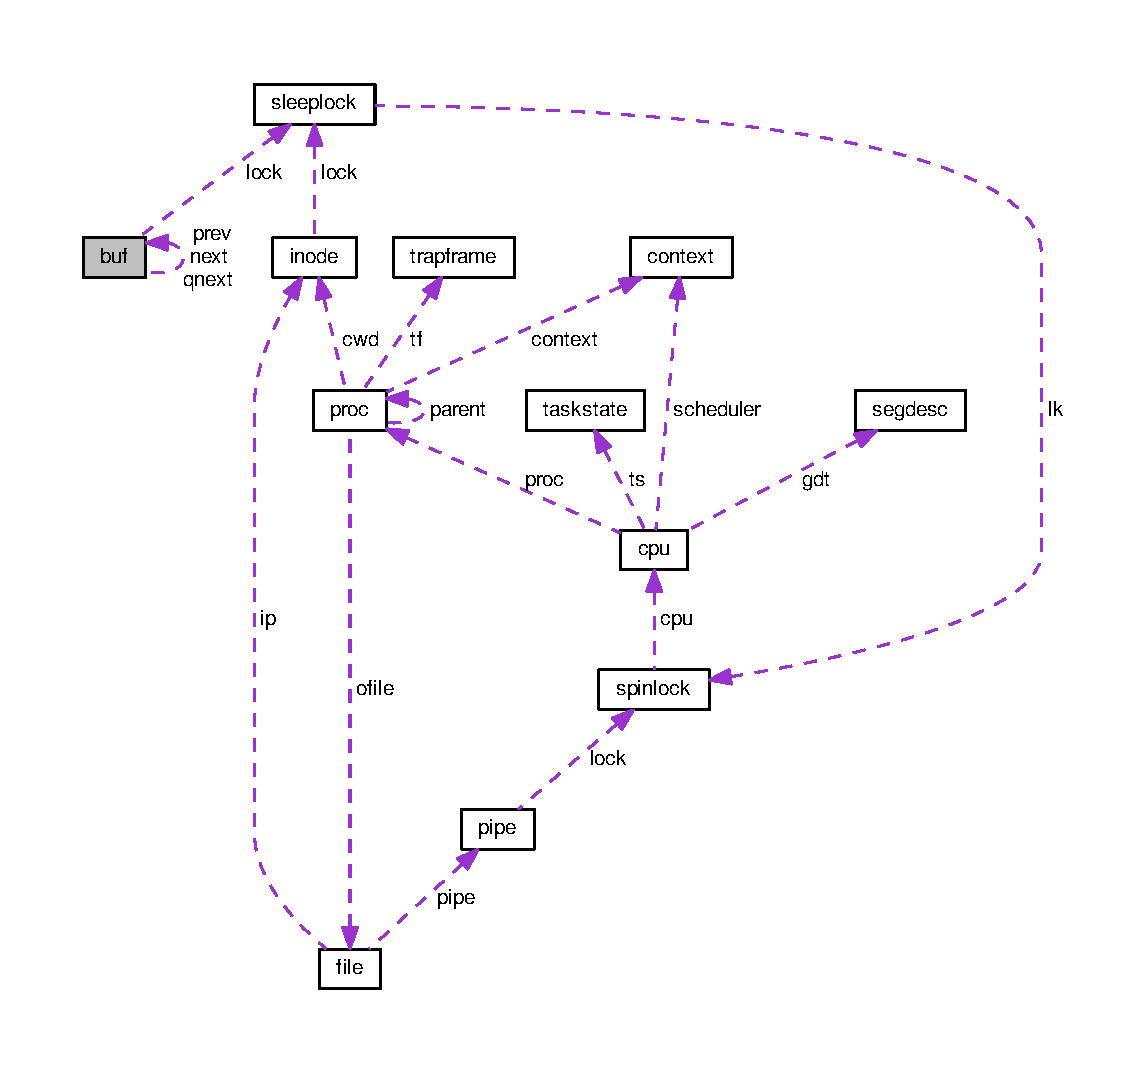
\includegraphics[width=350pt]{d6/d72/structbuf__coll__graph}
\end{center}
\end{figure}
\subsection*{Public Attributes}
\begin{DoxyCompactItemize}
\item 
int \hyperlink{structbuf_ae7d6b6c34fdeadb38970efd0554aa1a9}{flags}
\item 
\hyperlink{types_8h_a91ad9478d81a7aaf2593e8d9c3d06a14}{uint} \hyperlink{structbuf_ac96082c2b5f22133ac7092ef81487227}{dev}
\item 
\hyperlink{types_8h_a91ad9478d81a7aaf2593e8d9c3d06a14}{uint} \hyperlink{structbuf_a756b2bcc88008bef7f21d688aa4a7a48}{blockno}
\item 
struct \hyperlink{structsleeplock}{sleeplock} \hyperlink{structbuf_a626ad748d91d4bd7f4e65b74c73f2644}{lock}
\item 
\hyperlink{types_8h_a91ad9478d81a7aaf2593e8d9c3d06a14}{uint} \hyperlink{structbuf_aaf5efe777371aaeb9944508fd52adda5}{refcnt}
\item 
struct \hyperlink{structbuf}{buf} $\ast$ \hyperlink{structbuf_a930cab1e1b3751795d31bfd0291dff4a}{prev}
\item 
struct \hyperlink{structbuf}{buf} $\ast$ \hyperlink{structbuf_ab18c18abb22f07617619e9a74c71f51a}{next}
\item 
struct \hyperlink{structbuf}{buf} $\ast$ \hyperlink{structbuf_aba5c088c4da07a5ec88edfacdae9b85a}{qnext}
\item 
\hyperlink{types_8h_a65f85814a8290f9797005d3b28e7e5fc}{uchar} \hyperlink{structbuf_ab0ec38784ab94ed35e575cf6d33912d2}{data} \mbox{[}\hyperlink{fs_8h_a403cf3149c084cea115b85c90721039a}{B\+S\+I\+ZE}\mbox{]}
\end{DoxyCompactItemize}


\subsection{Member Data Documentation}
\index{buf@{buf}!blockno@{blockno}}
\index{blockno@{blockno}!buf@{buf}}
\subsubsection[{\texorpdfstring{blockno}{blockno}}]{\setlength{\rightskip}{0pt plus 5cm}{\bf uint} buf\+::blockno}\hypertarget{structbuf_a756b2bcc88008bef7f21d688aa4a7a48}{}\label{structbuf_a756b2bcc88008bef7f21d688aa4a7a48}
\index{buf@{buf}!data@{data}}
\index{data@{data}!buf@{buf}}
\subsubsection[{\texorpdfstring{data}{data}}]{\setlength{\rightskip}{0pt plus 5cm}{\bf uchar} buf\+::data\mbox{[}{\bf B\+S\+I\+ZE}\mbox{]}}\hypertarget{structbuf_ab0ec38784ab94ed35e575cf6d33912d2}{}\label{structbuf_ab0ec38784ab94ed35e575cf6d33912d2}
\index{buf@{buf}!dev@{dev}}
\index{dev@{dev}!buf@{buf}}
\subsubsection[{\texorpdfstring{dev}{dev}}]{\setlength{\rightskip}{0pt plus 5cm}{\bf uint} buf\+::dev}\hypertarget{structbuf_ac96082c2b5f22133ac7092ef81487227}{}\label{structbuf_ac96082c2b5f22133ac7092ef81487227}
\index{buf@{buf}!flags@{flags}}
\index{flags@{flags}!buf@{buf}}
\subsubsection[{\texorpdfstring{flags}{flags}}]{\setlength{\rightskip}{0pt plus 5cm}int buf\+::flags}\hypertarget{structbuf_ae7d6b6c34fdeadb38970efd0554aa1a9}{}\label{structbuf_ae7d6b6c34fdeadb38970efd0554aa1a9}
\index{buf@{buf}!lock@{lock}}
\index{lock@{lock}!buf@{buf}}
\subsubsection[{\texorpdfstring{lock}{lock}}]{\setlength{\rightskip}{0pt plus 5cm}struct {\bf sleeplock} buf\+::lock}\hypertarget{structbuf_a626ad748d91d4bd7f4e65b74c73f2644}{}\label{structbuf_a626ad748d91d4bd7f4e65b74c73f2644}
\index{buf@{buf}!next@{next}}
\index{next@{next}!buf@{buf}}
\subsubsection[{\texorpdfstring{next}{next}}]{\setlength{\rightskip}{0pt plus 5cm}struct {\bf buf}$\ast$ buf\+::next}\hypertarget{structbuf_ab18c18abb22f07617619e9a74c71f51a}{}\label{structbuf_ab18c18abb22f07617619e9a74c71f51a}
\index{buf@{buf}!prev@{prev}}
\index{prev@{prev}!buf@{buf}}
\subsubsection[{\texorpdfstring{prev}{prev}}]{\setlength{\rightskip}{0pt plus 5cm}struct {\bf buf}$\ast$ buf\+::prev}\hypertarget{structbuf_a930cab1e1b3751795d31bfd0291dff4a}{}\label{structbuf_a930cab1e1b3751795d31bfd0291dff4a}
\index{buf@{buf}!qnext@{qnext}}
\index{qnext@{qnext}!buf@{buf}}
\subsubsection[{\texorpdfstring{qnext}{qnext}}]{\setlength{\rightskip}{0pt plus 5cm}struct {\bf buf}$\ast$ buf\+::qnext}\hypertarget{structbuf_aba5c088c4da07a5ec88edfacdae9b85a}{}\label{structbuf_aba5c088c4da07a5ec88edfacdae9b85a}
\index{buf@{buf}!refcnt@{refcnt}}
\index{refcnt@{refcnt}!buf@{buf}}
\subsubsection[{\texorpdfstring{refcnt}{refcnt}}]{\setlength{\rightskip}{0pt plus 5cm}{\bf uint} buf\+::refcnt}\hypertarget{structbuf_aaf5efe777371aaeb9944508fd52adda5}{}\label{structbuf_aaf5efe777371aaeb9944508fd52adda5}


The documentation for this struct was generated from the following file\+:\begin{DoxyCompactItemize}
\item 
\hyperlink{buf_8h}{buf.\+h}\end{DoxyCompactItemize}

\hypertarget{structcontext}{}\section{context Struct Reference}
\label{structcontext}\index{context@{context}}


{\ttfamily \#include $<$proc.\+h$>$}

\subsection*{Public Attributes}
\begin{DoxyCompactItemize}
\item 
\hyperlink{types_8h_a91ad9478d81a7aaf2593e8d9c3d06a14}{uint} \hyperlink{structcontext_a9c926d583d00a615327b9b4a8fe0ab63}{edi}
\item 
\hyperlink{types_8h_a91ad9478d81a7aaf2593e8d9c3d06a14}{uint} \hyperlink{structcontext_a9596ea769c8681490bbc67fd1b0abc92}{esi}
\item 
\hyperlink{types_8h_a91ad9478d81a7aaf2593e8d9c3d06a14}{uint} \hyperlink{structcontext_ab1dd54ca1266e38df5943750224cd8d5}{ebx}
\item 
\hyperlink{types_8h_a91ad9478d81a7aaf2593e8d9c3d06a14}{uint} \hyperlink{structcontext_ac9640ddc2e90e4213ba9847bbe1b0e57}{ebp}
\item 
\hyperlink{types_8h_a91ad9478d81a7aaf2593e8d9c3d06a14}{uint} \hyperlink{structcontext_a0cfb49e5b03fd7bf12fa79d1a42be935}{eip}
\end{DoxyCompactItemize}


\subsection{Member Data Documentation}
\index{context@{context}!ebp@{ebp}}
\index{ebp@{ebp}!context@{context}}
\subsubsection[{\texorpdfstring{ebp}{ebp}}]{\setlength{\rightskip}{0pt plus 5cm}{\bf uint} context\+::ebp}\hypertarget{structcontext_ac9640ddc2e90e4213ba9847bbe1b0e57}{}\label{structcontext_ac9640ddc2e90e4213ba9847bbe1b0e57}
\index{context@{context}!ebx@{ebx}}
\index{ebx@{ebx}!context@{context}}
\subsubsection[{\texorpdfstring{ebx}{ebx}}]{\setlength{\rightskip}{0pt plus 5cm}{\bf uint} context\+::ebx}\hypertarget{structcontext_ab1dd54ca1266e38df5943750224cd8d5}{}\label{structcontext_ab1dd54ca1266e38df5943750224cd8d5}
\index{context@{context}!edi@{edi}}
\index{edi@{edi}!context@{context}}
\subsubsection[{\texorpdfstring{edi}{edi}}]{\setlength{\rightskip}{0pt plus 5cm}{\bf uint} context\+::edi}\hypertarget{structcontext_a9c926d583d00a615327b9b4a8fe0ab63}{}\label{structcontext_a9c926d583d00a615327b9b4a8fe0ab63}
\index{context@{context}!eip@{eip}}
\index{eip@{eip}!context@{context}}
\subsubsection[{\texorpdfstring{eip}{eip}}]{\setlength{\rightskip}{0pt plus 5cm}{\bf uint} context\+::eip}\hypertarget{structcontext_a0cfb49e5b03fd7bf12fa79d1a42be935}{}\label{structcontext_a0cfb49e5b03fd7bf12fa79d1a42be935}
\index{context@{context}!esi@{esi}}
\index{esi@{esi}!context@{context}}
\subsubsection[{\texorpdfstring{esi}{esi}}]{\setlength{\rightskip}{0pt plus 5cm}{\bf uint} context\+::esi}\hypertarget{structcontext_a9596ea769c8681490bbc67fd1b0abc92}{}\label{structcontext_a9596ea769c8681490bbc67fd1b0abc92}


The documentation for this struct was generated from the following file\+:\begin{DoxyCompactItemize}
\item 
\hyperlink{proc_8h}{proc.\+h}\end{DoxyCompactItemize}

\hypertarget{structcpu}{}\section{cpu Struct Reference}
\label{structcpu}\index{cpu@{cpu}}


{\ttfamily \#include $<$proc.\+h$>$}



Collaboration diagram for cpu\+:\nopagebreak
\begin{figure}[H]
\begin{center}
\leavevmode
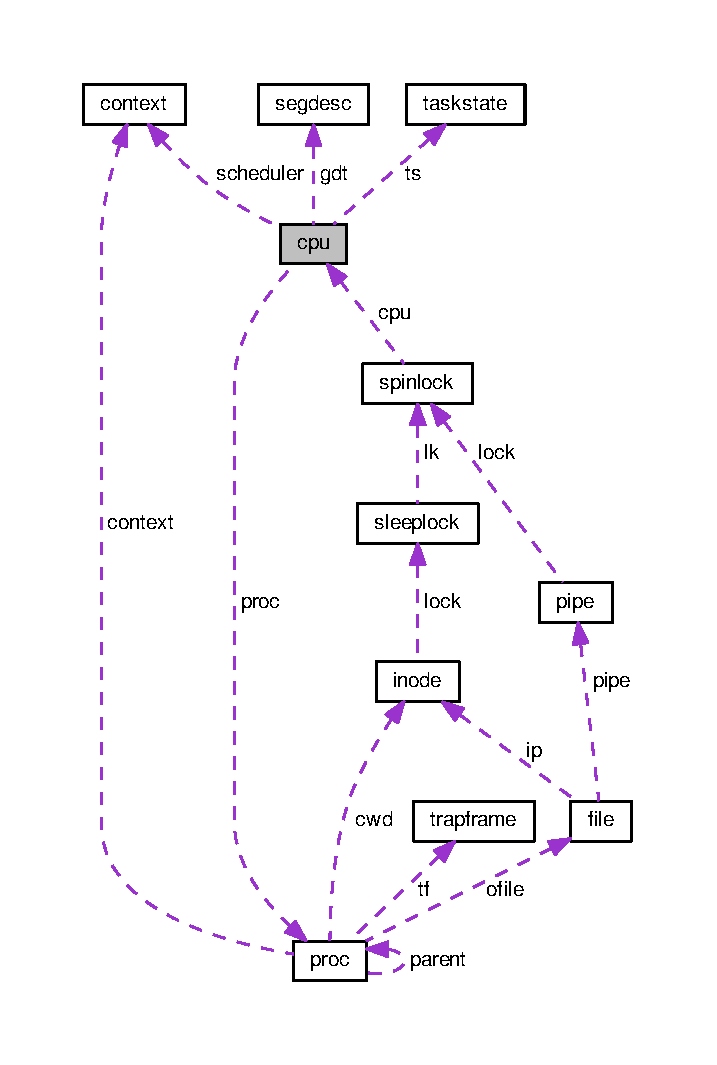
\includegraphics[width=344pt]{d0/de5/structcpu__coll__graph}
\end{center}
\end{figure}
\subsection*{Public Attributes}
\begin{DoxyCompactItemize}
\item 
\hyperlink{types_8h_a65f85814a8290f9797005d3b28e7e5fc}{uchar} \hyperlink{structcpu_ad08a3478ec15fc8bec1d9b6b5a0431db}{apicid}
\item 
struct \hyperlink{structcontext}{context} $\ast$ \hyperlink{structcpu_aaa1510fdf8a2230c033d04e13e4fdd9e}{scheduler}
\item 
struct \hyperlink{structtaskstate}{taskstate} \hyperlink{structcpu_a32e7b5aa877171c943d47038e818a159}{ts}
\item 
struct \hyperlink{structsegdesc}{segdesc} \hyperlink{structcpu_aee38fb8832f8e728538b2cee877d1c09}{gdt} \mbox{[}\hyperlink{mmu_8h_a2fca412c6ed6584438e96f43ccce030a}{N\+S\+E\+GS}\mbox{]}
\item 
volatile \hyperlink{types_8h_a91ad9478d81a7aaf2593e8d9c3d06a14}{uint} \hyperlink{structcpu_a869f6e0e1dbf69de0bdb3546f981847f}{started}
\item 
int \hyperlink{structcpu_a9ccad8ae031c295f86e96de26df24805}{ncli}
\item 
int \hyperlink{structcpu_a26fc271fea8af30d67fc2ae22ef0a82f}{intena}
\item 
struct \hyperlink{structproc}{proc} $\ast$ \hyperlink{structcpu_a9e71a6265904fd644875a9ea5a413c89}{proc}
\end{DoxyCompactItemize}


\subsection{Member Data Documentation}
\index{cpu@{cpu}!apicid@{apicid}}
\index{apicid@{apicid}!cpu@{cpu}}
\subsubsection[{\texorpdfstring{apicid}{apicid}}]{\setlength{\rightskip}{0pt plus 5cm}{\bf uchar} cpu\+::apicid}\hypertarget{structcpu_ad08a3478ec15fc8bec1d9b6b5a0431db}{}\label{structcpu_ad08a3478ec15fc8bec1d9b6b5a0431db}
\index{cpu@{cpu}!gdt@{gdt}}
\index{gdt@{gdt}!cpu@{cpu}}
\subsubsection[{\texorpdfstring{gdt}{gdt}}]{\setlength{\rightskip}{0pt plus 5cm}struct {\bf segdesc} cpu\+::gdt\mbox{[}{\bf N\+S\+E\+GS}\mbox{]}}\hypertarget{structcpu_aee38fb8832f8e728538b2cee877d1c09}{}\label{structcpu_aee38fb8832f8e728538b2cee877d1c09}
\index{cpu@{cpu}!intena@{intena}}
\index{intena@{intena}!cpu@{cpu}}
\subsubsection[{\texorpdfstring{intena}{intena}}]{\setlength{\rightskip}{0pt plus 5cm}int cpu\+::intena}\hypertarget{structcpu_a26fc271fea8af30d67fc2ae22ef0a82f}{}\label{structcpu_a26fc271fea8af30d67fc2ae22ef0a82f}
\index{cpu@{cpu}!ncli@{ncli}}
\index{ncli@{ncli}!cpu@{cpu}}
\subsubsection[{\texorpdfstring{ncli}{ncli}}]{\setlength{\rightskip}{0pt plus 5cm}int cpu\+::ncli}\hypertarget{structcpu_a9ccad8ae031c295f86e96de26df24805}{}\label{structcpu_a9ccad8ae031c295f86e96de26df24805}
\index{cpu@{cpu}!proc@{proc}}
\index{proc@{proc}!cpu@{cpu}}
\subsubsection[{\texorpdfstring{proc}{proc}}]{\setlength{\rightskip}{0pt plus 5cm}struct {\bf proc}$\ast$ cpu\+::proc}\hypertarget{structcpu_a9e71a6265904fd644875a9ea5a413c89}{}\label{structcpu_a9e71a6265904fd644875a9ea5a413c89}
\index{cpu@{cpu}!scheduler@{scheduler}}
\index{scheduler@{scheduler}!cpu@{cpu}}
\subsubsection[{\texorpdfstring{scheduler}{scheduler}}]{\setlength{\rightskip}{0pt plus 5cm}struct {\bf context}$\ast$ cpu\+::scheduler}\hypertarget{structcpu_aaa1510fdf8a2230c033d04e13e4fdd9e}{}\label{structcpu_aaa1510fdf8a2230c033d04e13e4fdd9e}
\index{cpu@{cpu}!started@{started}}
\index{started@{started}!cpu@{cpu}}
\subsubsection[{\texorpdfstring{started}{started}}]{\setlength{\rightskip}{0pt plus 5cm}volatile {\bf uint} cpu\+::started}\hypertarget{structcpu_a869f6e0e1dbf69de0bdb3546f981847f}{}\label{structcpu_a869f6e0e1dbf69de0bdb3546f981847f}
\index{cpu@{cpu}!ts@{ts}}
\index{ts@{ts}!cpu@{cpu}}
\subsubsection[{\texorpdfstring{ts}{ts}}]{\setlength{\rightskip}{0pt plus 5cm}struct {\bf taskstate} cpu\+::ts}\hypertarget{structcpu_a32e7b5aa877171c943d47038e818a159}{}\label{structcpu_a32e7b5aa877171c943d47038e818a159}


The documentation for this struct was generated from the following file\+:\begin{DoxyCompactItemize}
\item 
\hyperlink{proc_8h}{proc.\+h}\end{DoxyCompactItemize}

\hypertarget{structdevsw}{}\section{devsw Struct Reference}
\label{structdevsw}\index{devsw@{devsw}}


{\ttfamily \#include $<$file.\+h$>$}

\subsection*{Public Attributes}
\begin{DoxyCompactItemize}
\item 
int($\ast$ \hyperlink{structdevsw_a4efbe00d0031a1c9005ef2186947ea37}{read} )(struct \hyperlink{structinode}{inode} $\ast$, char $\ast$, int)
\item 
int($\ast$ \hyperlink{structdevsw_a87fd7af6c9a6fb8663fc206be7a233d4}{write} )(struct \hyperlink{structinode}{inode} $\ast$, char $\ast$, int)
\end{DoxyCompactItemize}


\subsection{Member Data Documentation}
\index{devsw@{devsw}!read@{read}}
\index{read@{read}!devsw@{devsw}}
\subsubsection[{\texorpdfstring{read}{read}}]{\setlength{\rightskip}{0pt plus 5cm}int($\ast$ devsw\+::read) (struct {\bf inode} $\ast$, char $\ast$, int)}\hypertarget{structdevsw_a4efbe00d0031a1c9005ef2186947ea37}{}\label{structdevsw_a4efbe00d0031a1c9005ef2186947ea37}
\index{devsw@{devsw}!write@{write}}
\index{write@{write}!devsw@{devsw}}
\subsubsection[{\texorpdfstring{write}{write}}]{\setlength{\rightskip}{0pt plus 5cm}int($\ast$ devsw\+::write) (struct {\bf inode} $\ast$, char $\ast$, int)}\hypertarget{structdevsw_a87fd7af6c9a6fb8663fc206be7a233d4}{}\label{structdevsw_a87fd7af6c9a6fb8663fc206be7a233d4}


The documentation for this struct was generated from the following file\+:\begin{DoxyCompactItemize}
\item 
\hyperlink{file_8h}{file.\+h}\end{DoxyCompactItemize}

\hypertarget{structdinode}{}\section{dinode Struct Reference}
\label{structdinode}\index{dinode@{dinode}}


{\ttfamily \#include $<$fs.\+h$>$}

\subsection*{Public Attributes}
\begin{DoxyCompactItemize}
\item 
short \hyperlink{structdinode_abf6b2a8476a803284f1c927fb3b82259}{type}
\item 
short \hyperlink{structdinode_aca8272002020f48219df175c986db257}{major}
\item 
short \hyperlink{structdinode_ae97965f85e7353313f85035e8fc63495}{minor}
\item 
short \hyperlink{structdinode_a105562253b461c11413c9a229ef15358}{nlink}
\item 
\hyperlink{types_8h_a91ad9478d81a7aaf2593e8d9c3d06a14}{uint} \hyperlink{structdinode_a990ad8ddf5f8c051fbbe95cf550d2164}{size}
\item 
\hyperlink{types_8h_a91ad9478d81a7aaf2593e8d9c3d06a14}{uint} \hyperlink{structdinode_a705729b3a39c10c0ba6927fc5e4e0563}{addrs} \mbox{[}\hyperlink{fs_8h_acd38e9532d4b3623f844b93c012a8e06}{N\+D\+I\+R\+E\+CT}+1\mbox{]}
\end{DoxyCompactItemize}


\subsection{Member Data Documentation}
\index{dinode@{dinode}!addrs@{addrs}}
\index{addrs@{addrs}!dinode@{dinode}}
\subsubsection[{\texorpdfstring{addrs}{addrs}}]{\setlength{\rightskip}{0pt plus 5cm}{\bf uint} dinode\+::addrs\mbox{[}{\bf N\+D\+I\+R\+E\+CT}+1\mbox{]}}\hypertarget{structdinode_a705729b3a39c10c0ba6927fc5e4e0563}{}\label{structdinode_a705729b3a39c10c0ba6927fc5e4e0563}
\index{dinode@{dinode}!major@{major}}
\index{major@{major}!dinode@{dinode}}
\subsubsection[{\texorpdfstring{major}{major}}]{\setlength{\rightskip}{0pt plus 5cm}short dinode\+::major}\hypertarget{structdinode_aca8272002020f48219df175c986db257}{}\label{structdinode_aca8272002020f48219df175c986db257}
\index{dinode@{dinode}!minor@{minor}}
\index{minor@{minor}!dinode@{dinode}}
\subsubsection[{\texorpdfstring{minor}{minor}}]{\setlength{\rightskip}{0pt plus 5cm}short dinode\+::minor}\hypertarget{structdinode_ae97965f85e7353313f85035e8fc63495}{}\label{structdinode_ae97965f85e7353313f85035e8fc63495}
\index{dinode@{dinode}!nlink@{nlink}}
\index{nlink@{nlink}!dinode@{dinode}}
\subsubsection[{\texorpdfstring{nlink}{nlink}}]{\setlength{\rightskip}{0pt plus 5cm}short dinode\+::nlink}\hypertarget{structdinode_a105562253b461c11413c9a229ef15358}{}\label{structdinode_a105562253b461c11413c9a229ef15358}
\index{dinode@{dinode}!size@{size}}
\index{size@{size}!dinode@{dinode}}
\subsubsection[{\texorpdfstring{size}{size}}]{\setlength{\rightskip}{0pt plus 5cm}{\bf uint} dinode\+::size}\hypertarget{structdinode_a990ad8ddf5f8c051fbbe95cf550d2164}{}\label{structdinode_a990ad8ddf5f8c051fbbe95cf550d2164}
\index{dinode@{dinode}!type@{type}}
\index{type@{type}!dinode@{dinode}}
\subsubsection[{\texorpdfstring{type}{type}}]{\setlength{\rightskip}{0pt plus 5cm}short dinode\+::type}\hypertarget{structdinode_abf6b2a8476a803284f1c927fb3b82259}{}\label{structdinode_abf6b2a8476a803284f1c927fb3b82259}


The documentation for this struct was generated from the following file\+:\begin{DoxyCompactItemize}
\item 
\hyperlink{fs_8h}{fs.\+h}\end{DoxyCompactItemize}

\hypertarget{structdirent}{}\section{dirent Struct Reference}
\label{structdirent}\index{dirent@{dirent}}


{\ttfamily \#include $<$fs.\+h$>$}

\subsection*{Public Attributes}
\begin{DoxyCompactItemize}
\item 
\hyperlink{types_8h_ab95f123a6c9bcfee6a343170ef8c5f69}{ushort} \hyperlink{structdirent_a68698c303a46d2a34232a2226629ac79}{inum}
\item 
char \hyperlink{structdirent_a4e08a84dbac9b9f6a3e006151855d14d}{name} \mbox{[}\hyperlink{fs_8h_a48246fb9e5cb7f6a71ebc9ebc2f06562}{D\+I\+R\+S\+IZ}\mbox{]}
\end{DoxyCompactItemize}


\subsection{Member Data Documentation}
\index{dirent@{dirent}!inum@{inum}}
\index{inum@{inum}!dirent@{dirent}}
\subsubsection[{\texorpdfstring{inum}{inum}}]{\setlength{\rightskip}{0pt plus 5cm}{\bf ushort} dirent\+::inum}\hypertarget{structdirent_a68698c303a46d2a34232a2226629ac79}{}\label{structdirent_a68698c303a46d2a34232a2226629ac79}
\index{dirent@{dirent}!name@{name}}
\index{name@{name}!dirent@{dirent}}
\subsubsection[{\texorpdfstring{name}{name}}]{\setlength{\rightskip}{0pt plus 5cm}char dirent\+::name\mbox{[}{\bf D\+I\+R\+S\+IZ}\mbox{]}}\hypertarget{structdirent_a4e08a84dbac9b9f6a3e006151855d14d}{}\label{structdirent_a4e08a84dbac9b9f6a3e006151855d14d}


The documentation for this struct was generated from the following file\+:\begin{DoxyCompactItemize}
\item 
\hyperlink{fs_8h}{fs.\+h}\end{DoxyCompactItemize}

\hypertarget{structelfhdr}{}\section{elfhdr Struct Reference}
\label{structelfhdr}\index{elfhdr@{elfhdr}}


{\ttfamily \#include $<$elf.\+h$>$}

\subsection*{Public Attributes}
\begin{DoxyCompactItemize}
\item 
\hyperlink{types_8h_a91ad9478d81a7aaf2593e8d9c3d06a14}{uint} \hyperlink{structelfhdr_a28ee8116d69b533277311c5f3773b6b2}{magic}
\item 
\hyperlink{types_8h_a65f85814a8290f9797005d3b28e7e5fc}{uchar} \hyperlink{structelfhdr_a22ec6f2383f0488ee18a18673398f201}{elf} \mbox{[}12\mbox{]}
\item 
\hyperlink{types_8h_ab95f123a6c9bcfee6a343170ef8c5f69}{ushort} \hyperlink{structelfhdr_a2cd2eaf0c952e30f8196890787ef68fe}{type}
\item 
\hyperlink{types_8h_ab95f123a6c9bcfee6a343170ef8c5f69}{ushort} \hyperlink{structelfhdr_a17113c58d39b044bb1ae78733a8c68fc}{machine}
\item 
\hyperlink{types_8h_a91ad9478d81a7aaf2593e8d9c3d06a14}{uint} \hyperlink{structelfhdr_abb1c8274f47cfdbbcefe44af2d5c723d}{version}
\item 
\hyperlink{types_8h_a91ad9478d81a7aaf2593e8d9c3d06a14}{uint} \hyperlink{structelfhdr_ad40755e1b2c6efc3ec0ad95889f743a5}{entry}
\item 
\hyperlink{types_8h_a91ad9478d81a7aaf2593e8d9c3d06a14}{uint} \hyperlink{structelfhdr_a1d463f67fcf951c06cfaa37850004c51}{phoff}
\item 
\hyperlink{types_8h_a91ad9478d81a7aaf2593e8d9c3d06a14}{uint} \hyperlink{structelfhdr_a465ccdf83d0e26d129d723a493a6e764}{shoff}
\item 
\hyperlink{types_8h_a91ad9478d81a7aaf2593e8d9c3d06a14}{uint} \hyperlink{structelfhdr_a2f1e0957c83938630ef0ed074830df03}{flags}
\item 
\hyperlink{types_8h_ab95f123a6c9bcfee6a343170ef8c5f69}{ushort} \hyperlink{structelfhdr_aeffe5743cc720e5795af5d17b6fd6928}{ehsize}
\item 
\hyperlink{types_8h_ab95f123a6c9bcfee6a343170ef8c5f69}{ushort} \hyperlink{structelfhdr_ac636a4a9c4c61933c6044275ed687bc9}{phentsize}
\item 
\hyperlink{types_8h_ab95f123a6c9bcfee6a343170ef8c5f69}{ushort} \hyperlink{structelfhdr_a3eff58d58a3ee83aa53d7ffdebdb6b5b}{phnum}
\item 
\hyperlink{types_8h_ab95f123a6c9bcfee6a343170ef8c5f69}{ushort} \hyperlink{structelfhdr_aeedc5375e3f67e8dda6351e0e80b8e02}{shentsize}
\item 
\hyperlink{types_8h_ab95f123a6c9bcfee6a343170ef8c5f69}{ushort} \hyperlink{structelfhdr_aebf9526933b9f0502bdbafacce3734c1}{shnum}
\item 
\hyperlink{types_8h_ab95f123a6c9bcfee6a343170ef8c5f69}{ushort} \hyperlink{structelfhdr_a84f3d7712c99bfea3f4be42728dc0a0e}{shstrndx}
\end{DoxyCompactItemize}


\subsection{Member Data Documentation}
\index{elfhdr@{elfhdr}!ehsize@{ehsize}}
\index{ehsize@{ehsize}!elfhdr@{elfhdr}}
\subsubsection[{\texorpdfstring{ehsize}{ehsize}}]{\setlength{\rightskip}{0pt plus 5cm}{\bf ushort} elfhdr\+::ehsize}\hypertarget{structelfhdr_aeffe5743cc720e5795af5d17b6fd6928}{}\label{structelfhdr_aeffe5743cc720e5795af5d17b6fd6928}
\index{elfhdr@{elfhdr}!elf@{elf}}
\index{elf@{elf}!elfhdr@{elfhdr}}
\subsubsection[{\texorpdfstring{elf}{elf}}]{\setlength{\rightskip}{0pt plus 5cm}{\bf uchar} elfhdr\+::elf\mbox{[}12\mbox{]}}\hypertarget{structelfhdr_a22ec6f2383f0488ee18a18673398f201}{}\label{structelfhdr_a22ec6f2383f0488ee18a18673398f201}
\index{elfhdr@{elfhdr}!entry@{entry}}
\index{entry@{entry}!elfhdr@{elfhdr}}
\subsubsection[{\texorpdfstring{entry}{entry}}]{\setlength{\rightskip}{0pt plus 5cm}{\bf uint} elfhdr\+::entry}\hypertarget{structelfhdr_ad40755e1b2c6efc3ec0ad95889f743a5}{}\label{structelfhdr_ad40755e1b2c6efc3ec0ad95889f743a5}
\index{elfhdr@{elfhdr}!flags@{flags}}
\index{flags@{flags}!elfhdr@{elfhdr}}
\subsubsection[{\texorpdfstring{flags}{flags}}]{\setlength{\rightskip}{0pt plus 5cm}{\bf uint} elfhdr\+::flags}\hypertarget{structelfhdr_a2f1e0957c83938630ef0ed074830df03}{}\label{structelfhdr_a2f1e0957c83938630ef0ed074830df03}
\index{elfhdr@{elfhdr}!machine@{machine}}
\index{machine@{machine}!elfhdr@{elfhdr}}
\subsubsection[{\texorpdfstring{machine}{machine}}]{\setlength{\rightskip}{0pt plus 5cm}{\bf ushort} elfhdr\+::machine}\hypertarget{structelfhdr_a17113c58d39b044bb1ae78733a8c68fc}{}\label{structelfhdr_a17113c58d39b044bb1ae78733a8c68fc}
\index{elfhdr@{elfhdr}!magic@{magic}}
\index{magic@{magic}!elfhdr@{elfhdr}}
\subsubsection[{\texorpdfstring{magic}{magic}}]{\setlength{\rightskip}{0pt plus 5cm}{\bf uint} elfhdr\+::magic}\hypertarget{structelfhdr_a28ee8116d69b533277311c5f3773b6b2}{}\label{structelfhdr_a28ee8116d69b533277311c5f3773b6b2}
\index{elfhdr@{elfhdr}!phentsize@{phentsize}}
\index{phentsize@{phentsize}!elfhdr@{elfhdr}}
\subsubsection[{\texorpdfstring{phentsize}{phentsize}}]{\setlength{\rightskip}{0pt plus 5cm}{\bf ushort} elfhdr\+::phentsize}\hypertarget{structelfhdr_ac636a4a9c4c61933c6044275ed687bc9}{}\label{structelfhdr_ac636a4a9c4c61933c6044275ed687bc9}
\index{elfhdr@{elfhdr}!phnum@{phnum}}
\index{phnum@{phnum}!elfhdr@{elfhdr}}
\subsubsection[{\texorpdfstring{phnum}{phnum}}]{\setlength{\rightskip}{0pt plus 5cm}{\bf ushort} elfhdr\+::phnum}\hypertarget{structelfhdr_a3eff58d58a3ee83aa53d7ffdebdb6b5b}{}\label{structelfhdr_a3eff58d58a3ee83aa53d7ffdebdb6b5b}
\index{elfhdr@{elfhdr}!phoff@{phoff}}
\index{phoff@{phoff}!elfhdr@{elfhdr}}
\subsubsection[{\texorpdfstring{phoff}{phoff}}]{\setlength{\rightskip}{0pt plus 5cm}{\bf uint} elfhdr\+::phoff}\hypertarget{structelfhdr_a1d463f67fcf951c06cfaa37850004c51}{}\label{structelfhdr_a1d463f67fcf951c06cfaa37850004c51}
\index{elfhdr@{elfhdr}!shentsize@{shentsize}}
\index{shentsize@{shentsize}!elfhdr@{elfhdr}}
\subsubsection[{\texorpdfstring{shentsize}{shentsize}}]{\setlength{\rightskip}{0pt plus 5cm}{\bf ushort} elfhdr\+::shentsize}\hypertarget{structelfhdr_aeedc5375e3f67e8dda6351e0e80b8e02}{}\label{structelfhdr_aeedc5375e3f67e8dda6351e0e80b8e02}
\index{elfhdr@{elfhdr}!shnum@{shnum}}
\index{shnum@{shnum}!elfhdr@{elfhdr}}
\subsubsection[{\texorpdfstring{shnum}{shnum}}]{\setlength{\rightskip}{0pt plus 5cm}{\bf ushort} elfhdr\+::shnum}\hypertarget{structelfhdr_aebf9526933b9f0502bdbafacce3734c1}{}\label{structelfhdr_aebf9526933b9f0502bdbafacce3734c1}
\index{elfhdr@{elfhdr}!shoff@{shoff}}
\index{shoff@{shoff}!elfhdr@{elfhdr}}
\subsubsection[{\texorpdfstring{shoff}{shoff}}]{\setlength{\rightskip}{0pt plus 5cm}{\bf uint} elfhdr\+::shoff}\hypertarget{structelfhdr_a465ccdf83d0e26d129d723a493a6e764}{}\label{structelfhdr_a465ccdf83d0e26d129d723a493a6e764}
\index{elfhdr@{elfhdr}!shstrndx@{shstrndx}}
\index{shstrndx@{shstrndx}!elfhdr@{elfhdr}}
\subsubsection[{\texorpdfstring{shstrndx}{shstrndx}}]{\setlength{\rightskip}{0pt plus 5cm}{\bf ushort} elfhdr\+::shstrndx}\hypertarget{structelfhdr_a84f3d7712c99bfea3f4be42728dc0a0e}{}\label{structelfhdr_a84f3d7712c99bfea3f4be42728dc0a0e}
\index{elfhdr@{elfhdr}!type@{type}}
\index{type@{type}!elfhdr@{elfhdr}}
\subsubsection[{\texorpdfstring{type}{type}}]{\setlength{\rightskip}{0pt plus 5cm}{\bf ushort} elfhdr\+::type}\hypertarget{structelfhdr_a2cd2eaf0c952e30f8196890787ef68fe}{}\label{structelfhdr_a2cd2eaf0c952e30f8196890787ef68fe}
\index{elfhdr@{elfhdr}!version@{version}}
\index{version@{version}!elfhdr@{elfhdr}}
\subsubsection[{\texorpdfstring{version}{version}}]{\setlength{\rightskip}{0pt plus 5cm}{\bf uint} elfhdr\+::version}\hypertarget{structelfhdr_abb1c8274f47cfdbbcefe44af2d5c723d}{}\label{structelfhdr_abb1c8274f47cfdbbcefe44af2d5c723d}


The documentation for this struct was generated from the following file\+:\begin{DoxyCompactItemize}
\item 
\hyperlink{elf_8h}{elf.\+h}\end{DoxyCompactItemize}

\hypertarget{structfile}{}\section{file Struct Reference}
\label{structfile}\index{file@{file}}


{\ttfamily \#include $<$file.\+h$>$}



Collaboration diagram for file\+:\nopagebreak
\begin{figure}[H]
\begin{center}
\leavevmode
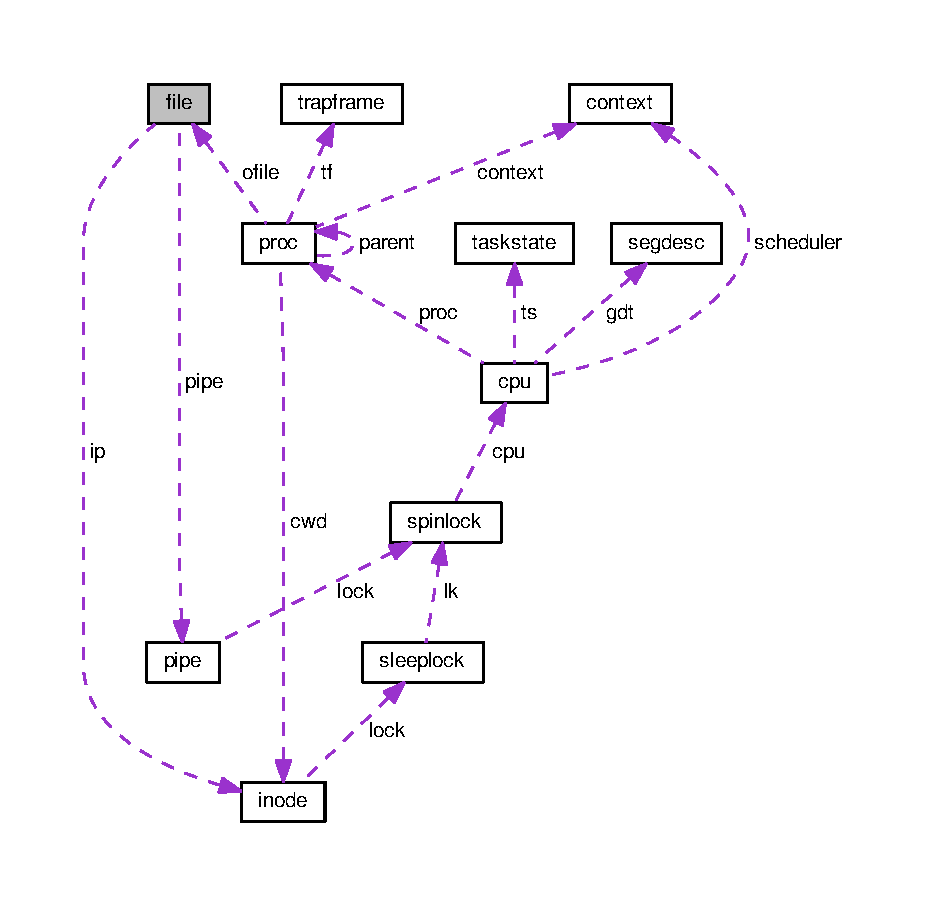
\includegraphics[width=350pt]{d9/da3/structfile__coll__graph}
\end{center}
\end{figure}
\subsection*{Public Types}
\begin{DoxyCompactItemize}
\item 
enum \{ \hyperlink{structfile_a4aeeba6a286e58966d853aa1f510d3d5a224e095442d50a6bd1058fd742fb68c7}{F\+D\+\_\+\+N\+O\+NE}, 
\hyperlink{structfile_a4aeeba6a286e58966d853aa1f510d3d5a59fcf59caf6e70c3cc3cc48291b89752}{F\+D\+\_\+\+P\+I\+PE}, 
\hyperlink{structfile_a4aeeba6a286e58966d853aa1f510d3d5aa5d8c5e0d95ed88367e96ecebfdf326d}{F\+D\+\_\+\+I\+N\+O\+DE}
 \}
\end{DoxyCompactItemize}
\subsection*{Public Attributes}
\begin{DoxyCompactItemize}
\item 
enum file\+:: \{ ... \}  \hyperlink{structfile_a7dee40626182d2568f513525b2e657bb}{type}
\item 
int \hyperlink{structfile_a41c818f828adea488058bca63e4df23f}{ref}
\item 
char \hyperlink{structfile_a0c5c8eced8bc562dbbecc8d450a6b646}{readable}
\item 
char \hyperlink{structfile_a6e1b641ea1551ac4316a0c11a683df45}{writable}
\item 
struct \hyperlink{structpipe}{pipe} $\ast$ \hyperlink{structfile_a19d83a8d6cb47902fe8c762d2798c198}{pipe}
\item 
struct \hyperlink{structinode}{inode} $\ast$ \hyperlink{structfile_a4fd095f927715574dc2a4f243690e508}{ip}
\item 
\hyperlink{types_8h_a91ad9478d81a7aaf2593e8d9c3d06a14}{uint} \hyperlink{structfile_a94a911be6cc1b1326728392d8b40150d}{off}
\end{DoxyCompactItemize}


\subsection{Member Enumeration Documentation}
\subsubsection[{\texorpdfstring{anonymous enum}{anonymous enum}}]{\setlength{\rightskip}{0pt plus 5cm}anonymous enum}\hypertarget{structfile_a4aeeba6a286e58966d853aa1f510d3d5}{}\label{structfile_a4aeeba6a286e58966d853aa1f510d3d5}
\begin{Desc}
\item[Enumerator]\par
\begin{description}
\index{F\+D\+\_\+\+N\+O\+NE@{F\+D\+\_\+\+N\+O\+NE}!file@{file}}\index{file@{file}!F\+D\+\_\+\+N\+O\+NE@{F\+D\+\_\+\+N\+O\+NE}}\item[{\em 
F\+D\+\_\+\+N\+O\+NE\hypertarget{structfile_a4aeeba6a286e58966d853aa1f510d3d5a224e095442d50a6bd1058fd742fb68c7}{}\label{structfile_a4aeeba6a286e58966d853aa1f510d3d5a224e095442d50a6bd1058fd742fb68c7}
}]\index{F\+D\+\_\+\+P\+I\+PE@{F\+D\+\_\+\+P\+I\+PE}!file@{file}}\index{file@{file}!F\+D\+\_\+\+P\+I\+PE@{F\+D\+\_\+\+P\+I\+PE}}\item[{\em 
F\+D\+\_\+\+P\+I\+PE\hypertarget{structfile_a4aeeba6a286e58966d853aa1f510d3d5a59fcf59caf6e70c3cc3cc48291b89752}{}\label{structfile_a4aeeba6a286e58966d853aa1f510d3d5a59fcf59caf6e70c3cc3cc48291b89752}
}]\index{F\+D\+\_\+\+I\+N\+O\+DE@{F\+D\+\_\+\+I\+N\+O\+DE}!file@{file}}\index{file@{file}!F\+D\+\_\+\+I\+N\+O\+DE@{F\+D\+\_\+\+I\+N\+O\+DE}}\item[{\em 
F\+D\+\_\+\+I\+N\+O\+DE\hypertarget{structfile_a4aeeba6a286e58966d853aa1f510d3d5aa5d8c5e0d95ed88367e96ecebfdf326d}{}\label{structfile_a4aeeba6a286e58966d853aa1f510d3d5aa5d8c5e0d95ed88367e96ecebfdf326d}
}]\end{description}
\end{Desc}


\subsection{Member Data Documentation}
\index{file@{file}!ip@{ip}}
\index{ip@{ip}!file@{file}}
\subsubsection[{\texorpdfstring{ip}{ip}}]{\setlength{\rightskip}{0pt plus 5cm}struct {\bf inode}$\ast$ file\+::ip}\hypertarget{structfile_a4fd095f927715574dc2a4f243690e508}{}\label{structfile_a4fd095f927715574dc2a4f243690e508}
\index{file@{file}!off@{off}}
\index{off@{off}!file@{file}}
\subsubsection[{\texorpdfstring{off}{off}}]{\setlength{\rightskip}{0pt plus 5cm}{\bf uint} file\+::off}\hypertarget{structfile_a94a911be6cc1b1326728392d8b40150d}{}\label{structfile_a94a911be6cc1b1326728392d8b40150d}
\index{file@{file}!pipe@{pipe}}
\index{pipe@{pipe}!file@{file}}
\subsubsection[{\texorpdfstring{pipe}{pipe}}]{\setlength{\rightskip}{0pt plus 5cm}struct {\bf pipe}$\ast$ file\+::pipe}\hypertarget{structfile_a19d83a8d6cb47902fe8c762d2798c198}{}\label{structfile_a19d83a8d6cb47902fe8c762d2798c198}
\index{file@{file}!readable@{readable}}
\index{readable@{readable}!file@{file}}
\subsubsection[{\texorpdfstring{readable}{readable}}]{\setlength{\rightskip}{0pt plus 5cm}char file\+::readable}\hypertarget{structfile_a0c5c8eced8bc562dbbecc8d450a6b646}{}\label{structfile_a0c5c8eced8bc562dbbecc8d450a6b646}
\index{file@{file}!ref@{ref}}
\index{ref@{ref}!file@{file}}
\subsubsection[{\texorpdfstring{ref}{ref}}]{\setlength{\rightskip}{0pt plus 5cm}int file\+::ref}\hypertarget{structfile_a41c818f828adea488058bca63e4df23f}{}\label{structfile_a41c818f828adea488058bca63e4df23f}
\index{file@{file}!type@{type}}
\index{type@{type}!file@{file}}
\subsubsection[{\texorpdfstring{type}{type}}]{\setlength{\rightskip}{0pt plus 5cm}enum \{ ... \}   file\+::type}\hypertarget{structfile_a7dee40626182d2568f513525b2e657bb}{}\label{structfile_a7dee40626182d2568f513525b2e657bb}
\index{file@{file}!writable@{writable}}
\index{writable@{writable}!file@{file}}
\subsubsection[{\texorpdfstring{writable}{writable}}]{\setlength{\rightskip}{0pt plus 5cm}char file\+::writable}\hypertarget{structfile_a6e1b641ea1551ac4316a0c11a683df45}{}\label{structfile_a6e1b641ea1551ac4316a0c11a683df45}


The documentation for this struct was generated from the following file\+:\begin{DoxyCompactItemize}
\item 
\hyperlink{file_8h}{file.\+h}\end{DoxyCompactItemize}

\hypertarget{structgatedesc}{}\section{gatedesc Struct Reference}
\label{structgatedesc}\index{gatedesc@{gatedesc}}


{\ttfamily \#include $<$mmu.\+h$>$}

\subsection*{Public Attributes}
\begin{DoxyCompactItemize}
\item 
\hyperlink{types_8h_a91ad9478d81a7aaf2593e8d9c3d06a14}{uint} \hyperlink{structgatedesc_a4f7268ba32b6a8b3963aa6d23e51af59}{off\+\_\+15\+\_\+0}\+: 16
\item 
\hyperlink{types_8h_a91ad9478d81a7aaf2593e8d9c3d06a14}{uint} \hyperlink{structgatedesc_a53e768c461dce9cc97048e7d19351af1}{cs}\+: 16
\item 
\hyperlink{types_8h_a91ad9478d81a7aaf2593e8d9c3d06a14}{uint} \hyperlink{structgatedesc_a9b41bea284fe0922c440f4c253e926ff}{args}\+: 5
\item 
\hyperlink{types_8h_a91ad9478d81a7aaf2593e8d9c3d06a14}{uint} \hyperlink{structgatedesc_ad11779f5ce40e53a8feb3dfdaf3f0ee5}{rsv1}\+: 3
\item 
\hyperlink{types_8h_a91ad9478d81a7aaf2593e8d9c3d06a14}{uint} \hyperlink{structgatedesc_a41d6e5fb9bb27699bdb7d729c67ff32c}{type}\+: 4
\item 
\hyperlink{types_8h_a91ad9478d81a7aaf2593e8d9c3d06a14}{uint} \hyperlink{structgatedesc_a54d731df342be3a775cc847a3dab1a53}{s}\+: 1
\item 
\hyperlink{types_8h_a91ad9478d81a7aaf2593e8d9c3d06a14}{uint} \hyperlink{structgatedesc_a4c62f5618440769c78ed976cae23c13d}{dpl}\+: 2
\item 
\hyperlink{types_8h_a91ad9478d81a7aaf2593e8d9c3d06a14}{uint} \hyperlink{structgatedesc_a5f754b650dc96be286cbc74e69da6a81}{p}\+: 1
\item 
\hyperlink{types_8h_a91ad9478d81a7aaf2593e8d9c3d06a14}{uint} \hyperlink{structgatedesc_af388a77c8f2a8a8c0bd1ca74a7dbaef7}{off\+\_\+31\+\_\+16}\+: 16
\end{DoxyCompactItemize}


\subsection{Member Data Documentation}
\index{gatedesc@{gatedesc}!args@{args}}
\index{args@{args}!gatedesc@{gatedesc}}
\subsubsection[{\texorpdfstring{args}{args}}]{\setlength{\rightskip}{0pt plus 5cm}{\bf uint} gatedesc\+::args}\hypertarget{structgatedesc_a9b41bea284fe0922c440f4c253e926ff}{}\label{structgatedesc_a9b41bea284fe0922c440f4c253e926ff}
\index{gatedesc@{gatedesc}!cs@{cs}}
\index{cs@{cs}!gatedesc@{gatedesc}}
\subsubsection[{\texorpdfstring{cs}{cs}}]{\setlength{\rightskip}{0pt plus 5cm}{\bf uint} gatedesc\+::cs}\hypertarget{structgatedesc_a53e768c461dce9cc97048e7d19351af1}{}\label{structgatedesc_a53e768c461dce9cc97048e7d19351af1}
\index{gatedesc@{gatedesc}!dpl@{dpl}}
\index{dpl@{dpl}!gatedesc@{gatedesc}}
\subsubsection[{\texorpdfstring{dpl}{dpl}}]{\setlength{\rightskip}{0pt plus 5cm}{\bf uint} gatedesc\+::dpl}\hypertarget{structgatedesc_a4c62f5618440769c78ed976cae23c13d}{}\label{structgatedesc_a4c62f5618440769c78ed976cae23c13d}
\index{gatedesc@{gatedesc}!off\+\_\+15\+\_\+0@{off\+\_\+15\+\_\+0}}
\index{off\+\_\+15\+\_\+0@{off\+\_\+15\+\_\+0}!gatedesc@{gatedesc}}
\subsubsection[{\texorpdfstring{off\+\_\+15\+\_\+0}{off_15_0}}]{\setlength{\rightskip}{0pt plus 5cm}{\bf uint} gatedesc\+::off\+\_\+15\+\_\+0}\hypertarget{structgatedesc_a4f7268ba32b6a8b3963aa6d23e51af59}{}\label{structgatedesc_a4f7268ba32b6a8b3963aa6d23e51af59}
\index{gatedesc@{gatedesc}!off\+\_\+31\+\_\+16@{off\+\_\+31\+\_\+16}}
\index{off\+\_\+31\+\_\+16@{off\+\_\+31\+\_\+16}!gatedesc@{gatedesc}}
\subsubsection[{\texorpdfstring{off\+\_\+31\+\_\+16}{off_31_16}}]{\setlength{\rightskip}{0pt plus 5cm}{\bf uint} gatedesc\+::off\+\_\+31\+\_\+16}\hypertarget{structgatedesc_af388a77c8f2a8a8c0bd1ca74a7dbaef7}{}\label{structgatedesc_af388a77c8f2a8a8c0bd1ca74a7dbaef7}
\index{gatedesc@{gatedesc}!p@{p}}
\index{p@{p}!gatedesc@{gatedesc}}
\subsubsection[{\texorpdfstring{p}{p}}]{\setlength{\rightskip}{0pt plus 5cm}{\bf uint} gatedesc\+::p}\hypertarget{structgatedesc_a5f754b650dc96be286cbc74e69da6a81}{}\label{structgatedesc_a5f754b650dc96be286cbc74e69da6a81}
\index{gatedesc@{gatedesc}!rsv1@{rsv1}}
\index{rsv1@{rsv1}!gatedesc@{gatedesc}}
\subsubsection[{\texorpdfstring{rsv1}{rsv1}}]{\setlength{\rightskip}{0pt plus 5cm}{\bf uint} gatedesc\+::rsv1}\hypertarget{structgatedesc_ad11779f5ce40e53a8feb3dfdaf3f0ee5}{}\label{structgatedesc_ad11779f5ce40e53a8feb3dfdaf3f0ee5}
\index{gatedesc@{gatedesc}!s@{s}}
\index{s@{s}!gatedesc@{gatedesc}}
\subsubsection[{\texorpdfstring{s}{s}}]{\setlength{\rightskip}{0pt plus 5cm}{\bf uint} gatedesc\+::s}\hypertarget{structgatedesc_a54d731df342be3a775cc847a3dab1a53}{}\label{structgatedesc_a54d731df342be3a775cc847a3dab1a53}
\index{gatedesc@{gatedesc}!type@{type}}
\index{type@{type}!gatedesc@{gatedesc}}
\subsubsection[{\texorpdfstring{type}{type}}]{\setlength{\rightskip}{0pt plus 5cm}{\bf uint} gatedesc\+::type}\hypertarget{structgatedesc_a41d6e5fb9bb27699bdb7d729c67ff32c}{}\label{structgatedesc_a41d6e5fb9bb27699bdb7d729c67ff32c}


The documentation for this struct was generated from the following file\+:\begin{DoxyCompactItemize}
\item 
\hyperlink{mmu_8h}{mmu.\+h}\end{DoxyCompactItemize}

\hypertarget{unionheader}{}\section{header Union Reference}
\label{unionheader}\index{header@{header}}


Collaboration diagram for header\+:\nopagebreak
\begin{figure}[H]
\begin{center}
\leavevmode
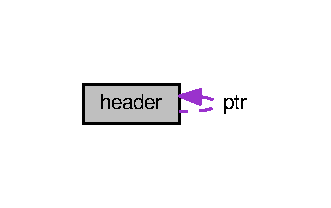
\includegraphics[width=159pt]{df/d0e/unionheader__coll__graph}
\end{center}
\end{figure}
\subsection*{Public Attributes}
\begin{DoxyCompactItemize}
\item 
\begin{tabbing}
xx\=xx\=xx\=xx\=xx\=xx\=xx\=xx\=xx\=\kill
struct \{\\
\>union \hyperlink{unionheader}{header} $\ast$ \hyperlink{unionheader_adcb7a02e18836885c802789f6a6c99fd}{ptr}\\
\>\hyperlink{types_8h_a91ad9478d81a7aaf2593e8d9c3d06a14}{uint} \hyperlink{unionheader_a70db454b20b4a40995532b7ea029a527}{size}\\
\} \hyperlink{unionheader_a3d684c1d6a9465b92eb26550d38ce659}{s}\\

\end{tabbing}\item 
\hyperlink{umalloc_8c_aa508dd61e627680e57643837d292d89f}{Align} \hyperlink{unionheader_a2f321dbb657408f93d0c585f55951bdb}{x}
\end{DoxyCompactItemize}


\subsection{Member Data Documentation}
\index{header@{header}!ptr@{ptr}}
\index{ptr@{ptr}!header@{header}}
\subsubsection[{\texorpdfstring{ptr}{ptr}}]{\setlength{\rightskip}{0pt plus 5cm}union {\bf header}$\ast$ header\+::ptr}\hypertarget{unionheader_adcb7a02e18836885c802789f6a6c99fd}{}\label{unionheader_adcb7a02e18836885c802789f6a6c99fd}
\index{header@{header}!s@{s}}
\index{s@{s}!header@{header}}
\subsubsection[{\texorpdfstring{s}{s}}]{\setlength{\rightskip}{0pt plus 5cm}struct \{ ... \}   header\+::s}\hypertarget{unionheader_a3d684c1d6a9465b92eb26550d38ce659}{}\label{unionheader_a3d684c1d6a9465b92eb26550d38ce659}
\index{header@{header}!size@{size}}
\index{size@{size}!header@{header}}
\subsubsection[{\texorpdfstring{size}{size}}]{\setlength{\rightskip}{0pt plus 5cm}{\bf uint} header\+::size}\hypertarget{unionheader_a70db454b20b4a40995532b7ea029a527}{}\label{unionheader_a70db454b20b4a40995532b7ea029a527}
\index{header@{header}!x@{x}}
\index{x@{x}!header@{header}}
\subsubsection[{\texorpdfstring{x}{x}}]{\setlength{\rightskip}{0pt plus 5cm}{\bf Align} header\+::x}\hypertarget{unionheader_a2f321dbb657408f93d0c585f55951bdb}{}\label{unionheader_a2f321dbb657408f93d0c585f55951bdb}


The documentation for this union was generated from the following file\+:\begin{DoxyCompactItemize}
\item 
\hyperlink{umalloc_8c}{umalloc.\+c}\end{DoxyCompactItemize}

\hypertarget{structinode}{}\section{inode Struct Reference}
\label{structinode}\index{inode@{inode}}


{\ttfamily \#include $<$file.\+h$>$}



Collaboration diagram for inode\+:\nopagebreak
\begin{figure}[H]
\begin{center}
\leavevmode
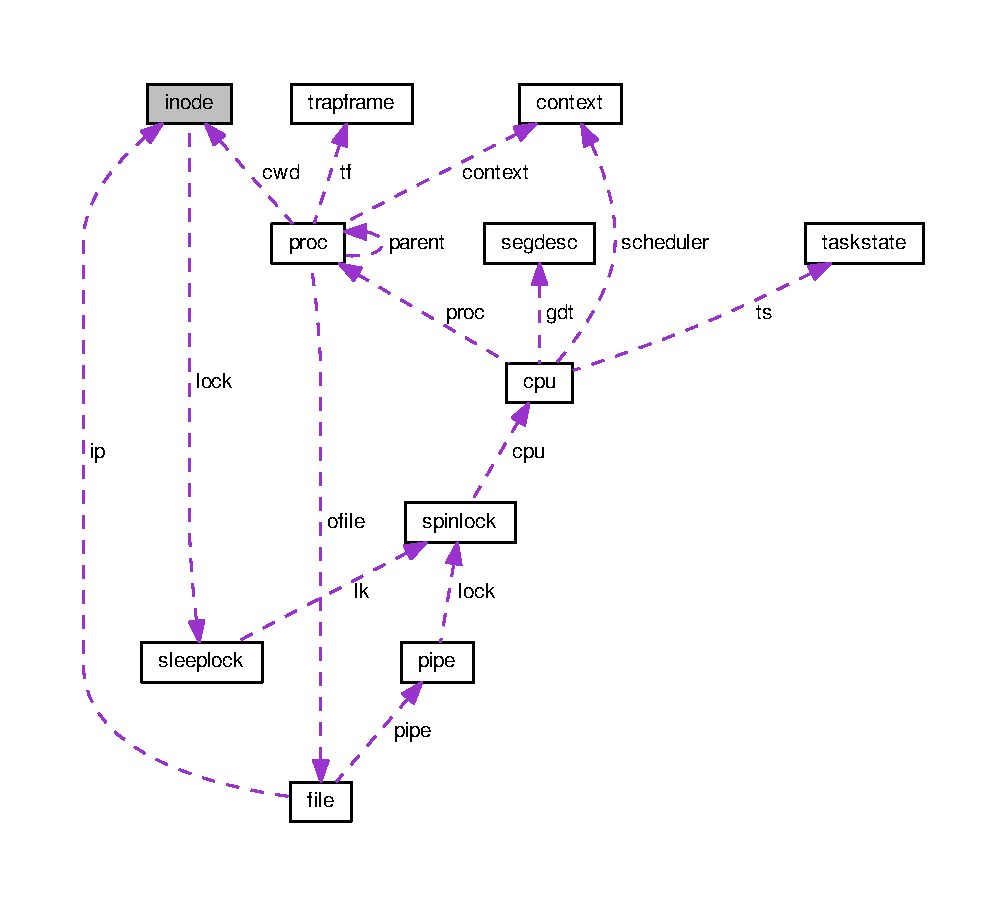
\includegraphics[width=350pt]{d7/d2b/structinode__coll__graph}
\end{center}
\end{figure}
\subsection*{Public Attributes}
\begin{DoxyCompactItemize}
\item 
\hyperlink{types_8h_a91ad9478d81a7aaf2593e8d9c3d06a14}{uint} \hyperlink{structinode_a121742a89c4531f03a7de1613d5be605}{dev}
\item 
\hyperlink{types_8h_a91ad9478d81a7aaf2593e8d9c3d06a14}{uint} \hyperlink{structinode_a8acc2b9df0bfc6856da62925763db7fe}{inum}
\item 
int \hyperlink{structinode_a6a519028ee67f805482b3e1725bf09c5}{ref}
\item 
struct \hyperlink{structsleeplock}{sleeplock} \hyperlink{structinode_a46bad0e938fbd348ac02bdef0c8d6215}{lock}
\item 
int \hyperlink{structinode_aad324382ba30eb83daa5304fce7dca08}{valid}
\item 
short \hyperlink{structinode_a8d74bec2898785c057111c328d23fda2}{type}
\item 
short \hyperlink{structinode_a34af7242018a977dace5730683850875}{major}
\item 
short \hyperlink{structinode_a37878866e7905b666db2aa33076076a2}{minor}
\item 
short \hyperlink{structinode_af8b88b409bea7ef99c49a55f387538b2}{nlink}
\item 
\hyperlink{types_8h_a91ad9478d81a7aaf2593e8d9c3d06a14}{uint} \hyperlink{structinode_a918af769c48a8ca8afac057bf83d12de}{size}
\item 
\hyperlink{types_8h_a91ad9478d81a7aaf2593e8d9c3d06a14}{uint} \hyperlink{structinode_a7ba4ab7e52404b80d6d854678715ae30}{addrs} \mbox{[}\hyperlink{fs_8h_acd38e9532d4b3623f844b93c012a8e06}{N\+D\+I\+R\+E\+CT}+1\mbox{]}
\end{DoxyCompactItemize}


\subsection{Member Data Documentation}
\index{inode@{inode}!addrs@{addrs}}
\index{addrs@{addrs}!inode@{inode}}
\subsubsection[{\texorpdfstring{addrs}{addrs}}]{\setlength{\rightskip}{0pt plus 5cm}{\bf uint} inode\+::addrs\mbox{[}{\bf N\+D\+I\+R\+E\+CT}+1\mbox{]}}\hypertarget{structinode_a7ba4ab7e52404b80d6d854678715ae30}{}\label{structinode_a7ba4ab7e52404b80d6d854678715ae30}
\index{inode@{inode}!dev@{dev}}
\index{dev@{dev}!inode@{inode}}
\subsubsection[{\texorpdfstring{dev}{dev}}]{\setlength{\rightskip}{0pt plus 5cm}{\bf uint} inode\+::dev}\hypertarget{structinode_a121742a89c4531f03a7de1613d5be605}{}\label{structinode_a121742a89c4531f03a7de1613d5be605}
\index{inode@{inode}!inum@{inum}}
\index{inum@{inum}!inode@{inode}}
\subsubsection[{\texorpdfstring{inum}{inum}}]{\setlength{\rightskip}{0pt plus 5cm}{\bf uint} inode\+::inum}\hypertarget{structinode_a8acc2b9df0bfc6856da62925763db7fe}{}\label{structinode_a8acc2b9df0bfc6856da62925763db7fe}
\index{inode@{inode}!lock@{lock}}
\index{lock@{lock}!inode@{inode}}
\subsubsection[{\texorpdfstring{lock}{lock}}]{\setlength{\rightskip}{0pt plus 5cm}struct {\bf sleeplock} inode\+::lock}\hypertarget{structinode_a46bad0e938fbd348ac02bdef0c8d6215}{}\label{structinode_a46bad0e938fbd348ac02bdef0c8d6215}
\index{inode@{inode}!major@{major}}
\index{major@{major}!inode@{inode}}
\subsubsection[{\texorpdfstring{major}{major}}]{\setlength{\rightskip}{0pt plus 5cm}short inode\+::major}\hypertarget{structinode_a34af7242018a977dace5730683850875}{}\label{structinode_a34af7242018a977dace5730683850875}
\index{inode@{inode}!minor@{minor}}
\index{minor@{minor}!inode@{inode}}
\subsubsection[{\texorpdfstring{minor}{minor}}]{\setlength{\rightskip}{0pt plus 5cm}short inode\+::minor}\hypertarget{structinode_a37878866e7905b666db2aa33076076a2}{}\label{structinode_a37878866e7905b666db2aa33076076a2}
\index{inode@{inode}!nlink@{nlink}}
\index{nlink@{nlink}!inode@{inode}}
\subsubsection[{\texorpdfstring{nlink}{nlink}}]{\setlength{\rightskip}{0pt plus 5cm}short inode\+::nlink}\hypertarget{structinode_af8b88b409bea7ef99c49a55f387538b2}{}\label{structinode_af8b88b409bea7ef99c49a55f387538b2}
\index{inode@{inode}!ref@{ref}}
\index{ref@{ref}!inode@{inode}}
\subsubsection[{\texorpdfstring{ref}{ref}}]{\setlength{\rightskip}{0pt plus 5cm}int inode\+::ref}\hypertarget{structinode_a6a519028ee67f805482b3e1725bf09c5}{}\label{structinode_a6a519028ee67f805482b3e1725bf09c5}
\index{inode@{inode}!size@{size}}
\index{size@{size}!inode@{inode}}
\subsubsection[{\texorpdfstring{size}{size}}]{\setlength{\rightskip}{0pt plus 5cm}{\bf uint} inode\+::size}\hypertarget{structinode_a918af769c48a8ca8afac057bf83d12de}{}\label{structinode_a918af769c48a8ca8afac057bf83d12de}
\index{inode@{inode}!type@{type}}
\index{type@{type}!inode@{inode}}
\subsubsection[{\texorpdfstring{type}{type}}]{\setlength{\rightskip}{0pt plus 5cm}short inode\+::type}\hypertarget{structinode_a8d74bec2898785c057111c328d23fda2}{}\label{structinode_a8d74bec2898785c057111c328d23fda2}
\index{inode@{inode}!valid@{valid}}
\index{valid@{valid}!inode@{inode}}
\subsubsection[{\texorpdfstring{valid}{valid}}]{\setlength{\rightskip}{0pt plus 5cm}int inode\+::valid}\hypertarget{structinode_aad324382ba30eb83daa5304fce7dca08}{}\label{structinode_aad324382ba30eb83daa5304fce7dca08}


The documentation for this struct was generated from the following file\+:\begin{DoxyCompactItemize}
\item 
\hyperlink{file_8h}{file.\+h}\end{DoxyCompactItemize}

\hypertarget{structioapic}{}\section{ioapic Struct Reference}
\label{structioapic}\index{ioapic@{ioapic}}
\subsection*{Public Attributes}
\begin{DoxyCompactItemize}
\item 
\hyperlink{types_8h_a91ad9478d81a7aaf2593e8d9c3d06a14}{uint} \hyperlink{structioapic_a84bff406f77801bd1574b9cfb8c23ecf}{reg}
\item 
\hyperlink{types_8h_a91ad9478d81a7aaf2593e8d9c3d06a14}{uint} \hyperlink{structioapic_a28ee224d088b53995504eae8cc8fd6ba}{pad} \mbox{[}3\mbox{]}
\item 
\hyperlink{types_8h_a91ad9478d81a7aaf2593e8d9c3d06a14}{uint} \hyperlink{structioapic_a0612c6bb75dc56f0c4c91ad214a02b3a}{data}
\end{DoxyCompactItemize}


\subsection{Member Data Documentation}
\index{ioapic@{ioapic}!data@{data}}
\index{data@{data}!ioapic@{ioapic}}
\subsubsection[{\texorpdfstring{data}{data}}]{\setlength{\rightskip}{0pt plus 5cm}{\bf uint} ioapic\+::data}\hypertarget{structioapic_a0612c6bb75dc56f0c4c91ad214a02b3a}{}\label{structioapic_a0612c6bb75dc56f0c4c91ad214a02b3a}
\index{ioapic@{ioapic}!pad@{pad}}
\index{pad@{pad}!ioapic@{ioapic}}
\subsubsection[{\texorpdfstring{pad}{pad}}]{\setlength{\rightskip}{0pt plus 5cm}{\bf uint} ioapic\+::pad\mbox{[}3\mbox{]}}\hypertarget{structioapic_a28ee224d088b53995504eae8cc8fd6ba}{}\label{structioapic_a28ee224d088b53995504eae8cc8fd6ba}
\index{ioapic@{ioapic}!reg@{reg}}
\index{reg@{reg}!ioapic@{ioapic}}
\subsubsection[{\texorpdfstring{reg}{reg}}]{\setlength{\rightskip}{0pt plus 5cm}{\bf uint} ioapic\+::reg}\hypertarget{structioapic_a84bff406f77801bd1574b9cfb8c23ecf}{}\label{structioapic_a84bff406f77801bd1574b9cfb8c23ecf}


The documentation for this struct was generated from the following file\+:\begin{DoxyCompactItemize}
\item 
\hyperlink{ioapic_8c}{ioapic.\+c}\end{DoxyCompactItemize}

\hypertarget{structlog}{}\section{log Struct Reference}
\label{structlog}\index{log@{log}}


Collaboration diagram for log\+:\nopagebreak
\begin{figure}[H]
\begin{center}
\leavevmode
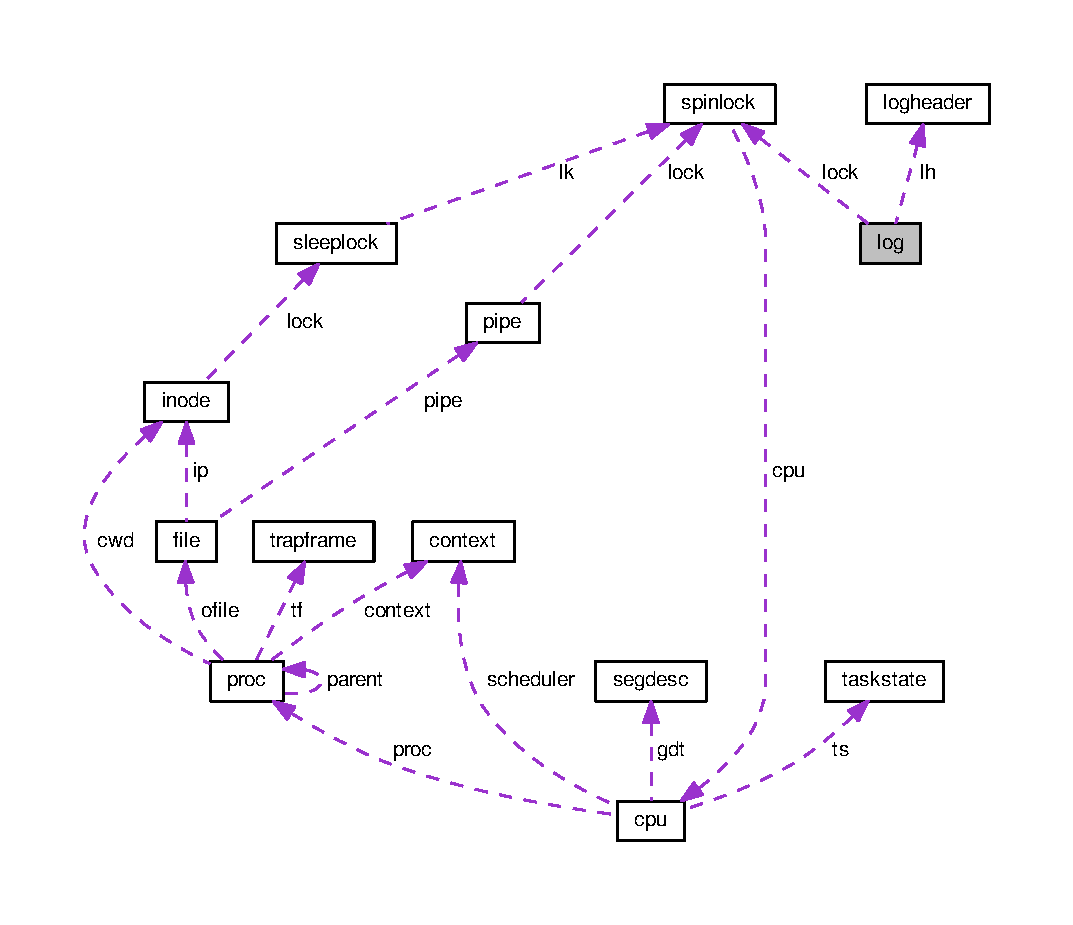
\includegraphics[width=350pt]{d4/d63/structlog__coll__graph}
\end{center}
\end{figure}
\subsection*{Public Attributes}
\begin{DoxyCompactItemize}
\item 
struct \hyperlink{structspinlock}{spinlock} \hyperlink{structlog_a980a1d1aa9c60af7a82f297f8ab54d2e}{lock}
\item 
int \hyperlink{structlog_a28d847dd722497fa3497b14f68267618}{start}
\item 
int \hyperlink{structlog_a2257e716d4b77efd0524286cf5772a41}{size}
\item 
int \hyperlink{structlog_addfc1fc09a124978bd7e2a23a19d733d}{outstanding}
\item 
int \hyperlink{structlog_afc034b98b98897c179ca8fae8e2ee181}{committing}
\item 
int \hyperlink{structlog_aebeeb9df7326549fb5d8b7221c9b0aa3}{dev}
\item 
struct \hyperlink{structlogheader}{logheader} \hyperlink{structlog_a7808516ed2f708dcb13912b1e8fc20d9}{lh}
\end{DoxyCompactItemize}


\subsection{Member Data Documentation}
\index{log@{log}!committing@{committing}}
\index{committing@{committing}!log@{log}}
\subsubsection[{\texorpdfstring{committing}{committing}}]{\setlength{\rightskip}{0pt plus 5cm}int log\+::committing}\hypertarget{structlog_afc034b98b98897c179ca8fae8e2ee181}{}\label{structlog_afc034b98b98897c179ca8fae8e2ee181}
\index{log@{log}!dev@{dev}}
\index{dev@{dev}!log@{log}}
\subsubsection[{\texorpdfstring{dev}{dev}}]{\setlength{\rightskip}{0pt plus 5cm}int log\+::dev}\hypertarget{structlog_aebeeb9df7326549fb5d8b7221c9b0aa3}{}\label{structlog_aebeeb9df7326549fb5d8b7221c9b0aa3}
\index{log@{log}!lh@{lh}}
\index{lh@{lh}!log@{log}}
\subsubsection[{\texorpdfstring{lh}{lh}}]{\setlength{\rightskip}{0pt plus 5cm}struct {\bf logheader} log\+::lh}\hypertarget{structlog_a7808516ed2f708dcb13912b1e8fc20d9}{}\label{structlog_a7808516ed2f708dcb13912b1e8fc20d9}
\index{log@{log}!lock@{lock}}
\index{lock@{lock}!log@{log}}
\subsubsection[{\texorpdfstring{lock}{lock}}]{\setlength{\rightskip}{0pt plus 5cm}struct {\bf spinlock} log\+::lock}\hypertarget{structlog_a980a1d1aa9c60af7a82f297f8ab54d2e}{}\label{structlog_a980a1d1aa9c60af7a82f297f8ab54d2e}
\index{log@{log}!outstanding@{outstanding}}
\index{outstanding@{outstanding}!log@{log}}
\subsubsection[{\texorpdfstring{outstanding}{outstanding}}]{\setlength{\rightskip}{0pt plus 5cm}int log\+::outstanding}\hypertarget{structlog_addfc1fc09a124978bd7e2a23a19d733d}{}\label{structlog_addfc1fc09a124978bd7e2a23a19d733d}
\index{log@{log}!size@{size}}
\index{size@{size}!log@{log}}
\subsubsection[{\texorpdfstring{size}{size}}]{\setlength{\rightskip}{0pt plus 5cm}int log\+::size}\hypertarget{structlog_a2257e716d4b77efd0524286cf5772a41}{}\label{structlog_a2257e716d4b77efd0524286cf5772a41}
\index{log@{log}!start@{start}}
\index{start@{start}!log@{log}}
\subsubsection[{\texorpdfstring{start}{start}}]{\setlength{\rightskip}{0pt plus 5cm}int log\+::start}\hypertarget{structlog_a28d847dd722497fa3497b14f68267618}{}\label{structlog_a28d847dd722497fa3497b14f68267618}


The documentation for this struct was generated from the following file\+:\begin{DoxyCompactItemize}
\item 
\hyperlink{log_8c}{log.\+c}\end{DoxyCompactItemize}

\hypertarget{structlogheader}{}\section{logheader Struct Reference}
\label{structlogheader}\index{logheader@{logheader}}
\subsection*{Public Attributes}
\begin{DoxyCompactItemize}
\item 
int \hyperlink{structlogheader_a50b276b70d44ae77497ef1d71d182875}{n}
\item 
int \hyperlink{structlogheader_a020db7fe04c7ce6b8f4aee2092576c2c}{block} \mbox{[}\hyperlink{param_8h_acc7694167c7840a913939a1b90808b4c}{L\+O\+G\+S\+I\+ZE}\mbox{]}
\end{DoxyCompactItemize}


\subsection{Member Data Documentation}
\index{logheader@{logheader}!block@{block}}
\index{block@{block}!logheader@{logheader}}
\subsubsection[{\texorpdfstring{block}{block}}]{\setlength{\rightskip}{0pt plus 5cm}int logheader\+::block\mbox{[}{\bf L\+O\+G\+S\+I\+ZE}\mbox{]}}\hypertarget{structlogheader_a020db7fe04c7ce6b8f4aee2092576c2c}{}\label{structlogheader_a020db7fe04c7ce6b8f4aee2092576c2c}
\index{logheader@{logheader}!n@{n}}
\index{n@{n}!logheader@{logheader}}
\subsubsection[{\texorpdfstring{n}{n}}]{\setlength{\rightskip}{0pt plus 5cm}int logheader\+::n}\hypertarget{structlogheader_a50b276b70d44ae77497ef1d71d182875}{}\label{structlogheader_a50b276b70d44ae77497ef1d71d182875}


The documentation for this struct was generated from the following file\+:\begin{DoxyCompactItemize}
\item 
\hyperlink{log_8c}{log.\+c}\end{DoxyCompactItemize}

\hypertarget{structmp}{}\section{mp Struct Reference}
\label{structmp}\index{mp@{mp}}


{\ttfamily \#include $<$mp.\+h$>$}

\subsection*{Public Attributes}
\begin{DoxyCompactItemize}
\item 
\hyperlink{types_8h_a65f85814a8290f9797005d3b28e7e5fc}{uchar} \hyperlink{structmp_af2bfc400b8e6edae4c0e6ff437a2a1f4}{signature} \mbox{[}4\mbox{]}
\item 
void $\ast$ \hyperlink{structmp_a3333bff25a42470efb69b3b01f08d6ce}{physaddr}
\item 
\hyperlink{types_8h_a65f85814a8290f9797005d3b28e7e5fc}{uchar} \hyperlink{structmp_a46a03e7ef27f7290a5fb49bcb4c3c507}{length}
\item 
\hyperlink{types_8h_a65f85814a8290f9797005d3b28e7e5fc}{uchar} \hyperlink{structmp_a0be99b736e3c6fb1f405944868674063}{specrev}
\item 
\hyperlink{types_8h_a65f85814a8290f9797005d3b28e7e5fc}{uchar} \hyperlink{structmp_a0d403ddb2898b8cadf31f9f75d31163a}{checksum}
\item 
\hyperlink{types_8h_a65f85814a8290f9797005d3b28e7e5fc}{uchar} \hyperlink{structmp_a08cf79f94b4dcfce588ccb41f90cbe0e}{type}
\item 
\hyperlink{types_8h_a65f85814a8290f9797005d3b28e7e5fc}{uchar} \hyperlink{structmp_ae2157bc407a7423c57bdb078b70cd6e5}{imcrp}
\item 
\hyperlink{types_8h_a65f85814a8290f9797005d3b28e7e5fc}{uchar} \hyperlink{structmp_a7a87ebdff0db6123f294d93ee98c42ab}{reserved} \mbox{[}3\mbox{]}
\end{DoxyCompactItemize}


\subsection{Member Data Documentation}
\index{mp@{mp}!checksum@{checksum}}
\index{checksum@{checksum}!mp@{mp}}
\subsubsection[{\texorpdfstring{checksum}{checksum}}]{\setlength{\rightskip}{0pt plus 5cm}{\bf uchar} mp\+::checksum}\hypertarget{structmp_a0d403ddb2898b8cadf31f9f75d31163a}{}\label{structmp_a0d403ddb2898b8cadf31f9f75d31163a}
\index{mp@{mp}!imcrp@{imcrp}}
\index{imcrp@{imcrp}!mp@{mp}}
\subsubsection[{\texorpdfstring{imcrp}{imcrp}}]{\setlength{\rightskip}{0pt plus 5cm}{\bf uchar} mp\+::imcrp}\hypertarget{structmp_ae2157bc407a7423c57bdb078b70cd6e5}{}\label{structmp_ae2157bc407a7423c57bdb078b70cd6e5}
\index{mp@{mp}!length@{length}}
\index{length@{length}!mp@{mp}}
\subsubsection[{\texorpdfstring{length}{length}}]{\setlength{\rightskip}{0pt plus 5cm}{\bf uchar} mp\+::length}\hypertarget{structmp_a46a03e7ef27f7290a5fb49bcb4c3c507}{}\label{structmp_a46a03e7ef27f7290a5fb49bcb4c3c507}
\index{mp@{mp}!physaddr@{physaddr}}
\index{physaddr@{physaddr}!mp@{mp}}
\subsubsection[{\texorpdfstring{physaddr}{physaddr}}]{\setlength{\rightskip}{0pt plus 5cm}void$\ast$ mp\+::physaddr}\hypertarget{structmp_a3333bff25a42470efb69b3b01f08d6ce}{}\label{structmp_a3333bff25a42470efb69b3b01f08d6ce}
\index{mp@{mp}!reserved@{reserved}}
\index{reserved@{reserved}!mp@{mp}}
\subsubsection[{\texorpdfstring{reserved}{reserved}}]{\setlength{\rightskip}{0pt plus 5cm}{\bf uchar} mp\+::reserved\mbox{[}3\mbox{]}}\hypertarget{structmp_a7a87ebdff0db6123f294d93ee98c42ab}{}\label{structmp_a7a87ebdff0db6123f294d93ee98c42ab}
\index{mp@{mp}!signature@{signature}}
\index{signature@{signature}!mp@{mp}}
\subsubsection[{\texorpdfstring{signature}{signature}}]{\setlength{\rightskip}{0pt plus 5cm}{\bf uchar} mp\+::signature\mbox{[}4\mbox{]}}\hypertarget{structmp_af2bfc400b8e6edae4c0e6ff437a2a1f4}{}\label{structmp_af2bfc400b8e6edae4c0e6ff437a2a1f4}
\index{mp@{mp}!specrev@{specrev}}
\index{specrev@{specrev}!mp@{mp}}
\subsubsection[{\texorpdfstring{specrev}{specrev}}]{\setlength{\rightskip}{0pt plus 5cm}{\bf uchar} mp\+::specrev}\hypertarget{structmp_a0be99b736e3c6fb1f405944868674063}{}\label{structmp_a0be99b736e3c6fb1f405944868674063}
\index{mp@{mp}!type@{type}}
\index{type@{type}!mp@{mp}}
\subsubsection[{\texorpdfstring{type}{type}}]{\setlength{\rightskip}{0pt plus 5cm}{\bf uchar} mp\+::type}\hypertarget{structmp_a08cf79f94b4dcfce588ccb41f90cbe0e}{}\label{structmp_a08cf79f94b4dcfce588ccb41f90cbe0e}


The documentation for this struct was generated from the following file\+:\begin{DoxyCompactItemize}
\item 
\hyperlink{mp_8h}{mp.\+h}\end{DoxyCompactItemize}

\hypertarget{structmpconf}{}\section{mpconf Struct Reference}
\label{structmpconf}\index{mpconf@{mpconf}}


{\ttfamily \#include $<$mp.\+h$>$}

\subsection*{Public Attributes}
\begin{DoxyCompactItemize}
\item 
\hyperlink{types_8h_a65f85814a8290f9797005d3b28e7e5fc}{uchar} \hyperlink{structmpconf_a7bf26b6b2b09d4265ffcbdb362bc5c8b}{signature} \mbox{[}4\mbox{]}
\item 
\hyperlink{types_8h_ab95f123a6c9bcfee6a343170ef8c5f69}{ushort} \hyperlink{structmpconf_a6b7583180c78b6a2e490d6c72779d8dd}{length}
\item 
\hyperlink{types_8h_a65f85814a8290f9797005d3b28e7e5fc}{uchar} \hyperlink{structmpconf_ade1055584605c76f4e1134d6631e0afa}{version}
\item 
\hyperlink{types_8h_a65f85814a8290f9797005d3b28e7e5fc}{uchar} \hyperlink{structmpconf_aac54c4c7710b90574416a945cdcd3b9e}{checksum}
\item 
\hyperlink{types_8h_a65f85814a8290f9797005d3b28e7e5fc}{uchar} \hyperlink{structmpconf_ac4e4d4d150aac8ea0bba92ff2cfae557}{product} \mbox{[}20\mbox{]}
\item 
\hyperlink{types_8h_a91ad9478d81a7aaf2593e8d9c3d06a14}{uint} $\ast$ \hyperlink{structmpconf_a1b3e44d3639e8f3117e6bca9626d680b}{oemtable}
\item 
\hyperlink{types_8h_ab95f123a6c9bcfee6a343170ef8c5f69}{ushort} \hyperlink{structmpconf_a5aaf9c7afa2f1be645b8e633f6ff43a1}{oemlength}
\item 
\hyperlink{types_8h_ab95f123a6c9bcfee6a343170ef8c5f69}{ushort} \hyperlink{structmpconf_a75f67295a180d1f72b93be82e09ecc2a}{entry}
\item 
\hyperlink{types_8h_a91ad9478d81a7aaf2593e8d9c3d06a14}{uint} $\ast$ \hyperlink{structmpconf_a087fac7e9dc4ca1fdfe142b3adf96c99}{lapicaddr}
\item 
\hyperlink{types_8h_ab95f123a6c9bcfee6a343170ef8c5f69}{ushort} \hyperlink{structmpconf_adbda8ec5a43970662e7eab8f8da11817}{xlength}
\item 
\hyperlink{types_8h_a65f85814a8290f9797005d3b28e7e5fc}{uchar} \hyperlink{structmpconf_a499447fb50cb158a848f66f124dd8f8d}{xchecksum}
\item 
\hyperlink{types_8h_a65f85814a8290f9797005d3b28e7e5fc}{uchar} \hyperlink{structmpconf_ab7ce4c5b90a538f41baefef6714d1a23}{reserved}
\end{DoxyCompactItemize}


\subsection{Member Data Documentation}
\index{mpconf@{mpconf}!checksum@{checksum}}
\index{checksum@{checksum}!mpconf@{mpconf}}
\subsubsection[{\texorpdfstring{checksum}{checksum}}]{\setlength{\rightskip}{0pt plus 5cm}{\bf uchar} mpconf\+::checksum}\hypertarget{structmpconf_aac54c4c7710b90574416a945cdcd3b9e}{}\label{structmpconf_aac54c4c7710b90574416a945cdcd3b9e}
\index{mpconf@{mpconf}!entry@{entry}}
\index{entry@{entry}!mpconf@{mpconf}}
\subsubsection[{\texorpdfstring{entry}{entry}}]{\setlength{\rightskip}{0pt plus 5cm}{\bf ushort} mpconf\+::entry}\hypertarget{structmpconf_a75f67295a180d1f72b93be82e09ecc2a}{}\label{structmpconf_a75f67295a180d1f72b93be82e09ecc2a}
\index{mpconf@{mpconf}!lapicaddr@{lapicaddr}}
\index{lapicaddr@{lapicaddr}!mpconf@{mpconf}}
\subsubsection[{\texorpdfstring{lapicaddr}{lapicaddr}}]{\setlength{\rightskip}{0pt plus 5cm}{\bf uint}$\ast$ mpconf\+::lapicaddr}\hypertarget{structmpconf_a087fac7e9dc4ca1fdfe142b3adf96c99}{}\label{structmpconf_a087fac7e9dc4ca1fdfe142b3adf96c99}
\index{mpconf@{mpconf}!length@{length}}
\index{length@{length}!mpconf@{mpconf}}
\subsubsection[{\texorpdfstring{length}{length}}]{\setlength{\rightskip}{0pt plus 5cm}{\bf ushort} mpconf\+::length}\hypertarget{structmpconf_a6b7583180c78b6a2e490d6c72779d8dd}{}\label{structmpconf_a6b7583180c78b6a2e490d6c72779d8dd}
\index{mpconf@{mpconf}!oemlength@{oemlength}}
\index{oemlength@{oemlength}!mpconf@{mpconf}}
\subsubsection[{\texorpdfstring{oemlength}{oemlength}}]{\setlength{\rightskip}{0pt plus 5cm}{\bf ushort} mpconf\+::oemlength}\hypertarget{structmpconf_a5aaf9c7afa2f1be645b8e633f6ff43a1}{}\label{structmpconf_a5aaf9c7afa2f1be645b8e633f6ff43a1}
\index{mpconf@{mpconf}!oemtable@{oemtable}}
\index{oemtable@{oemtable}!mpconf@{mpconf}}
\subsubsection[{\texorpdfstring{oemtable}{oemtable}}]{\setlength{\rightskip}{0pt plus 5cm}{\bf uint}$\ast$ mpconf\+::oemtable}\hypertarget{structmpconf_a1b3e44d3639e8f3117e6bca9626d680b}{}\label{structmpconf_a1b3e44d3639e8f3117e6bca9626d680b}
\index{mpconf@{mpconf}!product@{product}}
\index{product@{product}!mpconf@{mpconf}}
\subsubsection[{\texorpdfstring{product}{product}}]{\setlength{\rightskip}{0pt plus 5cm}{\bf uchar} mpconf\+::product\mbox{[}20\mbox{]}}\hypertarget{structmpconf_ac4e4d4d150aac8ea0bba92ff2cfae557}{}\label{structmpconf_ac4e4d4d150aac8ea0bba92ff2cfae557}
\index{mpconf@{mpconf}!reserved@{reserved}}
\index{reserved@{reserved}!mpconf@{mpconf}}
\subsubsection[{\texorpdfstring{reserved}{reserved}}]{\setlength{\rightskip}{0pt plus 5cm}{\bf uchar} mpconf\+::reserved}\hypertarget{structmpconf_ab7ce4c5b90a538f41baefef6714d1a23}{}\label{structmpconf_ab7ce4c5b90a538f41baefef6714d1a23}
\index{mpconf@{mpconf}!signature@{signature}}
\index{signature@{signature}!mpconf@{mpconf}}
\subsubsection[{\texorpdfstring{signature}{signature}}]{\setlength{\rightskip}{0pt plus 5cm}{\bf uchar} mpconf\+::signature\mbox{[}4\mbox{]}}\hypertarget{structmpconf_a7bf26b6b2b09d4265ffcbdb362bc5c8b}{}\label{structmpconf_a7bf26b6b2b09d4265ffcbdb362bc5c8b}
\index{mpconf@{mpconf}!version@{version}}
\index{version@{version}!mpconf@{mpconf}}
\subsubsection[{\texorpdfstring{version}{version}}]{\setlength{\rightskip}{0pt plus 5cm}{\bf uchar} mpconf\+::version}\hypertarget{structmpconf_ade1055584605c76f4e1134d6631e0afa}{}\label{structmpconf_ade1055584605c76f4e1134d6631e0afa}
\index{mpconf@{mpconf}!xchecksum@{xchecksum}}
\index{xchecksum@{xchecksum}!mpconf@{mpconf}}
\subsubsection[{\texorpdfstring{xchecksum}{xchecksum}}]{\setlength{\rightskip}{0pt plus 5cm}{\bf uchar} mpconf\+::xchecksum}\hypertarget{structmpconf_a499447fb50cb158a848f66f124dd8f8d}{}\label{structmpconf_a499447fb50cb158a848f66f124dd8f8d}
\index{mpconf@{mpconf}!xlength@{xlength}}
\index{xlength@{xlength}!mpconf@{mpconf}}
\subsubsection[{\texorpdfstring{xlength}{xlength}}]{\setlength{\rightskip}{0pt plus 5cm}{\bf ushort} mpconf\+::xlength}\hypertarget{structmpconf_adbda8ec5a43970662e7eab8f8da11817}{}\label{structmpconf_adbda8ec5a43970662e7eab8f8da11817}


The documentation for this struct was generated from the following file\+:\begin{DoxyCompactItemize}
\item 
\hyperlink{mp_8h}{mp.\+h}\end{DoxyCompactItemize}

\hypertarget{structmpioapic}{}\section{mpioapic Struct Reference}
\label{structmpioapic}\index{mpioapic@{mpioapic}}


{\ttfamily \#include $<$mp.\+h$>$}

\subsection*{Public Attributes}
\begin{DoxyCompactItemize}
\item 
\hyperlink{types_8h_a65f85814a8290f9797005d3b28e7e5fc}{uchar} \hyperlink{structmpioapic_a8d7527bad798d6f8a59a21df06879f0f}{type}
\item 
\hyperlink{types_8h_a65f85814a8290f9797005d3b28e7e5fc}{uchar} \hyperlink{structmpioapic_a9a975b41f6af43937d67c3b63235dd7d}{apicno}
\item 
\hyperlink{types_8h_a65f85814a8290f9797005d3b28e7e5fc}{uchar} \hyperlink{structmpioapic_a7c6f3d950f89e2b982fd53f7c59681e7}{version}
\item 
\hyperlink{types_8h_a65f85814a8290f9797005d3b28e7e5fc}{uchar} \hyperlink{structmpioapic_a9cc0f4c76312b7d074c558cbcad38a12}{flags}
\item 
\hyperlink{types_8h_a91ad9478d81a7aaf2593e8d9c3d06a14}{uint} $\ast$ \hyperlink{structmpioapic_a364bbba1df7846f9c6d271c7c85a7aaa}{addr}
\end{DoxyCompactItemize}


\subsection{Member Data Documentation}
\index{mpioapic@{mpioapic}!addr@{addr}}
\index{addr@{addr}!mpioapic@{mpioapic}}
\subsubsection[{\texorpdfstring{addr}{addr}}]{\setlength{\rightskip}{0pt plus 5cm}{\bf uint}$\ast$ mpioapic\+::addr}\hypertarget{structmpioapic_a364bbba1df7846f9c6d271c7c85a7aaa}{}\label{structmpioapic_a364bbba1df7846f9c6d271c7c85a7aaa}
\index{mpioapic@{mpioapic}!apicno@{apicno}}
\index{apicno@{apicno}!mpioapic@{mpioapic}}
\subsubsection[{\texorpdfstring{apicno}{apicno}}]{\setlength{\rightskip}{0pt plus 5cm}{\bf uchar} mpioapic\+::apicno}\hypertarget{structmpioapic_a9a975b41f6af43937d67c3b63235dd7d}{}\label{structmpioapic_a9a975b41f6af43937d67c3b63235dd7d}
\index{mpioapic@{mpioapic}!flags@{flags}}
\index{flags@{flags}!mpioapic@{mpioapic}}
\subsubsection[{\texorpdfstring{flags}{flags}}]{\setlength{\rightskip}{0pt plus 5cm}{\bf uchar} mpioapic\+::flags}\hypertarget{structmpioapic_a9cc0f4c76312b7d074c558cbcad38a12}{}\label{structmpioapic_a9cc0f4c76312b7d074c558cbcad38a12}
\index{mpioapic@{mpioapic}!type@{type}}
\index{type@{type}!mpioapic@{mpioapic}}
\subsubsection[{\texorpdfstring{type}{type}}]{\setlength{\rightskip}{0pt plus 5cm}{\bf uchar} mpioapic\+::type}\hypertarget{structmpioapic_a8d7527bad798d6f8a59a21df06879f0f}{}\label{structmpioapic_a8d7527bad798d6f8a59a21df06879f0f}
\index{mpioapic@{mpioapic}!version@{version}}
\index{version@{version}!mpioapic@{mpioapic}}
\subsubsection[{\texorpdfstring{version}{version}}]{\setlength{\rightskip}{0pt plus 5cm}{\bf uchar} mpioapic\+::version}\hypertarget{structmpioapic_a7c6f3d950f89e2b982fd53f7c59681e7}{}\label{structmpioapic_a7c6f3d950f89e2b982fd53f7c59681e7}


The documentation for this struct was generated from the following file\+:\begin{DoxyCompactItemize}
\item 
\hyperlink{mp_8h}{mp.\+h}\end{DoxyCompactItemize}

\hypertarget{structmpproc}{}\section{mpproc Struct Reference}
\label{structmpproc}\index{mpproc@{mpproc}}


{\ttfamily \#include $<$mp.\+h$>$}

\subsection*{Public Attributes}
\begin{DoxyCompactItemize}
\item 
\hyperlink{types_8h_a65f85814a8290f9797005d3b28e7e5fc}{uchar} \hyperlink{structmpproc_acd7371100bf5624c8eafe1280826f358}{type}
\item 
\hyperlink{types_8h_a65f85814a8290f9797005d3b28e7e5fc}{uchar} \hyperlink{structmpproc_a935db2a1561da721c867f4b82c51d04d}{apicid}
\item 
\hyperlink{types_8h_a65f85814a8290f9797005d3b28e7e5fc}{uchar} \hyperlink{structmpproc_a6d7948bc046404527c0eec71e3e93209}{version}
\item 
\hyperlink{types_8h_a65f85814a8290f9797005d3b28e7e5fc}{uchar} \hyperlink{structmpproc_abac8cdeb6e601ce8e5bf343c8efb3680}{flags}
\item 
\hyperlink{types_8h_a65f85814a8290f9797005d3b28e7e5fc}{uchar} \hyperlink{structmpproc_a2e18fc2c01b252da2c0d671fdce95eb5}{signature} \mbox{[}4\mbox{]}
\item 
\hyperlink{types_8h_a91ad9478d81a7aaf2593e8d9c3d06a14}{uint} \hyperlink{structmpproc_a62dc15542eee0797a4636b701439b6d9}{feature}
\item 
\hyperlink{types_8h_a65f85814a8290f9797005d3b28e7e5fc}{uchar} \hyperlink{structmpproc_a94bbb1f4794bcf6126fb36520f668134}{reserved} \mbox{[}8\mbox{]}
\end{DoxyCompactItemize}


\subsection{Member Data Documentation}
\index{mpproc@{mpproc}!apicid@{apicid}}
\index{apicid@{apicid}!mpproc@{mpproc}}
\subsubsection[{\texorpdfstring{apicid}{apicid}}]{\setlength{\rightskip}{0pt plus 5cm}{\bf uchar} mpproc\+::apicid}\hypertarget{structmpproc_a935db2a1561da721c867f4b82c51d04d}{}\label{structmpproc_a935db2a1561da721c867f4b82c51d04d}
\index{mpproc@{mpproc}!feature@{feature}}
\index{feature@{feature}!mpproc@{mpproc}}
\subsubsection[{\texorpdfstring{feature}{feature}}]{\setlength{\rightskip}{0pt plus 5cm}{\bf uint} mpproc\+::feature}\hypertarget{structmpproc_a62dc15542eee0797a4636b701439b6d9}{}\label{structmpproc_a62dc15542eee0797a4636b701439b6d9}
\index{mpproc@{mpproc}!flags@{flags}}
\index{flags@{flags}!mpproc@{mpproc}}
\subsubsection[{\texorpdfstring{flags}{flags}}]{\setlength{\rightskip}{0pt plus 5cm}{\bf uchar} mpproc\+::flags}\hypertarget{structmpproc_abac8cdeb6e601ce8e5bf343c8efb3680}{}\label{structmpproc_abac8cdeb6e601ce8e5bf343c8efb3680}
\index{mpproc@{mpproc}!reserved@{reserved}}
\index{reserved@{reserved}!mpproc@{mpproc}}
\subsubsection[{\texorpdfstring{reserved}{reserved}}]{\setlength{\rightskip}{0pt plus 5cm}{\bf uchar} mpproc\+::reserved\mbox{[}8\mbox{]}}\hypertarget{structmpproc_a94bbb1f4794bcf6126fb36520f668134}{}\label{structmpproc_a94bbb1f4794bcf6126fb36520f668134}
\index{mpproc@{mpproc}!signature@{signature}}
\index{signature@{signature}!mpproc@{mpproc}}
\subsubsection[{\texorpdfstring{signature}{signature}}]{\setlength{\rightskip}{0pt plus 5cm}{\bf uchar} mpproc\+::signature\mbox{[}4\mbox{]}}\hypertarget{structmpproc_a2e18fc2c01b252da2c0d671fdce95eb5}{}\label{structmpproc_a2e18fc2c01b252da2c0d671fdce95eb5}
\index{mpproc@{mpproc}!type@{type}}
\index{type@{type}!mpproc@{mpproc}}
\subsubsection[{\texorpdfstring{type}{type}}]{\setlength{\rightskip}{0pt plus 5cm}{\bf uchar} mpproc\+::type}\hypertarget{structmpproc_acd7371100bf5624c8eafe1280826f358}{}\label{structmpproc_acd7371100bf5624c8eafe1280826f358}
\index{mpproc@{mpproc}!version@{version}}
\index{version@{version}!mpproc@{mpproc}}
\subsubsection[{\texorpdfstring{version}{version}}]{\setlength{\rightskip}{0pt plus 5cm}{\bf uchar} mpproc\+::version}\hypertarget{structmpproc_a6d7948bc046404527c0eec71e3e93209}{}\label{structmpproc_a6d7948bc046404527c0eec71e3e93209}


The documentation for this struct was generated from the following file\+:\begin{DoxyCompactItemize}
\item 
\hyperlink{mp_8h}{mp.\+h}\end{DoxyCompactItemize}

\hypertarget{structpipe}{}\section{pipe Struct Reference}
\label{structpipe}\index{pipe@{pipe}}


Collaboration diagram for pipe\+:\nopagebreak
\begin{figure}[H]
\begin{center}
\leavevmode
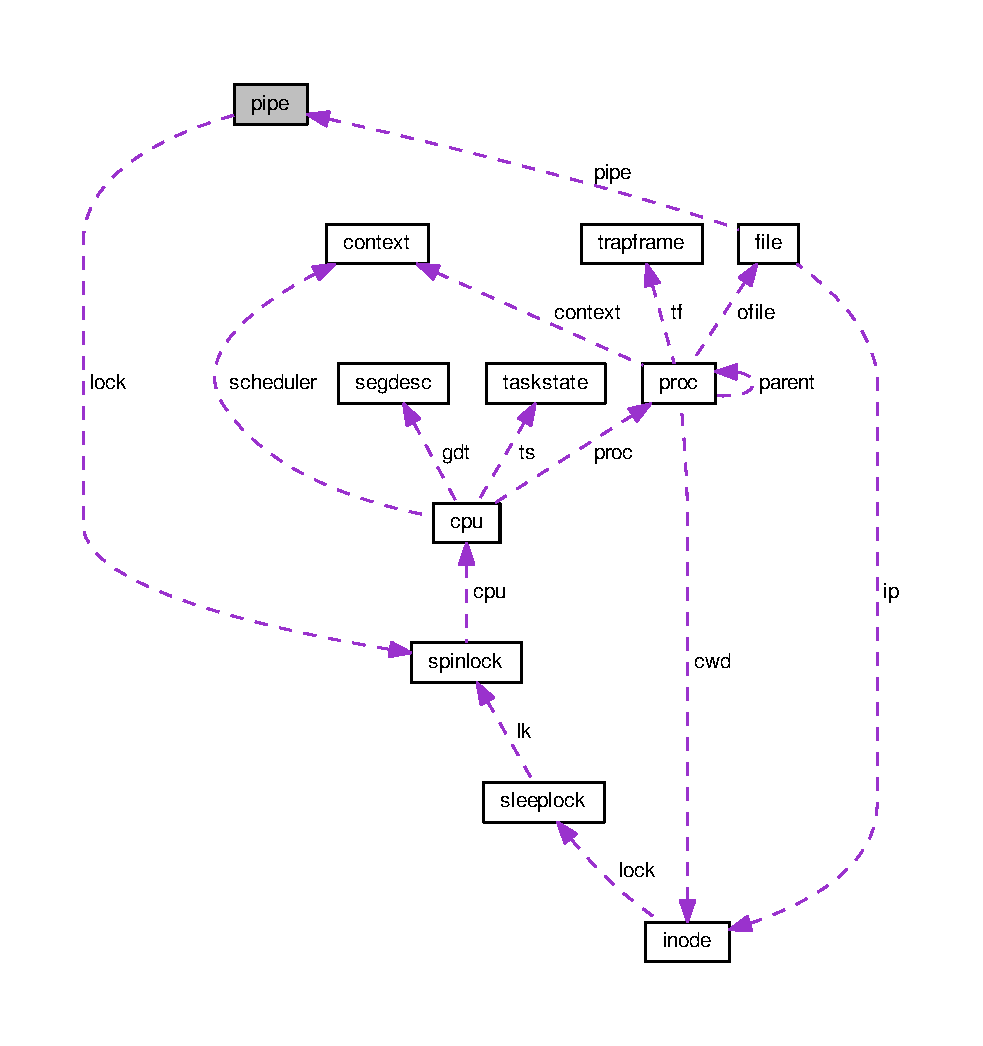
\includegraphics[width=350pt]{df/d8e/structpipe__coll__graph}
\end{center}
\end{figure}
\subsection*{Public Attributes}
\begin{DoxyCompactItemize}
\item 
struct \hyperlink{structspinlock}{spinlock} \hyperlink{structpipe_a0ce399a2ba316d11cb8e678069bfd5b4}{lock}
\item 
char \hyperlink{structpipe_ab02ae9fa0b8b092512c28c7c080f0c7b}{data} \mbox{[}\hyperlink{pipe_8c_ad3dc9214a710d7a6c516cbaa2a12a1de}{P\+I\+P\+E\+S\+I\+ZE}\mbox{]}
\item 
\hyperlink{types_8h_a91ad9478d81a7aaf2593e8d9c3d06a14}{uint} \hyperlink{structpipe_ad71eb56c445f9178dac07ae47f352fd1}{nread}
\item 
\hyperlink{types_8h_a91ad9478d81a7aaf2593e8d9c3d06a14}{uint} \hyperlink{structpipe_a419b6fc2780013358de51c91371dac66}{nwrite}
\item 
int \hyperlink{structpipe_a7bdc57b39ef97dda61e468ad9e8dbfba}{readopen}
\item 
int \hyperlink{structpipe_a9538da698ddd63615c991a318094663b}{writeopen}
\end{DoxyCompactItemize}


\subsection{Member Data Documentation}
\index{pipe@{pipe}!data@{data}}
\index{data@{data}!pipe@{pipe}}
\subsubsection[{\texorpdfstring{data}{data}}]{\setlength{\rightskip}{0pt plus 5cm}char pipe\+::data\mbox{[}{\bf P\+I\+P\+E\+S\+I\+ZE}\mbox{]}}\hypertarget{structpipe_ab02ae9fa0b8b092512c28c7c080f0c7b}{}\label{structpipe_ab02ae9fa0b8b092512c28c7c080f0c7b}
\index{pipe@{pipe}!lock@{lock}}
\index{lock@{lock}!pipe@{pipe}}
\subsubsection[{\texorpdfstring{lock}{lock}}]{\setlength{\rightskip}{0pt plus 5cm}struct {\bf spinlock} pipe\+::lock}\hypertarget{structpipe_a0ce399a2ba316d11cb8e678069bfd5b4}{}\label{structpipe_a0ce399a2ba316d11cb8e678069bfd5b4}
\index{pipe@{pipe}!nread@{nread}}
\index{nread@{nread}!pipe@{pipe}}
\subsubsection[{\texorpdfstring{nread}{nread}}]{\setlength{\rightskip}{0pt plus 5cm}{\bf uint} pipe\+::nread}\hypertarget{structpipe_ad71eb56c445f9178dac07ae47f352fd1}{}\label{structpipe_ad71eb56c445f9178dac07ae47f352fd1}
\index{pipe@{pipe}!nwrite@{nwrite}}
\index{nwrite@{nwrite}!pipe@{pipe}}
\subsubsection[{\texorpdfstring{nwrite}{nwrite}}]{\setlength{\rightskip}{0pt plus 5cm}{\bf uint} pipe\+::nwrite}\hypertarget{structpipe_a419b6fc2780013358de51c91371dac66}{}\label{structpipe_a419b6fc2780013358de51c91371dac66}
\index{pipe@{pipe}!readopen@{readopen}}
\index{readopen@{readopen}!pipe@{pipe}}
\subsubsection[{\texorpdfstring{readopen}{readopen}}]{\setlength{\rightskip}{0pt plus 5cm}int pipe\+::readopen}\hypertarget{structpipe_a7bdc57b39ef97dda61e468ad9e8dbfba}{}\label{structpipe_a7bdc57b39ef97dda61e468ad9e8dbfba}
\index{pipe@{pipe}!writeopen@{writeopen}}
\index{writeopen@{writeopen}!pipe@{pipe}}
\subsubsection[{\texorpdfstring{writeopen}{writeopen}}]{\setlength{\rightskip}{0pt plus 5cm}int pipe\+::writeopen}\hypertarget{structpipe_a9538da698ddd63615c991a318094663b}{}\label{structpipe_a9538da698ddd63615c991a318094663b}


The documentation for this struct was generated from the following file\+:\begin{DoxyCompactItemize}
\item 
\hyperlink{pipe_8c}{pipe.\+c}\end{DoxyCompactItemize}

\hypertarget{structproc}{}\section{proc Struct Reference}
\label{structproc}\index{proc@{proc}}


{\ttfamily \#include $<$proc.\+h$>$}



Collaboration diagram for proc\+:\nopagebreak
\begin{figure}[H]
\begin{center}
\leavevmode
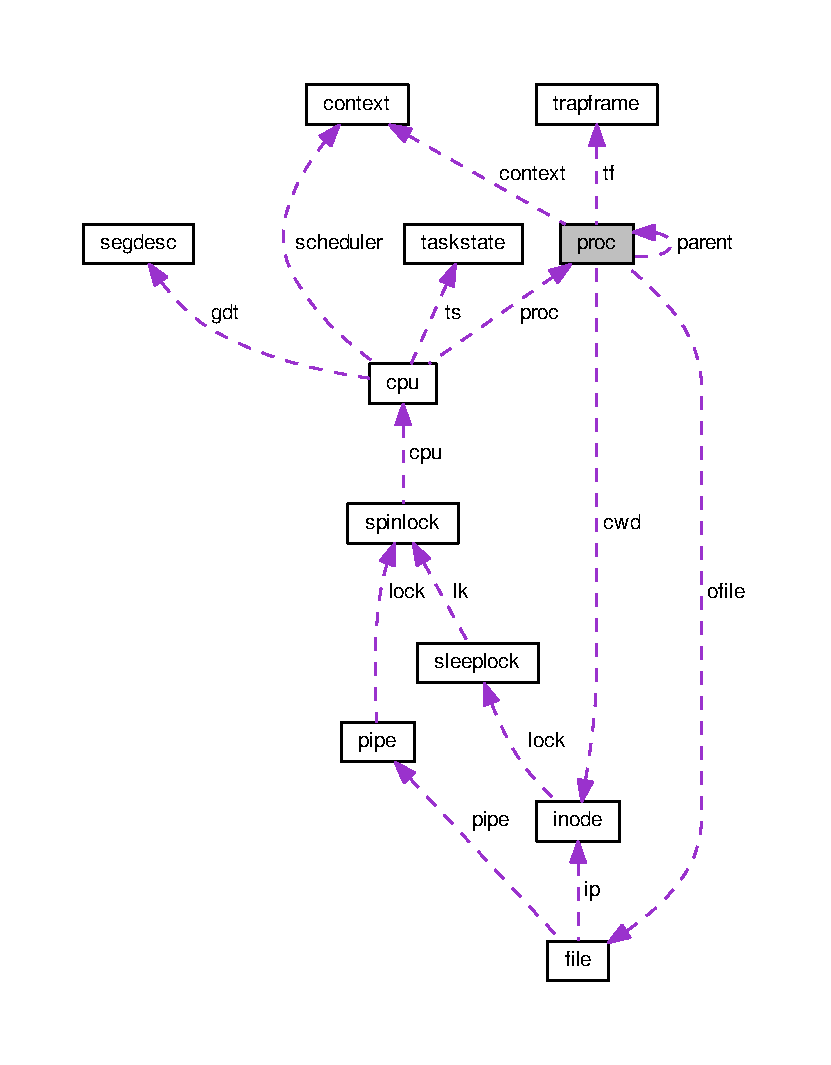
\includegraphics[width=350pt]{d6/d98/structproc__coll__graph}
\end{center}
\end{figure}
\subsection*{Public Attributes}
\begin{DoxyCompactItemize}
\item 
\hyperlink{types_8h_a91ad9478d81a7aaf2593e8d9c3d06a14}{uint} \hyperlink{structproc_a6e67042bb361124ff287af88efc33e00}{sz}
\item 
\hyperlink{types_8h_ac131849542282b2c95dfeaf1f26dc010}{pde\+\_\+t} $\ast$ \hyperlink{structproc_ad430afc653e9eb6cee33954d5545b79d}{pgdir}
\item 
char $\ast$ \hyperlink{structproc_a9f556df98482bff6c9216013d7581ae4}{kstack}
\item 
enum \hyperlink{proc_8h_aa1ced7d2b60040fded3fa873d0c03ba7}{procstate} \hyperlink{structproc_a0f2fe91548a1382672ae26e29ca9e736}{state}
\item 
int \hyperlink{structproc_acf2bdf54d1f957ccbcdc987007029944}{pid}
\item 
struct \hyperlink{structproc}{proc} $\ast$ \hyperlink{structproc_a14ea8849701ffafba4d142725de154d4}{parent}
\item 
struct \hyperlink{structtrapframe}{trapframe} $\ast$ \hyperlink{structproc_a56ec07ac1e10ce42adfc8dd2a366071f}{tf}
\item 
struct \hyperlink{structcontext}{context} $\ast$ \hyperlink{structproc_ae0d9bffe1ad1c7d60dd2733be0a2333c}{context}
\item 
void $\ast$ \hyperlink{structproc_a03048a49756c2243576208ba4ec5fbd4}{chan}
\item 
int \hyperlink{structproc_afb4f94a3f4df9a835dbb41b0c26660a4}{killed}
\item 
struct \hyperlink{structfile}{file} $\ast$ \hyperlink{structproc_a4a9eb0352efe3fc097c91fccfaac50bd}{ofile} \mbox{[}\hyperlink{param_8h_a80bacbaea8dd6aecf216d85d981bcb21}{N\+O\+F\+I\+LE}\mbox{]}
\item 
struct \hyperlink{structinode}{inode} $\ast$ \hyperlink{structproc_a493bc338ce008a838eef521972a35257}{cwd}
\item 
char \hyperlink{structproc_ac04af53e17d24b90c3cbfab56d658d62}{name} \mbox{[}16\mbox{]}
\end{DoxyCompactItemize}


\subsection{Member Data Documentation}
\index{proc@{proc}!chan@{chan}}
\index{chan@{chan}!proc@{proc}}
\subsubsection[{\texorpdfstring{chan}{chan}}]{\setlength{\rightskip}{0pt plus 5cm}void$\ast$ proc\+::chan}\hypertarget{structproc_a03048a49756c2243576208ba4ec5fbd4}{}\label{structproc_a03048a49756c2243576208ba4ec5fbd4}
\index{proc@{proc}!context@{context}}
\index{context@{context}!proc@{proc}}
\subsubsection[{\texorpdfstring{context}{context}}]{\setlength{\rightskip}{0pt plus 5cm}struct {\bf context}$\ast$ proc\+::context}\hypertarget{structproc_ae0d9bffe1ad1c7d60dd2733be0a2333c}{}\label{structproc_ae0d9bffe1ad1c7d60dd2733be0a2333c}
\index{proc@{proc}!cwd@{cwd}}
\index{cwd@{cwd}!proc@{proc}}
\subsubsection[{\texorpdfstring{cwd}{cwd}}]{\setlength{\rightskip}{0pt plus 5cm}struct {\bf inode}$\ast$ proc\+::cwd}\hypertarget{structproc_a493bc338ce008a838eef521972a35257}{}\label{structproc_a493bc338ce008a838eef521972a35257}
\index{proc@{proc}!killed@{killed}}
\index{killed@{killed}!proc@{proc}}
\subsubsection[{\texorpdfstring{killed}{killed}}]{\setlength{\rightskip}{0pt plus 5cm}int proc\+::killed}\hypertarget{structproc_afb4f94a3f4df9a835dbb41b0c26660a4}{}\label{structproc_afb4f94a3f4df9a835dbb41b0c26660a4}
\index{proc@{proc}!kstack@{kstack}}
\index{kstack@{kstack}!proc@{proc}}
\subsubsection[{\texorpdfstring{kstack}{kstack}}]{\setlength{\rightskip}{0pt plus 5cm}char$\ast$ proc\+::kstack}\hypertarget{structproc_a9f556df98482bff6c9216013d7581ae4}{}\label{structproc_a9f556df98482bff6c9216013d7581ae4}
\index{proc@{proc}!name@{name}}
\index{name@{name}!proc@{proc}}
\subsubsection[{\texorpdfstring{name}{name}}]{\setlength{\rightskip}{0pt plus 5cm}char proc\+::name\mbox{[}16\mbox{]}}\hypertarget{structproc_ac04af53e17d24b90c3cbfab56d658d62}{}\label{structproc_ac04af53e17d24b90c3cbfab56d658d62}
\index{proc@{proc}!ofile@{ofile}}
\index{ofile@{ofile}!proc@{proc}}
\subsubsection[{\texorpdfstring{ofile}{ofile}}]{\setlength{\rightskip}{0pt plus 5cm}struct {\bf file}$\ast$ proc\+::ofile\mbox{[}{\bf N\+O\+F\+I\+LE}\mbox{]}}\hypertarget{structproc_a4a9eb0352efe3fc097c91fccfaac50bd}{}\label{structproc_a4a9eb0352efe3fc097c91fccfaac50bd}
\index{proc@{proc}!parent@{parent}}
\index{parent@{parent}!proc@{proc}}
\subsubsection[{\texorpdfstring{parent}{parent}}]{\setlength{\rightskip}{0pt plus 5cm}struct {\bf proc}$\ast$ proc\+::parent}\hypertarget{structproc_a14ea8849701ffafba4d142725de154d4}{}\label{structproc_a14ea8849701ffafba4d142725de154d4}
\index{proc@{proc}!pgdir@{pgdir}}
\index{pgdir@{pgdir}!proc@{proc}}
\subsubsection[{\texorpdfstring{pgdir}{pgdir}}]{\setlength{\rightskip}{0pt plus 5cm}{\bf pde\+\_\+t}$\ast$ proc\+::pgdir}\hypertarget{structproc_ad430afc653e9eb6cee33954d5545b79d}{}\label{structproc_ad430afc653e9eb6cee33954d5545b79d}
\index{proc@{proc}!pid@{pid}}
\index{pid@{pid}!proc@{proc}}
\subsubsection[{\texorpdfstring{pid}{pid}}]{\setlength{\rightskip}{0pt plus 5cm}int proc\+::pid}\hypertarget{structproc_acf2bdf54d1f957ccbcdc987007029944}{}\label{structproc_acf2bdf54d1f957ccbcdc987007029944}
\index{proc@{proc}!state@{state}}
\index{state@{state}!proc@{proc}}
\subsubsection[{\texorpdfstring{state}{state}}]{\setlength{\rightskip}{0pt plus 5cm}enum {\bf procstate} proc\+::state}\hypertarget{structproc_a0f2fe91548a1382672ae26e29ca9e736}{}\label{structproc_a0f2fe91548a1382672ae26e29ca9e736}
\index{proc@{proc}!sz@{sz}}
\index{sz@{sz}!proc@{proc}}
\subsubsection[{\texorpdfstring{sz}{sz}}]{\setlength{\rightskip}{0pt plus 5cm}{\bf uint} proc\+::sz}\hypertarget{structproc_a6e67042bb361124ff287af88efc33e00}{}\label{structproc_a6e67042bb361124ff287af88efc33e00}
\index{proc@{proc}!tf@{tf}}
\index{tf@{tf}!proc@{proc}}
\subsubsection[{\texorpdfstring{tf}{tf}}]{\setlength{\rightskip}{0pt plus 5cm}struct {\bf trapframe}$\ast$ proc\+::tf}\hypertarget{structproc_a56ec07ac1e10ce42adfc8dd2a366071f}{}\label{structproc_a56ec07ac1e10ce42adfc8dd2a366071f}


The documentation for this struct was generated from the following file\+:\begin{DoxyCompactItemize}
\item 
\hyperlink{proc_8h}{proc.\+h}\end{DoxyCompactItemize}

\hypertarget{structproghdr}{}\section{proghdr Struct Reference}
\label{structproghdr}\index{proghdr@{proghdr}}


{\ttfamily \#include $<$elf.\+h$>$}

\subsection*{Public Attributes}
\begin{DoxyCompactItemize}
\item 
\hyperlink{types_8h_a91ad9478d81a7aaf2593e8d9c3d06a14}{uint} \hyperlink{structproghdr_a42ea22dcdaa75a9cbdf7cd366b85e9ea}{type}
\item 
\hyperlink{types_8h_a91ad9478d81a7aaf2593e8d9c3d06a14}{uint} \hyperlink{structproghdr_a979532386fd448596cc5046339a2cd2d}{off}
\item 
\hyperlink{types_8h_a91ad9478d81a7aaf2593e8d9c3d06a14}{uint} \hyperlink{structproghdr_a6fa1051e19935bbedc5eaf086f5330b4}{vaddr}
\item 
\hyperlink{types_8h_a91ad9478d81a7aaf2593e8d9c3d06a14}{uint} \hyperlink{structproghdr_af65905aa5c4ccb33aac7dad5783e14d9}{paddr}
\item 
\hyperlink{types_8h_a91ad9478d81a7aaf2593e8d9c3d06a14}{uint} \hyperlink{structproghdr_a95dee0f1864ec1602f1ff6998ac00df0}{filesz}
\item 
\hyperlink{types_8h_a91ad9478d81a7aaf2593e8d9c3d06a14}{uint} \hyperlink{structproghdr_a9f703ade191af1054b3de797d8167d89}{memsz}
\item 
\hyperlink{types_8h_a91ad9478d81a7aaf2593e8d9c3d06a14}{uint} \hyperlink{structproghdr_ab3ad45ccf4b38dec384206ecbd099076}{flags}
\item 
\hyperlink{types_8h_a91ad9478d81a7aaf2593e8d9c3d06a14}{uint} \hyperlink{structproghdr_a9a7d455ad6830cd1a37aa324911880ec}{align}
\end{DoxyCompactItemize}


\subsection{Member Data Documentation}
\index{proghdr@{proghdr}!align@{align}}
\index{align@{align}!proghdr@{proghdr}}
\subsubsection[{\texorpdfstring{align}{align}}]{\setlength{\rightskip}{0pt plus 5cm}{\bf uint} proghdr\+::align}\hypertarget{structproghdr_a9a7d455ad6830cd1a37aa324911880ec}{}\label{structproghdr_a9a7d455ad6830cd1a37aa324911880ec}
\index{proghdr@{proghdr}!filesz@{filesz}}
\index{filesz@{filesz}!proghdr@{proghdr}}
\subsubsection[{\texorpdfstring{filesz}{filesz}}]{\setlength{\rightskip}{0pt plus 5cm}{\bf uint} proghdr\+::filesz}\hypertarget{structproghdr_a95dee0f1864ec1602f1ff6998ac00df0}{}\label{structproghdr_a95dee0f1864ec1602f1ff6998ac00df0}
\index{proghdr@{proghdr}!flags@{flags}}
\index{flags@{flags}!proghdr@{proghdr}}
\subsubsection[{\texorpdfstring{flags}{flags}}]{\setlength{\rightskip}{0pt plus 5cm}{\bf uint} proghdr\+::flags}\hypertarget{structproghdr_ab3ad45ccf4b38dec384206ecbd099076}{}\label{structproghdr_ab3ad45ccf4b38dec384206ecbd099076}
\index{proghdr@{proghdr}!memsz@{memsz}}
\index{memsz@{memsz}!proghdr@{proghdr}}
\subsubsection[{\texorpdfstring{memsz}{memsz}}]{\setlength{\rightskip}{0pt plus 5cm}{\bf uint} proghdr\+::memsz}\hypertarget{structproghdr_a9f703ade191af1054b3de797d8167d89}{}\label{structproghdr_a9f703ade191af1054b3de797d8167d89}
\index{proghdr@{proghdr}!off@{off}}
\index{off@{off}!proghdr@{proghdr}}
\subsubsection[{\texorpdfstring{off}{off}}]{\setlength{\rightskip}{0pt plus 5cm}{\bf uint} proghdr\+::off}\hypertarget{structproghdr_a979532386fd448596cc5046339a2cd2d}{}\label{structproghdr_a979532386fd448596cc5046339a2cd2d}
\index{proghdr@{proghdr}!paddr@{paddr}}
\index{paddr@{paddr}!proghdr@{proghdr}}
\subsubsection[{\texorpdfstring{paddr}{paddr}}]{\setlength{\rightskip}{0pt plus 5cm}{\bf uint} proghdr\+::paddr}\hypertarget{structproghdr_af65905aa5c4ccb33aac7dad5783e14d9}{}\label{structproghdr_af65905aa5c4ccb33aac7dad5783e14d9}
\index{proghdr@{proghdr}!type@{type}}
\index{type@{type}!proghdr@{proghdr}}
\subsubsection[{\texorpdfstring{type}{type}}]{\setlength{\rightskip}{0pt plus 5cm}{\bf uint} proghdr\+::type}\hypertarget{structproghdr_a42ea22dcdaa75a9cbdf7cd366b85e9ea}{}\label{structproghdr_a42ea22dcdaa75a9cbdf7cd366b85e9ea}
\index{proghdr@{proghdr}!vaddr@{vaddr}}
\index{vaddr@{vaddr}!proghdr@{proghdr}}
\subsubsection[{\texorpdfstring{vaddr}{vaddr}}]{\setlength{\rightskip}{0pt plus 5cm}{\bf uint} proghdr\+::vaddr}\hypertarget{structproghdr_a6fa1051e19935bbedc5eaf086f5330b4}{}\label{structproghdr_a6fa1051e19935bbedc5eaf086f5330b4}


The documentation for this struct was generated from the following file\+:\begin{DoxyCompactItemize}
\item 
\hyperlink{elf_8h}{elf.\+h}\end{DoxyCompactItemize}

\hypertarget{structrtcdate}{}\section{rtcdate Struct Reference}
\label{structrtcdate}\index{rtcdate@{rtcdate}}


{\ttfamily \#include $<$date.\+h$>$}

\subsection*{Public Attributes}
\begin{DoxyCompactItemize}
\item 
\hyperlink{types_8h_a91ad9478d81a7aaf2593e8d9c3d06a14}{uint} \hyperlink{structrtcdate_affc39128483c500d77d1a012fe045664}{second}
\item 
\hyperlink{types_8h_a91ad9478d81a7aaf2593e8d9c3d06a14}{uint} \hyperlink{structrtcdate_a5984e264f332d7634912db2716472aa7}{minute}
\item 
\hyperlink{types_8h_a91ad9478d81a7aaf2593e8d9c3d06a14}{uint} \hyperlink{structrtcdate_ac601418b8ff95c35e8fddb47dd3fc77b}{hour}
\item 
\hyperlink{types_8h_a91ad9478d81a7aaf2593e8d9c3d06a14}{uint} \hyperlink{structrtcdate_a476a4a04d68d88b1515123aa24af8a4d}{day}
\item 
\hyperlink{types_8h_a91ad9478d81a7aaf2593e8d9c3d06a14}{uint} \hyperlink{structrtcdate_a3c509170b31d76f828681c2df54bf0b1}{month}
\item 
\hyperlink{types_8h_a91ad9478d81a7aaf2593e8d9c3d06a14}{uint} \hyperlink{structrtcdate_a143aaaa0a5fcaae876c0af5f135ea5c8}{year}
\end{DoxyCompactItemize}


\subsection{Member Data Documentation}
\index{rtcdate@{rtcdate}!day@{day}}
\index{day@{day}!rtcdate@{rtcdate}}
\subsubsection[{\texorpdfstring{day}{day}}]{\setlength{\rightskip}{0pt plus 5cm}{\bf uint} rtcdate\+::day}\hypertarget{structrtcdate_a476a4a04d68d88b1515123aa24af8a4d}{}\label{structrtcdate_a476a4a04d68d88b1515123aa24af8a4d}
\index{rtcdate@{rtcdate}!hour@{hour}}
\index{hour@{hour}!rtcdate@{rtcdate}}
\subsubsection[{\texorpdfstring{hour}{hour}}]{\setlength{\rightskip}{0pt plus 5cm}{\bf uint} rtcdate\+::hour}\hypertarget{structrtcdate_ac601418b8ff95c35e8fddb47dd3fc77b}{}\label{structrtcdate_ac601418b8ff95c35e8fddb47dd3fc77b}
\index{rtcdate@{rtcdate}!minute@{minute}}
\index{minute@{minute}!rtcdate@{rtcdate}}
\subsubsection[{\texorpdfstring{minute}{minute}}]{\setlength{\rightskip}{0pt plus 5cm}{\bf uint} rtcdate\+::minute}\hypertarget{structrtcdate_a5984e264f332d7634912db2716472aa7}{}\label{structrtcdate_a5984e264f332d7634912db2716472aa7}
\index{rtcdate@{rtcdate}!month@{month}}
\index{month@{month}!rtcdate@{rtcdate}}
\subsubsection[{\texorpdfstring{month}{month}}]{\setlength{\rightskip}{0pt plus 5cm}{\bf uint} rtcdate\+::month}\hypertarget{structrtcdate_a3c509170b31d76f828681c2df54bf0b1}{}\label{structrtcdate_a3c509170b31d76f828681c2df54bf0b1}
\index{rtcdate@{rtcdate}!second@{second}}
\index{second@{second}!rtcdate@{rtcdate}}
\subsubsection[{\texorpdfstring{second}{second}}]{\setlength{\rightskip}{0pt plus 5cm}{\bf uint} rtcdate\+::second}\hypertarget{structrtcdate_affc39128483c500d77d1a012fe045664}{}\label{structrtcdate_affc39128483c500d77d1a012fe045664}
\index{rtcdate@{rtcdate}!year@{year}}
\index{year@{year}!rtcdate@{rtcdate}}
\subsubsection[{\texorpdfstring{year}{year}}]{\setlength{\rightskip}{0pt plus 5cm}{\bf uint} rtcdate\+::year}\hypertarget{structrtcdate_a143aaaa0a5fcaae876c0af5f135ea5c8}{}\label{structrtcdate_a143aaaa0a5fcaae876c0af5f135ea5c8}


The documentation for this struct was generated from the following file\+:\begin{DoxyCompactItemize}
\item 
\hyperlink{date_8h}{date.\+h}\end{DoxyCompactItemize}

\hypertarget{structrun}{}\section{run Struct Reference}
\label{structrun}\index{run@{run}}


Collaboration diagram for run\+:\nopagebreak
\begin{figure}[H]
\begin{center}
\leavevmode
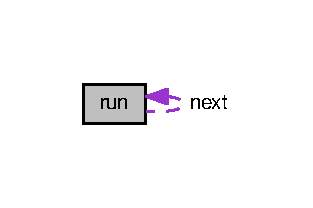
\includegraphics[width=150pt]{dc/dde/structrun__coll__graph}
\end{center}
\end{figure}
\subsection*{Public Attributes}
\begin{DoxyCompactItemize}
\item 
struct \hyperlink{structrun}{run} $\ast$ \hyperlink{structrun_a268099adb9e6c607cd814a421a1c8a18}{next}
\end{DoxyCompactItemize}


\subsection{Member Data Documentation}
\index{run@{run}!next@{next}}
\index{next@{next}!run@{run}}
\subsubsection[{\texorpdfstring{next}{next}}]{\setlength{\rightskip}{0pt plus 5cm}struct {\bf run}$\ast$ run\+::next}\hypertarget{structrun_a268099adb9e6c607cd814a421a1c8a18}{}\label{structrun_a268099adb9e6c607cd814a421a1c8a18}


The documentation for this struct was generated from the following file\+:\begin{DoxyCompactItemize}
\item 
\hyperlink{kalloc_8c}{kalloc.\+c}\end{DoxyCompactItemize}

\hypertarget{structsegdesc}{}\section{segdesc Struct Reference}
\label{structsegdesc}\index{segdesc@{segdesc}}


{\ttfamily \#include $<$mmu.\+h$>$}

\subsection*{Public Attributes}
\begin{DoxyCompactItemize}
\item 
\hyperlink{types_8h_a91ad9478d81a7aaf2593e8d9c3d06a14}{uint} \hyperlink{structsegdesc_a021002a4cf151893b5b8034b09cc7530}{lim\+\_\+15\+\_\+0}\+: 16
\item 
\hyperlink{types_8h_a91ad9478d81a7aaf2593e8d9c3d06a14}{uint} \hyperlink{structsegdesc_aaf95dd5b9105cf5729de49eb2542072a}{base\+\_\+15\+\_\+0}\+: 16
\item 
\hyperlink{types_8h_a91ad9478d81a7aaf2593e8d9c3d06a14}{uint} \hyperlink{structsegdesc_aa5cff1f1ddfac386e2268108c8f5b6c2}{base\+\_\+23\+\_\+16}\+: 8
\item 
\hyperlink{types_8h_a91ad9478d81a7aaf2593e8d9c3d06a14}{uint} \hyperlink{structsegdesc_acb54ea5ee6d09cfcc8b4dd3e96e4ce5b}{type}\+: 4
\item 
\hyperlink{types_8h_a91ad9478d81a7aaf2593e8d9c3d06a14}{uint} \hyperlink{structsegdesc_aacc67bb0857f0c77c1f8a5c9b8a1ac09}{s}\+: 1
\item 
\hyperlink{types_8h_a91ad9478d81a7aaf2593e8d9c3d06a14}{uint} \hyperlink{structsegdesc_ab22349cefd6990e4a9a1d93e42ee0c03}{dpl}\+: 2
\item 
\hyperlink{types_8h_a91ad9478d81a7aaf2593e8d9c3d06a14}{uint} \hyperlink{structsegdesc_a322a34a84a3815d35ebb3aa50c5a55e2}{p}\+: 1
\item 
\hyperlink{types_8h_a91ad9478d81a7aaf2593e8d9c3d06a14}{uint} \hyperlink{structsegdesc_abbc27a39a2ad6e59faa2eca33d7dfa0c}{lim\+\_\+19\+\_\+16}\+: 4
\item 
\hyperlink{types_8h_a91ad9478d81a7aaf2593e8d9c3d06a14}{uint} \hyperlink{structsegdesc_a6623d25de54a0a87d7a43ea4dfe7783f}{avl}\+: 1
\item 
\hyperlink{types_8h_a91ad9478d81a7aaf2593e8d9c3d06a14}{uint} \hyperlink{structsegdesc_a5798904f15e8fb63d2dd37e8a2818f0a}{rsv1}\+: 1
\item 
\hyperlink{types_8h_a91ad9478d81a7aaf2593e8d9c3d06a14}{uint} \hyperlink{structsegdesc_a08edbd480d21bfd147e304b6f5a3788f}{db}\+: 1
\item 
\hyperlink{types_8h_a91ad9478d81a7aaf2593e8d9c3d06a14}{uint} \hyperlink{structsegdesc_a6af7593606fa1a1ff003b4a78facc8e0}{g}\+: 1
\item 
\hyperlink{types_8h_a91ad9478d81a7aaf2593e8d9c3d06a14}{uint} \hyperlink{structsegdesc_a164a6a2e75fc62e61daef3ddab7f3169}{base\+\_\+31\+\_\+24}\+: 8
\end{DoxyCompactItemize}


\subsection{Member Data Documentation}
\index{segdesc@{segdesc}!avl@{avl}}
\index{avl@{avl}!segdesc@{segdesc}}
\subsubsection[{\texorpdfstring{avl}{avl}}]{\setlength{\rightskip}{0pt plus 5cm}{\bf uint} segdesc\+::avl}\hypertarget{structsegdesc_a6623d25de54a0a87d7a43ea4dfe7783f}{}\label{structsegdesc_a6623d25de54a0a87d7a43ea4dfe7783f}
\index{segdesc@{segdesc}!base\+\_\+15\+\_\+0@{base\+\_\+15\+\_\+0}}
\index{base\+\_\+15\+\_\+0@{base\+\_\+15\+\_\+0}!segdesc@{segdesc}}
\subsubsection[{\texorpdfstring{base\+\_\+15\+\_\+0}{base_15_0}}]{\setlength{\rightskip}{0pt plus 5cm}{\bf uint} segdesc\+::base\+\_\+15\+\_\+0}\hypertarget{structsegdesc_aaf95dd5b9105cf5729de49eb2542072a}{}\label{structsegdesc_aaf95dd5b9105cf5729de49eb2542072a}
\index{segdesc@{segdesc}!base\+\_\+23\+\_\+16@{base\+\_\+23\+\_\+16}}
\index{base\+\_\+23\+\_\+16@{base\+\_\+23\+\_\+16}!segdesc@{segdesc}}
\subsubsection[{\texorpdfstring{base\+\_\+23\+\_\+16}{base_23_16}}]{\setlength{\rightskip}{0pt plus 5cm}{\bf uint} segdesc\+::base\+\_\+23\+\_\+16}\hypertarget{structsegdesc_aa5cff1f1ddfac386e2268108c8f5b6c2}{}\label{structsegdesc_aa5cff1f1ddfac386e2268108c8f5b6c2}
\index{segdesc@{segdesc}!base\+\_\+31\+\_\+24@{base\+\_\+31\+\_\+24}}
\index{base\+\_\+31\+\_\+24@{base\+\_\+31\+\_\+24}!segdesc@{segdesc}}
\subsubsection[{\texorpdfstring{base\+\_\+31\+\_\+24}{base_31_24}}]{\setlength{\rightskip}{0pt plus 5cm}{\bf uint} segdesc\+::base\+\_\+31\+\_\+24}\hypertarget{structsegdesc_a164a6a2e75fc62e61daef3ddab7f3169}{}\label{structsegdesc_a164a6a2e75fc62e61daef3ddab7f3169}
\index{segdesc@{segdesc}!db@{db}}
\index{db@{db}!segdesc@{segdesc}}
\subsubsection[{\texorpdfstring{db}{db}}]{\setlength{\rightskip}{0pt plus 5cm}{\bf uint} segdesc\+::db}\hypertarget{structsegdesc_a08edbd480d21bfd147e304b6f5a3788f}{}\label{structsegdesc_a08edbd480d21bfd147e304b6f5a3788f}
\index{segdesc@{segdesc}!dpl@{dpl}}
\index{dpl@{dpl}!segdesc@{segdesc}}
\subsubsection[{\texorpdfstring{dpl}{dpl}}]{\setlength{\rightskip}{0pt plus 5cm}{\bf uint} segdesc\+::dpl}\hypertarget{structsegdesc_ab22349cefd6990e4a9a1d93e42ee0c03}{}\label{structsegdesc_ab22349cefd6990e4a9a1d93e42ee0c03}
\index{segdesc@{segdesc}!g@{g}}
\index{g@{g}!segdesc@{segdesc}}
\subsubsection[{\texorpdfstring{g}{g}}]{\setlength{\rightskip}{0pt plus 5cm}{\bf uint} segdesc\+::g}\hypertarget{structsegdesc_a6af7593606fa1a1ff003b4a78facc8e0}{}\label{structsegdesc_a6af7593606fa1a1ff003b4a78facc8e0}
\index{segdesc@{segdesc}!lim\+\_\+15\+\_\+0@{lim\+\_\+15\+\_\+0}}
\index{lim\+\_\+15\+\_\+0@{lim\+\_\+15\+\_\+0}!segdesc@{segdesc}}
\subsubsection[{\texorpdfstring{lim\+\_\+15\+\_\+0}{lim_15_0}}]{\setlength{\rightskip}{0pt plus 5cm}{\bf uint} segdesc\+::lim\+\_\+15\+\_\+0}\hypertarget{structsegdesc_a021002a4cf151893b5b8034b09cc7530}{}\label{structsegdesc_a021002a4cf151893b5b8034b09cc7530}
\index{segdesc@{segdesc}!lim\+\_\+19\+\_\+16@{lim\+\_\+19\+\_\+16}}
\index{lim\+\_\+19\+\_\+16@{lim\+\_\+19\+\_\+16}!segdesc@{segdesc}}
\subsubsection[{\texorpdfstring{lim\+\_\+19\+\_\+16}{lim_19_16}}]{\setlength{\rightskip}{0pt plus 5cm}{\bf uint} segdesc\+::lim\+\_\+19\+\_\+16}\hypertarget{structsegdesc_abbc27a39a2ad6e59faa2eca33d7dfa0c}{}\label{structsegdesc_abbc27a39a2ad6e59faa2eca33d7dfa0c}
\index{segdesc@{segdesc}!p@{p}}
\index{p@{p}!segdesc@{segdesc}}
\subsubsection[{\texorpdfstring{p}{p}}]{\setlength{\rightskip}{0pt plus 5cm}{\bf uint} segdesc\+::p}\hypertarget{structsegdesc_a322a34a84a3815d35ebb3aa50c5a55e2}{}\label{structsegdesc_a322a34a84a3815d35ebb3aa50c5a55e2}
\index{segdesc@{segdesc}!rsv1@{rsv1}}
\index{rsv1@{rsv1}!segdesc@{segdesc}}
\subsubsection[{\texorpdfstring{rsv1}{rsv1}}]{\setlength{\rightskip}{0pt plus 5cm}{\bf uint} segdesc\+::rsv1}\hypertarget{structsegdesc_a5798904f15e8fb63d2dd37e8a2818f0a}{}\label{structsegdesc_a5798904f15e8fb63d2dd37e8a2818f0a}
\index{segdesc@{segdesc}!s@{s}}
\index{s@{s}!segdesc@{segdesc}}
\subsubsection[{\texorpdfstring{s}{s}}]{\setlength{\rightskip}{0pt plus 5cm}{\bf uint} segdesc\+::s}\hypertarget{structsegdesc_aacc67bb0857f0c77c1f8a5c9b8a1ac09}{}\label{structsegdesc_aacc67bb0857f0c77c1f8a5c9b8a1ac09}
\index{segdesc@{segdesc}!type@{type}}
\index{type@{type}!segdesc@{segdesc}}
\subsubsection[{\texorpdfstring{type}{type}}]{\setlength{\rightskip}{0pt plus 5cm}{\bf uint} segdesc\+::type}\hypertarget{structsegdesc_acb54ea5ee6d09cfcc8b4dd3e96e4ce5b}{}\label{structsegdesc_acb54ea5ee6d09cfcc8b4dd3e96e4ce5b}


The documentation for this struct was generated from the following file\+:\begin{DoxyCompactItemize}
\item 
\hyperlink{mmu_8h}{mmu.\+h}\end{DoxyCompactItemize}

\hypertarget{structsleeplock}{}\section{sleeplock Struct Reference}
\label{structsleeplock}\index{sleeplock@{sleeplock}}


{\ttfamily \#include $<$sleeplock.\+h$>$}



Collaboration diagram for sleeplock\+:\nopagebreak
\begin{figure}[H]
\begin{center}
\leavevmode
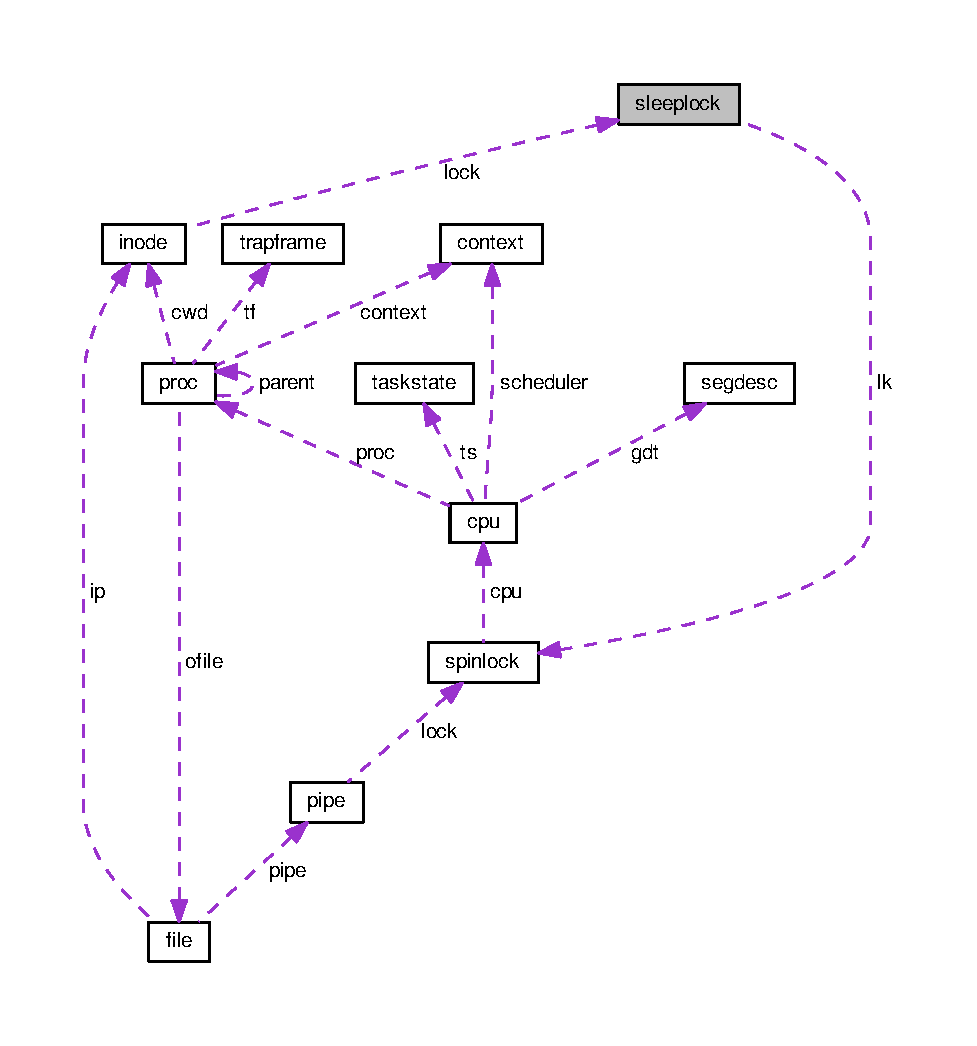
\includegraphics[width=350pt]{d9/d0a/structsleeplock__coll__graph}
\end{center}
\end{figure}
\subsection*{Public Attributes}
\begin{DoxyCompactItemize}
\item 
\hyperlink{types_8h_a91ad9478d81a7aaf2593e8d9c3d06a14}{uint} \hyperlink{structsleeplock_ac5cfe608994a41b24cb1c0fd722910c3}{locked}
\item 
struct \hyperlink{structspinlock}{spinlock} \hyperlink{structsleeplock_a077241ea0e720d228d853208444c4c9d}{lk}
\item 
char $\ast$ \hyperlink{structsleeplock_a40f1db61da688063cd5ac4f72d839590}{name}
\item 
int \hyperlink{structsleeplock_a99a4c6a784956ab1c391a12af475a55e}{pid}
\end{DoxyCompactItemize}


\subsection{Member Data Documentation}
\index{sleeplock@{sleeplock}!lk@{lk}}
\index{lk@{lk}!sleeplock@{sleeplock}}
\subsubsection[{\texorpdfstring{lk}{lk}}]{\setlength{\rightskip}{0pt plus 5cm}struct {\bf spinlock} sleeplock\+::lk}\hypertarget{structsleeplock_a077241ea0e720d228d853208444c4c9d}{}\label{structsleeplock_a077241ea0e720d228d853208444c4c9d}
\index{sleeplock@{sleeplock}!locked@{locked}}
\index{locked@{locked}!sleeplock@{sleeplock}}
\subsubsection[{\texorpdfstring{locked}{locked}}]{\setlength{\rightskip}{0pt plus 5cm}{\bf uint} sleeplock\+::locked}\hypertarget{structsleeplock_ac5cfe608994a41b24cb1c0fd722910c3}{}\label{structsleeplock_ac5cfe608994a41b24cb1c0fd722910c3}
\index{sleeplock@{sleeplock}!name@{name}}
\index{name@{name}!sleeplock@{sleeplock}}
\subsubsection[{\texorpdfstring{name}{name}}]{\setlength{\rightskip}{0pt plus 5cm}char$\ast$ sleeplock\+::name}\hypertarget{structsleeplock_a40f1db61da688063cd5ac4f72d839590}{}\label{structsleeplock_a40f1db61da688063cd5ac4f72d839590}
\index{sleeplock@{sleeplock}!pid@{pid}}
\index{pid@{pid}!sleeplock@{sleeplock}}
\subsubsection[{\texorpdfstring{pid}{pid}}]{\setlength{\rightskip}{0pt plus 5cm}int sleeplock\+::pid}\hypertarget{structsleeplock_a99a4c6a784956ab1c391a12af475a55e}{}\label{structsleeplock_a99a4c6a784956ab1c391a12af475a55e}


The documentation for this struct was generated from the following file\+:\begin{DoxyCompactItemize}
\item 
\hyperlink{sleeplock_8h}{sleeplock.\+h}\end{DoxyCompactItemize}

\hypertarget{structspinlock}{}\section{spinlock Struct Reference}
\label{structspinlock}\index{spinlock@{spinlock}}


{\ttfamily \#include $<$spinlock.\+h$>$}



Collaboration diagram for spinlock\+:\nopagebreak
\begin{figure}[H]
\begin{center}
\leavevmode
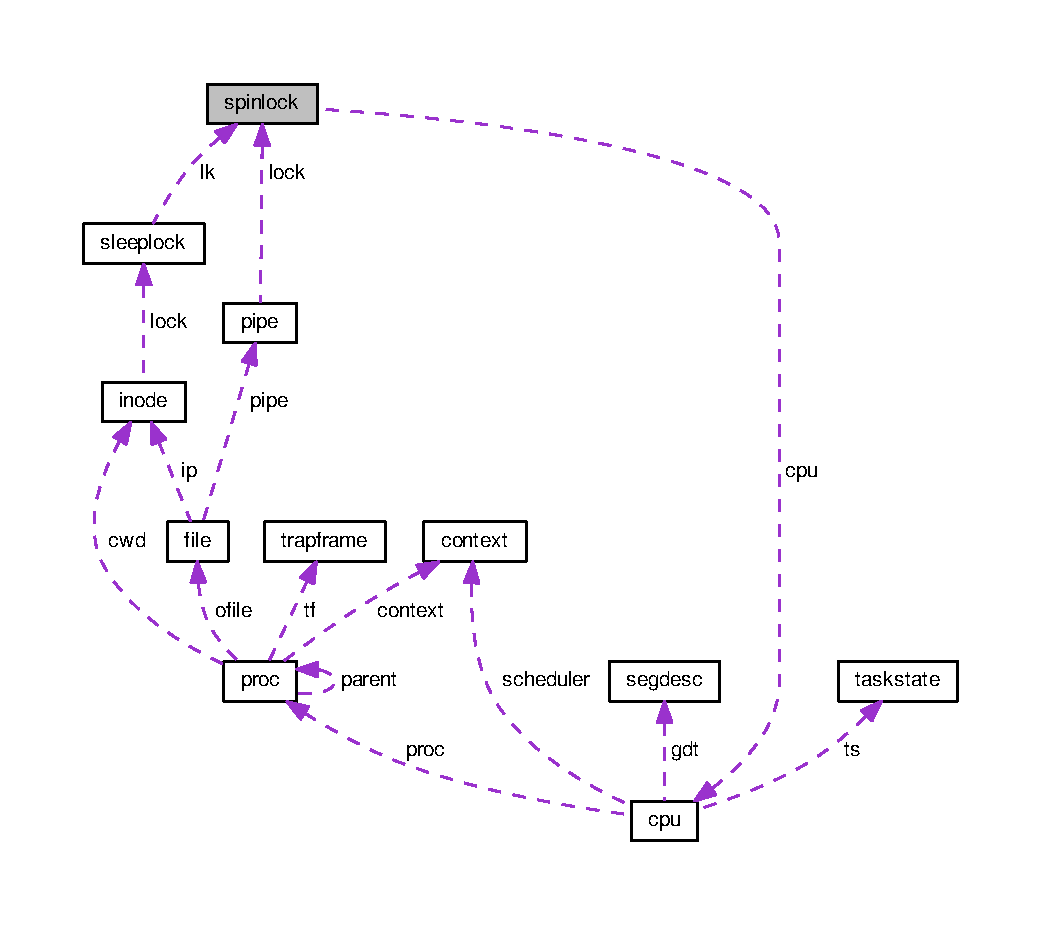
\includegraphics[width=350pt]{da/d23/structspinlock__coll__graph}
\end{center}
\end{figure}
\subsection*{Public Attributes}
\begin{DoxyCompactItemize}
\item 
\hyperlink{types_8h_a91ad9478d81a7aaf2593e8d9c3d06a14}{uint} \hyperlink{structspinlock_a48f3007579f644934d9aba91e5378c03}{locked}
\item 
char $\ast$ \hyperlink{structspinlock_afbec3274bf8ad9c421695a22f8d9d584}{name}
\item 
struct \hyperlink{structcpu}{cpu} $\ast$ \hyperlink{structspinlock_a290ae772c8ccb9e8c1580204c31a7f88}{cpu}
\item 
\hyperlink{types_8h_a91ad9478d81a7aaf2593e8d9c3d06a14}{uint} \hyperlink{structspinlock_ac9ef3f16f664094198af0b9063e23fe0}{pcs} \mbox{[}10\mbox{]}
\end{DoxyCompactItemize}


\subsection{Member Data Documentation}
\index{spinlock@{spinlock}!cpu@{cpu}}
\index{cpu@{cpu}!spinlock@{spinlock}}
\subsubsection[{\texorpdfstring{cpu}{cpu}}]{\setlength{\rightskip}{0pt plus 5cm}struct {\bf cpu}$\ast$ spinlock\+::cpu}\hypertarget{structspinlock_a290ae772c8ccb9e8c1580204c31a7f88}{}\label{structspinlock_a290ae772c8ccb9e8c1580204c31a7f88}
\index{spinlock@{spinlock}!locked@{locked}}
\index{locked@{locked}!spinlock@{spinlock}}
\subsubsection[{\texorpdfstring{locked}{locked}}]{\setlength{\rightskip}{0pt plus 5cm}{\bf uint} spinlock\+::locked}\hypertarget{structspinlock_a48f3007579f644934d9aba91e5378c03}{}\label{structspinlock_a48f3007579f644934d9aba91e5378c03}
\index{spinlock@{spinlock}!name@{name}}
\index{name@{name}!spinlock@{spinlock}}
\subsubsection[{\texorpdfstring{name}{name}}]{\setlength{\rightskip}{0pt plus 5cm}char$\ast$ spinlock\+::name}\hypertarget{structspinlock_afbec3274bf8ad9c421695a22f8d9d584}{}\label{structspinlock_afbec3274bf8ad9c421695a22f8d9d584}
\index{spinlock@{spinlock}!pcs@{pcs}}
\index{pcs@{pcs}!spinlock@{spinlock}}
\subsubsection[{\texorpdfstring{pcs}{pcs}}]{\setlength{\rightskip}{0pt plus 5cm}{\bf uint} spinlock\+::pcs\mbox{[}10\mbox{]}}\hypertarget{structspinlock_ac9ef3f16f664094198af0b9063e23fe0}{}\label{structspinlock_ac9ef3f16f664094198af0b9063e23fe0}


The documentation for this struct was generated from the following file\+:\begin{DoxyCompactItemize}
\item 
\hyperlink{spinlock_8h}{spinlock.\+h}\end{DoxyCompactItemize}

\hypertarget{structstat}{}\section{stat Struct Reference}
\label{structstat}\index{stat@{stat}}


{\ttfamily \#include $<$stat.\+h$>$}

\subsection*{Public Attributes}
\begin{DoxyCompactItemize}
\item 
short \hyperlink{structstat_a01f1b4cd7627d192a7875c9a188e0699}{type}
\item 
int \hyperlink{structstat_a14ef4f85e6fb86bf296360361d0f393b}{dev}
\item 
\hyperlink{types_8h_a91ad9478d81a7aaf2593e8d9c3d06a14}{uint} \hyperlink{structstat_abf15624517ed5d79d0fa2a5553a68e25}{ino}
\item 
short \hyperlink{structstat_a99ca3487fd2f4799337eb4281f8871e4}{nlink}
\item 
\hyperlink{types_8h_a91ad9478d81a7aaf2593e8d9c3d06a14}{uint} \hyperlink{structstat_a4ac15b64dd4d787c59a8a687d79adb35}{size}
\end{DoxyCompactItemize}


\subsection{Member Data Documentation}
\index{stat@{stat}!dev@{dev}}
\index{dev@{dev}!stat@{stat}}
\subsubsection[{\texorpdfstring{dev}{dev}}]{\setlength{\rightskip}{0pt plus 5cm}int stat\+::dev}\hypertarget{structstat_a14ef4f85e6fb86bf296360361d0f393b}{}\label{structstat_a14ef4f85e6fb86bf296360361d0f393b}
\index{stat@{stat}!ino@{ino}}
\index{ino@{ino}!stat@{stat}}
\subsubsection[{\texorpdfstring{ino}{ino}}]{\setlength{\rightskip}{0pt plus 5cm}{\bf uint} stat\+::ino}\hypertarget{structstat_abf15624517ed5d79d0fa2a5553a68e25}{}\label{structstat_abf15624517ed5d79d0fa2a5553a68e25}
\index{stat@{stat}!nlink@{nlink}}
\index{nlink@{nlink}!stat@{stat}}
\subsubsection[{\texorpdfstring{nlink}{nlink}}]{\setlength{\rightskip}{0pt plus 5cm}short stat\+::nlink}\hypertarget{structstat_a99ca3487fd2f4799337eb4281f8871e4}{}\label{structstat_a99ca3487fd2f4799337eb4281f8871e4}
\index{stat@{stat}!size@{size}}
\index{size@{size}!stat@{stat}}
\subsubsection[{\texorpdfstring{size}{size}}]{\setlength{\rightskip}{0pt plus 5cm}{\bf uint} stat\+::size}\hypertarget{structstat_a4ac15b64dd4d787c59a8a687d79adb35}{}\label{structstat_a4ac15b64dd4d787c59a8a687d79adb35}
\index{stat@{stat}!type@{type}}
\index{type@{type}!stat@{stat}}
\subsubsection[{\texorpdfstring{type}{type}}]{\setlength{\rightskip}{0pt plus 5cm}short stat\+::type}\hypertarget{structstat_a01f1b4cd7627d192a7875c9a188e0699}{}\label{structstat_a01f1b4cd7627d192a7875c9a188e0699}


The documentation for this struct was generated from the following file\+:\begin{DoxyCompactItemize}
\item 
\hyperlink{stat_8h}{stat.\+h}\end{DoxyCompactItemize}

\hypertarget{structsuperblock}{}\section{superblock Struct Reference}
\label{structsuperblock}\index{superblock@{superblock}}


{\ttfamily \#include $<$fs.\+h$>$}

\subsection*{Public Attributes}
\begin{DoxyCompactItemize}
\item 
\hyperlink{types_8h_a91ad9478d81a7aaf2593e8d9c3d06a14}{uint} \hyperlink{structsuperblock_a7c6e4d6da139ecee74eb7816d5d44fa6}{size}
\item 
\hyperlink{types_8h_a91ad9478d81a7aaf2593e8d9c3d06a14}{uint} \hyperlink{structsuperblock_a2a27a7cfb54689f0e1dcd1788d049218}{nblocks}
\item 
\hyperlink{types_8h_a91ad9478d81a7aaf2593e8d9c3d06a14}{uint} \hyperlink{structsuperblock_a355d2a1ebdc51f80820c23e69363cf42}{ninodes}
\item 
\hyperlink{types_8h_a91ad9478d81a7aaf2593e8d9c3d06a14}{uint} \hyperlink{structsuperblock_aea92ae872785fd4fb39b903d9157aac5}{nlog}
\item 
\hyperlink{types_8h_a91ad9478d81a7aaf2593e8d9c3d06a14}{uint} \hyperlink{structsuperblock_a460268b28aced19797e8d7b84aa60ebf}{logstart}
\item 
\hyperlink{types_8h_a91ad9478d81a7aaf2593e8d9c3d06a14}{uint} \hyperlink{structsuperblock_adde361528f3905445974301b424611c1}{inodestart}
\item 
\hyperlink{types_8h_a91ad9478d81a7aaf2593e8d9c3d06a14}{uint} \hyperlink{structsuperblock_a3c815dda5be6bda609389e76434171cc}{bmapstart}
\end{DoxyCompactItemize}


\subsection{Member Data Documentation}
\index{superblock@{superblock}!bmapstart@{bmapstart}}
\index{bmapstart@{bmapstart}!superblock@{superblock}}
\subsubsection[{\texorpdfstring{bmapstart}{bmapstart}}]{\setlength{\rightskip}{0pt plus 5cm}{\bf uint} superblock\+::bmapstart}\hypertarget{structsuperblock_a3c815dda5be6bda609389e76434171cc}{}\label{structsuperblock_a3c815dda5be6bda609389e76434171cc}
\index{superblock@{superblock}!inodestart@{inodestart}}
\index{inodestart@{inodestart}!superblock@{superblock}}
\subsubsection[{\texorpdfstring{inodestart}{inodestart}}]{\setlength{\rightskip}{0pt plus 5cm}{\bf uint} superblock\+::inodestart}\hypertarget{structsuperblock_adde361528f3905445974301b424611c1}{}\label{structsuperblock_adde361528f3905445974301b424611c1}
\index{superblock@{superblock}!logstart@{logstart}}
\index{logstart@{logstart}!superblock@{superblock}}
\subsubsection[{\texorpdfstring{logstart}{logstart}}]{\setlength{\rightskip}{0pt plus 5cm}{\bf uint} superblock\+::logstart}\hypertarget{structsuperblock_a460268b28aced19797e8d7b84aa60ebf}{}\label{structsuperblock_a460268b28aced19797e8d7b84aa60ebf}
\index{superblock@{superblock}!nblocks@{nblocks}}
\index{nblocks@{nblocks}!superblock@{superblock}}
\subsubsection[{\texorpdfstring{nblocks}{nblocks}}]{\setlength{\rightskip}{0pt plus 5cm}{\bf uint} superblock\+::nblocks}\hypertarget{structsuperblock_a2a27a7cfb54689f0e1dcd1788d049218}{}\label{structsuperblock_a2a27a7cfb54689f0e1dcd1788d049218}
\index{superblock@{superblock}!ninodes@{ninodes}}
\index{ninodes@{ninodes}!superblock@{superblock}}
\subsubsection[{\texorpdfstring{ninodes}{ninodes}}]{\setlength{\rightskip}{0pt plus 5cm}{\bf uint} superblock\+::ninodes}\hypertarget{structsuperblock_a355d2a1ebdc51f80820c23e69363cf42}{}\label{structsuperblock_a355d2a1ebdc51f80820c23e69363cf42}
\index{superblock@{superblock}!nlog@{nlog}}
\index{nlog@{nlog}!superblock@{superblock}}
\subsubsection[{\texorpdfstring{nlog}{nlog}}]{\setlength{\rightskip}{0pt plus 5cm}{\bf uint} superblock\+::nlog}\hypertarget{structsuperblock_aea92ae872785fd4fb39b903d9157aac5}{}\label{structsuperblock_aea92ae872785fd4fb39b903d9157aac5}
\index{superblock@{superblock}!size@{size}}
\index{size@{size}!superblock@{superblock}}
\subsubsection[{\texorpdfstring{size}{size}}]{\setlength{\rightskip}{0pt plus 5cm}{\bf uint} superblock\+::size}\hypertarget{structsuperblock_a7c6e4d6da139ecee74eb7816d5d44fa6}{}\label{structsuperblock_a7c6e4d6da139ecee74eb7816d5d44fa6}


The documentation for this struct was generated from the following file\+:\begin{DoxyCompactItemize}
\item 
\hyperlink{fs_8h}{fs.\+h}\end{DoxyCompactItemize}

\hypertarget{structtaskstate}{}\section{taskstate Struct Reference}
\label{structtaskstate}\index{taskstate@{taskstate}}


{\ttfamily \#include $<$mmu.\+h$>$}

\subsection*{Public Attributes}
\begin{DoxyCompactItemize}
\item 
\hyperlink{types_8h_a91ad9478d81a7aaf2593e8d9c3d06a14}{uint} \hyperlink{structtaskstate_a31a48a737b004273004ba8473ab6b0ed}{link}
\item 
\hyperlink{types_8h_a91ad9478d81a7aaf2593e8d9c3d06a14}{uint} \hyperlink{structtaskstate_a41b3e1d46a5068485eb6714974a979d6}{esp0}
\item 
\hyperlink{types_8h_ab95f123a6c9bcfee6a343170ef8c5f69}{ushort} \hyperlink{structtaskstate_a574e97ea3fd87f314da88afec3c6f574}{ss0}
\item 
\hyperlink{types_8h_ab95f123a6c9bcfee6a343170ef8c5f69}{ushort} \hyperlink{structtaskstate_a6b87ceb039ec11ccd265818673c53df5}{padding1}
\item 
\hyperlink{types_8h_a91ad9478d81a7aaf2593e8d9c3d06a14}{uint} $\ast$ \hyperlink{structtaskstate_a7ec69acf5f95163bd1ca2548fb0c541a}{esp1}
\item 
\hyperlink{types_8h_ab95f123a6c9bcfee6a343170ef8c5f69}{ushort} \hyperlink{structtaskstate_ac70c36414956cfee04c733a5b530d8ef}{ss1}
\item 
\hyperlink{types_8h_ab95f123a6c9bcfee6a343170ef8c5f69}{ushort} \hyperlink{structtaskstate_ae1bd6ae664d5899c3e118c21a27ba065}{padding2}
\item 
\hyperlink{types_8h_a91ad9478d81a7aaf2593e8d9c3d06a14}{uint} $\ast$ \hyperlink{structtaskstate_af206a117571ede3752b043e4e8cc6016}{esp2}
\item 
\hyperlink{types_8h_ab95f123a6c9bcfee6a343170ef8c5f69}{ushort} \hyperlink{structtaskstate_a573d8f57ef11630e782d8b7c924f28ce}{ss2}
\item 
\hyperlink{types_8h_ab95f123a6c9bcfee6a343170ef8c5f69}{ushort} \hyperlink{structtaskstate_a7989f7ea66e6e2100ef68c9e6964c231}{padding3}
\item 
void $\ast$ \hyperlink{structtaskstate_ac891b558913b4528fd2c9351c99da201}{cr3}
\item 
\hyperlink{types_8h_a91ad9478d81a7aaf2593e8d9c3d06a14}{uint} $\ast$ \hyperlink{structtaskstate_ae2bd660dd957f328d583e9a193dd250e}{eip}
\item 
\hyperlink{types_8h_a91ad9478d81a7aaf2593e8d9c3d06a14}{uint} \hyperlink{structtaskstate_a03952bc66789a00063ed9081c84cf01e}{eflags}
\item 
\hyperlink{types_8h_a91ad9478d81a7aaf2593e8d9c3d06a14}{uint} \hyperlink{structtaskstate_a6242c9879e9f87d1bcf5dfb6f3da4774}{eax}
\item 
\hyperlink{types_8h_a91ad9478d81a7aaf2593e8d9c3d06a14}{uint} \hyperlink{structtaskstate_a71af7c05a336906ef36771132ff5e804}{ecx}
\item 
\hyperlink{types_8h_a91ad9478d81a7aaf2593e8d9c3d06a14}{uint} \hyperlink{structtaskstate_a093193d42fe11c7d51e81fb41bfc0a60}{edx}
\item 
\hyperlink{types_8h_a91ad9478d81a7aaf2593e8d9c3d06a14}{uint} \hyperlink{structtaskstate_a0ef705c1f37c5c541ec9b688352e7b74}{ebx}
\item 
\hyperlink{types_8h_a91ad9478d81a7aaf2593e8d9c3d06a14}{uint} $\ast$ \hyperlink{structtaskstate_a9ee7c7c8cfe57f98eb72a6b8dd5342fa}{esp}
\item 
\hyperlink{types_8h_a91ad9478d81a7aaf2593e8d9c3d06a14}{uint} $\ast$ \hyperlink{structtaskstate_af20357700cba78c6e3a77610dcd47fb7}{ebp}
\item 
\hyperlink{types_8h_a91ad9478d81a7aaf2593e8d9c3d06a14}{uint} \hyperlink{structtaskstate_ab188878c1c090558d8d83a71282cc486}{esi}
\item 
\hyperlink{types_8h_a91ad9478d81a7aaf2593e8d9c3d06a14}{uint} \hyperlink{structtaskstate_a32fc8c63c3843c7ea2a675158498a029}{edi}
\item 
\hyperlink{types_8h_ab95f123a6c9bcfee6a343170ef8c5f69}{ushort} \hyperlink{structtaskstate_afcc56f9f9cba058c518a021babe00d9a}{es}
\item 
\hyperlink{types_8h_ab95f123a6c9bcfee6a343170ef8c5f69}{ushort} \hyperlink{structtaskstate_a9905f5108c60aab4b6e5c2a1ce1ce356}{padding4}
\item 
\hyperlink{types_8h_ab95f123a6c9bcfee6a343170ef8c5f69}{ushort} \hyperlink{structtaskstate_aec68e08358623490628d50e0ff9448f4}{cs}
\item 
\hyperlink{types_8h_ab95f123a6c9bcfee6a343170ef8c5f69}{ushort} \hyperlink{structtaskstate_ad462c3b654306417c32c78f42b5a9e42}{padding5}
\item 
\hyperlink{types_8h_ab95f123a6c9bcfee6a343170ef8c5f69}{ushort} \hyperlink{structtaskstate_afdd8f3985ac7ae69fc67c19d65653f12}{ss}
\item 
\hyperlink{types_8h_ab95f123a6c9bcfee6a343170ef8c5f69}{ushort} \hyperlink{structtaskstate_a3885094380c4d991fa86d31fdf1b9683}{padding6}
\item 
\hyperlink{types_8h_ab95f123a6c9bcfee6a343170ef8c5f69}{ushort} \hyperlink{structtaskstate_af5f19782df3eb439445274e08d9120f1}{ds}
\item 
\hyperlink{types_8h_ab95f123a6c9bcfee6a343170ef8c5f69}{ushort} \hyperlink{structtaskstate_a4c634b4b3cd489ca37979561394bf518}{padding7}
\item 
\hyperlink{types_8h_ab95f123a6c9bcfee6a343170ef8c5f69}{ushort} \hyperlink{structtaskstate_a4ce0e6f25b9721d7e2660c8840a0f9e3}{fs}
\item 
\hyperlink{types_8h_ab95f123a6c9bcfee6a343170ef8c5f69}{ushort} \hyperlink{structtaskstate_ab3077e8c9fe9b50ff7caedeeac075472}{padding8}
\item 
\hyperlink{types_8h_ab95f123a6c9bcfee6a343170ef8c5f69}{ushort} \hyperlink{structtaskstate_a15529ac51461a168be78130042a740e7}{gs}
\item 
\hyperlink{types_8h_ab95f123a6c9bcfee6a343170ef8c5f69}{ushort} \hyperlink{structtaskstate_a58a780ba0664e4ff8741adbdaccbcdd5}{padding9}
\item 
\hyperlink{types_8h_ab95f123a6c9bcfee6a343170ef8c5f69}{ushort} \hyperlink{structtaskstate_a960e5d4a40dcafb35f32ec047c0ca147}{ldt}
\item 
\hyperlink{types_8h_ab95f123a6c9bcfee6a343170ef8c5f69}{ushort} \hyperlink{structtaskstate_a6f95dd6d0ae39afaaf5ee8671220b00b}{padding10}
\item 
\hyperlink{types_8h_ab95f123a6c9bcfee6a343170ef8c5f69}{ushort} \hyperlink{structtaskstate_ad9d64e6139f851a3f8d2275f2748fae5}{t}
\item 
\hyperlink{types_8h_ab95f123a6c9bcfee6a343170ef8c5f69}{ushort} \hyperlink{structtaskstate_a5ee57b190324239a5d88f7c02039901f}{iomb}
\end{DoxyCompactItemize}


\subsection{Member Data Documentation}
\index{taskstate@{taskstate}!cr3@{cr3}}
\index{cr3@{cr3}!taskstate@{taskstate}}
\subsubsection[{\texorpdfstring{cr3}{cr3}}]{\setlength{\rightskip}{0pt plus 5cm}void$\ast$ taskstate\+::cr3}\hypertarget{structtaskstate_ac891b558913b4528fd2c9351c99da201}{}\label{structtaskstate_ac891b558913b4528fd2c9351c99da201}
\index{taskstate@{taskstate}!cs@{cs}}
\index{cs@{cs}!taskstate@{taskstate}}
\subsubsection[{\texorpdfstring{cs}{cs}}]{\setlength{\rightskip}{0pt plus 5cm}{\bf ushort} taskstate\+::cs}\hypertarget{structtaskstate_aec68e08358623490628d50e0ff9448f4}{}\label{structtaskstate_aec68e08358623490628d50e0ff9448f4}
\index{taskstate@{taskstate}!ds@{ds}}
\index{ds@{ds}!taskstate@{taskstate}}
\subsubsection[{\texorpdfstring{ds}{ds}}]{\setlength{\rightskip}{0pt plus 5cm}{\bf ushort} taskstate\+::ds}\hypertarget{structtaskstate_af5f19782df3eb439445274e08d9120f1}{}\label{structtaskstate_af5f19782df3eb439445274e08d9120f1}
\index{taskstate@{taskstate}!eax@{eax}}
\index{eax@{eax}!taskstate@{taskstate}}
\subsubsection[{\texorpdfstring{eax}{eax}}]{\setlength{\rightskip}{0pt plus 5cm}{\bf uint} taskstate\+::eax}\hypertarget{structtaskstate_a6242c9879e9f87d1bcf5dfb6f3da4774}{}\label{structtaskstate_a6242c9879e9f87d1bcf5dfb6f3da4774}
\index{taskstate@{taskstate}!ebp@{ebp}}
\index{ebp@{ebp}!taskstate@{taskstate}}
\subsubsection[{\texorpdfstring{ebp}{ebp}}]{\setlength{\rightskip}{0pt plus 5cm}{\bf uint}$\ast$ taskstate\+::ebp}\hypertarget{structtaskstate_af20357700cba78c6e3a77610dcd47fb7}{}\label{structtaskstate_af20357700cba78c6e3a77610dcd47fb7}
\index{taskstate@{taskstate}!ebx@{ebx}}
\index{ebx@{ebx}!taskstate@{taskstate}}
\subsubsection[{\texorpdfstring{ebx}{ebx}}]{\setlength{\rightskip}{0pt plus 5cm}{\bf uint} taskstate\+::ebx}\hypertarget{structtaskstate_a0ef705c1f37c5c541ec9b688352e7b74}{}\label{structtaskstate_a0ef705c1f37c5c541ec9b688352e7b74}
\index{taskstate@{taskstate}!ecx@{ecx}}
\index{ecx@{ecx}!taskstate@{taskstate}}
\subsubsection[{\texorpdfstring{ecx}{ecx}}]{\setlength{\rightskip}{0pt plus 5cm}{\bf uint} taskstate\+::ecx}\hypertarget{structtaskstate_a71af7c05a336906ef36771132ff5e804}{}\label{structtaskstate_a71af7c05a336906ef36771132ff5e804}
\index{taskstate@{taskstate}!edi@{edi}}
\index{edi@{edi}!taskstate@{taskstate}}
\subsubsection[{\texorpdfstring{edi}{edi}}]{\setlength{\rightskip}{0pt plus 5cm}{\bf uint} taskstate\+::edi}\hypertarget{structtaskstate_a32fc8c63c3843c7ea2a675158498a029}{}\label{structtaskstate_a32fc8c63c3843c7ea2a675158498a029}
\index{taskstate@{taskstate}!edx@{edx}}
\index{edx@{edx}!taskstate@{taskstate}}
\subsubsection[{\texorpdfstring{edx}{edx}}]{\setlength{\rightskip}{0pt plus 5cm}{\bf uint} taskstate\+::edx}\hypertarget{structtaskstate_a093193d42fe11c7d51e81fb41bfc0a60}{}\label{structtaskstate_a093193d42fe11c7d51e81fb41bfc0a60}
\index{taskstate@{taskstate}!eflags@{eflags}}
\index{eflags@{eflags}!taskstate@{taskstate}}
\subsubsection[{\texorpdfstring{eflags}{eflags}}]{\setlength{\rightskip}{0pt plus 5cm}{\bf uint} taskstate\+::eflags}\hypertarget{structtaskstate_a03952bc66789a00063ed9081c84cf01e}{}\label{structtaskstate_a03952bc66789a00063ed9081c84cf01e}
\index{taskstate@{taskstate}!eip@{eip}}
\index{eip@{eip}!taskstate@{taskstate}}
\subsubsection[{\texorpdfstring{eip}{eip}}]{\setlength{\rightskip}{0pt plus 5cm}{\bf uint}$\ast$ taskstate\+::eip}\hypertarget{structtaskstate_ae2bd660dd957f328d583e9a193dd250e}{}\label{structtaskstate_ae2bd660dd957f328d583e9a193dd250e}
\index{taskstate@{taskstate}!es@{es}}
\index{es@{es}!taskstate@{taskstate}}
\subsubsection[{\texorpdfstring{es}{es}}]{\setlength{\rightskip}{0pt plus 5cm}{\bf ushort} taskstate\+::es}\hypertarget{structtaskstate_afcc56f9f9cba058c518a021babe00d9a}{}\label{structtaskstate_afcc56f9f9cba058c518a021babe00d9a}
\index{taskstate@{taskstate}!esi@{esi}}
\index{esi@{esi}!taskstate@{taskstate}}
\subsubsection[{\texorpdfstring{esi}{esi}}]{\setlength{\rightskip}{0pt plus 5cm}{\bf uint} taskstate\+::esi}\hypertarget{structtaskstate_ab188878c1c090558d8d83a71282cc486}{}\label{structtaskstate_ab188878c1c090558d8d83a71282cc486}
\index{taskstate@{taskstate}!esp@{esp}}
\index{esp@{esp}!taskstate@{taskstate}}
\subsubsection[{\texorpdfstring{esp}{esp}}]{\setlength{\rightskip}{0pt plus 5cm}{\bf uint}$\ast$ taskstate\+::esp}\hypertarget{structtaskstate_a9ee7c7c8cfe57f98eb72a6b8dd5342fa}{}\label{structtaskstate_a9ee7c7c8cfe57f98eb72a6b8dd5342fa}
\index{taskstate@{taskstate}!esp0@{esp0}}
\index{esp0@{esp0}!taskstate@{taskstate}}
\subsubsection[{\texorpdfstring{esp0}{esp0}}]{\setlength{\rightskip}{0pt plus 5cm}{\bf uint} taskstate\+::esp0}\hypertarget{structtaskstate_a41b3e1d46a5068485eb6714974a979d6}{}\label{structtaskstate_a41b3e1d46a5068485eb6714974a979d6}
\index{taskstate@{taskstate}!esp1@{esp1}}
\index{esp1@{esp1}!taskstate@{taskstate}}
\subsubsection[{\texorpdfstring{esp1}{esp1}}]{\setlength{\rightskip}{0pt plus 5cm}{\bf uint}$\ast$ taskstate\+::esp1}\hypertarget{structtaskstate_a7ec69acf5f95163bd1ca2548fb0c541a}{}\label{structtaskstate_a7ec69acf5f95163bd1ca2548fb0c541a}
\index{taskstate@{taskstate}!esp2@{esp2}}
\index{esp2@{esp2}!taskstate@{taskstate}}
\subsubsection[{\texorpdfstring{esp2}{esp2}}]{\setlength{\rightskip}{0pt plus 5cm}{\bf uint}$\ast$ taskstate\+::esp2}\hypertarget{structtaskstate_af206a117571ede3752b043e4e8cc6016}{}\label{structtaskstate_af206a117571ede3752b043e4e8cc6016}
\index{taskstate@{taskstate}!fs@{fs}}
\index{fs@{fs}!taskstate@{taskstate}}
\subsubsection[{\texorpdfstring{fs}{fs}}]{\setlength{\rightskip}{0pt plus 5cm}{\bf ushort} taskstate\+::fs}\hypertarget{structtaskstate_a4ce0e6f25b9721d7e2660c8840a0f9e3}{}\label{structtaskstate_a4ce0e6f25b9721d7e2660c8840a0f9e3}
\index{taskstate@{taskstate}!gs@{gs}}
\index{gs@{gs}!taskstate@{taskstate}}
\subsubsection[{\texorpdfstring{gs}{gs}}]{\setlength{\rightskip}{0pt plus 5cm}{\bf ushort} taskstate\+::gs}\hypertarget{structtaskstate_a15529ac51461a168be78130042a740e7}{}\label{structtaskstate_a15529ac51461a168be78130042a740e7}
\index{taskstate@{taskstate}!iomb@{iomb}}
\index{iomb@{iomb}!taskstate@{taskstate}}
\subsubsection[{\texorpdfstring{iomb}{iomb}}]{\setlength{\rightskip}{0pt plus 5cm}{\bf ushort} taskstate\+::iomb}\hypertarget{structtaskstate_a5ee57b190324239a5d88f7c02039901f}{}\label{structtaskstate_a5ee57b190324239a5d88f7c02039901f}
\index{taskstate@{taskstate}!ldt@{ldt}}
\index{ldt@{ldt}!taskstate@{taskstate}}
\subsubsection[{\texorpdfstring{ldt}{ldt}}]{\setlength{\rightskip}{0pt plus 5cm}{\bf ushort} taskstate\+::ldt}\hypertarget{structtaskstate_a960e5d4a40dcafb35f32ec047c0ca147}{}\label{structtaskstate_a960e5d4a40dcafb35f32ec047c0ca147}
\index{taskstate@{taskstate}!link@{link}}
\index{link@{link}!taskstate@{taskstate}}
\subsubsection[{\texorpdfstring{link}{link}}]{\setlength{\rightskip}{0pt plus 5cm}{\bf uint} taskstate\+::link}\hypertarget{structtaskstate_a31a48a737b004273004ba8473ab6b0ed}{}\label{structtaskstate_a31a48a737b004273004ba8473ab6b0ed}
\index{taskstate@{taskstate}!padding1@{padding1}}
\index{padding1@{padding1}!taskstate@{taskstate}}
\subsubsection[{\texorpdfstring{padding1}{padding1}}]{\setlength{\rightskip}{0pt plus 5cm}{\bf ushort} taskstate\+::padding1}\hypertarget{structtaskstate_a6b87ceb039ec11ccd265818673c53df5}{}\label{structtaskstate_a6b87ceb039ec11ccd265818673c53df5}
\index{taskstate@{taskstate}!padding10@{padding10}}
\index{padding10@{padding10}!taskstate@{taskstate}}
\subsubsection[{\texorpdfstring{padding10}{padding10}}]{\setlength{\rightskip}{0pt plus 5cm}{\bf ushort} taskstate\+::padding10}\hypertarget{structtaskstate_a6f95dd6d0ae39afaaf5ee8671220b00b}{}\label{structtaskstate_a6f95dd6d0ae39afaaf5ee8671220b00b}
\index{taskstate@{taskstate}!padding2@{padding2}}
\index{padding2@{padding2}!taskstate@{taskstate}}
\subsubsection[{\texorpdfstring{padding2}{padding2}}]{\setlength{\rightskip}{0pt plus 5cm}{\bf ushort} taskstate\+::padding2}\hypertarget{structtaskstate_ae1bd6ae664d5899c3e118c21a27ba065}{}\label{structtaskstate_ae1bd6ae664d5899c3e118c21a27ba065}
\index{taskstate@{taskstate}!padding3@{padding3}}
\index{padding3@{padding3}!taskstate@{taskstate}}
\subsubsection[{\texorpdfstring{padding3}{padding3}}]{\setlength{\rightskip}{0pt plus 5cm}{\bf ushort} taskstate\+::padding3}\hypertarget{structtaskstate_a7989f7ea66e6e2100ef68c9e6964c231}{}\label{structtaskstate_a7989f7ea66e6e2100ef68c9e6964c231}
\index{taskstate@{taskstate}!padding4@{padding4}}
\index{padding4@{padding4}!taskstate@{taskstate}}
\subsubsection[{\texorpdfstring{padding4}{padding4}}]{\setlength{\rightskip}{0pt plus 5cm}{\bf ushort} taskstate\+::padding4}\hypertarget{structtaskstate_a9905f5108c60aab4b6e5c2a1ce1ce356}{}\label{structtaskstate_a9905f5108c60aab4b6e5c2a1ce1ce356}
\index{taskstate@{taskstate}!padding5@{padding5}}
\index{padding5@{padding5}!taskstate@{taskstate}}
\subsubsection[{\texorpdfstring{padding5}{padding5}}]{\setlength{\rightskip}{0pt plus 5cm}{\bf ushort} taskstate\+::padding5}\hypertarget{structtaskstate_ad462c3b654306417c32c78f42b5a9e42}{}\label{structtaskstate_ad462c3b654306417c32c78f42b5a9e42}
\index{taskstate@{taskstate}!padding6@{padding6}}
\index{padding6@{padding6}!taskstate@{taskstate}}
\subsubsection[{\texorpdfstring{padding6}{padding6}}]{\setlength{\rightskip}{0pt plus 5cm}{\bf ushort} taskstate\+::padding6}\hypertarget{structtaskstate_a3885094380c4d991fa86d31fdf1b9683}{}\label{structtaskstate_a3885094380c4d991fa86d31fdf1b9683}
\index{taskstate@{taskstate}!padding7@{padding7}}
\index{padding7@{padding7}!taskstate@{taskstate}}
\subsubsection[{\texorpdfstring{padding7}{padding7}}]{\setlength{\rightskip}{0pt plus 5cm}{\bf ushort} taskstate\+::padding7}\hypertarget{structtaskstate_a4c634b4b3cd489ca37979561394bf518}{}\label{structtaskstate_a4c634b4b3cd489ca37979561394bf518}
\index{taskstate@{taskstate}!padding8@{padding8}}
\index{padding8@{padding8}!taskstate@{taskstate}}
\subsubsection[{\texorpdfstring{padding8}{padding8}}]{\setlength{\rightskip}{0pt plus 5cm}{\bf ushort} taskstate\+::padding8}\hypertarget{structtaskstate_ab3077e8c9fe9b50ff7caedeeac075472}{}\label{structtaskstate_ab3077e8c9fe9b50ff7caedeeac075472}
\index{taskstate@{taskstate}!padding9@{padding9}}
\index{padding9@{padding9}!taskstate@{taskstate}}
\subsubsection[{\texorpdfstring{padding9}{padding9}}]{\setlength{\rightskip}{0pt plus 5cm}{\bf ushort} taskstate\+::padding9}\hypertarget{structtaskstate_a58a780ba0664e4ff8741adbdaccbcdd5}{}\label{structtaskstate_a58a780ba0664e4ff8741adbdaccbcdd5}
\index{taskstate@{taskstate}!ss@{ss}}
\index{ss@{ss}!taskstate@{taskstate}}
\subsubsection[{\texorpdfstring{ss}{ss}}]{\setlength{\rightskip}{0pt plus 5cm}{\bf ushort} taskstate\+::ss}\hypertarget{structtaskstate_afdd8f3985ac7ae69fc67c19d65653f12}{}\label{structtaskstate_afdd8f3985ac7ae69fc67c19d65653f12}
\index{taskstate@{taskstate}!ss0@{ss0}}
\index{ss0@{ss0}!taskstate@{taskstate}}
\subsubsection[{\texorpdfstring{ss0}{ss0}}]{\setlength{\rightskip}{0pt plus 5cm}{\bf ushort} taskstate\+::ss0}\hypertarget{structtaskstate_a574e97ea3fd87f314da88afec3c6f574}{}\label{structtaskstate_a574e97ea3fd87f314da88afec3c6f574}
\index{taskstate@{taskstate}!ss1@{ss1}}
\index{ss1@{ss1}!taskstate@{taskstate}}
\subsubsection[{\texorpdfstring{ss1}{ss1}}]{\setlength{\rightskip}{0pt plus 5cm}{\bf ushort} taskstate\+::ss1}\hypertarget{structtaskstate_ac70c36414956cfee04c733a5b530d8ef}{}\label{structtaskstate_ac70c36414956cfee04c733a5b530d8ef}
\index{taskstate@{taskstate}!ss2@{ss2}}
\index{ss2@{ss2}!taskstate@{taskstate}}
\subsubsection[{\texorpdfstring{ss2}{ss2}}]{\setlength{\rightskip}{0pt plus 5cm}{\bf ushort} taskstate\+::ss2}\hypertarget{structtaskstate_a573d8f57ef11630e782d8b7c924f28ce}{}\label{structtaskstate_a573d8f57ef11630e782d8b7c924f28ce}
\index{taskstate@{taskstate}!t@{t}}
\index{t@{t}!taskstate@{taskstate}}
\subsubsection[{\texorpdfstring{t}{t}}]{\setlength{\rightskip}{0pt plus 5cm}{\bf ushort} taskstate\+::t}\hypertarget{structtaskstate_ad9d64e6139f851a3f8d2275f2748fae5}{}\label{structtaskstate_ad9d64e6139f851a3f8d2275f2748fae5}


The documentation for this struct was generated from the following file\+:\begin{DoxyCompactItemize}
\item 
\hyperlink{mmu_8h}{mmu.\+h}\end{DoxyCompactItemize}

\hypertarget{structtrapframe}{}\section{trapframe Struct Reference}
\label{structtrapframe}\index{trapframe@{trapframe}}


{\ttfamily \#include $<$x86.\+h$>$}

\subsection*{Public Attributes}
\begin{DoxyCompactItemize}
\item 
\hyperlink{types_8h_a91ad9478d81a7aaf2593e8d9c3d06a14}{uint} \hyperlink{structtrapframe_ad20959553b558987a0d475b6367c87d0}{edi}
\item 
\hyperlink{types_8h_a91ad9478d81a7aaf2593e8d9c3d06a14}{uint} \hyperlink{structtrapframe_a11cbc20a968f2ce7a9b71590a709bb46}{esi}
\item 
\hyperlink{types_8h_a91ad9478d81a7aaf2593e8d9c3d06a14}{uint} \hyperlink{structtrapframe_a258f414f983f95f6799372d548fbd6d3}{ebp}
\item 
\hyperlink{types_8h_a91ad9478d81a7aaf2593e8d9c3d06a14}{uint} \hyperlink{structtrapframe_a8466e7bcbbbe2d19fbe7f4fe0daa29fb}{oesp}
\item 
\hyperlink{types_8h_a91ad9478d81a7aaf2593e8d9c3d06a14}{uint} \hyperlink{structtrapframe_a0f93026966ea52a69a94870fb394ba04}{ebx}
\item 
\hyperlink{types_8h_a91ad9478d81a7aaf2593e8d9c3d06a14}{uint} \hyperlink{structtrapframe_a62585fbda8434a03de564611b89c02ad}{edx}
\item 
\hyperlink{types_8h_a91ad9478d81a7aaf2593e8d9c3d06a14}{uint} \hyperlink{structtrapframe_ad42fe2bbc83c7fe778f0127ac038efa3}{ecx}
\item 
\hyperlink{types_8h_a91ad9478d81a7aaf2593e8d9c3d06a14}{uint} \hyperlink{structtrapframe_ab1dd3a10936b61129d7395c3a21bc2fe}{eax}
\item 
\hyperlink{types_8h_ab95f123a6c9bcfee6a343170ef8c5f69}{ushort} \hyperlink{structtrapframe_a3df62e3ed00405cbaaa4d72902c617da}{gs}
\item 
\hyperlink{types_8h_ab95f123a6c9bcfee6a343170ef8c5f69}{ushort} \hyperlink{structtrapframe_a84a5fbe43d7f11df983d97c80aabb454}{padding1}
\item 
\hyperlink{types_8h_ab95f123a6c9bcfee6a343170ef8c5f69}{ushort} \hyperlink{structtrapframe_a4791a272cca7213d324e59db2d9d0b71}{fs}
\item 
\hyperlink{types_8h_ab95f123a6c9bcfee6a343170ef8c5f69}{ushort} \hyperlink{structtrapframe_a63737765c58491a8604ef180a3864ad0}{padding2}
\item 
\hyperlink{types_8h_ab95f123a6c9bcfee6a343170ef8c5f69}{ushort} \hyperlink{structtrapframe_ab974b358098da0aaa5897c32827a038d}{es}
\item 
\hyperlink{types_8h_ab95f123a6c9bcfee6a343170ef8c5f69}{ushort} \hyperlink{structtrapframe_acd8a8fee013b35212fab787b645f8dd9}{padding3}
\item 
\hyperlink{types_8h_ab95f123a6c9bcfee6a343170ef8c5f69}{ushort} \hyperlink{structtrapframe_a421be1ec9ad2a55f1d1adeac9b0b89c3}{ds}
\item 
\hyperlink{types_8h_ab95f123a6c9bcfee6a343170ef8c5f69}{ushort} \hyperlink{structtrapframe_aef4bc72b31fb4a0cf6b32782b40a7e2f}{padding4}
\item 
\hyperlink{types_8h_a91ad9478d81a7aaf2593e8d9c3d06a14}{uint} \hyperlink{structtrapframe_abc7f81b0a6a91d13e9fefe171b0a7d12}{trapno}
\item 
\hyperlink{types_8h_a91ad9478d81a7aaf2593e8d9c3d06a14}{uint} \hyperlink{structtrapframe_acfb2346e6184b0d2438960b4f2a67e4f}{err}
\item 
\hyperlink{types_8h_a91ad9478d81a7aaf2593e8d9c3d06a14}{uint} \hyperlink{structtrapframe_a886a5973a537894e3a95435f38767d5c}{eip}
\item 
\hyperlink{types_8h_ab95f123a6c9bcfee6a343170ef8c5f69}{ushort} \hyperlink{structtrapframe_a61261f63223a73e25be79fcc8c625265}{cs}
\item 
\hyperlink{types_8h_ab95f123a6c9bcfee6a343170ef8c5f69}{ushort} \hyperlink{structtrapframe_a5715f786df145b0bf6faf3aa3304f05f}{padding5}
\item 
\hyperlink{types_8h_a91ad9478d81a7aaf2593e8d9c3d06a14}{uint} \hyperlink{structtrapframe_ae6b3005ad34416546603ab18dbb4a644}{eflags}
\item 
\hyperlink{types_8h_a91ad9478d81a7aaf2593e8d9c3d06a14}{uint} \hyperlink{structtrapframe_acd319e2dbd720d217c10f8fb620d73e2}{esp}
\item 
\hyperlink{types_8h_ab95f123a6c9bcfee6a343170ef8c5f69}{ushort} \hyperlink{structtrapframe_aa9c9b52b242d4f42fe4252e26b655bf6}{ss}
\item 
\hyperlink{types_8h_ab95f123a6c9bcfee6a343170ef8c5f69}{ushort} \hyperlink{structtrapframe_a1c079b271df9fdd3502bfe9e00888dfa}{padding6}
\end{DoxyCompactItemize}


\subsection{Member Data Documentation}
\index{trapframe@{trapframe}!cs@{cs}}
\index{cs@{cs}!trapframe@{trapframe}}
\subsubsection[{\texorpdfstring{cs}{cs}}]{\setlength{\rightskip}{0pt plus 5cm}{\bf ushort} trapframe\+::cs}\hypertarget{structtrapframe_a61261f63223a73e25be79fcc8c625265}{}\label{structtrapframe_a61261f63223a73e25be79fcc8c625265}
\index{trapframe@{trapframe}!ds@{ds}}
\index{ds@{ds}!trapframe@{trapframe}}
\subsubsection[{\texorpdfstring{ds}{ds}}]{\setlength{\rightskip}{0pt plus 5cm}{\bf ushort} trapframe\+::ds}\hypertarget{structtrapframe_a421be1ec9ad2a55f1d1adeac9b0b89c3}{}\label{structtrapframe_a421be1ec9ad2a55f1d1adeac9b0b89c3}
\index{trapframe@{trapframe}!eax@{eax}}
\index{eax@{eax}!trapframe@{trapframe}}
\subsubsection[{\texorpdfstring{eax}{eax}}]{\setlength{\rightskip}{0pt plus 5cm}{\bf uint} trapframe\+::eax}\hypertarget{structtrapframe_ab1dd3a10936b61129d7395c3a21bc2fe}{}\label{structtrapframe_ab1dd3a10936b61129d7395c3a21bc2fe}
\index{trapframe@{trapframe}!ebp@{ebp}}
\index{ebp@{ebp}!trapframe@{trapframe}}
\subsubsection[{\texorpdfstring{ebp}{ebp}}]{\setlength{\rightskip}{0pt plus 5cm}{\bf uint} trapframe\+::ebp}\hypertarget{structtrapframe_a258f414f983f95f6799372d548fbd6d3}{}\label{structtrapframe_a258f414f983f95f6799372d548fbd6d3}
\index{trapframe@{trapframe}!ebx@{ebx}}
\index{ebx@{ebx}!trapframe@{trapframe}}
\subsubsection[{\texorpdfstring{ebx}{ebx}}]{\setlength{\rightskip}{0pt plus 5cm}{\bf uint} trapframe\+::ebx}\hypertarget{structtrapframe_a0f93026966ea52a69a94870fb394ba04}{}\label{structtrapframe_a0f93026966ea52a69a94870fb394ba04}
\index{trapframe@{trapframe}!ecx@{ecx}}
\index{ecx@{ecx}!trapframe@{trapframe}}
\subsubsection[{\texorpdfstring{ecx}{ecx}}]{\setlength{\rightskip}{0pt plus 5cm}{\bf uint} trapframe\+::ecx}\hypertarget{structtrapframe_ad42fe2bbc83c7fe778f0127ac038efa3}{}\label{structtrapframe_ad42fe2bbc83c7fe778f0127ac038efa3}
\index{trapframe@{trapframe}!edi@{edi}}
\index{edi@{edi}!trapframe@{trapframe}}
\subsubsection[{\texorpdfstring{edi}{edi}}]{\setlength{\rightskip}{0pt plus 5cm}{\bf uint} trapframe\+::edi}\hypertarget{structtrapframe_ad20959553b558987a0d475b6367c87d0}{}\label{structtrapframe_ad20959553b558987a0d475b6367c87d0}
\index{trapframe@{trapframe}!edx@{edx}}
\index{edx@{edx}!trapframe@{trapframe}}
\subsubsection[{\texorpdfstring{edx}{edx}}]{\setlength{\rightskip}{0pt plus 5cm}{\bf uint} trapframe\+::edx}\hypertarget{structtrapframe_a62585fbda8434a03de564611b89c02ad}{}\label{structtrapframe_a62585fbda8434a03de564611b89c02ad}
\index{trapframe@{trapframe}!eflags@{eflags}}
\index{eflags@{eflags}!trapframe@{trapframe}}
\subsubsection[{\texorpdfstring{eflags}{eflags}}]{\setlength{\rightskip}{0pt plus 5cm}{\bf uint} trapframe\+::eflags}\hypertarget{structtrapframe_ae6b3005ad34416546603ab18dbb4a644}{}\label{structtrapframe_ae6b3005ad34416546603ab18dbb4a644}
\index{trapframe@{trapframe}!eip@{eip}}
\index{eip@{eip}!trapframe@{trapframe}}
\subsubsection[{\texorpdfstring{eip}{eip}}]{\setlength{\rightskip}{0pt plus 5cm}{\bf uint} trapframe\+::eip}\hypertarget{structtrapframe_a886a5973a537894e3a95435f38767d5c}{}\label{structtrapframe_a886a5973a537894e3a95435f38767d5c}
\index{trapframe@{trapframe}!err@{err}}
\index{err@{err}!trapframe@{trapframe}}
\subsubsection[{\texorpdfstring{err}{err}}]{\setlength{\rightskip}{0pt plus 5cm}{\bf uint} trapframe\+::err}\hypertarget{structtrapframe_acfb2346e6184b0d2438960b4f2a67e4f}{}\label{structtrapframe_acfb2346e6184b0d2438960b4f2a67e4f}
\index{trapframe@{trapframe}!es@{es}}
\index{es@{es}!trapframe@{trapframe}}
\subsubsection[{\texorpdfstring{es}{es}}]{\setlength{\rightskip}{0pt plus 5cm}{\bf ushort} trapframe\+::es}\hypertarget{structtrapframe_ab974b358098da0aaa5897c32827a038d}{}\label{structtrapframe_ab974b358098da0aaa5897c32827a038d}
\index{trapframe@{trapframe}!esi@{esi}}
\index{esi@{esi}!trapframe@{trapframe}}
\subsubsection[{\texorpdfstring{esi}{esi}}]{\setlength{\rightskip}{0pt plus 5cm}{\bf uint} trapframe\+::esi}\hypertarget{structtrapframe_a11cbc20a968f2ce7a9b71590a709bb46}{}\label{structtrapframe_a11cbc20a968f2ce7a9b71590a709bb46}
\index{trapframe@{trapframe}!esp@{esp}}
\index{esp@{esp}!trapframe@{trapframe}}
\subsubsection[{\texorpdfstring{esp}{esp}}]{\setlength{\rightskip}{0pt plus 5cm}{\bf uint} trapframe\+::esp}\hypertarget{structtrapframe_acd319e2dbd720d217c10f8fb620d73e2}{}\label{structtrapframe_acd319e2dbd720d217c10f8fb620d73e2}
\index{trapframe@{trapframe}!fs@{fs}}
\index{fs@{fs}!trapframe@{trapframe}}
\subsubsection[{\texorpdfstring{fs}{fs}}]{\setlength{\rightskip}{0pt plus 5cm}{\bf ushort} trapframe\+::fs}\hypertarget{structtrapframe_a4791a272cca7213d324e59db2d9d0b71}{}\label{structtrapframe_a4791a272cca7213d324e59db2d9d0b71}
\index{trapframe@{trapframe}!gs@{gs}}
\index{gs@{gs}!trapframe@{trapframe}}
\subsubsection[{\texorpdfstring{gs}{gs}}]{\setlength{\rightskip}{0pt plus 5cm}{\bf ushort} trapframe\+::gs}\hypertarget{structtrapframe_a3df62e3ed00405cbaaa4d72902c617da}{}\label{structtrapframe_a3df62e3ed00405cbaaa4d72902c617da}
\index{trapframe@{trapframe}!oesp@{oesp}}
\index{oesp@{oesp}!trapframe@{trapframe}}
\subsubsection[{\texorpdfstring{oesp}{oesp}}]{\setlength{\rightskip}{0pt plus 5cm}{\bf uint} trapframe\+::oesp}\hypertarget{structtrapframe_a8466e7bcbbbe2d19fbe7f4fe0daa29fb}{}\label{structtrapframe_a8466e7bcbbbe2d19fbe7f4fe0daa29fb}
\index{trapframe@{trapframe}!padding1@{padding1}}
\index{padding1@{padding1}!trapframe@{trapframe}}
\subsubsection[{\texorpdfstring{padding1}{padding1}}]{\setlength{\rightskip}{0pt plus 5cm}{\bf ushort} trapframe\+::padding1}\hypertarget{structtrapframe_a84a5fbe43d7f11df983d97c80aabb454}{}\label{structtrapframe_a84a5fbe43d7f11df983d97c80aabb454}
\index{trapframe@{trapframe}!padding2@{padding2}}
\index{padding2@{padding2}!trapframe@{trapframe}}
\subsubsection[{\texorpdfstring{padding2}{padding2}}]{\setlength{\rightskip}{0pt plus 5cm}{\bf ushort} trapframe\+::padding2}\hypertarget{structtrapframe_a63737765c58491a8604ef180a3864ad0}{}\label{structtrapframe_a63737765c58491a8604ef180a3864ad0}
\index{trapframe@{trapframe}!padding3@{padding3}}
\index{padding3@{padding3}!trapframe@{trapframe}}
\subsubsection[{\texorpdfstring{padding3}{padding3}}]{\setlength{\rightskip}{0pt plus 5cm}{\bf ushort} trapframe\+::padding3}\hypertarget{structtrapframe_acd8a8fee013b35212fab787b645f8dd9}{}\label{structtrapframe_acd8a8fee013b35212fab787b645f8dd9}
\index{trapframe@{trapframe}!padding4@{padding4}}
\index{padding4@{padding4}!trapframe@{trapframe}}
\subsubsection[{\texorpdfstring{padding4}{padding4}}]{\setlength{\rightskip}{0pt plus 5cm}{\bf ushort} trapframe\+::padding4}\hypertarget{structtrapframe_aef4bc72b31fb4a0cf6b32782b40a7e2f}{}\label{structtrapframe_aef4bc72b31fb4a0cf6b32782b40a7e2f}
\index{trapframe@{trapframe}!padding5@{padding5}}
\index{padding5@{padding5}!trapframe@{trapframe}}
\subsubsection[{\texorpdfstring{padding5}{padding5}}]{\setlength{\rightskip}{0pt plus 5cm}{\bf ushort} trapframe\+::padding5}\hypertarget{structtrapframe_a5715f786df145b0bf6faf3aa3304f05f}{}\label{structtrapframe_a5715f786df145b0bf6faf3aa3304f05f}
\index{trapframe@{trapframe}!padding6@{padding6}}
\index{padding6@{padding6}!trapframe@{trapframe}}
\subsubsection[{\texorpdfstring{padding6}{padding6}}]{\setlength{\rightskip}{0pt plus 5cm}{\bf ushort} trapframe\+::padding6}\hypertarget{structtrapframe_a1c079b271df9fdd3502bfe9e00888dfa}{}\label{structtrapframe_a1c079b271df9fdd3502bfe9e00888dfa}
\index{trapframe@{trapframe}!ss@{ss}}
\index{ss@{ss}!trapframe@{trapframe}}
\subsubsection[{\texorpdfstring{ss}{ss}}]{\setlength{\rightskip}{0pt plus 5cm}{\bf ushort} trapframe\+::ss}\hypertarget{structtrapframe_aa9c9b52b242d4f42fe4252e26b655bf6}{}\label{structtrapframe_aa9c9b52b242d4f42fe4252e26b655bf6}
\index{trapframe@{trapframe}!trapno@{trapno}}
\index{trapno@{trapno}!trapframe@{trapframe}}
\subsubsection[{\texorpdfstring{trapno}{trapno}}]{\setlength{\rightskip}{0pt plus 5cm}{\bf uint} trapframe\+::trapno}\hypertarget{structtrapframe_abc7f81b0a6a91d13e9fefe171b0a7d12}{}\label{structtrapframe_abc7f81b0a6a91d13e9fefe171b0a7d12}


The documentation for this struct was generated from the following file\+:\begin{DoxyCompactItemize}
\item 
\hyperlink{x86_8h}{x86.\+h}\end{DoxyCompactItemize}

\chapter{File Documentation}
\hypertarget{asm_8h}{}\section{asm.\+h File Reference}
\label{asm_8h}\index{asm.\+h@{asm.\+h}}
\subsection*{Macros}
\begin{DoxyCompactItemize}
\item 
\#define \hyperlink{asm_8h_a0281b83dd2d5c19c39be963761f26e4f}{S\+E\+G\+\_\+\+N\+U\+L\+L\+A\+SM}
\item 
\#define \hyperlink{asm_8h_a56761ae3b4f4c70da4f433b9867e4e87}{S\+E\+G\+\_\+\+A\+SM}(type,  base,  lim)
\item 
\#define \hyperlink{asm_8h_af30c683a434e0712fd83781307239cb9}{S\+T\+A\+\_\+X}~0x8
\item 
\#define \hyperlink{asm_8h_a9321b5b232838b8b230c6b681be9a882}{S\+T\+A\+\_\+W}~0x2
\item 
\#define \hyperlink{asm_8h_a6545a48f34a3fae1b04cf265f13bc8f3}{S\+T\+A\+\_\+R}~0x2
\end{DoxyCompactItemize}


\subsection{Macro Definition Documentation}
\index{asm.\+h@{asm.\+h}!S\+E\+G\+\_\+\+A\+SM@{S\+E\+G\+\_\+\+A\+SM}}
\index{S\+E\+G\+\_\+\+A\+SM@{S\+E\+G\+\_\+\+A\+SM}!asm.\+h@{asm.\+h}}
\subsubsection[{\texorpdfstring{S\+E\+G\+\_\+\+A\+SM}{SEG_ASM}}]{\setlength{\rightskip}{0pt plus 5cm}\#define S\+E\+G\+\_\+\+A\+SM(
\begin{DoxyParamCaption}
\item[{}]{type, }
\item[{}]{base, }
\item[{}]{lim}
\end{DoxyParamCaption}
)}\hypertarget{asm_8h_a56761ae3b4f4c70da4f433b9867e4e87}{}\label{asm_8h_a56761ae3b4f4c70da4f433b9867e4e87}
{\bfseries Value\+:}
\begin{DoxyCode}
.word (((lim) >> 12) & 0xffff), ((base) & 0xffff);      \(\backslash\)
        .byte (((base) >> 16) & 0xff), (0x90 | (type)),         \(\backslash\)
                (0xC0 | (((lim) >> 28) & 0xf)), (((base) >> 24) & 0xff)
\end{DoxyCode}
\index{asm.\+h@{asm.\+h}!S\+E\+G\+\_\+\+N\+U\+L\+L\+A\+SM@{S\+E\+G\+\_\+\+N\+U\+L\+L\+A\+SM}}
\index{S\+E\+G\+\_\+\+N\+U\+L\+L\+A\+SM@{S\+E\+G\+\_\+\+N\+U\+L\+L\+A\+SM}!asm.\+h@{asm.\+h}}
\subsubsection[{\texorpdfstring{S\+E\+G\+\_\+\+N\+U\+L\+L\+A\+SM}{SEG_NULLASM}}]{\setlength{\rightskip}{0pt plus 5cm}\#define S\+E\+G\+\_\+\+N\+U\+L\+L\+A\+SM}\hypertarget{asm_8h_a0281b83dd2d5c19c39be963761f26e4f}{}\label{asm_8h_a0281b83dd2d5c19c39be963761f26e4f}
{\bfseries Value\+:}
\begin{DoxyCode}
.word 0, 0;                                             \(\backslash\)
        .byte 0, 0, 0, 0
\end{DoxyCode}
\index{asm.\+h@{asm.\+h}!S\+T\+A\+\_\+R@{S\+T\+A\+\_\+R}}
\index{S\+T\+A\+\_\+R@{S\+T\+A\+\_\+R}!asm.\+h@{asm.\+h}}
\subsubsection[{\texorpdfstring{S\+T\+A\+\_\+R}{STA_R}}]{\setlength{\rightskip}{0pt plus 5cm}\#define S\+T\+A\+\_\+R~0x2}\hypertarget{asm_8h_a6545a48f34a3fae1b04cf265f13bc8f3}{}\label{asm_8h_a6545a48f34a3fae1b04cf265f13bc8f3}
\index{asm.\+h@{asm.\+h}!S\+T\+A\+\_\+W@{S\+T\+A\+\_\+W}}
\index{S\+T\+A\+\_\+W@{S\+T\+A\+\_\+W}!asm.\+h@{asm.\+h}}
\subsubsection[{\texorpdfstring{S\+T\+A\+\_\+W}{STA_W}}]{\setlength{\rightskip}{0pt plus 5cm}\#define S\+T\+A\+\_\+W~0x2}\hypertarget{asm_8h_a9321b5b232838b8b230c6b681be9a882}{}\label{asm_8h_a9321b5b232838b8b230c6b681be9a882}
\index{asm.\+h@{asm.\+h}!S\+T\+A\+\_\+X@{S\+T\+A\+\_\+X}}
\index{S\+T\+A\+\_\+X@{S\+T\+A\+\_\+X}!asm.\+h@{asm.\+h}}
\subsubsection[{\texorpdfstring{S\+T\+A\+\_\+X}{STA_X}}]{\setlength{\rightskip}{0pt plus 5cm}\#define S\+T\+A\+\_\+X~0x8}\hypertarget{asm_8h_af30c683a434e0712fd83781307239cb9}{}\label{asm_8h_af30c683a434e0712fd83781307239cb9}

\hypertarget{bio_8c}{}\section{bio.\+c File Reference}
\label{bio_8c}\index{bio.\+c@{bio.\+c}}
{\ttfamily \#include \char`\"{}types.\+h\char`\"{}}\\*
{\ttfamily \#include \char`\"{}defs.\+h\char`\"{}}\\*
{\ttfamily \#include \char`\"{}param.\+h\char`\"{}}\\*
{\ttfamily \#include \char`\"{}spinlock.\+h\char`\"{}}\\*
{\ttfamily \#include \char`\"{}sleeplock.\+h\char`\"{}}\\*
{\ttfamily \#include \char`\"{}fs.\+h\char`\"{}}\\*
{\ttfamily \#include \char`\"{}buf.\+h\char`\"{}}\\*
Include dependency graph for bio.\+c\+:\nopagebreak
\begin{figure}[H]
\begin{center}
\leavevmode
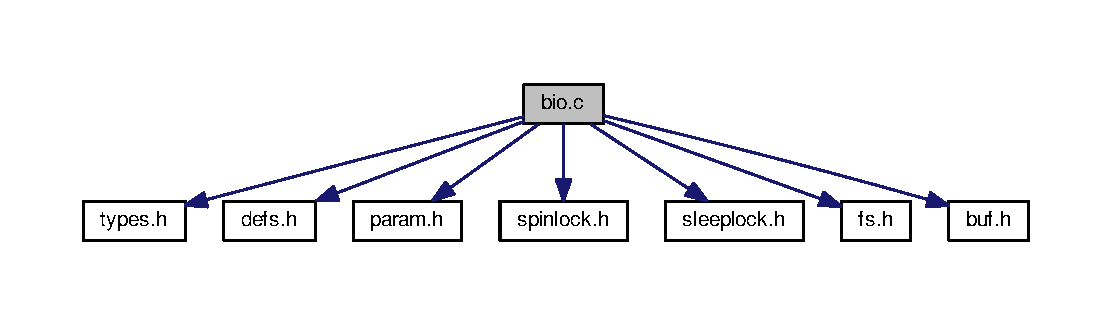
\includegraphics[width=350pt]{d9/d72/bio_8c__incl}
\end{center}
\end{figure}
\subsection*{Functions}
\begin{DoxyCompactItemize}
\item 
void \hyperlink{bio_8c_a53cca0ddc98c5f1de37124eca2575a59}{binit} (void)
\item 
struct \hyperlink{structbuf}{buf} $\ast$ \hyperlink{bio_8c_ae000984516278965dde3d125affd086c}{bread} (\hyperlink{types_8h_a91ad9478d81a7aaf2593e8d9c3d06a14}{uint} dev, \hyperlink{types_8h_a91ad9478d81a7aaf2593e8d9c3d06a14}{uint} blockno)
\item 
void \hyperlink{bio_8c_a63c899c13b176ddf80064d32225e1298}{bwrite} (struct \hyperlink{structbuf}{buf} $\ast$b)
\item 
void \hyperlink{bio_8c_ab5335aeb503731104314321a78a6d727}{brelse} (struct \hyperlink{structbuf}{buf} $\ast$b)
\end{DoxyCompactItemize}
\subsection*{Variables}
\begin{DoxyCompactItemize}
\item 
\begin{tabbing}
xx\=xx\=xx\=xx\=xx\=xx\=xx\=xx\=xx\=\kill
struct \{\\
\>struct \hyperlink{structspinlock}{spinlock} \hyperlink{bio_8c_ab28e82cd5dda7d960095706a3ea20572}{lock}\\
\>struct \hyperlink{structbuf}{buf} \hyperlink{bio_8c_a72ee90c61d41547b10a533c219e081c6}{buf} \mbox{[}\hyperlink{param_8h_ad51e2f8dffd163c263ec676a268d0f0a}{NBUF}\mbox{]}\\
\>struct \hyperlink{structbuf}{buf} \hyperlink{bio_8c_aa6e692c16f1b909f5cb2a1832cf43430}{head}\\
\} \hyperlink{bio_8c_a8c840c340a1233a78bdb2af607bbbcfc}{bcache}\\

\end{tabbing}\end{DoxyCompactItemize}


\subsection{Function Documentation}
\index{bio.\+c@{bio.\+c}!binit@{binit}}
\index{binit@{binit}!bio.\+c@{bio.\+c}}
\subsubsection[{\texorpdfstring{binit(void)}{binit(void)}}]{\setlength{\rightskip}{0pt plus 5cm}void binit (
\begin{DoxyParamCaption}
\item[{void}]{}
\end{DoxyParamCaption}
)}\hypertarget{bio_8c_a53cca0ddc98c5f1de37124eca2575a59}{}\label{bio_8c_a53cca0ddc98c5f1de37124eca2575a59}


Here is the call graph for this function\+:\nopagebreak
\begin{figure}[H]
\begin{center}
\leavevmode
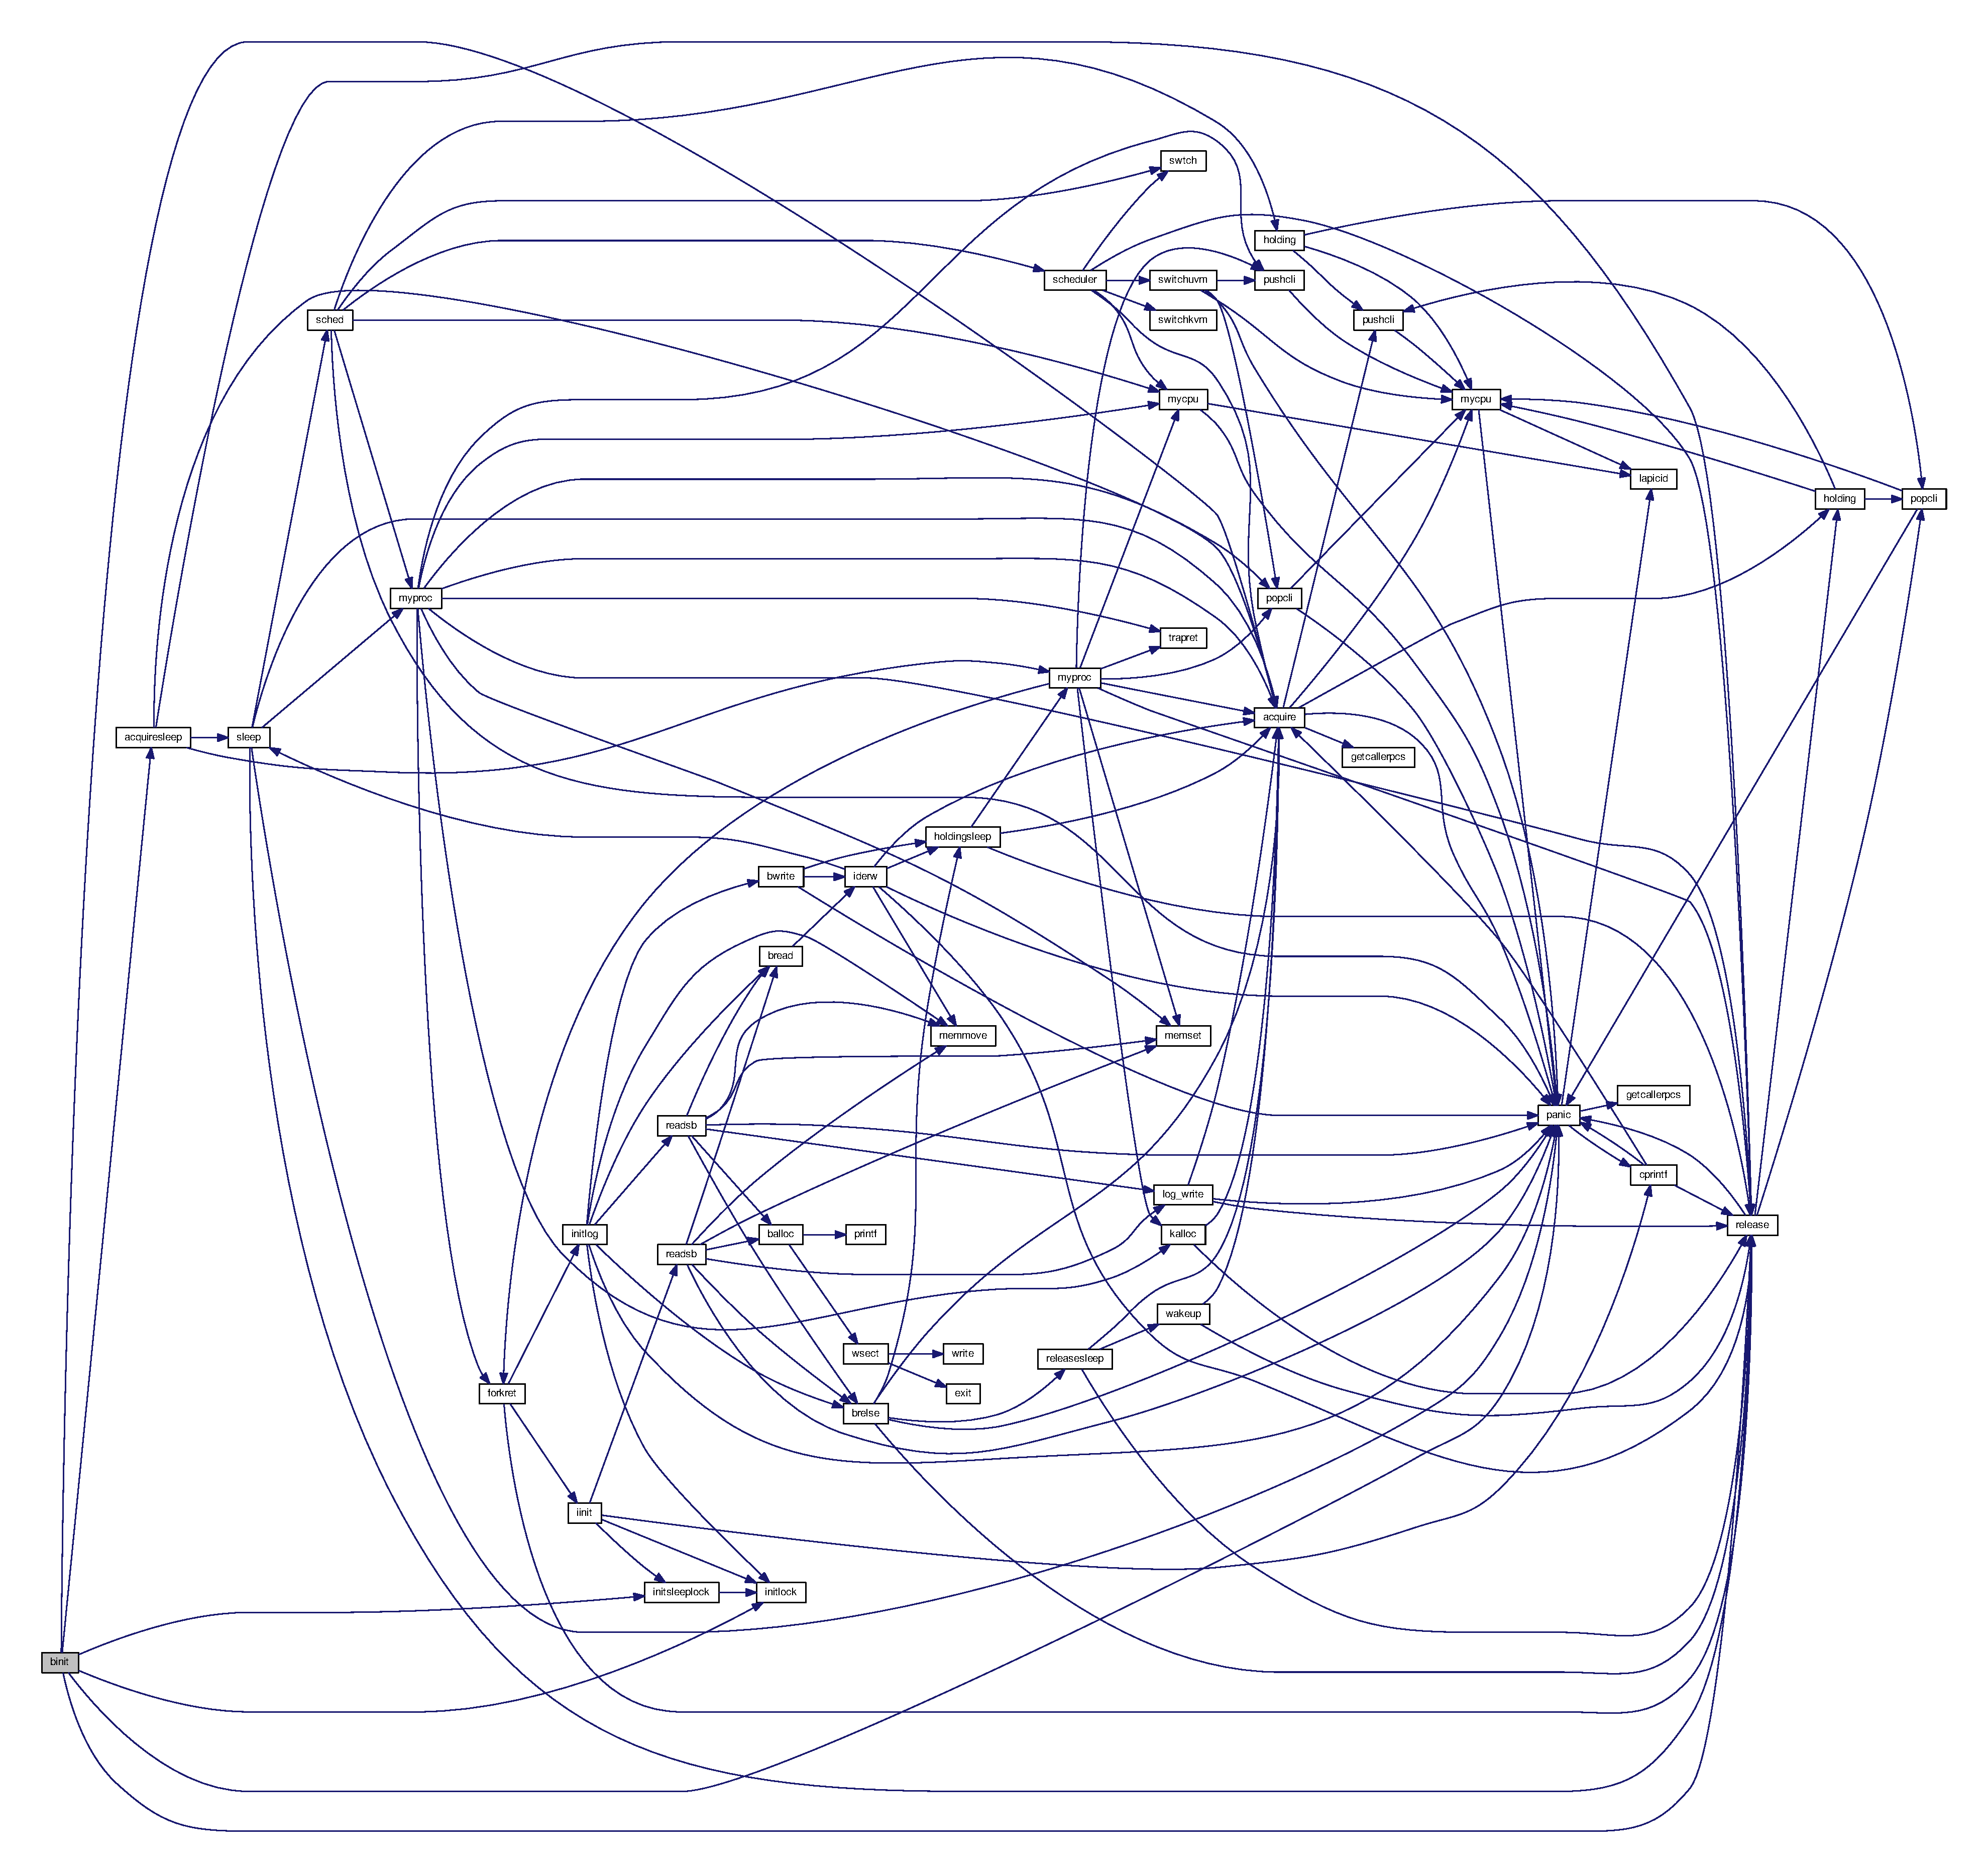
\includegraphics[width=350pt]{dc/de6/bio_8c_a53cca0ddc98c5f1de37124eca2575a59_cgraph}
\end{center}
\end{figure}


\index{bio.\+c@{bio.\+c}!bread@{bread}}
\index{bread@{bread}!bio.\+c@{bio.\+c}}
\subsubsection[{\texorpdfstring{bread(uint dev, uint blockno)}{bread(uint dev, uint blockno)}}]{\setlength{\rightskip}{0pt plus 5cm}struct {\bf buf}$\ast$ bread (
\begin{DoxyParamCaption}
\item[{{\bf uint}}]{dev, }
\item[{{\bf uint}}]{blockno}
\end{DoxyParamCaption}
)}\hypertarget{bio_8c_ae000984516278965dde3d125affd086c}{}\label{bio_8c_ae000984516278965dde3d125affd086c}


Here is the call graph for this function\+:\nopagebreak
\begin{figure}[H]
\begin{center}
\leavevmode
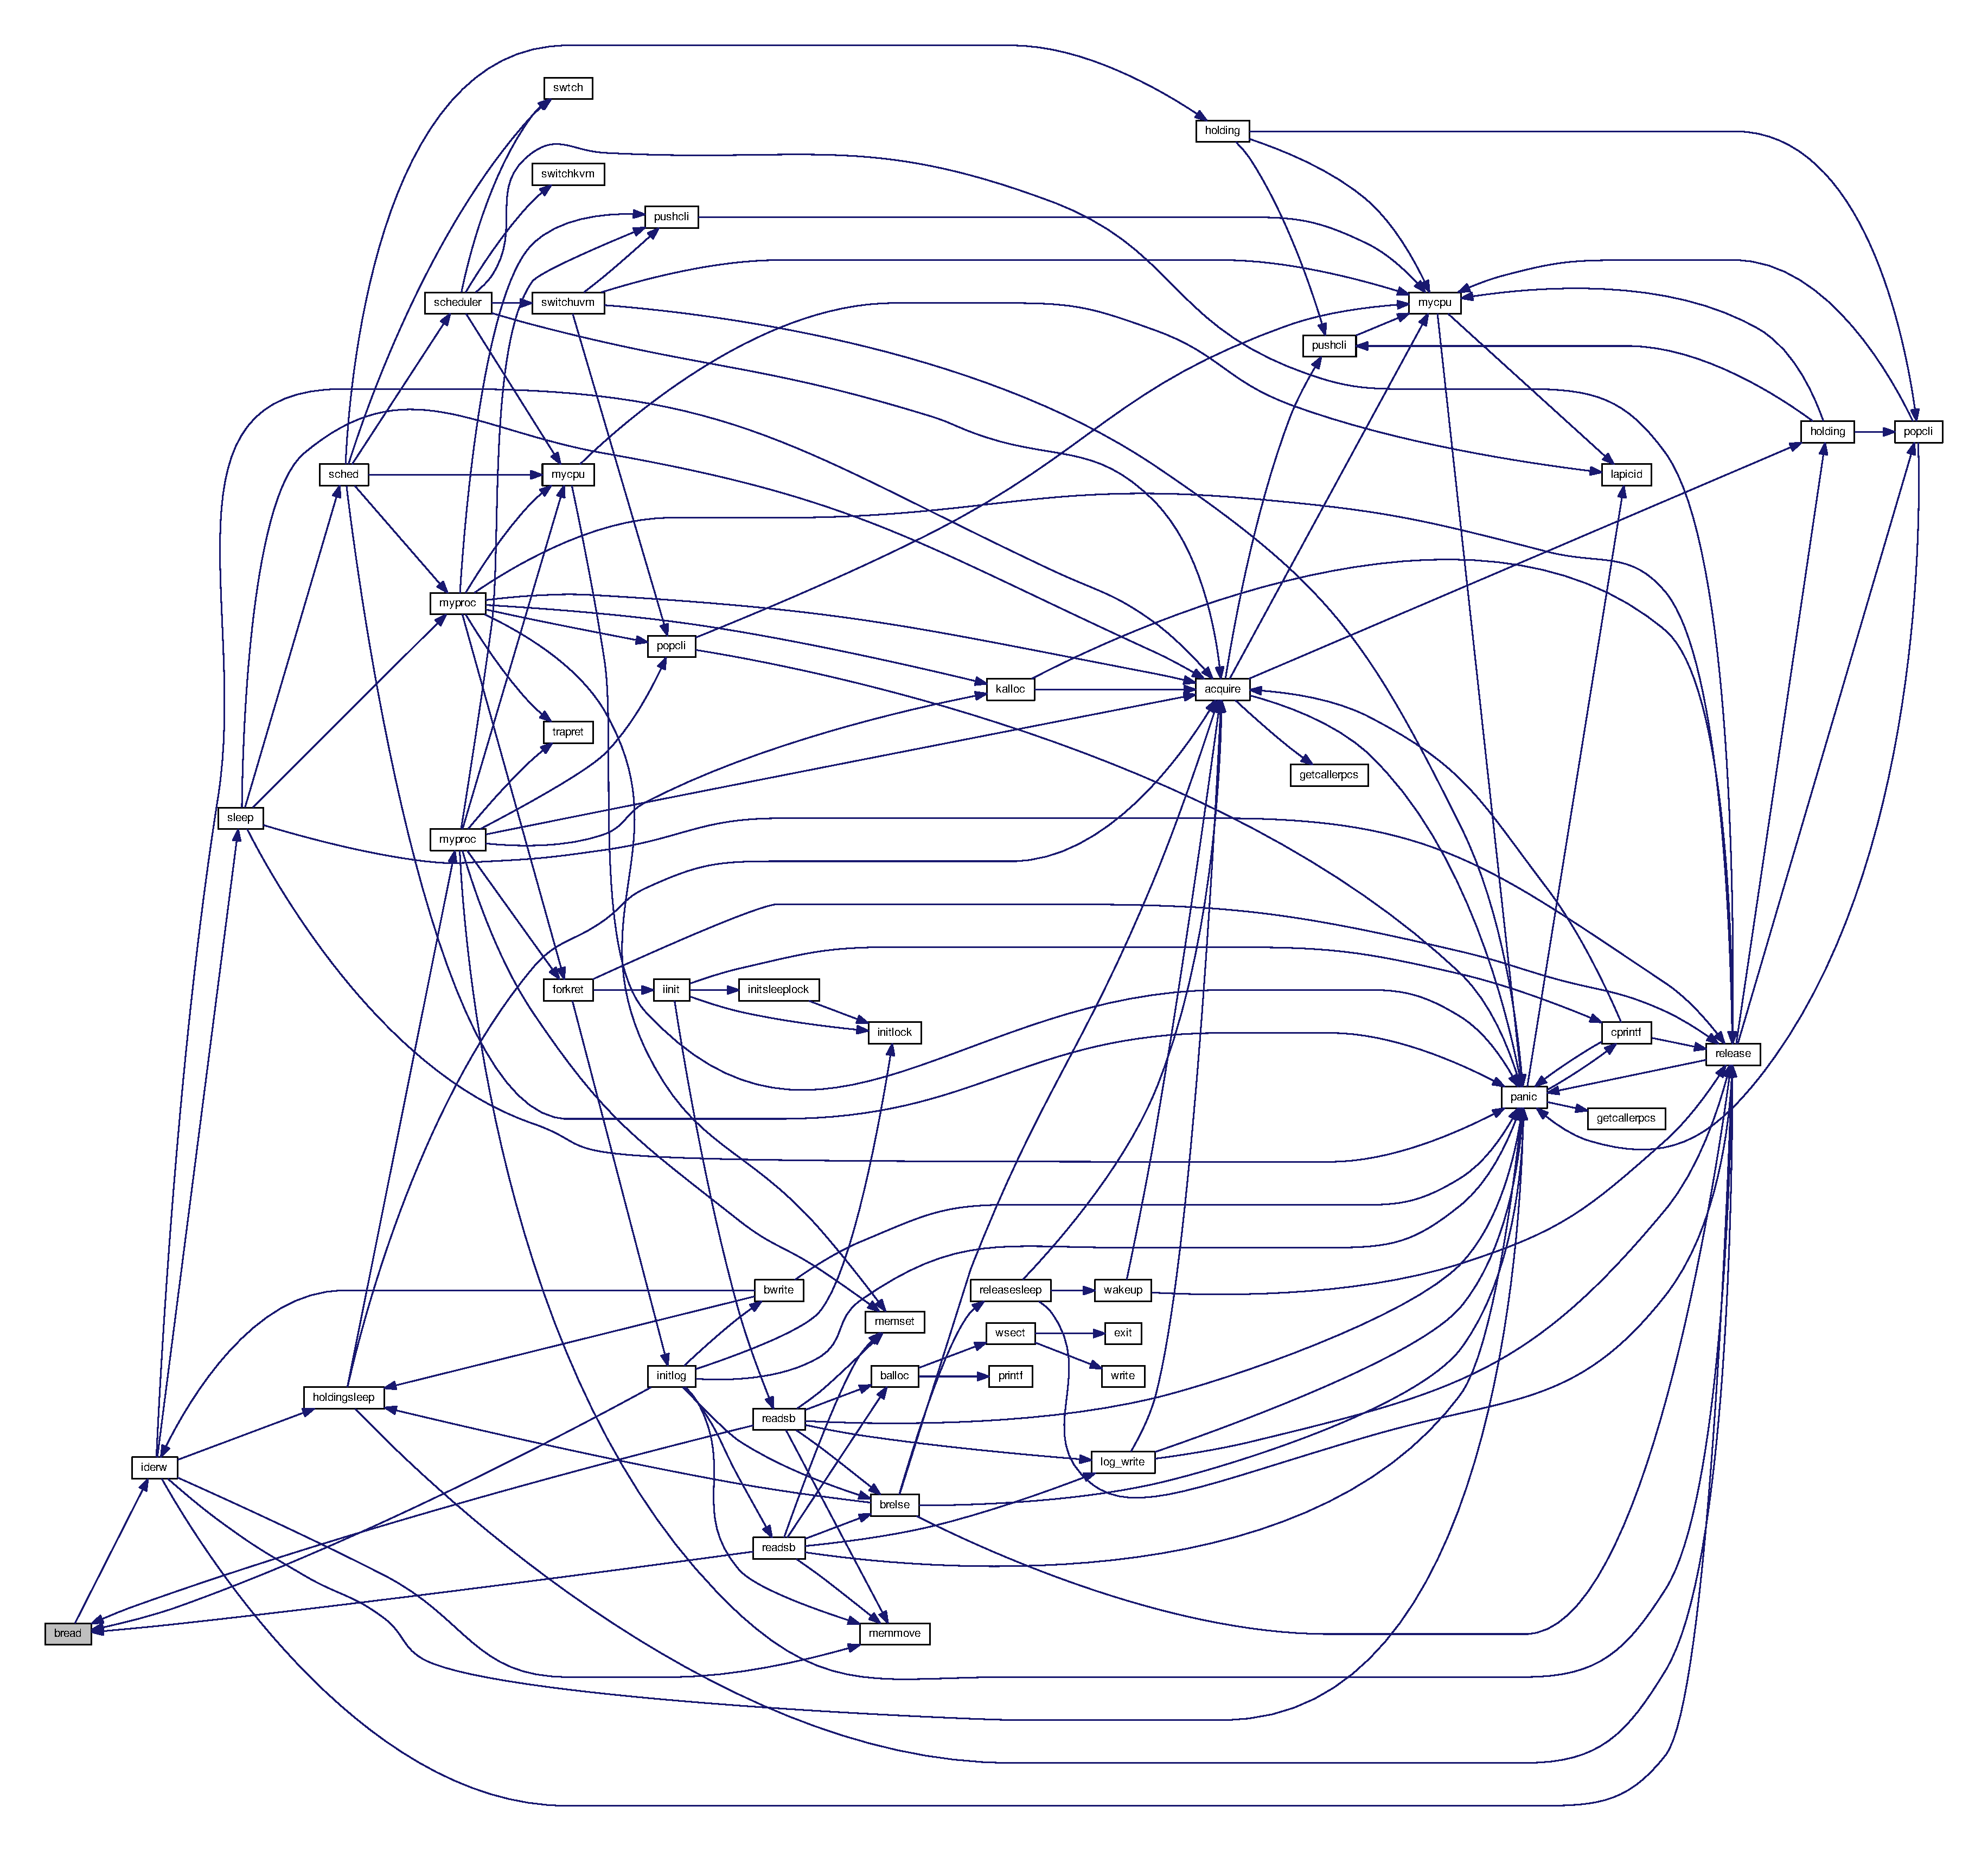
\includegraphics[width=350pt]{dc/de6/bio_8c_ae000984516278965dde3d125affd086c_cgraph}
\end{center}
\end{figure}




Here is the caller graph for this function\+:\nopagebreak
\begin{figure}[H]
\begin{center}
\leavevmode
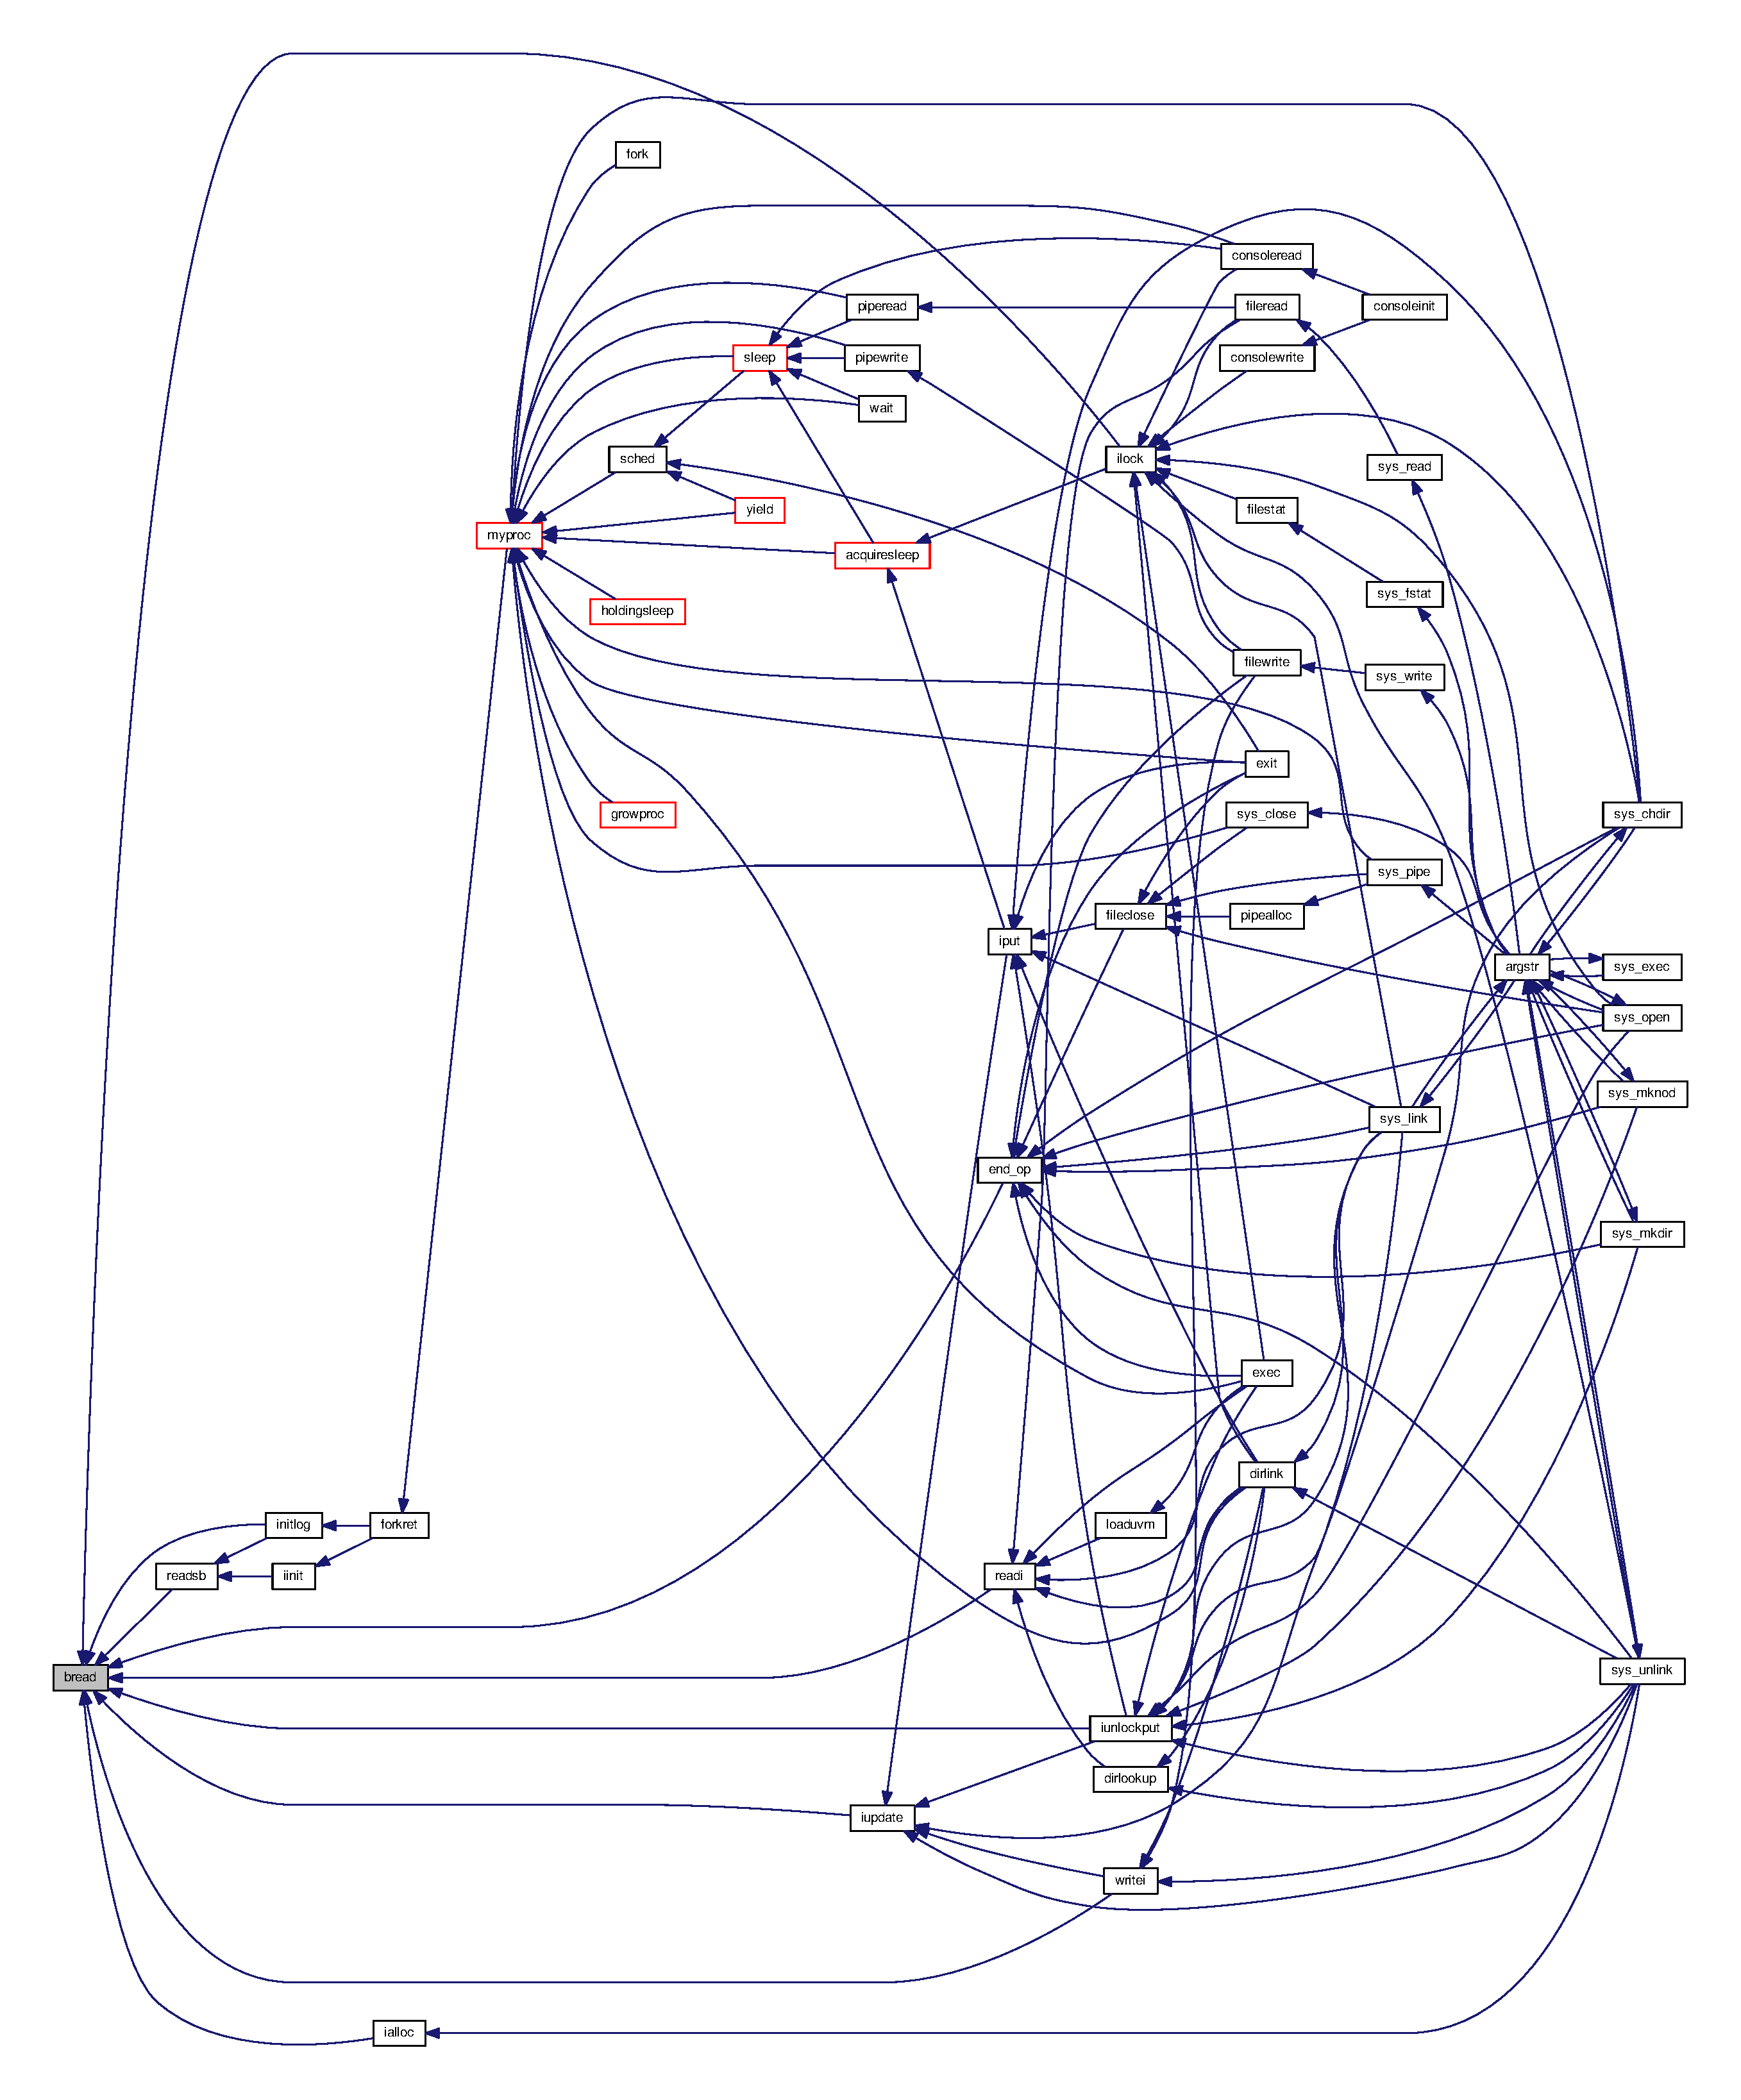
\includegraphics[width=350pt]{dc/de6/bio_8c_ae000984516278965dde3d125affd086c_icgraph}
\end{center}
\end{figure}


\index{bio.\+c@{bio.\+c}!brelse@{brelse}}
\index{brelse@{brelse}!bio.\+c@{bio.\+c}}
\subsubsection[{\texorpdfstring{brelse(struct buf $\ast$b)}{brelse(struct buf *b)}}]{\setlength{\rightskip}{0pt plus 5cm}void brelse (
\begin{DoxyParamCaption}
\item[{struct {\bf buf} $\ast$}]{b}
\end{DoxyParamCaption}
)}\hypertarget{bio_8c_ab5335aeb503731104314321a78a6d727}{}\label{bio_8c_ab5335aeb503731104314321a78a6d727}


Here is the call graph for this function\+:\nopagebreak
\begin{figure}[H]
\begin{center}
\leavevmode
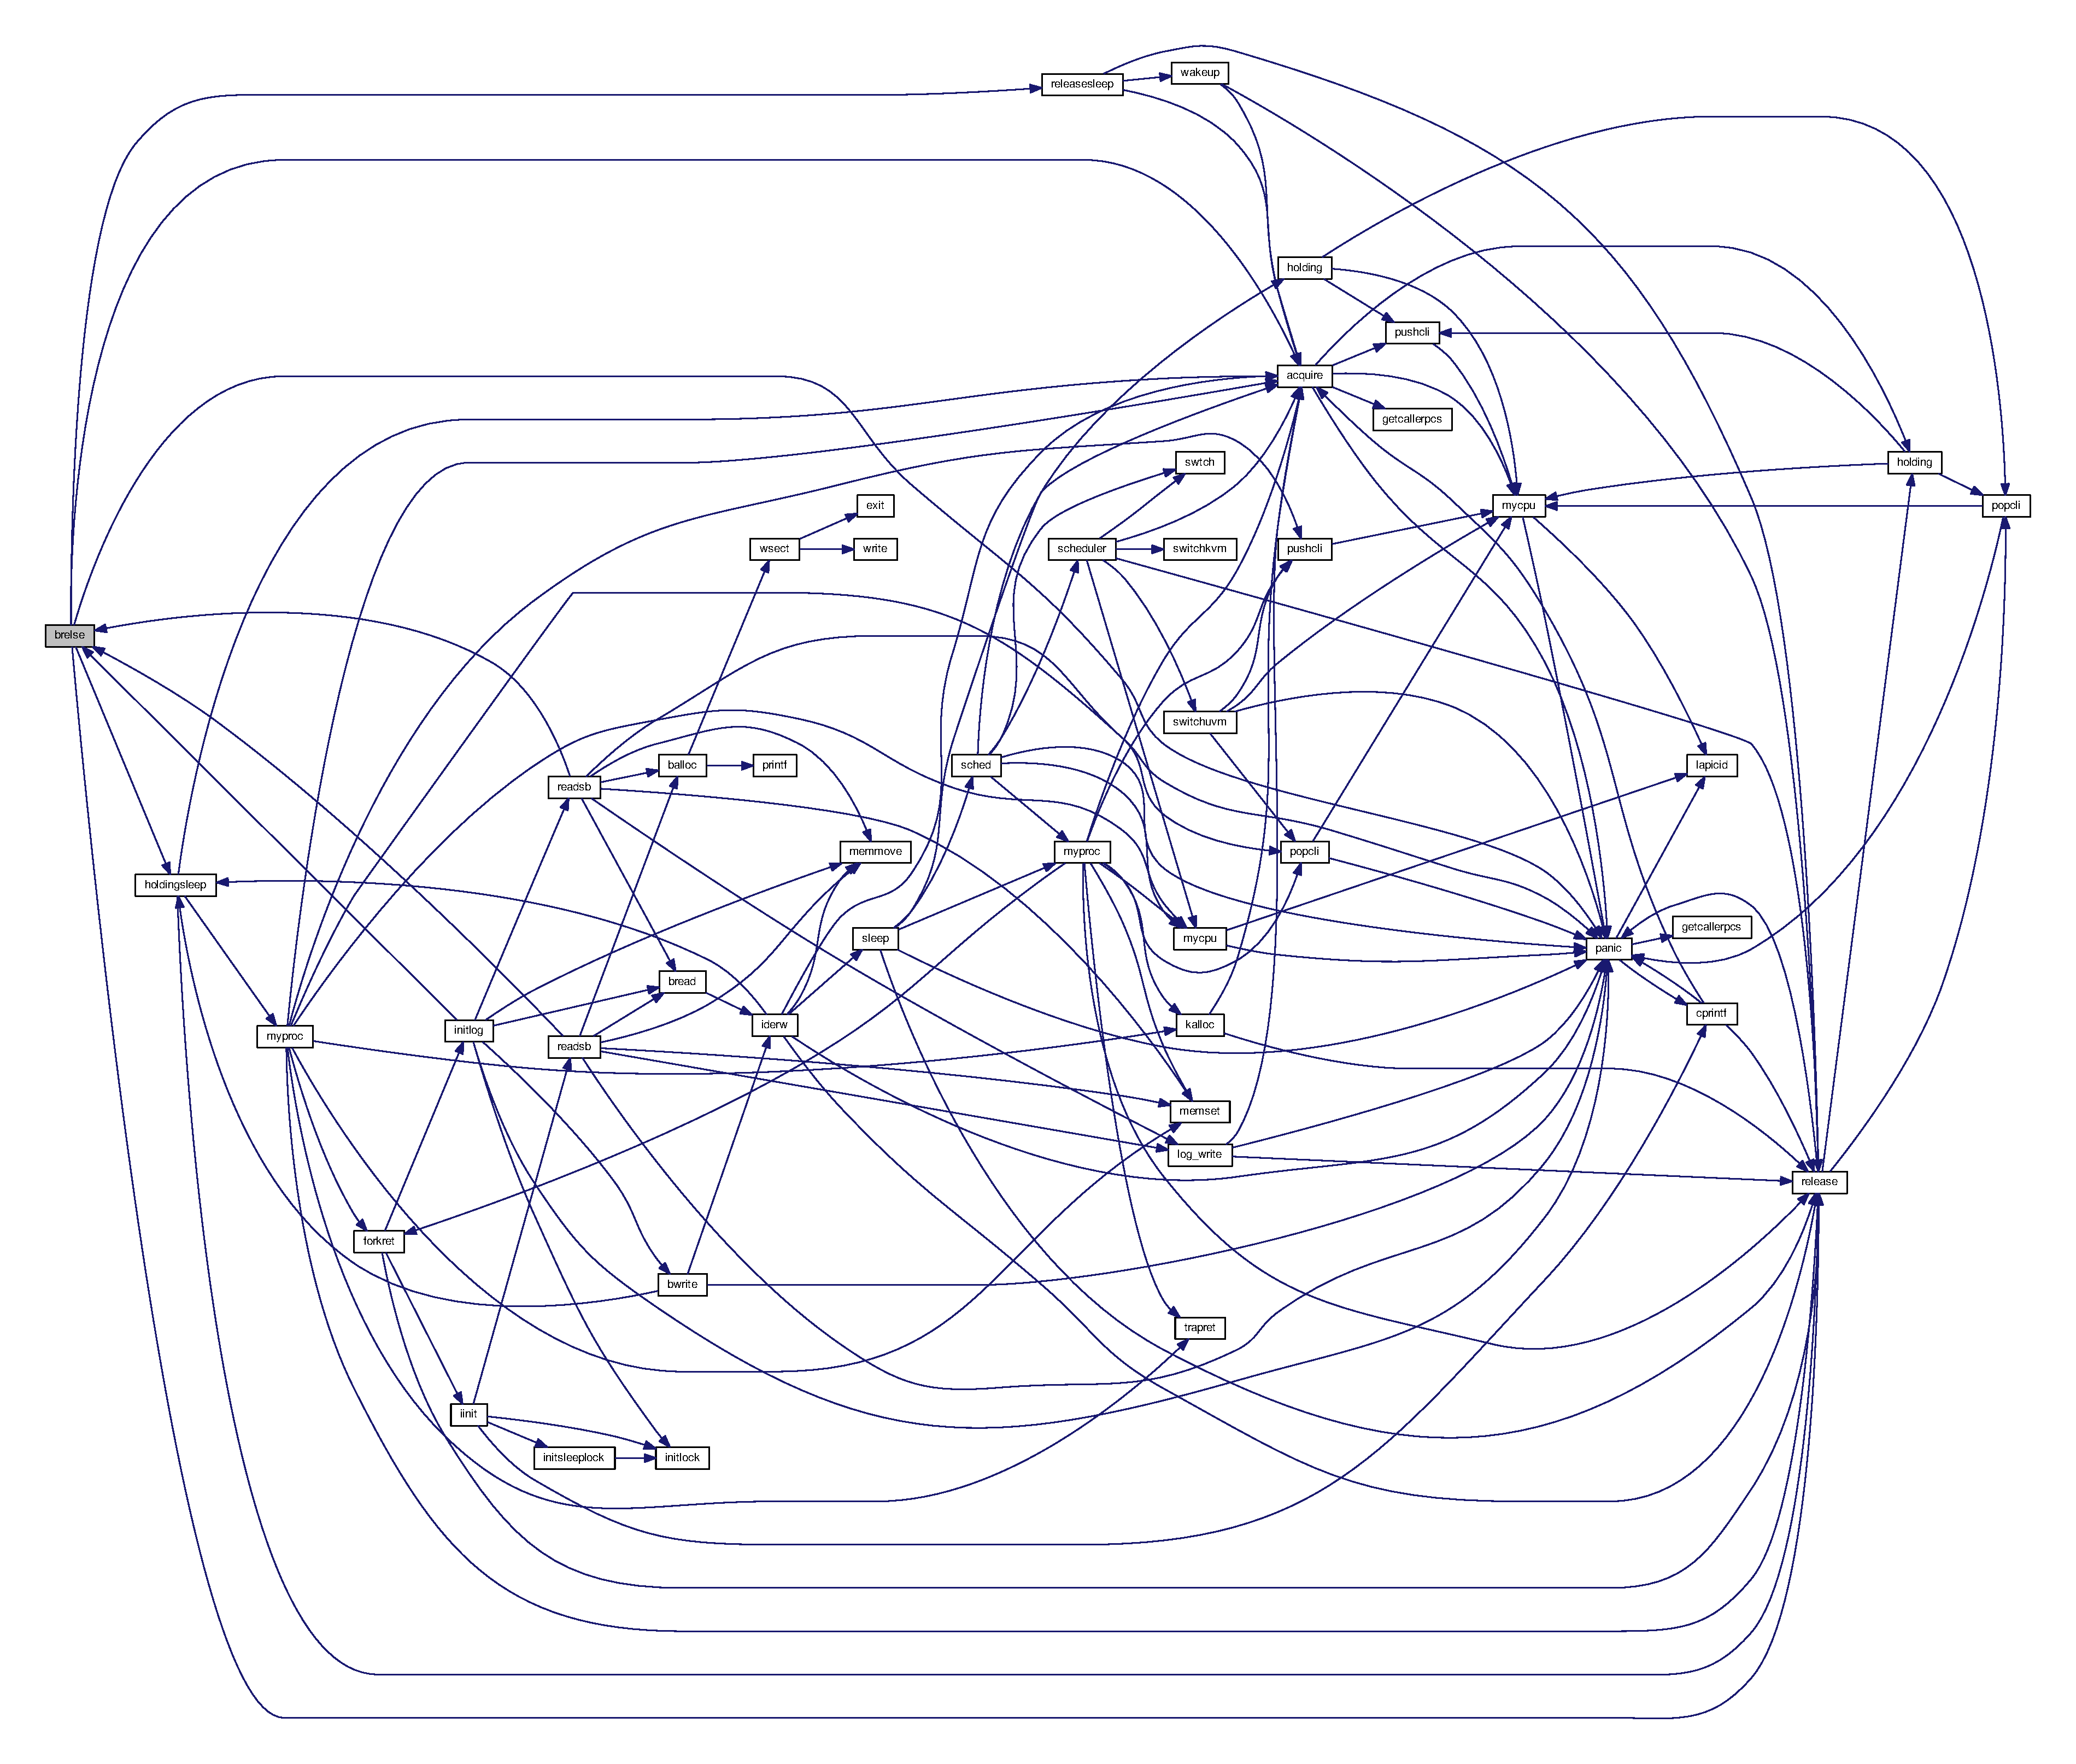
\includegraphics[width=350pt]{dc/de6/bio_8c_ab5335aeb503731104314321a78a6d727_cgraph}
\end{center}
\end{figure}




Here is the caller graph for this function\+:\nopagebreak
\begin{figure}[H]
\begin{center}
\leavevmode
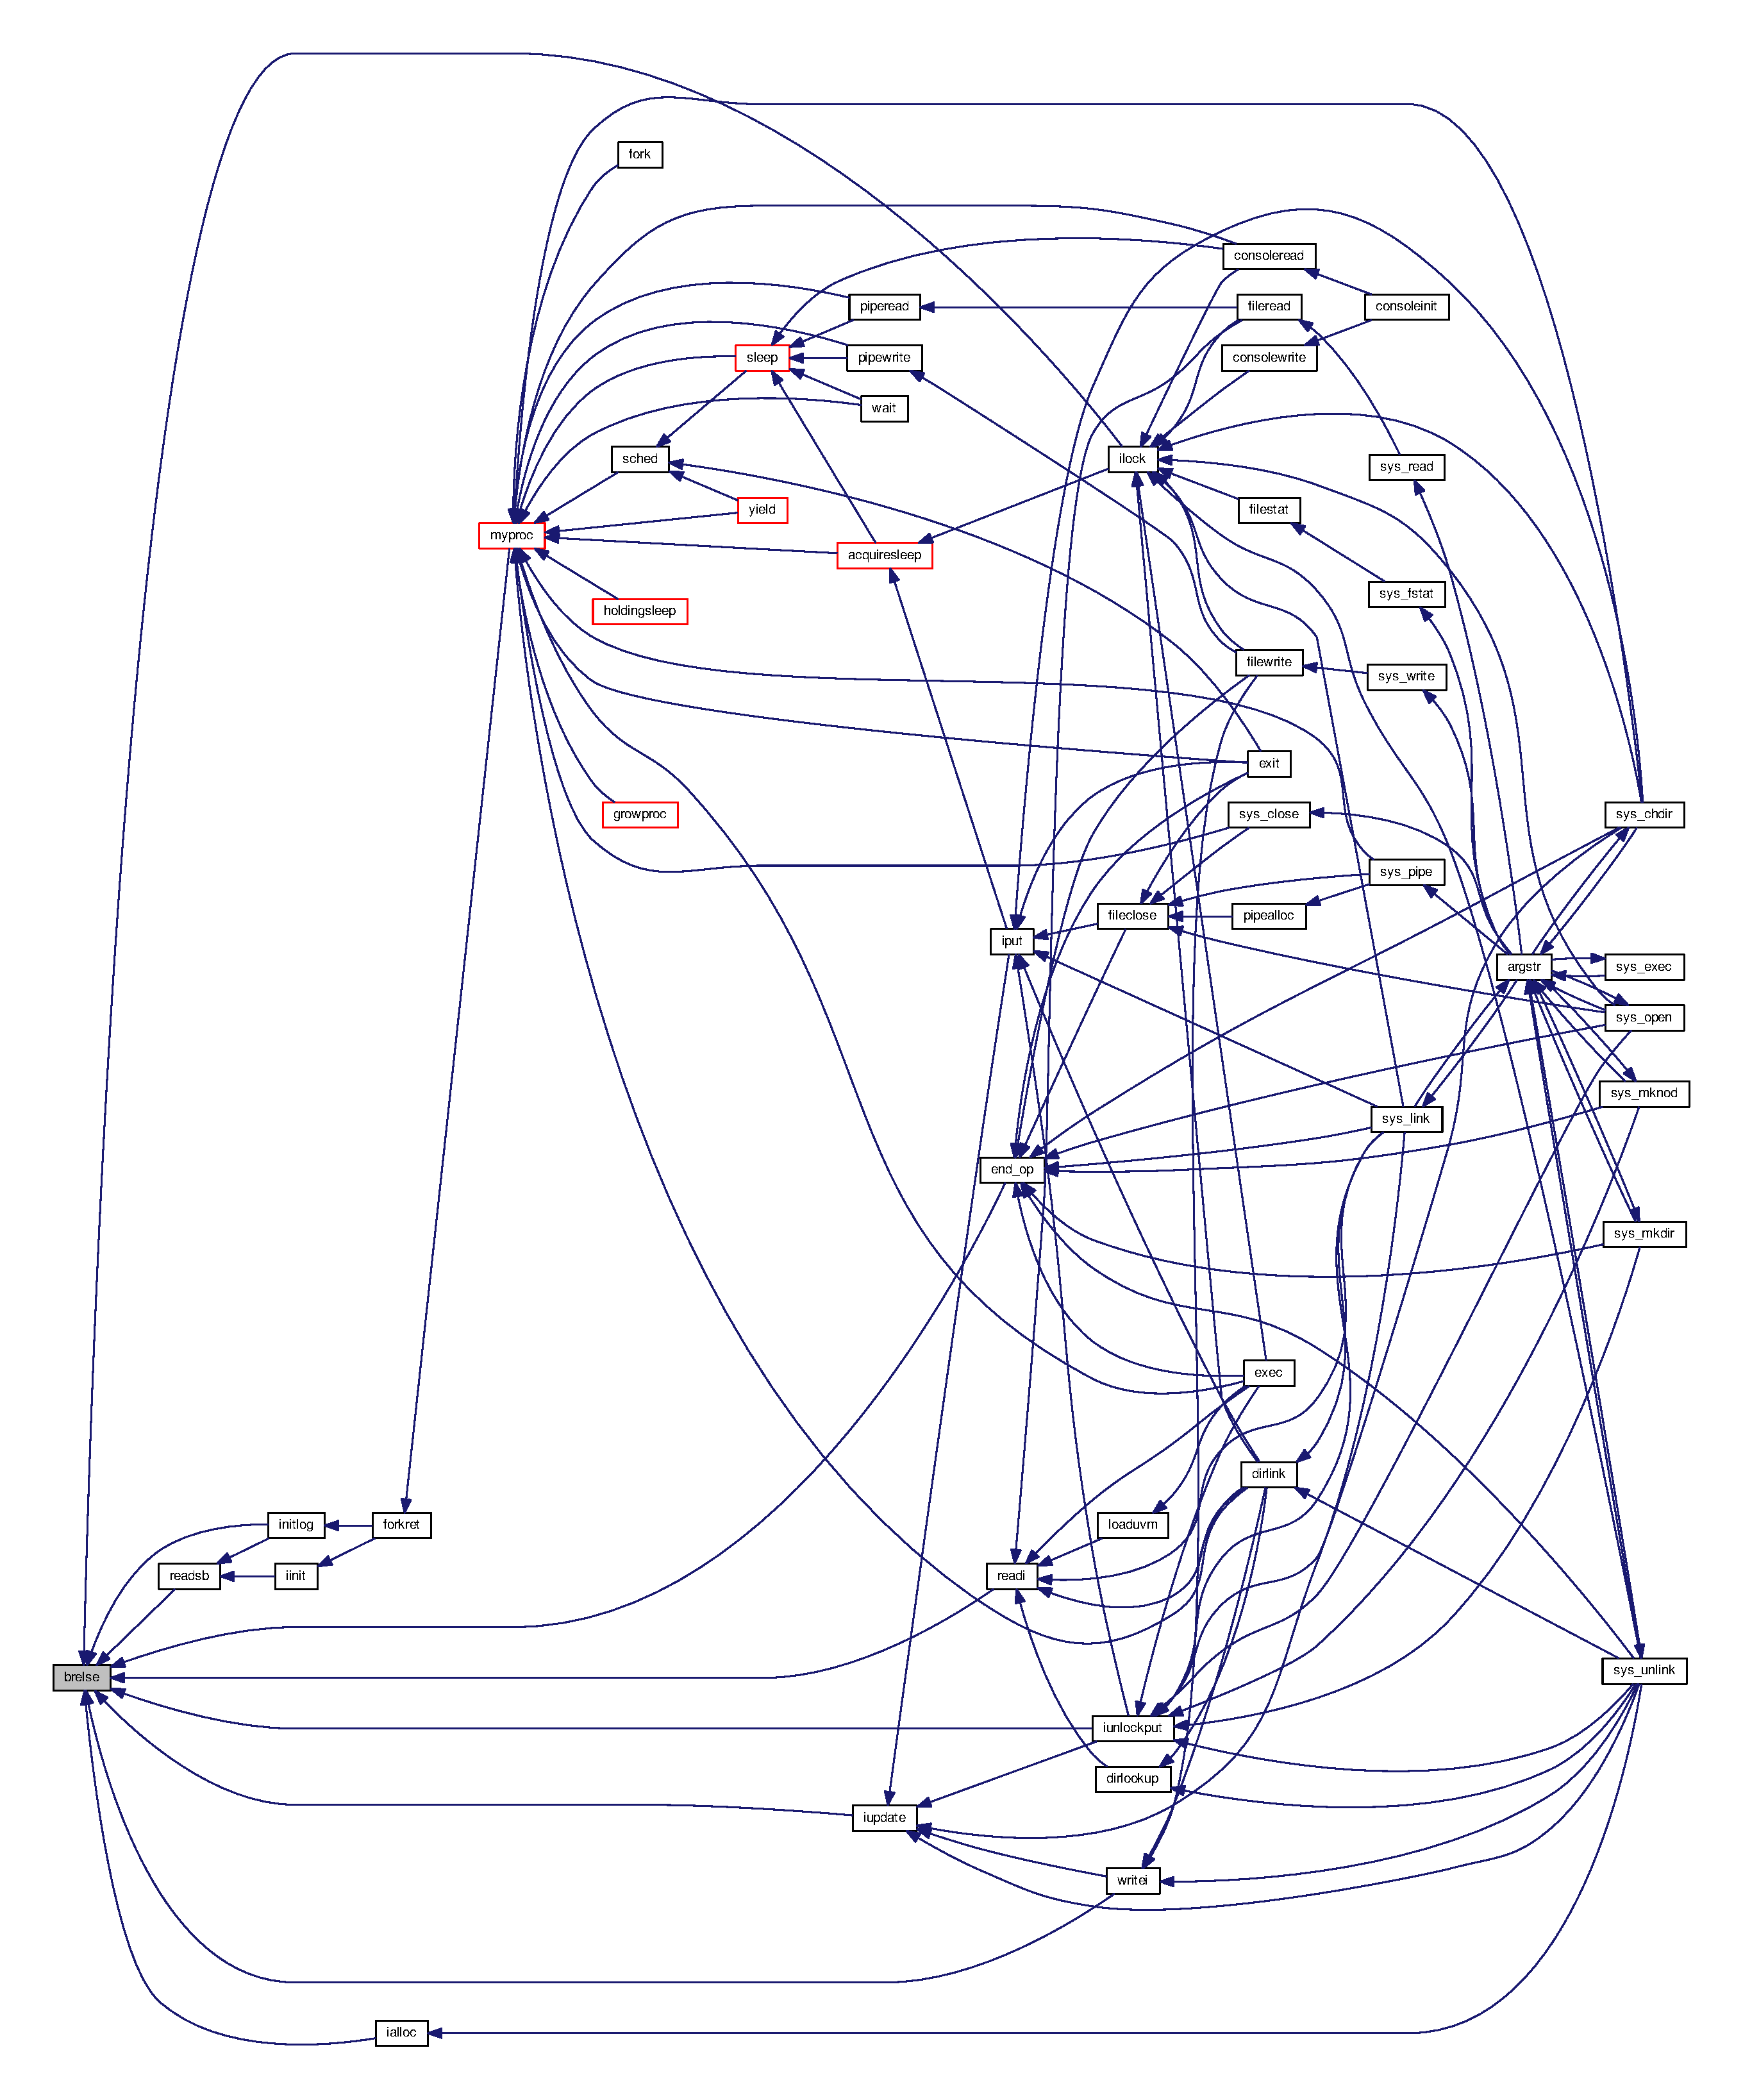
\includegraphics[width=350pt]{dc/de6/bio_8c_ab5335aeb503731104314321a78a6d727_icgraph}
\end{center}
\end{figure}


\index{bio.\+c@{bio.\+c}!bwrite@{bwrite}}
\index{bwrite@{bwrite}!bio.\+c@{bio.\+c}}
\subsubsection[{\texorpdfstring{bwrite(struct buf $\ast$b)}{bwrite(struct buf *b)}}]{\setlength{\rightskip}{0pt plus 5cm}void bwrite (
\begin{DoxyParamCaption}
\item[{struct {\bf buf} $\ast$}]{b}
\end{DoxyParamCaption}
)}\hypertarget{bio_8c_a63c899c13b176ddf80064d32225e1298}{}\label{bio_8c_a63c899c13b176ddf80064d32225e1298}


Here is the call graph for this function\+:\nopagebreak
\begin{figure}[H]
\begin{center}
\leavevmode
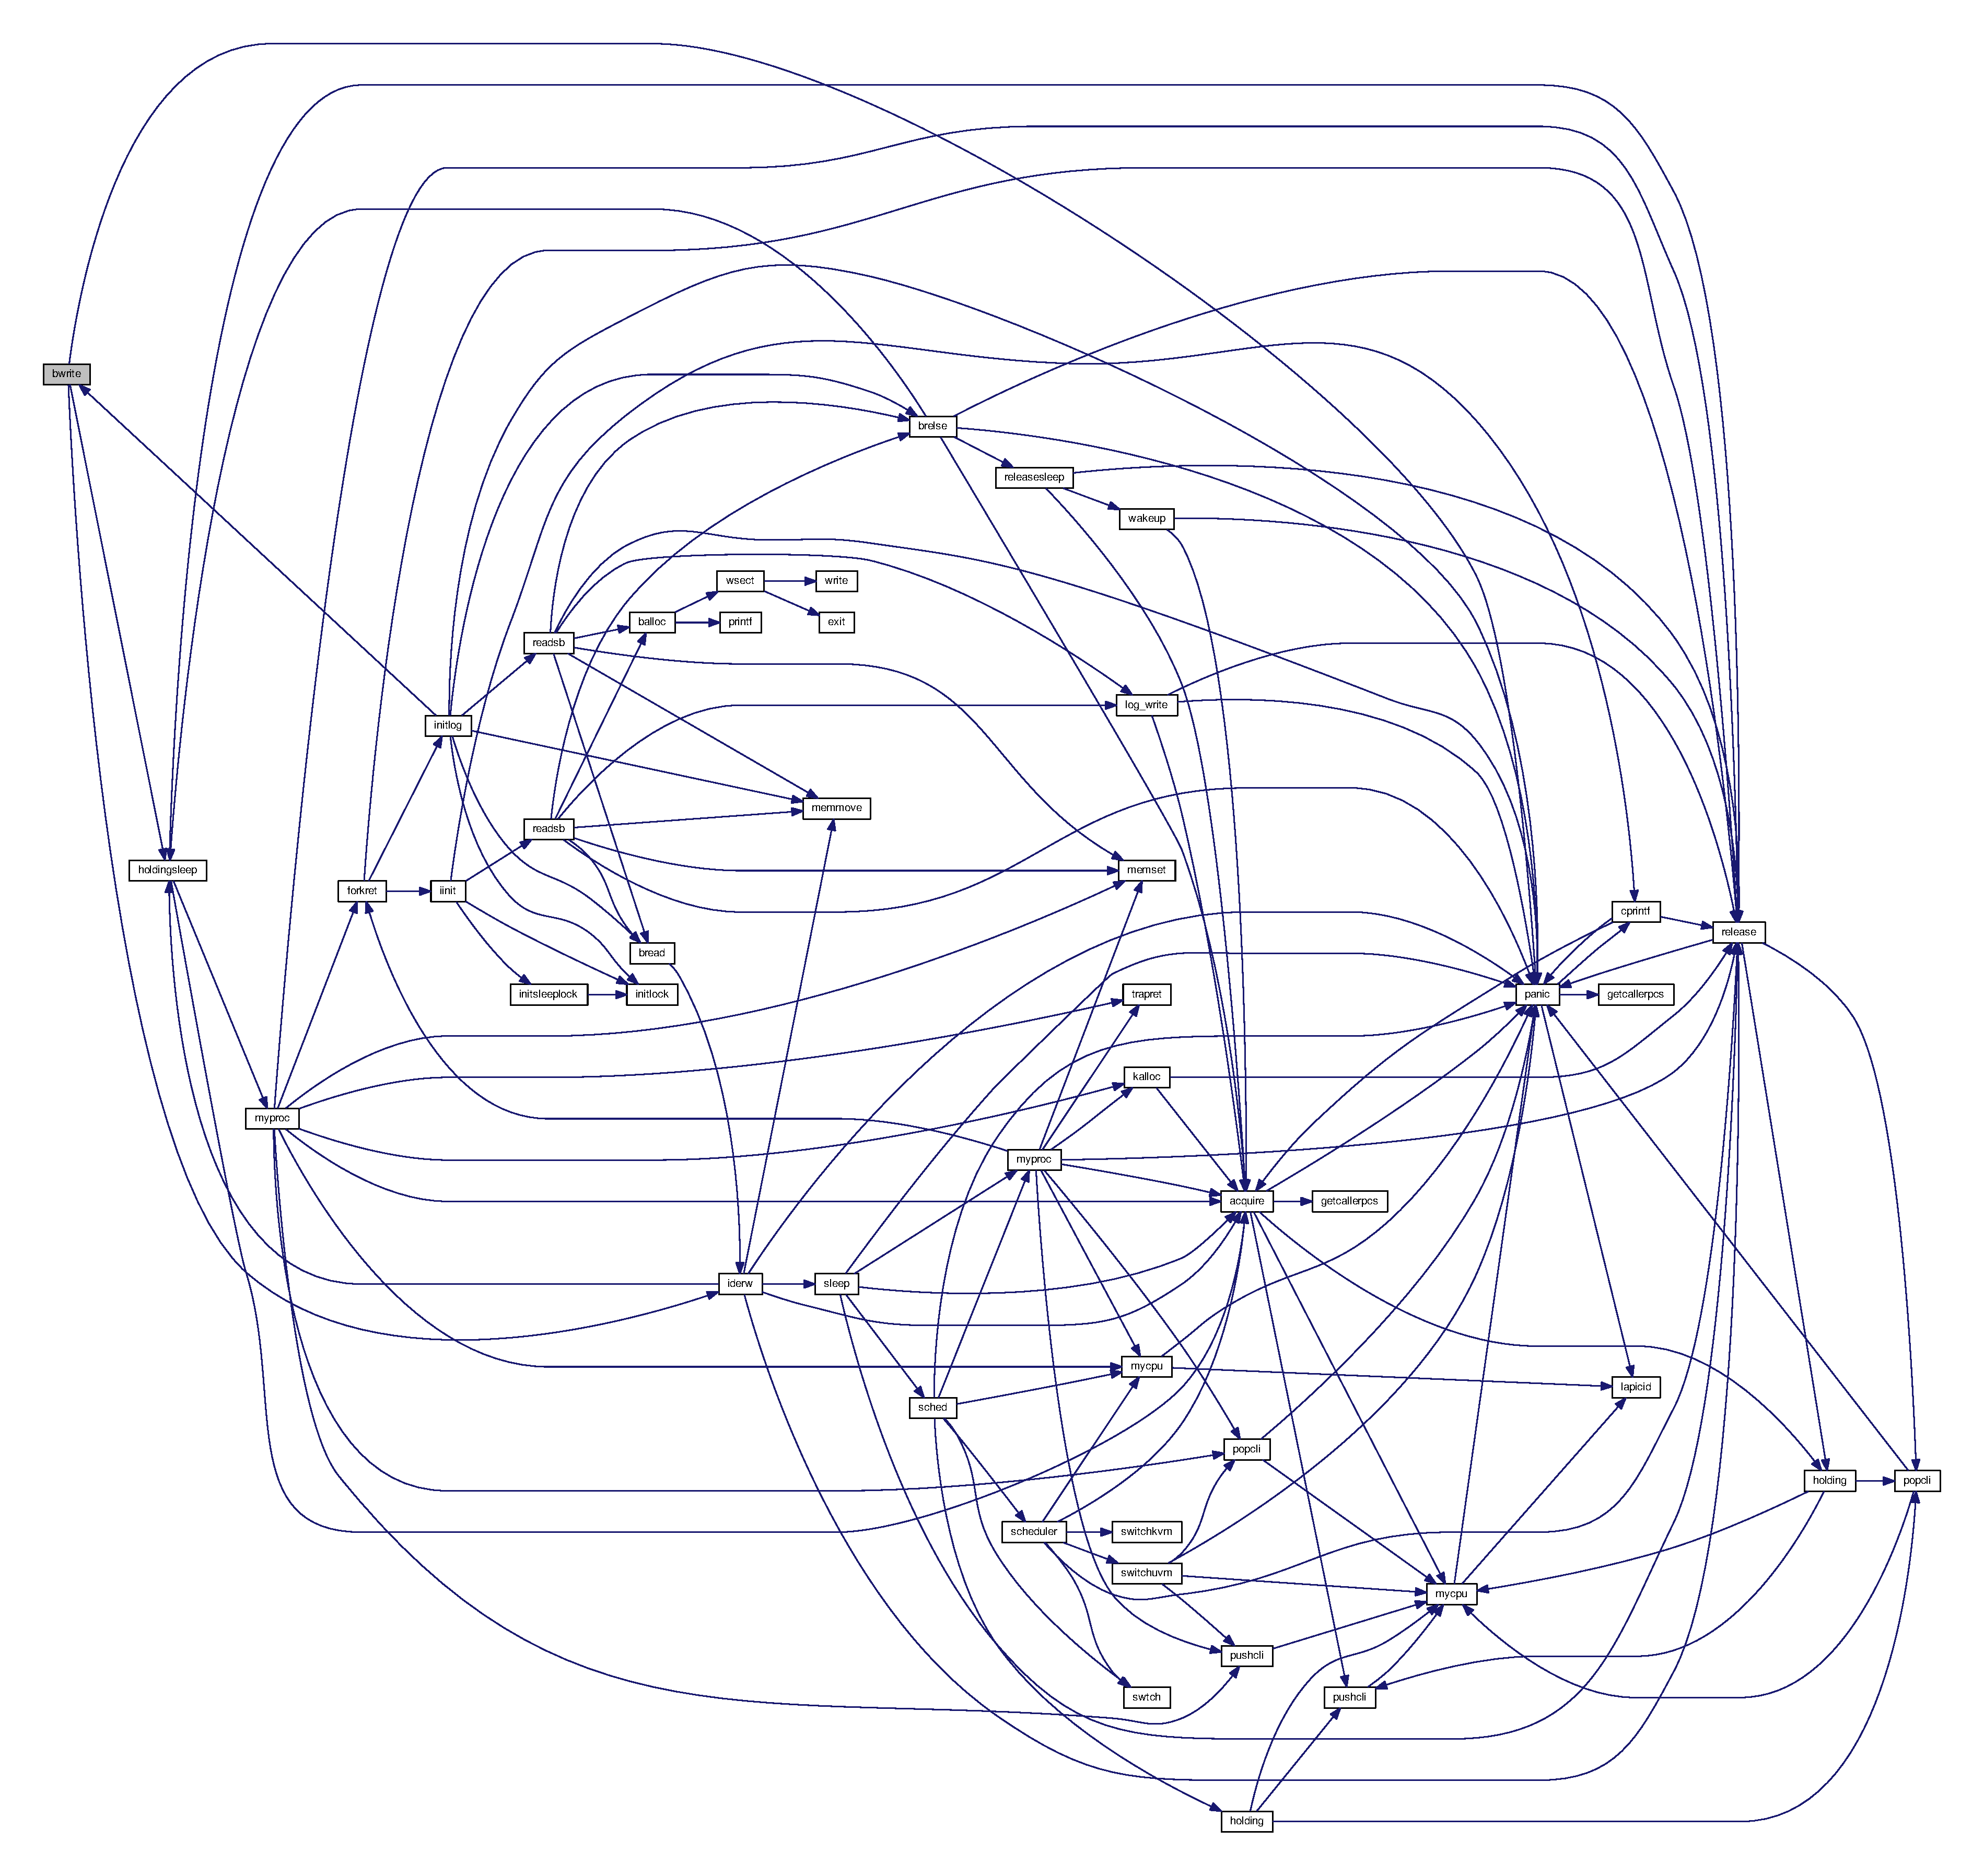
\includegraphics[width=350pt]{dc/de6/bio_8c_a63c899c13b176ddf80064d32225e1298_cgraph}
\end{center}
\end{figure}




Here is the caller graph for this function\+:\nopagebreak
\begin{figure}[H]
\begin{center}
\leavevmode
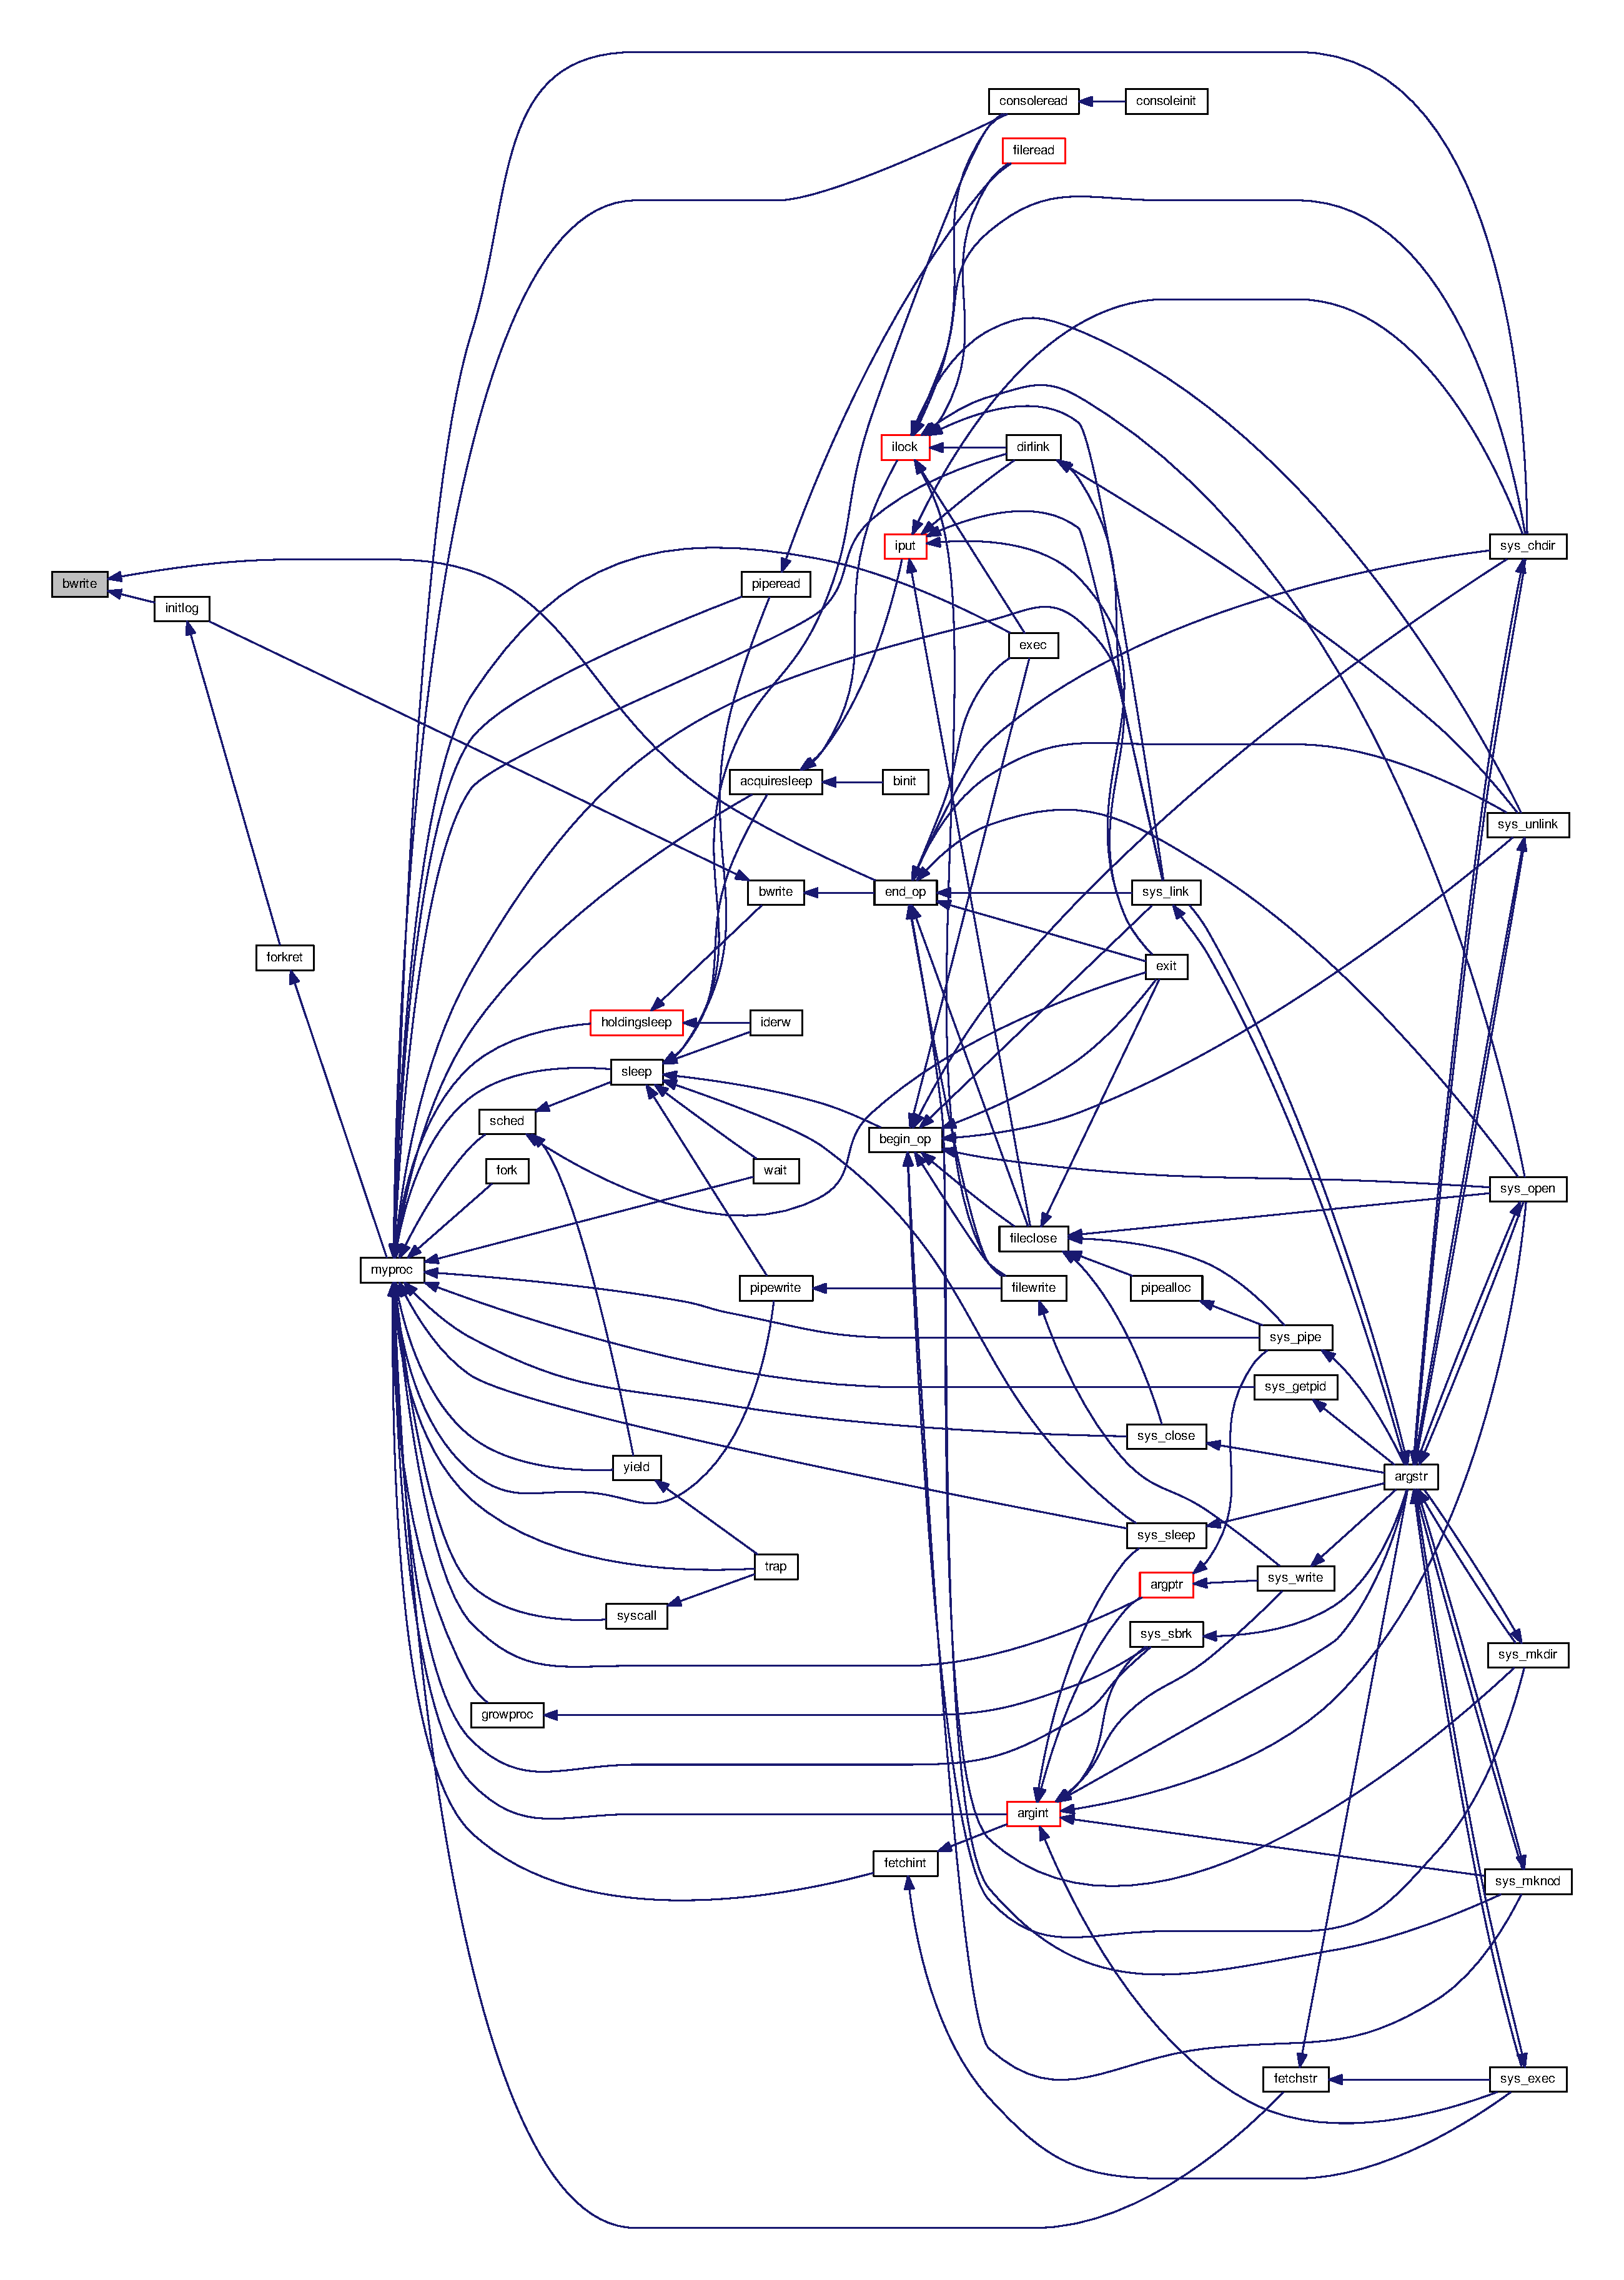
\includegraphics[width=350pt]{dc/de6/bio_8c_a63c899c13b176ddf80064d32225e1298_icgraph}
\end{center}
\end{figure}




\subsection{Variable Documentation}
\index{bio.\+c@{bio.\+c}!bcache@{bcache}}
\index{bcache@{bcache}!bio.\+c@{bio.\+c}}
\subsubsection[{\texorpdfstring{bcache}{bcache}}]{\setlength{\rightskip}{0pt plus 5cm}struct \{ ... \}   bcache}\hypertarget{bio_8c_a8c840c340a1233a78bdb2af607bbbcfc}{}\label{bio_8c_a8c840c340a1233a78bdb2af607bbbcfc}
\index{bio.\+c@{bio.\+c}!buf@{buf}}
\index{buf@{buf}!bio.\+c@{bio.\+c}}
\subsubsection[{\texorpdfstring{buf}{buf}}]{\setlength{\rightskip}{0pt plus 5cm}struct {\bf buf} {\bf buf}\mbox{[}{\bf N\+B\+UF}\mbox{]}}\hypertarget{bio_8c_a72ee90c61d41547b10a533c219e081c6}{}\label{bio_8c_a72ee90c61d41547b10a533c219e081c6}
\index{bio.\+c@{bio.\+c}!head@{head}}
\index{head@{head}!bio.\+c@{bio.\+c}}
\subsubsection[{\texorpdfstring{head}{head}}]{\setlength{\rightskip}{0pt plus 5cm}struct {\bf buf} head}\hypertarget{bio_8c_aa6e692c16f1b909f5cb2a1832cf43430}{}\label{bio_8c_aa6e692c16f1b909f5cb2a1832cf43430}
\index{bio.\+c@{bio.\+c}!lock@{lock}}
\index{lock@{lock}!bio.\+c@{bio.\+c}}
\subsubsection[{\texorpdfstring{lock}{lock}}]{\setlength{\rightskip}{0pt plus 5cm}struct {\bf spinlock} lock}\hypertarget{bio_8c_ab28e82cd5dda7d960095706a3ea20572}{}\label{bio_8c_ab28e82cd5dda7d960095706a3ea20572}

\hypertarget{bio_8d}{}\section{bio.\+d File Reference}
\label{bio_8d}\index{bio.\+d@{bio.\+d}}

\hypertarget{bootasm_8d}{}\section{bootasm.\+d File Reference}
\label{bootasm_8d}\index{bootasm.\+d@{bootasm.\+d}}

\hypertarget{bootmain_8c}{}\section{bootmain.\+c File Reference}
\label{bootmain_8c}\index{bootmain.\+c@{bootmain.\+c}}
{\ttfamily \#include \char`\"{}types.\+h\char`\"{}}\\*
{\ttfamily \#include \char`\"{}elf.\+h\char`\"{}}\\*
{\ttfamily \#include \char`\"{}x86.\+h\char`\"{}}\\*
{\ttfamily \#include \char`\"{}memlayout.\+h\char`\"{}}\\*
Include dependency graph for bootmain.\+c\+:\nopagebreak
\begin{figure}[H]
\begin{center}
\leavevmode
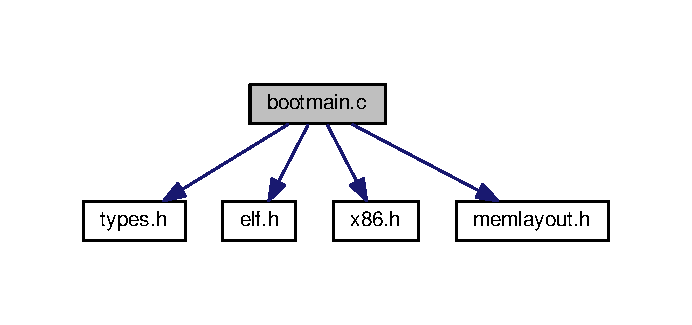
\includegraphics[width=332pt]{de/d8f/bootmain_8c__incl}
\end{center}
\end{figure}
\subsection*{Macros}
\begin{DoxyCompactItemize}
\item 
\#define \hyperlink{bootmain_8c_af69dd8b281718a66b3e7a65250d24419}{S\+E\+C\+T\+S\+I\+ZE}~512
\end{DoxyCompactItemize}
\subsection*{Functions}
\begin{DoxyCompactItemize}
\item 
void \hyperlink{bootmain_8c_af8097ce47ae21ccad1b0afd6f48ef62c}{readseg} (\hyperlink{types_8h_a65f85814a8290f9797005d3b28e7e5fc}{uchar} $\ast$, \hyperlink{types_8h_a91ad9478d81a7aaf2593e8d9c3d06a14}{uint}, \hyperlink{types_8h_a91ad9478d81a7aaf2593e8d9c3d06a14}{uint})
\item 
void \hyperlink{bootmain_8c_a0d198d492591e1b70a8a12109408a7e4}{bootmain} (void)
\item 
void \hyperlink{bootmain_8c_a63222d4a07c38c198de5bd116a001935}{waitdisk} (void)
\item 
void \hyperlink{bootmain_8c_ae7ef59ffa082283b72c54e43b7a16351}{readsect} (void $\ast$dst, \hyperlink{types_8h_a91ad9478d81a7aaf2593e8d9c3d06a14}{uint} offset)
\end{DoxyCompactItemize}


\subsection{Macro Definition Documentation}
\index{bootmain.\+c@{bootmain.\+c}!S\+E\+C\+T\+S\+I\+ZE@{S\+E\+C\+T\+S\+I\+ZE}}
\index{S\+E\+C\+T\+S\+I\+ZE@{S\+E\+C\+T\+S\+I\+ZE}!bootmain.\+c@{bootmain.\+c}}
\subsubsection[{\texorpdfstring{S\+E\+C\+T\+S\+I\+ZE}{SECTSIZE}}]{\setlength{\rightskip}{0pt plus 5cm}\#define S\+E\+C\+T\+S\+I\+ZE~512}\hypertarget{bootmain_8c_af69dd8b281718a66b3e7a65250d24419}{}\label{bootmain_8c_af69dd8b281718a66b3e7a65250d24419}


\subsection{Function Documentation}
\index{bootmain.\+c@{bootmain.\+c}!bootmain@{bootmain}}
\index{bootmain@{bootmain}!bootmain.\+c@{bootmain.\+c}}
\subsubsection[{\texorpdfstring{bootmain(void)}{bootmain(void)}}]{\setlength{\rightskip}{0pt plus 5cm}void bootmain (
\begin{DoxyParamCaption}
\item[{void}]{}
\end{DoxyParamCaption}
)}\hypertarget{bootmain_8c_a0d198d492591e1b70a8a12109408a7e4}{}\label{bootmain_8c_a0d198d492591e1b70a8a12109408a7e4}


Here is the call graph for this function\+:\nopagebreak
\begin{figure}[H]
\begin{center}
\leavevmode
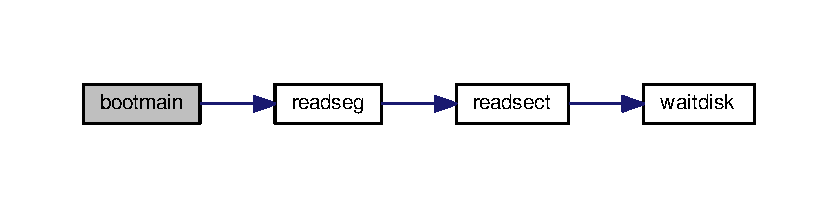
\includegraphics[width=350pt]{d5/dfc/bootmain_8c_a0d198d492591e1b70a8a12109408a7e4_cgraph}
\end{center}
\end{figure}


\index{bootmain.\+c@{bootmain.\+c}!readsect@{readsect}}
\index{readsect@{readsect}!bootmain.\+c@{bootmain.\+c}}
\subsubsection[{\texorpdfstring{readsect(void $\ast$dst, uint offset)}{readsect(void *dst, uint offset)}}]{\setlength{\rightskip}{0pt plus 5cm}void readsect (
\begin{DoxyParamCaption}
\item[{void $\ast$}]{dst, }
\item[{{\bf uint}}]{offset}
\end{DoxyParamCaption}
)}\hypertarget{bootmain_8c_ae7ef59ffa082283b72c54e43b7a16351}{}\label{bootmain_8c_ae7ef59ffa082283b72c54e43b7a16351}


Here is the call graph for this function\+:\nopagebreak
\begin{figure}[H]
\begin{center}
\leavevmode
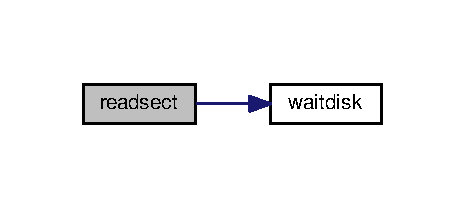
\includegraphics[width=223pt]{d5/dfc/bootmain_8c_ae7ef59ffa082283b72c54e43b7a16351_cgraph}
\end{center}
\end{figure}




Here is the caller graph for this function\+:\nopagebreak
\begin{figure}[H]
\begin{center}
\leavevmode
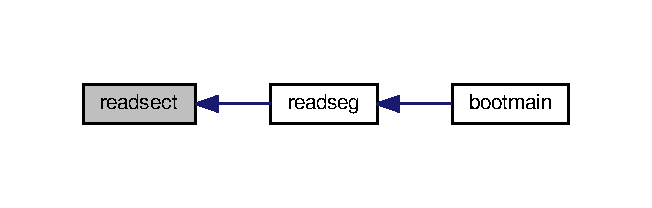
\includegraphics[width=313pt]{d5/dfc/bootmain_8c_ae7ef59ffa082283b72c54e43b7a16351_icgraph}
\end{center}
\end{figure}


\index{bootmain.\+c@{bootmain.\+c}!readseg@{readseg}}
\index{readseg@{readseg}!bootmain.\+c@{bootmain.\+c}}
\subsubsection[{\texorpdfstring{readseg(uchar $\ast$, uint, uint)}{readseg(uchar *, uint, uint)}}]{\setlength{\rightskip}{0pt plus 5cm}void readseg (
\begin{DoxyParamCaption}
\item[{{\bf uchar} $\ast$}]{pa, }
\item[{{\bf uint}}]{count, }
\item[{{\bf uint}}]{offset}
\end{DoxyParamCaption}
)}\hypertarget{bootmain_8c_af8097ce47ae21ccad1b0afd6f48ef62c}{}\label{bootmain_8c_af8097ce47ae21ccad1b0afd6f48ef62c}


Here is the call graph for this function\+:\nopagebreak
\begin{figure}[H]
\begin{center}
\leavevmode
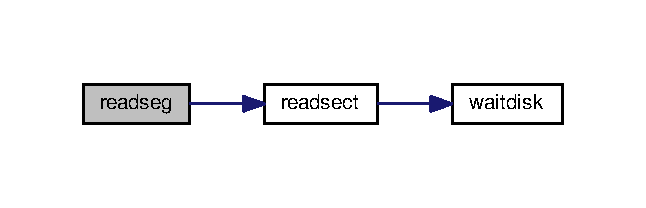
\includegraphics[width=310pt]{d5/dfc/bootmain_8c_af8097ce47ae21ccad1b0afd6f48ef62c_cgraph}
\end{center}
\end{figure}




Here is the caller graph for this function\+:\nopagebreak
\begin{figure}[H]
\begin{center}
\leavevmode
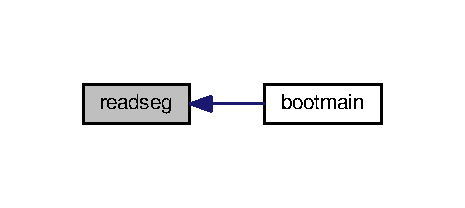
\includegraphics[width=223pt]{d5/dfc/bootmain_8c_af8097ce47ae21ccad1b0afd6f48ef62c_icgraph}
\end{center}
\end{figure}


\index{bootmain.\+c@{bootmain.\+c}!waitdisk@{waitdisk}}
\index{waitdisk@{waitdisk}!bootmain.\+c@{bootmain.\+c}}
\subsubsection[{\texorpdfstring{waitdisk(void)}{waitdisk(void)}}]{\setlength{\rightskip}{0pt plus 5cm}void waitdisk (
\begin{DoxyParamCaption}
\item[{void}]{}
\end{DoxyParamCaption}
)}\hypertarget{bootmain_8c_a63222d4a07c38c198de5bd116a001935}{}\label{bootmain_8c_a63222d4a07c38c198de5bd116a001935}


Here is the caller graph for this function\+:\nopagebreak
\begin{figure}[H]
\begin{center}
\leavevmode
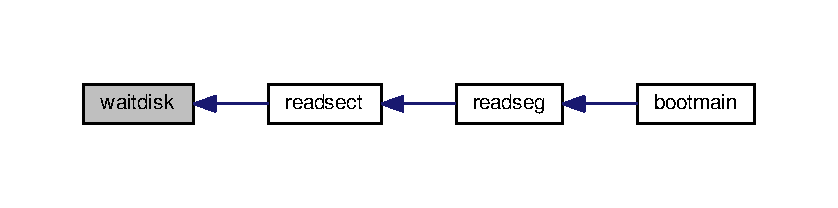
\includegraphics[width=350pt]{d5/dfc/bootmain_8c_a63222d4a07c38c198de5bd116a001935_icgraph}
\end{center}
\end{figure}



\hypertarget{bootmain_8d}{}\section{bootmain.\+d File Reference}
\label{bootmain_8d}\index{bootmain.\+d@{bootmain.\+d}}

\hypertarget{buf_8h}{}\section{buf.\+h File Reference}
\label{buf_8h}\index{buf.\+h@{buf.\+h}}
This graph shows which files directly or indirectly include this file\+:\nopagebreak
\begin{figure}[H]
\begin{center}
\leavevmode
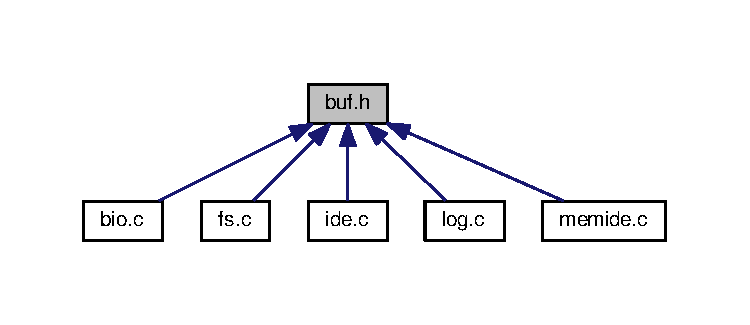
\includegraphics[width=350pt]{db/dec/buf_8h__dep__incl}
\end{center}
\end{figure}
\subsection*{Classes}
\begin{DoxyCompactItemize}
\item 
struct \hyperlink{structbuf}{buf}
\end{DoxyCompactItemize}
\subsection*{Macros}
\begin{DoxyCompactItemize}
\item 
\#define \hyperlink{buf_8h_afab4199c0d27da71061f1c0cd5b51520}{B\+\_\+\+V\+A\+L\+ID}~0x2
\item 
\#define \hyperlink{buf_8h_adc32011df267adb9740bcd0abf0f0663}{B\+\_\+\+D\+I\+R\+TY}~0x4
\end{DoxyCompactItemize}


\subsection{Macro Definition Documentation}
\index{buf.\+h@{buf.\+h}!B\+\_\+\+D\+I\+R\+TY@{B\+\_\+\+D\+I\+R\+TY}}
\index{B\+\_\+\+D\+I\+R\+TY@{B\+\_\+\+D\+I\+R\+TY}!buf.\+h@{buf.\+h}}
\subsubsection[{\texorpdfstring{B\+\_\+\+D\+I\+R\+TY}{B_DIRTY}}]{\setlength{\rightskip}{0pt plus 5cm}\#define B\+\_\+\+D\+I\+R\+TY~0x4}\hypertarget{buf_8h_adc32011df267adb9740bcd0abf0f0663}{}\label{buf_8h_adc32011df267adb9740bcd0abf0f0663}
\index{buf.\+h@{buf.\+h}!B\+\_\+\+V\+A\+L\+ID@{B\+\_\+\+V\+A\+L\+ID}}
\index{B\+\_\+\+V\+A\+L\+ID@{B\+\_\+\+V\+A\+L\+ID}!buf.\+h@{buf.\+h}}
\subsubsection[{\texorpdfstring{B\+\_\+\+V\+A\+L\+ID}{B_VALID}}]{\setlength{\rightskip}{0pt plus 5cm}\#define B\+\_\+\+V\+A\+L\+ID~0x2}\hypertarget{buf_8h_afab4199c0d27da71061f1c0cd5b51520}{}\label{buf_8h_afab4199c0d27da71061f1c0cd5b51520}

\hypertarget{cat_8d}{}\section{cat.\+d File Reference}
\label{cat_8d}\index{cat.\+d@{cat.\+d}}

\hypertarget{console_8c}{}\section{console.\+c File Reference}
\label{console_8c}\index{console.\+c@{console.\+c}}
{\ttfamily \#include \char`\"{}types.\+h\char`\"{}}\\*
{\ttfamily \#include \char`\"{}defs.\+h\char`\"{}}\\*
{\ttfamily \#include \char`\"{}param.\+h\char`\"{}}\\*
{\ttfamily \#include \char`\"{}traps.\+h\char`\"{}}\\*
{\ttfamily \#include \char`\"{}spinlock.\+h\char`\"{}}\\*
{\ttfamily \#include \char`\"{}sleeplock.\+h\char`\"{}}\\*
{\ttfamily \#include \char`\"{}fs.\+h\char`\"{}}\\*
{\ttfamily \#include \char`\"{}file.\+h\char`\"{}}\\*
{\ttfamily \#include \char`\"{}memlayout.\+h\char`\"{}}\\*
{\ttfamily \#include \char`\"{}mmu.\+h\char`\"{}}\\*
{\ttfamily \#include \char`\"{}proc.\+h\char`\"{}}\\*
{\ttfamily \#include \char`\"{}x86.\+h\char`\"{}}\\*
Include dependency graph for console.\+c\+:\nopagebreak
\begin{figure}[H]
\begin{center}
\leavevmode
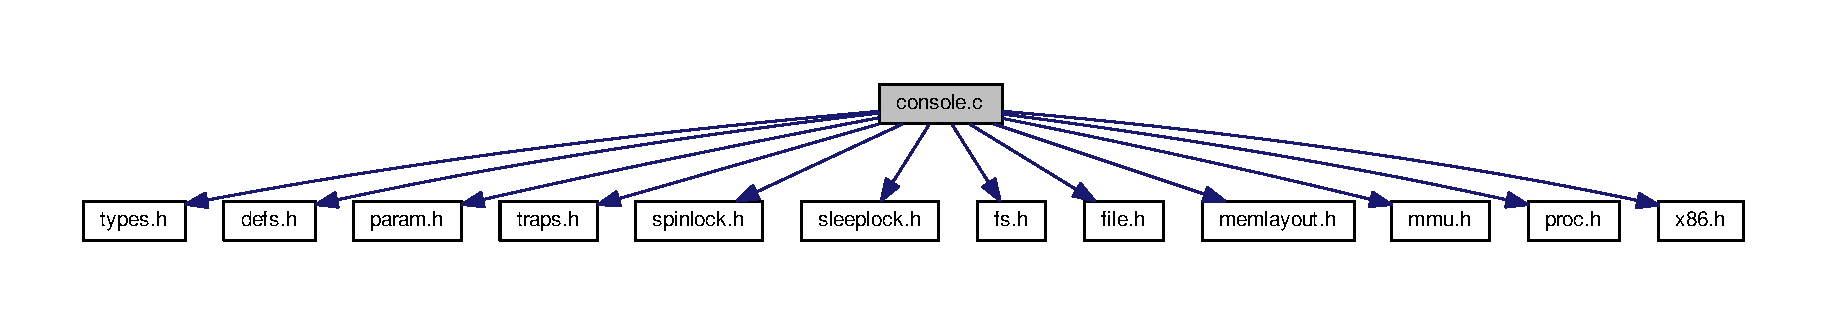
\includegraphics[width=350pt]{df/d7f/console_8c__incl}
\end{center}
\end{figure}
\subsection*{Macros}
\begin{DoxyCompactItemize}
\item 
\#define \hyperlink{console_8c_a629568514359445d2fbda71d70eeb1ce}{B\+A\+C\+K\+S\+P\+A\+CE}~0x100
\item 
\#define \hyperlink{console_8c_a2e3959df0a0c54f50f20d4776b14487f}{C\+R\+T\+P\+O\+RT}~0x3d4
\item 
\#define \hyperlink{console_8c_a5d85434f2a29f6c3048aeac34d0ce41d}{I\+N\+P\+U\+T\+\_\+\+B\+UF}~128
\item 
\#define \hyperlink{console_8c_ac54ae397901fe700628cafadea3c5208}{C}(x)~((x)-\/\textquotesingle{}@\textquotesingle{})
\end{DoxyCompactItemize}
\subsection*{Functions}
\begin{DoxyCompactItemize}
\item 
void \hyperlink{console_8c_a90f0742d846503e4ed1804f1df421ec6}{cprintf} (char $\ast$fmt,...)
\item 
void \hyperlink{console_8c_a95c0aca5d6d7487933984f08b189917a}{panic} (char $\ast$s)
\item 
void \hyperlink{console_8c_aad3d6ca39f23bb6d2686d2967e415193}{consoleintr} (int($\ast$getc)(void))
\item 
int \hyperlink{console_8c_a28ac85a90987662e306ca8efbfe16074}{consoleread} (struct \hyperlink{structinode}{inode} $\ast$ip, char $\ast$dst, int n)
\item 
int \hyperlink{console_8c_a6af7eb39268127d389792cec37785666}{consolewrite} (struct \hyperlink{structinode}{inode} $\ast$ip, char $\ast$\hyperlink{structbuf}{buf}, int n)
\item 
void \hyperlink{console_8c_ab508ff0f4db26fe35cd25fa648f9ee75}{consoleinit} (void)
\end{DoxyCompactItemize}
\subsection*{Variables}
\begin{DoxyCompactItemize}
\item 
\begin{tabbing}
xx\=xx\=xx\=xx\=xx\=xx\=xx\=xx\=xx\=\kill
struct \{\\
\>char \hyperlink{console_8c_aa427837782b05b05204809dfba33c8f5}{buf} \mbox{[}\hyperlink{console_8c_a5d85434f2a29f6c3048aeac34d0ce41d}{INPUT\_BUF}\mbox{]}\\
\>\hyperlink{types_8h_a91ad9478d81a7aaf2593e8d9c3d06a14}{uint} \hyperlink{console_8c_af10fa12dd785c91e29528fbdc50cf9af}{r}\\
\>\hyperlink{types_8h_a91ad9478d81a7aaf2593e8d9c3d06a14}{uint} \hyperlink{console_8c_afdeff54db9a334718662b709641fdfe1}{w}\\
\>\hyperlink{types_8h_a91ad9478d81a7aaf2593e8d9c3d06a14}{uint} \hyperlink{console_8c_ab56fa7c992b725d84916b987c3d532ea}{e}\\
\} \hyperlink{console_8c_a41db130acd332cdb95756628cfb2e48b}{input}\\

\end{tabbing}\end{DoxyCompactItemize}


\subsection{Macro Definition Documentation}
\index{console.\+c@{console.\+c}!B\+A\+C\+K\+S\+P\+A\+CE@{B\+A\+C\+K\+S\+P\+A\+CE}}
\index{B\+A\+C\+K\+S\+P\+A\+CE@{B\+A\+C\+K\+S\+P\+A\+CE}!console.\+c@{console.\+c}}
\subsubsection[{\texorpdfstring{B\+A\+C\+K\+S\+P\+A\+CE}{BACKSPACE}}]{\setlength{\rightskip}{0pt plus 5cm}\#define B\+A\+C\+K\+S\+P\+A\+CE~0x100}\hypertarget{console_8c_a629568514359445d2fbda71d70eeb1ce}{}\label{console_8c_a629568514359445d2fbda71d70eeb1ce}
\index{console.\+c@{console.\+c}!C@{C}}
\index{C@{C}!console.\+c@{console.\+c}}
\subsubsection[{\texorpdfstring{C}{C}}]{\setlength{\rightskip}{0pt plus 5cm}\#define C(
\begin{DoxyParamCaption}
\item[{}]{x}
\end{DoxyParamCaption}
)~((x)-\/\textquotesingle{}@\textquotesingle{})}\hypertarget{console_8c_ac54ae397901fe700628cafadea3c5208}{}\label{console_8c_ac54ae397901fe700628cafadea3c5208}
\index{console.\+c@{console.\+c}!C\+R\+T\+P\+O\+RT@{C\+R\+T\+P\+O\+RT}}
\index{C\+R\+T\+P\+O\+RT@{C\+R\+T\+P\+O\+RT}!console.\+c@{console.\+c}}
\subsubsection[{\texorpdfstring{C\+R\+T\+P\+O\+RT}{CRTPORT}}]{\setlength{\rightskip}{0pt plus 5cm}\#define C\+R\+T\+P\+O\+RT~0x3d4}\hypertarget{console_8c_a2e3959df0a0c54f50f20d4776b14487f}{}\label{console_8c_a2e3959df0a0c54f50f20d4776b14487f}
\index{console.\+c@{console.\+c}!I\+N\+P\+U\+T\+\_\+\+B\+UF@{I\+N\+P\+U\+T\+\_\+\+B\+UF}}
\index{I\+N\+P\+U\+T\+\_\+\+B\+UF@{I\+N\+P\+U\+T\+\_\+\+B\+UF}!console.\+c@{console.\+c}}
\subsubsection[{\texorpdfstring{I\+N\+P\+U\+T\+\_\+\+B\+UF}{INPUT_BUF}}]{\setlength{\rightskip}{0pt plus 5cm}\#define I\+N\+P\+U\+T\+\_\+\+B\+UF~128}\hypertarget{console_8c_a5d85434f2a29f6c3048aeac34d0ce41d}{}\label{console_8c_a5d85434f2a29f6c3048aeac34d0ce41d}


\subsection{Function Documentation}
\index{console.\+c@{console.\+c}!consoleinit@{consoleinit}}
\index{consoleinit@{consoleinit}!console.\+c@{console.\+c}}
\subsubsection[{\texorpdfstring{consoleinit(void)}{consoleinit(void)}}]{\setlength{\rightskip}{0pt plus 5cm}void consoleinit (
\begin{DoxyParamCaption}
\item[{void}]{}
\end{DoxyParamCaption}
)}\hypertarget{console_8c_ab508ff0f4db26fe35cd25fa648f9ee75}{}\label{console_8c_ab508ff0f4db26fe35cd25fa648f9ee75}


Here is the call graph for this function\+:\nopagebreak
\begin{figure}[H]
\begin{center}
\leavevmode
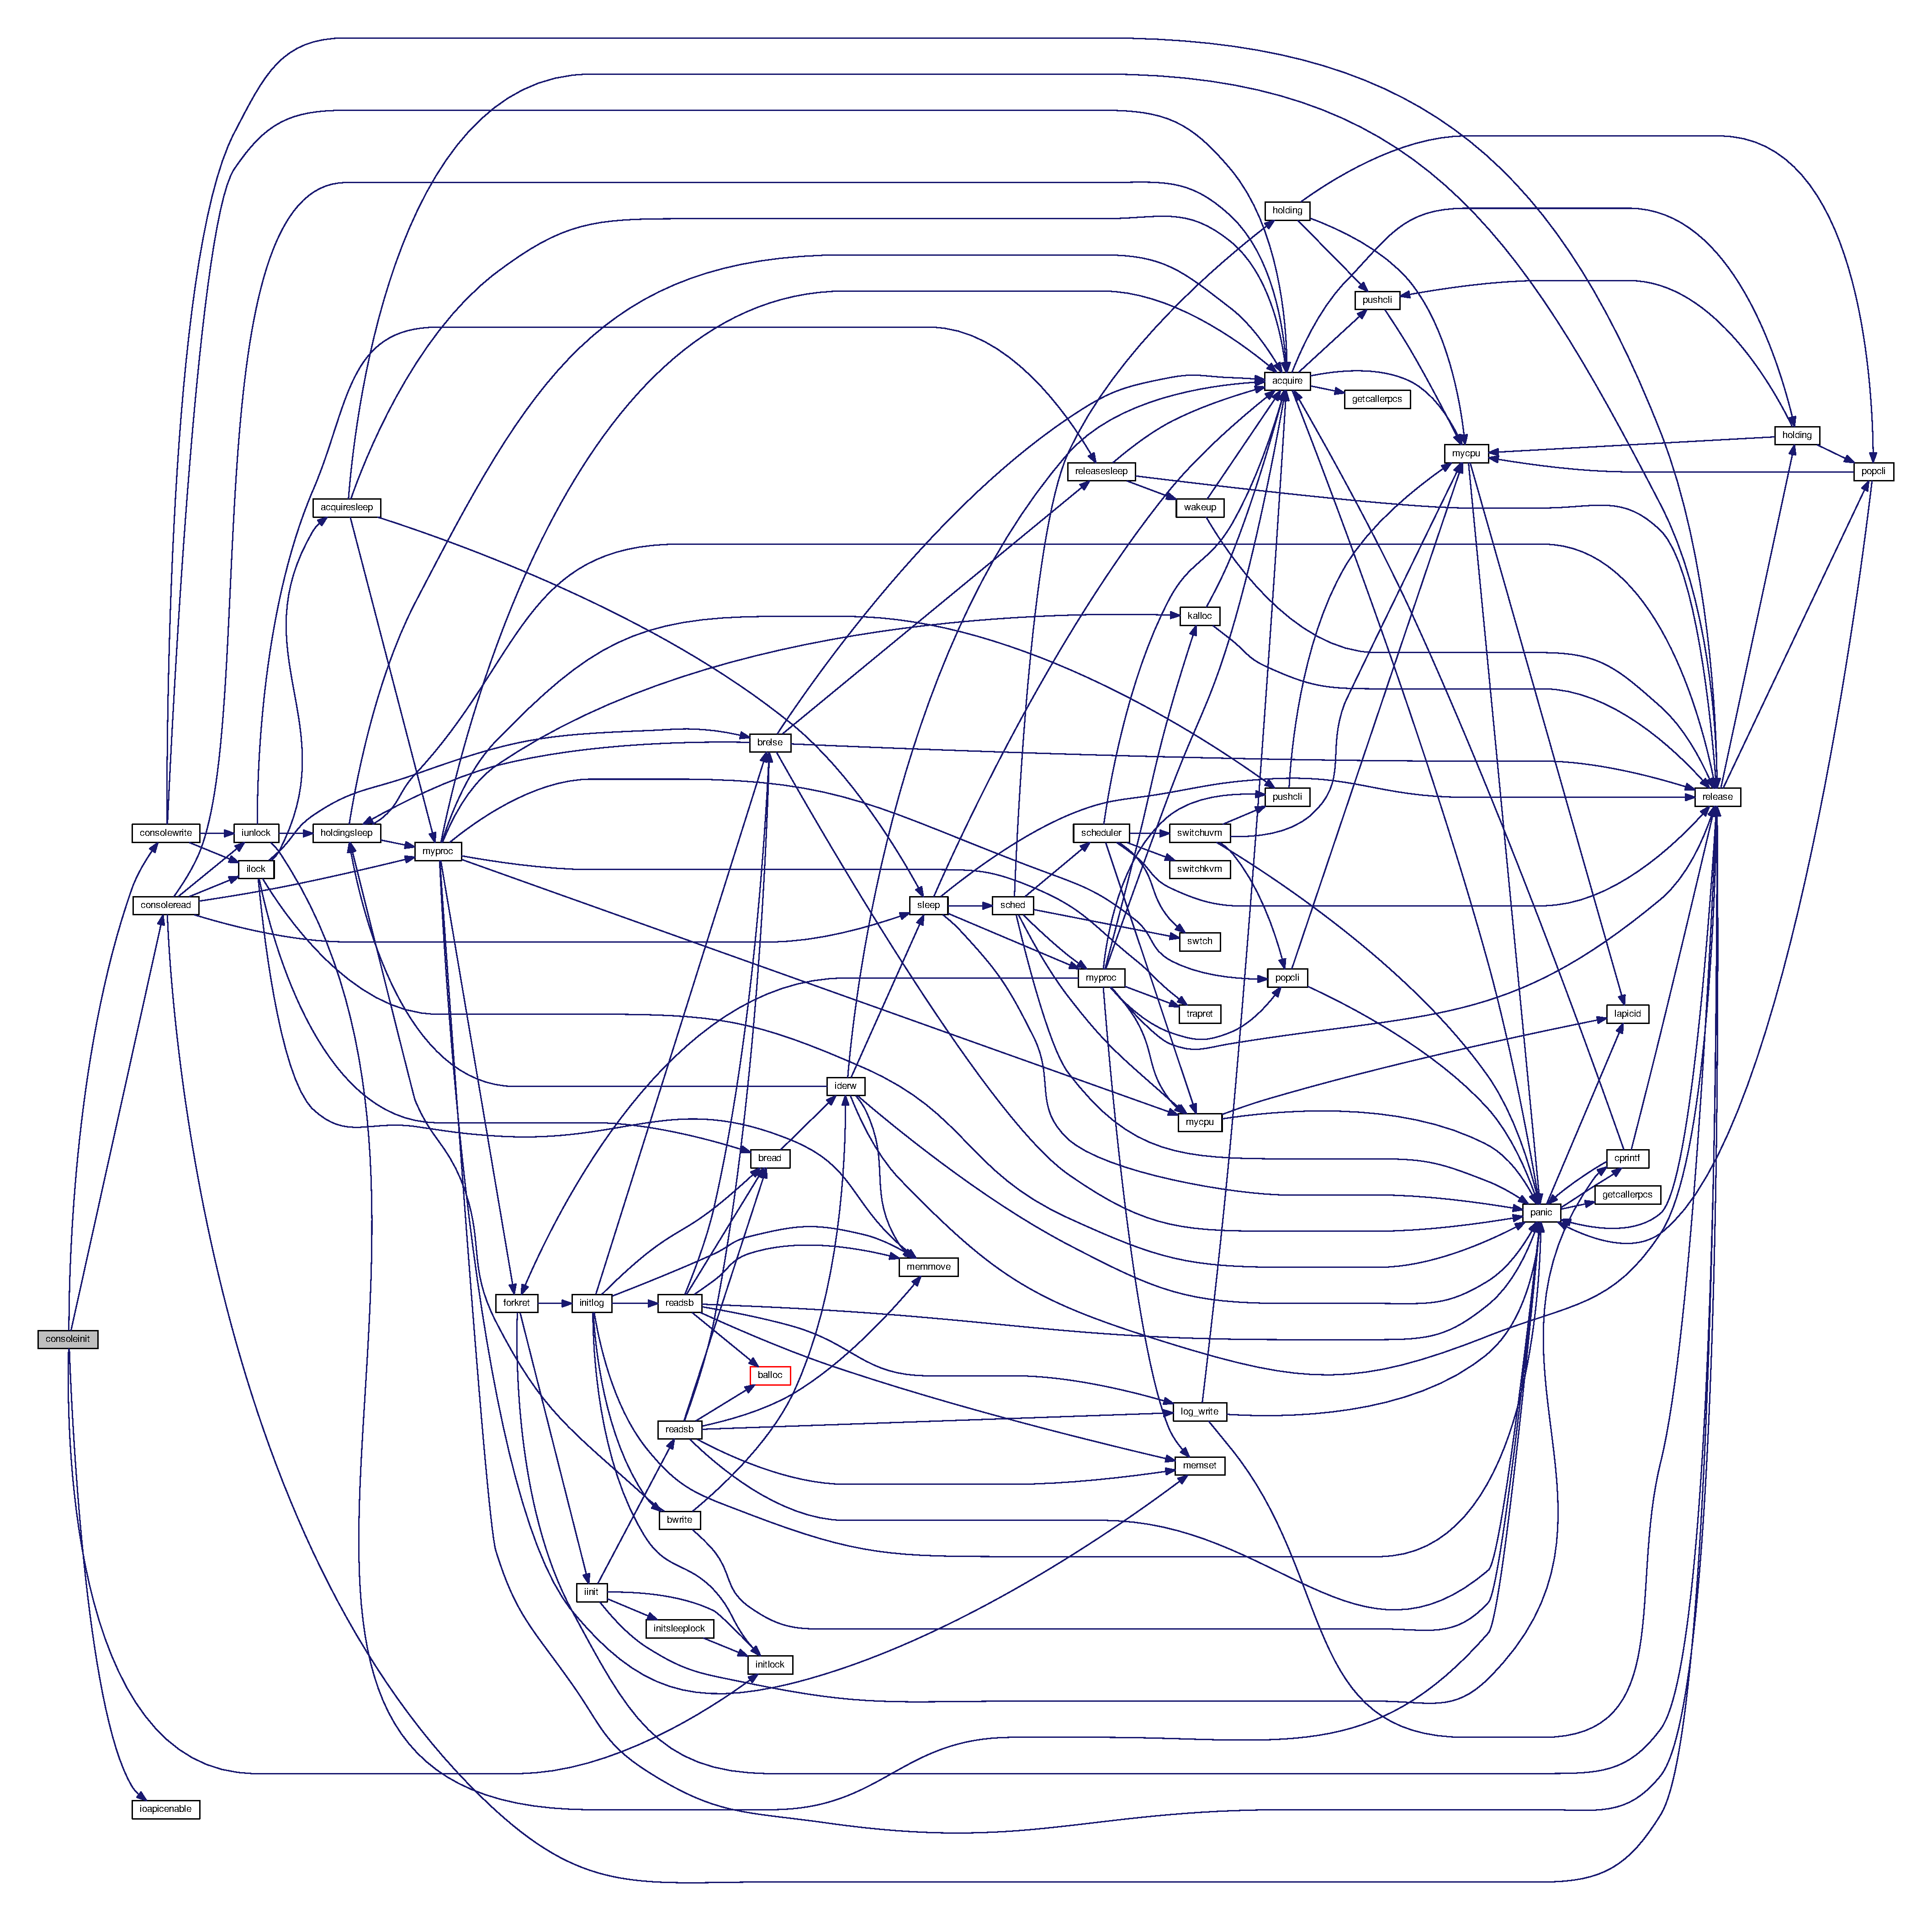
\includegraphics[width=350pt]{d0/d56/console_8c_ab508ff0f4db26fe35cd25fa648f9ee75_cgraph}
\end{center}
\end{figure}


\index{console.\+c@{console.\+c}!consoleintr@{consoleintr}}
\index{consoleintr@{consoleintr}!console.\+c@{console.\+c}}
\subsubsection[{\texorpdfstring{consoleintr(int($\ast$getc)(void))}{consoleintr(int(*getc)(void))}}]{\setlength{\rightskip}{0pt plus 5cm}void consoleintr (
\begin{DoxyParamCaption}
\item[{int($\ast$)(void)}]{getc}
\end{DoxyParamCaption}
)}\hypertarget{console_8c_aad3d6ca39f23bb6d2686d2967e415193}{}\label{console_8c_aad3d6ca39f23bb6d2686d2967e415193}


Here is the call graph for this function\+:\nopagebreak
\begin{figure}[H]
\begin{center}
\leavevmode
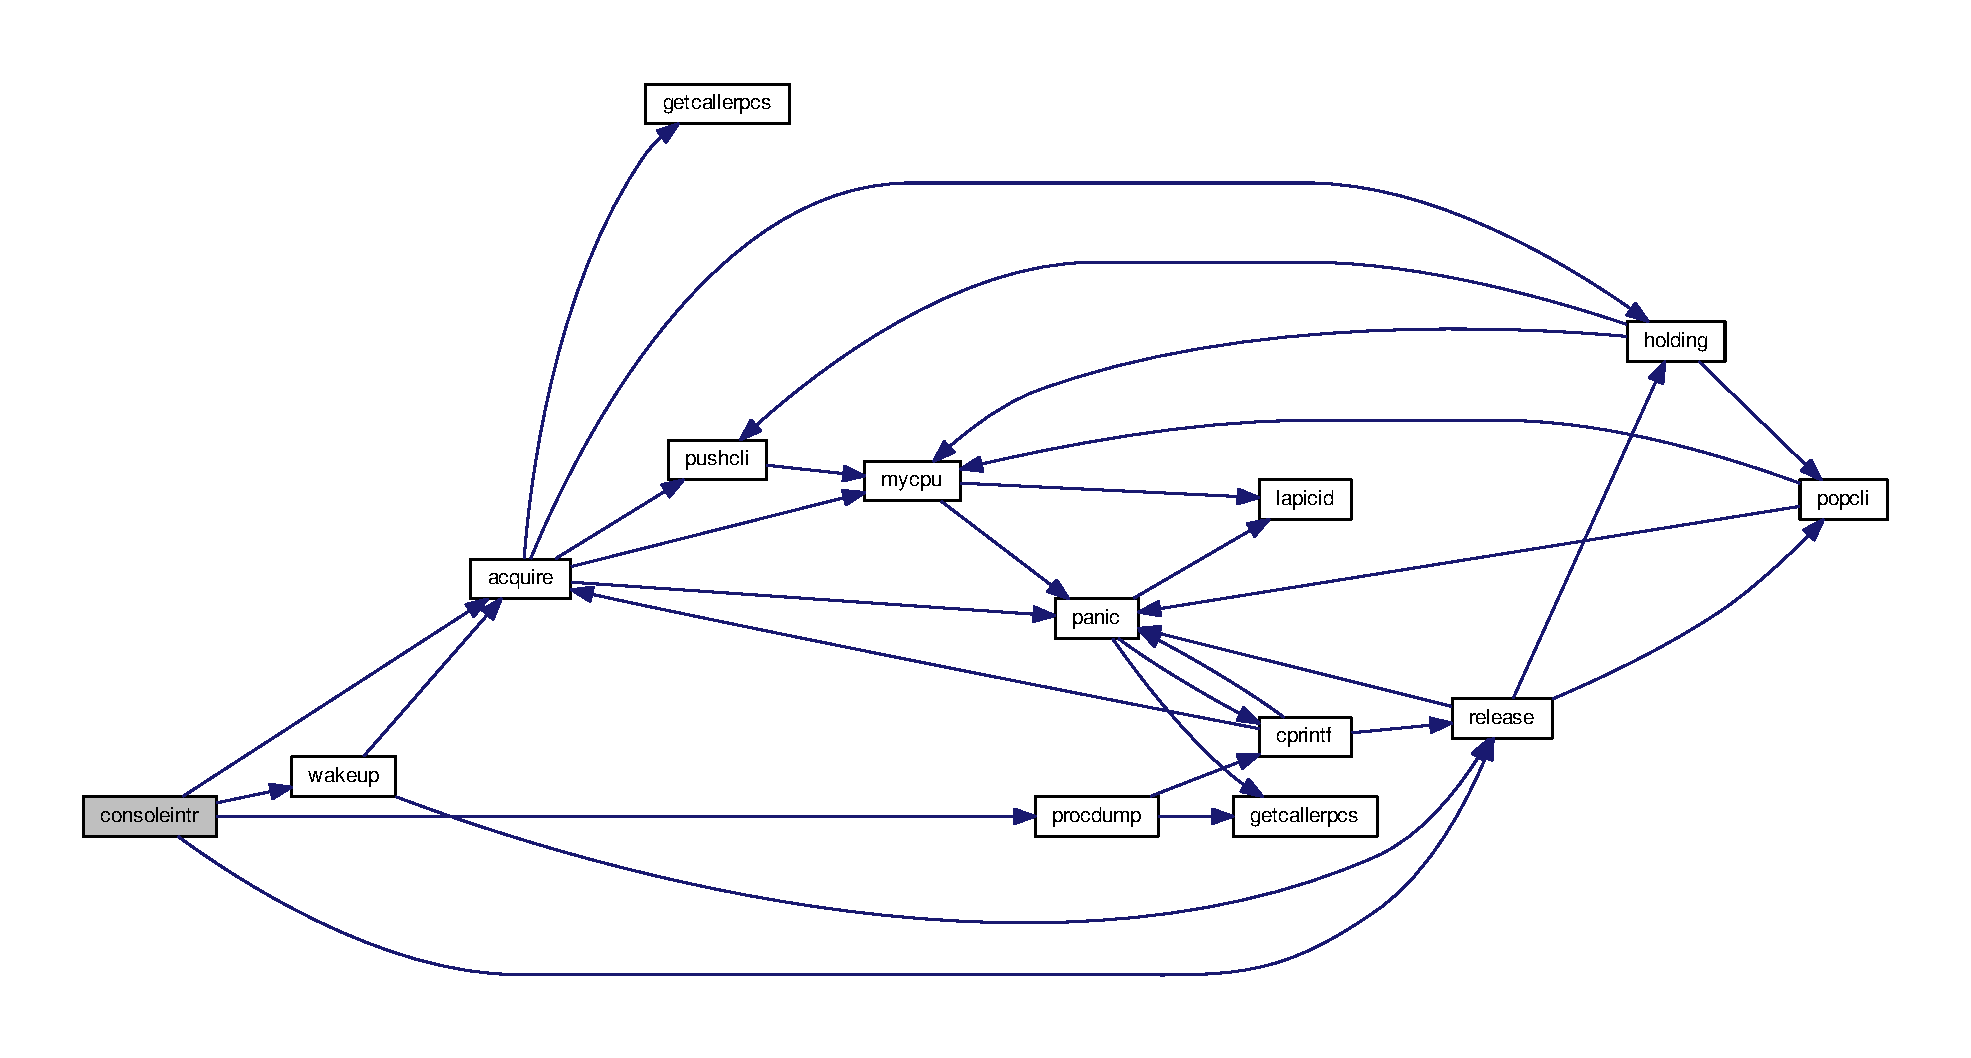
\includegraphics[width=350pt]{d0/d56/console_8c_aad3d6ca39f23bb6d2686d2967e415193_cgraph}
\end{center}
\end{figure}




Here is the caller graph for this function\+:\nopagebreak
\begin{figure}[H]
\begin{center}
\leavevmode
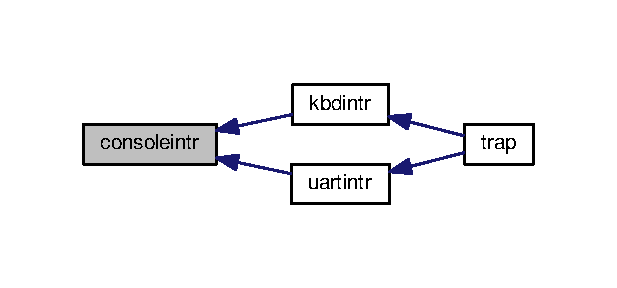
\includegraphics[width=296pt]{d0/d56/console_8c_aad3d6ca39f23bb6d2686d2967e415193_icgraph}
\end{center}
\end{figure}


\index{console.\+c@{console.\+c}!consoleread@{consoleread}}
\index{consoleread@{consoleread}!console.\+c@{console.\+c}}
\subsubsection[{\texorpdfstring{consoleread(struct inode $\ast$ip, char $\ast$dst, int n)}{consoleread(struct inode *ip, char *dst, int n)}}]{\setlength{\rightskip}{0pt plus 5cm}int consoleread (
\begin{DoxyParamCaption}
\item[{struct {\bf inode} $\ast$}]{ip, }
\item[{char $\ast$}]{dst, }
\item[{int}]{n}
\end{DoxyParamCaption}
)}\hypertarget{console_8c_a28ac85a90987662e306ca8efbfe16074}{}\label{console_8c_a28ac85a90987662e306ca8efbfe16074}


Here is the call graph for this function\+:\nopagebreak
\begin{figure}[H]
\begin{center}
\leavevmode
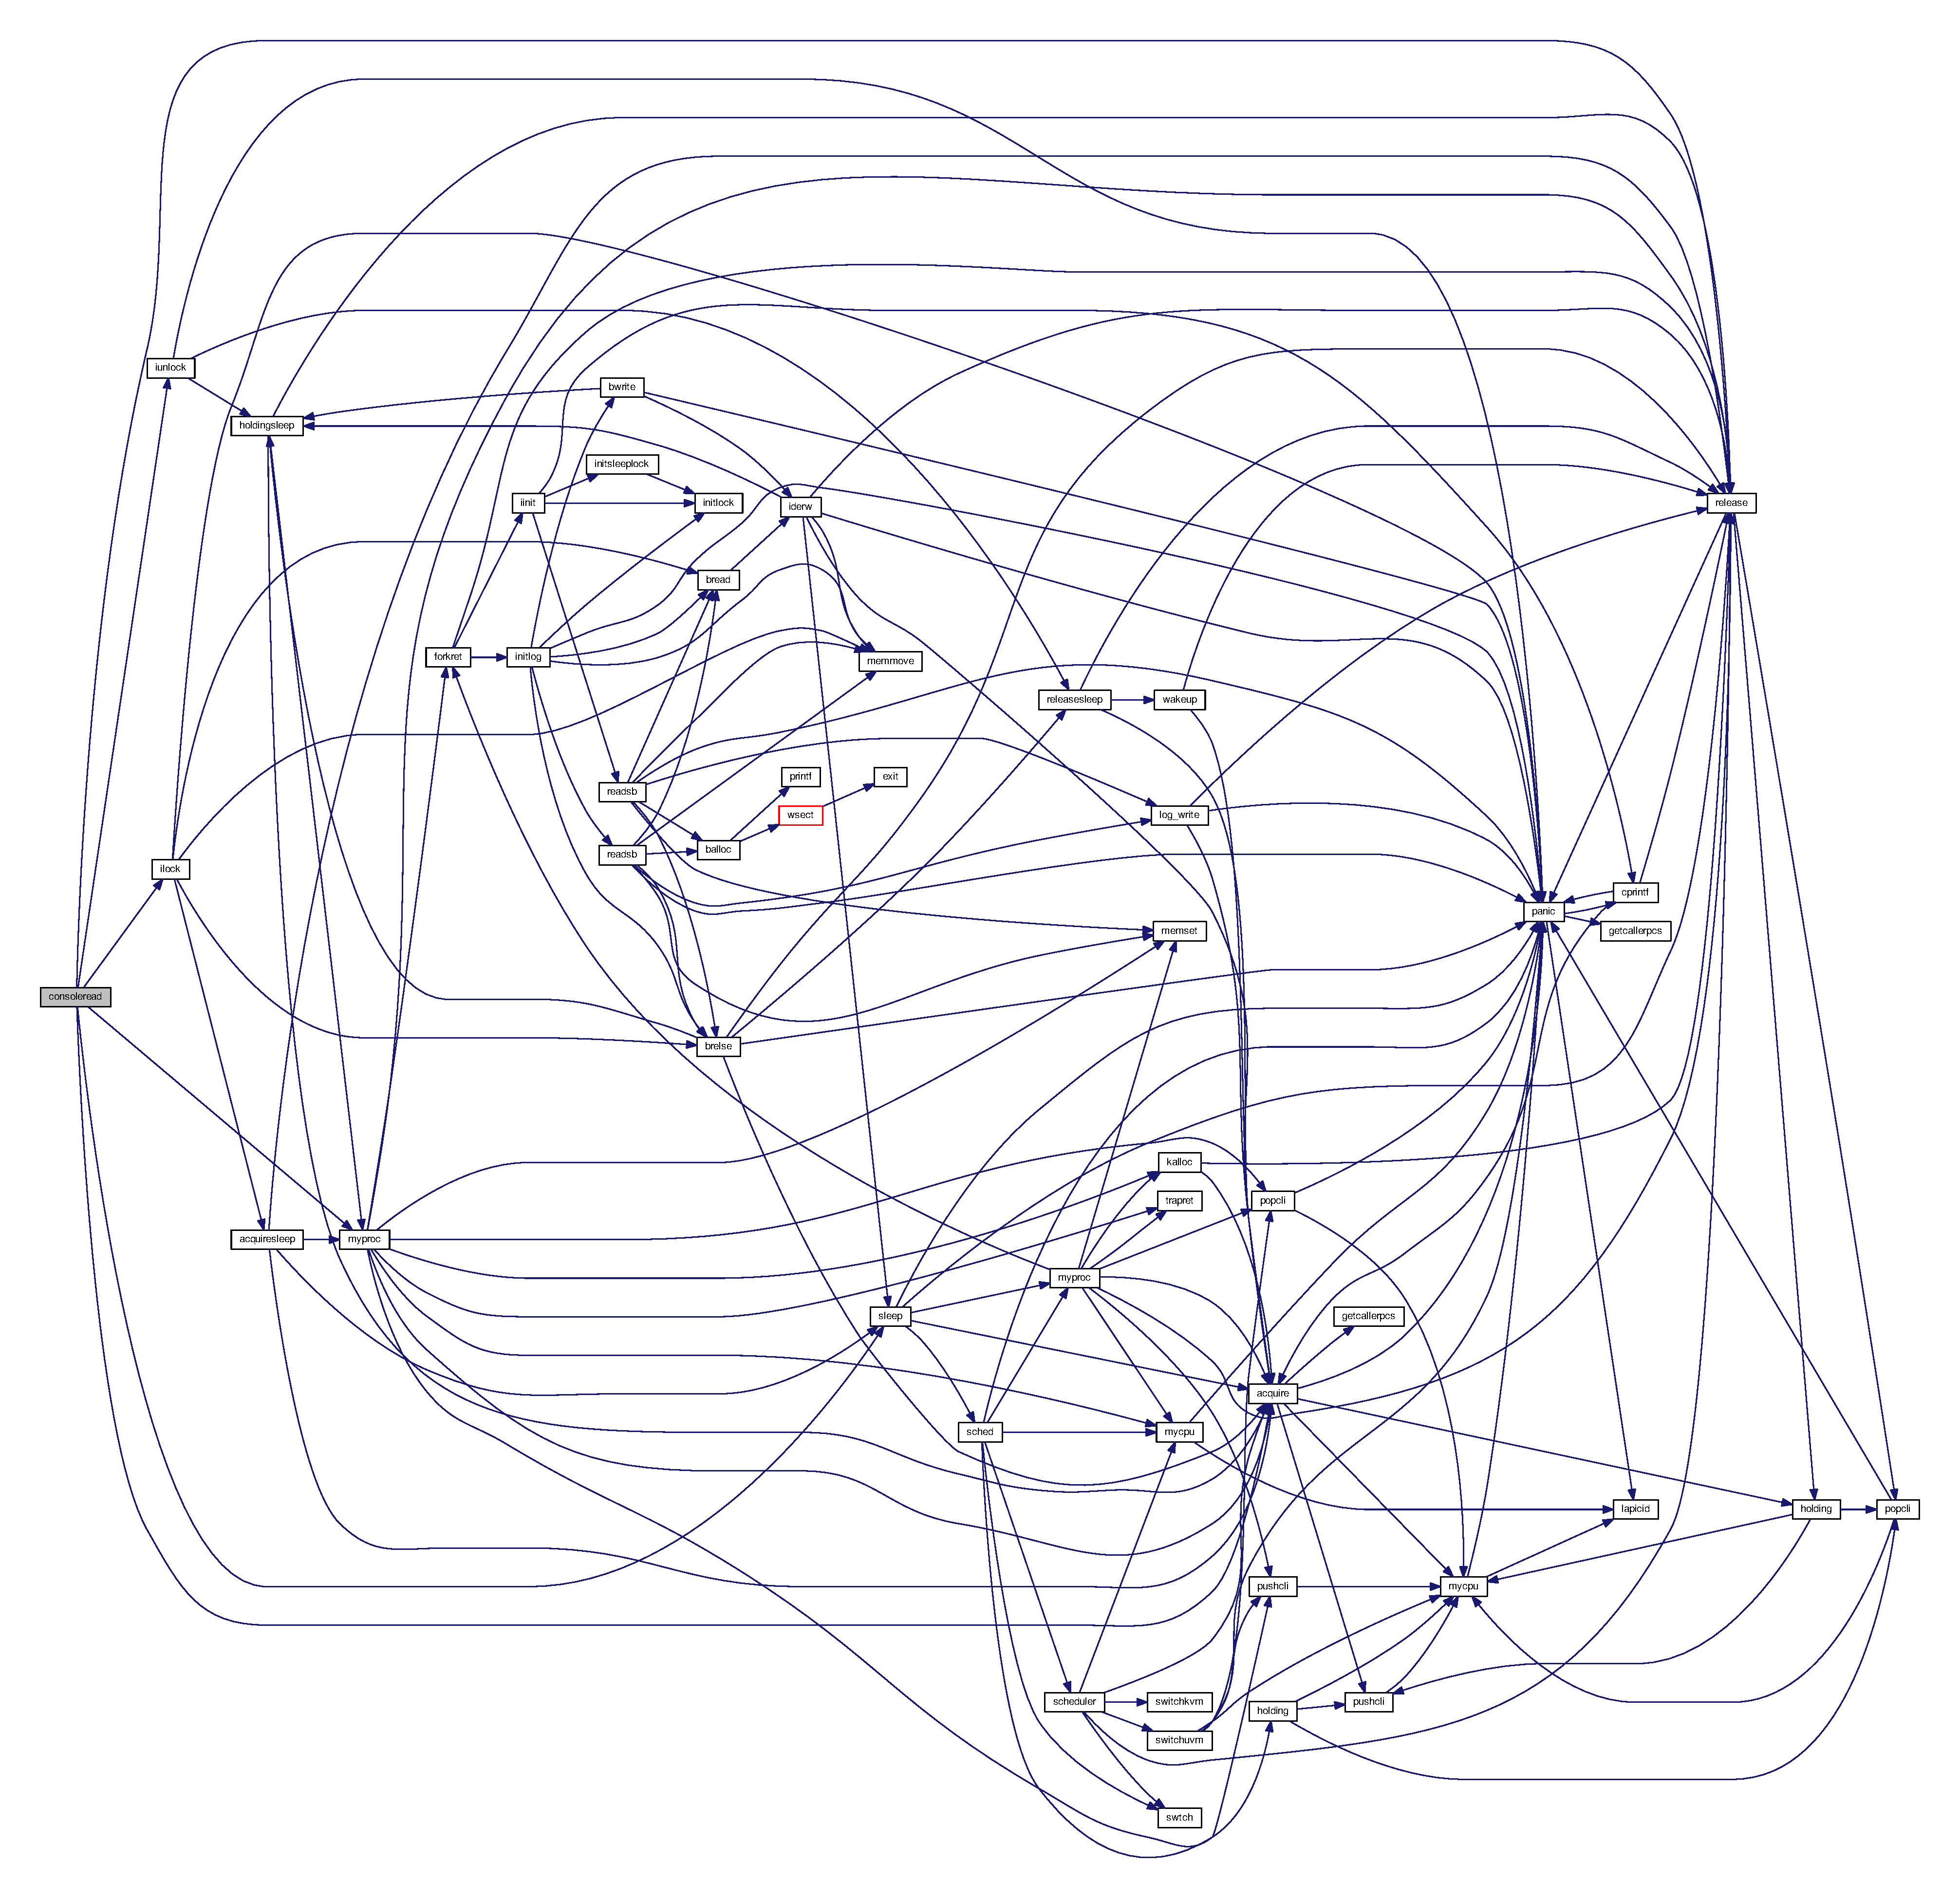
\includegraphics[width=350pt]{d0/d56/console_8c_a28ac85a90987662e306ca8efbfe16074_cgraph}
\end{center}
\end{figure}




Here is the caller graph for this function\+:\nopagebreak
\begin{figure}[H]
\begin{center}
\leavevmode
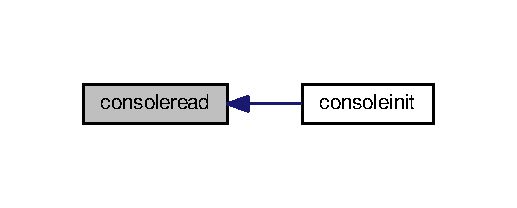
\includegraphics[width=248pt]{d0/d56/console_8c_a28ac85a90987662e306ca8efbfe16074_icgraph}
\end{center}
\end{figure}


\index{console.\+c@{console.\+c}!consolewrite@{consolewrite}}
\index{consolewrite@{consolewrite}!console.\+c@{console.\+c}}
\subsubsection[{\texorpdfstring{consolewrite(struct inode $\ast$ip, char $\ast$buf, int n)}{consolewrite(struct inode *ip, char *buf, int n)}}]{\setlength{\rightskip}{0pt plus 5cm}int consolewrite (
\begin{DoxyParamCaption}
\item[{struct {\bf inode} $\ast$}]{ip, }
\item[{char $\ast$}]{buf, }
\item[{int}]{n}
\end{DoxyParamCaption}
)}\hypertarget{console_8c_a6af7eb39268127d389792cec37785666}{}\label{console_8c_a6af7eb39268127d389792cec37785666}


Here is the call graph for this function\+:\nopagebreak
\begin{figure}[H]
\begin{center}
\leavevmode
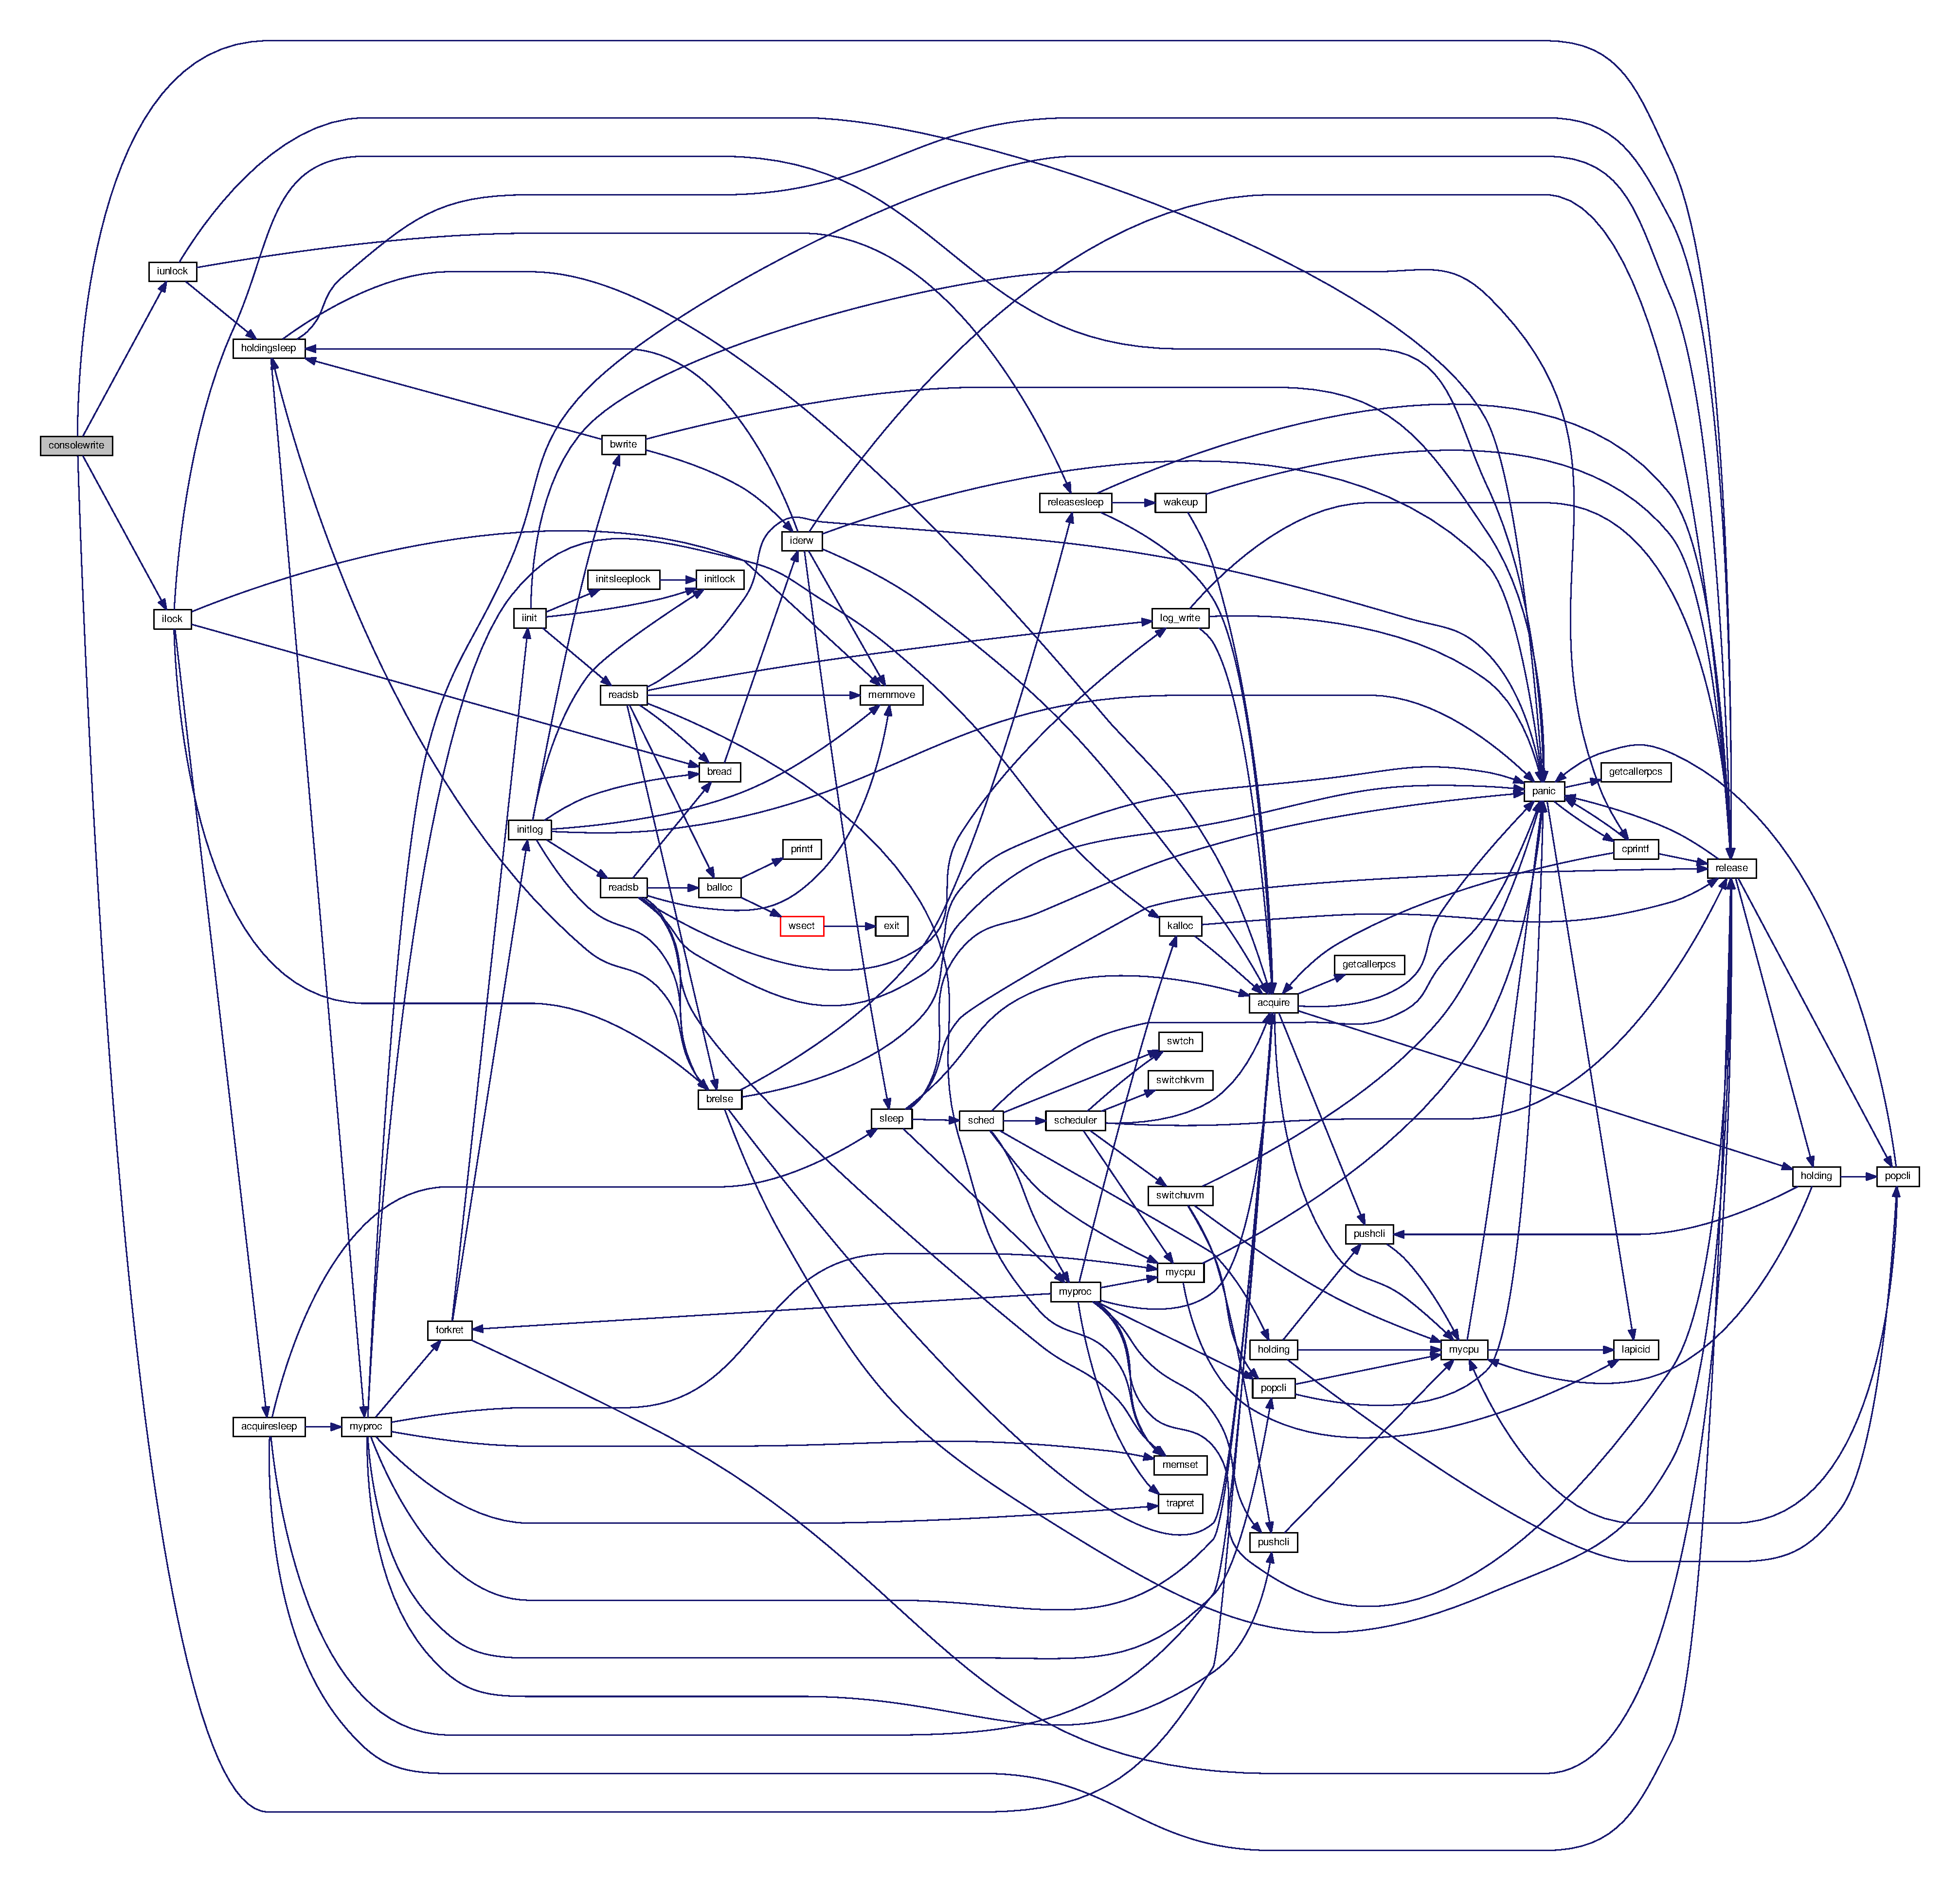
\includegraphics[width=350pt]{d0/d56/console_8c_a6af7eb39268127d389792cec37785666_cgraph}
\end{center}
\end{figure}




Here is the caller graph for this function\+:\nopagebreak
\begin{figure}[H]
\begin{center}
\leavevmode
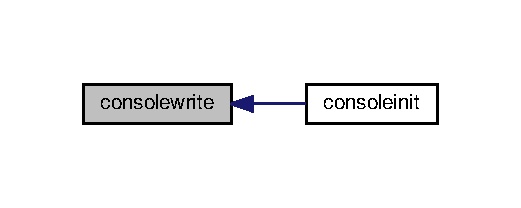
\includegraphics[width=250pt]{d0/d56/console_8c_a6af7eb39268127d389792cec37785666_icgraph}
\end{center}
\end{figure}


\index{console.\+c@{console.\+c}!cprintf@{cprintf}}
\index{cprintf@{cprintf}!console.\+c@{console.\+c}}
\subsubsection[{\texorpdfstring{cprintf(char $\ast$fmt,...)}{cprintf(char *fmt,...)}}]{\setlength{\rightskip}{0pt plus 5cm}void cprintf (
\begin{DoxyParamCaption}
\item[{char $\ast$}]{fmt, }
\item[{}]{...}
\end{DoxyParamCaption}
)}\hypertarget{console_8c_a90f0742d846503e4ed1804f1df421ec6}{}\label{console_8c_a90f0742d846503e4ed1804f1df421ec6}


Here is the call graph for this function\+:\nopagebreak
\begin{figure}[H]
\begin{center}
\leavevmode
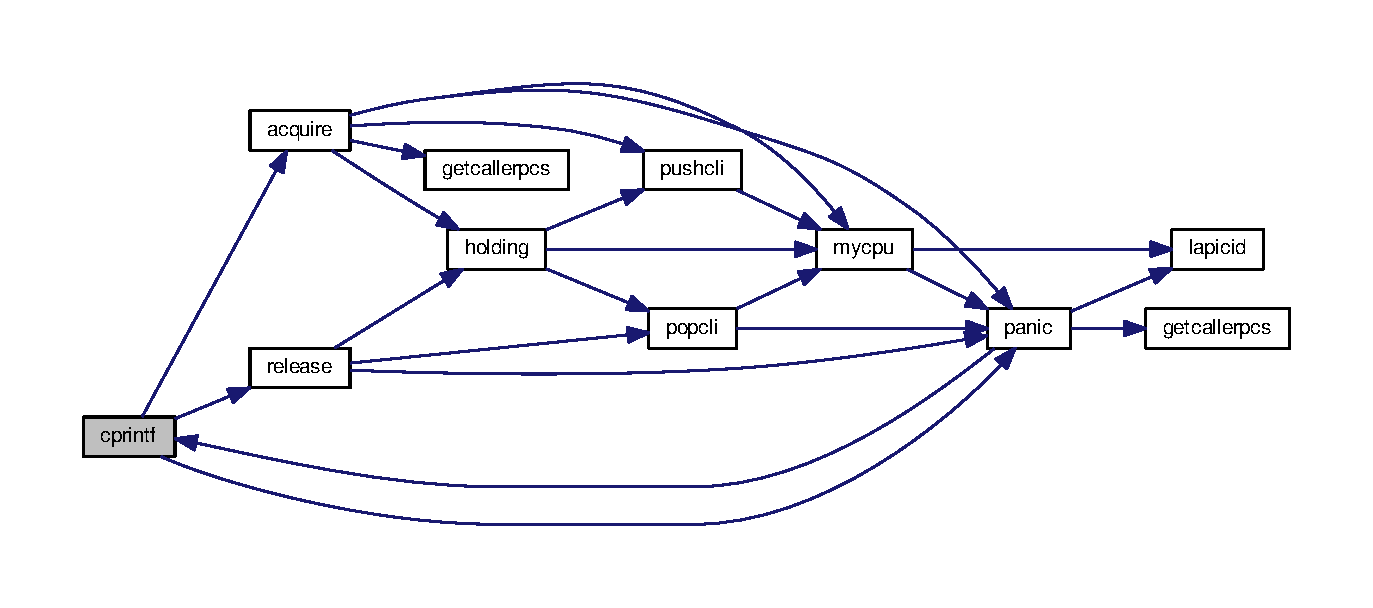
\includegraphics[width=350pt]{d0/d56/console_8c_a90f0742d846503e4ed1804f1df421ec6_cgraph}
\end{center}
\end{figure}




Here is the caller graph for this function\+:\nopagebreak
\begin{figure}[H]
\begin{center}
\leavevmode
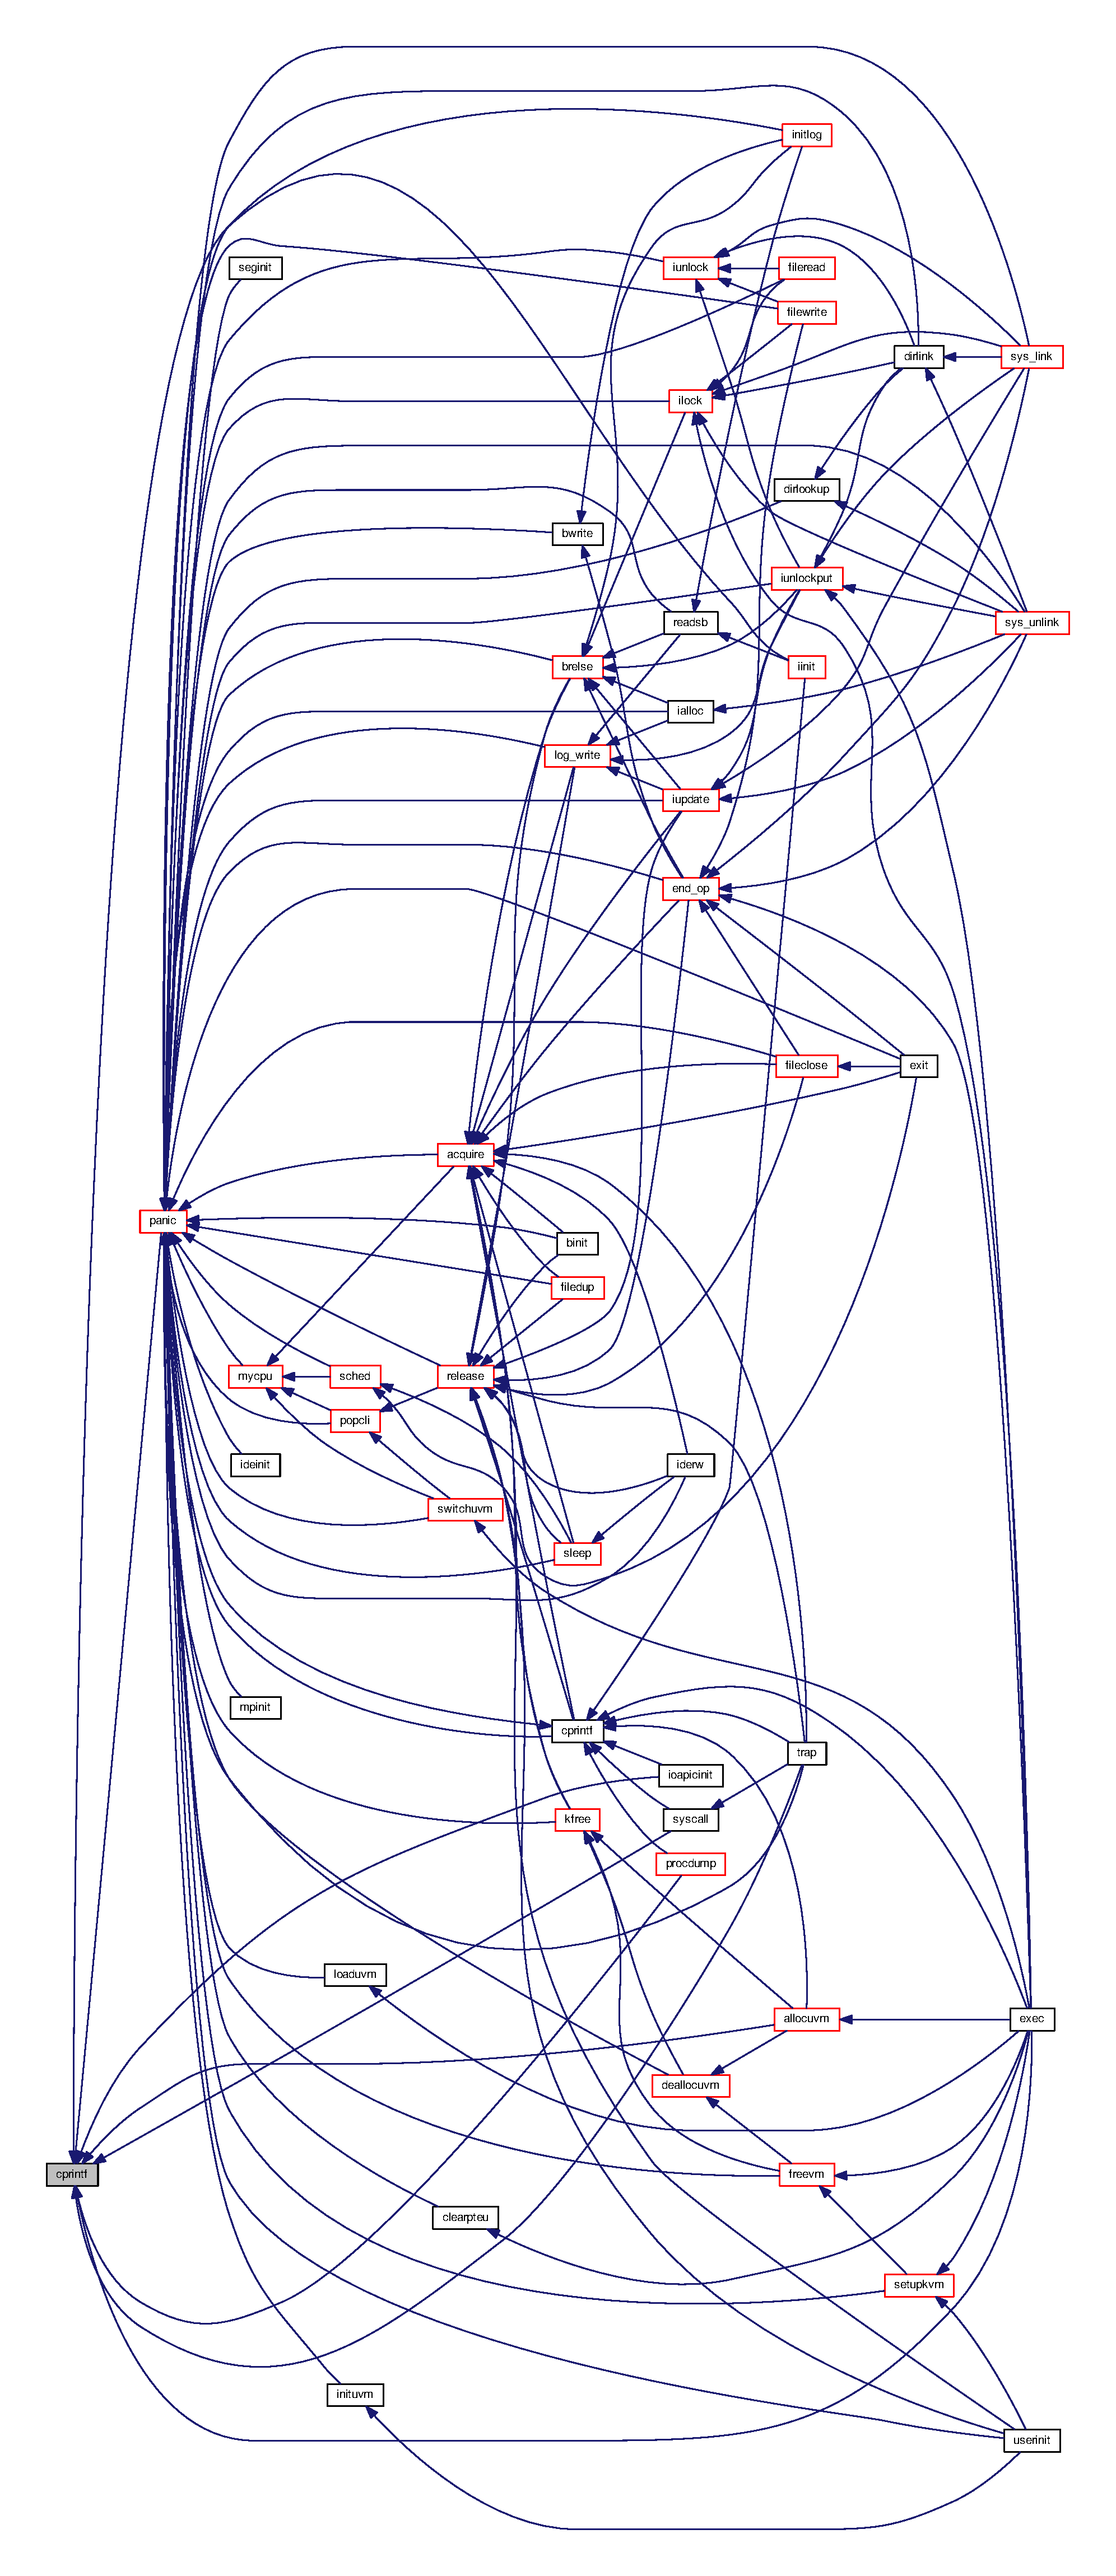
\includegraphics[height=550pt]{d0/d56/console_8c_a90f0742d846503e4ed1804f1df421ec6_icgraph}
\end{center}
\end{figure}


\index{console.\+c@{console.\+c}!panic@{panic}}
\index{panic@{panic}!console.\+c@{console.\+c}}
\subsubsection[{\texorpdfstring{panic(char $\ast$s)}{panic(char *s)}}]{\setlength{\rightskip}{0pt plus 5cm}void panic (
\begin{DoxyParamCaption}
\item[{char $\ast$}]{s}
\end{DoxyParamCaption}
)}\hypertarget{console_8c_a95c0aca5d6d7487933984f08b189917a}{}\label{console_8c_a95c0aca5d6d7487933984f08b189917a}


Here is the call graph for this function\+:\nopagebreak
\begin{figure}[H]
\begin{center}
\leavevmode
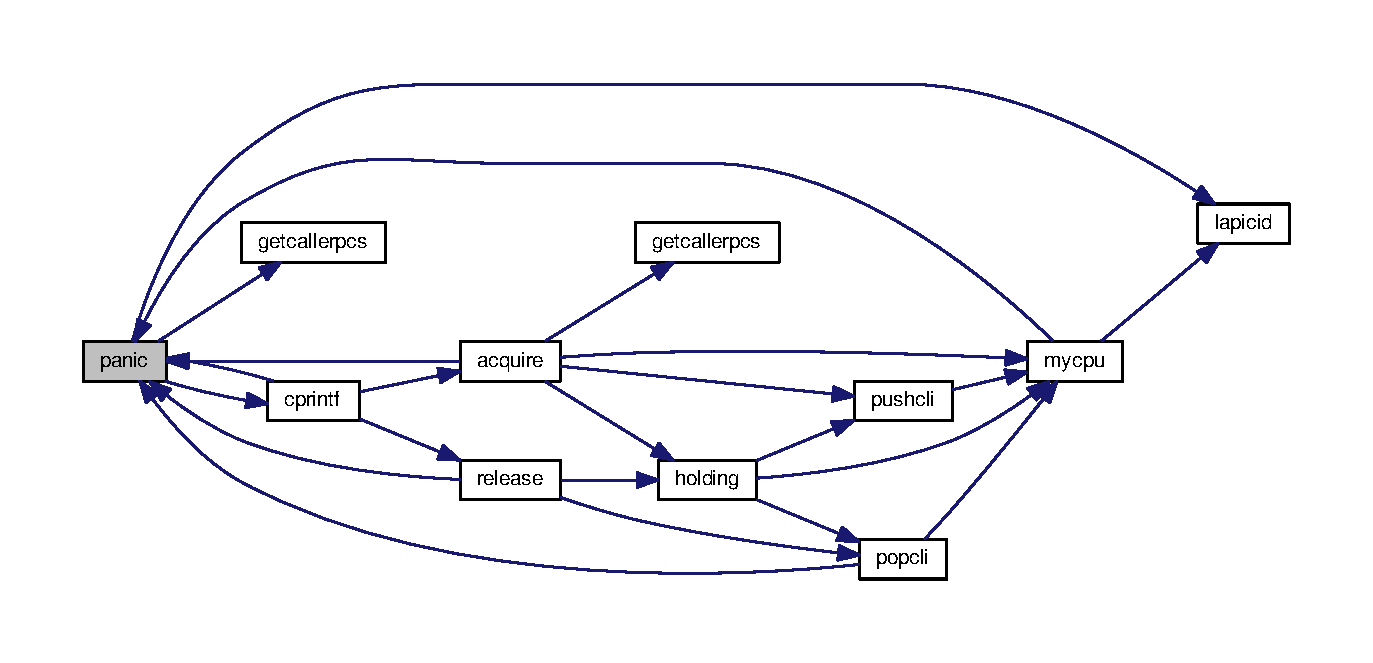
\includegraphics[width=350pt]{d0/d56/console_8c_a95c0aca5d6d7487933984f08b189917a_cgraph}
\end{center}
\end{figure}




Here is the caller graph for this function\+:\nopagebreak
\begin{figure}[H]
\begin{center}
\leavevmode
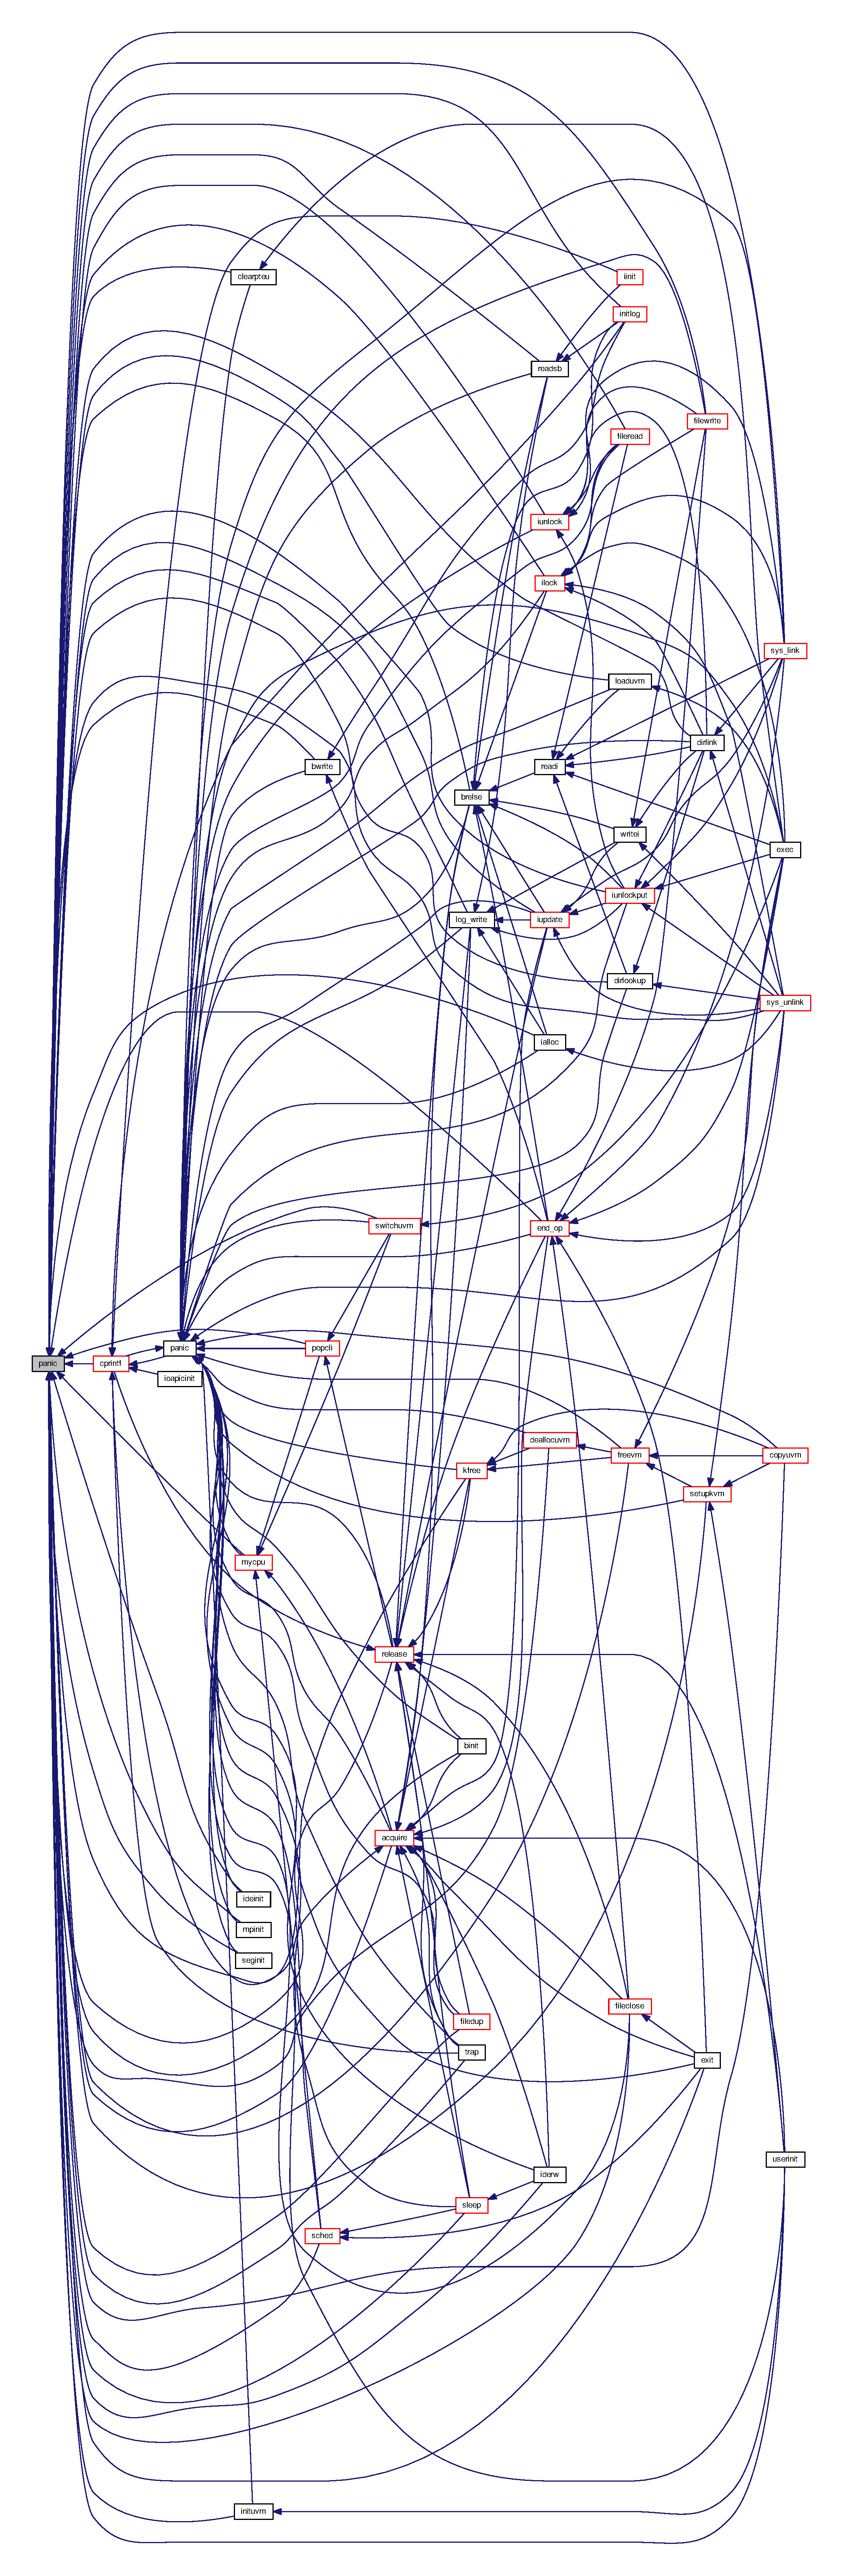
\includegraphics[height=550pt]{d0/d56/console_8c_a95c0aca5d6d7487933984f08b189917a_icgraph}
\end{center}
\end{figure}




\subsection{Variable Documentation}
\index{console.\+c@{console.\+c}!buf@{buf}}
\index{buf@{buf}!console.\+c@{console.\+c}}
\subsubsection[{\texorpdfstring{buf}{buf}}]{\setlength{\rightskip}{0pt plus 5cm}char {\bf buf}\mbox{[}{\bf I\+N\+P\+U\+T\+\_\+\+B\+UF}\mbox{]}}\hypertarget{console_8c_aa427837782b05b05204809dfba33c8f5}{}\label{console_8c_aa427837782b05b05204809dfba33c8f5}
\index{console.\+c@{console.\+c}!e@{e}}
\index{e@{e}!console.\+c@{console.\+c}}
\subsubsection[{\texorpdfstring{e}{e}}]{\setlength{\rightskip}{0pt plus 5cm}{\bf uint} e}\hypertarget{console_8c_ab56fa7c992b725d84916b987c3d532ea}{}\label{console_8c_ab56fa7c992b725d84916b987c3d532ea}
\index{console.\+c@{console.\+c}!input@{input}}
\index{input@{input}!console.\+c@{console.\+c}}
\subsubsection[{\texorpdfstring{input}{input}}]{\setlength{\rightskip}{0pt plus 5cm}struct \{ ... \}   input}\hypertarget{console_8c_a41db130acd332cdb95756628cfb2e48b}{}\label{console_8c_a41db130acd332cdb95756628cfb2e48b}
\index{console.\+c@{console.\+c}!lock@{lock}}
\index{lock@{lock}!console.\+c@{console.\+c}}
\subsubsection[{\texorpdfstring{lock}{lock}}]{\setlength{\rightskip}{0pt plus 5cm}struct {\bf spinlock} lock}\hypertarget{console_8c_ab28e82cd5dda7d960095706a3ea20572}{}\label{console_8c_ab28e82cd5dda7d960095706a3ea20572}
\index{console.\+c@{console.\+c}!locking@{locking}}
\index{locking@{locking}!console.\+c@{console.\+c}}
\subsubsection[{\texorpdfstring{locking}{locking}}]{\setlength{\rightskip}{0pt plus 5cm}int locking}\hypertarget{console_8c_ae51110da3bc13ef49e32d1e2cda5d55c}{}\label{console_8c_ae51110da3bc13ef49e32d1e2cda5d55c}
\index{console.\+c@{console.\+c}!r@{r}}
\index{r@{r}!console.\+c@{console.\+c}}
\subsubsection[{\texorpdfstring{r}{r}}]{\setlength{\rightskip}{0pt plus 5cm}{\bf uint} r}\hypertarget{console_8c_af10fa12dd785c91e29528fbdc50cf9af}{}\label{console_8c_af10fa12dd785c91e29528fbdc50cf9af}
\index{console.\+c@{console.\+c}!w@{w}}
\index{w@{w}!console.\+c@{console.\+c}}
\subsubsection[{\texorpdfstring{w}{w}}]{\setlength{\rightskip}{0pt plus 5cm}{\bf uint} w}\hypertarget{console_8c_afdeff54db9a334718662b709641fdfe1}{}\label{console_8c_afdeff54db9a334718662b709641fdfe1}

\hypertarget{console_8d}{}\section{console.\+d File Reference}
\label{console_8d}\index{console.\+d@{console.\+d}}

\hypertarget{date_8h}{}\section{date.\+h File Reference}
\label{date_8h}\index{date.\+h@{date.\+h}}
This graph shows which files directly or indirectly include this file\+:\nopagebreak
\begin{figure}[H]
\begin{center}
\leavevmode
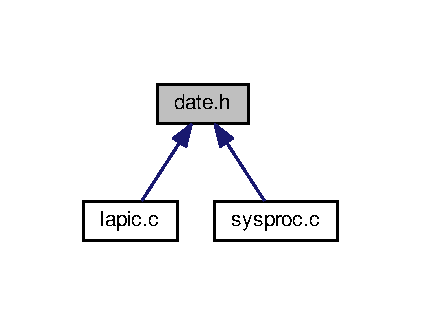
\includegraphics[width=202pt]{d1/dfd/date_8h__dep__incl}
\end{center}
\end{figure}
\subsection*{Classes}
\begin{DoxyCompactItemize}
\item 
struct \hyperlink{structrtcdate}{rtcdate}
\end{DoxyCompactItemize}

\hypertarget{defs_8h}{}\section{defs.\+h File Reference}
\label{defs_8h}\index{defs.\+h@{defs.\+h}}
This graph shows which files directly or indirectly include this file\+:\nopagebreak
\begin{figure}[H]
\begin{center}
\leavevmode
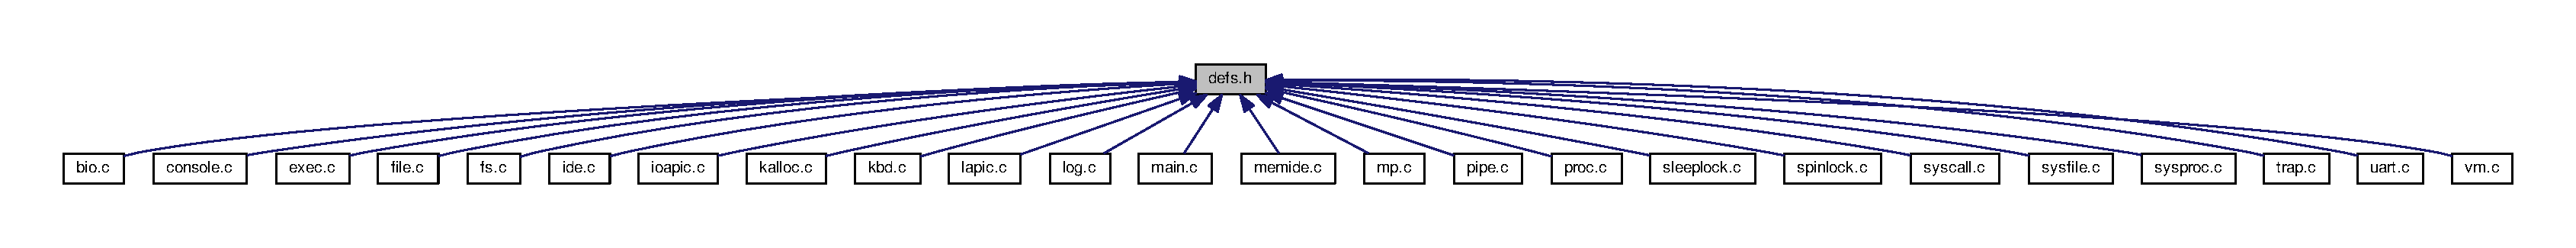
\includegraphics[width=350pt]{d2/d3c/defs_8h__dep__incl}
\end{center}
\end{figure}
\subsection*{Macros}
\begin{DoxyCompactItemize}
\item 
\#define \hyperlink{defs_8h_afacd331296c10f360da7640e0d68429f}{N\+E\+L\+EM}(x)~(sizeof(x)/sizeof((x)\mbox{[}0\mbox{]}))
\end{DoxyCompactItemize}
\subsection*{Functions}
\begin{DoxyCompactItemize}
\item 
void \hyperlink{defs_8h_a53cca0ddc98c5f1de37124eca2575a59}{binit} (void)
\item 
struct \hyperlink{structbuf}{buf} $\ast$ \hyperlink{defs_8h_a90c72cf2140fdf1612484117327220af}{bread} (\hyperlink{types_8h_a91ad9478d81a7aaf2593e8d9c3d06a14}{uint}, \hyperlink{types_8h_a91ad9478d81a7aaf2593e8d9c3d06a14}{uint})
\item 
void \hyperlink{defs_8h_aa31ec2f79e0456737a9680270bc1841b}{brelse} (struct \hyperlink{structbuf}{buf} $\ast$)
\item 
void \hyperlink{defs_8h_a1bfd775f14ad3dfee354ee3897ecd28d}{bwrite} (struct \hyperlink{structbuf}{buf} $\ast$)
\item 
void \hyperlink{defs_8h_ab508ff0f4db26fe35cd25fa648f9ee75}{consoleinit} (void)
\item 
void \hyperlink{defs_8h_abeb2bc020e7332bcde1d7beab08582d3}{cprintf} (char $\ast$,...)
\item 
void \hyperlink{defs_8h_a9ec968a6fc407075634fe0e82a9c6862}{consoleintr} (int($\ast$)(void))
\item 
void \hyperlink{defs_8h_a45323e3f295a0d9b90929cc30a24e2aa}{panic} (char $\ast$) \hyperlink{main_8c_a08f0b7c20a38fda2383d4f70bb78dc3e}{\+\_\+\+\_\+attribute\+\_\+\+\_\+}((noreturn))
\item 
int \hyperlink{defs_8h_aa7b4aae4a12acd187e23396214aeca47}{exec} (char $\ast$, char $\ast$$\ast$)
\item 
struct \hyperlink{structfile}{file} $\ast$ \hyperlink{defs_8h_a69d3d2dd94efa1f1ff8d0143f4d9b786}{filealloc} (void)
\item 
void \hyperlink{defs_8h_ac865ee0b2d70f753d61d1fefef9de0f6}{fileclose} (struct \hyperlink{structfile}{file} $\ast$)
\item 
struct \hyperlink{structfile}{file} $\ast$ \hyperlink{defs_8h_a1063546fe0d5f45fe1a38a9b4f6b5783}{filedup} (struct \hyperlink{structfile}{file} $\ast$)
\item 
void \hyperlink{defs_8h_a66bb5a4b304ea0f851dd999fc8195fa4}{fileinit} (void)
\item 
int \hyperlink{defs_8h_a6bd1db179155944c9d1fbc89d8b7b162}{fileread} (struct \hyperlink{structfile}{file} $\ast$, char $\ast$, int n)
\item 
int \hyperlink{defs_8h_ac4979f97957194db01001985b1bfa84e}{filestat} (struct \hyperlink{structfile}{file} $\ast$, struct \hyperlink{structstat}{stat} $\ast$)
\item 
int \hyperlink{defs_8h_a90e8980df48fa900fc33de53448a2e18}{filewrite} (struct \hyperlink{structfile}{file} $\ast$, char $\ast$, int n)
\item 
void \hyperlink{defs_8h_aff0080b2133027be2e525ca088b40e78}{readsb} (int dev, struct \hyperlink{structsuperblock}{superblock} $\ast$\hyperlink{mkfs_8c_a0248d0bac625de5a1415f2f8c91f3343}{sb})
\item 
int \hyperlink{defs_8h_ae4ccea0aa02557162963e597737f665a}{dirlink} (struct \hyperlink{structinode}{inode} $\ast$, char $\ast$, \hyperlink{types_8h_a91ad9478d81a7aaf2593e8d9c3d06a14}{uint})
\item 
struct \hyperlink{structinode}{inode} $\ast$ \hyperlink{defs_8h_a91ded9e61402d5e0d9f16b2a8cbff5c3}{dirlookup} (struct \hyperlink{structinode}{inode} $\ast$, char $\ast$, \hyperlink{types_8h_a91ad9478d81a7aaf2593e8d9c3d06a14}{uint} $\ast$)
\item 
struct \hyperlink{structinode}{inode} $\ast$ \hyperlink{defs_8h_ab4d7f391ca5219199e1b7502ac12ea85}{ialloc} (\hyperlink{types_8h_a91ad9478d81a7aaf2593e8d9c3d06a14}{uint}, short)
\item 
struct \hyperlink{structinode}{inode} $\ast$ \hyperlink{defs_8h_acdd1de79a331b8922c483434d257731d}{idup} (struct \hyperlink{structinode}{inode} $\ast$)
\item 
void \hyperlink{defs_8h_a301761a27cf266e0bad483272fb31a3c}{iinit} (int dev)
\item 
void \hyperlink{defs_8h_a29a4d743d41fe659f74b0a57fdc25012}{ilock} (struct \hyperlink{structinode}{inode} $\ast$)
\item 
void \hyperlink{defs_8h_a29530a0afdfe924818d8c70b6724528d}{iput} (struct \hyperlink{structinode}{inode} $\ast$)
\item 
void \hyperlink{defs_8h_af301c10ad8ced77a5dfb2de3a64c666c}{iunlock} (struct \hyperlink{structinode}{inode} $\ast$)
\item 
void \hyperlink{defs_8h_adff5bb5a1eeaf921853ec06479f8c49b}{iunlockput} (struct \hyperlink{structinode}{inode} $\ast$)
\item 
void \hyperlink{defs_8h_a2ee6784c123b2a2656d88b5b357f2253}{iupdate} (struct \hyperlink{structinode}{inode} $\ast$)
\item 
int \hyperlink{defs_8h_a0206c4090dc4bdfd8481e38057d5b2af}{namecmp} (const char $\ast$, const char $\ast$)
\item 
struct \hyperlink{structinode}{inode} $\ast$ \hyperlink{defs_8h_a29aa723e0b59f069c9eba588fdeb7e5a}{namei} (char $\ast$)
\item 
struct \hyperlink{structinode}{inode} $\ast$ \hyperlink{defs_8h_a02a47e8fb060db0a29727f29879024cc}{nameiparent} (char $\ast$, char $\ast$)
\item 
int \hyperlink{defs_8h_a2415273b06f31f0f2587b7325588a7e4}{readi} (struct \hyperlink{structinode}{inode} $\ast$, char $\ast$, \hyperlink{types_8h_a91ad9478d81a7aaf2593e8d9c3d06a14}{uint}, \hyperlink{types_8h_a91ad9478d81a7aaf2593e8d9c3d06a14}{uint})
\item 
void \hyperlink{defs_8h_a528f45ea5530504abc7113acc2154348}{stati} (struct \hyperlink{structinode}{inode} $\ast$, struct \hyperlink{structstat}{stat} $\ast$)
\item 
int \hyperlink{defs_8h_a515876d4653cefef4732806ef7f2833f}{writei} (struct \hyperlink{structinode}{inode} $\ast$, char $\ast$, \hyperlink{types_8h_a91ad9478d81a7aaf2593e8d9c3d06a14}{uint}, \hyperlink{types_8h_a91ad9478d81a7aaf2593e8d9c3d06a14}{uint})
\item 
void \hyperlink{defs_8h_aefb190a6104cb58c0bc1f8fec88d1307}{ideinit} (void)
\item 
void \hyperlink{defs_8h_a709693afdb9b89d848e684e7acde1f8f}{ideintr} (void)
\item 
void \hyperlink{defs_8h_a70985c3f5b2fb79737457b5c88f5327a}{iderw} (struct \hyperlink{structbuf}{buf} $\ast$)
\item 
void \hyperlink{defs_8h_a63da75c0c2f0b051f2c790aea2116b63}{ioapicenable} (int irq, int \hyperlink{structcpu}{cpu})
\item 
void \hyperlink{defs_8h_abce023b98422f397abdb425b20c8ceec}{ioapicinit} (void)
\item 
char $\ast$ \hyperlink{defs_8h_a3af104ba40b66dcec8363ac5a70907ed}{kalloc} (void)
\item 
void \hyperlink{defs_8h_ae79d6a7d0901b7c081cfded3f916d5bd}{kfree} (char $\ast$)
\item 
void \hyperlink{defs_8h_abc7a6a8cb3bcde83697a0c9a61d22d4d}{kinit1} (void $\ast$, void $\ast$)
\item 
void \hyperlink{defs_8h_aeb265df0f4968b40d175d9e3030d737c}{kinit2} (void $\ast$, void $\ast$)
\item 
void \hyperlink{defs_8h_af3d6113fa152781400e1e0e728c55e54}{kbdintr} (void)
\item 
void \hyperlink{defs_8h_a7247ece9501e31d62cffad46ec33d7af}{cmostime} (struct \hyperlink{structrtcdate}{rtcdate} $\ast$\hyperlink{console_8c_af10fa12dd785c91e29528fbdc50cf9af}{r})
\item 
int \hyperlink{defs_8h_a627f7996b64f99d885244a5102c85164}{lapicid} (void)
\item 
void \hyperlink{defs_8h_a42fdd0783bbeb7cdc646d360191cdcac}{lapiceoi} (void)
\item 
void \hyperlink{defs_8h_a6b48a1e50acc73cb3e70a65774c87392}{lapicinit} (void)
\item 
void \hyperlink{defs_8h_ae46b07b96e4429fa85738ac2fe1768a0}{lapicstartap} (\hyperlink{types_8h_a65f85814a8290f9797005d3b28e7e5fc}{uchar}, \hyperlink{types_8h_a91ad9478d81a7aaf2593e8d9c3d06a14}{uint})
\item 
void \hyperlink{defs_8h_ada0e72e8d0a1a48090829fd03a0b76ba}{microdelay} (int)
\item 
void \hyperlink{defs_8h_ad5e79aaefb91f41b9ef6aeae7ecf4708}{initlog} (int dev)
\item 
void \hyperlink{defs_8h_a270d0050dc50965f4f851717841ad33c}{log\+\_\+write} (struct \hyperlink{structbuf}{buf} $\ast$)
\item 
void \hyperlink{defs_8h_a603ca98212e00d2ffdba7827ef0f1003}{begin\+\_\+op} ()
\item 
void \hyperlink{defs_8h_a2504e37a109f9bae5ca11fe89e4e8fa1}{end\+\_\+op} ()
\item 
void \hyperlink{defs_8h_a2fd0b66a17c5347541448ef906b7b2a2}{mpinit} (void)
\item 
void \hyperlink{defs_8h_a71fd35cd05f30866ae0ba1486415e786}{picenable} (int)
\item 
void \hyperlink{defs_8h_a8f19f54755d7fdec01e537228b10fbf6}{picinit} (void)
\item 
int \hyperlink{defs_8h_a3de41eab56ff42bea4d1ae78bbd1e472}{pipealloc} (struct \hyperlink{structfile}{file} $\ast$$\ast$, struct \hyperlink{structfile}{file} $\ast$$\ast$)
\item 
void \hyperlink{defs_8h_af6220973e389c74782d76ae641a5e7db}{pipeclose} (struct \hyperlink{structpipe}{pipe} $\ast$, int)
\item 
int \hyperlink{defs_8h_acd589a0d0d6d34b446baf33755eef519}{piperead} (struct \hyperlink{structpipe}{pipe} $\ast$, char $\ast$, int)
\item 
int \hyperlink{defs_8h_ae63b0db4ca2cbb2025b89d977c6535b1}{pipewrite} (struct \hyperlink{structpipe}{pipe} $\ast$, char $\ast$, int)
\item 
int \hyperlink{defs_8h_a1444de2903d3d2624a50de058d19c635}{cpuid} (void)
\item 
void \hyperlink{defs_8h_aaf98ef7cdde3a0dfb2e49919de3298b1}{exit} (void)
\item 
int \hyperlink{defs_8h_acd2e1ded4bb6fce4500438bf928330f4}{fork} (void)
\item 
int \hyperlink{defs_8h_acb02e9289fb8a1017c3455b137a9bccd}{growproc} (int)
\item 
int \hyperlink{defs_8h_ab893e9671d6bfe2b2604002a50639f21}{kill} (int)
\item 
struct \hyperlink{structcpu}{cpu} $\ast$ \hyperlink{defs_8h_a6ab45dc363c8d9b7beb14c25be49c6d7}{mycpu} (void)
\item 
struct \hyperlink{structproc}{proc} $\ast$ \hyperlink{defs_8h_addb64b689e3c266aaa67cc0126bba441}{myproc} ()
\item 
void \hyperlink{defs_8h_a9d293f913985937ee7a266fe5ddbfc77}{pinit} (void)
\item 
void \hyperlink{defs_8h_a7f185044294ebb57521c73f723990164}{procdump} (void)
\item 
void \hyperlink{defs_8h_a9596021487afc9231319f22b71e4cb42}{scheduler} (void) \hyperlink{main_8c_a08f0b7c20a38fda2383d4f70bb78dc3e}{\+\_\+\+\_\+attribute\+\_\+\+\_\+}((noreturn))
\item 
void \hyperlink{defs_8h_ad788da91743c333b5bed7c4a0dd12365}{sched} (void)
\item 
void \hyperlink{defs_8h_a5eefc01dac276f3d74b253c86ef43e24}{setproc} (struct \hyperlink{structproc}{proc} $\ast$)
\item 
void \hyperlink{defs_8h_aca4a88f06b3ebbcc04330f7ae06c8507}{sleep} (void $\ast$, struct \hyperlink{structspinlock}{spinlock} $\ast$)
\item 
void \hyperlink{defs_8h_a81c8a6a0cae413bc81aa223f7f7b7205}{userinit} (void)
\item 
int \hyperlink{defs_8h_af6f31822f7e737b4e414bdac1ccb59a4}{wait} (void)
\item 
void \hyperlink{defs_8h_a245b56417239f499389b2e806bd99254}{wakeup} (void $\ast$)
\item 
void \hyperlink{defs_8h_a7cb51f5c2b5cad3766f19eb69c92793b}{yield} (void)
\item 
void \hyperlink{defs_8h_a1d9e7047d3dfb57809a2541d8387705e}{swtch} (struct \hyperlink{structcontext}{context} $\ast$$\ast$, struct \hyperlink{structcontext}{context} $\ast$)
\item 
void \hyperlink{defs_8h_afe4ef8638f1ecb962a6e67fb086ee3b8}{acquire} (struct \hyperlink{structspinlock}{spinlock} $\ast$)
\item 
void \hyperlink{defs_8h_a4105de9e2969515d6c6c795c4386f69f}{getcallerpcs} (void $\ast$, \hyperlink{types_8h_a91ad9478d81a7aaf2593e8d9c3d06a14}{uint} $\ast$)
\item 
int \hyperlink{defs_8h_ac44b13cc76bf4040e3baf34df75ff230}{holding} (struct \hyperlink{structspinlock}{spinlock} $\ast$)
\item 
void \hyperlink{defs_8h_ab56d728e6966819a0260c358d3ac3419}{initlock} (struct \hyperlink{structspinlock}{spinlock} $\ast$, char $\ast$)
\item 
void \hyperlink{defs_8h_a4f8616948f3dbce65671f666eed1d669}{release} (struct \hyperlink{structspinlock}{spinlock} $\ast$)
\item 
void \hyperlink{defs_8h_a206b749d1b7768dadce61cbcde7e0f1c}{pushcli} (void)
\item 
void \hyperlink{defs_8h_ae3424f669269fef400ce29c3aeb43fdb}{popcli} (void)
\item 
void \hyperlink{defs_8h_aecd4639fe2f9aaad8e8cee2b5e0688c3}{acquiresleep} (struct \hyperlink{structsleeplock}{sleeplock} $\ast$)
\item 
void \hyperlink{defs_8h_a840b479c87b1c047d7142f58e0ad0b27}{releasesleep} (struct \hyperlink{structsleeplock}{sleeplock} $\ast$)
\item 
int \hyperlink{defs_8h_afa76133bc67c6026376d630da9b53b68}{holdingsleep} (struct \hyperlink{structsleeplock}{sleeplock} $\ast$)
\item 
void \hyperlink{defs_8h_af5ca8072e3877a883fb34ce59eff88cb}{initsleeplock} (struct \hyperlink{structsleeplock}{sleeplock} $\ast$, char $\ast$)
\item 
int \hyperlink{defs_8h_acdb4d3f48d2fb0a834722b1107d2b284}{memcmp} (const void $\ast$, const void $\ast$, \hyperlink{types_8h_a91ad9478d81a7aaf2593e8d9c3d06a14}{uint})
\item 
void $\ast$ \hyperlink{defs_8h_aa9c8577c0e9d233f85892ec2d9bfe212}{memmove} (void $\ast$, const void $\ast$, \hyperlink{types_8h_a91ad9478d81a7aaf2593e8d9c3d06a14}{uint})
\item 
void $\ast$ \hyperlink{defs_8h_a9d55c9f035076ed1a90b6452770d0b62}{memset} (void $\ast$, int, \hyperlink{types_8h_a91ad9478d81a7aaf2593e8d9c3d06a14}{uint})
\item 
char $\ast$ \hyperlink{defs_8h_a3e26eb6d2dbf34cf09486f4c0295ae3f}{safestrcpy} (char $\ast$, const char $\ast$, int)
\item 
int \hyperlink{defs_8h_a5e5172aa1be36b8210c6dfd86800b44c}{strlen} (const char $\ast$)
\item 
int \hyperlink{defs_8h_a27e878168063a98eae64b4273dcf33cc}{strncmp} (const char $\ast$, const char $\ast$, \hyperlink{types_8h_a91ad9478d81a7aaf2593e8d9c3d06a14}{uint})
\item 
char $\ast$ \hyperlink{defs_8h_afcc0bb831ec06288e3a951e09e8d5b7d}{strncpy} (char $\ast$, const char $\ast$, int)
\item 
int \hyperlink{defs_8h_a75bc8d8c7ea0b4b39d4f470e18e0dba7}{argint} (int, int $\ast$)
\item 
int \hyperlink{defs_8h_a05c7464938c27eb91540c06ec6137f26}{argptr} (int, char $\ast$$\ast$, int)
\item 
int \hyperlink{defs_8h_afc00cb2e6a06b1021f3d82fa4d0eff07}{argstr} (int, char $\ast$$\ast$)
\item 
int \hyperlink{defs_8h_ab8c95490fad429ac2701653041f2efcf}{fetchint} (\hyperlink{types_8h_a91ad9478d81a7aaf2593e8d9c3d06a14}{uint}, int $\ast$)
\item 
int \hyperlink{defs_8h_a386d969a02c926521cf2e1816069a4dc}{fetchstr} (\hyperlink{types_8h_a91ad9478d81a7aaf2593e8d9c3d06a14}{uint}, char $\ast$$\ast$)
\item 
void \hyperlink{defs_8h_acd6bcafe6626fe8e7d00cacdbc3cc4f1}{syscall} (void)
\item 
void \hyperlink{defs_8h_a49af4bce992b520d5032364d0a4eb8ee}{timerinit} (void)
\item 
void \hyperlink{defs_8h_a9b6e7f6c302700cb54216ad22cbc1591}{idtinit} (void)
\item 
void \hyperlink{defs_8h_a9e7167b8e20e217c4af4e757f612ba6a}{tvinit} (void)
\item 
void \hyperlink{defs_8h_a79fa7b73d0d61fdd15d30768a395437d}{uartinit} (void)
\item 
void \hyperlink{defs_8h_aa64047002b0e84e2611ebf7dc46b7c99}{uartintr} (void)
\item 
void \hyperlink{defs_8h_a571626618a1f05ff6854802e936845d6}{uartputc} (int)
\item 
void \hyperlink{defs_8h_aaf5b2814a1dbf3ef0803dff58e0a76dc}{seginit} (void)
\item 
void \hyperlink{defs_8h_a893bf6891e427f310b43981bf8e737ea}{kvmalloc} (void)
\item 
\hyperlink{types_8h_ac131849542282b2c95dfeaf1f26dc010}{pde\+\_\+t} $\ast$ \hyperlink{defs_8h_aa7dbd3b5c70eb93e0e7fb8331202821d}{setupkvm} (void)
\item 
char $\ast$ \hyperlink{defs_8h_adcf8d57f1ee45c47df3f63a950f53143}{uva2ka} (\hyperlink{types_8h_ac131849542282b2c95dfeaf1f26dc010}{pde\+\_\+t} $\ast$, char $\ast$)
\item 
int \hyperlink{defs_8h_a67f50b6f85756f02b5acdcb084d51b9f}{allocuvm} (\hyperlink{types_8h_ac131849542282b2c95dfeaf1f26dc010}{pde\+\_\+t} $\ast$, \hyperlink{types_8h_a91ad9478d81a7aaf2593e8d9c3d06a14}{uint}, \hyperlink{types_8h_a91ad9478d81a7aaf2593e8d9c3d06a14}{uint})
\item 
int \hyperlink{defs_8h_ac45969a8875b6dc87245e0a642aa2d8d}{deallocuvm} (\hyperlink{types_8h_ac131849542282b2c95dfeaf1f26dc010}{pde\+\_\+t} $\ast$, \hyperlink{types_8h_a91ad9478d81a7aaf2593e8d9c3d06a14}{uint}, \hyperlink{types_8h_a91ad9478d81a7aaf2593e8d9c3d06a14}{uint})
\item 
void \hyperlink{defs_8h_af24cf1756e19afd8be8c95d02262cf3a}{freevm} (\hyperlink{types_8h_ac131849542282b2c95dfeaf1f26dc010}{pde\+\_\+t} $\ast$)
\item 
void \hyperlink{defs_8h_a7b3410bde4005e848e1748f2b0f0a084}{inituvm} (\hyperlink{types_8h_ac131849542282b2c95dfeaf1f26dc010}{pde\+\_\+t} $\ast$, char $\ast$, \hyperlink{types_8h_a91ad9478d81a7aaf2593e8d9c3d06a14}{uint})
\item 
int \hyperlink{defs_8h_a8a149272578e00e0ce70480004640679}{loaduvm} (\hyperlink{types_8h_ac131849542282b2c95dfeaf1f26dc010}{pde\+\_\+t} $\ast$, char $\ast$, struct \hyperlink{structinode}{inode} $\ast$, \hyperlink{types_8h_a91ad9478d81a7aaf2593e8d9c3d06a14}{uint}, \hyperlink{types_8h_a91ad9478d81a7aaf2593e8d9c3d06a14}{uint})
\item 
\hyperlink{types_8h_ac131849542282b2c95dfeaf1f26dc010}{pde\+\_\+t} $\ast$ \hyperlink{defs_8h_aaa9d4abe019ce435b9a3296be3a2e214}{copyuvm} (\hyperlink{types_8h_ac131849542282b2c95dfeaf1f26dc010}{pde\+\_\+t} $\ast$, \hyperlink{types_8h_a91ad9478d81a7aaf2593e8d9c3d06a14}{uint})
\item 
void \hyperlink{defs_8h_ad43d81fa3edec39a200abd0853bc84b1}{switchuvm} (struct \hyperlink{structproc}{proc} $\ast$)
\item 
void \hyperlink{defs_8h_a02ca0670bc1fe12e38453082631ff360}{switchkvm} (void)
\item 
int \hyperlink{defs_8h_a11f5ff2e5bcd16968a88fcbb30db5a10}{copyout} (\hyperlink{types_8h_ac131849542282b2c95dfeaf1f26dc010}{pde\+\_\+t} $\ast$, \hyperlink{types_8h_a91ad9478d81a7aaf2593e8d9c3d06a14}{uint}, void $\ast$, \hyperlink{types_8h_a91ad9478d81a7aaf2593e8d9c3d06a14}{uint})
\item 
void \hyperlink{defs_8h_a795e27a0cb916cfb41411ebbb9669ddf}{clearpteu} (\hyperlink{types_8h_ac131849542282b2c95dfeaf1f26dc010}{pde\+\_\+t} $\ast$pgdir, char $\ast$uva)
\end{DoxyCompactItemize}
\subsection*{Variables}
\begin{DoxyCompactItemize}
\item 
\hyperlink{types_8h_a65f85814a8290f9797005d3b28e7e5fc}{uchar} \hyperlink{defs_8h_a619ae379337e3cb2397ee0b6b4fd8d6b}{ioapicid}
\item 
volatile \hyperlink{types_8h_a91ad9478d81a7aaf2593e8d9c3d06a14}{uint} $\ast$ \hyperlink{defs_8h_a4029f3e2439d5912f93543b8addd10ec}{lapic}
\item 
int \hyperlink{defs_8h_a46b52bd30030451d1b65291b77ba05d5}{ismp}
\item 
\hyperlink{types_8h_a91ad9478d81a7aaf2593e8d9c3d06a14}{uint} \hyperlink{defs_8h_a7fcd6915876e066781399d7b00f1b1f0}{ticks}
\item 
struct \hyperlink{structspinlock}{spinlock} \hyperlink{defs_8h_a094a4703b62095e2fa469fab3ffea5c7}{tickslock}
\end{DoxyCompactItemize}


\subsection{Macro Definition Documentation}
\index{defs.\+h@{defs.\+h}!N\+E\+L\+EM@{N\+E\+L\+EM}}
\index{N\+E\+L\+EM@{N\+E\+L\+EM}!defs.\+h@{defs.\+h}}
\subsubsection[{\texorpdfstring{N\+E\+L\+EM}{NELEM}}]{\setlength{\rightskip}{0pt plus 5cm}\#define N\+E\+L\+EM(
\begin{DoxyParamCaption}
\item[{}]{x}
\end{DoxyParamCaption}
)~(sizeof(x)/sizeof((x)\mbox{[}0\mbox{]}))}\hypertarget{defs_8h_afacd331296c10f360da7640e0d68429f}{}\label{defs_8h_afacd331296c10f360da7640e0d68429f}


\subsection{Function Documentation}
\index{defs.\+h@{defs.\+h}!acquire@{acquire}}
\index{acquire@{acquire}!defs.\+h@{defs.\+h}}
\subsubsection[{\texorpdfstring{acquire(struct spinlock $\ast$)}{acquire(struct spinlock *)}}]{\setlength{\rightskip}{0pt plus 5cm}void acquire (
\begin{DoxyParamCaption}
\item[{struct {\bf spinlock} $\ast$}]{}
\end{DoxyParamCaption}
)}\hypertarget{defs_8h_afe4ef8638f1ecb962a6e67fb086ee3b8}{}\label{defs_8h_afe4ef8638f1ecb962a6e67fb086ee3b8}


Here is the call graph for this function\+:\nopagebreak
\begin{figure}[H]
\begin{center}
\leavevmode
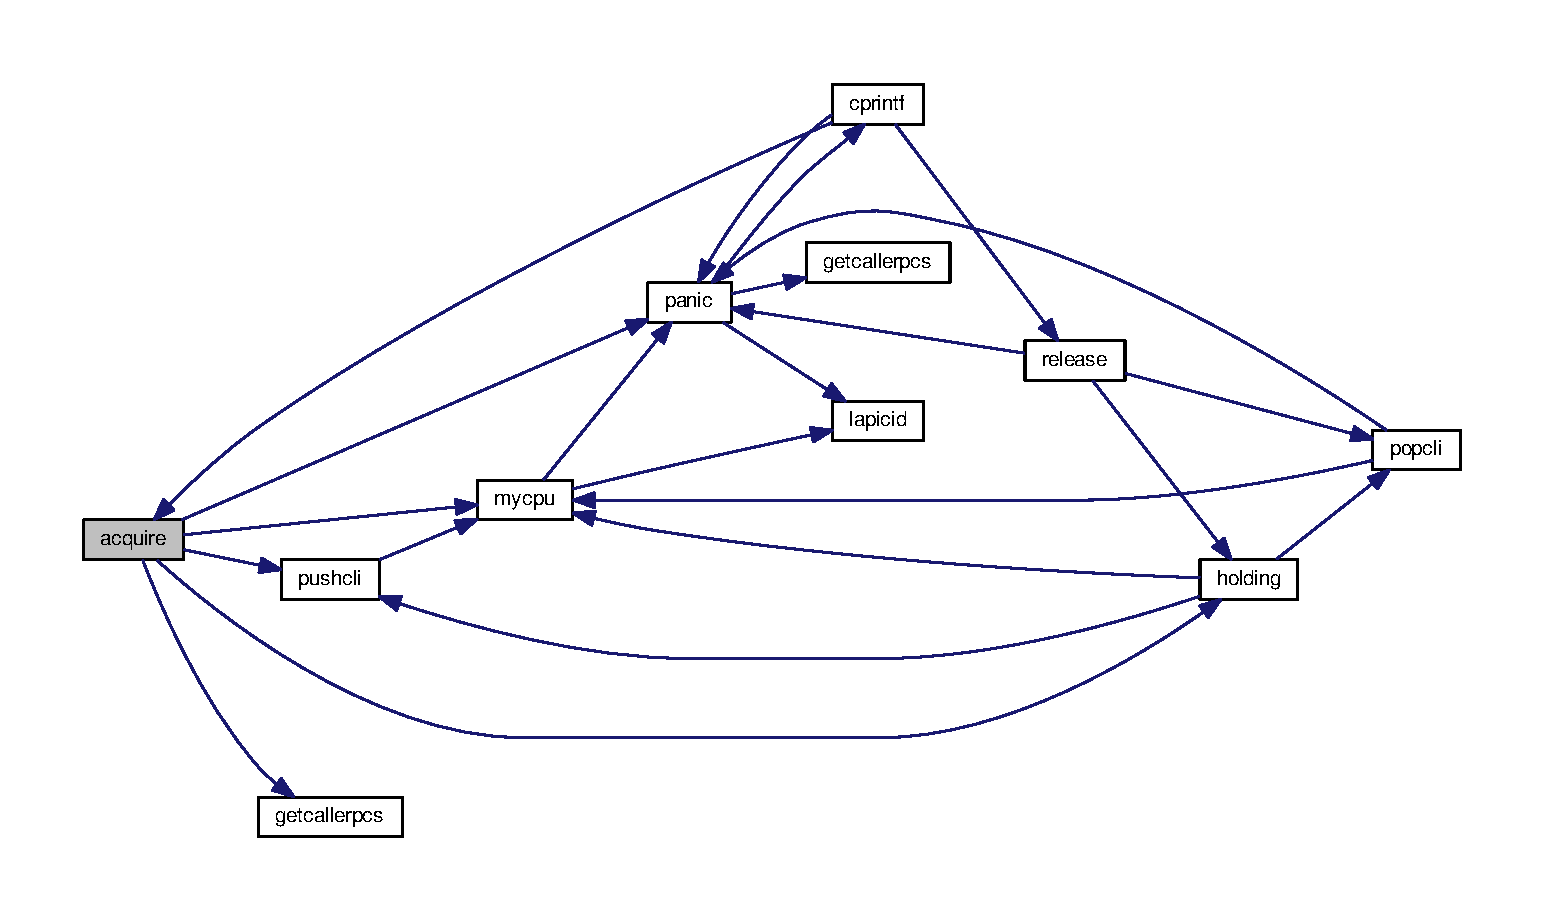
\includegraphics[width=350pt]{d5/d64/defs_8h_afe4ef8638f1ecb962a6e67fb086ee3b8_cgraph}
\end{center}
\end{figure}




Here is the caller graph for this function\+:\nopagebreak
\begin{figure}[H]
\begin{center}
\leavevmode
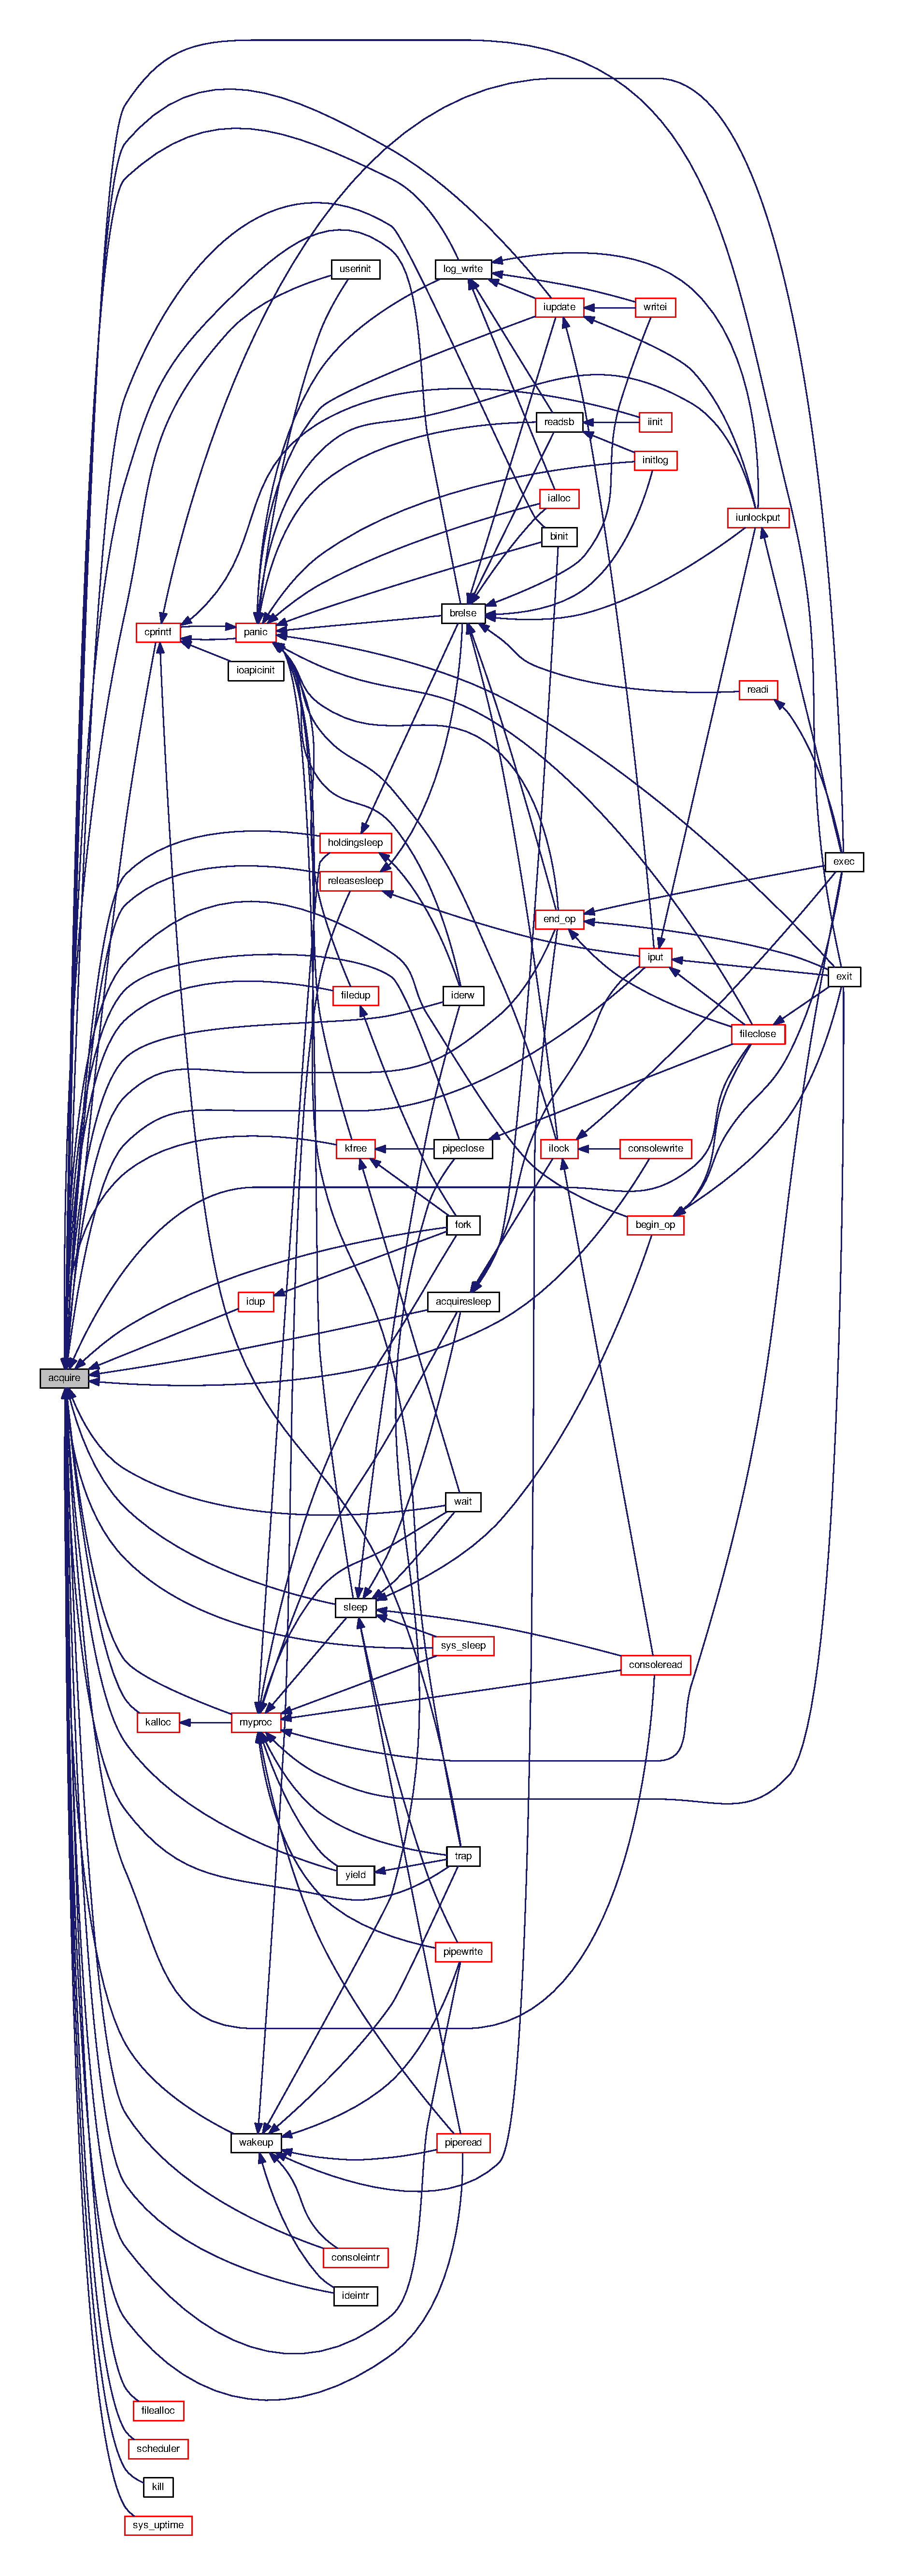
\includegraphics[height=550pt]{d5/d64/defs_8h_afe4ef8638f1ecb962a6e67fb086ee3b8_icgraph}
\end{center}
\end{figure}


\index{defs.\+h@{defs.\+h}!acquiresleep@{acquiresleep}}
\index{acquiresleep@{acquiresleep}!defs.\+h@{defs.\+h}}
\subsubsection[{\texorpdfstring{acquiresleep(struct sleeplock $\ast$)}{acquiresleep(struct sleeplock *)}}]{\setlength{\rightskip}{0pt plus 5cm}void acquiresleep (
\begin{DoxyParamCaption}
\item[{struct {\bf sleeplock} $\ast$}]{}
\end{DoxyParamCaption}
)}\hypertarget{defs_8h_aecd4639fe2f9aaad8e8cee2b5e0688c3}{}\label{defs_8h_aecd4639fe2f9aaad8e8cee2b5e0688c3}


Here is the call graph for this function\+:\nopagebreak
\begin{figure}[H]
\begin{center}
\leavevmode
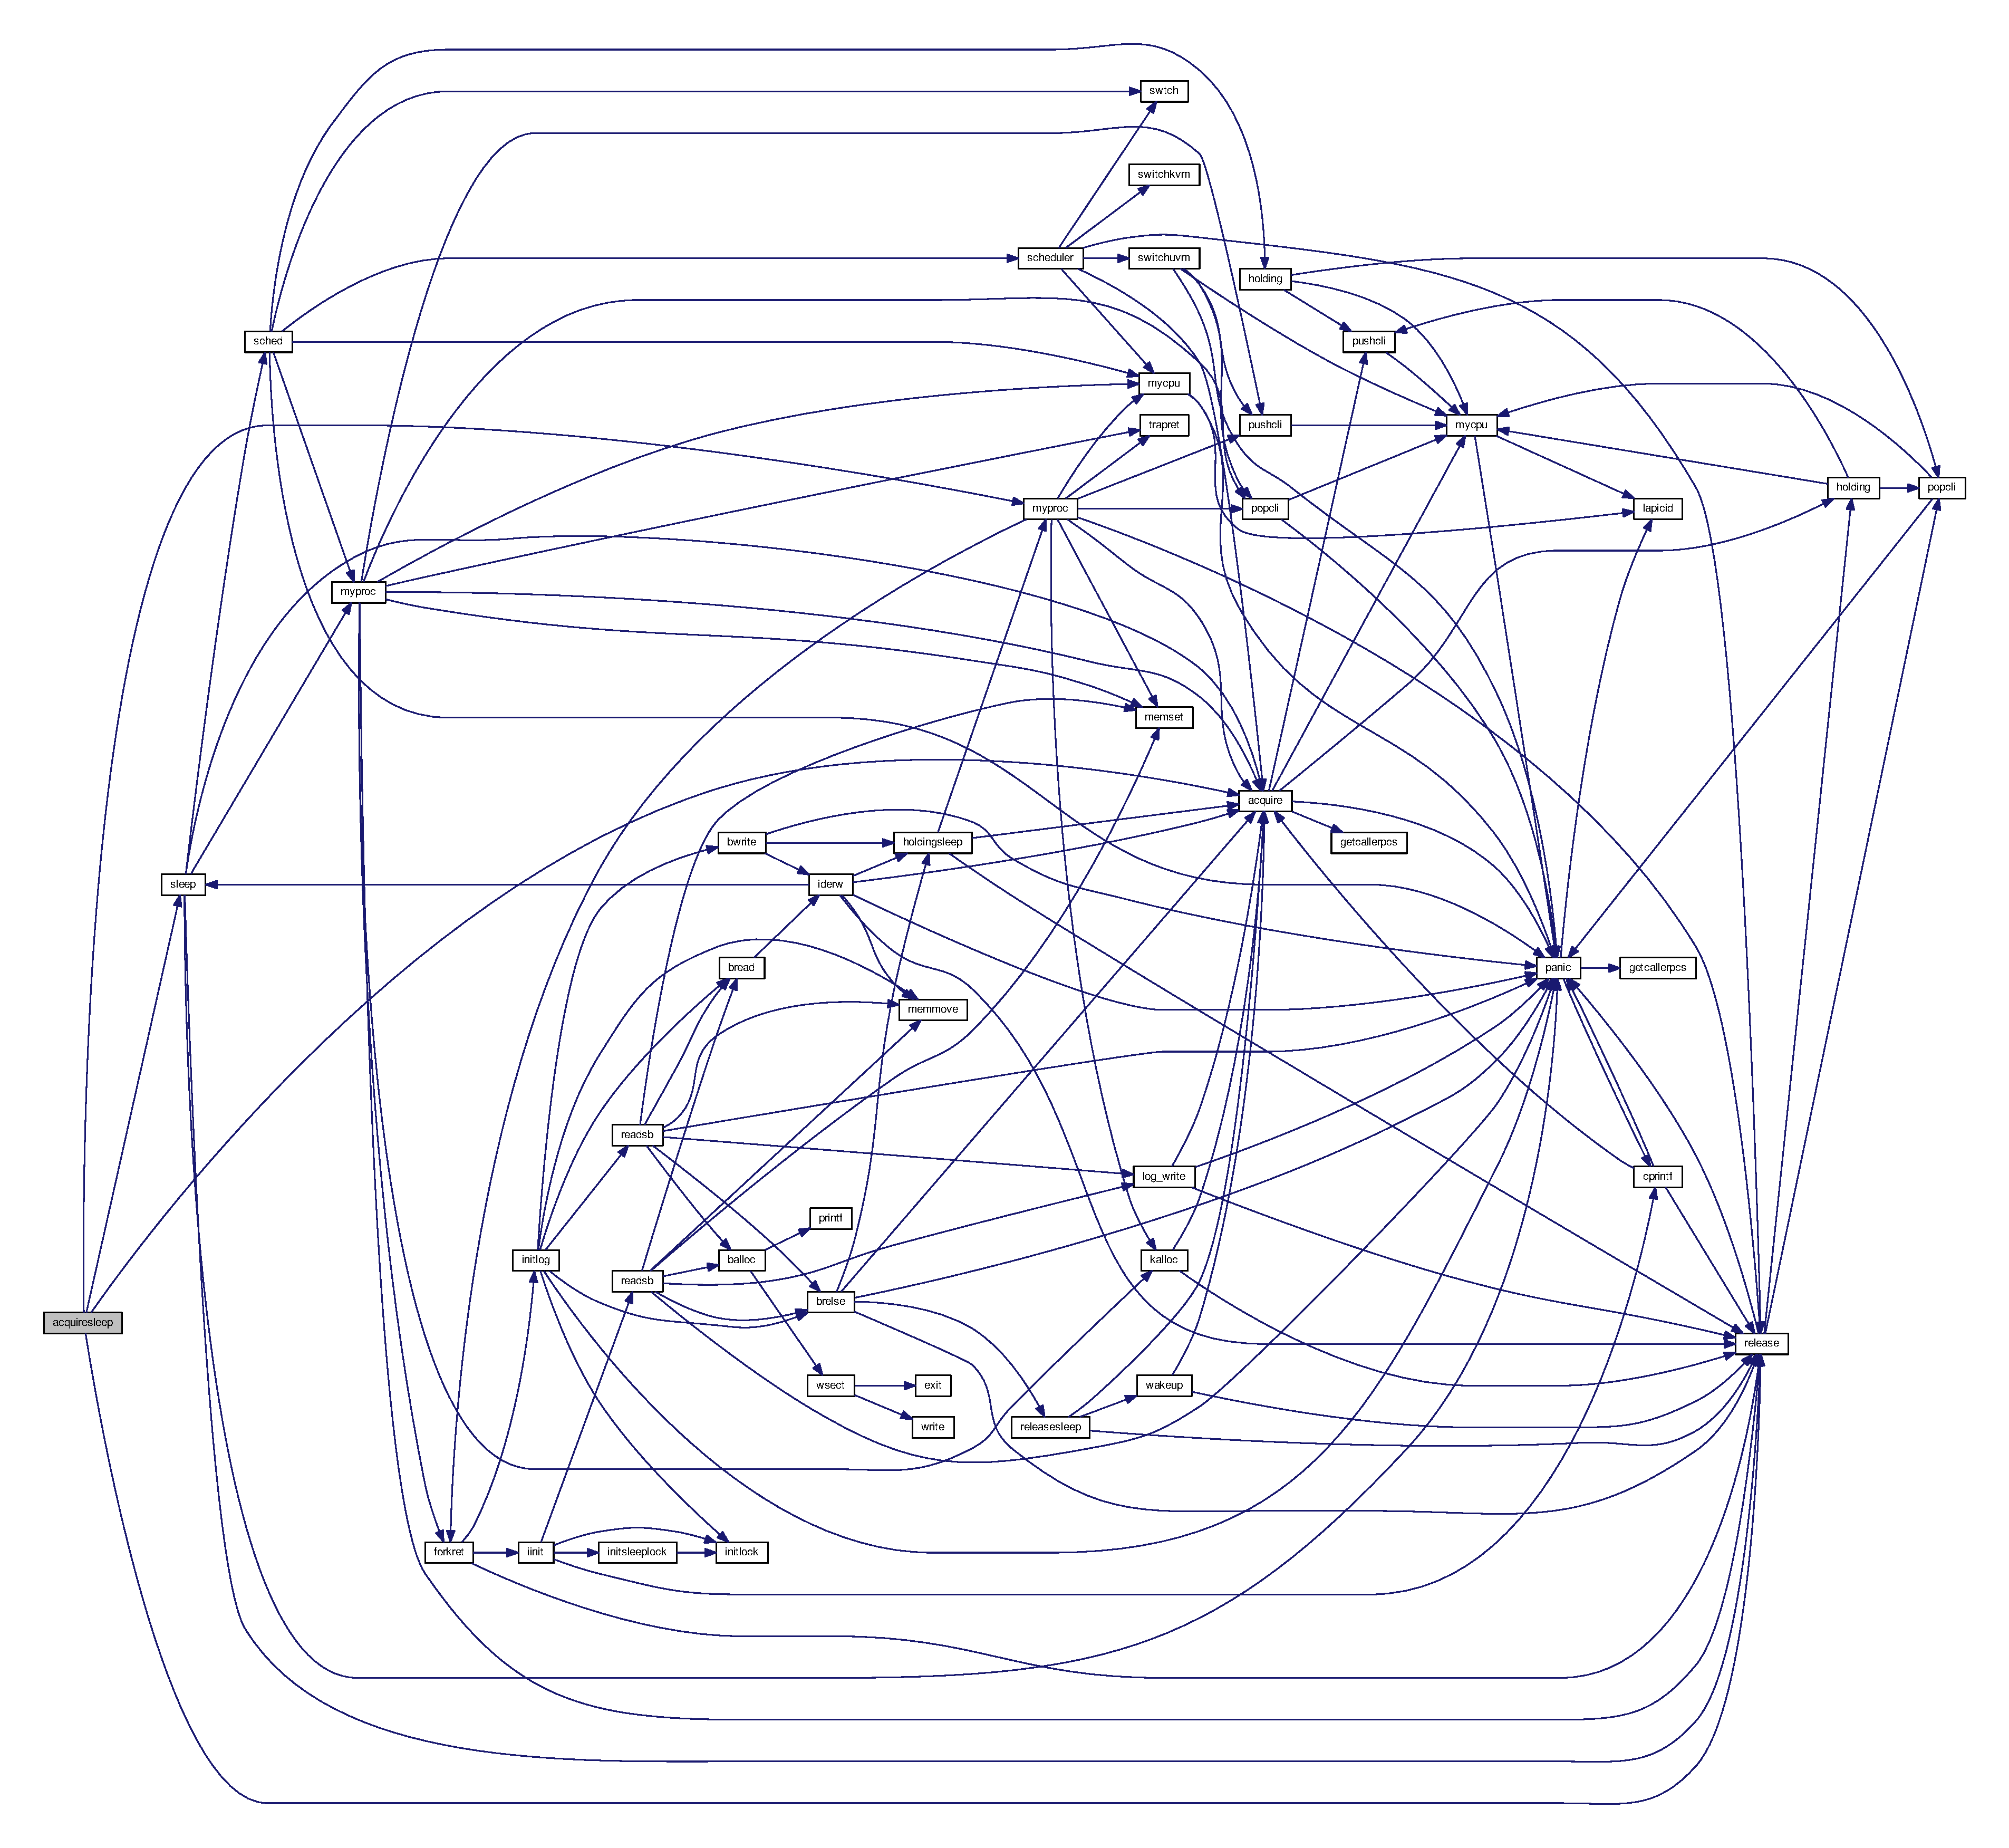
\includegraphics[width=350pt]{d5/d64/defs_8h_aecd4639fe2f9aaad8e8cee2b5e0688c3_cgraph}
\end{center}
\end{figure}




Here is the caller graph for this function\+:\nopagebreak
\begin{figure}[H]
\begin{center}
\leavevmode
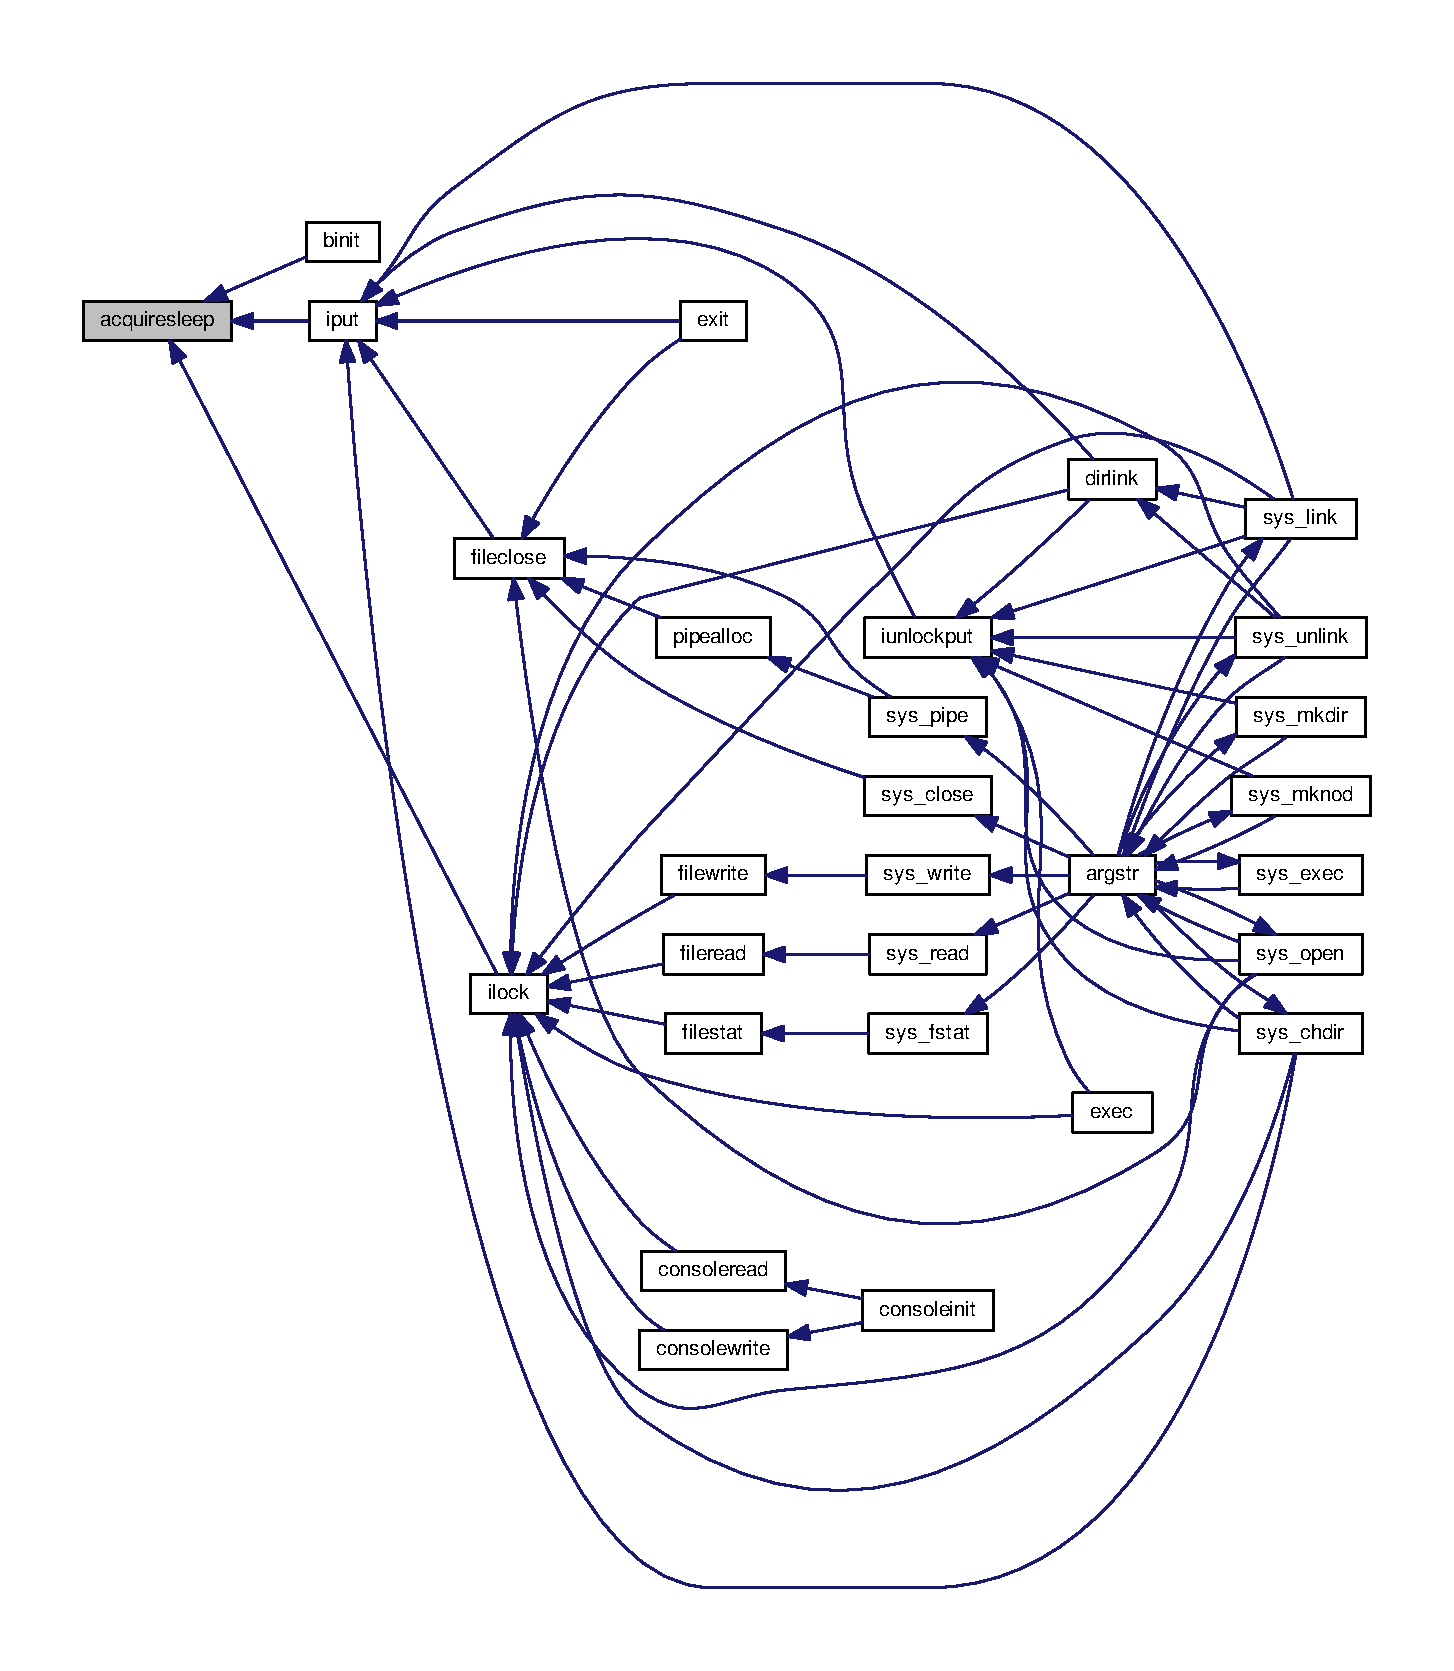
\includegraphics[width=350pt]{d5/d64/defs_8h_aecd4639fe2f9aaad8e8cee2b5e0688c3_icgraph}
\end{center}
\end{figure}


\index{defs.\+h@{defs.\+h}!allocuvm@{allocuvm}}
\index{allocuvm@{allocuvm}!defs.\+h@{defs.\+h}}
\subsubsection[{\texorpdfstring{allocuvm(pde\+\_\+t $\ast$, uint, uint)}{allocuvm(pde_t *, uint, uint)}}]{\setlength{\rightskip}{0pt plus 5cm}int allocuvm (
\begin{DoxyParamCaption}
\item[{{\bf pde\+\_\+t} $\ast$}]{, }
\item[{{\bf uint}}]{, }
\item[{{\bf uint}}]{}
\end{DoxyParamCaption}
)}\hypertarget{defs_8h_a67f50b6f85756f02b5acdcb084d51b9f}{}\label{defs_8h_a67f50b6f85756f02b5acdcb084d51b9f}


Here is the call graph for this function\+:\nopagebreak
\begin{figure}[H]
\begin{center}
\leavevmode
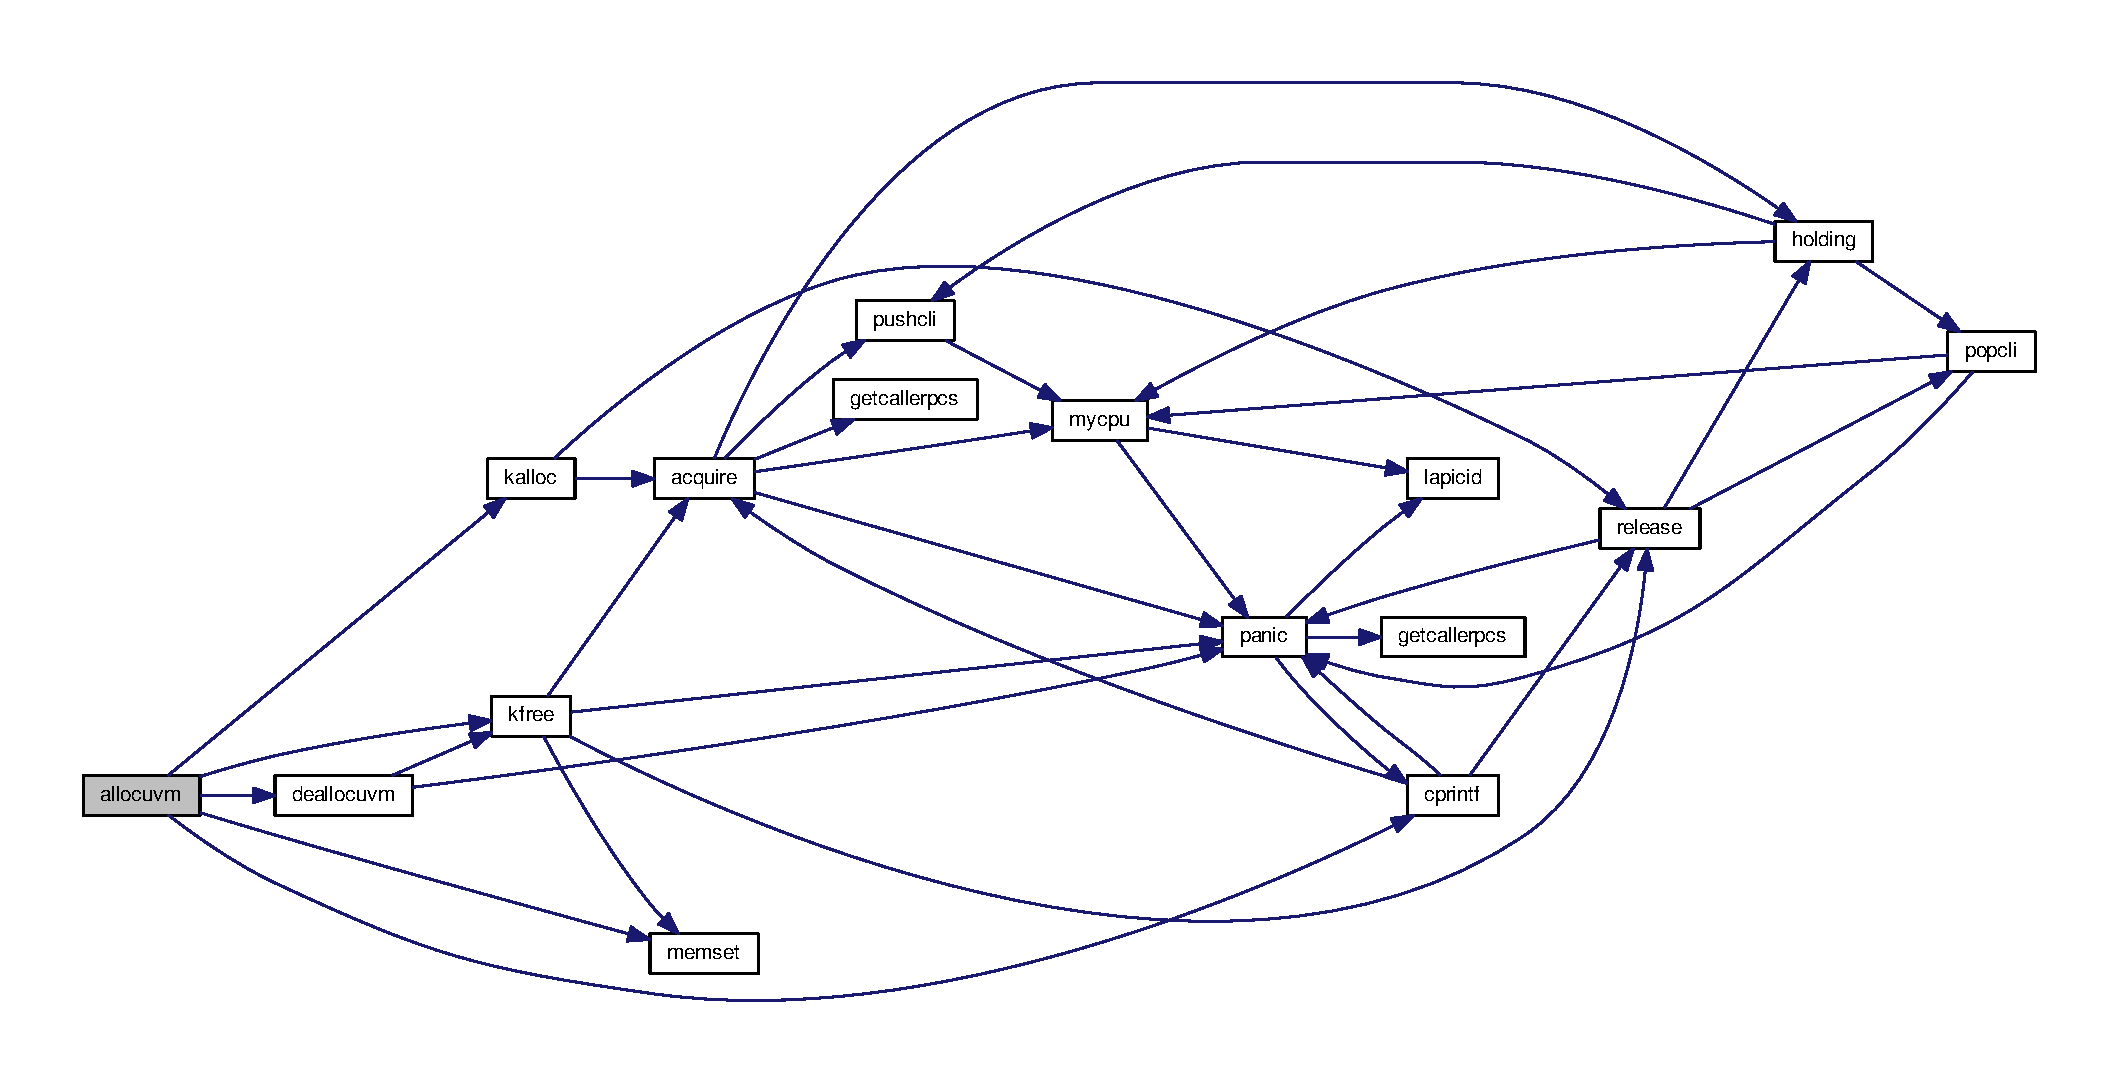
\includegraphics[width=350pt]{d5/d64/defs_8h_a67f50b6f85756f02b5acdcb084d51b9f_cgraph}
\end{center}
\end{figure}




Here is the caller graph for this function\+:\nopagebreak
\begin{figure}[H]
\begin{center}
\leavevmode
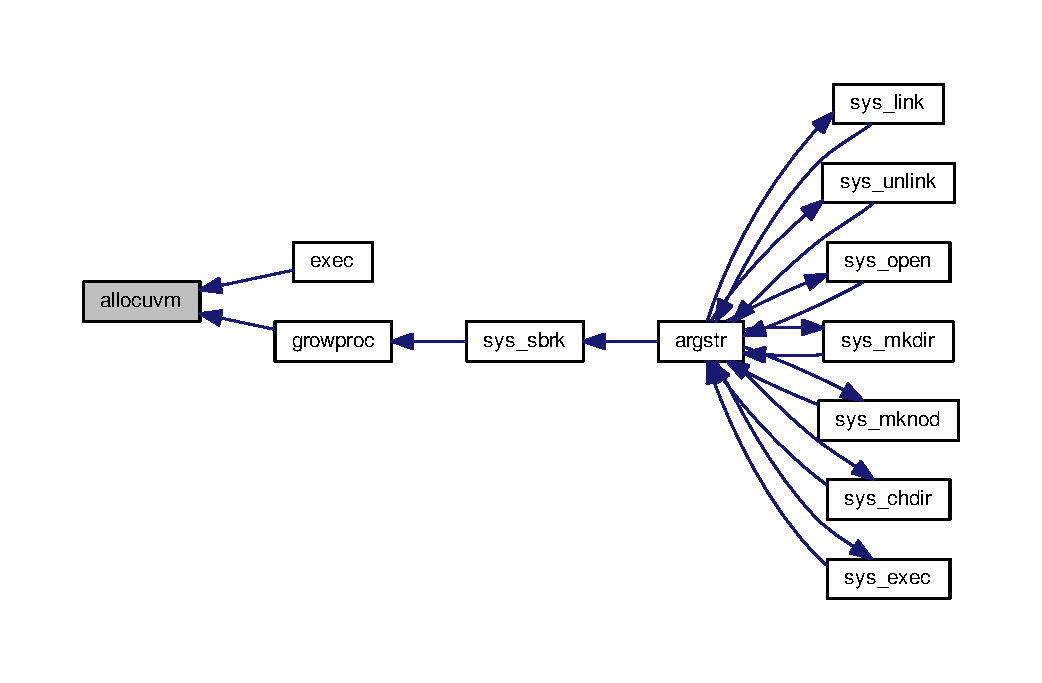
\includegraphics[width=350pt]{d5/d64/defs_8h_a67f50b6f85756f02b5acdcb084d51b9f_icgraph}
\end{center}
\end{figure}


\index{defs.\+h@{defs.\+h}!argint@{argint}}
\index{argint@{argint}!defs.\+h@{defs.\+h}}
\subsubsection[{\texorpdfstring{argint(int, int $\ast$)}{argint(int, int *)}}]{\setlength{\rightskip}{0pt plus 5cm}int argint (
\begin{DoxyParamCaption}
\item[{int}]{, }
\item[{int $\ast$}]{}
\end{DoxyParamCaption}
)}\hypertarget{defs_8h_a75bc8d8c7ea0b4b39d4f470e18e0dba7}{}\label{defs_8h_a75bc8d8c7ea0b4b39d4f470e18e0dba7}


Here is the call graph for this function\+:\nopagebreak
\begin{figure}[H]
\begin{center}
\leavevmode
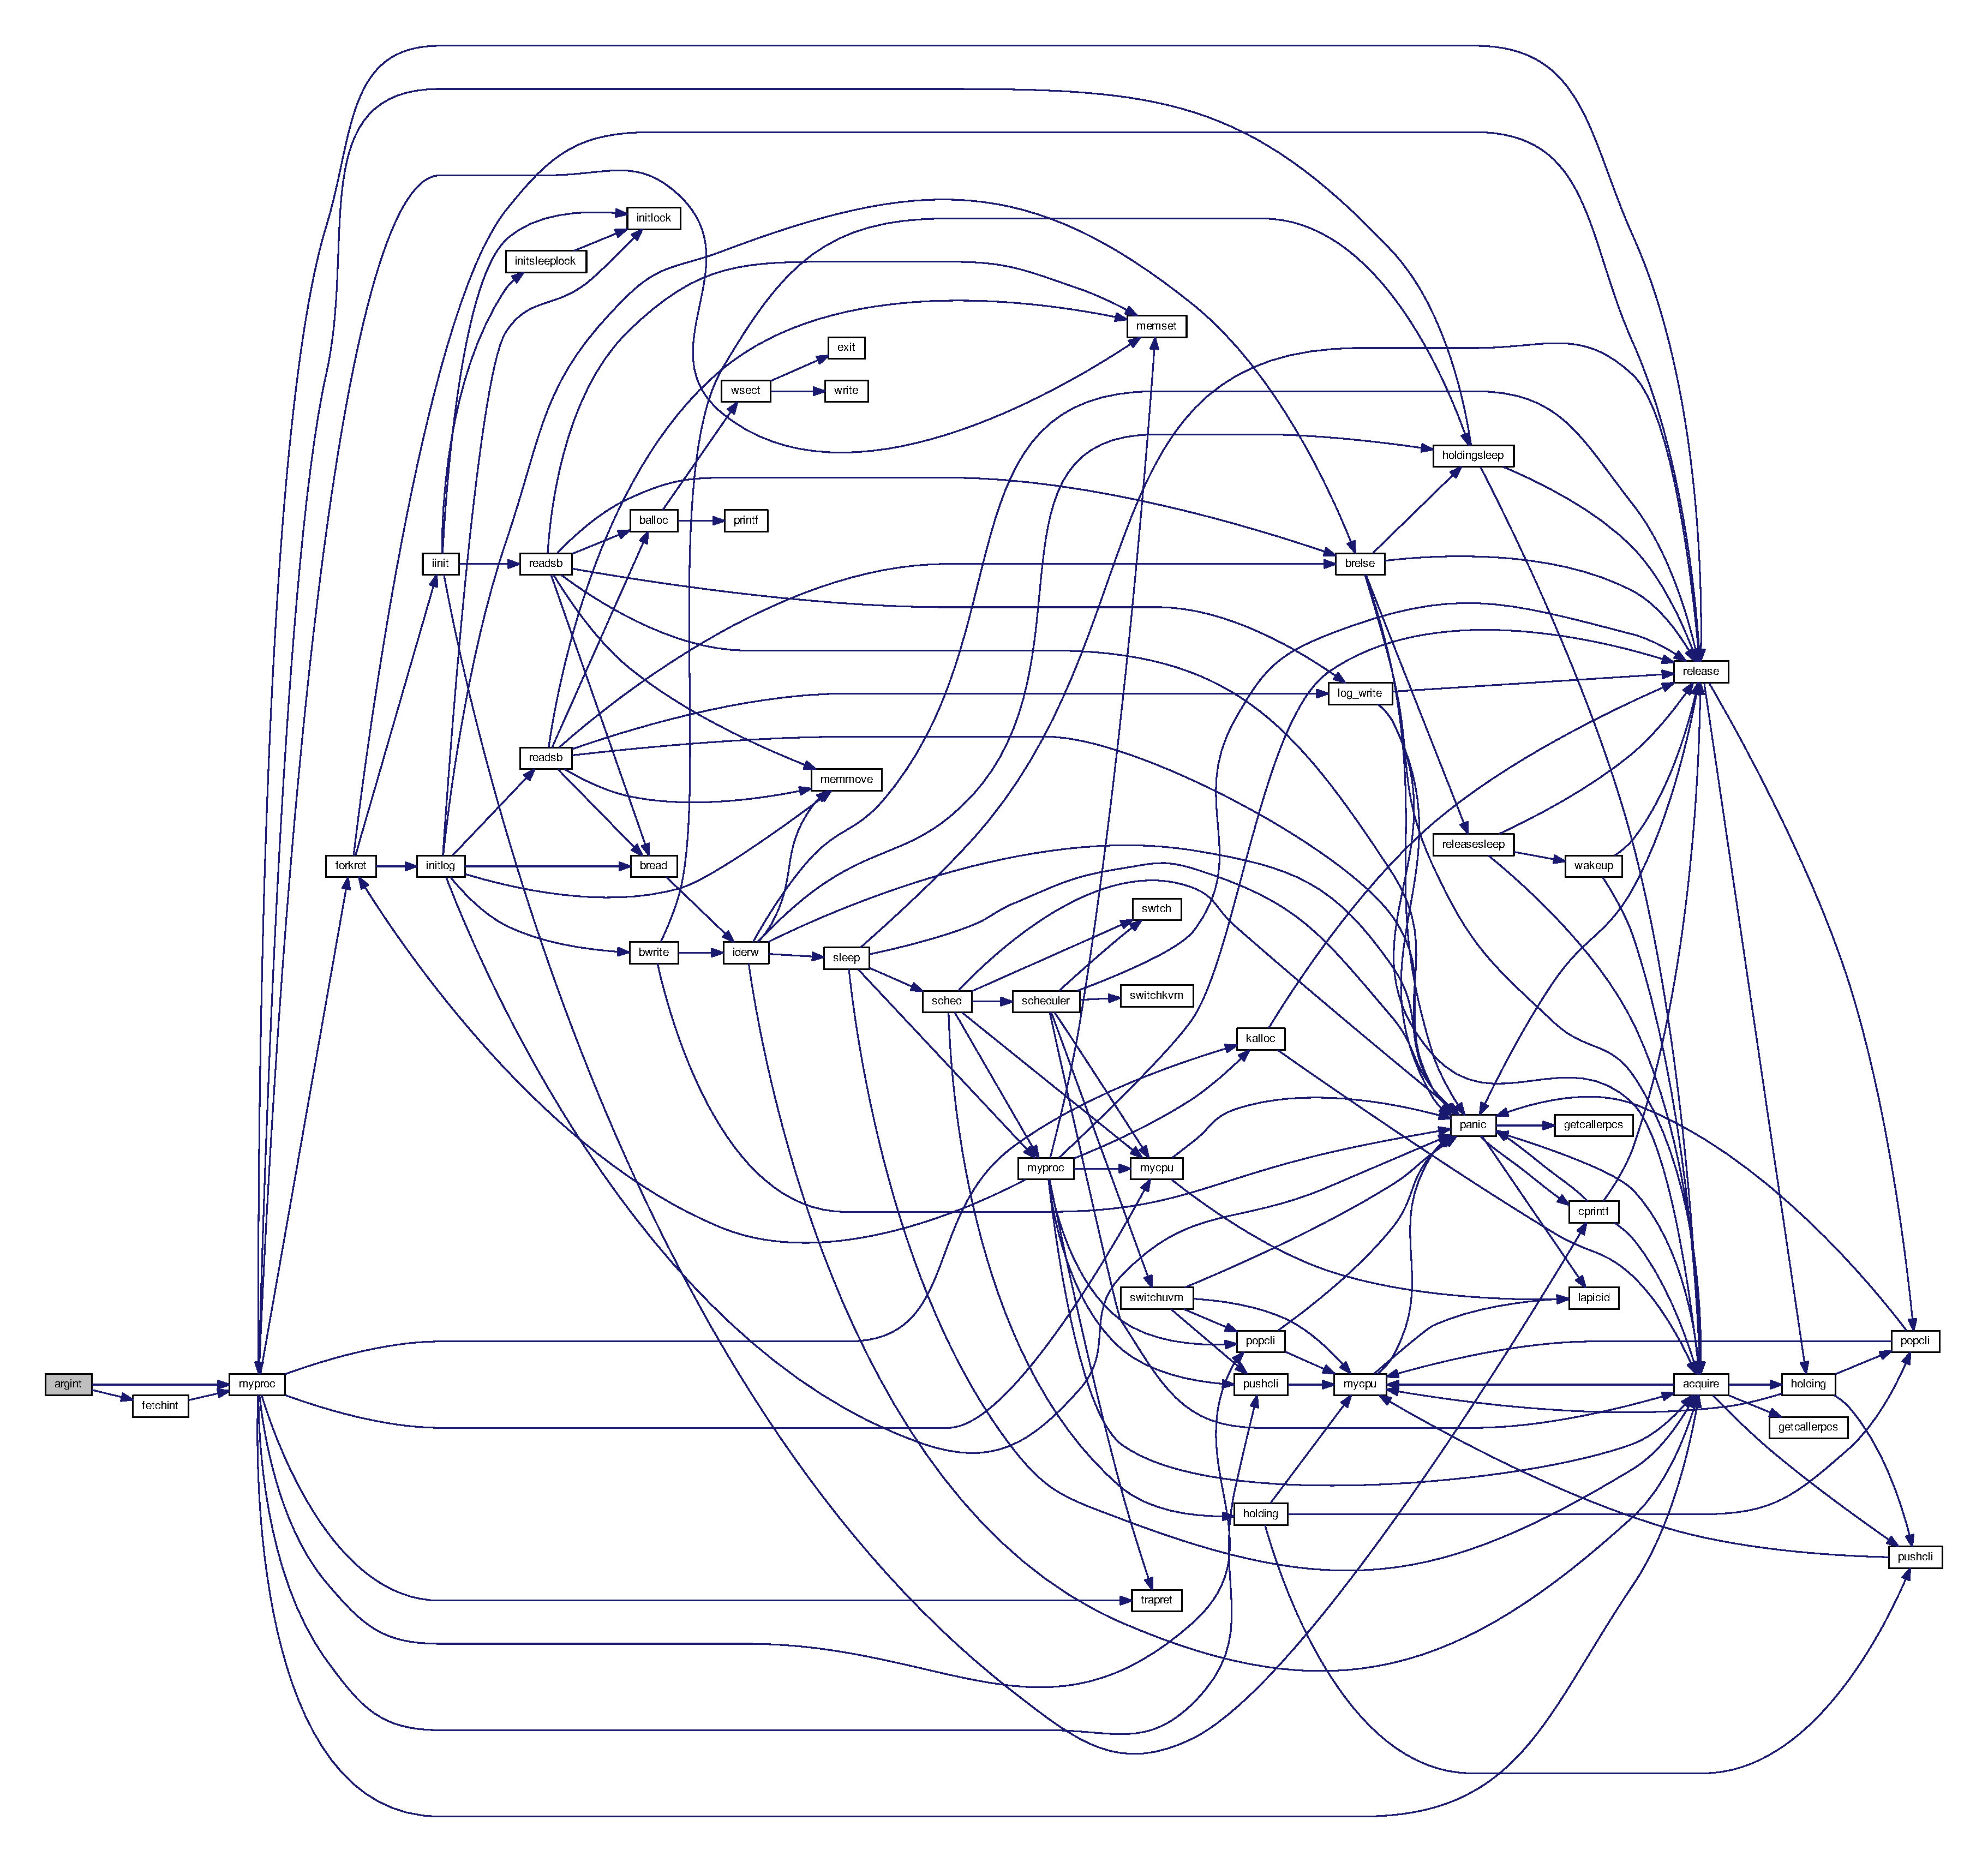
\includegraphics[width=350pt]{d5/d64/defs_8h_a75bc8d8c7ea0b4b39d4f470e18e0dba7_cgraph}
\end{center}
\end{figure}




Here is the caller graph for this function\+:\nopagebreak
\begin{figure}[H]
\begin{center}
\leavevmode
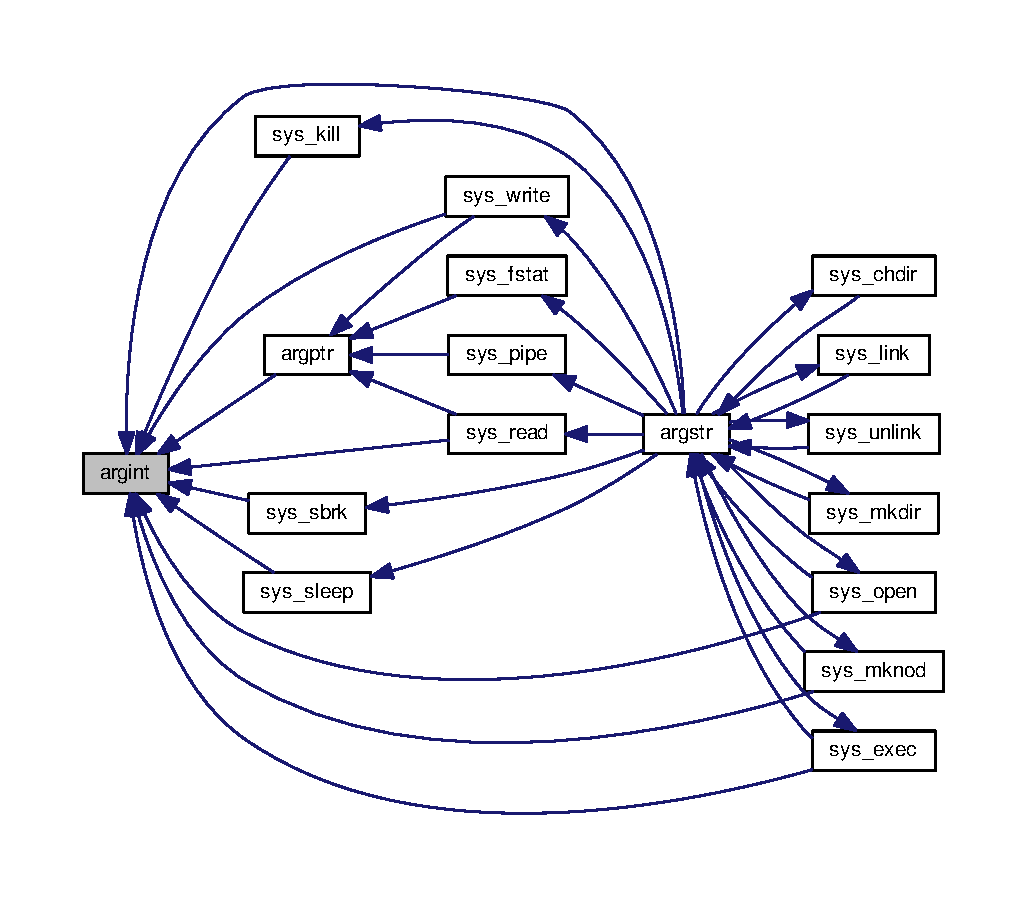
\includegraphics[width=350pt]{d5/d64/defs_8h_a75bc8d8c7ea0b4b39d4f470e18e0dba7_icgraph}
\end{center}
\end{figure}


\index{defs.\+h@{defs.\+h}!argptr@{argptr}}
\index{argptr@{argptr}!defs.\+h@{defs.\+h}}
\subsubsection[{\texorpdfstring{argptr(int, char $\ast$$\ast$, int)}{argptr(int, char **, int)}}]{\setlength{\rightskip}{0pt plus 5cm}int argptr (
\begin{DoxyParamCaption}
\item[{int}]{, }
\item[{char $\ast$$\ast$}]{, }
\item[{int}]{}
\end{DoxyParamCaption}
)}\hypertarget{defs_8h_a05c7464938c27eb91540c06ec6137f26}{}\label{defs_8h_a05c7464938c27eb91540c06ec6137f26}


Here is the call graph for this function\+:\nopagebreak
\begin{figure}[H]
\begin{center}
\leavevmode
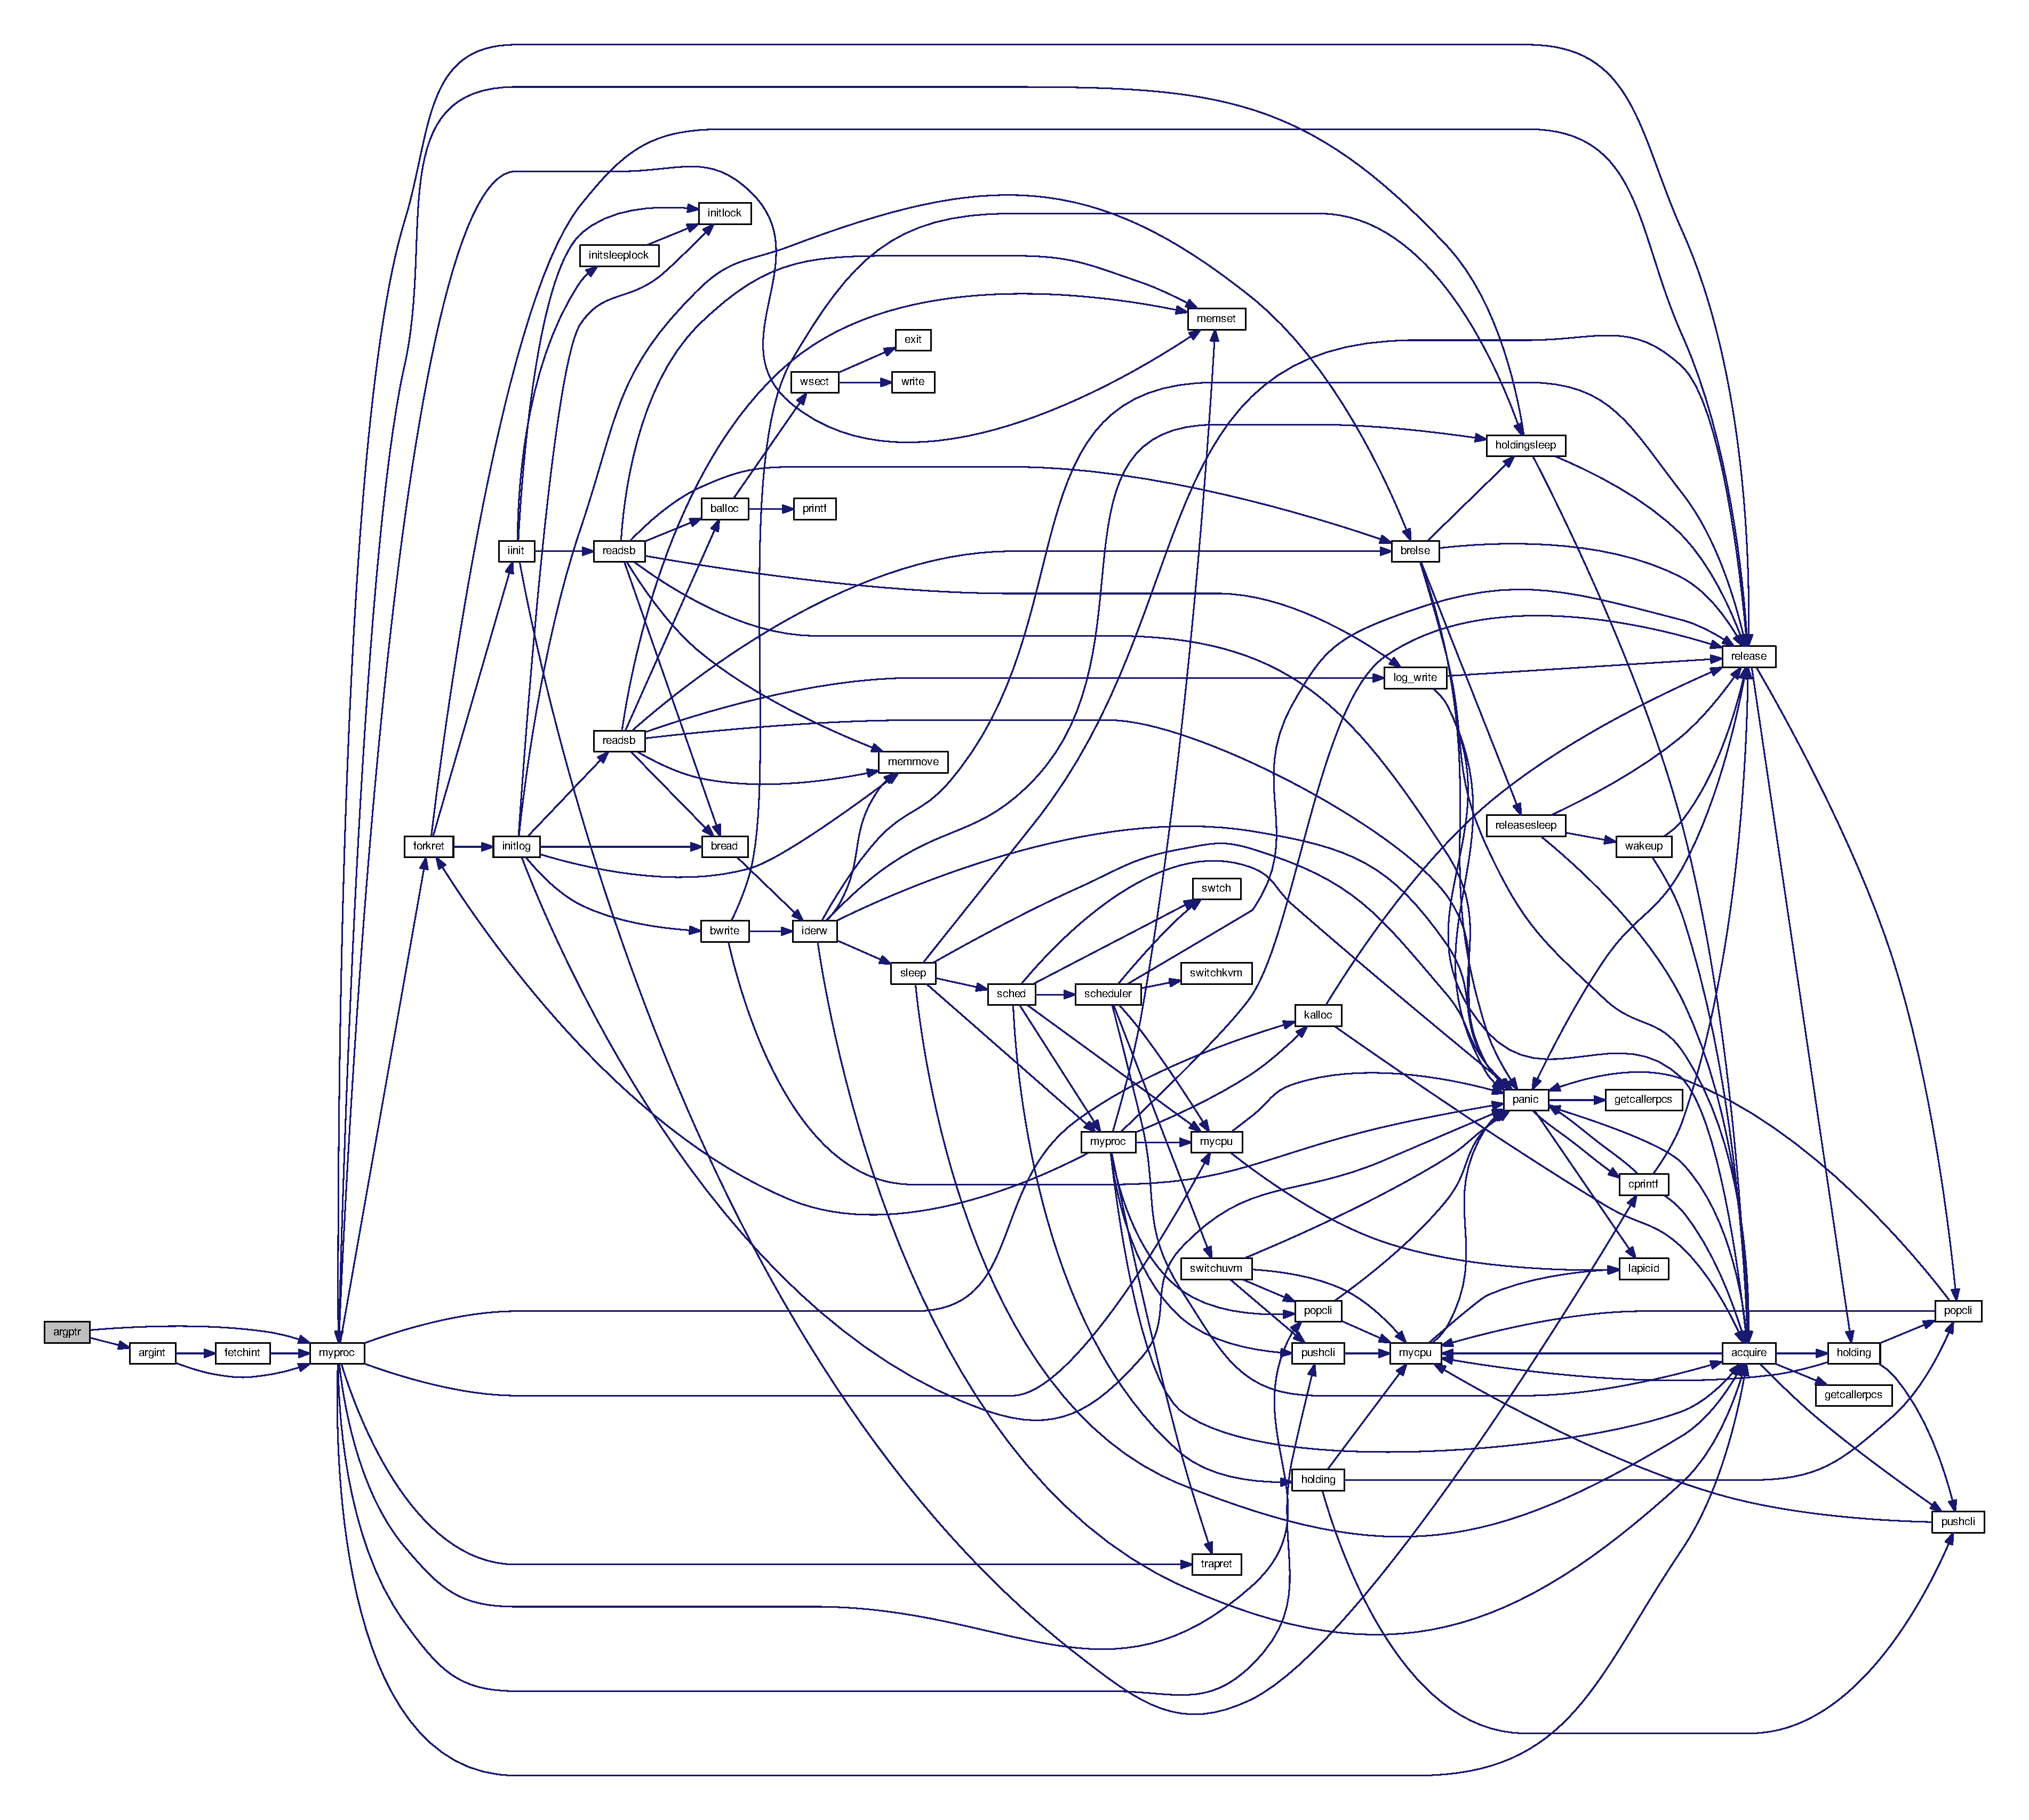
\includegraphics[width=350pt]{d5/d64/defs_8h_a05c7464938c27eb91540c06ec6137f26_cgraph}
\end{center}
\end{figure}




Here is the caller graph for this function\+:\nopagebreak
\begin{figure}[H]
\begin{center}
\leavevmode
\includegraphics[width=350pt]{d5/d64/defs_8h_a05c7464938c27eb91540c06ec6137f26_icgraph}
\end{center}
\end{figure}


\index{defs.\+h@{defs.\+h}!argstr@{argstr}}
\index{argstr@{argstr}!defs.\+h@{defs.\+h}}
\subsubsection[{\texorpdfstring{argstr(int, char $\ast$$\ast$)}{argstr(int, char **)}}]{\setlength{\rightskip}{0pt plus 5cm}int argstr (
\begin{DoxyParamCaption}
\item[{int}]{, }
\item[{char $\ast$$\ast$}]{}
\end{DoxyParamCaption}
)}\hypertarget{defs_8h_afc00cb2e6a06b1021f3d82fa4d0eff07}{}\label{defs_8h_afc00cb2e6a06b1021f3d82fa4d0eff07}


Here is the call graph for this function\+:\nopagebreak
\begin{figure}[H]
\begin{center}
\leavevmode
\includegraphics[height=550pt]{d5/d64/defs_8h_afc00cb2e6a06b1021f3d82fa4d0eff07_cgraph}
\end{center}
\end{figure}




Here is the caller graph for this function\+:\nopagebreak
\begin{figure}[H]
\begin{center}
\leavevmode
\includegraphics[width=350pt]{d5/d64/defs_8h_afc00cb2e6a06b1021f3d82fa4d0eff07_icgraph}
\end{center}
\end{figure}


\index{defs.\+h@{defs.\+h}!begin\+\_\+op@{begin\+\_\+op}}
\index{begin\+\_\+op@{begin\+\_\+op}!defs.\+h@{defs.\+h}}
\subsubsection[{\texorpdfstring{begin\+\_\+op()}{begin_op()}}]{\setlength{\rightskip}{0pt plus 5cm}void begin\+\_\+op (
\begin{DoxyParamCaption}
{}
\end{DoxyParamCaption}
)}\hypertarget{defs_8h_a603ca98212e00d2ffdba7827ef0f1003}{}\label{defs_8h_a603ca98212e00d2ffdba7827ef0f1003}


Here is the call graph for this function\+:\nopagebreak
\begin{figure}[H]
\begin{center}
\leavevmode
\includegraphics[width=350pt]{d5/d64/defs_8h_a603ca98212e00d2ffdba7827ef0f1003_cgraph}
\end{center}
\end{figure}




Here is the caller graph for this function\+:\nopagebreak
\begin{figure}[H]
\begin{center}
\leavevmode
\includegraphics[width=350pt]{d5/d64/defs_8h_a603ca98212e00d2ffdba7827ef0f1003_icgraph}
\end{center}
\end{figure}


\index{defs.\+h@{defs.\+h}!binit@{binit}}
\index{binit@{binit}!defs.\+h@{defs.\+h}}
\subsubsection[{\texorpdfstring{binit(void)}{binit(void)}}]{\setlength{\rightskip}{0pt plus 5cm}void binit (
\begin{DoxyParamCaption}
\item[{void}]{}
\end{DoxyParamCaption}
)}\hypertarget{defs_8h_a53cca0ddc98c5f1de37124eca2575a59}{}\label{defs_8h_a53cca0ddc98c5f1de37124eca2575a59}


Here is the call graph for this function\+:\nopagebreak
\begin{figure}[H]
\begin{center}
\leavevmode
\includegraphics[width=350pt]{d5/d64/defs_8h_a53cca0ddc98c5f1de37124eca2575a59_cgraph}
\end{center}
\end{figure}


\index{defs.\+h@{defs.\+h}!bread@{bread}}
\index{bread@{bread}!defs.\+h@{defs.\+h}}
\subsubsection[{\texorpdfstring{bread(uint, uint)}{bread(uint, uint)}}]{\setlength{\rightskip}{0pt plus 5cm}struct {\bf buf}$\ast$ bread (
\begin{DoxyParamCaption}
\item[{{\bf uint}}]{, }
\item[{{\bf uint}}]{}
\end{DoxyParamCaption}
)}\hypertarget{defs_8h_a90c72cf2140fdf1612484117327220af}{}\label{defs_8h_a90c72cf2140fdf1612484117327220af}


Here is the call graph for this function\+:\nopagebreak
\begin{figure}[H]
\begin{center}
\leavevmode
\includegraphics[width=350pt]{d5/d64/defs_8h_a90c72cf2140fdf1612484117327220af_cgraph}
\end{center}
\end{figure}




Here is the caller graph for this function\+:\nopagebreak
\begin{figure}[H]
\begin{center}
\leavevmode
\includegraphics[width=350pt]{d5/d64/defs_8h_a90c72cf2140fdf1612484117327220af_icgraph}
\end{center}
\end{figure}


\index{defs.\+h@{defs.\+h}!brelse@{brelse}}
\index{brelse@{brelse}!defs.\+h@{defs.\+h}}
\subsubsection[{\texorpdfstring{brelse(struct buf $\ast$)}{brelse(struct buf *)}}]{\setlength{\rightskip}{0pt plus 5cm}void brelse (
\begin{DoxyParamCaption}
\item[{struct {\bf buf} $\ast$}]{}
\end{DoxyParamCaption}
)}\hypertarget{defs_8h_aa31ec2f79e0456737a9680270bc1841b}{}\label{defs_8h_aa31ec2f79e0456737a9680270bc1841b}


Here is the call graph for this function\+:\nopagebreak
\begin{figure}[H]
\begin{center}
\leavevmode
\includegraphics[width=350pt]{d5/d64/defs_8h_aa31ec2f79e0456737a9680270bc1841b_cgraph}
\end{center}
\end{figure}




Here is the caller graph for this function\+:\nopagebreak
\begin{figure}[H]
\begin{center}
\leavevmode
\includegraphics[width=350pt]{d5/d64/defs_8h_aa31ec2f79e0456737a9680270bc1841b_icgraph}
\end{center}
\end{figure}


\index{defs.\+h@{defs.\+h}!bwrite@{bwrite}}
\index{bwrite@{bwrite}!defs.\+h@{defs.\+h}}
\subsubsection[{\texorpdfstring{bwrite(struct buf $\ast$)}{bwrite(struct buf *)}}]{\setlength{\rightskip}{0pt plus 5cm}void bwrite (
\begin{DoxyParamCaption}
\item[{struct {\bf buf} $\ast$}]{}
\end{DoxyParamCaption}
)}\hypertarget{defs_8h_a1bfd775f14ad3dfee354ee3897ecd28d}{}\label{defs_8h_a1bfd775f14ad3dfee354ee3897ecd28d}


Here is the call graph for this function\+:\nopagebreak
\begin{figure}[H]
\begin{center}
\leavevmode
\includegraphics[width=350pt]{d5/d64/defs_8h_a1bfd775f14ad3dfee354ee3897ecd28d_cgraph}
\end{center}
\end{figure}




Here is the caller graph for this function\+:\nopagebreak
\begin{figure}[H]
\begin{center}
\leavevmode
\includegraphics[width=350pt]{d5/d64/defs_8h_a1bfd775f14ad3dfee354ee3897ecd28d_icgraph}
\end{center}
\end{figure}


\index{defs.\+h@{defs.\+h}!clearpteu@{clearpteu}}
\index{clearpteu@{clearpteu}!defs.\+h@{defs.\+h}}
\subsubsection[{\texorpdfstring{clearpteu(pde\+\_\+t $\ast$pgdir, char $\ast$uva)}{clearpteu(pde_t *pgdir, char *uva)}}]{\setlength{\rightskip}{0pt plus 5cm}void clearpteu (
\begin{DoxyParamCaption}
\item[{{\bf pde\+\_\+t} $\ast$}]{pgdir, }
\item[{char $\ast$}]{uva}
\end{DoxyParamCaption}
)}\hypertarget{defs_8h_a795e27a0cb916cfb41411ebbb9669ddf}{}\label{defs_8h_a795e27a0cb916cfb41411ebbb9669ddf}


Here is the call graph for this function\+:\nopagebreak
\begin{figure}[H]
\begin{center}
\leavevmode
\includegraphics[width=350pt]{d5/d64/defs_8h_a795e27a0cb916cfb41411ebbb9669ddf_cgraph}
\end{center}
\end{figure}




Here is the caller graph for this function\+:\nopagebreak
\begin{figure}[H]
\begin{center}
\leavevmode
\includegraphics[width=210pt]{d5/d64/defs_8h_a795e27a0cb916cfb41411ebbb9669ddf_icgraph}
\end{center}
\end{figure}


\index{defs.\+h@{defs.\+h}!cmostime@{cmostime}}
\index{cmostime@{cmostime}!defs.\+h@{defs.\+h}}
\subsubsection[{\texorpdfstring{cmostime(struct rtcdate $\ast$r)}{cmostime(struct rtcdate *r)}}]{\setlength{\rightskip}{0pt plus 5cm}void cmostime (
\begin{DoxyParamCaption}
\item[{struct {\bf rtcdate} $\ast$}]{r}
\end{DoxyParamCaption}
)}\hypertarget{defs_8h_a7247ece9501e31d62cffad46ec33d7af}{}\label{defs_8h_a7247ece9501e31d62cffad46ec33d7af}


Here is the call graph for this function\+:\nopagebreak
\begin{figure}[H]
\begin{center}
\leavevmode
\includegraphics[width=232pt]{d5/d64/defs_8h_a7247ece9501e31d62cffad46ec33d7af_cgraph}
\end{center}
\end{figure}


\index{defs.\+h@{defs.\+h}!consoleinit@{consoleinit}}
\index{consoleinit@{consoleinit}!defs.\+h@{defs.\+h}}
\subsubsection[{\texorpdfstring{consoleinit(void)}{consoleinit(void)}}]{\setlength{\rightskip}{0pt plus 5cm}void consoleinit (
\begin{DoxyParamCaption}
\item[{void}]{}
\end{DoxyParamCaption}
)}\hypertarget{defs_8h_ab508ff0f4db26fe35cd25fa648f9ee75}{}\label{defs_8h_ab508ff0f4db26fe35cd25fa648f9ee75}


Here is the call graph for this function\+:\nopagebreak
\begin{figure}[H]
\begin{center}
\leavevmode
\includegraphics[width=350pt]{d5/d64/defs_8h_ab508ff0f4db26fe35cd25fa648f9ee75_cgraph}
\end{center}
\end{figure}


\index{defs.\+h@{defs.\+h}!consoleintr@{consoleintr}}
\index{consoleintr@{consoleintr}!defs.\+h@{defs.\+h}}
\subsubsection[{\texorpdfstring{consoleintr(int($\ast$)(void))}{consoleintr(int(*)(void))}}]{\setlength{\rightskip}{0pt plus 5cm}void consoleintr (
\begin{DoxyParamCaption}
\item[{int($\ast$)(void)}]{}
\end{DoxyParamCaption}
)}\hypertarget{defs_8h_a9ec968a6fc407075634fe0e82a9c6862}{}\label{defs_8h_a9ec968a6fc407075634fe0e82a9c6862}


Here is the call graph for this function\+:\nopagebreak
\begin{figure}[H]
\begin{center}
\leavevmode
\includegraphics[width=350pt]{d5/d64/defs_8h_a9ec968a6fc407075634fe0e82a9c6862_cgraph}
\end{center}
\end{figure}




Here is the caller graph for this function\+:\nopagebreak
\begin{figure}[H]
\begin{center}
\leavevmode
\includegraphics[width=296pt]{d5/d64/defs_8h_a9ec968a6fc407075634fe0e82a9c6862_icgraph}
\end{center}
\end{figure}


\index{defs.\+h@{defs.\+h}!copyout@{copyout}}
\index{copyout@{copyout}!defs.\+h@{defs.\+h}}
\subsubsection[{\texorpdfstring{copyout(pde\+\_\+t $\ast$, uint, void $\ast$, uint)}{copyout(pde_t *, uint, void *, uint)}}]{\setlength{\rightskip}{0pt plus 5cm}int copyout (
\begin{DoxyParamCaption}
\item[{{\bf pde\+\_\+t} $\ast$}]{, }
\item[{{\bf uint}}]{, }
\item[{void $\ast$}]{, }
\item[{{\bf uint}}]{}
\end{DoxyParamCaption}
)}\hypertarget{defs_8h_a11f5ff2e5bcd16968a88fcbb30db5a10}{}\label{defs_8h_a11f5ff2e5bcd16968a88fcbb30db5a10}


Here is the call graph for this function\+:\nopagebreak
\begin{figure}[H]
\begin{center}
\leavevmode
\includegraphics[width=229pt]{d5/d64/defs_8h_a11f5ff2e5bcd16968a88fcbb30db5a10_cgraph}
\end{center}
\end{figure}




Here is the caller graph for this function\+:\nopagebreak
\begin{figure}[H]
\begin{center}
\leavevmode
\includegraphics[width=205pt]{d5/d64/defs_8h_a11f5ff2e5bcd16968a88fcbb30db5a10_icgraph}
\end{center}
\end{figure}


\index{defs.\+h@{defs.\+h}!copyuvm@{copyuvm}}
\index{copyuvm@{copyuvm}!defs.\+h@{defs.\+h}}
\subsubsection[{\texorpdfstring{copyuvm(pde\+\_\+t $\ast$, uint)}{copyuvm(pde_t *, uint)}}]{\setlength{\rightskip}{0pt plus 5cm}{\bf pde\+\_\+t}$\ast$ copyuvm (
\begin{DoxyParamCaption}
\item[{{\bf pde\+\_\+t} $\ast$}]{, }
\item[{{\bf uint}}]{}
\end{DoxyParamCaption}
)}\hypertarget{defs_8h_aaa9d4abe019ce435b9a3296be3a2e214}{}\label{defs_8h_aaa9d4abe019ce435b9a3296be3a2e214}


Here is the call graph for this function\+:\nopagebreak
\begin{figure}[H]
\begin{center}
\leavevmode
\includegraphics[width=350pt]{d5/d64/defs_8h_aaa9d4abe019ce435b9a3296be3a2e214_cgraph}
\end{center}
\end{figure}




Here is the caller graph for this function\+:\nopagebreak
\begin{figure}[H]
\begin{center}
\leavevmode
\includegraphics[width=205pt]{d5/d64/defs_8h_aaa9d4abe019ce435b9a3296be3a2e214_icgraph}
\end{center}
\end{figure}


\index{defs.\+h@{defs.\+h}!cprintf@{cprintf}}
\index{cprintf@{cprintf}!defs.\+h@{defs.\+h}}
\subsubsection[{\texorpdfstring{cprintf(char $\ast$,...)}{cprintf(char *,...)}}]{\setlength{\rightskip}{0pt plus 5cm}void cprintf (
\begin{DoxyParamCaption}
\item[{char $\ast$}]{, }
\item[{}]{...}
\end{DoxyParamCaption}
)}\hypertarget{defs_8h_abeb2bc020e7332bcde1d7beab08582d3}{}\label{defs_8h_abeb2bc020e7332bcde1d7beab08582d3}


Here is the call graph for this function\+:\nopagebreak
\begin{figure}[H]
\begin{center}
\leavevmode
\includegraphics[width=350pt]{d5/d64/defs_8h_abeb2bc020e7332bcde1d7beab08582d3_cgraph}
\end{center}
\end{figure}




Here is the caller graph for this function\+:\nopagebreak
\begin{figure}[H]
\begin{center}
\leavevmode
\includegraphics[height=550pt]{d5/d64/defs_8h_abeb2bc020e7332bcde1d7beab08582d3_icgraph}
\end{center}
\end{figure}


\index{defs.\+h@{defs.\+h}!cpuid@{cpuid}}
\index{cpuid@{cpuid}!defs.\+h@{defs.\+h}}
\subsubsection[{\texorpdfstring{cpuid(void)}{cpuid(void)}}]{\setlength{\rightskip}{0pt plus 5cm}int cpuid (
\begin{DoxyParamCaption}
\item[{void}]{}
\end{DoxyParamCaption}
)}\hypertarget{defs_8h_a1444de2903d3d2624a50de058d19c635}{}\label{defs_8h_a1444de2903d3d2624a50de058d19c635}


Here is the call graph for this function\+:\nopagebreak
\begin{figure}[H]
\begin{center}
\leavevmode
\includegraphics[width=350pt]{d5/d64/defs_8h_a1444de2903d3d2624a50de058d19c635_cgraph}
\end{center}
\end{figure}




Here is the caller graph for this function\+:\nopagebreak
\begin{figure}[H]
\begin{center}
\leavevmode
\includegraphics[width=201pt]{d5/d64/defs_8h_a1444de2903d3d2624a50de058d19c635_icgraph}
\end{center}
\end{figure}


\index{defs.\+h@{defs.\+h}!deallocuvm@{deallocuvm}}
\index{deallocuvm@{deallocuvm}!defs.\+h@{defs.\+h}}
\subsubsection[{\texorpdfstring{deallocuvm(pde\+\_\+t $\ast$, uint, uint)}{deallocuvm(pde_t *, uint, uint)}}]{\setlength{\rightskip}{0pt plus 5cm}int deallocuvm (
\begin{DoxyParamCaption}
\item[{{\bf pde\+\_\+t} $\ast$}]{, }
\item[{{\bf uint}}]{, }
\item[{{\bf uint}}]{}
\end{DoxyParamCaption}
)}\hypertarget{defs_8h_ac45969a8875b6dc87245e0a642aa2d8d}{}\label{defs_8h_ac45969a8875b6dc87245e0a642aa2d8d}


Here is the call graph for this function\+:\nopagebreak
\begin{figure}[H]
\begin{center}
\leavevmode
\includegraphics[width=350pt]{d5/d64/defs_8h_ac45969a8875b6dc87245e0a642aa2d8d_cgraph}
\end{center}
\end{figure}




Here is the caller graph for this function\+:\nopagebreak
\begin{figure}[H]
\begin{center}
\leavevmode
\includegraphics[width=350pt]{d5/d64/defs_8h_ac45969a8875b6dc87245e0a642aa2d8d_icgraph}
\end{center}
\end{figure}


\index{defs.\+h@{defs.\+h}!dirlink@{dirlink}}
\index{dirlink@{dirlink}!defs.\+h@{defs.\+h}}
\subsubsection[{\texorpdfstring{dirlink(struct inode $\ast$, char $\ast$, uint)}{dirlink(struct inode *, char *, uint)}}]{\setlength{\rightskip}{0pt plus 5cm}int dirlink (
\begin{DoxyParamCaption}
\item[{struct {\bf inode} $\ast$}]{, }
\item[{char $\ast$}]{, }
\item[{{\bf uint}}]{}
\end{DoxyParamCaption}
)}\hypertarget{defs_8h_ae4ccea0aa02557162963e597737f665a}{}\label{defs_8h_ae4ccea0aa02557162963e597737f665a}


Here is the call graph for this function\+:\nopagebreak
\begin{figure}[H]
\begin{center}
\leavevmode
\includegraphics[width=350pt]{d5/d64/defs_8h_ae4ccea0aa02557162963e597737f665a_cgraph}
\end{center}
\end{figure}




Here is the caller graph for this function\+:\nopagebreak
\begin{figure}[H]
\begin{center}
\leavevmode
\includegraphics[width=350pt]{d5/d64/defs_8h_ae4ccea0aa02557162963e597737f665a_icgraph}
\end{center}
\end{figure}


\index{defs.\+h@{defs.\+h}!dirlookup@{dirlookup}}
\index{dirlookup@{dirlookup}!defs.\+h@{defs.\+h}}
\subsubsection[{\texorpdfstring{dirlookup(struct inode $\ast$, char $\ast$, uint $\ast$)}{dirlookup(struct inode *, char *, uint *)}}]{\setlength{\rightskip}{0pt plus 5cm}struct {\bf inode}$\ast$ dirlookup (
\begin{DoxyParamCaption}
\item[{struct {\bf inode} $\ast$}]{, }
\item[{char $\ast$}]{, }
\item[{{\bf uint} $\ast$}]{}
\end{DoxyParamCaption}
)}\hypertarget{defs_8h_a91ded9e61402d5e0d9f16b2a8cbff5c3}{}\label{defs_8h_a91ded9e61402d5e0d9f16b2a8cbff5c3}


Here is the call graph for this function\+:\nopagebreak
\begin{figure}[H]
\begin{center}
\leavevmode
\includegraphics[width=350pt]{d5/d64/defs_8h_a91ded9e61402d5e0d9f16b2a8cbff5c3_cgraph}
\end{center}
\end{figure}




Here is the caller graph for this function\+:\nopagebreak
\begin{figure}[H]
\begin{center}
\leavevmode
\includegraphics[width=350pt]{d5/d64/defs_8h_a91ded9e61402d5e0d9f16b2a8cbff5c3_icgraph}
\end{center}
\end{figure}


\index{defs.\+h@{defs.\+h}!end\+\_\+op@{end\+\_\+op}}
\index{end\+\_\+op@{end\+\_\+op}!defs.\+h@{defs.\+h}}
\subsubsection[{\texorpdfstring{end\+\_\+op()}{end_op()}}]{\setlength{\rightskip}{0pt plus 5cm}void end\+\_\+op (
\begin{DoxyParamCaption}
{}
\end{DoxyParamCaption}
)}\hypertarget{defs_8h_a2504e37a109f9bae5ca11fe89e4e8fa1}{}\label{defs_8h_a2504e37a109f9bae5ca11fe89e4e8fa1}


Here is the call graph for this function\+:\nopagebreak
\begin{figure}[H]
\begin{center}
\leavevmode
\includegraphics[width=350pt]{d5/d64/defs_8h_a2504e37a109f9bae5ca11fe89e4e8fa1_cgraph}
\end{center}
\end{figure}




Here is the caller graph for this function\+:\nopagebreak
\begin{figure}[H]
\begin{center}
\leavevmode
\includegraphics[width=350pt]{d5/d64/defs_8h_a2504e37a109f9bae5ca11fe89e4e8fa1_icgraph}
\end{center}
\end{figure}


\index{defs.\+h@{defs.\+h}!exec@{exec}}
\index{exec@{exec}!defs.\+h@{defs.\+h}}
\subsubsection[{\texorpdfstring{exec(char $\ast$, char $\ast$$\ast$)}{exec(char *, char **)}}]{\setlength{\rightskip}{0pt plus 5cm}int exec (
\begin{DoxyParamCaption}
\item[{char $\ast$}]{, }
\item[{char $\ast$$\ast$}]{}
\end{DoxyParamCaption}
)}\hypertarget{defs_8h_aa7b4aae4a12acd187e23396214aeca47}{}\label{defs_8h_aa7b4aae4a12acd187e23396214aeca47}


Here is the caller graph for this function\+:\nopagebreak
\begin{figure}[H]
\begin{center}
\leavevmode
\includegraphics[width=350pt]{d5/d64/defs_8h_aa7b4aae4a12acd187e23396214aeca47_icgraph}
\end{center}
\end{figure}


\index{defs.\+h@{defs.\+h}!exit@{exit}}
\index{exit@{exit}!defs.\+h@{defs.\+h}}
\subsubsection[{\texorpdfstring{exit(void)}{exit(void)}}]{\setlength{\rightskip}{0pt plus 5cm}void exit (
\begin{DoxyParamCaption}
\item[{void}]{}
\end{DoxyParamCaption}
)}\hypertarget{defs_8h_aaf98ef7cdde3a0dfb2e49919de3298b1}{}\label{defs_8h_aaf98ef7cdde3a0dfb2e49919de3298b1}


Here is the caller graph for this function\+:\nopagebreak
\begin{figure}[H]
\begin{center}
\leavevmode
\includegraphics[width=350pt]{d5/d64/defs_8h_aaf98ef7cdde3a0dfb2e49919de3298b1_icgraph}
\end{center}
\end{figure}


\index{defs.\+h@{defs.\+h}!fetchint@{fetchint}}
\index{fetchint@{fetchint}!defs.\+h@{defs.\+h}}
\subsubsection[{\texorpdfstring{fetchint(uint, int $\ast$)}{fetchint(uint, int *)}}]{\setlength{\rightskip}{0pt plus 5cm}int fetchint (
\begin{DoxyParamCaption}
\item[{{\bf uint}}]{, }
\item[{int $\ast$}]{}
\end{DoxyParamCaption}
)}\hypertarget{defs_8h_ab8c95490fad429ac2701653041f2efcf}{}\label{defs_8h_ab8c95490fad429ac2701653041f2efcf}


Here is the call graph for this function\+:\nopagebreak
\begin{figure}[H]
\begin{center}
\leavevmode
\includegraphics[width=350pt]{d5/d64/defs_8h_ab8c95490fad429ac2701653041f2efcf_cgraph}
\end{center}
\end{figure}




Here is the caller graph for this function\+:\nopagebreak
\begin{figure}[H]
\begin{center}
\leavevmode
\includegraphics[width=350pt]{d5/d64/defs_8h_ab8c95490fad429ac2701653041f2efcf_icgraph}
\end{center}
\end{figure}


\index{defs.\+h@{defs.\+h}!fetchstr@{fetchstr}}
\index{fetchstr@{fetchstr}!defs.\+h@{defs.\+h}}
\subsubsection[{\texorpdfstring{fetchstr(uint, char $\ast$$\ast$)}{fetchstr(uint, char **)}}]{\setlength{\rightskip}{0pt plus 5cm}int fetchstr (
\begin{DoxyParamCaption}
\item[{{\bf uint}}]{, }
\item[{char $\ast$$\ast$}]{}
\end{DoxyParamCaption}
)}\hypertarget{defs_8h_a386d969a02c926521cf2e1816069a4dc}{}\label{defs_8h_a386d969a02c926521cf2e1816069a4dc}


Here is the call graph for this function\+:\nopagebreak
\begin{figure}[H]
\begin{center}
\leavevmode
\includegraphics[width=350pt]{d5/d64/defs_8h_a386d969a02c926521cf2e1816069a4dc_cgraph}
\end{center}
\end{figure}




Here is the caller graph for this function\+:\nopagebreak
\begin{figure}[H]
\begin{center}
\leavevmode
\includegraphics[width=310pt]{d5/d64/defs_8h_a386d969a02c926521cf2e1816069a4dc_icgraph}
\end{center}
\end{figure}


\index{defs.\+h@{defs.\+h}!filealloc@{filealloc}}
\index{filealloc@{filealloc}!defs.\+h@{defs.\+h}}
\subsubsection[{\texorpdfstring{filealloc(void)}{filealloc(void)}}]{\setlength{\rightskip}{0pt plus 5cm}struct {\bf file}$\ast$ filealloc (
\begin{DoxyParamCaption}
\item[{void}]{}
\end{DoxyParamCaption}
)}\hypertarget{defs_8h_a69d3d2dd94efa1f1ff8d0143f4d9b786}{}\label{defs_8h_a69d3d2dd94efa1f1ff8d0143f4d9b786}


Here is the call graph for this function\+:\nopagebreak
\begin{figure}[H]
\begin{center}
\leavevmode
\includegraphics[width=350pt]{d5/d64/defs_8h_a69d3d2dd94efa1f1ff8d0143f4d9b786_cgraph}
\end{center}
\end{figure}




Here is the caller graph for this function\+:\nopagebreak
\begin{figure}[H]
\begin{center}
\leavevmode
\includegraphics[width=350pt]{d5/d64/defs_8h_a69d3d2dd94efa1f1ff8d0143f4d9b786_icgraph}
\end{center}
\end{figure}


\index{defs.\+h@{defs.\+h}!fileclose@{fileclose}}
\index{fileclose@{fileclose}!defs.\+h@{defs.\+h}}
\subsubsection[{\texorpdfstring{fileclose(struct file $\ast$)}{fileclose(struct file *)}}]{\setlength{\rightskip}{0pt plus 5cm}void fileclose (
\begin{DoxyParamCaption}
\item[{struct {\bf file} $\ast$}]{}
\end{DoxyParamCaption}
)}\hypertarget{defs_8h_ac865ee0b2d70f753d61d1fefef9de0f6}{}\label{defs_8h_ac865ee0b2d70f753d61d1fefef9de0f6}


Here is the call graph for this function\+:\nopagebreak
\begin{figure}[H]
\begin{center}
\leavevmode
\includegraphics[width=350pt]{d5/d64/defs_8h_ac865ee0b2d70f753d61d1fefef9de0f6_cgraph}
\end{center}
\end{figure}




Here is the caller graph for this function\+:\nopagebreak
\begin{figure}[H]
\begin{center}
\leavevmode
\includegraphics[width=350pt]{d5/d64/defs_8h_ac865ee0b2d70f753d61d1fefef9de0f6_icgraph}
\end{center}
\end{figure}


\index{defs.\+h@{defs.\+h}!filedup@{filedup}}
\index{filedup@{filedup}!defs.\+h@{defs.\+h}}
\subsubsection[{\texorpdfstring{filedup(struct file $\ast$)}{filedup(struct file *)}}]{\setlength{\rightskip}{0pt plus 5cm}struct {\bf file}$\ast$ filedup (
\begin{DoxyParamCaption}
\item[{struct {\bf file} $\ast$}]{}
\end{DoxyParamCaption}
)}\hypertarget{defs_8h_a1063546fe0d5f45fe1a38a9b4f6b5783}{}\label{defs_8h_a1063546fe0d5f45fe1a38a9b4f6b5783}


Here is the call graph for this function\+:\nopagebreak
\begin{figure}[H]
\begin{center}
\leavevmode
\includegraphics[width=350pt]{d5/d64/defs_8h_a1063546fe0d5f45fe1a38a9b4f6b5783_cgraph}
\end{center}
\end{figure}




Here is the caller graph for this function\+:\nopagebreak
\begin{figure}[H]
\begin{center}
\leavevmode
\includegraphics[width=350pt]{d5/d64/defs_8h_a1063546fe0d5f45fe1a38a9b4f6b5783_icgraph}
\end{center}
\end{figure}


\index{defs.\+h@{defs.\+h}!fileinit@{fileinit}}
\index{fileinit@{fileinit}!defs.\+h@{defs.\+h}}
\subsubsection[{\texorpdfstring{fileinit(void)}{fileinit(void)}}]{\setlength{\rightskip}{0pt plus 5cm}void fileinit (
\begin{DoxyParamCaption}
\item[{void}]{}
\end{DoxyParamCaption}
)}\hypertarget{defs_8h_a66bb5a4b304ea0f851dd999fc8195fa4}{}\label{defs_8h_a66bb5a4b304ea0f851dd999fc8195fa4}


Here is the call graph for this function\+:\nopagebreak
\begin{figure}[H]
\begin{center}
\leavevmode
\includegraphics[width=205pt]{d5/d64/defs_8h_a66bb5a4b304ea0f851dd999fc8195fa4_cgraph}
\end{center}
\end{figure}


\index{defs.\+h@{defs.\+h}!fileread@{fileread}}
\index{fileread@{fileread}!defs.\+h@{defs.\+h}}
\subsubsection[{\texorpdfstring{fileread(struct file $\ast$, char $\ast$, int n)}{fileread(struct file *, char *, int n)}}]{\setlength{\rightskip}{0pt plus 5cm}int fileread (
\begin{DoxyParamCaption}
\item[{struct {\bf file} $\ast$}]{, }
\item[{char $\ast$}]{, }
\item[{int}]{n}
\end{DoxyParamCaption}
)}\hypertarget{defs_8h_a6bd1db179155944c9d1fbc89d8b7b162}{}\label{defs_8h_a6bd1db179155944c9d1fbc89d8b7b162}


Here is the call graph for this function\+:\nopagebreak
\begin{figure}[H]
\begin{center}
\leavevmode
\includegraphics[width=350pt]{d5/d64/defs_8h_a6bd1db179155944c9d1fbc89d8b7b162_cgraph}
\end{center}
\end{figure}




Here is the caller graph for this function\+:\nopagebreak
\begin{figure}[H]
\begin{center}
\leavevmode
\includegraphics[width=350pt]{d5/d64/defs_8h_a6bd1db179155944c9d1fbc89d8b7b162_icgraph}
\end{center}
\end{figure}


\index{defs.\+h@{defs.\+h}!filestat@{filestat}}
\index{filestat@{filestat}!defs.\+h@{defs.\+h}}
\subsubsection[{\texorpdfstring{filestat(struct file $\ast$, struct stat $\ast$)}{filestat(struct file *, struct stat *)}}]{\setlength{\rightskip}{0pt plus 5cm}int filestat (
\begin{DoxyParamCaption}
\item[{struct {\bf file} $\ast$}]{, }
\item[{struct {\bf stat} $\ast$}]{}
\end{DoxyParamCaption}
)}\hypertarget{defs_8h_ac4979f97957194db01001985b1bfa84e}{}\label{defs_8h_ac4979f97957194db01001985b1bfa84e}


Here is the call graph for this function\+:\nopagebreak
\begin{figure}[H]
\begin{center}
\leavevmode
\includegraphics[width=350pt]{d5/d64/defs_8h_ac4979f97957194db01001985b1bfa84e_cgraph}
\end{center}
\end{figure}




Here is the caller graph for this function\+:\nopagebreak
\begin{figure}[H]
\begin{center}
\leavevmode
\includegraphics[width=350pt]{d5/d64/defs_8h_ac4979f97957194db01001985b1bfa84e_icgraph}
\end{center}
\end{figure}


\index{defs.\+h@{defs.\+h}!filewrite@{filewrite}}
\index{filewrite@{filewrite}!defs.\+h@{defs.\+h}}
\subsubsection[{\texorpdfstring{filewrite(struct file $\ast$, char $\ast$, int n)}{filewrite(struct file *, char *, int n)}}]{\setlength{\rightskip}{0pt plus 5cm}int filewrite (
\begin{DoxyParamCaption}
\item[{struct {\bf file} $\ast$}]{, }
\item[{char $\ast$}]{, }
\item[{int}]{n}
\end{DoxyParamCaption}
)}\hypertarget{defs_8h_a90e8980df48fa900fc33de53448a2e18}{}\label{defs_8h_a90e8980df48fa900fc33de53448a2e18}


Here is the call graph for this function\+:\nopagebreak
\begin{figure}[H]
\begin{center}
\leavevmode
\includegraphics[width=350pt]{d5/d64/defs_8h_a90e8980df48fa900fc33de53448a2e18_cgraph}
\end{center}
\end{figure}




Here is the caller graph for this function\+:\nopagebreak
\begin{figure}[H]
\begin{center}
\leavevmode
\includegraphics[width=350pt]{d5/d64/defs_8h_a90e8980df48fa900fc33de53448a2e18_icgraph}
\end{center}
\end{figure}


\index{defs.\+h@{defs.\+h}!fork@{fork}}
\index{fork@{fork}!defs.\+h@{defs.\+h}}
\subsubsection[{\texorpdfstring{fork(void)}{fork(void)}}]{\setlength{\rightskip}{0pt plus 5cm}int fork (
\begin{DoxyParamCaption}
\item[{void}]{}
\end{DoxyParamCaption}
)}\hypertarget{defs_8h_acd2e1ded4bb6fce4500438bf928330f4}{}\label{defs_8h_acd2e1ded4bb6fce4500438bf928330f4}


Here is the caller graph for this function\+:\nopagebreak
\begin{figure}[H]
\begin{center}
\leavevmode
\includegraphics[width=350pt]{d5/d64/defs_8h_acd2e1ded4bb6fce4500438bf928330f4_icgraph}
\end{center}
\end{figure}


\index{defs.\+h@{defs.\+h}!freevm@{freevm}}
\index{freevm@{freevm}!defs.\+h@{defs.\+h}}
\subsubsection[{\texorpdfstring{freevm(pde\+\_\+t $\ast$)}{freevm(pde_t *)}}]{\setlength{\rightskip}{0pt plus 5cm}void freevm (
\begin{DoxyParamCaption}
\item[{{\bf pde\+\_\+t} $\ast$}]{}
\end{DoxyParamCaption}
)}\hypertarget{defs_8h_af24cf1756e19afd8be8c95d02262cf3a}{}\label{defs_8h_af24cf1756e19afd8be8c95d02262cf3a}


Here is the call graph for this function\+:\nopagebreak
\begin{figure}[H]
\begin{center}
\leavevmode
\includegraphics[width=350pt]{d5/d64/defs_8h_af24cf1756e19afd8be8c95d02262cf3a_cgraph}
\end{center}
\end{figure}




Here is the caller graph for this function\+:\nopagebreak
\begin{figure}[H]
\begin{center}
\leavevmode
\includegraphics[width=350pt]{d5/d64/defs_8h_af24cf1756e19afd8be8c95d02262cf3a_icgraph}
\end{center}
\end{figure}


\index{defs.\+h@{defs.\+h}!getcallerpcs@{getcallerpcs}}
\index{getcallerpcs@{getcallerpcs}!defs.\+h@{defs.\+h}}
\subsubsection[{\texorpdfstring{getcallerpcs(void $\ast$, uint $\ast$)}{getcallerpcs(void *, uint *)}}]{\setlength{\rightskip}{0pt plus 5cm}void getcallerpcs (
\begin{DoxyParamCaption}
\item[{void $\ast$}]{, }
\item[{{\bf uint} $\ast$}]{}
\end{DoxyParamCaption}
)}\hypertarget{defs_8h_a4105de9e2969515d6c6c795c4386f69f}{}\label{defs_8h_a4105de9e2969515d6c6c795c4386f69f}


Here is the caller graph for this function\+:\nopagebreak
\begin{figure}[H]
\begin{center}
\leavevmode
\includegraphics[height=550pt]{d5/d64/defs_8h_a4105de9e2969515d6c6c795c4386f69f_icgraph}
\end{center}
\end{figure}


\index{defs.\+h@{defs.\+h}!growproc@{growproc}}
\index{growproc@{growproc}!defs.\+h@{defs.\+h}}
\subsubsection[{\texorpdfstring{growproc(int)}{growproc(int)}}]{\setlength{\rightskip}{0pt plus 5cm}int growproc (
\begin{DoxyParamCaption}
\item[{int}]{}
\end{DoxyParamCaption}
)}\hypertarget{defs_8h_acb02e9289fb8a1017c3455b137a9bccd}{}\label{defs_8h_acb02e9289fb8a1017c3455b137a9bccd}


Here is the call graph for this function\+:\nopagebreak
\begin{figure}[H]
\begin{center}
\leavevmode
\includegraphics[width=350pt]{d5/d64/defs_8h_acb02e9289fb8a1017c3455b137a9bccd_cgraph}
\end{center}
\end{figure}




Here is the caller graph for this function\+:\nopagebreak
\begin{figure}[H]
\begin{center}
\leavevmode
\includegraphics[width=350pt]{d5/d64/defs_8h_acb02e9289fb8a1017c3455b137a9bccd_icgraph}
\end{center}
\end{figure}


\index{defs.\+h@{defs.\+h}!holding@{holding}}
\index{holding@{holding}!defs.\+h@{defs.\+h}}
\subsubsection[{\texorpdfstring{holding(struct spinlock $\ast$)}{holding(struct spinlock *)}}]{\setlength{\rightskip}{0pt plus 5cm}int holding (
\begin{DoxyParamCaption}
\item[{struct {\bf spinlock} $\ast$}]{}
\end{DoxyParamCaption}
)}\hypertarget{defs_8h_ac44b13cc76bf4040e3baf34df75ff230}{}\label{defs_8h_ac44b13cc76bf4040e3baf34df75ff230}


Here is the call graph for this function\+:\nopagebreak
\begin{figure}[H]
\begin{center}
\leavevmode
\includegraphics[width=350pt]{d5/d64/defs_8h_ac44b13cc76bf4040e3baf34df75ff230_cgraph}
\end{center}
\end{figure}




Here is the caller graph for this function\+:\nopagebreak
\begin{figure}[H]
\begin{center}
\leavevmode
\includegraphics[height=550pt]{d5/d64/defs_8h_ac44b13cc76bf4040e3baf34df75ff230_icgraph}
\end{center}
\end{figure}


\index{defs.\+h@{defs.\+h}!holdingsleep@{holdingsleep}}
\index{holdingsleep@{holdingsleep}!defs.\+h@{defs.\+h}}
\subsubsection[{\texorpdfstring{holdingsleep(struct sleeplock $\ast$)}{holdingsleep(struct sleeplock *)}}]{\setlength{\rightskip}{0pt plus 5cm}int holdingsleep (
\begin{DoxyParamCaption}
\item[{struct {\bf sleeplock} $\ast$}]{}
\end{DoxyParamCaption}
)}\hypertarget{defs_8h_afa76133bc67c6026376d630da9b53b68}{}\label{defs_8h_afa76133bc67c6026376d630da9b53b68}


Here is the call graph for this function\+:\nopagebreak
\begin{figure}[H]
\begin{center}
\leavevmode
\includegraphics[width=350pt]{d5/d64/defs_8h_afa76133bc67c6026376d630da9b53b68_cgraph}
\end{center}
\end{figure}




Here is the caller graph for this function\+:\nopagebreak
\begin{figure}[H]
\begin{center}
\leavevmode
\includegraphics[height=550pt]{d5/d64/defs_8h_afa76133bc67c6026376d630da9b53b68_icgraph}
\end{center}
\end{figure}


\index{defs.\+h@{defs.\+h}!ialloc@{ialloc}}
\index{ialloc@{ialloc}!defs.\+h@{defs.\+h}}
\subsubsection[{\texorpdfstring{ialloc(uint, short)}{ialloc(uint, short)}}]{\setlength{\rightskip}{0pt plus 5cm}struct {\bf inode}$\ast$ ialloc (
\begin{DoxyParamCaption}
\item[{{\bf uint}}]{, }
\item[{short}]{}
\end{DoxyParamCaption}
)}\hypertarget{defs_8h_ab4d7f391ca5219199e1b7502ac12ea85}{}\label{defs_8h_ab4d7f391ca5219199e1b7502ac12ea85}


Here is the call graph for this function\+:\nopagebreak
\begin{figure}[H]
\begin{center}
\leavevmode
\includegraphics[width=350pt]{d5/d64/defs_8h_ab4d7f391ca5219199e1b7502ac12ea85_cgraph}
\end{center}
\end{figure}




Here is the caller graph for this function\+:\nopagebreak
\begin{figure}[H]
\begin{center}
\leavevmode
\includegraphics[width=350pt]{d5/d64/defs_8h_ab4d7f391ca5219199e1b7502ac12ea85_icgraph}
\end{center}
\end{figure}


\index{defs.\+h@{defs.\+h}!ideinit@{ideinit}}
\index{ideinit@{ideinit}!defs.\+h@{defs.\+h}}
\subsubsection[{\texorpdfstring{ideinit(void)}{ideinit(void)}}]{\setlength{\rightskip}{0pt plus 5cm}void ideinit (
\begin{DoxyParamCaption}
\item[{void}]{}
\end{DoxyParamCaption}
)}\hypertarget{defs_8h_aefb190a6104cb58c0bc1f8fec88d1307}{}\label{defs_8h_aefb190a6104cb58c0bc1f8fec88d1307}


Here is the call graph for this function\+:\nopagebreak
\begin{figure}[H]
\begin{center}
\leavevmode
\includegraphics[width=350pt]{d5/d64/defs_8h_aefb190a6104cb58c0bc1f8fec88d1307_cgraph}
\end{center}
\end{figure}


\index{defs.\+h@{defs.\+h}!ideintr@{ideintr}}
\index{ideintr@{ideintr}!defs.\+h@{defs.\+h}}
\subsubsection[{\texorpdfstring{ideintr(void)}{ideintr(void)}}]{\setlength{\rightskip}{0pt plus 5cm}void ideintr (
\begin{DoxyParamCaption}
\item[{void}]{}
\end{DoxyParamCaption}
)}\hypertarget{defs_8h_a709693afdb9b89d848e684e7acde1f8f}{}\label{defs_8h_a709693afdb9b89d848e684e7acde1f8f}


Here is the call graph for this function\+:\nopagebreak
\begin{figure}[H]
\begin{center}
\leavevmode
\includegraphics[width=350pt]{d5/d64/defs_8h_a709693afdb9b89d848e684e7acde1f8f_cgraph}
\end{center}
\end{figure}




Here is the caller graph for this function\+:\nopagebreak
\begin{figure}[H]
\begin{center}
\leavevmode
\includegraphics[width=192pt]{d5/d64/defs_8h_a709693afdb9b89d848e684e7acde1f8f_icgraph}
\end{center}
\end{figure}


\index{defs.\+h@{defs.\+h}!iderw@{iderw}}
\index{iderw@{iderw}!defs.\+h@{defs.\+h}}
\subsubsection[{\texorpdfstring{iderw(struct buf $\ast$)}{iderw(struct buf *)}}]{\setlength{\rightskip}{0pt plus 5cm}void iderw (
\begin{DoxyParamCaption}
\item[{struct {\bf buf} $\ast$}]{}
\end{DoxyParamCaption}
)}\hypertarget{defs_8h_a70985c3f5b2fb79737457b5c88f5327a}{}\label{defs_8h_a70985c3f5b2fb79737457b5c88f5327a}


Here is the call graph for this function\+:\nopagebreak
\begin{figure}[H]
\begin{center}
\leavevmode
\includegraphics[width=350pt]{d5/d64/defs_8h_a70985c3f5b2fb79737457b5c88f5327a_cgraph}
\end{center}
\end{figure}




Here is the caller graph for this function\+:\nopagebreak
\begin{figure}[H]
\begin{center}
\leavevmode
\includegraphics[width=350pt]{d5/d64/defs_8h_a70985c3f5b2fb79737457b5c88f5327a_icgraph}
\end{center}
\end{figure}


\index{defs.\+h@{defs.\+h}!idtinit@{idtinit}}
\index{idtinit@{idtinit}!defs.\+h@{defs.\+h}}
\subsubsection[{\texorpdfstring{idtinit(void)}{idtinit(void)}}]{\setlength{\rightskip}{0pt plus 5cm}void idtinit (
\begin{DoxyParamCaption}
\item[{void}]{}
\end{DoxyParamCaption}
)}\hypertarget{defs_8h_a9b6e7f6c302700cb54216ad22cbc1591}{}\label{defs_8h_a9b6e7f6c302700cb54216ad22cbc1591}
\index{defs.\+h@{defs.\+h}!idup@{idup}}
\index{idup@{idup}!defs.\+h@{defs.\+h}}
\subsubsection[{\texorpdfstring{idup(struct inode $\ast$)}{idup(struct inode *)}}]{\setlength{\rightskip}{0pt plus 5cm}struct {\bf inode}$\ast$ idup (
\begin{DoxyParamCaption}
\item[{struct {\bf inode} $\ast$}]{}
\end{DoxyParamCaption}
)}\hypertarget{defs_8h_acdd1de79a331b8922c483434d257731d}{}\label{defs_8h_acdd1de79a331b8922c483434d257731d}


Here is the call graph for this function\+:\nopagebreak
\begin{figure}[H]
\begin{center}
\leavevmode
\includegraphics[width=350pt]{d5/d64/defs_8h_acdd1de79a331b8922c483434d257731d_cgraph}
\end{center}
\end{figure}




Here is the caller graph for this function\+:\nopagebreak
\begin{figure}[H]
\begin{center}
\leavevmode
\includegraphics[width=350pt]{d5/d64/defs_8h_acdd1de79a331b8922c483434d257731d_icgraph}
\end{center}
\end{figure}


\index{defs.\+h@{defs.\+h}!iinit@{iinit}}
\index{iinit@{iinit}!defs.\+h@{defs.\+h}}
\subsubsection[{\texorpdfstring{iinit(int dev)}{iinit(int dev)}}]{\setlength{\rightskip}{0pt plus 5cm}void iinit (
\begin{DoxyParamCaption}
\item[{int}]{dev}
\end{DoxyParamCaption}
)}\hypertarget{defs_8h_a301761a27cf266e0bad483272fb31a3c}{}\label{defs_8h_a301761a27cf266e0bad483272fb31a3c}


Here is the call graph for this function\+:\nopagebreak
\begin{figure}[H]
\begin{center}
\leavevmode
\includegraphics[width=350pt]{d5/d64/defs_8h_a301761a27cf266e0bad483272fb31a3c_cgraph}
\end{center}
\end{figure}




Here is the caller graph for this function\+:\nopagebreak
\begin{figure}[H]
\begin{center}
\leavevmode
\includegraphics[width=350pt]{d5/d64/defs_8h_a301761a27cf266e0bad483272fb31a3c_icgraph}
\end{center}
\end{figure}


\index{defs.\+h@{defs.\+h}!ilock@{ilock}}
\index{ilock@{ilock}!defs.\+h@{defs.\+h}}
\subsubsection[{\texorpdfstring{ilock(struct inode $\ast$)}{ilock(struct inode *)}}]{\setlength{\rightskip}{0pt plus 5cm}void ilock (
\begin{DoxyParamCaption}
\item[{struct {\bf inode} $\ast$}]{}
\end{DoxyParamCaption}
)}\hypertarget{defs_8h_a29a4d743d41fe659f74b0a57fdc25012}{}\label{defs_8h_a29a4d743d41fe659f74b0a57fdc25012}


Here is the call graph for this function\+:\nopagebreak
\begin{figure}[H]
\begin{center}
\leavevmode
\includegraphics[width=350pt]{d5/d64/defs_8h_a29a4d743d41fe659f74b0a57fdc25012_cgraph}
\end{center}
\end{figure}




Here is the caller graph for this function\+:\nopagebreak
\begin{figure}[H]
\begin{center}
\leavevmode
\includegraphics[width=350pt]{d5/d64/defs_8h_a29a4d743d41fe659f74b0a57fdc25012_icgraph}
\end{center}
\end{figure}


\index{defs.\+h@{defs.\+h}!initlock@{initlock}}
\index{initlock@{initlock}!defs.\+h@{defs.\+h}}
\subsubsection[{\texorpdfstring{initlock(struct spinlock $\ast$, char $\ast$)}{initlock(struct spinlock *, char *)}}]{\setlength{\rightskip}{0pt plus 5cm}void initlock (
\begin{DoxyParamCaption}
\item[{struct {\bf spinlock} $\ast$}]{, }
\item[{char $\ast$}]{}
\end{DoxyParamCaption}
)}\hypertarget{defs_8h_ab56d728e6966819a0260c358d3ac3419}{}\label{defs_8h_ab56d728e6966819a0260c358d3ac3419}


Here is the caller graph for this function\+:\nopagebreak
\begin{figure}[H]
\begin{center}
\leavevmode
\includegraphics[width=350pt]{d5/d64/defs_8h_ab56d728e6966819a0260c358d3ac3419_icgraph}
\end{center}
\end{figure}


\index{defs.\+h@{defs.\+h}!initlog@{initlog}}
\index{initlog@{initlog}!defs.\+h@{defs.\+h}}
\subsubsection[{\texorpdfstring{initlog(int dev)}{initlog(int dev)}}]{\setlength{\rightskip}{0pt plus 5cm}void initlog (
\begin{DoxyParamCaption}
\item[{int}]{dev}
\end{DoxyParamCaption}
)}\hypertarget{defs_8h_ad5e79aaefb91f41b9ef6aeae7ecf4708}{}\label{defs_8h_ad5e79aaefb91f41b9ef6aeae7ecf4708}


Here is the call graph for this function\+:\nopagebreak
\begin{figure}[H]
\begin{center}
\leavevmode
\includegraphics[width=350pt]{d5/d64/defs_8h_ad5e79aaefb91f41b9ef6aeae7ecf4708_cgraph}
\end{center}
\end{figure}




Here is the caller graph for this function\+:\nopagebreak
\begin{figure}[H]
\begin{center}
\leavevmode
\includegraphics[width=350pt]{d5/d64/defs_8h_ad5e79aaefb91f41b9ef6aeae7ecf4708_icgraph}
\end{center}
\end{figure}


\index{defs.\+h@{defs.\+h}!initsleeplock@{initsleeplock}}
\index{initsleeplock@{initsleeplock}!defs.\+h@{defs.\+h}}
\subsubsection[{\texorpdfstring{initsleeplock(struct sleeplock $\ast$, char $\ast$)}{initsleeplock(struct sleeplock *, char *)}}]{\setlength{\rightskip}{0pt plus 5cm}void initsleeplock (
\begin{DoxyParamCaption}
\item[{struct {\bf sleeplock} $\ast$}]{, }
\item[{char $\ast$}]{}
\end{DoxyParamCaption}
)}\hypertarget{defs_8h_af5ca8072e3877a883fb34ce59eff88cb}{}\label{defs_8h_af5ca8072e3877a883fb34ce59eff88cb}


Here is the call graph for this function\+:\nopagebreak
\begin{figure}[H]
\begin{center}
\leavevmode
\includegraphics[width=234pt]{d5/d64/defs_8h_af5ca8072e3877a883fb34ce59eff88cb_cgraph}
\end{center}
\end{figure}




Here is the caller graph for this function\+:\nopagebreak
\begin{figure}[H]
\begin{center}
\leavevmode
\includegraphics[width=350pt]{d5/d64/defs_8h_af5ca8072e3877a883fb34ce59eff88cb_icgraph}
\end{center}
\end{figure}


\index{defs.\+h@{defs.\+h}!inituvm@{inituvm}}
\index{inituvm@{inituvm}!defs.\+h@{defs.\+h}}
\subsubsection[{\texorpdfstring{inituvm(pde\+\_\+t $\ast$, char $\ast$, uint)}{inituvm(pde_t *, char *, uint)}}]{\setlength{\rightskip}{0pt plus 5cm}void inituvm (
\begin{DoxyParamCaption}
\item[{{\bf pde\+\_\+t} $\ast$}]{, }
\item[{char $\ast$}]{, }
\item[{{\bf uint}}]{}
\end{DoxyParamCaption}
)}\hypertarget{defs_8h_a7b3410bde4005e848e1748f2b0f0a084}{}\label{defs_8h_a7b3410bde4005e848e1748f2b0f0a084}


Here is the call graph for this function\+:\nopagebreak
\begin{figure}[H]
\begin{center}
\leavevmode
\includegraphics[width=350pt]{d5/d64/defs_8h_a7b3410bde4005e848e1748f2b0f0a084_cgraph}
\end{center}
\end{figure}




Here is the caller graph for this function\+:\nopagebreak
\begin{figure}[H]
\begin{center}
\leavevmode
\includegraphics[width=212pt]{d5/d64/defs_8h_a7b3410bde4005e848e1748f2b0f0a084_icgraph}
\end{center}
\end{figure}


\index{defs.\+h@{defs.\+h}!ioapicenable@{ioapicenable}}
\index{ioapicenable@{ioapicenable}!defs.\+h@{defs.\+h}}
\subsubsection[{\texorpdfstring{ioapicenable(int irq, int cpu)}{ioapicenable(int irq, int cpu)}}]{\setlength{\rightskip}{0pt plus 5cm}void ioapicenable (
\begin{DoxyParamCaption}
\item[{int}]{irq, }
\item[{int}]{cpu}
\end{DoxyParamCaption}
)}\hypertarget{defs_8h_a63da75c0c2f0b051f2c790aea2116b63}{}\label{defs_8h_a63da75c0c2f0b051f2c790aea2116b63}


Here is the caller graph for this function\+:\nopagebreak
\begin{figure}[H]
\begin{center}
\leavevmode
\includegraphics[width=250pt]{d5/d64/defs_8h_a63da75c0c2f0b051f2c790aea2116b63_icgraph}
\end{center}
\end{figure}


\index{defs.\+h@{defs.\+h}!ioapicinit@{ioapicinit}}
\index{ioapicinit@{ioapicinit}!defs.\+h@{defs.\+h}}
\subsubsection[{\texorpdfstring{ioapicinit(void)}{ioapicinit(void)}}]{\setlength{\rightskip}{0pt plus 5cm}void ioapicinit (
\begin{DoxyParamCaption}
\item[{void}]{}
\end{DoxyParamCaption}
)}\hypertarget{defs_8h_abce023b98422f397abdb425b20c8ceec}{}\label{defs_8h_abce023b98422f397abdb425b20c8ceec}


Here is the call graph for this function\+:\nopagebreak
\begin{figure}[H]
\begin{center}
\leavevmode
\includegraphics[width=350pt]{d5/d64/defs_8h_abce023b98422f397abdb425b20c8ceec_cgraph}
\end{center}
\end{figure}


\index{defs.\+h@{defs.\+h}!iput@{iput}}
\index{iput@{iput}!defs.\+h@{defs.\+h}}
\subsubsection[{\texorpdfstring{iput(struct inode $\ast$)}{iput(struct inode *)}}]{\setlength{\rightskip}{0pt plus 5cm}void iput (
\begin{DoxyParamCaption}
\item[{struct {\bf inode} $\ast$}]{}
\end{DoxyParamCaption}
)}\hypertarget{defs_8h_a29530a0afdfe924818d8c70b6724528d}{}\label{defs_8h_a29530a0afdfe924818d8c70b6724528d}


Here is the call graph for this function\+:\nopagebreak
\begin{figure}[H]
\begin{center}
\leavevmode
\includegraphics[width=350pt]{d5/d64/defs_8h_a29530a0afdfe924818d8c70b6724528d_cgraph}
\end{center}
\end{figure}




Here is the caller graph for this function\+:\nopagebreak
\begin{figure}[H]
\begin{center}
\leavevmode
\includegraphics[width=350pt]{d5/d64/defs_8h_a29530a0afdfe924818d8c70b6724528d_icgraph}
\end{center}
\end{figure}


\index{defs.\+h@{defs.\+h}!iunlock@{iunlock}}
\index{iunlock@{iunlock}!defs.\+h@{defs.\+h}}
\subsubsection[{\texorpdfstring{iunlock(struct inode $\ast$)}{iunlock(struct inode *)}}]{\setlength{\rightskip}{0pt plus 5cm}void iunlock (
\begin{DoxyParamCaption}
\item[{struct {\bf inode} $\ast$}]{}
\end{DoxyParamCaption}
)}\hypertarget{defs_8h_af301c10ad8ced77a5dfb2de3a64c666c}{}\label{defs_8h_af301c10ad8ced77a5dfb2de3a64c666c}


Here is the call graph for this function\+:\nopagebreak
\begin{figure}[H]
\begin{center}
\leavevmode
\includegraphics[width=350pt]{d5/d64/defs_8h_af301c10ad8ced77a5dfb2de3a64c666c_cgraph}
\end{center}
\end{figure}




Here is the caller graph for this function\+:\nopagebreak
\begin{figure}[H]
\begin{center}
\leavevmode
\includegraphics[width=350pt]{d5/d64/defs_8h_af301c10ad8ced77a5dfb2de3a64c666c_icgraph}
\end{center}
\end{figure}


\index{defs.\+h@{defs.\+h}!iunlockput@{iunlockput}}
\index{iunlockput@{iunlockput}!defs.\+h@{defs.\+h}}
\subsubsection[{\texorpdfstring{iunlockput(struct inode $\ast$)}{iunlockput(struct inode *)}}]{\setlength{\rightskip}{0pt plus 5cm}void iunlockput (
\begin{DoxyParamCaption}
\item[{struct {\bf inode} $\ast$}]{}
\end{DoxyParamCaption}
)}\hypertarget{defs_8h_adff5bb5a1eeaf921853ec06479f8c49b}{}\label{defs_8h_adff5bb5a1eeaf921853ec06479f8c49b}


Here is the call graph for this function\+:\nopagebreak
\begin{figure}[H]
\begin{center}
\leavevmode
\includegraphics[width=350pt]{d5/d64/defs_8h_adff5bb5a1eeaf921853ec06479f8c49b_cgraph}
\end{center}
\end{figure}




Here is the caller graph for this function\+:\nopagebreak
\begin{figure}[H]
\begin{center}
\leavevmode
\includegraphics[width=350pt]{d5/d64/defs_8h_adff5bb5a1eeaf921853ec06479f8c49b_icgraph}
\end{center}
\end{figure}


\index{defs.\+h@{defs.\+h}!iupdate@{iupdate}}
\index{iupdate@{iupdate}!defs.\+h@{defs.\+h}}
\subsubsection[{\texorpdfstring{iupdate(struct inode $\ast$)}{iupdate(struct inode *)}}]{\setlength{\rightskip}{0pt plus 5cm}void iupdate (
\begin{DoxyParamCaption}
\item[{struct {\bf inode} $\ast$}]{}
\end{DoxyParamCaption}
)}\hypertarget{defs_8h_a2ee6784c123b2a2656d88b5b357f2253}{}\label{defs_8h_a2ee6784c123b2a2656d88b5b357f2253}


Here is the call graph for this function\+:\nopagebreak
\begin{figure}[H]
\begin{center}
\leavevmode
\includegraphics[width=350pt]{d5/d64/defs_8h_a2ee6784c123b2a2656d88b5b357f2253_cgraph}
\end{center}
\end{figure}




Here is the caller graph for this function\+:\nopagebreak
\begin{figure}[H]
\begin{center}
\leavevmode
\includegraphics[width=350pt]{d5/d64/defs_8h_a2ee6784c123b2a2656d88b5b357f2253_icgraph}
\end{center}
\end{figure}


\index{defs.\+h@{defs.\+h}!kalloc@{kalloc}}
\index{kalloc@{kalloc}!defs.\+h@{defs.\+h}}
\subsubsection[{\texorpdfstring{kalloc(void)}{kalloc(void)}}]{\setlength{\rightskip}{0pt plus 5cm}char$\ast$ kalloc (
\begin{DoxyParamCaption}
\item[{void}]{}
\end{DoxyParamCaption}
)}\hypertarget{defs_8h_a3af104ba40b66dcec8363ac5a70907ed}{}\label{defs_8h_a3af104ba40b66dcec8363ac5a70907ed}


Here is the call graph for this function\+:\nopagebreak
\begin{figure}[H]
\begin{center}
\leavevmode
\includegraphics[width=350pt]{d5/d64/defs_8h_a3af104ba40b66dcec8363ac5a70907ed_cgraph}
\end{center}
\end{figure}




Here is the caller graph for this function\+:\nopagebreak
\begin{figure}[H]
\begin{center}
\leavevmode
\includegraphics[height=550pt]{d5/d64/defs_8h_a3af104ba40b66dcec8363ac5a70907ed_icgraph}
\end{center}
\end{figure}


\index{defs.\+h@{defs.\+h}!kbdintr@{kbdintr}}
\index{kbdintr@{kbdintr}!defs.\+h@{defs.\+h}}
\subsubsection[{\texorpdfstring{kbdintr(void)}{kbdintr(void)}}]{\setlength{\rightskip}{0pt plus 5cm}void kbdintr (
\begin{DoxyParamCaption}
\item[{void}]{}
\end{DoxyParamCaption}
)}\hypertarget{defs_8h_af3d6113fa152781400e1e0e728c55e54}{}\label{defs_8h_af3d6113fa152781400e1e0e728c55e54}


Here is the call graph for this function\+:\nopagebreak
\begin{figure}[H]
\begin{center}
\leavevmode
\includegraphics[width=350pt]{d5/d64/defs_8h_af3d6113fa152781400e1e0e728c55e54_cgraph}
\end{center}
\end{figure}




Here is the caller graph for this function\+:\nopagebreak
\begin{figure}[H]
\begin{center}
\leavevmode
\includegraphics[width=195pt]{d5/d64/defs_8h_af3d6113fa152781400e1e0e728c55e54_icgraph}
\end{center}
\end{figure}


\index{defs.\+h@{defs.\+h}!kfree@{kfree}}
\index{kfree@{kfree}!defs.\+h@{defs.\+h}}
\subsubsection[{\texorpdfstring{kfree(char $\ast$)}{kfree(char *)}}]{\setlength{\rightskip}{0pt plus 5cm}void kfree (
\begin{DoxyParamCaption}
\item[{char $\ast$}]{}
\end{DoxyParamCaption}
)}\hypertarget{defs_8h_ae79d6a7d0901b7c081cfded3f916d5bd}{}\label{defs_8h_ae79d6a7d0901b7c081cfded3f916d5bd}


Here is the call graph for this function\+:\nopagebreak
\begin{figure}[H]
\begin{center}
\leavevmode
\includegraphics[width=350pt]{d5/d64/defs_8h_ae79d6a7d0901b7c081cfded3f916d5bd_cgraph}
\end{center}
\end{figure}




Here is the caller graph for this function\+:\nopagebreak
\begin{figure}[H]
\begin{center}
\leavevmode
\includegraphics[width=350pt]{d5/d64/defs_8h_ae79d6a7d0901b7c081cfded3f916d5bd_icgraph}
\end{center}
\end{figure}


\index{defs.\+h@{defs.\+h}!kill@{kill}}
\index{kill@{kill}!defs.\+h@{defs.\+h}}
\subsubsection[{\texorpdfstring{kill(int)}{kill(int)}}]{\setlength{\rightskip}{0pt plus 5cm}int kill (
\begin{DoxyParamCaption}
\item[{int}]{}
\end{DoxyParamCaption}
)}\hypertarget{defs_8h_ab893e9671d6bfe2b2604002a50639f21}{}\label{defs_8h_ab893e9671d6bfe2b2604002a50639f21}


Here is the caller graph for this function\+:\nopagebreak
\begin{figure}[H]
\begin{center}
\leavevmode
\includegraphics[width=350pt]{d5/d64/defs_8h_ab893e9671d6bfe2b2604002a50639f21_icgraph}
\end{center}
\end{figure}


\index{defs.\+h@{defs.\+h}!kinit1@{kinit1}}
\index{kinit1@{kinit1}!defs.\+h@{defs.\+h}}
\subsubsection[{\texorpdfstring{kinit1(void $\ast$, void $\ast$)}{kinit1(void *, void *)}}]{\setlength{\rightskip}{0pt plus 5cm}void kinit1 (
\begin{DoxyParamCaption}
\item[{void $\ast$}]{, }
\item[{void $\ast$}]{}
\end{DoxyParamCaption}
)}\hypertarget{defs_8h_abc7a6a8cb3bcde83697a0c9a61d22d4d}{}\label{defs_8h_abc7a6a8cb3bcde83697a0c9a61d22d4d}


Here is the call graph for this function\+:\nopagebreak
\begin{figure}[H]
\begin{center}
\leavevmode
\includegraphics[width=350pt]{d5/d64/defs_8h_abc7a6a8cb3bcde83697a0c9a61d22d4d_cgraph}
\end{center}
\end{figure}


\index{defs.\+h@{defs.\+h}!kinit2@{kinit2}}
\index{kinit2@{kinit2}!defs.\+h@{defs.\+h}}
\subsubsection[{\texorpdfstring{kinit2(void $\ast$, void $\ast$)}{kinit2(void *, void *)}}]{\setlength{\rightskip}{0pt plus 5cm}void kinit2 (
\begin{DoxyParamCaption}
\item[{void $\ast$}]{, }
\item[{void $\ast$}]{}
\end{DoxyParamCaption}
)}\hypertarget{defs_8h_aeb265df0f4968b40d175d9e3030d737c}{}\label{defs_8h_aeb265df0f4968b40d175d9e3030d737c}


Here is the call graph for this function\+:\nopagebreak
\begin{figure}[H]
\begin{center}
\leavevmode
\includegraphics[width=350pt]{d5/d64/defs_8h_aeb265df0f4968b40d175d9e3030d737c_cgraph}
\end{center}
\end{figure}


\index{defs.\+h@{defs.\+h}!kvmalloc@{kvmalloc}}
\index{kvmalloc@{kvmalloc}!defs.\+h@{defs.\+h}}
\subsubsection[{\texorpdfstring{kvmalloc(void)}{kvmalloc(void)}}]{\setlength{\rightskip}{0pt plus 5cm}void kvmalloc (
\begin{DoxyParamCaption}
\item[{void}]{}
\end{DoxyParamCaption}
)}\hypertarget{defs_8h_a893bf6891e427f310b43981bf8e737ea}{}\label{defs_8h_a893bf6891e427f310b43981bf8e737ea}


Here is the call graph for this function\+:\nopagebreak
\begin{figure}[H]
\begin{center}
\leavevmode
\includegraphics[width=350pt]{d5/d64/defs_8h_a893bf6891e427f310b43981bf8e737ea_cgraph}
\end{center}
\end{figure}


\index{defs.\+h@{defs.\+h}!lapiceoi@{lapiceoi}}
\index{lapiceoi@{lapiceoi}!defs.\+h@{defs.\+h}}
\subsubsection[{\texorpdfstring{lapiceoi(void)}{lapiceoi(void)}}]{\setlength{\rightskip}{0pt plus 5cm}void lapiceoi (
\begin{DoxyParamCaption}
\item[{void}]{}
\end{DoxyParamCaption}
)}\hypertarget{defs_8h_a42fdd0783bbeb7cdc646d360191cdcac}{}\label{defs_8h_a42fdd0783bbeb7cdc646d360191cdcac}


Here is the caller graph for this function\+:\nopagebreak
\begin{figure}[H]
\begin{center}
\leavevmode
\includegraphics[width=199pt]{d5/d64/defs_8h_a42fdd0783bbeb7cdc646d360191cdcac_icgraph}
\end{center}
\end{figure}


\index{defs.\+h@{defs.\+h}!lapicid@{lapicid}}
\index{lapicid@{lapicid}!defs.\+h@{defs.\+h}}
\subsubsection[{\texorpdfstring{lapicid(void)}{lapicid(void)}}]{\setlength{\rightskip}{0pt plus 5cm}int lapicid (
\begin{DoxyParamCaption}
\item[{void}]{}
\end{DoxyParamCaption}
)}\hypertarget{defs_8h_a627f7996b64f99d885244a5102c85164}{}\label{defs_8h_a627f7996b64f99d885244a5102c85164}


Here is the caller graph for this function\+:\nopagebreak
\begin{figure}[H]
\begin{center}
\leavevmode
\includegraphics[height=550pt]{d5/d64/defs_8h_a627f7996b64f99d885244a5102c85164_icgraph}
\end{center}
\end{figure}


\index{defs.\+h@{defs.\+h}!lapicinit@{lapicinit}}
\index{lapicinit@{lapicinit}!defs.\+h@{defs.\+h}}
\subsubsection[{\texorpdfstring{lapicinit(void)}{lapicinit(void)}}]{\setlength{\rightskip}{0pt plus 5cm}void lapicinit (
\begin{DoxyParamCaption}
\item[{void}]{}
\end{DoxyParamCaption}
)}\hypertarget{defs_8h_a6b48a1e50acc73cb3e70a65774c87392}{}\label{defs_8h_a6b48a1e50acc73cb3e70a65774c87392}
\index{defs.\+h@{defs.\+h}!lapicstartap@{lapicstartap}}
\index{lapicstartap@{lapicstartap}!defs.\+h@{defs.\+h}}
\subsubsection[{\texorpdfstring{lapicstartap(uchar, uint)}{lapicstartap(uchar, uint)}}]{\setlength{\rightskip}{0pt plus 5cm}void lapicstartap (
\begin{DoxyParamCaption}
\item[{{\bf uchar}}]{, }
\item[{{\bf uint}}]{}
\end{DoxyParamCaption}
)}\hypertarget{defs_8h_ae46b07b96e4429fa85738ac2fe1768a0}{}\label{defs_8h_ae46b07b96e4429fa85738ac2fe1768a0}


Here is the call graph for this function\+:\nopagebreak
\begin{figure}[H]
\begin{center}
\leavevmode
\includegraphics[width=247pt]{d5/d64/defs_8h_ae46b07b96e4429fa85738ac2fe1768a0_cgraph}
\end{center}
\end{figure}


\index{defs.\+h@{defs.\+h}!loaduvm@{loaduvm}}
\index{loaduvm@{loaduvm}!defs.\+h@{defs.\+h}}
\subsubsection[{\texorpdfstring{loaduvm(pde\+\_\+t $\ast$, char $\ast$, struct inode $\ast$, uint, uint)}{loaduvm(pde_t *, char *, struct inode *, uint, uint)}}]{\setlength{\rightskip}{0pt plus 5cm}int loaduvm (
\begin{DoxyParamCaption}
\item[{{\bf pde\+\_\+t} $\ast$}]{, }
\item[{char $\ast$}]{, }
\item[{struct {\bf inode} $\ast$}]{, }
\item[{{\bf uint}}]{, }
\item[{{\bf uint}}]{}
\end{DoxyParamCaption}
)}\hypertarget{defs_8h_a8a149272578e00e0ce70480004640679}{}\label{defs_8h_a8a149272578e00e0ce70480004640679}


Here is the call graph for this function\+:\nopagebreak
\begin{figure}[H]
\begin{center}
\leavevmode
\includegraphics[width=350pt]{d5/d64/defs_8h_a8a149272578e00e0ce70480004640679_cgraph}
\end{center}
\end{figure}




Here is the caller graph for this function\+:\nopagebreak
\begin{figure}[H]
\begin{center}
\leavevmode
\includegraphics[width=207pt]{d5/d64/defs_8h_a8a149272578e00e0ce70480004640679_icgraph}
\end{center}
\end{figure}


\index{defs.\+h@{defs.\+h}!log\+\_\+write@{log\+\_\+write}}
\index{log\+\_\+write@{log\+\_\+write}!defs.\+h@{defs.\+h}}
\subsubsection[{\texorpdfstring{log\+\_\+write(struct buf $\ast$)}{log_write(struct buf *)}}]{\setlength{\rightskip}{0pt plus 5cm}void log\+\_\+write (
\begin{DoxyParamCaption}
\item[{struct {\bf buf} $\ast$}]{}
\end{DoxyParamCaption}
)}\hypertarget{defs_8h_a270d0050dc50965f4f851717841ad33c}{}\label{defs_8h_a270d0050dc50965f4f851717841ad33c}


Here is the call graph for this function\+:\nopagebreak
\begin{figure}[H]
\begin{center}
\leavevmode
\includegraphics[width=350pt]{d5/d64/defs_8h_a270d0050dc50965f4f851717841ad33c_cgraph}
\end{center}
\end{figure}




Here is the caller graph for this function\+:\nopagebreak
\begin{figure}[H]
\begin{center}
\leavevmode
\includegraphics[width=350pt]{d5/d64/defs_8h_a270d0050dc50965f4f851717841ad33c_icgraph}
\end{center}
\end{figure}


\index{defs.\+h@{defs.\+h}!memcmp@{memcmp}}
\index{memcmp@{memcmp}!defs.\+h@{defs.\+h}}
\subsubsection[{\texorpdfstring{memcmp(const void $\ast$, const void $\ast$, uint)}{memcmp(const void *, const void *, uint)}}]{\setlength{\rightskip}{0pt plus 5cm}int memcmp (
\begin{DoxyParamCaption}
\item[{const void $\ast$}]{, }
\item[{const void $\ast$}]{, }
\item[{{\bf uint}}]{}
\end{DoxyParamCaption}
)}\hypertarget{defs_8h_acdb4d3f48d2fb0a834722b1107d2b284}{}\label{defs_8h_acdb4d3f48d2fb0a834722b1107d2b284}


Here is the caller graph for this function\+:\nopagebreak
\begin{figure}[H]
\begin{center}
\leavevmode
\includegraphics[width=232pt]{d5/d64/defs_8h_acdb4d3f48d2fb0a834722b1107d2b284_icgraph}
\end{center}
\end{figure}


\index{defs.\+h@{defs.\+h}!memmove@{memmove}}
\index{memmove@{memmove}!defs.\+h@{defs.\+h}}
\subsubsection[{\texorpdfstring{memmove(void $\ast$, const void $\ast$, uint)}{memmove(void *, const void *, uint)}}]{\setlength{\rightskip}{0pt plus 5cm}void$\ast$ memmove (
\begin{DoxyParamCaption}
\item[{void $\ast$}]{, }
\item[{const void $\ast$}]{, }
\item[{{\bf uint}}]{}
\end{DoxyParamCaption}
)}\hypertarget{defs_8h_aa9c8577c0e9d233f85892ec2d9bfe212}{}\label{defs_8h_aa9c8577c0e9d233f85892ec2d9bfe212}


Here is the caller graph for this function\+:\nopagebreak
\begin{figure}[H]
\begin{center}
\leavevmode
\includegraphics[width=350pt]{d5/d64/defs_8h_aa9c8577c0e9d233f85892ec2d9bfe212_icgraph}
\end{center}
\end{figure}


\index{defs.\+h@{defs.\+h}!memset@{memset}}
\index{memset@{memset}!defs.\+h@{defs.\+h}}
\subsubsection[{\texorpdfstring{memset(void $\ast$, int, uint)}{memset(void *, int, uint)}}]{\setlength{\rightskip}{0pt plus 5cm}void$\ast$ memset (
\begin{DoxyParamCaption}
\item[{void $\ast$}]{, }
\item[{int}]{, }
\item[{{\bf uint}}]{}
\end{DoxyParamCaption}
)}\hypertarget{defs_8h_a9d55c9f035076ed1a90b6452770d0b62}{}\label{defs_8h_a9d55c9f035076ed1a90b6452770d0b62}


Here is the caller graph for this function\+:\nopagebreak
\begin{figure}[H]
\begin{center}
\leavevmode
\includegraphics[width=350pt]{d5/d64/defs_8h_a9d55c9f035076ed1a90b6452770d0b62_icgraph}
\end{center}
\end{figure}


\index{defs.\+h@{defs.\+h}!microdelay@{microdelay}}
\index{microdelay@{microdelay}!defs.\+h@{defs.\+h}}
\subsubsection[{\texorpdfstring{microdelay(int)}{microdelay(int)}}]{\setlength{\rightskip}{0pt plus 5cm}void microdelay (
\begin{DoxyParamCaption}
\item[{int}]{}
\end{DoxyParamCaption}
)}\hypertarget{defs_8h_ada0e72e8d0a1a48090829fd03a0b76ba}{}\label{defs_8h_ada0e72e8d0a1a48090829fd03a0b76ba}


Here is the caller graph for this function\+:\nopagebreak
\begin{figure}[H]
\begin{center}
\leavevmode
\includegraphics[width=329pt]{d5/d64/defs_8h_ada0e72e8d0a1a48090829fd03a0b76ba_icgraph}
\end{center}
\end{figure}


\index{defs.\+h@{defs.\+h}!mpinit@{mpinit}}
\index{mpinit@{mpinit}!defs.\+h@{defs.\+h}}
\subsubsection[{\texorpdfstring{mpinit(void)}{mpinit(void)}}]{\setlength{\rightskip}{0pt plus 5cm}void mpinit (
\begin{DoxyParamCaption}
\item[{void}]{}
\end{DoxyParamCaption}
)}\hypertarget{defs_8h_a2fd0b66a17c5347541448ef906b7b2a2}{}\label{defs_8h_a2fd0b66a17c5347541448ef906b7b2a2}


Here is the call graph for this function\+:\nopagebreak
\begin{figure}[H]
\begin{center}
\leavevmode
\includegraphics[width=350pt]{d5/d64/defs_8h_a2fd0b66a17c5347541448ef906b7b2a2_cgraph}
\end{center}
\end{figure}


\index{defs.\+h@{defs.\+h}!mycpu@{mycpu}}
\index{mycpu@{mycpu}!defs.\+h@{defs.\+h}}
\subsubsection[{\texorpdfstring{mycpu(void)}{mycpu(void)}}]{\setlength{\rightskip}{0pt plus 5cm}struct {\bf cpu}$\ast$ mycpu (
\begin{DoxyParamCaption}
\item[{void}]{}
\end{DoxyParamCaption}
)}\hypertarget{defs_8h_a6ab45dc363c8d9b7beb14c25be49c6d7}{}\label{defs_8h_a6ab45dc363c8d9b7beb14c25be49c6d7}


Here is the call graph for this function\+:\nopagebreak
\begin{figure}[H]
\begin{center}
\leavevmode
\includegraphics[width=350pt]{d5/d64/defs_8h_a6ab45dc363c8d9b7beb14c25be49c6d7_cgraph}
\end{center}
\end{figure}




Here is the caller graph for this function\+:\nopagebreak
\begin{figure}[H]
\begin{center}
\leavevmode
\includegraphics[height=550pt]{d5/d64/defs_8h_a6ab45dc363c8d9b7beb14c25be49c6d7_icgraph}
\end{center}
\end{figure}


\index{defs.\+h@{defs.\+h}!myproc@{myproc}}
\index{myproc@{myproc}!defs.\+h@{defs.\+h}}
\subsubsection[{\texorpdfstring{myproc()}{myproc()}}]{\setlength{\rightskip}{0pt plus 5cm}struct {\bf proc}$\ast$ myproc (
\begin{DoxyParamCaption}
{}
\end{DoxyParamCaption}
)}\hypertarget{defs_8h_addb64b689e3c266aaa67cc0126bba441}{}\label{defs_8h_addb64b689e3c266aaa67cc0126bba441}


Here is the call graph for this function\+:\nopagebreak
\begin{figure}[H]
\begin{center}
\leavevmode
\includegraphics[width=350pt]{d5/d64/defs_8h_addb64b689e3c266aaa67cc0126bba441_cgraph}
\end{center}
\end{figure}




Here is the caller graph for this function\+:\nopagebreak
\begin{figure}[H]
\begin{center}
\leavevmode
\includegraphics[height=550pt]{d5/d64/defs_8h_addb64b689e3c266aaa67cc0126bba441_icgraph}
\end{center}
\end{figure}


\index{defs.\+h@{defs.\+h}!namecmp@{namecmp}}
\index{namecmp@{namecmp}!defs.\+h@{defs.\+h}}
\subsubsection[{\texorpdfstring{namecmp(const char $\ast$, const char $\ast$)}{namecmp(const char *, const char *)}}]{\setlength{\rightskip}{0pt plus 5cm}int namecmp (
\begin{DoxyParamCaption}
\item[{const char $\ast$}]{, }
\item[{const char $\ast$}]{}
\end{DoxyParamCaption}
)}\hypertarget{defs_8h_a0206c4090dc4bdfd8481e38057d5b2af}{}\label{defs_8h_a0206c4090dc4bdfd8481e38057d5b2af}


Here is the call graph for this function\+:\nopagebreak
\begin{figure}[H]
\begin{center}
\leavevmode
\includegraphics[width=227pt]{d5/d64/defs_8h_a0206c4090dc4bdfd8481e38057d5b2af_cgraph}
\end{center}
\end{figure}




Here is the caller graph for this function\+:\nopagebreak
\begin{figure}[H]
\begin{center}
\leavevmode
\includegraphics[width=350pt]{d5/d64/defs_8h_a0206c4090dc4bdfd8481e38057d5b2af_icgraph}
\end{center}
\end{figure}


\index{defs.\+h@{defs.\+h}!namei@{namei}}
\index{namei@{namei}!defs.\+h@{defs.\+h}}
\subsubsection[{\texorpdfstring{namei(char $\ast$)}{namei(char *)}}]{\setlength{\rightskip}{0pt plus 5cm}struct {\bf inode}$\ast$ namei (
\begin{DoxyParamCaption}
\item[{char $\ast$}]{}
\end{DoxyParamCaption}
)}\hypertarget{defs_8h_a29aa723e0b59f069c9eba588fdeb7e5a}{}\label{defs_8h_a29aa723e0b59f069c9eba588fdeb7e5a}


Here is the caller graph for this function\+:\nopagebreak
\begin{figure}[H]
\begin{center}
\leavevmode
\includegraphics[width=350pt]{d5/d64/defs_8h_a29aa723e0b59f069c9eba588fdeb7e5a_icgraph}
\end{center}
\end{figure}


\index{defs.\+h@{defs.\+h}!nameiparent@{nameiparent}}
\index{nameiparent@{nameiparent}!defs.\+h@{defs.\+h}}
\subsubsection[{\texorpdfstring{nameiparent(char $\ast$, char $\ast$)}{nameiparent(char *, char *)}}]{\setlength{\rightskip}{0pt plus 5cm}struct {\bf inode}$\ast$ nameiparent (
\begin{DoxyParamCaption}
\item[{char $\ast$}]{, }
\item[{char $\ast$}]{}
\end{DoxyParamCaption}
)}\hypertarget{defs_8h_a02a47e8fb060db0a29727f29879024cc}{}\label{defs_8h_a02a47e8fb060db0a29727f29879024cc}


Here is the caller graph for this function\+:\nopagebreak
\begin{figure}[H]
\begin{center}
\leavevmode
\includegraphics[width=350pt]{d5/d64/defs_8h_a02a47e8fb060db0a29727f29879024cc_icgraph}
\end{center}
\end{figure}


\index{defs.\+h@{defs.\+h}!panic@{panic}}
\index{panic@{panic}!defs.\+h@{defs.\+h}}
\subsubsection[{\texorpdfstring{panic(char $\ast$) \+\_\+\+\_\+attribute\+\_\+\+\_\+((noreturn))}{panic(char *) __attribute__((noreturn))}}]{\setlength{\rightskip}{0pt plus 5cm}void panic (
\begin{DoxyParamCaption}
\item[{char $\ast$}]{}
\end{DoxyParamCaption}
)}\hypertarget{defs_8h_a45323e3f295a0d9b90929cc30a24e2aa}{}\label{defs_8h_a45323e3f295a0d9b90929cc30a24e2aa}


Here is the call graph for this function\+:\nopagebreak
\begin{figure}[H]
\begin{center}
\leavevmode
\includegraphics[width=350pt]{d5/d64/defs_8h_a45323e3f295a0d9b90929cc30a24e2aa_cgraph}
\end{center}
\end{figure}




Here is the caller graph for this function\+:\nopagebreak
\begin{figure}[H]
\begin{center}
\leavevmode
\includegraphics[height=550pt]{d5/d64/defs_8h_a45323e3f295a0d9b90929cc30a24e2aa_icgraph}
\end{center}
\end{figure}


\index{defs.\+h@{defs.\+h}!picenable@{picenable}}
\index{picenable@{picenable}!defs.\+h@{defs.\+h}}
\subsubsection[{\texorpdfstring{picenable(int)}{picenable(int)}}]{\setlength{\rightskip}{0pt plus 5cm}void picenable (
\begin{DoxyParamCaption}
\item[{int}]{}
\end{DoxyParamCaption}
)}\hypertarget{defs_8h_a71fd35cd05f30866ae0ba1486415e786}{}\label{defs_8h_a71fd35cd05f30866ae0ba1486415e786}
\index{defs.\+h@{defs.\+h}!picinit@{picinit}}
\index{picinit@{picinit}!defs.\+h@{defs.\+h}}
\subsubsection[{\texorpdfstring{picinit(void)}{picinit(void)}}]{\setlength{\rightskip}{0pt plus 5cm}void picinit (
\begin{DoxyParamCaption}
\item[{void}]{}
\end{DoxyParamCaption}
)}\hypertarget{defs_8h_a8f19f54755d7fdec01e537228b10fbf6}{}\label{defs_8h_a8f19f54755d7fdec01e537228b10fbf6}
\index{defs.\+h@{defs.\+h}!pinit@{pinit}}
\index{pinit@{pinit}!defs.\+h@{defs.\+h}}
\subsubsection[{\texorpdfstring{pinit(void)}{pinit(void)}}]{\setlength{\rightskip}{0pt plus 5cm}void pinit (
\begin{DoxyParamCaption}
\item[{void}]{}
\end{DoxyParamCaption}
)}\hypertarget{defs_8h_a9d293f913985937ee7a266fe5ddbfc77}{}\label{defs_8h_a9d293f913985937ee7a266fe5ddbfc77}


Here is the call graph for this function\+:\nopagebreak
\begin{figure}[H]
\begin{center}
\leavevmode
\includegraphics[width=198pt]{d5/d64/defs_8h_a9d293f913985937ee7a266fe5ddbfc77_cgraph}
\end{center}
\end{figure}


\index{defs.\+h@{defs.\+h}!pipealloc@{pipealloc}}
\index{pipealloc@{pipealloc}!defs.\+h@{defs.\+h}}
\subsubsection[{\texorpdfstring{pipealloc(struct file $\ast$$\ast$, struct file $\ast$$\ast$)}{pipealloc(struct file **, struct file **)}}]{\setlength{\rightskip}{0pt plus 5cm}int pipealloc (
\begin{DoxyParamCaption}
\item[{struct {\bf file} $\ast$$\ast$}]{, }
\item[{struct {\bf file} $\ast$$\ast$}]{}
\end{DoxyParamCaption}
)}\hypertarget{defs_8h_a3de41eab56ff42bea4d1ae78bbd1e472}{}\label{defs_8h_a3de41eab56ff42bea4d1ae78bbd1e472}


Here is the call graph for this function\+:\nopagebreak
\begin{figure}[H]
\begin{center}
\leavevmode
\includegraphics[width=350pt]{d5/d64/defs_8h_a3de41eab56ff42bea4d1ae78bbd1e472_cgraph}
\end{center}
\end{figure}




Here is the caller graph for this function\+:\nopagebreak
\begin{figure}[H]
\begin{center}
\leavevmode
\includegraphics[width=350pt]{d5/d64/defs_8h_a3de41eab56ff42bea4d1ae78bbd1e472_icgraph}
\end{center}
\end{figure}


\index{defs.\+h@{defs.\+h}!pipeclose@{pipeclose}}
\index{pipeclose@{pipeclose}!defs.\+h@{defs.\+h}}
\subsubsection[{\texorpdfstring{pipeclose(struct pipe $\ast$, int)}{pipeclose(struct pipe *, int)}}]{\setlength{\rightskip}{0pt plus 5cm}void pipeclose (
\begin{DoxyParamCaption}
\item[{struct {\bf pipe} $\ast$}]{, }
\item[{int}]{}
\end{DoxyParamCaption}
)}\hypertarget{defs_8h_af6220973e389c74782d76ae641a5e7db}{}\label{defs_8h_af6220973e389c74782d76ae641a5e7db}


Here is the call graph for this function\+:\nopagebreak
\begin{figure}[H]
\begin{center}
\leavevmode
\includegraphics[width=350pt]{d5/d64/defs_8h_af6220973e389c74782d76ae641a5e7db_cgraph}
\end{center}
\end{figure}




Here is the caller graph for this function\+:\nopagebreak
\begin{figure}[H]
\begin{center}
\leavevmode
\includegraphics[width=350pt]{d5/d64/defs_8h_af6220973e389c74782d76ae641a5e7db_icgraph}
\end{center}
\end{figure}


\index{defs.\+h@{defs.\+h}!piperead@{piperead}}
\index{piperead@{piperead}!defs.\+h@{defs.\+h}}
\subsubsection[{\texorpdfstring{piperead(struct pipe $\ast$, char $\ast$, int)}{piperead(struct pipe *, char *, int)}}]{\setlength{\rightskip}{0pt plus 5cm}int piperead (
\begin{DoxyParamCaption}
\item[{struct {\bf pipe} $\ast$}]{, }
\item[{char $\ast$}]{, }
\item[{int}]{}
\end{DoxyParamCaption}
)}\hypertarget{defs_8h_acd589a0d0d6d34b446baf33755eef519}{}\label{defs_8h_acd589a0d0d6d34b446baf33755eef519}


Here is the call graph for this function\+:\nopagebreak
\begin{figure}[H]
\begin{center}
\leavevmode
\includegraphics[width=350pt]{d5/d64/defs_8h_acd589a0d0d6d34b446baf33755eef519_cgraph}
\end{center}
\end{figure}




Here is the caller graph for this function\+:\nopagebreak
\begin{figure}[H]
\begin{center}
\leavevmode
\includegraphics[width=350pt]{d5/d64/defs_8h_acd589a0d0d6d34b446baf33755eef519_icgraph}
\end{center}
\end{figure}


\index{defs.\+h@{defs.\+h}!pipewrite@{pipewrite}}
\index{pipewrite@{pipewrite}!defs.\+h@{defs.\+h}}
\subsubsection[{\texorpdfstring{pipewrite(struct pipe $\ast$, char $\ast$, int)}{pipewrite(struct pipe *, char *, int)}}]{\setlength{\rightskip}{0pt plus 5cm}int pipewrite (
\begin{DoxyParamCaption}
\item[{struct {\bf pipe} $\ast$}]{, }
\item[{char $\ast$}]{, }
\item[{int}]{}
\end{DoxyParamCaption}
)}\hypertarget{defs_8h_ae63b0db4ca2cbb2025b89d977c6535b1}{}\label{defs_8h_ae63b0db4ca2cbb2025b89d977c6535b1}


Here is the call graph for this function\+:\nopagebreak
\begin{figure}[H]
\begin{center}
\leavevmode
\includegraphics[width=350pt]{d5/d64/defs_8h_ae63b0db4ca2cbb2025b89d977c6535b1_cgraph}
\end{center}
\end{figure}




Here is the caller graph for this function\+:\nopagebreak
\begin{figure}[H]
\begin{center}
\leavevmode
\includegraphics[width=350pt]{d5/d64/defs_8h_ae63b0db4ca2cbb2025b89d977c6535b1_icgraph}
\end{center}
\end{figure}


\index{defs.\+h@{defs.\+h}!popcli@{popcli}}
\index{popcli@{popcli}!defs.\+h@{defs.\+h}}
\subsubsection[{\texorpdfstring{popcli(void)}{popcli(void)}}]{\setlength{\rightskip}{0pt plus 5cm}void popcli (
\begin{DoxyParamCaption}
\item[{void}]{}
\end{DoxyParamCaption}
)}\hypertarget{defs_8h_ae3424f669269fef400ce29c3aeb43fdb}{}\label{defs_8h_ae3424f669269fef400ce29c3aeb43fdb}


Here is the call graph for this function\+:\nopagebreak
\begin{figure}[H]
\begin{center}
\leavevmode
\includegraphics[width=350pt]{d5/d64/defs_8h_ae3424f669269fef400ce29c3aeb43fdb_cgraph}
\end{center}
\end{figure}




Here is the caller graph for this function\+:\nopagebreak
\begin{figure}[H]
\begin{center}
\leavevmode
\includegraphics[height=550pt]{d5/d64/defs_8h_ae3424f669269fef400ce29c3aeb43fdb_icgraph}
\end{center}
\end{figure}


\index{defs.\+h@{defs.\+h}!procdump@{procdump}}
\index{procdump@{procdump}!defs.\+h@{defs.\+h}}
\subsubsection[{\texorpdfstring{procdump(void)}{procdump(void)}}]{\setlength{\rightskip}{0pt plus 5cm}void procdump (
\begin{DoxyParamCaption}
\item[{void}]{}
\end{DoxyParamCaption}
)}\hypertarget{defs_8h_a7f185044294ebb57521c73f723990164}{}\label{defs_8h_a7f185044294ebb57521c73f723990164}


Here is the call graph for this function\+:\nopagebreak
\begin{figure}[H]
\begin{center}
\leavevmode
\includegraphics[width=350pt]{d5/d64/defs_8h_a7f185044294ebb57521c73f723990164_cgraph}
\end{center}
\end{figure}




Here is the caller graph for this function\+:\nopagebreak
\begin{figure}[H]
\begin{center}
\leavevmode
\includegraphics[width=350pt]{d5/d64/defs_8h_a7f185044294ebb57521c73f723990164_icgraph}
\end{center}
\end{figure}


\index{defs.\+h@{defs.\+h}!pushcli@{pushcli}}
\index{pushcli@{pushcli}!defs.\+h@{defs.\+h}}
\subsubsection[{\texorpdfstring{pushcli(void)}{pushcli(void)}}]{\setlength{\rightskip}{0pt plus 5cm}void pushcli (
\begin{DoxyParamCaption}
\item[{void}]{}
\end{DoxyParamCaption}
)}\hypertarget{defs_8h_a206b749d1b7768dadce61cbcde7e0f1c}{}\label{defs_8h_a206b749d1b7768dadce61cbcde7e0f1c}


Here is the call graph for this function\+:\nopagebreak
\begin{figure}[H]
\begin{center}
\leavevmode
\includegraphics[width=350pt]{d5/d64/defs_8h_a206b749d1b7768dadce61cbcde7e0f1c_cgraph}
\end{center}
\end{figure}




Here is the caller graph for this function\+:\nopagebreak
\begin{figure}[H]
\begin{center}
\leavevmode
\includegraphics[height=550pt]{d5/d64/defs_8h_a206b749d1b7768dadce61cbcde7e0f1c_icgraph}
\end{center}
\end{figure}


\index{defs.\+h@{defs.\+h}!readi@{readi}}
\index{readi@{readi}!defs.\+h@{defs.\+h}}
\subsubsection[{\texorpdfstring{readi(struct inode $\ast$, char $\ast$, uint, uint)}{readi(struct inode *, char *, uint, uint)}}]{\setlength{\rightskip}{0pt plus 5cm}int readi (
\begin{DoxyParamCaption}
\item[{struct {\bf inode} $\ast$}]{, }
\item[{char $\ast$}]{, }
\item[{{\bf uint}}]{, }
\item[{{\bf uint}}]{}
\end{DoxyParamCaption}
)}\hypertarget{defs_8h_a2415273b06f31f0f2587b7325588a7e4}{}\label{defs_8h_a2415273b06f31f0f2587b7325588a7e4}


Here is the call graph for this function\+:\nopagebreak
\begin{figure}[H]
\begin{center}
\leavevmode
\includegraphics[width=350pt]{d5/d64/defs_8h_a2415273b06f31f0f2587b7325588a7e4_cgraph}
\end{center}
\end{figure}




Here is the caller graph for this function\+:\nopagebreak
\begin{figure}[H]
\begin{center}
\leavevmode
\includegraphics[width=350pt]{d5/d64/defs_8h_a2415273b06f31f0f2587b7325588a7e4_icgraph}
\end{center}
\end{figure}


\index{defs.\+h@{defs.\+h}!readsb@{readsb}}
\index{readsb@{readsb}!defs.\+h@{defs.\+h}}
\subsubsection[{\texorpdfstring{readsb(int dev, struct superblock $\ast$sb)}{readsb(int dev, struct superblock *sb)}}]{\setlength{\rightskip}{0pt plus 5cm}void readsb (
\begin{DoxyParamCaption}
\item[{int}]{dev, }
\item[{struct {\bf superblock} $\ast$}]{sb}
\end{DoxyParamCaption}
)}\hypertarget{defs_8h_aff0080b2133027be2e525ca088b40e78}{}\label{defs_8h_aff0080b2133027be2e525ca088b40e78}


Here is the call graph for this function\+:\nopagebreak
\begin{figure}[H]
\begin{center}
\leavevmode
\includegraphics[width=350pt]{d5/d64/defs_8h_aff0080b2133027be2e525ca088b40e78_cgraph}
\end{center}
\end{figure}




Here is the caller graph for this function\+:\nopagebreak
\begin{figure}[H]
\begin{center}
\leavevmode
\includegraphics[width=350pt]{d5/d64/defs_8h_aff0080b2133027be2e525ca088b40e78_icgraph}
\end{center}
\end{figure}


\index{defs.\+h@{defs.\+h}!release@{release}}
\index{release@{release}!defs.\+h@{defs.\+h}}
\subsubsection[{\texorpdfstring{release(struct spinlock $\ast$)}{release(struct spinlock *)}}]{\setlength{\rightskip}{0pt plus 5cm}void release (
\begin{DoxyParamCaption}
\item[{struct {\bf spinlock} $\ast$}]{}
\end{DoxyParamCaption}
)}\hypertarget{defs_8h_a4f8616948f3dbce65671f666eed1d669}{}\label{defs_8h_a4f8616948f3dbce65671f666eed1d669}


Here is the call graph for this function\+:\nopagebreak
\begin{figure}[H]
\begin{center}
\leavevmode
\includegraphics[width=350pt]{d5/d64/defs_8h_a4f8616948f3dbce65671f666eed1d669_cgraph}
\end{center}
\end{figure}




Here is the caller graph for this function\+:\nopagebreak
\begin{figure}[H]
\begin{center}
\leavevmode
\includegraphics[height=550pt]{d5/d64/defs_8h_a4f8616948f3dbce65671f666eed1d669_icgraph}
\end{center}
\end{figure}


\index{defs.\+h@{defs.\+h}!releasesleep@{releasesleep}}
\index{releasesleep@{releasesleep}!defs.\+h@{defs.\+h}}
\subsubsection[{\texorpdfstring{releasesleep(struct sleeplock $\ast$)}{releasesleep(struct sleeplock *)}}]{\setlength{\rightskip}{0pt plus 5cm}void releasesleep (
\begin{DoxyParamCaption}
\item[{struct {\bf sleeplock} $\ast$}]{}
\end{DoxyParamCaption}
)}\hypertarget{defs_8h_a840b479c87b1c047d7142f58e0ad0b27}{}\label{defs_8h_a840b479c87b1c047d7142f58e0ad0b27}


Here is the call graph for this function\+:\nopagebreak
\begin{figure}[H]
\begin{center}
\leavevmode
\includegraphics[width=350pt]{d5/d64/defs_8h_a840b479c87b1c047d7142f58e0ad0b27_cgraph}
\end{center}
\end{figure}




Here is the caller graph for this function\+:\nopagebreak
\begin{figure}[H]
\begin{center}
\leavevmode
\includegraphics[width=350pt]{d5/d64/defs_8h_a840b479c87b1c047d7142f58e0ad0b27_icgraph}
\end{center}
\end{figure}


\index{defs.\+h@{defs.\+h}!safestrcpy@{safestrcpy}}
\index{safestrcpy@{safestrcpy}!defs.\+h@{defs.\+h}}
\subsubsection[{\texorpdfstring{safestrcpy(char $\ast$, const char $\ast$, int)}{safestrcpy(char *, const char *, int)}}]{\setlength{\rightskip}{0pt plus 5cm}char$\ast$ safestrcpy (
\begin{DoxyParamCaption}
\item[{char $\ast$}]{, }
\item[{const char $\ast$}]{, }
\item[{int}]{}
\end{DoxyParamCaption}
)}\hypertarget{defs_8h_a3e26eb6d2dbf34cf09486f4c0295ae3f}{}\label{defs_8h_a3e26eb6d2dbf34cf09486f4c0295ae3f}


Here is the caller graph for this function\+:\nopagebreak
\begin{figure}[H]
\begin{center}
\leavevmode
\includegraphics[width=226pt]{d5/d64/defs_8h_a3e26eb6d2dbf34cf09486f4c0295ae3f_icgraph}
\end{center}
\end{figure}


\index{defs.\+h@{defs.\+h}!sched@{sched}}
\index{sched@{sched}!defs.\+h@{defs.\+h}}
\subsubsection[{\texorpdfstring{sched(void)}{sched(void)}}]{\setlength{\rightskip}{0pt plus 5cm}void sched (
\begin{DoxyParamCaption}
\item[{void}]{}
\end{DoxyParamCaption}
)}\hypertarget{defs_8h_ad788da91743c333b5bed7c4a0dd12365}{}\label{defs_8h_ad788da91743c333b5bed7c4a0dd12365}


Here is the call graph for this function\+:\nopagebreak
\begin{figure}[H]
\begin{center}
\leavevmode
\includegraphics[width=350pt]{d5/d64/defs_8h_ad788da91743c333b5bed7c4a0dd12365_cgraph}
\end{center}
\end{figure}




Here is the caller graph for this function\+:\nopagebreak
\begin{figure}[H]
\begin{center}
\leavevmode
\includegraphics[width=350pt]{d5/d64/defs_8h_ad788da91743c333b5bed7c4a0dd12365_icgraph}
\end{center}
\end{figure}


\index{defs.\+h@{defs.\+h}!scheduler@{scheduler}}
\index{scheduler@{scheduler}!defs.\+h@{defs.\+h}}
\subsubsection[{\texorpdfstring{scheduler(void) \+\_\+\+\_\+attribute\+\_\+\+\_\+((noreturn))}{scheduler(void) __attribute__((noreturn))}}]{\setlength{\rightskip}{0pt plus 5cm}void scheduler (
\begin{DoxyParamCaption}
\item[{void}]{}
\end{DoxyParamCaption}
)}\hypertarget{defs_8h_a9596021487afc9231319f22b71e4cb42}{}\label{defs_8h_a9596021487afc9231319f22b71e4cb42}


Here is the call graph for this function\+:\nopagebreak
\begin{figure}[H]
\begin{center}
\leavevmode
\includegraphics[width=350pt]{d5/d64/defs_8h_a9596021487afc9231319f22b71e4cb42_cgraph}
\end{center}
\end{figure}




Here is the caller graph for this function\+:\nopagebreak
\begin{figure}[H]
\begin{center}
\leavevmode
\includegraphics[width=350pt]{d5/d64/defs_8h_a9596021487afc9231319f22b71e4cb42_icgraph}
\end{center}
\end{figure}


\index{defs.\+h@{defs.\+h}!seginit@{seginit}}
\index{seginit@{seginit}!defs.\+h@{defs.\+h}}
\subsubsection[{\texorpdfstring{seginit(void)}{seginit(void)}}]{\setlength{\rightskip}{0pt plus 5cm}void seginit (
\begin{DoxyParamCaption}
\item[{void}]{}
\end{DoxyParamCaption}
)}\hypertarget{defs_8h_aaf5b2814a1dbf3ef0803dff58e0a76dc}{}\label{defs_8h_aaf5b2814a1dbf3ef0803dff58e0a76dc}


Here is the call graph for this function\+:\nopagebreak
\begin{figure}[H]
\begin{center}
\leavevmode
\includegraphics[width=350pt]{d5/d64/defs_8h_aaf5b2814a1dbf3ef0803dff58e0a76dc_cgraph}
\end{center}
\end{figure}


\index{defs.\+h@{defs.\+h}!setproc@{setproc}}
\index{setproc@{setproc}!defs.\+h@{defs.\+h}}
\subsubsection[{\texorpdfstring{setproc(struct proc $\ast$)}{setproc(struct proc *)}}]{\setlength{\rightskip}{0pt plus 5cm}void setproc (
\begin{DoxyParamCaption}
\item[{struct {\bf proc} $\ast$}]{}
\end{DoxyParamCaption}
)}\hypertarget{defs_8h_a5eefc01dac276f3d74b253c86ef43e24}{}\label{defs_8h_a5eefc01dac276f3d74b253c86ef43e24}
\index{defs.\+h@{defs.\+h}!setupkvm@{setupkvm}}
\index{setupkvm@{setupkvm}!defs.\+h@{defs.\+h}}
\subsubsection[{\texorpdfstring{setupkvm(void)}{setupkvm(void)}}]{\setlength{\rightskip}{0pt plus 5cm}{\bf pde\+\_\+t}$\ast$ setupkvm (
\begin{DoxyParamCaption}
\item[{void}]{}
\end{DoxyParamCaption}
)}\hypertarget{defs_8h_aa7dbd3b5c70eb93e0e7fb8331202821d}{}\label{defs_8h_aa7dbd3b5c70eb93e0e7fb8331202821d}


Here is the call graph for this function\+:\nopagebreak
\begin{figure}[H]
\begin{center}
\leavevmode
\includegraphics[width=350pt]{d5/d64/defs_8h_aa7dbd3b5c70eb93e0e7fb8331202821d_cgraph}
\end{center}
\end{figure}




Here is the caller graph for this function\+:\nopagebreak
\begin{figure}[H]
\begin{center}
\leavevmode
\includegraphics[width=300pt]{d5/d64/defs_8h_aa7dbd3b5c70eb93e0e7fb8331202821d_icgraph}
\end{center}
\end{figure}


\index{defs.\+h@{defs.\+h}!sleep@{sleep}}
\index{sleep@{sleep}!defs.\+h@{defs.\+h}}
\subsubsection[{\texorpdfstring{sleep(void $\ast$, struct spinlock $\ast$)}{sleep(void *, struct spinlock *)}}]{\setlength{\rightskip}{0pt plus 5cm}void sleep (
\begin{DoxyParamCaption}
\item[{void $\ast$}]{, }
\item[{struct {\bf spinlock} $\ast$}]{}
\end{DoxyParamCaption}
)}\hypertarget{defs_8h_aca4a88f06b3ebbcc04330f7ae06c8507}{}\label{defs_8h_aca4a88f06b3ebbcc04330f7ae06c8507}


Here is the call graph for this function\+:\nopagebreak
\begin{figure}[H]
\begin{center}
\leavevmode
\includegraphics[width=350pt]{d5/d64/defs_8h_aca4a88f06b3ebbcc04330f7ae06c8507_cgraph}
\end{center}
\end{figure}




Here is the caller graph for this function\+:\nopagebreak
\begin{figure}[H]
\begin{center}
\leavevmode
\includegraphics[width=350pt]{d5/d64/defs_8h_aca4a88f06b3ebbcc04330f7ae06c8507_icgraph}
\end{center}
\end{figure}


\index{defs.\+h@{defs.\+h}!stati@{stati}}
\index{stati@{stati}!defs.\+h@{defs.\+h}}
\subsubsection[{\texorpdfstring{stati(struct inode $\ast$, struct stat $\ast$)}{stati(struct inode *, struct stat *)}}]{\setlength{\rightskip}{0pt plus 5cm}void stati (
\begin{DoxyParamCaption}
\item[{struct {\bf inode} $\ast$}]{, }
\item[{struct {\bf stat} $\ast$}]{}
\end{DoxyParamCaption}
)}\hypertarget{defs_8h_a528f45ea5530504abc7113acc2154348}{}\label{defs_8h_a528f45ea5530504abc7113acc2154348}


Here is the caller graph for this function\+:\nopagebreak
\begin{figure}[H]
\begin{center}
\leavevmode
\includegraphics[width=350pt]{d5/d64/defs_8h_a528f45ea5530504abc7113acc2154348_icgraph}
\end{center}
\end{figure}


\index{defs.\+h@{defs.\+h}!strlen@{strlen}}
\index{strlen@{strlen}!defs.\+h@{defs.\+h}}
\subsubsection[{\texorpdfstring{strlen(const char $\ast$)}{strlen(const char *)}}]{\setlength{\rightskip}{0pt plus 5cm}int strlen (
\begin{DoxyParamCaption}
\item[{const char $\ast$}]{}
\end{DoxyParamCaption}
)}\hypertarget{defs_8h_a5e5172aa1be36b8210c6dfd86800b44c}{}\label{defs_8h_a5e5172aa1be36b8210c6dfd86800b44c}


Here is the caller graph for this function\+:\nopagebreak
\begin{figure}[H]
\begin{center}
\leavevmode
\includegraphics[width=195pt]{d5/d64/defs_8h_a5e5172aa1be36b8210c6dfd86800b44c_icgraph}
\end{center}
\end{figure}


\index{defs.\+h@{defs.\+h}!strncmp@{strncmp}}
\index{strncmp@{strncmp}!defs.\+h@{defs.\+h}}
\subsubsection[{\texorpdfstring{strncmp(const char $\ast$, const char $\ast$, uint)}{strncmp(const char *, const char *, uint)}}]{\setlength{\rightskip}{0pt plus 5cm}int strncmp (
\begin{DoxyParamCaption}
\item[{const char $\ast$}]{, }
\item[{const char $\ast$}]{, }
\item[{{\bf uint}}]{}
\end{DoxyParamCaption}
)}\hypertarget{defs_8h_a27e878168063a98eae64b4273dcf33cc}{}\label{defs_8h_a27e878168063a98eae64b4273dcf33cc}


Here is the caller graph for this function\+:\nopagebreak
\begin{figure}[H]
\begin{center}
\leavevmode
\includegraphics[width=350pt]{d5/d64/defs_8h_a27e878168063a98eae64b4273dcf33cc_icgraph}
\end{center}
\end{figure}


\index{defs.\+h@{defs.\+h}!strncpy@{strncpy}}
\index{strncpy@{strncpy}!defs.\+h@{defs.\+h}}
\subsubsection[{\texorpdfstring{strncpy(char $\ast$, const char $\ast$, int)}{strncpy(char *, const char *, int)}}]{\setlength{\rightskip}{0pt plus 5cm}char$\ast$ strncpy (
\begin{DoxyParamCaption}
\item[{char $\ast$}]{, }
\item[{const char $\ast$}]{, }
\item[{int}]{}
\end{DoxyParamCaption}
)}\hypertarget{defs_8h_afcc0bb831ec06288e3a951e09e8d5b7d}{}\label{defs_8h_afcc0bb831ec06288e3a951e09e8d5b7d}


Here is the caller graph for this function\+:\nopagebreak
\begin{figure}[H]
\begin{center}
\leavevmode
\includegraphics[width=350pt]{d5/d64/defs_8h_afcc0bb831ec06288e3a951e09e8d5b7d_icgraph}
\end{center}
\end{figure}


\index{defs.\+h@{defs.\+h}!switchkvm@{switchkvm}}
\index{switchkvm@{switchkvm}!defs.\+h@{defs.\+h}}
\subsubsection[{\texorpdfstring{switchkvm(void)}{switchkvm(void)}}]{\setlength{\rightskip}{0pt plus 5cm}void switchkvm (
\begin{DoxyParamCaption}
\item[{void}]{}
\end{DoxyParamCaption}
)}\hypertarget{defs_8h_a02ca0670bc1fe12e38453082631ff360}{}\label{defs_8h_a02ca0670bc1fe12e38453082631ff360}


Here is the caller graph for this function\+:\nopagebreak
\begin{figure}[H]
\begin{center}
\leavevmode
\includegraphics[width=350pt]{d5/d64/defs_8h_a02ca0670bc1fe12e38453082631ff360_icgraph}
\end{center}
\end{figure}


\index{defs.\+h@{defs.\+h}!switchuvm@{switchuvm}}
\index{switchuvm@{switchuvm}!defs.\+h@{defs.\+h}}
\subsubsection[{\texorpdfstring{switchuvm(struct proc $\ast$)}{switchuvm(struct proc *)}}]{\setlength{\rightskip}{0pt plus 5cm}void switchuvm (
\begin{DoxyParamCaption}
\item[{struct {\bf proc} $\ast$}]{}
\end{DoxyParamCaption}
)}\hypertarget{defs_8h_ad43d81fa3edec39a200abd0853bc84b1}{}\label{defs_8h_ad43d81fa3edec39a200abd0853bc84b1}


Here is the call graph for this function\+:\nopagebreak
\begin{figure}[H]
\begin{center}
\leavevmode
\includegraphics[width=350pt]{d5/d64/defs_8h_ad43d81fa3edec39a200abd0853bc84b1_cgraph}
\end{center}
\end{figure}




Here is the caller graph for this function\+:\nopagebreak
\begin{figure}[H]
\begin{center}
\leavevmode
\includegraphics[width=350pt]{d5/d64/defs_8h_ad43d81fa3edec39a200abd0853bc84b1_icgraph}
\end{center}
\end{figure}


\index{defs.\+h@{defs.\+h}!swtch@{swtch}}
\index{swtch@{swtch}!defs.\+h@{defs.\+h}}
\subsubsection[{\texorpdfstring{swtch(struct context $\ast$$\ast$, struct context $\ast$)}{swtch(struct context **, struct context *)}}]{\setlength{\rightskip}{0pt plus 5cm}void swtch (
\begin{DoxyParamCaption}
\item[{struct {\bf context} $\ast$$\ast$}]{, }
\item[{struct {\bf context} $\ast$}]{}
\end{DoxyParamCaption}
)}\hypertarget{defs_8h_a1d9e7047d3dfb57809a2541d8387705e}{}\label{defs_8h_a1d9e7047d3dfb57809a2541d8387705e}


Here is the caller graph for this function\+:\nopagebreak
\begin{figure}[H]
\begin{center}
\leavevmode
\includegraphics[width=350pt]{d5/d64/defs_8h_a1d9e7047d3dfb57809a2541d8387705e_icgraph}
\end{center}
\end{figure}


\index{defs.\+h@{defs.\+h}!syscall@{syscall}}
\index{syscall@{syscall}!defs.\+h@{defs.\+h}}
\subsubsection[{\texorpdfstring{syscall(void)}{syscall(void)}}]{\setlength{\rightskip}{0pt plus 5cm}void syscall (
\begin{DoxyParamCaption}
\item[{void}]{}
\end{DoxyParamCaption}
)}\hypertarget{defs_8h_acd6bcafe6626fe8e7d00cacdbc3cc4f1}{}\label{defs_8h_acd6bcafe6626fe8e7d00cacdbc3cc4f1}


Here is the call graph for this function\+:\nopagebreak
\begin{figure}[H]
\begin{center}
\leavevmode
\includegraphics[width=350pt]{d5/d64/defs_8h_acd6bcafe6626fe8e7d00cacdbc3cc4f1_cgraph}
\end{center}
\end{figure}




Here is the caller graph for this function\+:\nopagebreak
\begin{figure}[H]
\begin{center}
\leavevmode
\includegraphics[width=196pt]{d5/d64/defs_8h_acd6bcafe6626fe8e7d00cacdbc3cc4f1_icgraph}
\end{center}
\end{figure}


\index{defs.\+h@{defs.\+h}!timerinit@{timerinit}}
\index{timerinit@{timerinit}!defs.\+h@{defs.\+h}}
\subsubsection[{\texorpdfstring{timerinit(void)}{timerinit(void)}}]{\setlength{\rightskip}{0pt plus 5cm}void timerinit (
\begin{DoxyParamCaption}
\item[{void}]{}
\end{DoxyParamCaption}
)}\hypertarget{defs_8h_a49af4bce992b520d5032364d0a4eb8ee}{}\label{defs_8h_a49af4bce992b520d5032364d0a4eb8ee}
\index{defs.\+h@{defs.\+h}!tvinit@{tvinit}}
\index{tvinit@{tvinit}!defs.\+h@{defs.\+h}}
\subsubsection[{\texorpdfstring{tvinit(void)}{tvinit(void)}}]{\setlength{\rightskip}{0pt plus 5cm}void tvinit (
\begin{DoxyParamCaption}
\item[{void}]{}
\end{DoxyParamCaption}
)}\hypertarget{defs_8h_a9e7167b8e20e217c4af4e757f612ba6a}{}\label{defs_8h_a9e7167b8e20e217c4af4e757f612ba6a}


Here is the call graph for this function\+:\nopagebreak
\begin{figure}[H]
\begin{center}
\leavevmode
\includegraphics[width=201pt]{d5/d64/defs_8h_a9e7167b8e20e217c4af4e757f612ba6a_cgraph}
\end{center}
\end{figure}


\index{defs.\+h@{defs.\+h}!uartinit@{uartinit}}
\index{uartinit@{uartinit}!defs.\+h@{defs.\+h}}
\subsubsection[{\texorpdfstring{uartinit(void)}{uartinit(void)}}]{\setlength{\rightskip}{0pt plus 5cm}void uartinit (
\begin{DoxyParamCaption}
\item[{void}]{}
\end{DoxyParamCaption}
)}\hypertarget{defs_8h_a79fa7b73d0d61fdd15d30768a395437d}{}\label{defs_8h_a79fa7b73d0d61fdd15d30768a395437d}


Here is the call graph for this function\+:\nopagebreak
\begin{figure}[H]
\begin{center}
\leavevmode
\includegraphics[width=333pt]{d5/d64/defs_8h_a79fa7b73d0d61fdd15d30768a395437d_cgraph}
\end{center}
\end{figure}


\index{defs.\+h@{defs.\+h}!uartintr@{uartintr}}
\index{uartintr@{uartintr}!defs.\+h@{defs.\+h}}
\subsubsection[{\texorpdfstring{uartintr(void)}{uartintr(void)}}]{\setlength{\rightskip}{0pt plus 5cm}void uartintr (
\begin{DoxyParamCaption}
\item[{void}]{}
\end{DoxyParamCaption}
)}\hypertarget{defs_8h_aa64047002b0e84e2611ebf7dc46b7c99}{}\label{defs_8h_aa64047002b0e84e2611ebf7dc46b7c99}


Here is the call graph for this function\+:\nopagebreak
\begin{figure}[H]
\begin{center}
\leavevmode
\includegraphics[width=350pt]{d5/d64/defs_8h_aa64047002b0e84e2611ebf7dc46b7c99_cgraph}
\end{center}
\end{figure}




Here is the caller graph for this function\+:\nopagebreak
\begin{figure}[H]
\begin{center}
\leavevmode
\includegraphics[width=196pt]{d5/d64/defs_8h_aa64047002b0e84e2611ebf7dc46b7c99_icgraph}
\end{center}
\end{figure}


\index{defs.\+h@{defs.\+h}!uartputc@{uartputc}}
\index{uartputc@{uartputc}!defs.\+h@{defs.\+h}}
\subsubsection[{\texorpdfstring{uartputc(int)}{uartputc(int)}}]{\setlength{\rightskip}{0pt plus 5cm}void uartputc (
\begin{DoxyParamCaption}
\item[{int}]{}
\end{DoxyParamCaption}
)}\hypertarget{defs_8h_a571626618a1f05ff6854802e936845d6}{}\label{defs_8h_a571626618a1f05ff6854802e936845d6}


Here is the call graph for this function\+:\nopagebreak
\begin{figure}[H]
\begin{center}
\leavevmode
\includegraphics[width=232pt]{d5/d64/defs_8h_a571626618a1f05ff6854802e936845d6_cgraph}
\end{center}
\end{figure}




Here is the caller graph for this function\+:\nopagebreak
\begin{figure}[H]
\begin{center}
\leavevmode
\includegraphics[width=214pt]{d5/d64/defs_8h_a571626618a1f05ff6854802e936845d6_icgraph}
\end{center}
\end{figure}


\index{defs.\+h@{defs.\+h}!userinit@{userinit}}
\index{userinit@{userinit}!defs.\+h@{defs.\+h}}
\subsubsection[{\texorpdfstring{userinit(void)}{userinit(void)}}]{\setlength{\rightskip}{0pt plus 5cm}void userinit (
\begin{DoxyParamCaption}
\item[{void}]{}
\end{DoxyParamCaption}
)}\hypertarget{defs_8h_a81c8a6a0cae413bc81aa223f7f7b7205}{}\label{defs_8h_a81c8a6a0cae413bc81aa223f7f7b7205}


Here is the call graph for this function\+:\nopagebreak
\begin{figure}[H]
\begin{center}
\leavevmode
\includegraphics[width=350pt]{d5/d64/defs_8h_a81c8a6a0cae413bc81aa223f7f7b7205_cgraph}
\end{center}
\end{figure}


\index{defs.\+h@{defs.\+h}!uva2ka@{uva2ka}}
\index{uva2ka@{uva2ka}!defs.\+h@{defs.\+h}}
\subsubsection[{\texorpdfstring{uva2ka(pde\+\_\+t $\ast$, char $\ast$)}{uva2ka(pde_t *, char *)}}]{\setlength{\rightskip}{0pt plus 5cm}char$\ast$ uva2ka (
\begin{DoxyParamCaption}
\item[{{\bf pde\+\_\+t} $\ast$}]{, }
\item[{char $\ast$}]{}
\end{DoxyParamCaption}
)}\hypertarget{defs_8h_adcf8d57f1ee45c47df3f63a950f53143}{}\label{defs_8h_adcf8d57f1ee45c47df3f63a950f53143}


Here is the caller graph for this function\+:\nopagebreak
\begin{figure}[H]
\begin{center}
\leavevmode
\includegraphics[width=289pt]{d5/d64/defs_8h_adcf8d57f1ee45c47df3f63a950f53143_icgraph}
\end{center}
\end{figure}


\index{defs.\+h@{defs.\+h}!wait@{wait}}
\index{wait@{wait}!defs.\+h@{defs.\+h}}
\subsubsection[{\texorpdfstring{wait(void)}{wait(void)}}]{\setlength{\rightskip}{0pt plus 5cm}int wait (
\begin{DoxyParamCaption}
\item[{void}]{}
\end{DoxyParamCaption}
)}\hypertarget{defs_8h_af6f31822f7e737b4e414bdac1ccb59a4}{}\label{defs_8h_af6f31822f7e737b4e414bdac1ccb59a4}


Here is the caller graph for this function\+:\nopagebreak
\begin{figure}[H]
\begin{center}
\leavevmode
\includegraphics[width=350pt]{d5/d64/defs_8h_af6f31822f7e737b4e414bdac1ccb59a4_icgraph}
\end{center}
\end{figure}


\index{defs.\+h@{defs.\+h}!wakeup@{wakeup}}
\index{wakeup@{wakeup}!defs.\+h@{defs.\+h}}
\subsubsection[{\texorpdfstring{wakeup(void $\ast$)}{wakeup(void *)}}]{\setlength{\rightskip}{0pt plus 5cm}void wakeup (
\begin{DoxyParamCaption}
\item[{void $\ast$}]{}
\end{DoxyParamCaption}
)}\hypertarget{defs_8h_a245b56417239f499389b2e806bd99254}{}\label{defs_8h_a245b56417239f499389b2e806bd99254}


Here is the call graph for this function\+:\nopagebreak
\begin{figure}[H]
\begin{center}
\leavevmode
\includegraphics[width=350pt]{d5/d64/defs_8h_a245b56417239f499389b2e806bd99254_cgraph}
\end{center}
\end{figure}




Here is the caller graph for this function\+:\nopagebreak
\begin{figure}[H]
\begin{center}
\leavevmode
\includegraphics[height=550pt]{d5/d64/defs_8h_a245b56417239f499389b2e806bd99254_icgraph}
\end{center}
\end{figure}


\index{defs.\+h@{defs.\+h}!writei@{writei}}
\index{writei@{writei}!defs.\+h@{defs.\+h}}
\subsubsection[{\texorpdfstring{writei(struct inode $\ast$, char $\ast$, uint, uint)}{writei(struct inode *, char *, uint, uint)}}]{\setlength{\rightskip}{0pt plus 5cm}int writei (
\begin{DoxyParamCaption}
\item[{struct {\bf inode} $\ast$}]{, }
\item[{char $\ast$}]{, }
\item[{{\bf uint}}]{, }
\item[{{\bf uint}}]{}
\end{DoxyParamCaption}
)}\hypertarget{defs_8h_a515876d4653cefef4732806ef7f2833f}{}\label{defs_8h_a515876d4653cefef4732806ef7f2833f}


Here is the call graph for this function\+:\nopagebreak
\begin{figure}[H]
\begin{center}
\leavevmode
\includegraphics[width=350pt]{d5/d64/defs_8h_a515876d4653cefef4732806ef7f2833f_cgraph}
\end{center}
\end{figure}




Here is the caller graph for this function\+:\nopagebreak
\begin{figure}[H]
\begin{center}
\leavevmode
\includegraphics[width=350pt]{d5/d64/defs_8h_a515876d4653cefef4732806ef7f2833f_icgraph}
\end{center}
\end{figure}


\index{defs.\+h@{defs.\+h}!yield@{yield}}
\index{yield@{yield}!defs.\+h@{defs.\+h}}
\subsubsection[{\texorpdfstring{yield(void)}{yield(void)}}]{\setlength{\rightskip}{0pt plus 5cm}void yield (
\begin{DoxyParamCaption}
\item[{void}]{}
\end{DoxyParamCaption}
)}\hypertarget{defs_8h_a7cb51f5c2b5cad3766f19eb69c92793b}{}\label{defs_8h_a7cb51f5c2b5cad3766f19eb69c92793b}


Here is the call graph for this function\+:\nopagebreak
\begin{figure}[H]
\begin{center}
\leavevmode
\includegraphics[width=350pt]{d5/d64/defs_8h_a7cb51f5c2b5cad3766f19eb69c92793b_cgraph}
\end{center}
\end{figure}




Here is the caller graph for this function\+:\nopagebreak
\begin{figure}[H]
\begin{center}
\leavevmode
\includegraphics[width=186pt]{d5/d64/defs_8h_a7cb51f5c2b5cad3766f19eb69c92793b_icgraph}
\end{center}
\end{figure}




\subsection{Variable Documentation}
\index{defs.\+h@{defs.\+h}!ioapicid@{ioapicid}}
\index{ioapicid@{ioapicid}!defs.\+h@{defs.\+h}}
\subsubsection[{\texorpdfstring{ioapicid}{ioapicid}}]{\setlength{\rightskip}{0pt plus 5cm}{\bf uchar} ioapicid}\hypertarget{defs_8h_a619ae379337e3cb2397ee0b6b4fd8d6b}{}\label{defs_8h_a619ae379337e3cb2397ee0b6b4fd8d6b}
\index{defs.\+h@{defs.\+h}!ismp@{ismp}}
\index{ismp@{ismp}!defs.\+h@{defs.\+h}}
\subsubsection[{\texorpdfstring{ismp}{ismp}}]{\setlength{\rightskip}{0pt plus 5cm}int ismp}\hypertarget{defs_8h_a46b52bd30030451d1b65291b77ba05d5}{}\label{defs_8h_a46b52bd30030451d1b65291b77ba05d5}
\index{defs.\+h@{defs.\+h}!lapic@{lapic}}
\index{lapic@{lapic}!defs.\+h@{defs.\+h}}
\subsubsection[{\texorpdfstring{lapic}{lapic}}]{\setlength{\rightskip}{0pt plus 5cm}volatile {\bf uint}$\ast$ lapic}\hypertarget{defs_8h_a4029f3e2439d5912f93543b8addd10ec}{}\label{defs_8h_a4029f3e2439d5912f93543b8addd10ec}
\index{defs.\+h@{defs.\+h}!ticks@{ticks}}
\index{ticks@{ticks}!defs.\+h@{defs.\+h}}
\subsubsection[{\texorpdfstring{ticks}{ticks}}]{\setlength{\rightskip}{0pt plus 5cm}{\bf uint} ticks}\hypertarget{defs_8h_a7fcd6915876e066781399d7b00f1b1f0}{}\label{defs_8h_a7fcd6915876e066781399d7b00f1b1f0}
\index{defs.\+h@{defs.\+h}!tickslock@{tickslock}}
\index{tickslock@{tickslock}!defs.\+h@{defs.\+h}}
\subsubsection[{\texorpdfstring{tickslock}{tickslock}}]{\setlength{\rightskip}{0pt plus 5cm}struct {\bf spinlock} tickslock}\hypertarget{defs_8h_a094a4703b62095e2fa469fab3ffea5c7}{}\label{defs_8h_a094a4703b62095e2fa469fab3ffea5c7}

\hypertarget{echo_8d}{}\section{echo.\+d File Reference}
\label{echo_8d}\index{echo.\+d@{echo.\+d}}

\hypertarget{elf_8h}{}\section{elf.\+h File Reference}
\label{elf_8h}\index{elf.\+h@{elf.\+h}}
This graph shows which files directly or indirectly include this file\+:\nopagebreak
\begin{figure}[H]
\begin{center}
\leavevmode
\includegraphics[width=266pt]{df/d0c/elf_8h__dep__incl}
\end{center}
\end{figure}
\subsection*{Classes}
\begin{DoxyCompactItemize}
\item 
struct \hyperlink{structelfhdr}{elfhdr}
\item 
struct \hyperlink{structproghdr}{proghdr}
\end{DoxyCompactItemize}
\subsection*{Macros}
\begin{DoxyCompactItemize}
\item 
\#define \hyperlink{elf_8h_abb1c2e5626667aacc7b3efd269a6c0eb}{E\+L\+F\+\_\+\+M\+A\+G\+IC}~0x464\+C457\+FU
\item 
\#define \hyperlink{elf_8h_a6a45c035b7a2930e62ac97a6bd8121e9}{E\+L\+F\+\_\+\+P\+R\+O\+G\+\_\+\+L\+O\+AD}~1
\item 
\#define \hyperlink{elf_8h_ac9608330ae745d90d7b59374fe827538}{E\+L\+F\+\_\+\+P\+R\+O\+G\+\_\+\+F\+L\+A\+G\+\_\+\+E\+X\+EC}~1
\item 
\#define \hyperlink{elf_8h_a18b2debb63e51b9f66a702e3625a8622}{E\+L\+F\+\_\+\+P\+R\+O\+G\+\_\+\+F\+L\+A\+G\+\_\+\+W\+R\+I\+TE}~2
\item 
\#define \hyperlink{elf_8h_a63df5e8bbab03913953e0042936f32c6}{E\+L\+F\+\_\+\+P\+R\+O\+G\+\_\+\+F\+L\+A\+G\+\_\+\+R\+E\+AD}~4
\end{DoxyCompactItemize}


\subsection{Macro Definition Documentation}
\index{elf.\+h@{elf.\+h}!E\+L\+F\+\_\+\+M\+A\+G\+IC@{E\+L\+F\+\_\+\+M\+A\+G\+IC}}
\index{E\+L\+F\+\_\+\+M\+A\+G\+IC@{E\+L\+F\+\_\+\+M\+A\+G\+IC}!elf.\+h@{elf.\+h}}
\subsubsection[{\texorpdfstring{E\+L\+F\+\_\+\+M\+A\+G\+IC}{ELF_MAGIC}}]{\setlength{\rightskip}{0pt plus 5cm}\#define E\+L\+F\+\_\+\+M\+A\+G\+IC~0x464\+C457\+FU}\hypertarget{elf_8h_abb1c2e5626667aacc7b3efd269a6c0eb}{}\label{elf_8h_abb1c2e5626667aacc7b3efd269a6c0eb}
\index{elf.\+h@{elf.\+h}!E\+L\+F\+\_\+\+P\+R\+O\+G\+\_\+\+F\+L\+A\+G\+\_\+\+E\+X\+EC@{E\+L\+F\+\_\+\+P\+R\+O\+G\+\_\+\+F\+L\+A\+G\+\_\+\+E\+X\+EC}}
\index{E\+L\+F\+\_\+\+P\+R\+O\+G\+\_\+\+F\+L\+A\+G\+\_\+\+E\+X\+EC@{E\+L\+F\+\_\+\+P\+R\+O\+G\+\_\+\+F\+L\+A\+G\+\_\+\+E\+X\+EC}!elf.\+h@{elf.\+h}}
\subsubsection[{\texorpdfstring{E\+L\+F\+\_\+\+P\+R\+O\+G\+\_\+\+F\+L\+A\+G\+\_\+\+E\+X\+EC}{ELF_PROG_FLAG_EXEC}}]{\setlength{\rightskip}{0pt plus 5cm}\#define E\+L\+F\+\_\+\+P\+R\+O\+G\+\_\+\+F\+L\+A\+G\+\_\+\+E\+X\+EC~1}\hypertarget{elf_8h_ac9608330ae745d90d7b59374fe827538}{}\label{elf_8h_ac9608330ae745d90d7b59374fe827538}
\index{elf.\+h@{elf.\+h}!E\+L\+F\+\_\+\+P\+R\+O\+G\+\_\+\+F\+L\+A\+G\+\_\+\+R\+E\+AD@{E\+L\+F\+\_\+\+P\+R\+O\+G\+\_\+\+F\+L\+A\+G\+\_\+\+R\+E\+AD}}
\index{E\+L\+F\+\_\+\+P\+R\+O\+G\+\_\+\+F\+L\+A\+G\+\_\+\+R\+E\+AD@{E\+L\+F\+\_\+\+P\+R\+O\+G\+\_\+\+F\+L\+A\+G\+\_\+\+R\+E\+AD}!elf.\+h@{elf.\+h}}
\subsubsection[{\texorpdfstring{E\+L\+F\+\_\+\+P\+R\+O\+G\+\_\+\+F\+L\+A\+G\+\_\+\+R\+E\+AD}{ELF_PROG_FLAG_READ}}]{\setlength{\rightskip}{0pt plus 5cm}\#define E\+L\+F\+\_\+\+P\+R\+O\+G\+\_\+\+F\+L\+A\+G\+\_\+\+R\+E\+AD~4}\hypertarget{elf_8h_a63df5e8bbab03913953e0042936f32c6}{}\label{elf_8h_a63df5e8bbab03913953e0042936f32c6}
\index{elf.\+h@{elf.\+h}!E\+L\+F\+\_\+\+P\+R\+O\+G\+\_\+\+F\+L\+A\+G\+\_\+\+W\+R\+I\+TE@{E\+L\+F\+\_\+\+P\+R\+O\+G\+\_\+\+F\+L\+A\+G\+\_\+\+W\+R\+I\+TE}}
\index{E\+L\+F\+\_\+\+P\+R\+O\+G\+\_\+\+F\+L\+A\+G\+\_\+\+W\+R\+I\+TE@{E\+L\+F\+\_\+\+P\+R\+O\+G\+\_\+\+F\+L\+A\+G\+\_\+\+W\+R\+I\+TE}!elf.\+h@{elf.\+h}}
\subsubsection[{\texorpdfstring{E\+L\+F\+\_\+\+P\+R\+O\+G\+\_\+\+F\+L\+A\+G\+\_\+\+W\+R\+I\+TE}{ELF_PROG_FLAG_WRITE}}]{\setlength{\rightskip}{0pt plus 5cm}\#define E\+L\+F\+\_\+\+P\+R\+O\+G\+\_\+\+F\+L\+A\+G\+\_\+\+W\+R\+I\+TE~2}\hypertarget{elf_8h_a18b2debb63e51b9f66a702e3625a8622}{}\label{elf_8h_a18b2debb63e51b9f66a702e3625a8622}
\index{elf.\+h@{elf.\+h}!E\+L\+F\+\_\+\+P\+R\+O\+G\+\_\+\+L\+O\+AD@{E\+L\+F\+\_\+\+P\+R\+O\+G\+\_\+\+L\+O\+AD}}
\index{E\+L\+F\+\_\+\+P\+R\+O\+G\+\_\+\+L\+O\+AD@{E\+L\+F\+\_\+\+P\+R\+O\+G\+\_\+\+L\+O\+AD}!elf.\+h@{elf.\+h}}
\subsubsection[{\texorpdfstring{E\+L\+F\+\_\+\+P\+R\+O\+G\+\_\+\+L\+O\+AD}{ELF_PROG_LOAD}}]{\setlength{\rightskip}{0pt plus 5cm}\#define E\+L\+F\+\_\+\+P\+R\+O\+G\+\_\+\+L\+O\+AD~1}\hypertarget{elf_8h_a6a45c035b7a2930e62ac97a6bd8121e9}{}\label{elf_8h_a6a45c035b7a2930e62ac97a6bd8121e9}

\hypertarget{entryother_8d}{}\section{entryother.\+d File Reference}
\label{entryother_8d}\index{entryother.\+d@{entryother.\+d}}

\hypertarget{exec_8c}{}\section{exec.\+c File Reference}
\label{exec_8c}\index{exec.\+c@{exec.\+c}}
{\ttfamily \#include \char`\"{}types.\+h\char`\"{}}\\*
{\ttfamily \#include \char`\"{}param.\+h\char`\"{}}\\*
{\ttfamily \#include \char`\"{}memlayout.\+h\char`\"{}}\\*
{\ttfamily \#include \char`\"{}mmu.\+h\char`\"{}}\\*
{\ttfamily \#include \char`\"{}proc.\+h\char`\"{}}\\*
{\ttfamily \#include \char`\"{}defs.\+h\char`\"{}}\\*
{\ttfamily \#include \char`\"{}x86.\+h\char`\"{}}\\*
{\ttfamily \#include \char`\"{}elf.\+h\char`\"{}}\\*
Include dependency graph for exec.\+c\+:\nopagebreak
\begin{figure}[H]
\begin{center}
\leavevmode
\includegraphics[width=350pt]{d3/dd9/exec_8c__incl}
\end{center}
\end{figure}
\subsection*{Functions}
\begin{DoxyCompactItemize}
\item 
int \hyperlink{exec_8c_ace32454ed0d37834dcb1cb4f8b727e6e}{exec} (char $\ast$path, char $\ast$$\ast$argv)
\end{DoxyCompactItemize}


\subsection{Function Documentation}
\index{exec.\+c@{exec.\+c}!exec@{exec}}
\index{exec@{exec}!exec.\+c@{exec.\+c}}
\subsubsection[{\texorpdfstring{exec(char $\ast$path, char $\ast$$\ast$argv)}{exec(char *path, char **argv)}}]{\setlength{\rightskip}{0pt plus 5cm}int exec (
\begin{DoxyParamCaption}
\item[{char $\ast$}]{path, }
\item[{char $\ast$$\ast$}]{argv}
\end{DoxyParamCaption}
)}\hypertarget{exec_8c_ace32454ed0d37834dcb1cb4f8b727e6e}{}\label{exec_8c_ace32454ed0d37834dcb1cb4f8b727e6e}


Here is the call graph for this function\+:\nopagebreak
\begin{figure}[H]
\begin{center}
\leavevmode
\includegraphics[width=350pt]{df/dc9/exec_8c_ace32454ed0d37834dcb1cb4f8b727e6e_cgraph}
\end{center}
\end{figure}




Here is the caller graph for this function\+:\nopagebreak
\begin{figure}[H]
\begin{center}
\leavevmode
\includegraphics[width=350pt]{df/dc9/exec_8c_ace32454ed0d37834dcb1cb4f8b727e6e_icgraph}
\end{center}
\end{figure}



\hypertarget{exec_8d}{}\section{exec.\+d File Reference}
\label{exec_8d}\index{exec.\+d@{exec.\+d}}

\hypertarget{fcntl_8h}{}\section{fcntl.\+h File Reference}
\label{fcntl_8h}\index{fcntl.\+h@{fcntl.\+h}}
This graph shows which files directly or indirectly include this file\+:\nopagebreak
\begin{figure}[H]
\begin{center}
\leavevmode
\includegraphics[width=257pt]{d8/de7/fcntl_8h__dep__incl}
\end{center}
\end{figure}
\subsection*{Macros}
\begin{DoxyCompactItemize}
\item 
\#define \hyperlink{fcntl_8h_a7a68c9ffaac7dbcd652225dd7c06a54b}{O\+\_\+\+R\+D\+O\+N\+LY}~0x000
\item 
\#define \hyperlink{fcntl_8h_a11b644a8526139c4cc1850dac1271ced}{O\+\_\+\+W\+R\+O\+N\+LY}~0x001
\item 
\#define \hyperlink{fcntl_8h_abb0586253488ee61072b73557eeb873b}{O\+\_\+\+R\+D\+WR}~0x002
\item 
\#define \hyperlink{fcntl_8h_ab40a23079c3b9a7e25ffdc8108c7fb02}{O\+\_\+\+C\+R\+E\+A\+TE}~0x200
\end{DoxyCompactItemize}


\subsection{Macro Definition Documentation}
\index{fcntl.\+h@{fcntl.\+h}!O\+\_\+\+C\+R\+E\+A\+TE@{O\+\_\+\+C\+R\+E\+A\+TE}}
\index{O\+\_\+\+C\+R\+E\+A\+TE@{O\+\_\+\+C\+R\+E\+A\+TE}!fcntl.\+h@{fcntl.\+h}}
\subsubsection[{\texorpdfstring{O\+\_\+\+C\+R\+E\+A\+TE}{O_CREATE}}]{\setlength{\rightskip}{0pt plus 5cm}\#define O\+\_\+\+C\+R\+E\+A\+TE~0x200}\hypertarget{fcntl_8h_ab40a23079c3b9a7e25ffdc8108c7fb02}{}\label{fcntl_8h_ab40a23079c3b9a7e25ffdc8108c7fb02}
\index{fcntl.\+h@{fcntl.\+h}!O\+\_\+\+R\+D\+O\+N\+LY@{O\+\_\+\+R\+D\+O\+N\+LY}}
\index{O\+\_\+\+R\+D\+O\+N\+LY@{O\+\_\+\+R\+D\+O\+N\+LY}!fcntl.\+h@{fcntl.\+h}}
\subsubsection[{\texorpdfstring{O\+\_\+\+R\+D\+O\+N\+LY}{O_RDONLY}}]{\setlength{\rightskip}{0pt plus 5cm}\#define O\+\_\+\+R\+D\+O\+N\+LY~0x000}\hypertarget{fcntl_8h_a7a68c9ffaac7dbcd652225dd7c06a54b}{}\label{fcntl_8h_a7a68c9ffaac7dbcd652225dd7c06a54b}
\index{fcntl.\+h@{fcntl.\+h}!O\+\_\+\+R\+D\+WR@{O\+\_\+\+R\+D\+WR}}
\index{O\+\_\+\+R\+D\+WR@{O\+\_\+\+R\+D\+WR}!fcntl.\+h@{fcntl.\+h}}
\subsubsection[{\texorpdfstring{O\+\_\+\+R\+D\+WR}{O_RDWR}}]{\setlength{\rightskip}{0pt plus 5cm}\#define O\+\_\+\+R\+D\+WR~0x002}\hypertarget{fcntl_8h_abb0586253488ee61072b73557eeb873b}{}\label{fcntl_8h_abb0586253488ee61072b73557eeb873b}
\index{fcntl.\+h@{fcntl.\+h}!O\+\_\+\+W\+R\+O\+N\+LY@{O\+\_\+\+W\+R\+O\+N\+LY}}
\index{O\+\_\+\+W\+R\+O\+N\+LY@{O\+\_\+\+W\+R\+O\+N\+LY}!fcntl.\+h@{fcntl.\+h}}
\subsubsection[{\texorpdfstring{O\+\_\+\+W\+R\+O\+N\+LY}{O_WRONLY}}]{\setlength{\rightskip}{0pt plus 5cm}\#define O\+\_\+\+W\+R\+O\+N\+LY~0x001}\hypertarget{fcntl_8h_a11b644a8526139c4cc1850dac1271ced}{}\label{fcntl_8h_a11b644a8526139c4cc1850dac1271ced}

\hypertarget{file_8c}{}\section{file.\+c File Reference}
\label{file_8c}\index{file.\+c@{file.\+c}}
{\ttfamily \#include \char`\"{}types.\+h\char`\"{}}\\*
{\ttfamily \#include \char`\"{}defs.\+h\char`\"{}}\\*
{\ttfamily \#include \char`\"{}param.\+h\char`\"{}}\\*
{\ttfamily \#include \char`\"{}fs.\+h\char`\"{}}\\*
{\ttfamily \#include \char`\"{}spinlock.\+h\char`\"{}}\\*
{\ttfamily \#include \char`\"{}sleeplock.\+h\char`\"{}}\\*
{\ttfamily \#include \char`\"{}file.\+h\char`\"{}}\\*
Include dependency graph for file.\+c\+:\nopagebreak
\begin{figure}[H]
\begin{center}
\leavevmode
\includegraphics[width=350pt]{d5/da4/file_8c__incl}
\end{center}
\end{figure}
\subsection*{Functions}
\begin{DoxyCompactItemize}
\item 
void \hyperlink{file_8c_a66bb5a4b304ea0f851dd999fc8195fa4}{fileinit} (void)
\item 
struct \hyperlink{structfile}{file} $\ast$ \hyperlink{file_8c_a69d3d2dd94efa1f1ff8d0143f4d9b786}{filealloc} (void)
\item 
struct \hyperlink{structfile}{file} $\ast$ \hyperlink{file_8c_a014992e93368bee9318b5e1ff575cb91}{filedup} (struct \hyperlink{structfile}{file} $\ast$f)
\item 
void \hyperlink{file_8c_ae557c81ab89c24219146144bb6adaa2c}{fileclose} (struct \hyperlink{structfile}{file} $\ast$f)
\item 
int \hyperlink{file_8c_afff8e849fa54dea2a5a27dbb97474607}{filestat} (struct \hyperlink{structfile}{file} $\ast$f, struct \hyperlink{structstat}{stat} $\ast$st)
\item 
int \hyperlink{file_8c_a1dc8c87c7e48bdaaf98e9c7047928f29}{fileread} (struct \hyperlink{structfile}{file} $\ast$f, char $\ast$addr, int n)
\item 
int \hyperlink{file_8c_ab8de757a0a9f58dcc6511ea5e46ebb88}{filewrite} (struct \hyperlink{structfile}{file} $\ast$f, char $\ast$addr, int n)
\end{DoxyCompactItemize}
\subsection*{Variables}
\begin{DoxyCompactItemize}
\item 
struct \hyperlink{structdevsw}{devsw} \hyperlink{file_8c_aadbb32b41c0d0e9c19d6d8fa3a0a6502}{devsw} \mbox{[}\hyperlink{param_8h_aa564a41c8409694da49b0badf2bb2853}{N\+D\+EV}\mbox{]}
\item 
\begin{tabbing}
xx\=xx\=xx\=xx\=xx\=xx\=xx\=xx\=xx\=\kill
struct \{\\
\>struct \hyperlink{structspinlock}{spinlock} \hyperlink{file_8c_ab28e82cd5dda7d960095706a3ea20572}{lock}\\
\>struct \hyperlink{structfile}{file} \hyperlink{file_8c_a7cfa5243b3d349a415c7500c962fe9a5}{file} \mbox{[}\hyperlink{param_8h_a8485f4e81de2537e6a0935626167a775}{NFILE}\mbox{]}\\
\} \hyperlink{file_8c_a5e3713b2e8d8fca04c15e52b9a315620}{ftable}\\

\end{tabbing}\end{DoxyCompactItemize}


\subsection{Function Documentation}
\index{file.\+c@{file.\+c}!filealloc@{filealloc}}
\index{filealloc@{filealloc}!file.\+c@{file.\+c}}
\subsubsection[{\texorpdfstring{filealloc(void)}{filealloc(void)}}]{\setlength{\rightskip}{0pt plus 5cm}struct {\bf file}$\ast$ filealloc (
\begin{DoxyParamCaption}
\item[{void}]{}
\end{DoxyParamCaption}
)}\hypertarget{file_8c_a69d3d2dd94efa1f1ff8d0143f4d9b786}{}\label{file_8c_a69d3d2dd94efa1f1ff8d0143f4d9b786}


Here is the call graph for this function\+:\nopagebreak
\begin{figure}[H]
\begin{center}
\leavevmode
\includegraphics[width=350pt]{d6/d13/file_8c_a69d3d2dd94efa1f1ff8d0143f4d9b786_cgraph}
\end{center}
\end{figure}




Here is the caller graph for this function\+:\nopagebreak
\begin{figure}[H]
\begin{center}
\leavevmode
\includegraphics[width=350pt]{d6/d13/file_8c_a69d3d2dd94efa1f1ff8d0143f4d9b786_icgraph}
\end{center}
\end{figure}


\index{file.\+c@{file.\+c}!fileclose@{fileclose}}
\index{fileclose@{fileclose}!file.\+c@{file.\+c}}
\subsubsection[{\texorpdfstring{fileclose(struct file $\ast$f)}{fileclose(struct file *f)}}]{\setlength{\rightskip}{0pt plus 5cm}void fileclose (
\begin{DoxyParamCaption}
\item[{struct {\bf file} $\ast$}]{f}
\end{DoxyParamCaption}
)}\hypertarget{file_8c_ae557c81ab89c24219146144bb6adaa2c}{}\label{file_8c_ae557c81ab89c24219146144bb6adaa2c}


Here is the call graph for this function\+:\nopagebreak
\begin{figure}[H]
\begin{center}
\leavevmode
\includegraphics[width=350pt]{d6/d13/file_8c_ae557c81ab89c24219146144bb6adaa2c_cgraph}
\end{center}
\end{figure}




Here is the caller graph for this function\+:\nopagebreak
\begin{figure}[H]
\begin{center}
\leavevmode
\includegraphics[width=350pt]{d6/d13/file_8c_ae557c81ab89c24219146144bb6adaa2c_icgraph}
\end{center}
\end{figure}


\index{file.\+c@{file.\+c}!filedup@{filedup}}
\index{filedup@{filedup}!file.\+c@{file.\+c}}
\subsubsection[{\texorpdfstring{filedup(struct file $\ast$f)}{filedup(struct file *f)}}]{\setlength{\rightskip}{0pt plus 5cm}struct {\bf file}$\ast$ filedup (
\begin{DoxyParamCaption}
\item[{struct {\bf file} $\ast$}]{f}
\end{DoxyParamCaption}
)}\hypertarget{file_8c_a014992e93368bee9318b5e1ff575cb91}{}\label{file_8c_a014992e93368bee9318b5e1ff575cb91}


Here is the call graph for this function\+:\nopagebreak
\begin{figure}[H]
\begin{center}
\leavevmode
\includegraphics[width=350pt]{d6/d13/file_8c_a014992e93368bee9318b5e1ff575cb91_cgraph}
\end{center}
\end{figure}




Here is the caller graph for this function\+:\nopagebreak
\begin{figure}[H]
\begin{center}
\leavevmode
\includegraphics[width=350pt]{d6/d13/file_8c_a014992e93368bee9318b5e1ff575cb91_icgraph}
\end{center}
\end{figure}


\index{file.\+c@{file.\+c}!fileinit@{fileinit}}
\index{fileinit@{fileinit}!file.\+c@{file.\+c}}
\subsubsection[{\texorpdfstring{fileinit(void)}{fileinit(void)}}]{\setlength{\rightskip}{0pt plus 5cm}void fileinit (
\begin{DoxyParamCaption}
\item[{void}]{}
\end{DoxyParamCaption}
)}\hypertarget{file_8c_a66bb5a4b304ea0f851dd999fc8195fa4}{}\label{file_8c_a66bb5a4b304ea0f851dd999fc8195fa4}


Here is the call graph for this function\+:\nopagebreak
\begin{figure}[H]
\begin{center}
\leavevmode
\includegraphics[width=205pt]{d6/d13/file_8c_a66bb5a4b304ea0f851dd999fc8195fa4_cgraph}
\end{center}
\end{figure}


\index{file.\+c@{file.\+c}!fileread@{fileread}}
\index{fileread@{fileread}!file.\+c@{file.\+c}}
\subsubsection[{\texorpdfstring{fileread(struct file $\ast$f, char $\ast$addr, int n)}{fileread(struct file *f, char *addr, int n)}}]{\setlength{\rightskip}{0pt plus 5cm}int fileread (
\begin{DoxyParamCaption}
\item[{struct {\bf file} $\ast$}]{f, }
\item[{char $\ast$}]{addr, }
\item[{int}]{n}
\end{DoxyParamCaption}
)}\hypertarget{file_8c_a1dc8c87c7e48bdaaf98e9c7047928f29}{}\label{file_8c_a1dc8c87c7e48bdaaf98e9c7047928f29}


Here is the call graph for this function\+:\nopagebreak
\begin{figure}[H]
\begin{center}
\leavevmode
\includegraphics[width=350pt]{d6/d13/file_8c_a1dc8c87c7e48bdaaf98e9c7047928f29_cgraph}
\end{center}
\end{figure}




Here is the caller graph for this function\+:\nopagebreak
\begin{figure}[H]
\begin{center}
\leavevmode
\includegraphics[width=350pt]{d6/d13/file_8c_a1dc8c87c7e48bdaaf98e9c7047928f29_icgraph}
\end{center}
\end{figure}


\index{file.\+c@{file.\+c}!filestat@{filestat}}
\index{filestat@{filestat}!file.\+c@{file.\+c}}
\subsubsection[{\texorpdfstring{filestat(struct file $\ast$f, struct stat $\ast$st)}{filestat(struct file *f, struct stat *st)}}]{\setlength{\rightskip}{0pt plus 5cm}int filestat (
\begin{DoxyParamCaption}
\item[{struct {\bf file} $\ast$}]{f, }
\item[{struct {\bf stat} $\ast$}]{st}
\end{DoxyParamCaption}
)}\hypertarget{file_8c_afff8e849fa54dea2a5a27dbb97474607}{}\label{file_8c_afff8e849fa54dea2a5a27dbb97474607}


Here is the call graph for this function\+:\nopagebreak
\begin{figure}[H]
\begin{center}
\leavevmode
\includegraphics[width=350pt]{d6/d13/file_8c_afff8e849fa54dea2a5a27dbb97474607_cgraph}
\end{center}
\end{figure}




Here is the caller graph for this function\+:\nopagebreak
\begin{figure}[H]
\begin{center}
\leavevmode
\includegraphics[width=350pt]{d6/d13/file_8c_afff8e849fa54dea2a5a27dbb97474607_icgraph}
\end{center}
\end{figure}


\index{file.\+c@{file.\+c}!filewrite@{filewrite}}
\index{filewrite@{filewrite}!file.\+c@{file.\+c}}
\subsubsection[{\texorpdfstring{filewrite(struct file $\ast$f, char $\ast$addr, int n)}{filewrite(struct file *f, char *addr, int n)}}]{\setlength{\rightskip}{0pt plus 5cm}int filewrite (
\begin{DoxyParamCaption}
\item[{struct {\bf file} $\ast$}]{f, }
\item[{char $\ast$}]{addr, }
\item[{int}]{n}
\end{DoxyParamCaption}
)}\hypertarget{file_8c_ab8de757a0a9f58dcc6511ea5e46ebb88}{}\label{file_8c_ab8de757a0a9f58dcc6511ea5e46ebb88}


Here is the call graph for this function\+:\nopagebreak
\begin{figure}[H]
\begin{center}
\leavevmode
\includegraphics[width=350pt]{d6/d13/file_8c_ab8de757a0a9f58dcc6511ea5e46ebb88_cgraph}
\end{center}
\end{figure}




Here is the caller graph for this function\+:\nopagebreak
\begin{figure}[H]
\begin{center}
\leavevmode
\includegraphics[width=350pt]{d6/d13/file_8c_ab8de757a0a9f58dcc6511ea5e46ebb88_icgraph}
\end{center}
\end{figure}




\subsection{Variable Documentation}
\index{file.\+c@{file.\+c}!devsw@{devsw}}
\index{devsw@{devsw}!file.\+c@{file.\+c}}
\subsubsection[{\texorpdfstring{devsw}{devsw}}]{\setlength{\rightskip}{0pt plus 5cm}struct {\bf devsw} {\bf devsw}\mbox{[}{\bf N\+D\+EV}\mbox{]}}\hypertarget{file_8c_aadbb32b41c0d0e9c19d6d8fa3a0a6502}{}\label{file_8c_aadbb32b41c0d0e9c19d6d8fa3a0a6502}
\index{file.\+c@{file.\+c}!file@{file}}
\index{file@{file}!file.\+c@{file.\+c}}
\subsubsection[{\texorpdfstring{file}{file}}]{\setlength{\rightskip}{0pt plus 5cm}struct {\bf file} {\bf file}\mbox{[}{\bf N\+F\+I\+LE}\mbox{]}}\hypertarget{file_8c_a7cfa5243b3d349a415c7500c962fe9a5}{}\label{file_8c_a7cfa5243b3d349a415c7500c962fe9a5}
\index{file.\+c@{file.\+c}!ftable@{ftable}}
\index{ftable@{ftable}!file.\+c@{file.\+c}}
\subsubsection[{\texorpdfstring{ftable}{ftable}}]{\setlength{\rightskip}{0pt plus 5cm}struct \{ ... \}   ftable}\hypertarget{file_8c_a5e3713b2e8d8fca04c15e52b9a315620}{}\label{file_8c_a5e3713b2e8d8fca04c15e52b9a315620}
\index{file.\+c@{file.\+c}!lock@{lock}}
\index{lock@{lock}!file.\+c@{file.\+c}}
\subsubsection[{\texorpdfstring{lock}{lock}}]{\setlength{\rightskip}{0pt plus 5cm}struct {\bf spinlock} lock}\hypertarget{file_8c_ab28e82cd5dda7d960095706a3ea20572}{}\label{file_8c_ab28e82cd5dda7d960095706a3ea20572}

\hypertarget{file_8d}{}\section{file.\+d File Reference}
\label{file_8d}\index{file.\+d@{file.\+d}}

\hypertarget{file_8h}{}\section{file.\+h File Reference}
\label{file_8h}\index{file.\+h@{file.\+h}}
This graph shows which files directly or indirectly include this file\+:\nopagebreak
\begin{figure}[H]
\begin{center}
\leavevmode
\includegraphics[width=350pt]{db/da4/file_8h__dep__incl}
\end{center}
\end{figure}
\subsection*{Classes}
\begin{DoxyCompactItemize}
\item 
struct \hyperlink{structfile}{file}
\item 
struct \hyperlink{structinode}{inode}
\item 
struct \hyperlink{structdevsw}{devsw}
\end{DoxyCompactItemize}
\subsection*{Macros}
\begin{DoxyCompactItemize}
\item 
\#define \hyperlink{file_8h_a6c17169f464fb1a2995dbe06faa47a5f}{C\+O\+N\+S\+O\+LE}~1
\end{DoxyCompactItemize}
\subsection*{Variables}
\begin{DoxyCompactItemize}
\item 
struct \hyperlink{structdevsw}{devsw} \hyperlink{file_8h_aef498b4c2cbc1a4286c67ff5f20afec9}{devsw} \mbox{[}$\,$\mbox{]}
\end{DoxyCompactItemize}


\subsection{Macro Definition Documentation}
\index{file.\+h@{file.\+h}!C\+O\+N\+S\+O\+LE@{C\+O\+N\+S\+O\+LE}}
\index{C\+O\+N\+S\+O\+LE@{C\+O\+N\+S\+O\+LE}!file.\+h@{file.\+h}}
\subsubsection[{\texorpdfstring{C\+O\+N\+S\+O\+LE}{CONSOLE}}]{\setlength{\rightskip}{0pt plus 5cm}\#define C\+O\+N\+S\+O\+LE~1}\hypertarget{file_8h_a6c17169f464fb1a2995dbe06faa47a5f}{}\label{file_8h_a6c17169f464fb1a2995dbe06faa47a5f}


\subsection{Variable Documentation}
\index{file.\+h@{file.\+h}!devsw@{devsw}}
\index{devsw@{devsw}!file.\+h@{file.\+h}}
\subsubsection[{\texorpdfstring{devsw}{devsw}}]{\setlength{\rightskip}{0pt plus 5cm}struct {\bf devsw} {\bf devsw}\mbox{[}$\,$\mbox{]}}\hypertarget{file_8h_aef498b4c2cbc1a4286c67ff5f20afec9}{}\label{file_8h_aef498b4c2cbc1a4286c67ff5f20afec9}

\hypertarget{forktest_8d}{}\section{forktest.\+d File Reference}
\label{forktest_8d}\index{forktest.\+d@{forktest.\+d}}

\hypertarget{fs_8c}{}\section{fs.\+c File Reference}
\label{fs_8c}\index{fs.\+c@{fs.\+c}}
{\ttfamily \#include \char`\"{}types.\+h\char`\"{}}\\*
{\ttfamily \#include \char`\"{}defs.\+h\char`\"{}}\\*
{\ttfamily \#include \char`\"{}param.\+h\char`\"{}}\\*
{\ttfamily \#include \char`\"{}stat.\+h\char`\"{}}\\*
{\ttfamily \#include \char`\"{}mmu.\+h\char`\"{}}\\*
{\ttfamily \#include \char`\"{}proc.\+h\char`\"{}}\\*
{\ttfamily \#include \char`\"{}spinlock.\+h\char`\"{}}\\*
{\ttfamily \#include \char`\"{}sleeplock.\+h\char`\"{}}\\*
{\ttfamily \#include \char`\"{}fs.\+h\char`\"{}}\\*
{\ttfamily \#include \char`\"{}buf.\+h\char`\"{}}\\*
{\ttfamily \#include \char`\"{}file.\+h\char`\"{}}\\*
Include dependency graph for fs.\+c\+:\nopagebreak
\begin{figure}[H]
\begin{center}
\leavevmode
\includegraphics[width=350pt]{d4/d4f/fs_8c__incl}
\end{center}
\end{figure}
\subsection*{Macros}
\begin{DoxyCompactItemize}
\item 
\#define \hyperlink{fs_8c_ac6afabdc09a49a433ee19d8a9486056d}{min}(a,  b)~((a) $<$ (b) ? (a) \+: (b))
\end{DoxyCompactItemize}
\subsection*{Functions}
\begin{DoxyCompactItemize}
\item 
void \hyperlink{fs_8c_aff0080b2133027be2e525ca088b40e78}{readsb} (int dev, struct \hyperlink{structsuperblock}{superblock} $\ast$\hyperlink{mkfs_8c_a0248d0bac625de5a1415f2f8c91f3343}{sb})
\item 
void \hyperlink{fs_8c_a301761a27cf266e0bad483272fb31a3c}{iinit} (int dev)
\item 
struct \hyperlink{structinode}{inode} $\ast$ \hyperlink{fs_8c_adb360ce0b70a32d19d089fba4cd91293}{ialloc} (\hyperlink{types_8h_a91ad9478d81a7aaf2593e8d9c3d06a14}{uint} dev, short type)
\item 
void \hyperlink{fs_8c_a7220afa8e5f4bea540eb95879ea7df6e}{iupdate} (struct \hyperlink{structinode}{inode} $\ast$ip)
\item 
struct \hyperlink{structinode}{inode} $\ast$ \hyperlink{fs_8c_a6b41577cc09b2a009be8f84bfb500079}{idup} (struct \hyperlink{structinode}{inode} $\ast$ip)
\item 
void \hyperlink{fs_8c_aed28187406d84a3aa71f10c6235a03ec}{ilock} (struct \hyperlink{structinode}{inode} $\ast$ip)
\item 
void \hyperlink{fs_8c_ae4e29916219b9293b37f9c34220694fe}{iunlock} (struct \hyperlink{structinode}{inode} $\ast$ip)
\item 
void \hyperlink{fs_8c_ab3c447f135c68e4c3c1f8d5866f6e77b}{iput} (struct \hyperlink{structinode}{inode} $\ast$ip)
\item 
void \hyperlink{fs_8c_a207b3008bae35596c55ec7c4fc6875eb}{iunlockput} (struct \hyperlink{structinode}{inode} $\ast$ip)
\item 
void \hyperlink{fs_8c_a4ccff0bd4d9802e709d0af8d71a59861}{stati} (struct \hyperlink{structinode}{inode} $\ast$ip, struct \hyperlink{structstat}{stat} $\ast$st)
\item 
int \hyperlink{fs_8c_a3aba1fa9f6789d09356aec5b96d91fa8}{readi} (struct \hyperlink{structinode}{inode} $\ast$ip, char $\ast$dst, \hyperlink{types_8h_a91ad9478d81a7aaf2593e8d9c3d06a14}{uint} off, \hyperlink{types_8h_a91ad9478d81a7aaf2593e8d9c3d06a14}{uint} n)
\item 
int \hyperlink{fs_8c_a15858f4d8a4cc1def3d84d03c312836b}{writei} (struct \hyperlink{structinode}{inode} $\ast$ip, char $\ast$src, \hyperlink{types_8h_a91ad9478d81a7aaf2593e8d9c3d06a14}{uint} off, \hyperlink{types_8h_a91ad9478d81a7aaf2593e8d9c3d06a14}{uint} n)
\item 
int \hyperlink{fs_8c_ae74f6e5b19a4e7f3e72807ee67141819}{namecmp} (const char $\ast$s, const char $\ast$t)
\item 
struct \hyperlink{structinode}{inode} $\ast$ \hyperlink{fs_8c_aa182c62fade7a0bae9408830d5e06d4f}{dirlookup} (struct \hyperlink{structinode}{inode} $\ast$dp, char $\ast$name, \hyperlink{types_8h_a91ad9478d81a7aaf2593e8d9c3d06a14}{uint} $\ast$poff)
\item 
int \hyperlink{fs_8c_a69a135a0e8a06d9f306d77ebc0c1f7a0}{dirlink} (struct \hyperlink{structinode}{inode} $\ast$dp, char $\ast$name, \hyperlink{types_8h_a91ad9478d81a7aaf2593e8d9c3d06a14}{uint} inum)
\item 
struct \hyperlink{structinode}{inode} $\ast$ \hyperlink{fs_8c_a9baba030d5bc6e9e20cf8b7d181edf35}{namei} (char $\ast$path)
\item 
struct \hyperlink{structinode}{inode} $\ast$ \hyperlink{fs_8c_a5a987ca4f8ffd579b96a8b9a60e61a7c}{nameiparent} (char $\ast$path, char $\ast$name)
\end{DoxyCompactItemize}
\subsection*{Variables}
\begin{DoxyCompactItemize}
\item 
struct \hyperlink{structsuperblock}{superblock} \hyperlink{fs_8c_a0248d0bac625de5a1415f2f8c91f3343}{sb}
\item 
\begin{tabbing}
xx\=xx\=xx\=xx\=xx\=xx\=xx\=xx\=xx\=\kill
struct \{\\
\>struct \hyperlink{structspinlock}{spinlock} \hyperlink{fs_8c_ab28e82cd5dda7d960095706a3ea20572}{lock}\\
\>struct \hyperlink{structinode}{inode} \hyperlink{fs_8c_a6baaf26dd83b71b8d684c5d54a709e31}{inode} \mbox{[}\hyperlink{param_8h_adabafa10c7951be7c875cd2ee212be85}{NINODE}\mbox{]}\\
\} \hyperlink{fs_8c_a1fbfdebf96af7ed1f992e387cba059b3}{icache}\\

\end{tabbing}\end{DoxyCompactItemize}


\subsection{Macro Definition Documentation}
\index{fs.\+c@{fs.\+c}!min@{min}}
\index{min@{min}!fs.\+c@{fs.\+c}}
\subsubsection[{\texorpdfstring{min}{min}}]{\setlength{\rightskip}{0pt plus 5cm}\#define min(
\begin{DoxyParamCaption}
\item[{}]{a, }
\item[{}]{b}
\end{DoxyParamCaption}
)~((a) $<$ (b) ? (a) \+: (b))}\hypertarget{fs_8c_ac6afabdc09a49a433ee19d8a9486056d}{}\label{fs_8c_ac6afabdc09a49a433ee19d8a9486056d}


\subsection{Function Documentation}
\index{fs.\+c@{fs.\+c}!dirlink@{dirlink}}
\index{dirlink@{dirlink}!fs.\+c@{fs.\+c}}
\subsubsection[{\texorpdfstring{dirlink(struct inode $\ast$dp, char $\ast$name, uint inum)}{dirlink(struct inode *dp, char *name, uint inum)}}]{\setlength{\rightskip}{0pt plus 5cm}int dirlink (
\begin{DoxyParamCaption}
\item[{struct {\bf inode} $\ast$}]{dp, }
\item[{char $\ast$}]{name, }
\item[{{\bf uint}}]{inum}
\end{DoxyParamCaption}
)}\hypertarget{fs_8c_a69a135a0e8a06d9f306d77ebc0c1f7a0}{}\label{fs_8c_a69a135a0e8a06d9f306d77ebc0c1f7a0}


Here is the call graph for this function\+:\nopagebreak
\begin{figure}[H]
\begin{center}
\leavevmode
\includegraphics[width=350pt]{d2/d5a/fs_8c_a69a135a0e8a06d9f306d77ebc0c1f7a0_cgraph}
\end{center}
\end{figure}




Here is the caller graph for this function\+:\nopagebreak
\begin{figure}[H]
\begin{center}
\leavevmode
\includegraphics[width=350pt]{d2/d5a/fs_8c_a69a135a0e8a06d9f306d77ebc0c1f7a0_icgraph}
\end{center}
\end{figure}


\index{fs.\+c@{fs.\+c}!dirlookup@{dirlookup}}
\index{dirlookup@{dirlookup}!fs.\+c@{fs.\+c}}
\subsubsection[{\texorpdfstring{dirlookup(struct inode $\ast$dp, char $\ast$name, uint $\ast$poff)}{dirlookup(struct inode *dp, char *name, uint *poff)}}]{\setlength{\rightskip}{0pt plus 5cm}struct {\bf inode}$\ast$ dirlookup (
\begin{DoxyParamCaption}
\item[{struct {\bf inode} $\ast$}]{dp, }
\item[{char $\ast$}]{name, }
\item[{{\bf uint} $\ast$}]{poff}
\end{DoxyParamCaption}
)}\hypertarget{fs_8c_aa182c62fade7a0bae9408830d5e06d4f}{}\label{fs_8c_aa182c62fade7a0bae9408830d5e06d4f}


Here is the call graph for this function\+:\nopagebreak
\begin{figure}[H]
\begin{center}
\leavevmode
\includegraphics[width=350pt]{d2/d5a/fs_8c_aa182c62fade7a0bae9408830d5e06d4f_cgraph}
\end{center}
\end{figure}




Here is the caller graph for this function\+:\nopagebreak
\begin{figure}[H]
\begin{center}
\leavevmode
\includegraphics[width=350pt]{d2/d5a/fs_8c_aa182c62fade7a0bae9408830d5e06d4f_icgraph}
\end{center}
\end{figure}


\index{fs.\+c@{fs.\+c}!ialloc@{ialloc}}
\index{ialloc@{ialloc}!fs.\+c@{fs.\+c}}
\subsubsection[{\texorpdfstring{ialloc(uint dev, short type)}{ialloc(uint dev, short type)}}]{\setlength{\rightskip}{0pt plus 5cm}struct {\bf inode}$\ast$ ialloc (
\begin{DoxyParamCaption}
\item[{{\bf uint}}]{dev, }
\item[{short}]{type}
\end{DoxyParamCaption}
)}\hypertarget{fs_8c_adb360ce0b70a32d19d089fba4cd91293}{}\label{fs_8c_adb360ce0b70a32d19d089fba4cd91293}


Here is the call graph for this function\+:\nopagebreak
\begin{figure}[H]
\begin{center}
\leavevmode
\includegraphics[width=350pt]{d2/d5a/fs_8c_adb360ce0b70a32d19d089fba4cd91293_cgraph}
\end{center}
\end{figure}




Here is the caller graph for this function\+:\nopagebreak
\begin{figure}[H]
\begin{center}
\leavevmode
\includegraphics[width=350pt]{d2/d5a/fs_8c_adb360ce0b70a32d19d089fba4cd91293_icgraph}
\end{center}
\end{figure}


\index{fs.\+c@{fs.\+c}!idup@{idup}}
\index{idup@{idup}!fs.\+c@{fs.\+c}}
\subsubsection[{\texorpdfstring{idup(struct inode $\ast$ip)}{idup(struct inode *ip)}}]{\setlength{\rightskip}{0pt plus 5cm}struct {\bf inode}$\ast$ idup (
\begin{DoxyParamCaption}
\item[{struct {\bf inode} $\ast$}]{ip}
\end{DoxyParamCaption}
)}\hypertarget{fs_8c_a6b41577cc09b2a009be8f84bfb500079}{}\label{fs_8c_a6b41577cc09b2a009be8f84bfb500079}


Here is the call graph for this function\+:\nopagebreak
\begin{figure}[H]
\begin{center}
\leavevmode
\includegraphics[width=350pt]{d2/d5a/fs_8c_a6b41577cc09b2a009be8f84bfb500079_cgraph}
\end{center}
\end{figure}




Here is the caller graph for this function\+:\nopagebreak
\begin{figure}[H]
\begin{center}
\leavevmode
\includegraphics[width=350pt]{d2/d5a/fs_8c_a6b41577cc09b2a009be8f84bfb500079_icgraph}
\end{center}
\end{figure}


\index{fs.\+c@{fs.\+c}!iinit@{iinit}}
\index{iinit@{iinit}!fs.\+c@{fs.\+c}}
\subsubsection[{\texorpdfstring{iinit(int dev)}{iinit(int dev)}}]{\setlength{\rightskip}{0pt plus 5cm}void iinit (
\begin{DoxyParamCaption}
\item[{int}]{dev}
\end{DoxyParamCaption}
)}\hypertarget{fs_8c_a301761a27cf266e0bad483272fb31a3c}{}\label{fs_8c_a301761a27cf266e0bad483272fb31a3c}


Here is the call graph for this function\+:\nopagebreak
\begin{figure}[H]
\begin{center}
\leavevmode
\includegraphics[width=350pt]{d2/d5a/fs_8c_a301761a27cf266e0bad483272fb31a3c_cgraph}
\end{center}
\end{figure}




Here is the caller graph for this function\+:\nopagebreak
\begin{figure}[H]
\begin{center}
\leavevmode
\includegraphics[width=350pt]{d2/d5a/fs_8c_a301761a27cf266e0bad483272fb31a3c_icgraph}
\end{center}
\end{figure}


\index{fs.\+c@{fs.\+c}!ilock@{ilock}}
\index{ilock@{ilock}!fs.\+c@{fs.\+c}}
\subsubsection[{\texorpdfstring{ilock(struct inode $\ast$ip)}{ilock(struct inode *ip)}}]{\setlength{\rightskip}{0pt plus 5cm}void ilock (
\begin{DoxyParamCaption}
\item[{struct {\bf inode} $\ast$}]{ip}
\end{DoxyParamCaption}
)}\hypertarget{fs_8c_aed28187406d84a3aa71f10c6235a03ec}{}\label{fs_8c_aed28187406d84a3aa71f10c6235a03ec}


Here is the call graph for this function\+:\nopagebreak
\begin{figure}[H]
\begin{center}
\leavevmode
\includegraphics[width=350pt]{d2/d5a/fs_8c_aed28187406d84a3aa71f10c6235a03ec_cgraph}
\end{center}
\end{figure}




Here is the caller graph for this function\+:\nopagebreak
\begin{figure}[H]
\begin{center}
\leavevmode
\includegraphics[width=350pt]{d2/d5a/fs_8c_aed28187406d84a3aa71f10c6235a03ec_icgraph}
\end{center}
\end{figure}


\index{fs.\+c@{fs.\+c}!iput@{iput}}
\index{iput@{iput}!fs.\+c@{fs.\+c}}
\subsubsection[{\texorpdfstring{iput(struct inode $\ast$ip)}{iput(struct inode *ip)}}]{\setlength{\rightskip}{0pt plus 5cm}void iput (
\begin{DoxyParamCaption}
\item[{struct {\bf inode} $\ast$}]{ip}
\end{DoxyParamCaption}
)}\hypertarget{fs_8c_ab3c447f135c68e4c3c1f8d5866f6e77b}{}\label{fs_8c_ab3c447f135c68e4c3c1f8d5866f6e77b}


Here is the call graph for this function\+:\nopagebreak
\begin{figure}[H]
\begin{center}
\leavevmode
\includegraphics[width=350pt]{d2/d5a/fs_8c_ab3c447f135c68e4c3c1f8d5866f6e77b_cgraph}
\end{center}
\end{figure}




Here is the caller graph for this function\+:\nopagebreak
\begin{figure}[H]
\begin{center}
\leavevmode
\includegraphics[width=350pt]{d2/d5a/fs_8c_ab3c447f135c68e4c3c1f8d5866f6e77b_icgraph}
\end{center}
\end{figure}


\index{fs.\+c@{fs.\+c}!iunlock@{iunlock}}
\index{iunlock@{iunlock}!fs.\+c@{fs.\+c}}
\subsubsection[{\texorpdfstring{iunlock(struct inode $\ast$ip)}{iunlock(struct inode *ip)}}]{\setlength{\rightskip}{0pt plus 5cm}void iunlock (
\begin{DoxyParamCaption}
\item[{struct {\bf inode} $\ast$}]{ip}
\end{DoxyParamCaption}
)}\hypertarget{fs_8c_ae4e29916219b9293b37f9c34220694fe}{}\label{fs_8c_ae4e29916219b9293b37f9c34220694fe}


Here is the call graph for this function\+:\nopagebreak
\begin{figure}[H]
\begin{center}
\leavevmode
\includegraphics[width=350pt]{d2/d5a/fs_8c_ae4e29916219b9293b37f9c34220694fe_cgraph}
\end{center}
\end{figure}




Here is the caller graph for this function\+:\nopagebreak
\begin{figure}[H]
\begin{center}
\leavevmode
\includegraphics[width=350pt]{d2/d5a/fs_8c_ae4e29916219b9293b37f9c34220694fe_icgraph}
\end{center}
\end{figure}


\index{fs.\+c@{fs.\+c}!iunlockput@{iunlockput}}
\index{iunlockput@{iunlockput}!fs.\+c@{fs.\+c}}
\subsubsection[{\texorpdfstring{iunlockput(struct inode $\ast$ip)}{iunlockput(struct inode *ip)}}]{\setlength{\rightskip}{0pt plus 5cm}void iunlockput (
\begin{DoxyParamCaption}
\item[{struct {\bf inode} $\ast$}]{ip}
\end{DoxyParamCaption}
)}\hypertarget{fs_8c_a207b3008bae35596c55ec7c4fc6875eb}{}\label{fs_8c_a207b3008bae35596c55ec7c4fc6875eb}


Here is the call graph for this function\+:\nopagebreak
\begin{figure}[H]
\begin{center}
\leavevmode
\includegraphics[width=350pt]{d2/d5a/fs_8c_a207b3008bae35596c55ec7c4fc6875eb_cgraph}
\end{center}
\end{figure}




Here is the caller graph for this function\+:\nopagebreak
\begin{figure}[H]
\begin{center}
\leavevmode
\includegraphics[width=350pt]{d2/d5a/fs_8c_a207b3008bae35596c55ec7c4fc6875eb_icgraph}
\end{center}
\end{figure}


\index{fs.\+c@{fs.\+c}!iupdate@{iupdate}}
\index{iupdate@{iupdate}!fs.\+c@{fs.\+c}}
\subsubsection[{\texorpdfstring{iupdate(struct inode $\ast$ip)}{iupdate(struct inode *ip)}}]{\setlength{\rightskip}{0pt plus 5cm}void iupdate (
\begin{DoxyParamCaption}
\item[{struct {\bf inode} $\ast$}]{ip}
\end{DoxyParamCaption}
)}\hypertarget{fs_8c_a7220afa8e5f4bea540eb95879ea7df6e}{}\label{fs_8c_a7220afa8e5f4bea540eb95879ea7df6e}


Here is the call graph for this function\+:\nopagebreak
\begin{figure}[H]
\begin{center}
\leavevmode
\includegraphics[width=350pt]{d2/d5a/fs_8c_a7220afa8e5f4bea540eb95879ea7df6e_cgraph}
\end{center}
\end{figure}




Here is the caller graph for this function\+:\nopagebreak
\begin{figure}[H]
\begin{center}
\leavevmode
\includegraphics[width=350pt]{d2/d5a/fs_8c_a7220afa8e5f4bea540eb95879ea7df6e_icgraph}
\end{center}
\end{figure}


\index{fs.\+c@{fs.\+c}!namecmp@{namecmp}}
\index{namecmp@{namecmp}!fs.\+c@{fs.\+c}}
\subsubsection[{\texorpdfstring{namecmp(const char $\ast$s, const char $\ast$t)}{namecmp(const char *s, const char *t)}}]{\setlength{\rightskip}{0pt plus 5cm}int namecmp (
\begin{DoxyParamCaption}
\item[{const char $\ast$}]{s, }
\item[{const char $\ast$}]{t}
\end{DoxyParamCaption}
)}\hypertarget{fs_8c_ae74f6e5b19a4e7f3e72807ee67141819}{}\label{fs_8c_ae74f6e5b19a4e7f3e72807ee67141819}


Here is the call graph for this function\+:\nopagebreak
\begin{figure}[H]
\begin{center}
\leavevmode
\includegraphics[width=227pt]{d2/d5a/fs_8c_ae74f6e5b19a4e7f3e72807ee67141819_cgraph}
\end{center}
\end{figure}




Here is the caller graph for this function\+:\nopagebreak
\begin{figure}[H]
\begin{center}
\leavevmode
\includegraphics[width=350pt]{d2/d5a/fs_8c_ae74f6e5b19a4e7f3e72807ee67141819_icgraph}
\end{center}
\end{figure}


\index{fs.\+c@{fs.\+c}!namei@{namei}}
\index{namei@{namei}!fs.\+c@{fs.\+c}}
\subsubsection[{\texorpdfstring{namei(char $\ast$path)}{namei(char *path)}}]{\setlength{\rightskip}{0pt plus 5cm}struct {\bf inode}$\ast$ namei (
\begin{DoxyParamCaption}
\item[{char $\ast$}]{path}
\end{DoxyParamCaption}
)}\hypertarget{fs_8c_a9baba030d5bc6e9e20cf8b7d181edf35}{}\label{fs_8c_a9baba030d5bc6e9e20cf8b7d181edf35}


Here is the caller graph for this function\+:\nopagebreak
\begin{figure}[H]
\begin{center}
\leavevmode
\includegraphics[width=350pt]{d2/d5a/fs_8c_a9baba030d5bc6e9e20cf8b7d181edf35_icgraph}
\end{center}
\end{figure}


\index{fs.\+c@{fs.\+c}!nameiparent@{nameiparent}}
\index{nameiparent@{nameiparent}!fs.\+c@{fs.\+c}}
\subsubsection[{\texorpdfstring{nameiparent(char $\ast$path, char $\ast$name)}{nameiparent(char *path, char *name)}}]{\setlength{\rightskip}{0pt plus 5cm}struct {\bf inode}$\ast$ nameiparent (
\begin{DoxyParamCaption}
\item[{char $\ast$}]{path, }
\item[{char $\ast$}]{name}
\end{DoxyParamCaption}
)}\hypertarget{fs_8c_a5a987ca4f8ffd579b96a8b9a60e61a7c}{}\label{fs_8c_a5a987ca4f8ffd579b96a8b9a60e61a7c}


Here is the caller graph for this function\+:\nopagebreak
\begin{figure}[H]
\begin{center}
\leavevmode
\includegraphics[width=350pt]{d2/d5a/fs_8c_a5a987ca4f8ffd579b96a8b9a60e61a7c_icgraph}
\end{center}
\end{figure}


\index{fs.\+c@{fs.\+c}!readi@{readi}}
\index{readi@{readi}!fs.\+c@{fs.\+c}}
\subsubsection[{\texorpdfstring{readi(struct inode $\ast$ip, char $\ast$dst, uint off, uint n)}{readi(struct inode *ip, char *dst, uint off, uint n)}}]{\setlength{\rightskip}{0pt plus 5cm}int readi (
\begin{DoxyParamCaption}
\item[{struct {\bf inode} $\ast$}]{ip, }
\item[{char $\ast$}]{dst, }
\item[{{\bf uint}}]{off, }
\item[{{\bf uint}}]{n}
\end{DoxyParamCaption}
)}\hypertarget{fs_8c_a3aba1fa9f6789d09356aec5b96d91fa8}{}\label{fs_8c_a3aba1fa9f6789d09356aec5b96d91fa8}


Here is the call graph for this function\+:\nopagebreak
\begin{figure}[H]
\begin{center}
\leavevmode
\includegraphics[width=350pt]{d2/d5a/fs_8c_a3aba1fa9f6789d09356aec5b96d91fa8_cgraph}
\end{center}
\end{figure}




Here is the caller graph for this function\+:\nopagebreak
\begin{figure}[H]
\begin{center}
\leavevmode
\includegraphics[width=350pt]{d2/d5a/fs_8c_a3aba1fa9f6789d09356aec5b96d91fa8_icgraph}
\end{center}
\end{figure}


\index{fs.\+c@{fs.\+c}!readsb@{readsb}}
\index{readsb@{readsb}!fs.\+c@{fs.\+c}}
\subsubsection[{\texorpdfstring{readsb(int dev, struct superblock $\ast$sb)}{readsb(int dev, struct superblock *sb)}}]{\setlength{\rightskip}{0pt plus 5cm}void readsb (
\begin{DoxyParamCaption}
\item[{int}]{dev, }
\item[{struct {\bf superblock} $\ast$}]{sb}
\end{DoxyParamCaption}
)}\hypertarget{fs_8c_aff0080b2133027be2e525ca088b40e78}{}\label{fs_8c_aff0080b2133027be2e525ca088b40e78}


Here is the call graph for this function\+:\nopagebreak
\begin{figure}[H]
\begin{center}
\leavevmode
\includegraphics[width=350pt]{d2/d5a/fs_8c_aff0080b2133027be2e525ca088b40e78_cgraph}
\end{center}
\end{figure}




Here is the caller graph for this function\+:\nopagebreak
\begin{figure}[H]
\begin{center}
\leavevmode
\includegraphics[width=350pt]{d2/d5a/fs_8c_aff0080b2133027be2e525ca088b40e78_icgraph}
\end{center}
\end{figure}


\index{fs.\+c@{fs.\+c}!stati@{stati}}
\index{stati@{stati}!fs.\+c@{fs.\+c}}
\subsubsection[{\texorpdfstring{stati(struct inode $\ast$ip, struct stat $\ast$st)}{stati(struct inode *ip, struct stat *st)}}]{\setlength{\rightskip}{0pt plus 5cm}void stati (
\begin{DoxyParamCaption}
\item[{struct {\bf inode} $\ast$}]{ip, }
\item[{struct {\bf stat} $\ast$}]{st}
\end{DoxyParamCaption}
)}\hypertarget{fs_8c_a4ccff0bd4d9802e709d0af8d71a59861}{}\label{fs_8c_a4ccff0bd4d9802e709d0af8d71a59861}


Here is the caller graph for this function\+:\nopagebreak
\begin{figure}[H]
\begin{center}
\leavevmode
\includegraphics[width=350pt]{d2/d5a/fs_8c_a4ccff0bd4d9802e709d0af8d71a59861_icgraph}
\end{center}
\end{figure}


\index{fs.\+c@{fs.\+c}!writei@{writei}}
\index{writei@{writei}!fs.\+c@{fs.\+c}}
\subsubsection[{\texorpdfstring{writei(struct inode $\ast$ip, char $\ast$src, uint off, uint n)}{writei(struct inode *ip, char *src, uint off, uint n)}}]{\setlength{\rightskip}{0pt plus 5cm}int writei (
\begin{DoxyParamCaption}
\item[{struct {\bf inode} $\ast$}]{ip, }
\item[{char $\ast$}]{src, }
\item[{{\bf uint}}]{off, }
\item[{{\bf uint}}]{n}
\end{DoxyParamCaption}
)}\hypertarget{fs_8c_a15858f4d8a4cc1def3d84d03c312836b}{}\label{fs_8c_a15858f4d8a4cc1def3d84d03c312836b}


Here is the call graph for this function\+:\nopagebreak
\begin{figure}[H]
\begin{center}
\leavevmode
\includegraphics[width=350pt]{d2/d5a/fs_8c_a15858f4d8a4cc1def3d84d03c312836b_cgraph}
\end{center}
\end{figure}




Here is the caller graph for this function\+:\nopagebreak
\begin{figure}[H]
\begin{center}
\leavevmode
\includegraphics[width=350pt]{d2/d5a/fs_8c_a15858f4d8a4cc1def3d84d03c312836b_icgraph}
\end{center}
\end{figure}




\subsection{Variable Documentation}
\index{fs.\+c@{fs.\+c}!icache@{icache}}
\index{icache@{icache}!fs.\+c@{fs.\+c}}
\subsubsection[{\texorpdfstring{icache}{icache}}]{\setlength{\rightskip}{0pt plus 5cm}struct \{ ... \}   icache}\hypertarget{fs_8c_a1fbfdebf96af7ed1f992e387cba059b3}{}\label{fs_8c_a1fbfdebf96af7ed1f992e387cba059b3}
\index{fs.\+c@{fs.\+c}!inode@{inode}}
\index{inode@{inode}!fs.\+c@{fs.\+c}}
\subsubsection[{\texorpdfstring{inode}{inode}}]{\setlength{\rightskip}{0pt plus 5cm}struct {\bf inode} {\bf inode}\mbox{[}{\bf N\+I\+N\+O\+DE}\mbox{]}}\hypertarget{fs_8c_a6baaf26dd83b71b8d684c5d54a709e31}{}\label{fs_8c_a6baaf26dd83b71b8d684c5d54a709e31}
\index{fs.\+c@{fs.\+c}!lock@{lock}}
\index{lock@{lock}!fs.\+c@{fs.\+c}}
\subsubsection[{\texorpdfstring{lock}{lock}}]{\setlength{\rightskip}{0pt plus 5cm}struct {\bf spinlock} lock}\hypertarget{fs_8c_ab28e82cd5dda7d960095706a3ea20572}{}\label{fs_8c_ab28e82cd5dda7d960095706a3ea20572}
\index{fs.\+c@{fs.\+c}!sb@{sb}}
\index{sb@{sb}!fs.\+c@{fs.\+c}}
\subsubsection[{\texorpdfstring{sb}{sb}}]{\setlength{\rightskip}{0pt plus 5cm}struct {\bf superblock} sb}\hypertarget{fs_8c_a0248d0bac625de5a1415f2f8c91f3343}{}\label{fs_8c_a0248d0bac625de5a1415f2f8c91f3343}

\hypertarget{fs_8d}{}\section{fs.\+d File Reference}
\label{fs_8d}\index{fs.\+d@{fs.\+d}}

\hypertarget{fs_8h}{}\section{fs.\+h File Reference}
\label{fs_8h}\index{fs.\+h@{fs.\+h}}
This graph shows which files directly or indirectly include this file\+:\nopagebreak
\begin{figure}[H]
\begin{center}
\leavevmode
\includegraphics[width=350pt]{d9/d98/fs_8h__dep__incl}
\end{center}
\end{figure}
\subsection*{Classes}
\begin{DoxyCompactItemize}
\item 
struct \hyperlink{structsuperblock}{superblock}
\item 
struct \hyperlink{structdinode}{dinode}
\item 
struct \hyperlink{structdirent}{dirent}
\end{DoxyCompactItemize}
\subsection*{Macros}
\begin{DoxyCompactItemize}
\item 
\#define \hyperlink{fs_8h_a22c8ea96d09283ed6496347806cc72a0}{R\+O\+O\+T\+I\+NO}~1
\item 
\#define \hyperlink{fs_8h_a403cf3149c084cea115b85c90721039a}{B\+S\+I\+ZE}~512
\item 
\#define \hyperlink{fs_8h_acd38e9532d4b3623f844b93c012a8e06}{N\+D\+I\+R\+E\+CT}~12
\item 
\#define \hyperlink{fs_8h_a6d24f098ea2928d61ff80b123d761715}{N\+I\+N\+D\+I\+R\+E\+CT}~(\hyperlink{fs_8h_a403cf3149c084cea115b85c90721039a}{B\+S\+I\+ZE} / sizeof(\hyperlink{types_8h_a91ad9478d81a7aaf2593e8d9c3d06a14}{uint}))
\item 
\#define \hyperlink{fs_8h_a714b2485a6dd312e37226e1f833728a9}{M\+A\+X\+F\+I\+LE}~(\hyperlink{fs_8h_acd38e9532d4b3623f844b93c012a8e06}{N\+D\+I\+R\+E\+CT} + \hyperlink{fs_8h_a6d24f098ea2928d61ff80b123d761715}{N\+I\+N\+D\+I\+R\+E\+CT})
\item 
\#define \hyperlink{fs_8h_aadb6c866a6d0a173f5f0a6ed9c7e0228}{I\+PB}~(\hyperlink{fs_8h_a403cf3149c084cea115b85c90721039a}{B\+S\+I\+ZE} / sizeof(struct \hyperlink{structdinode}{dinode}))
\item 
\#define \hyperlink{fs_8h_ac9a5b990015f0f86e5d4c6b21d38ffa0}{I\+B\+L\+O\+CK}(i,  \hyperlink{mkfs_8c_a0248d0bac625de5a1415f2f8c91f3343}{sb})~((i) / \hyperlink{fs_8h_aadb6c866a6d0a173f5f0a6ed9c7e0228}{I\+PB} + sb.\+inodestart)
\item 
\#define \hyperlink{fs_8h_a3c88fd21abb83ef11461ce750c466828}{B\+PB}~(\hyperlink{fs_8h_a403cf3149c084cea115b85c90721039a}{B\+S\+I\+ZE}$\ast$8)
\item 
\#define \hyperlink{fs_8h_a080eb729016328ec6da85bfe125fc04c}{B\+B\+L\+O\+CK}(b,  \hyperlink{mkfs_8c_a0248d0bac625de5a1415f2f8c91f3343}{sb})~(b/\hyperlink{fs_8h_a3c88fd21abb83ef11461ce750c466828}{B\+PB} + sb.\+bmapstart)
\item 
\#define \hyperlink{fs_8h_a48246fb9e5cb7f6a71ebc9ebc2f06562}{D\+I\+R\+S\+IZ}~14
\end{DoxyCompactItemize}


\subsection{Macro Definition Documentation}
\index{fs.\+h@{fs.\+h}!B\+B\+L\+O\+CK@{B\+B\+L\+O\+CK}}
\index{B\+B\+L\+O\+CK@{B\+B\+L\+O\+CK}!fs.\+h@{fs.\+h}}
\subsubsection[{\texorpdfstring{B\+B\+L\+O\+CK}{BBLOCK}}]{\setlength{\rightskip}{0pt plus 5cm}\#define B\+B\+L\+O\+CK(
\begin{DoxyParamCaption}
\item[{}]{b, }
\item[{}]{{\bf sb}}
\end{DoxyParamCaption}
)~(b/{\bf B\+PB} + sb.\+bmapstart)}\hypertarget{fs_8h_a080eb729016328ec6da85bfe125fc04c}{}\label{fs_8h_a080eb729016328ec6da85bfe125fc04c}
\index{fs.\+h@{fs.\+h}!B\+PB@{B\+PB}}
\index{B\+PB@{B\+PB}!fs.\+h@{fs.\+h}}
\subsubsection[{\texorpdfstring{B\+PB}{BPB}}]{\setlength{\rightskip}{0pt plus 5cm}\#define B\+PB~({\bf B\+S\+I\+ZE}$\ast$8)}\hypertarget{fs_8h_a3c88fd21abb83ef11461ce750c466828}{}\label{fs_8h_a3c88fd21abb83ef11461ce750c466828}
\index{fs.\+h@{fs.\+h}!B\+S\+I\+ZE@{B\+S\+I\+ZE}}
\index{B\+S\+I\+ZE@{B\+S\+I\+ZE}!fs.\+h@{fs.\+h}}
\subsubsection[{\texorpdfstring{B\+S\+I\+ZE}{BSIZE}}]{\setlength{\rightskip}{0pt plus 5cm}\#define B\+S\+I\+ZE~512}\hypertarget{fs_8h_a403cf3149c084cea115b85c90721039a}{}\label{fs_8h_a403cf3149c084cea115b85c90721039a}
\index{fs.\+h@{fs.\+h}!D\+I\+R\+S\+IZ@{D\+I\+R\+S\+IZ}}
\index{D\+I\+R\+S\+IZ@{D\+I\+R\+S\+IZ}!fs.\+h@{fs.\+h}}
\subsubsection[{\texorpdfstring{D\+I\+R\+S\+IZ}{DIRSIZ}}]{\setlength{\rightskip}{0pt plus 5cm}\#define D\+I\+R\+S\+IZ~14}\hypertarget{fs_8h_a48246fb9e5cb7f6a71ebc9ebc2f06562}{}\label{fs_8h_a48246fb9e5cb7f6a71ebc9ebc2f06562}
\index{fs.\+h@{fs.\+h}!I\+B\+L\+O\+CK@{I\+B\+L\+O\+CK}}
\index{I\+B\+L\+O\+CK@{I\+B\+L\+O\+CK}!fs.\+h@{fs.\+h}}
\subsubsection[{\texorpdfstring{I\+B\+L\+O\+CK}{IBLOCK}}]{\setlength{\rightskip}{0pt plus 5cm}\#define I\+B\+L\+O\+CK(
\begin{DoxyParamCaption}
\item[{}]{i, }
\item[{}]{{\bf sb}}
\end{DoxyParamCaption}
)~((i) / {\bf I\+PB} + sb.\+inodestart)}\hypertarget{fs_8h_ac9a5b990015f0f86e5d4c6b21d38ffa0}{}\label{fs_8h_ac9a5b990015f0f86e5d4c6b21d38ffa0}
\index{fs.\+h@{fs.\+h}!I\+PB@{I\+PB}}
\index{I\+PB@{I\+PB}!fs.\+h@{fs.\+h}}
\subsubsection[{\texorpdfstring{I\+PB}{IPB}}]{\setlength{\rightskip}{0pt plus 5cm}\#define I\+PB~({\bf B\+S\+I\+ZE} / sizeof(struct {\bf dinode}))}\hypertarget{fs_8h_aadb6c866a6d0a173f5f0a6ed9c7e0228}{}\label{fs_8h_aadb6c866a6d0a173f5f0a6ed9c7e0228}
\index{fs.\+h@{fs.\+h}!M\+A\+X\+F\+I\+LE@{M\+A\+X\+F\+I\+LE}}
\index{M\+A\+X\+F\+I\+LE@{M\+A\+X\+F\+I\+LE}!fs.\+h@{fs.\+h}}
\subsubsection[{\texorpdfstring{M\+A\+X\+F\+I\+LE}{MAXFILE}}]{\setlength{\rightskip}{0pt plus 5cm}\#define M\+A\+X\+F\+I\+LE~({\bf N\+D\+I\+R\+E\+CT} + {\bf N\+I\+N\+D\+I\+R\+E\+CT})}\hypertarget{fs_8h_a714b2485a6dd312e37226e1f833728a9}{}\label{fs_8h_a714b2485a6dd312e37226e1f833728a9}
\index{fs.\+h@{fs.\+h}!N\+D\+I\+R\+E\+CT@{N\+D\+I\+R\+E\+CT}}
\index{N\+D\+I\+R\+E\+CT@{N\+D\+I\+R\+E\+CT}!fs.\+h@{fs.\+h}}
\subsubsection[{\texorpdfstring{N\+D\+I\+R\+E\+CT}{NDIRECT}}]{\setlength{\rightskip}{0pt plus 5cm}\#define N\+D\+I\+R\+E\+CT~12}\hypertarget{fs_8h_acd38e9532d4b3623f844b93c012a8e06}{}\label{fs_8h_acd38e9532d4b3623f844b93c012a8e06}
\index{fs.\+h@{fs.\+h}!N\+I\+N\+D\+I\+R\+E\+CT@{N\+I\+N\+D\+I\+R\+E\+CT}}
\index{N\+I\+N\+D\+I\+R\+E\+CT@{N\+I\+N\+D\+I\+R\+E\+CT}!fs.\+h@{fs.\+h}}
\subsubsection[{\texorpdfstring{N\+I\+N\+D\+I\+R\+E\+CT}{NINDIRECT}}]{\setlength{\rightskip}{0pt plus 5cm}\#define N\+I\+N\+D\+I\+R\+E\+CT~({\bf B\+S\+I\+ZE} / sizeof({\bf uint}))}\hypertarget{fs_8h_a6d24f098ea2928d61ff80b123d761715}{}\label{fs_8h_a6d24f098ea2928d61ff80b123d761715}
\index{fs.\+h@{fs.\+h}!R\+O\+O\+T\+I\+NO@{R\+O\+O\+T\+I\+NO}}
\index{R\+O\+O\+T\+I\+NO@{R\+O\+O\+T\+I\+NO}!fs.\+h@{fs.\+h}}
\subsubsection[{\texorpdfstring{R\+O\+O\+T\+I\+NO}{ROOTINO}}]{\setlength{\rightskip}{0pt plus 5cm}\#define R\+O\+O\+T\+I\+NO~1}\hypertarget{fs_8h_a22c8ea96d09283ed6496347806cc72a0}{}\label{fs_8h_a22c8ea96d09283ed6496347806cc72a0}

\hypertarget{grep_8d}{}\section{grep.\+d File Reference}
\label{grep_8d}\index{grep.\+d@{grep.\+d}}

\hypertarget{ide_8c}{}\section{ide.\+c File Reference}
\label{ide_8c}\index{ide.\+c@{ide.\+c}}
{\ttfamily \#include \char`\"{}types.\+h\char`\"{}}\\*
{\ttfamily \#include \char`\"{}defs.\+h\char`\"{}}\\*
{\ttfamily \#include \char`\"{}param.\+h\char`\"{}}\\*
{\ttfamily \#include \char`\"{}memlayout.\+h\char`\"{}}\\*
{\ttfamily \#include \char`\"{}mmu.\+h\char`\"{}}\\*
{\ttfamily \#include \char`\"{}proc.\+h\char`\"{}}\\*
{\ttfamily \#include \char`\"{}x86.\+h\char`\"{}}\\*
{\ttfamily \#include \char`\"{}traps.\+h\char`\"{}}\\*
{\ttfamily \#include \char`\"{}spinlock.\+h\char`\"{}}\\*
{\ttfamily \#include \char`\"{}sleeplock.\+h\char`\"{}}\\*
{\ttfamily \#include \char`\"{}fs.\+h\char`\"{}}\\*
{\ttfamily \#include \char`\"{}buf.\+h\char`\"{}}\\*
Include dependency graph for ide.\+c\+:\nopagebreak
\begin{figure}[H]
\begin{center}
\leavevmode
\includegraphics[width=350pt]{de/d54/ide_8c__incl}
\end{center}
\end{figure}
\subsection*{Macros}
\begin{DoxyCompactItemize}
\item 
\#define \hyperlink{ide_8c_aa35bad1e92008da628f27b2f6bb270aa}{S\+E\+C\+T\+O\+R\+\_\+\+S\+I\+ZE}~512
\item 
\#define \hyperlink{ide_8c_aebe5f7f39eb6d658f4a430936dc1dfc2}{I\+D\+E\+\_\+\+B\+SY}~0x80
\item 
\#define \hyperlink{ide_8c_a46b51ed8423e20960b46bd4451aad66b}{I\+D\+E\+\_\+\+D\+R\+DY}~0x40
\item 
\#define \hyperlink{ide_8c_a8856c5f8e07087f4cc462dc093539f75}{I\+D\+E\+\_\+\+DF}~0x20
\item 
\#define \hyperlink{ide_8c_ae27406a5efbf146eebd69751e36b1d14}{I\+D\+E\+\_\+\+E\+RR}~0x01
\item 
\#define \hyperlink{ide_8c_ae117ee5b71546241f52d9088c0fffadc}{I\+D\+E\+\_\+\+C\+M\+D\+\_\+\+R\+E\+AD}~0x20
\item 
\#define \hyperlink{ide_8c_ae7cbfd899670e7987022c3bb639e568d}{I\+D\+E\+\_\+\+C\+M\+D\+\_\+\+W\+R\+I\+TE}~0x30
\item 
\#define \hyperlink{ide_8c_a93b80911b1cd461ad95283151dfc90ee}{I\+D\+E\+\_\+\+C\+M\+D\+\_\+\+R\+D\+M\+UL}~0xc4
\item 
\#define \hyperlink{ide_8c_a4afad2a87c6ecab61eefe7804384defc}{I\+D\+E\+\_\+\+C\+M\+D\+\_\+\+W\+R\+M\+UL}~0xc5
\end{DoxyCompactItemize}
\subsection*{Functions}
\begin{DoxyCompactItemize}
\item 
void \hyperlink{ide_8c_aefb190a6104cb58c0bc1f8fec88d1307}{ideinit} (void)
\item 
void \hyperlink{ide_8c_a709693afdb9b89d848e684e7acde1f8f}{ideintr} (void)
\item 
void \hyperlink{ide_8c_a7f36b008f02088c86f76e98e05b55af5}{iderw} (struct \hyperlink{structbuf}{buf} $\ast$b)
\end{DoxyCompactItemize}


\subsection{Macro Definition Documentation}
\index{ide.\+c@{ide.\+c}!I\+D\+E\+\_\+\+B\+SY@{I\+D\+E\+\_\+\+B\+SY}}
\index{I\+D\+E\+\_\+\+B\+SY@{I\+D\+E\+\_\+\+B\+SY}!ide.\+c@{ide.\+c}}
\subsubsection[{\texorpdfstring{I\+D\+E\+\_\+\+B\+SY}{IDE_BSY}}]{\setlength{\rightskip}{0pt plus 5cm}\#define I\+D\+E\+\_\+\+B\+SY~0x80}\hypertarget{ide_8c_aebe5f7f39eb6d658f4a430936dc1dfc2}{}\label{ide_8c_aebe5f7f39eb6d658f4a430936dc1dfc2}
\index{ide.\+c@{ide.\+c}!I\+D\+E\+\_\+\+C\+M\+D\+\_\+\+R\+D\+M\+UL@{I\+D\+E\+\_\+\+C\+M\+D\+\_\+\+R\+D\+M\+UL}}
\index{I\+D\+E\+\_\+\+C\+M\+D\+\_\+\+R\+D\+M\+UL@{I\+D\+E\+\_\+\+C\+M\+D\+\_\+\+R\+D\+M\+UL}!ide.\+c@{ide.\+c}}
\subsubsection[{\texorpdfstring{I\+D\+E\+\_\+\+C\+M\+D\+\_\+\+R\+D\+M\+UL}{IDE_CMD_RDMUL}}]{\setlength{\rightskip}{0pt plus 5cm}\#define I\+D\+E\+\_\+\+C\+M\+D\+\_\+\+R\+D\+M\+UL~0xc4}\hypertarget{ide_8c_a93b80911b1cd461ad95283151dfc90ee}{}\label{ide_8c_a93b80911b1cd461ad95283151dfc90ee}
\index{ide.\+c@{ide.\+c}!I\+D\+E\+\_\+\+C\+M\+D\+\_\+\+R\+E\+AD@{I\+D\+E\+\_\+\+C\+M\+D\+\_\+\+R\+E\+AD}}
\index{I\+D\+E\+\_\+\+C\+M\+D\+\_\+\+R\+E\+AD@{I\+D\+E\+\_\+\+C\+M\+D\+\_\+\+R\+E\+AD}!ide.\+c@{ide.\+c}}
\subsubsection[{\texorpdfstring{I\+D\+E\+\_\+\+C\+M\+D\+\_\+\+R\+E\+AD}{IDE_CMD_READ}}]{\setlength{\rightskip}{0pt plus 5cm}\#define I\+D\+E\+\_\+\+C\+M\+D\+\_\+\+R\+E\+AD~0x20}\hypertarget{ide_8c_ae117ee5b71546241f52d9088c0fffadc}{}\label{ide_8c_ae117ee5b71546241f52d9088c0fffadc}
\index{ide.\+c@{ide.\+c}!I\+D\+E\+\_\+\+C\+M\+D\+\_\+\+W\+R\+I\+TE@{I\+D\+E\+\_\+\+C\+M\+D\+\_\+\+W\+R\+I\+TE}}
\index{I\+D\+E\+\_\+\+C\+M\+D\+\_\+\+W\+R\+I\+TE@{I\+D\+E\+\_\+\+C\+M\+D\+\_\+\+W\+R\+I\+TE}!ide.\+c@{ide.\+c}}
\subsubsection[{\texorpdfstring{I\+D\+E\+\_\+\+C\+M\+D\+\_\+\+W\+R\+I\+TE}{IDE_CMD_WRITE}}]{\setlength{\rightskip}{0pt plus 5cm}\#define I\+D\+E\+\_\+\+C\+M\+D\+\_\+\+W\+R\+I\+TE~0x30}\hypertarget{ide_8c_ae7cbfd899670e7987022c3bb639e568d}{}\label{ide_8c_ae7cbfd899670e7987022c3bb639e568d}
\index{ide.\+c@{ide.\+c}!I\+D\+E\+\_\+\+C\+M\+D\+\_\+\+W\+R\+M\+UL@{I\+D\+E\+\_\+\+C\+M\+D\+\_\+\+W\+R\+M\+UL}}
\index{I\+D\+E\+\_\+\+C\+M\+D\+\_\+\+W\+R\+M\+UL@{I\+D\+E\+\_\+\+C\+M\+D\+\_\+\+W\+R\+M\+UL}!ide.\+c@{ide.\+c}}
\subsubsection[{\texorpdfstring{I\+D\+E\+\_\+\+C\+M\+D\+\_\+\+W\+R\+M\+UL}{IDE_CMD_WRMUL}}]{\setlength{\rightskip}{0pt plus 5cm}\#define I\+D\+E\+\_\+\+C\+M\+D\+\_\+\+W\+R\+M\+UL~0xc5}\hypertarget{ide_8c_a4afad2a87c6ecab61eefe7804384defc}{}\label{ide_8c_a4afad2a87c6ecab61eefe7804384defc}
\index{ide.\+c@{ide.\+c}!I\+D\+E\+\_\+\+DF@{I\+D\+E\+\_\+\+DF}}
\index{I\+D\+E\+\_\+\+DF@{I\+D\+E\+\_\+\+DF}!ide.\+c@{ide.\+c}}
\subsubsection[{\texorpdfstring{I\+D\+E\+\_\+\+DF}{IDE_DF}}]{\setlength{\rightskip}{0pt plus 5cm}\#define I\+D\+E\+\_\+\+DF~0x20}\hypertarget{ide_8c_a8856c5f8e07087f4cc462dc093539f75}{}\label{ide_8c_a8856c5f8e07087f4cc462dc093539f75}
\index{ide.\+c@{ide.\+c}!I\+D\+E\+\_\+\+D\+R\+DY@{I\+D\+E\+\_\+\+D\+R\+DY}}
\index{I\+D\+E\+\_\+\+D\+R\+DY@{I\+D\+E\+\_\+\+D\+R\+DY}!ide.\+c@{ide.\+c}}
\subsubsection[{\texorpdfstring{I\+D\+E\+\_\+\+D\+R\+DY}{IDE_DRDY}}]{\setlength{\rightskip}{0pt plus 5cm}\#define I\+D\+E\+\_\+\+D\+R\+DY~0x40}\hypertarget{ide_8c_a46b51ed8423e20960b46bd4451aad66b}{}\label{ide_8c_a46b51ed8423e20960b46bd4451aad66b}
\index{ide.\+c@{ide.\+c}!I\+D\+E\+\_\+\+E\+RR@{I\+D\+E\+\_\+\+E\+RR}}
\index{I\+D\+E\+\_\+\+E\+RR@{I\+D\+E\+\_\+\+E\+RR}!ide.\+c@{ide.\+c}}
\subsubsection[{\texorpdfstring{I\+D\+E\+\_\+\+E\+RR}{IDE_ERR}}]{\setlength{\rightskip}{0pt plus 5cm}\#define I\+D\+E\+\_\+\+E\+RR~0x01}\hypertarget{ide_8c_ae27406a5efbf146eebd69751e36b1d14}{}\label{ide_8c_ae27406a5efbf146eebd69751e36b1d14}
\index{ide.\+c@{ide.\+c}!S\+E\+C\+T\+O\+R\+\_\+\+S\+I\+ZE@{S\+E\+C\+T\+O\+R\+\_\+\+S\+I\+ZE}}
\index{S\+E\+C\+T\+O\+R\+\_\+\+S\+I\+ZE@{S\+E\+C\+T\+O\+R\+\_\+\+S\+I\+ZE}!ide.\+c@{ide.\+c}}
\subsubsection[{\texorpdfstring{S\+E\+C\+T\+O\+R\+\_\+\+S\+I\+ZE}{SECTOR_SIZE}}]{\setlength{\rightskip}{0pt plus 5cm}\#define S\+E\+C\+T\+O\+R\+\_\+\+S\+I\+ZE~512}\hypertarget{ide_8c_aa35bad1e92008da628f27b2f6bb270aa}{}\label{ide_8c_aa35bad1e92008da628f27b2f6bb270aa}


\subsection{Function Documentation}
\index{ide.\+c@{ide.\+c}!ideinit@{ideinit}}
\index{ideinit@{ideinit}!ide.\+c@{ide.\+c}}
\subsubsection[{\texorpdfstring{ideinit(void)}{ideinit(void)}}]{\setlength{\rightskip}{0pt plus 5cm}void ideinit (
\begin{DoxyParamCaption}
\item[{void}]{}
\end{DoxyParamCaption}
)}\hypertarget{ide_8c_aefb190a6104cb58c0bc1f8fec88d1307}{}\label{ide_8c_aefb190a6104cb58c0bc1f8fec88d1307}


Here is the call graph for this function\+:\nopagebreak
\begin{figure}[H]
\begin{center}
\leavevmode
\includegraphics[width=350pt]{d9/d2f/ide_8c_aefb190a6104cb58c0bc1f8fec88d1307_cgraph}
\end{center}
\end{figure}


\index{ide.\+c@{ide.\+c}!ideintr@{ideintr}}
\index{ideintr@{ideintr}!ide.\+c@{ide.\+c}}
\subsubsection[{\texorpdfstring{ideintr(void)}{ideintr(void)}}]{\setlength{\rightskip}{0pt plus 5cm}void ideintr (
\begin{DoxyParamCaption}
\item[{void}]{}
\end{DoxyParamCaption}
)}\hypertarget{ide_8c_a709693afdb9b89d848e684e7acde1f8f}{}\label{ide_8c_a709693afdb9b89d848e684e7acde1f8f}


Here is the call graph for this function\+:\nopagebreak
\begin{figure}[H]
\begin{center}
\leavevmode
\includegraphics[width=350pt]{d9/d2f/ide_8c_a709693afdb9b89d848e684e7acde1f8f_cgraph}
\end{center}
\end{figure}


\index{ide.\+c@{ide.\+c}!iderw@{iderw}}
\index{iderw@{iderw}!ide.\+c@{ide.\+c}}
\subsubsection[{\texorpdfstring{iderw(struct buf $\ast$b)}{iderw(struct buf *b)}}]{\setlength{\rightskip}{0pt plus 5cm}void iderw (
\begin{DoxyParamCaption}
\item[{struct {\bf buf} $\ast$}]{b}
\end{DoxyParamCaption}
)}\hypertarget{ide_8c_a7f36b008f02088c86f76e98e05b55af5}{}\label{ide_8c_a7f36b008f02088c86f76e98e05b55af5}


Here is the call graph for this function\+:\nopagebreak
\begin{figure}[H]
\begin{center}
\leavevmode
\includegraphics[width=350pt]{d9/d2f/ide_8c_a7f36b008f02088c86f76e98e05b55af5_cgraph}
\end{center}
\end{figure}



\hypertarget{ide_8d}{}\section{ide.\+d File Reference}
\label{ide_8d}\index{ide.\+d@{ide.\+d}}

\hypertarget{init_8d}{}\section{init.\+d File Reference}
\label{init_8d}\index{init.\+d@{init.\+d}}

\hypertarget{initcode_8d}{}\section{initcode.\+d File Reference}
\label{initcode_8d}\index{initcode.\+d@{initcode.\+d}}

\hypertarget{ioapic_8c}{}\section{ioapic.\+c File Reference}
\label{ioapic_8c}\index{ioapic.\+c@{ioapic.\+c}}
{\ttfamily \#include \char`\"{}types.\+h\char`\"{}}\\*
{\ttfamily \#include \char`\"{}defs.\+h\char`\"{}}\\*
{\ttfamily \#include \char`\"{}traps.\+h\char`\"{}}\\*
Include dependency graph for ioapic.\+c\+:\nopagebreak
\begin{figure}[H]
\begin{center}
\leavevmode
\includegraphics[width=257pt]{d6/de2/ioapic_8c__incl}
\end{center}
\end{figure}
\subsection*{Classes}
\begin{DoxyCompactItemize}
\item 
struct \hyperlink{structioapic}{ioapic}
\end{DoxyCompactItemize}
\subsection*{Macros}
\begin{DoxyCompactItemize}
\item 
\#define \hyperlink{ioapic_8c_a7d40119d2e49f7d8ae65520ccad99a1e}{I\+O\+A\+P\+IC}~0x\+F\+E\+C00000
\item 
\#define \hyperlink{ioapic_8c_a91339a8293cb53b81407c016bc41e2b1}{R\+E\+G\+\_\+\+ID}~0x00
\item 
\#define \hyperlink{ioapic_8c_ac56cc95ec46071699b119b24d6d808f9}{R\+E\+G\+\_\+\+V\+ER}~0x01
\item 
\#define \hyperlink{ioapic_8c_ad31b206e97e5e8cc5c70f8713669b27f}{R\+E\+G\+\_\+\+T\+A\+B\+LE}~0x10
\item 
\#define \hyperlink{ioapic_8c_ab26e186261a82b907e024126fafbff1f}{I\+N\+T\+\_\+\+D\+I\+S\+A\+B\+L\+ED}~0x00010000
\item 
\#define \hyperlink{ioapic_8c_aed01298d37e73ed9737c8a6b70e67caa}{I\+N\+T\+\_\+\+L\+E\+V\+EL}~0x00008000
\item 
\#define \hyperlink{ioapic_8c_a516778548109f98ff313d8753d030d37}{I\+N\+T\+\_\+\+A\+C\+T\+I\+V\+E\+L\+OW}~0x00002000
\item 
\#define \hyperlink{ioapic_8c_a7e41b4c95cc235d58d7a45411541f9de}{I\+N\+T\+\_\+\+L\+O\+G\+I\+C\+AL}~0x00000800
\end{DoxyCompactItemize}
\subsection*{Functions}
\begin{DoxyCompactItemize}
\item 
void \hyperlink{ioapic_8c_abce023b98422f397abdb425b20c8ceec}{ioapicinit} (void)
\item 
void \hyperlink{ioapic_8c_a9688537a0879e9e2ac5a90184e2ef987}{ioapicenable} (int irq, int cpunum)
\end{DoxyCompactItemize}
\subsection*{Variables}
\begin{DoxyCompactItemize}
\item 
volatile struct \hyperlink{structioapic}{ioapic} $\ast$ \hyperlink{ioapic_8c_a61d7da24dba0ce35323deb8bb6cf6f91}{ioapic}
\end{DoxyCompactItemize}


\subsection{Macro Definition Documentation}
\index{ioapic.\+c@{ioapic.\+c}!I\+N\+T\+\_\+\+A\+C\+T\+I\+V\+E\+L\+OW@{I\+N\+T\+\_\+\+A\+C\+T\+I\+V\+E\+L\+OW}}
\index{I\+N\+T\+\_\+\+A\+C\+T\+I\+V\+E\+L\+OW@{I\+N\+T\+\_\+\+A\+C\+T\+I\+V\+E\+L\+OW}!ioapic.\+c@{ioapic.\+c}}
\subsubsection[{\texorpdfstring{I\+N\+T\+\_\+\+A\+C\+T\+I\+V\+E\+L\+OW}{INT_ACTIVELOW}}]{\setlength{\rightskip}{0pt plus 5cm}\#define I\+N\+T\+\_\+\+A\+C\+T\+I\+V\+E\+L\+OW~0x00002000}\hypertarget{ioapic_8c_a516778548109f98ff313d8753d030d37}{}\label{ioapic_8c_a516778548109f98ff313d8753d030d37}
\index{ioapic.\+c@{ioapic.\+c}!I\+N\+T\+\_\+\+D\+I\+S\+A\+B\+L\+ED@{I\+N\+T\+\_\+\+D\+I\+S\+A\+B\+L\+ED}}
\index{I\+N\+T\+\_\+\+D\+I\+S\+A\+B\+L\+ED@{I\+N\+T\+\_\+\+D\+I\+S\+A\+B\+L\+ED}!ioapic.\+c@{ioapic.\+c}}
\subsubsection[{\texorpdfstring{I\+N\+T\+\_\+\+D\+I\+S\+A\+B\+L\+ED}{INT_DISABLED}}]{\setlength{\rightskip}{0pt plus 5cm}\#define I\+N\+T\+\_\+\+D\+I\+S\+A\+B\+L\+ED~0x00010000}\hypertarget{ioapic_8c_ab26e186261a82b907e024126fafbff1f}{}\label{ioapic_8c_ab26e186261a82b907e024126fafbff1f}
\index{ioapic.\+c@{ioapic.\+c}!I\+N\+T\+\_\+\+L\+E\+V\+EL@{I\+N\+T\+\_\+\+L\+E\+V\+EL}}
\index{I\+N\+T\+\_\+\+L\+E\+V\+EL@{I\+N\+T\+\_\+\+L\+E\+V\+EL}!ioapic.\+c@{ioapic.\+c}}
\subsubsection[{\texorpdfstring{I\+N\+T\+\_\+\+L\+E\+V\+EL}{INT_LEVEL}}]{\setlength{\rightskip}{0pt plus 5cm}\#define I\+N\+T\+\_\+\+L\+E\+V\+EL~0x00008000}\hypertarget{ioapic_8c_aed01298d37e73ed9737c8a6b70e67caa}{}\label{ioapic_8c_aed01298d37e73ed9737c8a6b70e67caa}
\index{ioapic.\+c@{ioapic.\+c}!I\+N\+T\+\_\+\+L\+O\+G\+I\+C\+AL@{I\+N\+T\+\_\+\+L\+O\+G\+I\+C\+AL}}
\index{I\+N\+T\+\_\+\+L\+O\+G\+I\+C\+AL@{I\+N\+T\+\_\+\+L\+O\+G\+I\+C\+AL}!ioapic.\+c@{ioapic.\+c}}
\subsubsection[{\texorpdfstring{I\+N\+T\+\_\+\+L\+O\+G\+I\+C\+AL}{INT_LOGICAL}}]{\setlength{\rightskip}{0pt plus 5cm}\#define I\+N\+T\+\_\+\+L\+O\+G\+I\+C\+AL~0x00000800}\hypertarget{ioapic_8c_a7e41b4c95cc235d58d7a45411541f9de}{}\label{ioapic_8c_a7e41b4c95cc235d58d7a45411541f9de}
\index{ioapic.\+c@{ioapic.\+c}!I\+O\+A\+P\+IC@{I\+O\+A\+P\+IC}}
\index{I\+O\+A\+P\+IC@{I\+O\+A\+P\+IC}!ioapic.\+c@{ioapic.\+c}}
\subsubsection[{\texorpdfstring{I\+O\+A\+P\+IC}{IOAPIC}}]{\setlength{\rightskip}{0pt plus 5cm}\#define I\+O\+A\+P\+IC~0x\+F\+E\+C00000}\hypertarget{ioapic_8c_a7d40119d2e49f7d8ae65520ccad99a1e}{}\label{ioapic_8c_a7d40119d2e49f7d8ae65520ccad99a1e}
\index{ioapic.\+c@{ioapic.\+c}!R\+E\+G\+\_\+\+ID@{R\+E\+G\+\_\+\+ID}}
\index{R\+E\+G\+\_\+\+ID@{R\+E\+G\+\_\+\+ID}!ioapic.\+c@{ioapic.\+c}}
\subsubsection[{\texorpdfstring{R\+E\+G\+\_\+\+ID}{REG_ID}}]{\setlength{\rightskip}{0pt plus 5cm}\#define R\+E\+G\+\_\+\+ID~0x00}\hypertarget{ioapic_8c_a91339a8293cb53b81407c016bc41e2b1}{}\label{ioapic_8c_a91339a8293cb53b81407c016bc41e2b1}
\index{ioapic.\+c@{ioapic.\+c}!R\+E\+G\+\_\+\+T\+A\+B\+LE@{R\+E\+G\+\_\+\+T\+A\+B\+LE}}
\index{R\+E\+G\+\_\+\+T\+A\+B\+LE@{R\+E\+G\+\_\+\+T\+A\+B\+LE}!ioapic.\+c@{ioapic.\+c}}
\subsubsection[{\texorpdfstring{R\+E\+G\+\_\+\+T\+A\+B\+LE}{REG_TABLE}}]{\setlength{\rightskip}{0pt plus 5cm}\#define R\+E\+G\+\_\+\+T\+A\+B\+LE~0x10}\hypertarget{ioapic_8c_ad31b206e97e5e8cc5c70f8713669b27f}{}\label{ioapic_8c_ad31b206e97e5e8cc5c70f8713669b27f}
\index{ioapic.\+c@{ioapic.\+c}!R\+E\+G\+\_\+\+V\+ER@{R\+E\+G\+\_\+\+V\+ER}}
\index{R\+E\+G\+\_\+\+V\+ER@{R\+E\+G\+\_\+\+V\+ER}!ioapic.\+c@{ioapic.\+c}}
\subsubsection[{\texorpdfstring{R\+E\+G\+\_\+\+V\+ER}{REG_VER}}]{\setlength{\rightskip}{0pt plus 5cm}\#define R\+E\+G\+\_\+\+V\+ER~0x01}\hypertarget{ioapic_8c_ac56cc95ec46071699b119b24d6d808f9}{}\label{ioapic_8c_ac56cc95ec46071699b119b24d6d808f9}


\subsection{Function Documentation}
\index{ioapic.\+c@{ioapic.\+c}!ioapicenable@{ioapicenable}}
\index{ioapicenable@{ioapicenable}!ioapic.\+c@{ioapic.\+c}}
\subsubsection[{\texorpdfstring{ioapicenable(int irq, int cpunum)}{ioapicenable(int irq, int cpunum)}}]{\setlength{\rightskip}{0pt plus 5cm}void ioapicenable (
\begin{DoxyParamCaption}
\item[{int}]{irq, }
\item[{int}]{cpunum}
\end{DoxyParamCaption}
)}\hypertarget{ioapic_8c_a9688537a0879e9e2ac5a90184e2ef987}{}\label{ioapic_8c_a9688537a0879e9e2ac5a90184e2ef987}


Here is the caller graph for this function\+:\nopagebreak
\begin{figure}[H]
\begin{center}
\leavevmode
\includegraphics[width=250pt]{dd/d61/ioapic_8c_a9688537a0879e9e2ac5a90184e2ef987_icgraph}
\end{center}
\end{figure}


\index{ioapic.\+c@{ioapic.\+c}!ioapicinit@{ioapicinit}}
\index{ioapicinit@{ioapicinit}!ioapic.\+c@{ioapic.\+c}}
\subsubsection[{\texorpdfstring{ioapicinit(void)}{ioapicinit(void)}}]{\setlength{\rightskip}{0pt plus 5cm}void ioapicinit (
\begin{DoxyParamCaption}
\item[{void}]{}
\end{DoxyParamCaption}
)}\hypertarget{ioapic_8c_abce023b98422f397abdb425b20c8ceec}{}\label{ioapic_8c_abce023b98422f397abdb425b20c8ceec}


Here is the call graph for this function\+:\nopagebreak
\begin{figure}[H]
\begin{center}
\leavevmode
\includegraphics[width=350pt]{dd/d61/ioapic_8c_abce023b98422f397abdb425b20c8ceec_cgraph}
\end{center}
\end{figure}




\subsection{Variable Documentation}
\index{ioapic.\+c@{ioapic.\+c}!ioapic@{ioapic}}
\index{ioapic@{ioapic}!ioapic.\+c@{ioapic.\+c}}
\subsubsection[{\texorpdfstring{ioapic}{ioapic}}]{\setlength{\rightskip}{0pt plus 5cm}volatile struct {\bf ioapic}$\ast$ {\bf ioapic}}\hypertarget{ioapic_8c_a61d7da24dba0ce35323deb8bb6cf6f91}{}\label{ioapic_8c_a61d7da24dba0ce35323deb8bb6cf6f91}

\hypertarget{ioapic_8d}{}\section{ioapic.\+d File Reference}
\label{ioapic_8d}\index{ioapic.\+d@{ioapic.\+d}}

\hypertarget{kalloc_8c}{}\section{kalloc.\+c File Reference}
\label{kalloc_8c}\index{kalloc.\+c@{kalloc.\+c}}
{\ttfamily \#include \char`\"{}types.\+h\char`\"{}}\\*
{\ttfamily \#include \char`\"{}defs.\+h\char`\"{}}\\*
{\ttfamily \#include \char`\"{}param.\+h\char`\"{}}\\*
{\ttfamily \#include \char`\"{}memlayout.\+h\char`\"{}}\\*
{\ttfamily \#include \char`\"{}mmu.\+h\char`\"{}}\\*
{\ttfamily \#include \char`\"{}spinlock.\+h\char`\"{}}\\*
Include dependency graph for kalloc.\+c\+:\nopagebreak
\begin{figure}[H]
\begin{center}
\leavevmode
\includegraphics[width=350pt]{db/d16/kalloc_8c__incl}
\end{center}
\end{figure}
\subsection*{Classes}
\begin{DoxyCompactItemize}
\item 
struct \hyperlink{structrun}{run}
\end{DoxyCompactItemize}
\subsection*{Functions}
\begin{DoxyCompactItemize}
\item 
void \hyperlink{kalloc_8c_adeb1e621acdd949dffd5a054a43d1d89}{freerange} (void $\ast$vstart, void $\ast$vend)
\item 
void \hyperlink{kalloc_8c_a596c07f040e83fd8ea1857f36ffab4fb}{kinit1} (void $\ast$vstart, void $\ast$vend)
\item 
void \hyperlink{kalloc_8c_a8efe9094969255a41fbdaaee820bd478}{kinit2} (void $\ast$vstart, void $\ast$vend)
\item 
void \hyperlink{kalloc_8c_aced59ecf8411235f6dffc065236711a5}{kfree} (char $\ast$v)
\item 
char $\ast$ \hyperlink{kalloc_8c_a3af104ba40b66dcec8363ac5a70907ed}{kalloc} (void)
\end{DoxyCompactItemize}
\subsection*{Variables}
\begin{DoxyCompactItemize}
\item 
char \hyperlink{kalloc_8c_af4f810c521bcfd87215d3007005a8325}{end} \mbox{[}$\,$\mbox{]}
\item 
\begin{tabbing}
xx\=xx\=xx\=xx\=xx\=xx\=xx\=xx\=xx\=\kill
struct \{\\
\>struct \hyperlink{structspinlock}{spinlock} \hyperlink{kalloc_8c_ab28e82cd5dda7d960095706a3ea20572}{lock}\\
\>int \hyperlink{kalloc_8c_a37d4eb2590728645fea0e2da2b94e210}{use\_lock}\\
\>struct \hyperlink{structrun}{run} $\ast$ \hyperlink{kalloc_8c_a25f1f0e27ad1cafebbde0b8b7455afb4}{freelist}\\
\} \hyperlink{kalloc_8c_a2954ba14fcdb793e2e0ca451af37607f}{kmem}\\

\end{tabbing}\end{DoxyCompactItemize}


\subsection{Function Documentation}
\index{kalloc.\+c@{kalloc.\+c}!freerange@{freerange}}
\index{freerange@{freerange}!kalloc.\+c@{kalloc.\+c}}
\subsubsection[{\texorpdfstring{freerange(void $\ast$vstart, void $\ast$vend)}{freerange(void *vstart, void *vend)}}]{\setlength{\rightskip}{0pt plus 5cm}void freerange (
\begin{DoxyParamCaption}
\item[{void $\ast$}]{vstart, }
\item[{void $\ast$}]{vend}
\end{DoxyParamCaption}
)}\hypertarget{kalloc_8c_adeb1e621acdd949dffd5a054a43d1d89}{}\label{kalloc_8c_adeb1e621acdd949dffd5a054a43d1d89}


Here is the call graph for this function\+:\nopagebreak
\begin{figure}[H]
\begin{center}
\leavevmode
\includegraphics[width=350pt]{d4/def/kalloc_8c_adeb1e621acdd949dffd5a054a43d1d89_cgraph}
\end{center}
\end{figure}




Here is the caller graph for this function\+:\nopagebreak
\begin{figure}[H]
\begin{center}
\leavevmode
\includegraphics[width=213pt]{d4/def/kalloc_8c_adeb1e621acdd949dffd5a054a43d1d89_icgraph}
\end{center}
\end{figure}


\index{kalloc.\+c@{kalloc.\+c}!kalloc@{kalloc}}
\index{kalloc@{kalloc}!kalloc.\+c@{kalloc.\+c}}
\subsubsection[{\texorpdfstring{kalloc(void)}{kalloc(void)}}]{\setlength{\rightskip}{0pt plus 5cm}char$\ast$ kalloc (
\begin{DoxyParamCaption}
\item[{void}]{}
\end{DoxyParamCaption}
)}\hypertarget{kalloc_8c_a3af104ba40b66dcec8363ac5a70907ed}{}\label{kalloc_8c_a3af104ba40b66dcec8363ac5a70907ed}


Here is the call graph for this function\+:\nopagebreak
\begin{figure}[H]
\begin{center}
\leavevmode
\includegraphics[width=350pt]{d4/def/kalloc_8c_a3af104ba40b66dcec8363ac5a70907ed_cgraph}
\end{center}
\end{figure}




Here is the caller graph for this function\+:\nopagebreak
\begin{figure}[H]
\begin{center}
\leavevmode
\includegraphics[height=550pt]{d4/def/kalloc_8c_a3af104ba40b66dcec8363ac5a70907ed_icgraph}
\end{center}
\end{figure}


\index{kalloc.\+c@{kalloc.\+c}!kfree@{kfree}}
\index{kfree@{kfree}!kalloc.\+c@{kalloc.\+c}}
\subsubsection[{\texorpdfstring{kfree(char $\ast$v)}{kfree(char *v)}}]{\setlength{\rightskip}{0pt plus 5cm}void kfree (
\begin{DoxyParamCaption}
\item[{char $\ast$}]{v}
\end{DoxyParamCaption}
)}\hypertarget{kalloc_8c_aced59ecf8411235f6dffc065236711a5}{}\label{kalloc_8c_aced59ecf8411235f6dffc065236711a5}


Here is the call graph for this function\+:\nopagebreak
\begin{figure}[H]
\begin{center}
\leavevmode
\includegraphics[width=350pt]{d4/def/kalloc_8c_aced59ecf8411235f6dffc065236711a5_cgraph}
\end{center}
\end{figure}




Here is the caller graph for this function\+:\nopagebreak
\begin{figure}[H]
\begin{center}
\leavevmode
\includegraphics[width=350pt]{d4/def/kalloc_8c_aced59ecf8411235f6dffc065236711a5_icgraph}
\end{center}
\end{figure}


\index{kalloc.\+c@{kalloc.\+c}!kinit1@{kinit1}}
\index{kinit1@{kinit1}!kalloc.\+c@{kalloc.\+c}}
\subsubsection[{\texorpdfstring{kinit1(void $\ast$vstart, void $\ast$vend)}{kinit1(void *vstart, void *vend)}}]{\setlength{\rightskip}{0pt plus 5cm}void kinit1 (
\begin{DoxyParamCaption}
\item[{void $\ast$}]{vstart, }
\item[{void $\ast$}]{vend}
\end{DoxyParamCaption}
)}\hypertarget{kalloc_8c_a596c07f040e83fd8ea1857f36ffab4fb}{}\label{kalloc_8c_a596c07f040e83fd8ea1857f36ffab4fb}


Here is the call graph for this function\+:\nopagebreak
\begin{figure}[H]
\begin{center}
\leavevmode
\includegraphics[width=350pt]{d4/def/kalloc_8c_a596c07f040e83fd8ea1857f36ffab4fb_cgraph}
\end{center}
\end{figure}


\index{kalloc.\+c@{kalloc.\+c}!kinit2@{kinit2}}
\index{kinit2@{kinit2}!kalloc.\+c@{kalloc.\+c}}
\subsubsection[{\texorpdfstring{kinit2(void $\ast$vstart, void $\ast$vend)}{kinit2(void *vstart, void *vend)}}]{\setlength{\rightskip}{0pt plus 5cm}void kinit2 (
\begin{DoxyParamCaption}
\item[{void $\ast$}]{vstart, }
\item[{void $\ast$}]{vend}
\end{DoxyParamCaption}
)}\hypertarget{kalloc_8c_a8efe9094969255a41fbdaaee820bd478}{}\label{kalloc_8c_a8efe9094969255a41fbdaaee820bd478}


Here is the call graph for this function\+:\nopagebreak
\begin{figure}[H]
\begin{center}
\leavevmode
\includegraphics[width=350pt]{d4/def/kalloc_8c_a8efe9094969255a41fbdaaee820bd478_cgraph}
\end{center}
\end{figure}




\subsection{Variable Documentation}
\index{kalloc.\+c@{kalloc.\+c}!end@{end}}
\index{end@{end}!kalloc.\+c@{kalloc.\+c}}
\subsubsection[{\texorpdfstring{end}{end}}]{\setlength{\rightskip}{0pt plus 5cm}char end\mbox{[}$\,$\mbox{]}}\hypertarget{kalloc_8c_af4f810c521bcfd87215d3007005a8325}{}\label{kalloc_8c_af4f810c521bcfd87215d3007005a8325}
\index{kalloc.\+c@{kalloc.\+c}!freelist@{freelist}}
\index{freelist@{freelist}!kalloc.\+c@{kalloc.\+c}}
\subsubsection[{\texorpdfstring{freelist}{freelist}}]{\setlength{\rightskip}{0pt plus 5cm}struct {\bf run}$\ast$ freelist}\hypertarget{kalloc_8c_a25f1f0e27ad1cafebbde0b8b7455afb4}{}\label{kalloc_8c_a25f1f0e27ad1cafebbde0b8b7455afb4}
\index{kalloc.\+c@{kalloc.\+c}!kmem@{kmem}}
\index{kmem@{kmem}!kalloc.\+c@{kalloc.\+c}}
\subsubsection[{\texorpdfstring{kmem}{kmem}}]{\setlength{\rightskip}{0pt plus 5cm}struct \{ ... \}   kmem}\hypertarget{kalloc_8c_a2954ba14fcdb793e2e0ca451af37607f}{}\label{kalloc_8c_a2954ba14fcdb793e2e0ca451af37607f}
\index{kalloc.\+c@{kalloc.\+c}!lock@{lock}}
\index{lock@{lock}!kalloc.\+c@{kalloc.\+c}}
\subsubsection[{\texorpdfstring{lock}{lock}}]{\setlength{\rightskip}{0pt plus 5cm}struct {\bf spinlock} lock}\hypertarget{kalloc_8c_ab28e82cd5dda7d960095706a3ea20572}{}\label{kalloc_8c_ab28e82cd5dda7d960095706a3ea20572}
\index{kalloc.\+c@{kalloc.\+c}!use\+\_\+lock@{use\+\_\+lock}}
\index{use\+\_\+lock@{use\+\_\+lock}!kalloc.\+c@{kalloc.\+c}}
\subsubsection[{\texorpdfstring{use\+\_\+lock}{use_lock}}]{\setlength{\rightskip}{0pt plus 5cm}int use\+\_\+lock}\hypertarget{kalloc_8c_a37d4eb2590728645fea0e2da2b94e210}{}\label{kalloc_8c_a37d4eb2590728645fea0e2da2b94e210}

\hypertarget{kalloc_8d}{}\section{kalloc.\+d File Reference}
\label{kalloc_8d}\index{kalloc.\+d@{kalloc.\+d}}

\hypertarget{kbd_8c}{}\section{kbd.\+c File Reference}
\label{kbd_8c}\index{kbd.\+c@{kbd.\+c}}
{\ttfamily \#include \char`\"{}types.\+h\char`\"{}}\\*
{\ttfamily \#include \char`\"{}x86.\+h\char`\"{}}\\*
{\ttfamily \#include \char`\"{}defs.\+h\char`\"{}}\\*
{\ttfamily \#include \char`\"{}kbd.\+h\char`\"{}}\\*
Include dependency graph for kbd.\+c\+:\nopagebreak
\begin{figure}[H]
\begin{center}
\leavevmode
\includegraphics[width=310pt]{d3/df0/kbd_8c__incl}
\end{center}
\end{figure}
\subsection*{Functions}
\begin{DoxyCompactItemize}
\item 
int \hyperlink{kbd_8c_ae0e5224d52563340db794138daec14ca}{kbdgetc} (void)
\item 
void \hyperlink{kbd_8c_af3d6113fa152781400e1e0e728c55e54}{kbdintr} (void)
\end{DoxyCompactItemize}


\subsection{Function Documentation}
\index{kbd.\+c@{kbd.\+c}!kbdgetc@{kbdgetc}}
\index{kbdgetc@{kbdgetc}!kbd.\+c@{kbd.\+c}}
\subsubsection[{\texorpdfstring{kbdgetc(void)}{kbdgetc(void)}}]{\setlength{\rightskip}{0pt plus 5cm}int kbdgetc (
\begin{DoxyParamCaption}
\item[{void}]{}
\end{DoxyParamCaption}
)}\hypertarget{kbd_8c_ae0e5224d52563340db794138daec14ca}{}\label{kbd_8c_ae0e5224d52563340db794138daec14ca}


Here is the caller graph for this function\+:\nopagebreak
\begin{figure}[H]
\begin{center}
\leavevmode
\includegraphics[width=282pt]{dc/da9/kbd_8c_ae0e5224d52563340db794138daec14ca_icgraph}
\end{center}
\end{figure}


\index{kbd.\+c@{kbd.\+c}!kbdintr@{kbdintr}}
\index{kbdintr@{kbdintr}!kbd.\+c@{kbd.\+c}}
\subsubsection[{\texorpdfstring{kbdintr(void)}{kbdintr(void)}}]{\setlength{\rightskip}{0pt plus 5cm}void kbdintr (
\begin{DoxyParamCaption}
\item[{void}]{}
\end{DoxyParamCaption}
)}\hypertarget{kbd_8c_af3d6113fa152781400e1e0e728c55e54}{}\label{kbd_8c_af3d6113fa152781400e1e0e728c55e54}


Here is the call graph for this function\+:\nopagebreak
\begin{figure}[H]
\begin{center}
\leavevmode
\includegraphics[width=350pt]{dc/da9/kbd_8c_af3d6113fa152781400e1e0e728c55e54_cgraph}
\end{center}
\end{figure}




Here is the caller graph for this function\+:\nopagebreak
\begin{figure}[H]
\begin{center}
\leavevmode
\includegraphics[width=195pt]{dc/da9/kbd_8c_af3d6113fa152781400e1e0e728c55e54_icgraph}
\end{center}
\end{figure}



\hypertarget{kbd_8d}{}\section{kbd.\+d File Reference}
\label{kbd_8d}\index{kbd.\+d@{kbd.\+d}}

\hypertarget{kbd_8h}{}\section{kbd.\+h File Reference}
\label{kbd_8h}\index{kbd.\+h@{kbd.\+h}}
This graph shows which files directly or indirectly include this file\+:\nopagebreak
\begin{figure}[H]
\begin{center}
\leavevmode
\includegraphics[width=121pt]{d3/d39/kbd_8h__dep__incl}
\end{center}
\end{figure}
\subsection*{Macros}
\begin{DoxyCompactItemize}
\item 
\#define \hyperlink{kbd_8h_a1e08ef54d0e877b370fbcc693b3e5aec}{K\+B\+S\+T\+A\+TP}~0x64
\item 
\#define \hyperlink{kbd_8h_a18012677006211070f49c39e758c1e18}{K\+B\+S\+\_\+\+D\+IB}~0x01
\item 
\#define \hyperlink{kbd_8h_ae4a1cdd6f51065e61bc7e61b491ab508}{K\+B\+D\+A\+T\+AP}~0x60
\item 
\#define \hyperlink{kbd_8h_a996bde01ecac342918f0a2c4e7ce7bd5}{NO}~0
\item 
\#define \hyperlink{kbd_8h_ac179eef68bcc694aa0ef8dd1eb09950b}{S\+H\+I\+FT}~(1$<$$<$0)
\item 
\#define \hyperlink{kbd_8h_ac16e9c5c93955f2c396aaa9829b72323}{C\+TL}~(1$<$$<$1)
\item 
\#define \hyperlink{kbd_8h_a9d8a33b1a8b82b9913a0ba70438d45be}{A\+LT}~(1$<$$<$2)
\item 
\#define \hyperlink{kbd_8h_ad36c01c5d7b1fc13a22426a497ac1b8b}{C\+A\+P\+S\+L\+O\+CK}~(1$<$$<$3)
\item 
\#define \hyperlink{kbd_8h_a67aa85b3ef56be57b97e084f52621d4f}{N\+U\+M\+L\+O\+CK}~(1$<$$<$4)
\item 
\#define \hyperlink{kbd_8h_a1cb9c7b41422a2c83136cecfe2a059d3}{S\+C\+R\+O\+L\+L\+L\+O\+CK}~(1$<$$<$5)
\item 
\#define \hyperlink{kbd_8h_a888d30b7a32808c7cdf95bfa59bf13b4}{E0\+E\+SC}~(1$<$$<$6)
\item 
\#define \hyperlink{kbd_8h_af6806366178266b3eaf1fb16f991cbee}{K\+E\+Y\+\_\+\+H\+O\+ME}~0x\+E0
\item 
\#define \hyperlink{kbd_8h_a912861b945e779c29f718cdcd62be10c}{K\+E\+Y\+\_\+\+E\+ND}~0x\+E1
\item 
\#define \hyperlink{kbd_8h_afa086fc916a81e7fd348ec00cf786916}{K\+E\+Y\+\_\+\+UP}~0x\+E2
\item 
\#define \hyperlink{kbd_8h_a69aff5c97fd814c5f29fca79bdcda9be}{K\+E\+Y\+\_\+\+DN}~0x\+E3
\item 
\#define \hyperlink{kbd_8h_afe0182b9752acbeff23e5b01e63ffe9c}{K\+E\+Y\+\_\+\+LF}~0x\+E4
\item 
\#define \hyperlink{kbd_8h_ab787b56ca072749c919b02381f66d271}{K\+E\+Y\+\_\+\+RT}~0x\+E5
\item 
\#define \hyperlink{kbd_8h_ac35c65d4a20c05b2cc7e1f3e40e13e79}{K\+E\+Y\+\_\+\+P\+G\+UP}~0x\+E6
\item 
\#define \hyperlink{kbd_8h_a84a56bcd66075dce29dd77873006f33c}{K\+E\+Y\+\_\+\+P\+G\+DN}~0x\+E7
\item 
\#define \hyperlink{kbd_8h_a4ea8f40f4220377b764d1b3b14807f2b}{K\+E\+Y\+\_\+\+I\+NS}~0x\+E8
\item 
\#define \hyperlink{kbd_8h_ad06e66a899b065c65c2363233d8ebce2}{K\+E\+Y\+\_\+\+D\+EL}~0x\+E9
\item 
\#define \hyperlink{kbd_8h_ac54ae397901fe700628cafadea3c5208}{C}(x)~(x -\/ \textquotesingle{}@\textquotesingle{})
\end{DoxyCompactItemize}


\subsection{Macro Definition Documentation}
\index{kbd.\+h@{kbd.\+h}!A\+LT@{A\+LT}}
\index{A\+LT@{A\+LT}!kbd.\+h@{kbd.\+h}}
\subsubsection[{\texorpdfstring{A\+LT}{ALT}}]{\setlength{\rightskip}{0pt plus 5cm}\#define A\+LT~(1$<$$<$2)}\hypertarget{kbd_8h_a9d8a33b1a8b82b9913a0ba70438d45be}{}\label{kbd_8h_a9d8a33b1a8b82b9913a0ba70438d45be}
\index{kbd.\+h@{kbd.\+h}!C@{C}}
\index{C@{C}!kbd.\+h@{kbd.\+h}}
\subsubsection[{\texorpdfstring{C}{C}}]{\setlength{\rightskip}{0pt plus 5cm}\#define C(
\begin{DoxyParamCaption}
\item[{}]{x}
\end{DoxyParamCaption}
)~(x -\/ \textquotesingle{}@\textquotesingle{})}\hypertarget{kbd_8h_ac54ae397901fe700628cafadea3c5208}{}\label{kbd_8h_ac54ae397901fe700628cafadea3c5208}
\index{kbd.\+h@{kbd.\+h}!C\+A\+P\+S\+L\+O\+CK@{C\+A\+P\+S\+L\+O\+CK}}
\index{C\+A\+P\+S\+L\+O\+CK@{C\+A\+P\+S\+L\+O\+CK}!kbd.\+h@{kbd.\+h}}
\subsubsection[{\texorpdfstring{C\+A\+P\+S\+L\+O\+CK}{CAPSLOCK}}]{\setlength{\rightskip}{0pt plus 5cm}\#define C\+A\+P\+S\+L\+O\+CK~(1$<$$<$3)}\hypertarget{kbd_8h_ad36c01c5d7b1fc13a22426a497ac1b8b}{}\label{kbd_8h_ad36c01c5d7b1fc13a22426a497ac1b8b}
\index{kbd.\+h@{kbd.\+h}!C\+TL@{C\+TL}}
\index{C\+TL@{C\+TL}!kbd.\+h@{kbd.\+h}}
\subsubsection[{\texorpdfstring{C\+TL}{CTL}}]{\setlength{\rightskip}{0pt plus 5cm}\#define C\+TL~(1$<$$<$1)}\hypertarget{kbd_8h_ac16e9c5c93955f2c396aaa9829b72323}{}\label{kbd_8h_ac16e9c5c93955f2c396aaa9829b72323}
\index{kbd.\+h@{kbd.\+h}!E0\+E\+SC@{E0\+E\+SC}}
\index{E0\+E\+SC@{E0\+E\+SC}!kbd.\+h@{kbd.\+h}}
\subsubsection[{\texorpdfstring{E0\+E\+SC}{E0ESC}}]{\setlength{\rightskip}{0pt plus 5cm}\#define E0\+E\+SC~(1$<$$<$6)}\hypertarget{kbd_8h_a888d30b7a32808c7cdf95bfa59bf13b4}{}\label{kbd_8h_a888d30b7a32808c7cdf95bfa59bf13b4}
\index{kbd.\+h@{kbd.\+h}!K\+B\+D\+A\+T\+AP@{K\+B\+D\+A\+T\+AP}}
\index{K\+B\+D\+A\+T\+AP@{K\+B\+D\+A\+T\+AP}!kbd.\+h@{kbd.\+h}}
\subsubsection[{\texorpdfstring{K\+B\+D\+A\+T\+AP}{KBDATAP}}]{\setlength{\rightskip}{0pt plus 5cm}\#define K\+B\+D\+A\+T\+AP~0x60}\hypertarget{kbd_8h_ae4a1cdd6f51065e61bc7e61b491ab508}{}\label{kbd_8h_ae4a1cdd6f51065e61bc7e61b491ab508}
\index{kbd.\+h@{kbd.\+h}!K\+B\+S\+\_\+\+D\+IB@{K\+B\+S\+\_\+\+D\+IB}}
\index{K\+B\+S\+\_\+\+D\+IB@{K\+B\+S\+\_\+\+D\+IB}!kbd.\+h@{kbd.\+h}}
\subsubsection[{\texorpdfstring{K\+B\+S\+\_\+\+D\+IB}{KBS_DIB}}]{\setlength{\rightskip}{0pt plus 5cm}\#define K\+B\+S\+\_\+\+D\+IB~0x01}\hypertarget{kbd_8h_a18012677006211070f49c39e758c1e18}{}\label{kbd_8h_a18012677006211070f49c39e758c1e18}
\index{kbd.\+h@{kbd.\+h}!K\+B\+S\+T\+A\+TP@{K\+B\+S\+T\+A\+TP}}
\index{K\+B\+S\+T\+A\+TP@{K\+B\+S\+T\+A\+TP}!kbd.\+h@{kbd.\+h}}
\subsubsection[{\texorpdfstring{K\+B\+S\+T\+A\+TP}{KBSTATP}}]{\setlength{\rightskip}{0pt plus 5cm}\#define K\+B\+S\+T\+A\+TP~0x64}\hypertarget{kbd_8h_a1e08ef54d0e877b370fbcc693b3e5aec}{}\label{kbd_8h_a1e08ef54d0e877b370fbcc693b3e5aec}
\index{kbd.\+h@{kbd.\+h}!K\+E\+Y\+\_\+\+D\+EL@{K\+E\+Y\+\_\+\+D\+EL}}
\index{K\+E\+Y\+\_\+\+D\+EL@{K\+E\+Y\+\_\+\+D\+EL}!kbd.\+h@{kbd.\+h}}
\subsubsection[{\texorpdfstring{K\+E\+Y\+\_\+\+D\+EL}{KEY_DEL}}]{\setlength{\rightskip}{0pt plus 5cm}\#define K\+E\+Y\+\_\+\+D\+EL~0x\+E9}\hypertarget{kbd_8h_ad06e66a899b065c65c2363233d8ebce2}{}\label{kbd_8h_ad06e66a899b065c65c2363233d8ebce2}
\index{kbd.\+h@{kbd.\+h}!K\+E\+Y\+\_\+\+DN@{K\+E\+Y\+\_\+\+DN}}
\index{K\+E\+Y\+\_\+\+DN@{K\+E\+Y\+\_\+\+DN}!kbd.\+h@{kbd.\+h}}
\subsubsection[{\texorpdfstring{K\+E\+Y\+\_\+\+DN}{KEY_DN}}]{\setlength{\rightskip}{0pt plus 5cm}\#define K\+E\+Y\+\_\+\+DN~0x\+E3}\hypertarget{kbd_8h_a69aff5c97fd814c5f29fca79bdcda9be}{}\label{kbd_8h_a69aff5c97fd814c5f29fca79bdcda9be}
\index{kbd.\+h@{kbd.\+h}!K\+E\+Y\+\_\+\+E\+ND@{K\+E\+Y\+\_\+\+E\+ND}}
\index{K\+E\+Y\+\_\+\+E\+ND@{K\+E\+Y\+\_\+\+E\+ND}!kbd.\+h@{kbd.\+h}}
\subsubsection[{\texorpdfstring{K\+E\+Y\+\_\+\+E\+ND}{KEY_END}}]{\setlength{\rightskip}{0pt plus 5cm}\#define K\+E\+Y\+\_\+\+E\+ND~0x\+E1}\hypertarget{kbd_8h_a912861b945e779c29f718cdcd62be10c}{}\label{kbd_8h_a912861b945e779c29f718cdcd62be10c}
\index{kbd.\+h@{kbd.\+h}!K\+E\+Y\+\_\+\+H\+O\+ME@{K\+E\+Y\+\_\+\+H\+O\+ME}}
\index{K\+E\+Y\+\_\+\+H\+O\+ME@{K\+E\+Y\+\_\+\+H\+O\+ME}!kbd.\+h@{kbd.\+h}}
\subsubsection[{\texorpdfstring{K\+E\+Y\+\_\+\+H\+O\+ME}{KEY_HOME}}]{\setlength{\rightskip}{0pt plus 5cm}\#define K\+E\+Y\+\_\+\+H\+O\+ME~0x\+E0}\hypertarget{kbd_8h_af6806366178266b3eaf1fb16f991cbee}{}\label{kbd_8h_af6806366178266b3eaf1fb16f991cbee}
\index{kbd.\+h@{kbd.\+h}!K\+E\+Y\+\_\+\+I\+NS@{K\+E\+Y\+\_\+\+I\+NS}}
\index{K\+E\+Y\+\_\+\+I\+NS@{K\+E\+Y\+\_\+\+I\+NS}!kbd.\+h@{kbd.\+h}}
\subsubsection[{\texorpdfstring{K\+E\+Y\+\_\+\+I\+NS}{KEY_INS}}]{\setlength{\rightskip}{0pt plus 5cm}\#define K\+E\+Y\+\_\+\+I\+NS~0x\+E8}\hypertarget{kbd_8h_a4ea8f40f4220377b764d1b3b14807f2b}{}\label{kbd_8h_a4ea8f40f4220377b764d1b3b14807f2b}
\index{kbd.\+h@{kbd.\+h}!K\+E\+Y\+\_\+\+LF@{K\+E\+Y\+\_\+\+LF}}
\index{K\+E\+Y\+\_\+\+LF@{K\+E\+Y\+\_\+\+LF}!kbd.\+h@{kbd.\+h}}
\subsubsection[{\texorpdfstring{K\+E\+Y\+\_\+\+LF}{KEY_LF}}]{\setlength{\rightskip}{0pt plus 5cm}\#define K\+E\+Y\+\_\+\+LF~0x\+E4}\hypertarget{kbd_8h_afe0182b9752acbeff23e5b01e63ffe9c}{}\label{kbd_8h_afe0182b9752acbeff23e5b01e63ffe9c}
\index{kbd.\+h@{kbd.\+h}!K\+E\+Y\+\_\+\+P\+G\+DN@{K\+E\+Y\+\_\+\+P\+G\+DN}}
\index{K\+E\+Y\+\_\+\+P\+G\+DN@{K\+E\+Y\+\_\+\+P\+G\+DN}!kbd.\+h@{kbd.\+h}}
\subsubsection[{\texorpdfstring{K\+E\+Y\+\_\+\+P\+G\+DN}{KEY_PGDN}}]{\setlength{\rightskip}{0pt plus 5cm}\#define K\+E\+Y\+\_\+\+P\+G\+DN~0x\+E7}\hypertarget{kbd_8h_a84a56bcd66075dce29dd77873006f33c}{}\label{kbd_8h_a84a56bcd66075dce29dd77873006f33c}
\index{kbd.\+h@{kbd.\+h}!K\+E\+Y\+\_\+\+P\+G\+UP@{K\+E\+Y\+\_\+\+P\+G\+UP}}
\index{K\+E\+Y\+\_\+\+P\+G\+UP@{K\+E\+Y\+\_\+\+P\+G\+UP}!kbd.\+h@{kbd.\+h}}
\subsubsection[{\texorpdfstring{K\+E\+Y\+\_\+\+P\+G\+UP}{KEY_PGUP}}]{\setlength{\rightskip}{0pt plus 5cm}\#define K\+E\+Y\+\_\+\+P\+G\+UP~0x\+E6}\hypertarget{kbd_8h_ac35c65d4a20c05b2cc7e1f3e40e13e79}{}\label{kbd_8h_ac35c65d4a20c05b2cc7e1f3e40e13e79}
\index{kbd.\+h@{kbd.\+h}!K\+E\+Y\+\_\+\+RT@{K\+E\+Y\+\_\+\+RT}}
\index{K\+E\+Y\+\_\+\+RT@{K\+E\+Y\+\_\+\+RT}!kbd.\+h@{kbd.\+h}}
\subsubsection[{\texorpdfstring{K\+E\+Y\+\_\+\+RT}{KEY_RT}}]{\setlength{\rightskip}{0pt plus 5cm}\#define K\+E\+Y\+\_\+\+RT~0x\+E5}\hypertarget{kbd_8h_ab787b56ca072749c919b02381f66d271}{}\label{kbd_8h_ab787b56ca072749c919b02381f66d271}
\index{kbd.\+h@{kbd.\+h}!K\+E\+Y\+\_\+\+UP@{K\+E\+Y\+\_\+\+UP}}
\index{K\+E\+Y\+\_\+\+UP@{K\+E\+Y\+\_\+\+UP}!kbd.\+h@{kbd.\+h}}
\subsubsection[{\texorpdfstring{K\+E\+Y\+\_\+\+UP}{KEY_UP}}]{\setlength{\rightskip}{0pt plus 5cm}\#define K\+E\+Y\+\_\+\+UP~0x\+E2}\hypertarget{kbd_8h_afa086fc916a81e7fd348ec00cf786916}{}\label{kbd_8h_afa086fc916a81e7fd348ec00cf786916}
\index{kbd.\+h@{kbd.\+h}!NO@{NO}}
\index{NO@{NO}!kbd.\+h@{kbd.\+h}}
\subsubsection[{\texorpdfstring{NO}{NO}}]{\setlength{\rightskip}{0pt plus 5cm}\#define NO~0}\hypertarget{kbd_8h_a996bde01ecac342918f0a2c4e7ce7bd5}{}\label{kbd_8h_a996bde01ecac342918f0a2c4e7ce7bd5}
\index{kbd.\+h@{kbd.\+h}!N\+U\+M\+L\+O\+CK@{N\+U\+M\+L\+O\+CK}}
\index{N\+U\+M\+L\+O\+CK@{N\+U\+M\+L\+O\+CK}!kbd.\+h@{kbd.\+h}}
\subsubsection[{\texorpdfstring{N\+U\+M\+L\+O\+CK}{NUMLOCK}}]{\setlength{\rightskip}{0pt plus 5cm}\#define N\+U\+M\+L\+O\+CK~(1$<$$<$4)}\hypertarget{kbd_8h_a67aa85b3ef56be57b97e084f52621d4f}{}\label{kbd_8h_a67aa85b3ef56be57b97e084f52621d4f}
\index{kbd.\+h@{kbd.\+h}!S\+C\+R\+O\+L\+L\+L\+O\+CK@{S\+C\+R\+O\+L\+L\+L\+O\+CK}}
\index{S\+C\+R\+O\+L\+L\+L\+O\+CK@{S\+C\+R\+O\+L\+L\+L\+O\+CK}!kbd.\+h@{kbd.\+h}}
\subsubsection[{\texorpdfstring{S\+C\+R\+O\+L\+L\+L\+O\+CK}{SCROLLLOCK}}]{\setlength{\rightskip}{0pt plus 5cm}\#define S\+C\+R\+O\+L\+L\+L\+O\+CK~(1$<$$<$5)}\hypertarget{kbd_8h_a1cb9c7b41422a2c83136cecfe2a059d3}{}\label{kbd_8h_a1cb9c7b41422a2c83136cecfe2a059d3}
\index{kbd.\+h@{kbd.\+h}!S\+H\+I\+FT@{S\+H\+I\+FT}}
\index{S\+H\+I\+FT@{S\+H\+I\+FT}!kbd.\+h@{kbd.\+h}}
\subsubsection[{\texorpdfstring{S\+H\+I\+FT}{SHIFT}}]{\setlength{\rightskip}{0pt plus 5cm}\#define S\+H\+I\+FT~(1$<$$<$0)}\hypertarget{kbd_8h_ac179eef68bcc694aa0ef8dd1eb09950b}{}\label{kbd_8h_ac179eef68bcc694aa0ef8dd1eb09950b}

\hypertarget{kill_8d}{}\section{kill.\+d File Reference}
\label{kill_8d}\index{kill.\+d@{kill.\+d}}

\hypertarget{lapic_8c}{}\section{lapic.\+c File Reference}
\label{lapic_8c}\index{lapic.\+c@{lapic.\+c}}
{\ttfamily \#include \char`\"{}param.\+h\char`\"{}}\\*
{\ttfamily \#include \char`\"{}types.\+h\char`\"{}}\\*
{\ttfamily \#include \char`\"{}defs.\+h\char`\"{}}\\*
{\ttfamily \#include \char`\"{}date.\+h\char`\"{}}\\*
{\ttfamily \#include \char`\"{}memlayout.\+h\char`\"{}}\\*
{\ttfamily \#include \char`\"{}traps.\+h\char`\"{}}\\*
{\ttfamily \#include \char`\"{}mmu.\+h\char`\"{}}\\*
{\ttfamily \#include \char`\"{}x86.\+h\char`\"{}}\\*
Include dependency graph for lapic.\+c\+:\nopagebreak
\begin{figure}[H]
\begin{center}
\leavevmode
\includegraphics[width=350pt]{d8/dfd/lapic_8c__incl}
\end{center}
\end{figure}
\subsection*{Macros}
\begin{DoxyCompactItemize}
\item 
\#define \hyperlink{lapic_8c_a77ceac8d6af195fe72f95f6afd87c45e}{ID}~(0x0020/4)
\item 
\#define \hyperlink{lapic_8c_a98ed931f97fef7e06e3ea441d0326c67}{V\+ER}~(0x0030/4)
\item 
\#define \hyperlink{lapic_8c_a0d378efcaaff1100c96bff8856bfc036}{T\+PR}~(0x0080/4)
\item 
\#define \hyperlink{lapic_8c_a04c9015da7e7ea45f3b80793809e2d7b}{E\+OI}~(0x00\+B0/4)
\item 
\#define \hyperlink{lapic_8c_a062fc16f4eacb723c76e2c87c8495412}{S\+VR}~(0x00\+F0/4)
\item 
\#define \hyperlink{lapic_8c_a514ad415fb6125ba296793df7d1a468a}{E\+N\+A\+B\+LE}~0x00000100
\item 
\#define \hyperlink{lapic_8c_ae4ad5e3805ffa2cbe03b65421edd8f99}{E\+SR}~(0x0280/4)
\item 
\#define \hyperlink{lapic_8c_ae6db3be23c343c0823604670010635f7}{I\+C\+R\+LO}~(0x0300/4)
\item 
\#define \hyperlink{lapic_8c_ab5889105dcd019008c9448dff61323f6}{I\+N\+IT}~0x00000500
\item 
\#define \hyperlink{lapic_8c_ad0dd8aa1d9d769cf15609ca108af4af9}{S\+T\+A\+R\+T\+UP}~0x00000600
\item 
\#define \hyperlink{lapic_8c_a5f0b856b460d14d6fac161e35cfdb9d1}{D\+E\+L\+I\+VS}~0x00001000
\item 
\#define \hyperlink{lapic_8c_af343b20373ba49a92fce523e948f2ab3}{A\+S\+S\+E\+RT}~0x00004000
\item 
\#define \hyperlink{lapic_8c_a8b48e10f84b81902cf66c89ac52649b7}{D\+E\+A\+S\+S\+E\+RT}~0x00000000
\item 
\#define \hyperlink{lapic_8c_a73f717b7aae31163c2a85f67883bf0ed}{L\+E\+V\+EL}~0x00008000
\item 
\#define \hyperlink{lapic_8c_adc4a14c073a7427003796cbd9d435758}{B\+C\+A\+ST}~0x00080000
\item 
\#define \hyperlink{lapic_8c_ab5be0aaddb58ffb9cb20c12530d66316}{B\+U\+SY}~0x00001000
\item 
\#define \hyperlink{lapic_8c_a20207ffc8e6f0bdcefb5c42a5b5c3fb8}{F\+I\+X\+ED}~0x00000000
\item 
\#define \hyperlink{lapic_8c_a9382474befd66e12c502eb221e4f9a0d}{I\+C\+R\+HI}~(0x0310/4)
\item 
\#define \hyperlink{lapic_8c_a599217205dc3092c26567a2bd868ef3a}{T\+I\+M\+ER}~(0x0320/4)
\item 
\#define \hyperlink{lapic_8c_a1964818ccd90a6173ea48cecb652feeb}{X1}~0x0000000B
\item 
\#define \hyperlink{lapic_8c_af36821ad7b93ab31dcfaaa25e134fdf0}{P\+E\+R\+I\+O\+D\+IC}~0x00020000
\item 
\#define \hyperlink{lapic_8c_a5c989e3931132d4a4aca9cacfcb8b075}{P\+C\+I\+NT}~(0x0340/4)
\item 
\#define \hyperlink{lapic_8c_acec8cff36b5e5b2b4bda262480db2af2}{L\+I\+N\+T0}~(0x0350/4)
\item 
\#define \hyperlink{lapic_8c_a19035d504c49cf257ef4dc27cd3eb668}{L\+I\+N\+T1}~(0x0360/4)
\item 
\#define \hyperlink{lapic_8c_a8fe83ac76edc595f6b98cd4a4127aed5}{E\+R\+R\+OR}~(0x0370/4)
\item 
\#define \hyperlink{lapic_8c_a8fe9c058dcb81f528134d37e741182a3}{M\+A\+S\+K\+ED}~0x00010000
\item 
\#define \hyperlink{lapic_8c_af1d7a14061b402e4718eff6d9ef7ada4}{T\+I\+CR}~(0x0380/4)
\item 
\#define \hyperlink{lapic_8c_a1a73e99a3dd2d2d7dc6bbf084638e044}{T\+C\+CR}~(0x0390/4)
\item 
\#define \hyperlink{lapic_8c_a11b0b699f28c2043fcd6da289fff7375}{T\+D\+CR}~(0x03\+E0/4)
\item 
\#define \hyperlink{lapic_8c_a6ef3cdae7f581dab8f55d73dfa7a49bb}{C\+M\+O\+S\+\_\+\+P\+O\+RT}~0x70
\item 
\#define \hyperlink{lapic_8c_aa08689fc090758a03b691b9909299ddc}{C\+M\+O\+S\+\_\+\+R\+E\+T\+U\+RN}~0x71
\item 
\#define \hyperlink{lapic_8c_a7961582c4c0d7e087ef0c461b27d2bcb}{C\+M\+O\+S\+\_\+\+S\+T\+A\+TA}~0x0a
\item 
\#define \hyperlink{lapic_8c_a7cacd7bee07e3e7ccb0bf85965d33fa4}{C\+M\+O\+S\+\_\+\+S\+T\+A\+TB}~0x0b
\item 
\#define \hyperlink{lapic_8c_a2c7758749c45a1f6a3ae41bcbdfa72f3}{C\+M\+O\+S\+\_\+\+U\+IP}~(1 $<$$<$ 7)
\item 
\#define \hyperlink{lapic_8c_a512a9ef84990cc5b81d736cb2520a063}{S\+E\+CS}~0x00
\item 
\#define \hyperlink{lapic_8c_afa2fdcd26bbe3ddf0ac9c9487aa59284}{M\+I\+NS}~0x02
\item 
\#define \hyperlink{lapic_8c_a212d0f839f6f7ca43ccde311f93d5892}{H\+O\+U\+RS}~0x04
\item 
\#define \hyperlink{lapic_8c_a509a01c55cbe47386fe24602b7c7fda1}{D\+AY}~0x07
\item 
\#define \hyperlink{lapic_8c_a3729d06495d9713592f79f3122c9e677}{M\+O\+N\+TH}~0x08
\item 
\#define \hyperlink{lapic_8c_a5871356500f559add06ea81d60331b1b}{Y\+E\+AR}~0x09
\item 
\#define \hyperlink{lapic_8c_a7d52e480824afb678582f7b21cbd739d}{C\+O\+NV}(x)~(t1.\+x = ((t1.\+x $>$$>$ 4) $\ast$ 10) + (t1.\+x \& 0xf))
\end{DoxyCompactItemize}
\subsection*{Functions}
\begin{DoxyCompactItemize}
\item 
void \hyperlink{lapic_8c_a6b48a1e50acc73cb3e70a65774c87392}{lapicinit} (void)
\item 
int \hyperlink{lapic_8c_a627f7996b64f99d885244a5102c85164}{lapicid} (void)
\item 
void \hyperlink{lapic_8c_a42fdd0783bbeb7cdc646d360191cdcac}{lapiceoi} (void)
\item 
void \hyperlink{lapic_8c_ae0ac6441d1d76d8ef821cdbbc6b6fc2f}{microdelay} (int us)
\item 
void \hyperlink{lapic_8c_a54df00c792282426648d2876835958fa}{lapicstartap} (\hyperlink{types_8h_a65f85814a8290f9797005d3b28e7e5fc}{uchar} apicid, \hyperlink{types_8h_a91ad9478d81a7aaf2593e8d9c3d06a14}{uint} addr)
\item 
void \hyperlink{lapic_8c_a7247ece9501e31d62cffad46ec33d7af}{cmostime} (struct \hyperlink{structrtcdate}{rtcdate} $\ast$\hyperlink{console_8c_af10fa12dd785c91e29528fbdc50cf9af}{r})
\end{DoxyCompactItemize}
\subsection*{Variables}
\begin{DoxyCompactItemize}
\item 
volatile \hyperlink{types_8h_a91ad9478d81a7aaf2593e8d9c3d06a14}{uint} $\ast$ \hyperlink{lapic_8c_a4029f3e2439d5912f93543b8addd10ec}{lapic}
\end{DoxyCompactItemize}


\subsection{Macro Definition Documentation}
\index{lapic.\+c@{lapic.\+c}!A\+S\+S\+E\+RT@{A\+S\+S\+E\+RT}}
\index{A\+S\+S\+E\+RT@{A\+S\+S\+E\+RT}!lapic.\+c@{lapic.\+c}}
\subsubsection[{\texorpdfstring{A\+S\+S\+E\+RT}{ASSERT}}]{\setlength{\rightskip}{0pt plus 5cm}\#define A\+S\+S\+E\+RT~0x00004000}\hypertarget{lapic_8c_af343b20373ba49a92fce523e948f2ab3}{}\label{lapic_8c_af343b20373ba49a92fce523e948f2ab3}
\index{lapic.\+c@{lapic.\+c}!B\+C\+A\+ST@{B\+C\+A\+ST}}
\index{B\+C\+A\+ST@{B\+C\+A\+ST}!lapic.\+c@{lapic.\+c}}
\subsubsection[{\texorpdfstring{B\+C\+A\+ST}{BCAST}}]{\setlength{\rightskip}{0pt plus 5cm}\#define B\+C\+A\+ST~0x00080000}\hypertarget{lapic_8c_adc4a14c073a7427003796cbd9d435758}{}\label{lapic_8c_adc4a14c073a7427003796cbd9d435758}
\index{lapic.\+c@{lapic.\+c}!B\+U\+SY@{B\+U\+SY}}
\index{B\+U\+SY@{B\+U\+SY}!lapic.\+c@{lapic.\+c}}
\subsubsection[{\texorpdfstring{B\+U\+SY}{BUSY}}]{\setlength{\rightskip}{0pt plus 5cm}\#define B\+U\+SY~0x00001000}\hypertarget{lapic_8c_ab5be0aaddb58ffb9cb20c12530d66316}{}\label{lapic_8c_ab5be0aaddb58ffb9cb20c12530d66316}
\index{lapic.\+c@{lapic.\+c}!C\+M\+O\+S\+\_\+\+P\+O\+RT@{C\+M\+O\+S\+\_\+\+P\+O\+RT}}
\index{C\+M\+O\+S\+\_\+\+P\+O\+RT@{C\+M\+O\+S\+\_\+\+P\+O\+RT}!lapic.\+c@{lapic.\+c}}
\subsubsection[{\texorpdfstring{C\+M\+O\+S\+\_\+\+P\+O\+RT}{CMOS_PORT}}]{\setlength{\rightskip}{0pt plus 5cm}\#define C\+M\+O\+S\+\_\+\+P\+O\+RT~0x70}\hypertarget{lapic_8c_a6ef3cdae7f581dab8f55d73dfa7a49bb}{}\label{lapic_8c_a6ef3cdae7f581dab8f55d73dfa7a49bb}
\index{lapic.\+c@{lapic.\+c}!C\+M\+O\+S\+\_\+\+R\+E\+T\+U\+RN@{C\+M\+O\+S\+\_\+\+R\+E\+T\+U\+RN}}
\index{C\+M\+O\+S\+\_\+\+R\+E\+T\+U\+RN@{C\+M\+O\+S\+\_\+\+R\+E\+T\+U\+RN}!lapic.\+c@{lapic.\+c}}
\subsubsection[{\texorpdfstring{C\+M\+O\+S\+\_\+\+R\+E\+T\+U\+RN}{CMOS_RETURN}}]{\setlength{\rightskip}{0pt plus 5cm}\#define C\+M\+O\+S\+\_\+\+R\+E\+T\+U\+RN~0x71}\hypertarget{lapic_8c_aa08689fc090758a03b691b9909299ddc}{}\label{lapic_8c_aa08689fc090758a03b691b9909299ddc}
\index{lapic.\+c@{lapic.\+c}!C\+M\+O\+S\+\_\+\+S\+T\+A\+TA@{C\+M\+O\+S\+\_\+\+S\+T\+A\+TA}}
\index{C\+M\+O\+S\+\_\+\+S\+T\+A\+TA@{C\+M\+O\+S\+\_\+\+S\+T\+A\+TA}!lapic.\+c@{lapic.\+c}}
\subsubsection[{\texorpdfstring{C\+M\+O\+S\+\_\+\+S\+T\+A\+TA}{CMOS_STATA}}]{\setlength{\rightskip}{0pt plus 5cm}\#define C\+M\+O\+S\+\_\+\+S\+T\+A\+TA~0x0a}\hypertarget{lapic_8c_a7961582c4c0d7e087ef0c461b27d2bcb}{}\label{lapic_8c_a7961582c4c0d7e087ef0c461b27d2bcb}
\index{lapic.\+c@{lapic.\+c}!C\+M\+O\+S\+\_\+\+S\+T\+A\+TB@{C\+M\+O\+S\+\_\+\+S\+T\+A\+TB}}
\index{C\+M\+O\+S\+\_\+\+S\+T\+A\+TB@{C\+M\+O\+S\+\_\+\+S\+T\+A\+TB}!lapic.\+c@{lapic.\+c}}
\subsubsection[{\texorpdfstring{C\+M\+O\+S\+\_\+\+S\+T\+A\+TB}{CMOS_STATB}}]{\setlength{\rightskip}{0pt plus 5cm}\#define C\+M\+O\+S\+\_\+\+S\+T\+A\+TB~0x0b}\hypertarget{lapic_8c_a7cacd7bee07e3e7ccb0bf85965d33fa4}{}\label{lapic_8c_a7cacd7bee07e3e7ccb0bf85965d33fa4}
\index{lapic.\+c@{lapic.\+c}!C\+M\+O\+S\+\_\+\+U\+IP@{C\+M\+O\+S\+\_\+\+U\+IP}}
\index{C\+M\+O\+S\+\_\+\+U\+IP@{C\+M\+O\+S\+\_\+\+U\+IP}!lapic.\+c@{lapic.\+c}}
\subsubsection[{\texorpdfstring{C\+M\+O\+S\+\_\+\+U\+IP}{CMOS_UIP}}]{\setlength{\rightskip}{0pt plus 5cm}\#define C\+M\+O\+S\+\_\+\+U\+IP~(1 $<$$<$ 7)}\hypertarget{lapic_8c_a2c7758749c45a1f6a3ae41bcbdfa72f3}{}\label{lapic_8c_a2c7758749c45a1f6a3ae41bcbdfa72f3}
\index{lapic.\+c@{lapic.\+c}!C\+O\+NV@{C\+O\+NV}}
\index{C\+O\+NV@{C\+O\+NV}!lapic.\+c@{lapic.\+c}}
\subsubsection[{\texorpdfstring{C\+O\+NV}{CONV}}]{\setlength{\rightskip}{0pt plus 5cm}\#define C\+O\+NV(
\begin{DoxyParamCaption}
\item[{}]{x}
\end{DoxyParamCaption}
)~(t1.\+x = ((t1.\+x $>$$>$ 4) $\ast$ 10) + (t1.\+x \& 0xf))}\hypertarget{lapic_8c_a7d52e480824afb678582f7b21cbd739d}{}\label{lapic_8c_a7d52e480824afb678582f7b21cbd739d}
\index{lapic.\+c@{lapic.\+c}!D\+AY@{D\+AY}}
\index{D\+AY@{D\+AY}!lapic.\+c@{lapic.\+c}}
\subsubsection[{\texorpdfstring{D\+AY}{DAY}}]{\setlength{\rightskip}{0pt plus 5cm}\#define D\+AY~0x07}\hypertarget{lapic_8c_a509a01c55cbe47386fe24602b7c7fda1}{}\label{lapic_8c_a509a01c55cbe47386fe24602b7c7fda1}
\index{lapic.\+c@{lapic.\+c}!D\+E\+A\+S\+S\+E\+RT@{D\+E\+A\+S\+S\+E\+RT}}
\index{D\+E\+A\+S\+S\+E\+RT@{D\+E\+A\+S\+S\+E\+RT}!lapic.\+c@{lapic.\+c}}
\subsubsection[{\texorpdfstring{D\+E\+A\+S\+S\+E\+RT}{DEASSERT}}]{\setlength{\rightskip}{0pt plus 5cm}\#define D\+E\+A\+S\+S\+E\+RT~0x00000000}\hypertarget{lapic_8c_a8b48e10f84b81902cf66c89ac52649b7}{}\label{lapic_8c_a8b48e10f84b81902cf66c89ac52649b7}
\index{lapic.\+c@{lapic.\+c}!D\+E\+L\+I\+VS@{D\+E\+L\+I\+VS}}
\index{D\+E\+L\+I\+VS@{D\+E\+L\+I\+VS}!lapic.\+c@{lapic.\+c}}
\subsubsection[{\texorpdfstring{D\+E\+L\+I\+VS}{DELIVS}}]{\setlength{\rightskip}{0pt plus 5cm}\#define D\+E\+L\+I\+VS~0x00001000}\hypertarget{lapic_8c_a5f0b856b460d14d6fac161e35cfdb9d1}{}\label{lapic_8c_a5f0b856b460d14d6fac161e35cfdb9d1}
\index{lapic.\+c@{lapic.\+c}!E\+N\+A\+B\+LE@{E\+N\+A\+B\+LE}}
\index{E\+N\+A\+B\+LE@{E\+N\+A\+B\+LE}!lapic.\+c@{lapic.\+c}}
\subsubsection[{\texorpdfstring{E\+N\+A\+B\+LE}{ENABLE}}]{\setlength{\rightskip}{0pt plus 5cm}\#define E\+N\+A\+B\+LE~0x00000100}\hypertarget{lapic_8c_a514ad415fb6125ba296793df7d1a468a}{}\label{lapic_8c_a514ad415fb6125ba296793df7d1a468a}
\index{lapic.\+c@{lapic.\+c}!E\+OI@{E\+OI}}
\index{E\+OI@{E\+OI}!lapic.\+c@{lapic.\+c}}
\subsubsection[{\texorpdfstring{E\+OI}{EOI}}]{\setlength{\rightskip}{0pt plus 5cm}\#define E\+OI~(0x00\+B0/4)}\hypertarget{lapic_8c_a04c9015da7e7ea45f3b80793809e2d7b}{}\label{lapic_8c_a04c9015da7e7ea45f3b80793809e2d7b}
\index{lapic.\+c@{lapic.\+c}!E\+R\+R\+OR@{E\+R\+R\+OR}}
\index{E\+R\+R\+OR@{E\+R\+R\+OR}!lapic.\+c@{lapic.\+c}}
\subsubsection[{\texorpdfstring{E\+R\+R\+OR}{ERROR}}]{\setlength{\rightskip}{0pt plus 5cm}\#define E\+R\+R\+OR~(0x0370/4)}\hypertarget{lapic_8c_a8fe83ac76edc595f6b98cd4a4127aed5}{}\label{lapic_8c_a8fe83ac76edc595f6b98cd4a4127aed5}
\index{lapic.\+c@{lapic.\+c}!E\+SR@{E\+SR}}
\index{E\+SR@{E\+SR}!lapic.\+c@{lapic.\+c}}
\subsubsection[{\texorpdfstring{E\+SR}{ESR}}]{\setlength{\rightskip}{0pt plus 5cm}\#define E\+SR~(0x0280/4)}\hypertarget{lapic_8c_ae4ad5e3805ffa2cbe03b65421edd8f99}{}\label{lapic_8c_ae4ad5e3805ffa2cbe03b65421edd8f99}
\index{lapic.\+c@{lapic.\+c}!F\+I\+X\+ED@{F\+I\+X\+ED}}
\index{F\+I\+X\+ED@{F\+I\+X\+ED}!lapic.\+c@{lapic.\+c}}
\subsubsection[{\texorpdfstring{F\+I\+X\+ED}{FIXED}}]{\setlength{\rightskip}{0pt plus 5cm}\#define F\+I\+X\+ED~0x00000000}\hypertarget{lapic_8c_a20207ffc8e6f0bdcefb5c42a5b5c3fb8}{}\label{lapic_8c_a20207ffc8e6f0bdcefb5c42a5b5c3fb8}
\index{lapic.\+c@{lapic.\+c}!H\+O\+U\+RS@{H\+O\+U\+RS}}
\index{H\+O\+U\+RS@{H\+O\+U\+RS}!lapic.\+c@{lapic.\+c}}
\subsubsection[{\texorpdfstring{H\+O\+U\+RS}{HOURS}}]{\setlength{\rightskip}{0pt plus 5cm}\#define H\+O\+U\+RS~0x04}\hypertarget{lapic_8c_a212d0f839f6f7ca43ccde311f93d5892}{}\label{lapic_8c_a212d0f839f6f7ca43ccde311f93d5892}
\index{lapic.\+c@{lapic.\+c}!I\+C\+R\+HI@{I\+C\+R\+HI}}
\index{I\+C\+R\+HI@{I\+C\+R\+HI}!lapic.\+c@{lapic.\+c}}
\subsubsection[{\texorpdfstring{I\+C\+R\+HI}{ICRHI}}]{\setlength{\rightskip}{0pt plus 5cm}\#define I\+C\+R\+HI~(0x0310/4)}\hypertarget{lapic_8c_a9382474befd66e12c502eb221e4f9a0d}{}\label{lapic_8c_a9382474befd66e12c502eb221e4f9a0d}
\index{lapic.\+c@{lapic.\+c}!I\+C\+R\+LO@{I\+C\+R\+LO}}
\index{I\+C\+R\+LO@{I\+C\+R\+LO}!lapic.\+c@{lapic.\+c}}
\subsubsection[{\texorpdfstring{I\+C\+R\+LO}{ICRLO}}]{\setlength{\rightskip}{0pt plus 5cm}\#define I\+C\+R\+LO~(0x0300/4)}\hypertarget{lapic_8c_ae6db3be23c343c0823604670010635f7}{}\label{lapic_8c_ae6db3be23c343c0823604670010635f7}
\index{lapic.\+c@{lapic.\+c}!ID@{ID}}
\index{ID@{ID}!lapic.\+c@{lapic.\+c}}
\subsubsection[{\texorpdfstring{ID}{ID}}]{\setlength{\rightskip}{0pt plus 5cm}\#define ID~(0x0020/4)}\hypertarget{lapic_8c_a77ceac8d6af195fe72f95f6afd87c45e}{}\label{lapic_8c_a77ceac8d6af195fe72f95f6afd87c45e}
\index{lapic.\+c@{lapic.\+c}!I\+N\+IT@{I\+N\+IT}}
\index{I\+N\+IT@{I\+N\+IT}!lapic.\+c@{lapic.\+c}}
\subsubsection[{\texorpdfstring{I\+N\+IT}{INIT}}]{\setlength{\rightskip}{0pt plus 5cm}\#define I\+N\+IT~0x00000500}\hypertarget{lapic_8c_ab5889105dcd019008c9448dff61323f6}{}\label{lapic_8c_ab5889105dcd019008c9448dff61323f6}
\index{lapic.\+c@{lapic.\+c}!L\+E\+V\+EL@{L\+E\+V\+EL}}
\index{L\+E\+V\+EL@{L\+E\+V\+EL}!lapic.\+c@{lapic.\+c}}
\subsubsection[{\texorpdfstring{L\+E\+V\+EL}{LEVEL}}]{\setlength{\rightskip}{0pt plus 5cm}\#define L\+E\+V\+EL~0x00008000}\hypertarget{lapic_8c_a73f717b7aae31163c2a85f67883bf0ed}{}\label{lapic_8c_a73f717b7aae31163c2a85f67883bf0ed}
\index{lapic.\+c@{lapic.\+c}!L\+I\+N\+T0@{L\+I\+N\+T0}}
\index{L\+I\+N\+T0@{L\+I\+N\+T0}!lapic.\+c@{lapic.\+c}}
\subsubsection[{\texorpdfstring{L\+I\+N\+T0}{LINT0}}]{\setlength{\rightskip}{0pt plus 5cm}\#define L\+I\+N\+T0~(0x0350/4)}\hypertarget{lapic_8c_acec8cff36b5e5b2b4bda262480db2af2}{}\label{lapic_8c_acec8cff36b5e5b2b4bda262480db2af2}
\index{lapic.\+c@{lapic.\+c}!L\+I\+N\+T1@{L\+I\+N\+T1}}
\index{L\+I\+N\+T1@{L\+I\+N\+T1}!lapic.\+c@{lapic.\+c}}
\subsubsection[{\texorpdfstring{L\+I\+N\+T1}{LINT1}}]{\setlength{\rightskip}{0pt plus 5cm}\#define L\+I\+N\+T1~(0x0360/4)}\hypertarget{lapic_8c_a19035d504c49cf257ef4dc27cd3eb668}{}\label{lapic_8c_a19035d504c49cf257ef4dc27cd3eb668}
\index{lapic.\+c@{lapic.\+c}!M\+A\+S\+K\+ED@{M\+A\+S\+K\+ED}}
\index{M\+A\+S\+K\+ED@{M\+A\+S\+K\+ED}!lapic.\+c@{lapic.\+c}}
\subsubsection[{\texorpdfstring{M\+A\+S\+K\+ED}{MASKED}}]{\setlength{\rightskip}{0pt plus 5cm}\#define M\+A\+S\+K\+ED~0x00010000}\hypertarget{lapic_8c_a8fe9c058dcb81f528134d37e741182a3}{}\label{lapic_8c_a8fe9c058dcb81f528134d37e741182a3}
\index{lapic.\+c@{lapic.\+c}!M\+I\+NS@{M\+I\+NS}}
\index{M\+I\+NS@{M\+I\+NS}!lapic.\+c@{lapic.\+c}}
\subsubsection[{\texorpdfstring{M\+I\+NS}{MINS}}]{\setlength{\rightskip}{0pt plus 5cm}\#define M\+I\+NS~0x02}\hypertarget{lapic_8c_afa2fdcd26bbe3ddf0ac9c9487aa59284}{}\label{lapic_8c_afa2fdcd26bbe3ddf0ac9c9487aa59284}
\index{lapic.\+c@{lapic.\+c}!M\+O\+N\+TH@{M\+O\+N\+TH}}
\index{M\+O\+N\+TH@{M\+O\+N\+TH}!lapic.\+c@{lapic.\+c}}
\subsubsection[{\texorpdfstring{M\+O\+N\+TH}{MONTH}}]{\setlength{\rightskip}{0pt plus 5cm}\#define M\+O\+N\+TH~0x08}\hypertarget{lapic_8c_a3729d06495d9713592f79f3122c9e677}{}\label{lapic_8c_a3729d06495d9713592f79f3122c9e677}
\index{lapic.\+c@{lapic.\+c}!P\+C\+I\+NT@{P\+C\+I\+NT}}
\index{P\+C\+I\+NT@{P\+C\+I\+NT}!lapic.\+c@{lapic.\+c}}
\subsubsection[{\texorpdfstring{P\+C\+I\+NT}{PCINT}}]{\setlength{\rightskip}{0pt plus 5cm}\#define P\+C\+I\+NT~(0x0340/4)}\hypertarget{lapic_8c_a5c989e3931132d4a4aca9cacfcb8b075}{}\label{lapic_8c_a5c989e3931132d4a4aca9cacfcb8b075}
\index{lapic.\+c@{lapic.\+c}!P\+E\+R\+I\+O\+D\+IC@{P\+E\+R\+I\+O\+D\+IC}}
\index{P\+E\+R\+I\+O\+D\+IC@{P\+E\+R\+I\+O\+D\+IC}!lapic.\+c@{lapic.\+c}}
\subsubsection[{\texorpdfstring{P\+E\+R\+I\+O\+D\+IC}{PERIODIC}}]{\setlength{\rightskip}{0pt plus 5cm}\#define P\+E\+R\+I\+O\+D\+IC~0x00020000}\hypertarget{lapic_8c_af36821ad7b93ab31dcfaaa25e134fdf0}{}\label{lapic_8c_af36821ad7b93ab31dcfaaa25e134fdf0}
\index{lapic.\+c@{lapic.\+c}!S\+E\+CS@{S\+E\+CS}}
\index{S\+E\+CS@{S\+E\+CS}!lapic.\+c@{lapic.\+c}}
\subsubsection[{\texorpdfstring{S\+E\+CS}{SECS}}]{\setlength{\rightskip}{0pt plus 5cm}\#define S\+E\+CS~0x00}\hypertarget{lapic_8c_a512a9ef84990cc5b81d736cb2520a063}{}\label{lapic_8c_a512a9ef84990cc5b81d736cb2520a063}
\index{lapic.\+c@{lapic.\+c}!S\+T\+A\+R\+T\+UP@{S\+T\+A\+R\+T\+UP}}
\index{S\+T\+A\+R\+T\+UP@{S\+T\+A\+R\+T\+UP}!lapic.\+c@{lapic.\+c}}
\subsubsection[{\texorpdfstring{S\+T\+A\+R\+T\+UP}{STARTUP}}]{\setlength{\rightskip}{0pt plus 5cm}\#define S\+T\+A\+R\+T\+UP~0x00000600}\hypertarget{lapic_8c_ad0dd8aa1d9d769cf15609ca108af4af9}{}\label{lapic_8c_ad0dd8aa1d9d769cf15609ca108af4af9}
\index{lapic.\+c@{lapic.\+c}!S\+VR@{S\+VR}}
\index{S\+VR@{S\+VR}!lapic.\+c@{lapic.\+c}}
\subsubsection[{\texorpdfstring{S\+VR}{SVR}}]{\setlength{\rightskip}{0pt plus 5cm}\#define S\+VR~(0x00\+F0/4)}\hypertarget{lapic_8c_a062fc16f4eacb723c76e2c87c8495412}{}\label{lapic_8c_a062fc16f4eacb723c76e2c87c8495412}
\index{lapic.\+c@{lapic.\+c}!T\+C\+CR@{T\+C\+CR}}
\index{T\+C\+CR@{T\+C\+CR}!lapic.\+c@{lapic.\+c}}
\subsubsection[{\texorpdfstring{T\+C\+CR}{TCCR}}]{\setlength{\rightskip}{0pt plus 5cm}\#define T\+C\+CR~(0x0390/4)}\hypertarget{lapic_8c_a1a73e99a3dd2d2d7dc6bbf084638e044}{}\label{lapic_8c_a1a73e99a3dd2d2d7dc6bbf084638e044}
\index{lapic.\+c@{lapic.\+c}!T\+D\+CR@{T\+D\+CR}}
\index{T\+D\+CR@{T\+D\+CR}!lapic.\+c@{lapic.\+c}}
\subsubsection[{\texorpdfstring{T\+D\+CR}{TDCR}}]{\setlength{\rightskip}{0pt plus 5cm}\#define T\+D\+CR~(0x03\+E0/4)}\hypertarget{lapic_8c_a11b0b699f28c2043fcd6da289fff7375}{}\label{lapic_8c_a11b0b699f28c2043fcd6da289fff7375}
\index{lapic.\+c@{lapic.\+c}!T\+I\+CR@{T\+I\+CR}}
\index{T\+I\+CR@{T\+I\+CR}!lapic.\+c@{lapic.\+c}}
\subsubsection[{\texorpdfstring{T\+I\+CR}{TICR}}]{\setlength{\rightskip}{0pt plus 5cm}\#define T\+I\+CR~(0x0380/4)}\hypertarget{lapic_8c_af1d7a14061b402e4718eff6d9ef7ada4}{}\label{lapic_8c_af1d7a14061b402e4718eff6d9ef7ada4}
\index{lapic.\+c@{lapic.\+c}!T\+I\+M\+ER@{T\+I\+M\+ER}}
\index{T\+I\+M\+ER@{T\+I\+M\+ER}!lapic.\+c@{lapic.\+c}}
\subsubsection[{\texorpdfstring{T\+I\+M\+ER}{TIMER}}]{\setlength{\rightskip}{0pt plus 5cm}\#define T\+I\+M\+ER~(0x0320/4)}\hypertarget{lapic_8c_a599217205dc3092c26567a2bd868ef3a}{}\label{lapic_8c_a599217205dc3092c26567a2bd868ef3a}
\index{lapic.\+c@{lapic.\+c}!T\+PR@{T\+PR}}
\index{T\+PR@{T\+PR}!lapic.\+c@{lapic.\+c}}
\subsubsection[{\texorpdfstring{T\+PR}{TPR}}]{\setlength{\rightskip}{0pt plus 5cm}\#define T\+PR~(0x0080/4)}\hypertarget{lapic_8c_a0d378efcaaff1100c96bff8856bfc036}{}\label{lapic_8c_a0d378efcaaff1100c96bff8856bfc036}
\index{lapic.\+c@{lapic.\+c}!V\+ER@{V\+ER}}
\index{V\+ER@{V\+ER}!lapic.\+c@{lapic.\+c}}
\subsubsection[{\texorpdfstring{V\+ER}{VER}}]{\setlength{\rightskip}{0pt plus 5cm}\#define V\+ER~(0x0030/4)}\hypertarget{lapic_8c_a98ed931f97fef7e06e3ea441d0326c67}{}\label{lapic_8c_a98ed931f97fef7e06e3ea441d0326c67}
\index{lapic.\+c@{lapic.\+c}!X1@{X1}}
\index{X1@{X1}!lapic.\+c@{lapic.\+c}}
\subsubsection[{\texorpdfstring{X1}{X1}}]{\setlength{\rightskip}{0pt plus 5cm}\#define X1~0x0000000B}\hypertarget{lapic_8c_a1964818ccd90a6173ea48cecb652feeb}{}\label{lapic_8c_a1964818ccd90a6173ea48cecb652feeb}
\index{lapic.\+c@{lapic.\+c}!Y\+E\+AR@{Y\+E\+AR}}
\index{Y\+E\+AR@{Y\+E\+AR}!lapic.\+c@{lapic.\+c}}
\subsubsection[{\texorpdfstring{Y\+E\+AR}{YEAR}}]{\setlength{\rightskip}{0pt plus 5cm}\#define Y\+E\+AR~0x09}\hypertarget{lapic_8c_a5871356500f559add06ea81d60331b1b}{}\label{lapic_8c_a5871356500f559add06ea81d60331b1b}


\subsection{Function Documentation}
\index{lapic.\+c@{lapic.\+c}!cmostime@{cmostime}}
\index{cmostime@{cmostime}!lapic.\+c@{lapic.\+c}}
\subsubsection[{\texorpdfstring{cmostime(struct rtcdate $\ast$r)}{cmostime(struct rtcdate *r)}}]{\setlength{\rightskip}{0pt plus 5cm}void cmostime (
\begin{DoxyParamCaption}
\item[{struct {\bf rtcdate} $\ast$}]{r}
\end{DoxyParamCaption}
)}\hypertarget{lapic_8c_a7247ece9501e31d62cffad46ec33d7af}{}\label{lapic_8c_a7247ece9501e31d62cffad46ec33d7af}


Here is the call graph for this function\+:\nopagebreak
\begin{figure}[H]
\begin{center}
\leavevmode
\includegraphics[width=232pt]{dc/df6/lapic_8c_a7247ece9501e31d62cffad46ec33d7af_cgraph}
\end{center}
\end{figure}


\index{lapic.\+c@{lapic.\+c}!lapiceoi@{lapiceoi}}
\index{lapiceoi@{lapiceoi}!lapic.\+c@{lapic.\+c}}
\subsubsection[{\texorpdfstring{lapiceoi(void)}{lapiceoi(void)}}]{\setlength{\rightskip}{0pt plus 5cm}void lapiceoi (
\begin{DoxyParamCaption}
\item[{void}]{}
\end{DoxyParamCaption}
)}\hypertarget{lapic_8c_a42fdd0783bbeb7cdc646d360191cdcac}{}\label{lapic_8c_a42fdd0783bbeb7cdc646d360191cdcac}


Here is the caller graph for this function\+:\nopagebreak
\begin{figure}[H]
\begin{center}
\leavevmode
\includegraphics[width=199pt]{dc/df6/lapic_8c_a42fdd0783bbeb7cdc646d360191cdcac_icgraph}
\end{center}
\end{figure}


\index{lapic.\+c@{lapic.\+c}!lapicid@{lapicid}}
\index{lapicid@{lapicid}!lapic.\+c@{lapic.\+c}}
\subsubsection[{\texorpdfstring{lapicid(void)}{lapicid(void)}}]{\setlength{\rightskip}{0pt plus 5cm}int lapicid (
\begin{DoxyParamCaption}
\item[{void}]{}
\end{DoxyParamCaption}
)}\hypertarget{lapic_8c_a627f7996b64f99d885244a5102c85164}{}\label{lapic_8c_a627f7996b64f99d885244a5102c85164}


Here is the caller graph for this function\+:\nopagebreak
\begin{figure}[H]
\begin{center}
\leavevmode
\includegraphics[height=550pt]{dc/df6/lapic_8c_a627f7996b64f99d885244a5102c85164_icgraph}
\end{center}
\end{figure}


\index{lapic.\+c@{lapic.\+c}!lapicinit@{lapicinit}}
\index{lapicinit@{lapicinit}!lapic.\+c@{lapic.\+c}}
\subsubsection[{\texorpdfstring{lapicinit(void)}{lapicinit(void)}}]{\setlength{\rightskip}{0pt plus 5cm}void lapicinit (
\begin{DoxyParamCaption}
\item[{void}]{}
\end{DoxyParamCaption}
)}\hypertarget{lapic_8c_a6b48a1e50acc73cb3e70a65774c87392}{}\label{lapic_8c_a6b48a1e50acc73cb3e70a65774c87392}
\index{lapic.\+c@{lapic.\+c}!lapicstartap@{lapicstartap}}
\index{lapicstartap@{lapicstartap}!lapic.\+c@{lapic.\+c}}
\subsubsection[{\texorpdfstring{lapicstartap(uchar apicid, uint addr)}{lapicstartap(uchar apicid, uint addr)}}]{\setlength{\rightskip}{0pt plus 5cm}void lapicstartap (
\begin{DoxyParamCaption}
\item[{{\bf uchar}}]{apicid, }
\item[{{\bf uint}}]{addr}
\end{DoxyParamCaption}
)}\hypertarget{lapic_8c_a54df00c792282426648d2876835958fa}{}\label{lapic_8c_a54df00c792282426648d2876835958fa}


Here is the call graph for this function\+:\nopagebreak
\begin{figure}[H]
\begin{center}
\leavevmode
\includegraphics[width=247pt]{dc/df6/lapic_8c_a54df00c792282426648d2876835958fa_cgraph}
\end{center}
\end{figure}


\index{lapic.\+c@{lapic.\+c}!microdelay@{microdelay}}
\index{microdelay@{microdelay}!lapic.\+c@{lapic.\+c}}
\subsubsection[{\texorpdfstring{microdelay(int us)}{microdelay(int us)}}]{\setlength{\rightskip}{0pt plus 5cm}void microdelay (
\begin{DoxyParamCaption}
\item[{int}]{us}
\end{DoxyParamCaption}
)}\hypertarget{lapic_8c_ae0ac6441d1d76d8ef821cdbbc6b6fc2f}{}\label{lapic_8c_ae0ac6441d1d76d8ef821cdbbc6b6fc2f}


Here is the caller graph for this function\+:\nopagebreak
\begin{figure}[H]
\begin{center}
\leavevmode
\includegraphics[width=329pt]{dc/df6/lapic_8c_ae0ac6441d1d76d8ef821cdbbc6b6fc2f_icgraph}
\end{center}
\end{figure}




\subsection{Variable Documentation}
\index{lapic.\+c@{lapic.\+c}!lapic@{lapic}}
\index{lapic@{lapic}!lapic.\+c@{lapic.\+c}}
\subsubsection[{\texorpdfstring{lapic}{lapic}}]{\setlength{\rightskip}{0pt plus 5cm}volatile {\bf uint}$\ast$ lapic}\hypertarget{lapic_8c_a4029f3e2439d5912f93543b8addd10ec}{}\label{lapic_8c_a4029f3e2439d5912f93543b8addd10ec}

\hypertarget{lapic_8d}{}\section{lapic.\+d File Reference}
\label{lapic_8d}\index{lapic.\+d@{lapic.\+d}}

\hypertarget{ln_8d}{}\section{ln.\+d File Reference}
\label{ln_8d}\index{ln.\+d@{ln.\+d}}

\hypertarget{log_8c}{}\section{log.\+c File Reference}
\label{log_8c}\index{log.\+c@{log.\+c}}
{\ttfamily \#include \char`\"{}types.\+h\char`\"{}}\\*
{\ttfamily \#include \char`\"{}defs.\+h\char`\"{}}\\*
{\ttfamily \#include \char`\"{}param.\+h\char`\"{}}\\*
{\ttfamily \#include \char`\"{}spinlock.\+h\char`\"{}}\\*
{\ttfamily \#include \char`\"{}sleeplock.\+h\char`\"{}}\\*
{\ttfamily \#include \char`\"{}fs.\+h\char`\"{}}\\*
{\ttfamily \#include \char`\"{}buf.\+h\char`\"{}}\\*
Include dependency graph for log.\+c\+:\nopagebreak
\begin{figure}[H]
\begin{center}
\leavevmode
\includegraphics[width=350pt]{de/d6f/log_8c__incl}
\end{center}
\end{figure}
\subsection*{Classes}
\begin{DoxyCompactItemize}
\item 
struct \hyperlink{structlogheader}{logheader}
\item 
struct \hyperlink{structlog}{log}
\end{DoxyCompactItemize}
\subsection*{Functions}
\begin{DoxyCompactItemize}
\item 
void \hyperlink{log_8c_ad5e79aaefb91f41b9ef6aeae7ecf4708}{initlog} (int dev)
\item 
void \hyperlink{log_8c_ac96aa31ffc0500e749c62c4d377c21c9}{begin\+\_\+op} (void)
\item 
void \hyperlink{log_8c_ac0f12be0ca0de555e60b27b06a57a65b}{end\+\_\+op} (void)
\item 
void \hyperlink{log_8c_a7eacb0fbebe5ce4c7d3ddea15908b13d}{log\+\_\+write} (struct \hyperlink{structbuf}{buf} $\ast$b)
\end{DoxyCompactItemize}
\subsection*{Variables}
\begin{DoxyCompactItemize}
\item 
struct \hyperlink{structlog}{log} \hyperlink{log_8c_a3583f58fafd1ed3c2dba9d6dfc67c597}{log}
\end{DoxyCompactItemize}


\subsection{Function Documentation}
\index{log.\+c@{log.\+c}!begin\+\_\+op@{begin\+\_\+op}}
\index{begin\+\_\+op@{begin\+\_\+op}!log.\+c@{log.\+c}}
\subsubsection[{\texorpdfstring{begin\+\_\+op(void)}{begin_op(void)}}]{\setlength{\rightskip}{0pt plus 5cm}void begin\+\_\+op (
\begin{DoxyParamCaption}
\item[{void}]{}
\end{DoxyParamCaption}
)}\hypertarget{log_8c_ac96aa31ffc0500e749c62c4d377c21c9}{}\label{log_8c_ac96aa31ffc0500e749c62c4d377c21c9}


Here is the call graph for this function\+:\nopagebreak
\begin{figure}[H]
\begin{center}
\leavevmode
\includegraphics[width=350pt]{d7/df8/log_8c_ac96aa31ffc0500e749c62c4d377c21c9_cgraph}
\end{center}
\end{figure}




Here is the caller graph for this function\+:\nopagebreak
\begin{figure}[H]
\begin{center}
\leavevmode
\includegraphics[width=350pt]{d7/df8/log_8c_ac96aa31ffc0500e749c62c4d377c21c9_icgraph}
\end{center}
\end{figure}


\index{log.\+c@{log.\+c}!end\+\_\+op@{end\+\_\+op}}
\index{end\+\_\+op@{end\+\_\+op}!log.\+c@{log.\+c}}
\subsubsection[{\texorpdfstring{end\+\_\+op(void)}{end_op(void)}}]{\setlength{\rightskip}{0pt plus 5cm}void end\+\_\+op (
\begin{DoxyParamCaption}
\item[{void}]{}
\end{DoxyParamCaption}
)}\hypertarget{log_8c_ac0f12be0ca0de555e60b27b06a57a65b}{}\label{log_8c_ac0f12be0ca0de555e60b27b06a57a65b}


Here is the call graph for this function\+:\nopagebreak
\begin{figure}[H]
\begin{center}
\leavevmode
\includegraphics[width=350pt]{d7/df8/log_8c_ac0f12be0ca0de555e60b27b06a57a65b_cgraph}
\end{center}
\end{figure}




Here is the caller graph for this function\+:\nopagebreak
\begin{figure}[H]
\begin{center}
\leavevmode
\includegraphics[width=350pt]{d7/df8/log_8c_ac0f12be0ca0de555e60b27b06a57a65b_icgraph}
\end{center}
\end{figure}


\index{log.\+c@{log.\+c}!initlog@{initlog}}
\index{initlog@{initlog}!log.\+c@{log.\+c}}
\subsubsection[{\texorpdfstring{initlog(int dev)}{initlog(int dev)}}]{\setlength{\rightskip}{0pt plus 5cm}void initlog (
\begin{DoxyParamCaption}
\item[{int}]{dev}
\end{DoxyParamCaption}
)}\hypertarget{log_8c_ad5e79aaefb91f41b9ef6aeae7ecf4708}{}\label{log_8c_ad5e79aaefb91f41b9ef6aeae7ecf4708}


Here is the call graph for this function\+:\nopagebreak
\begin{figure}[H]
\begin{center}
\leavevmode
\includegraphics[width=350pt]{d7/df8/log_8c_ad5e79aaefb91f41b9ef6aeae7ecf4708_cgraph}
\end{center}
\end{figure}




Here is the caller graph for this function\+:\nopagebreak
\begin{figure}[H]
\begin{center}
\leavevmode
\includegraphics[width=350pt]{d7/df8/log_8c_ad5e79aaefb91f41b9ef6aeae7ecf4708_icgraph}
\end{center}
\end{figure}


\index{log.\+c@{log.\+c}!log\+\_\+write@{log\+\_\+write}}
\index{log\+\_\+write@{log\+\_\+write}!log.\+c@{log.\+c}}
\subsubsection[{\texorpdfstring{log\+\_\+write(struct buf $\ast$b)}{log_write(struct buf *b)}}]{\setlength{\rightskip}{0pt plus 5cm}void log\+\_\+write (
\begin{DoxyParamCaption}
\item[{struct {\bf buf} $\ast$}]{b}
\end{DoxyParamCaption}
)}\hypertarget{log_8c_a7eacb0fbebe5ce4c7d3ddea15908b13d}{}\label{log_8c_a7eacb0fbebe5ce4c7d3ddea15908b13d}


Here is the call graph for this function\+:\nopagebreak
\begin{figure}[H]
\begin{center}
\leavevmode
\includegraphics[width=350pt]{d7/df8/log_8c_a7eacb0fbebe5ce4c7d3ddea15908b13d_cgraph}
\end{center}
\end{figure}




Here is the caller graph for this function\+:\nopagebreak
\begin{figure}[H]
\begin{center}
\leavevmode
\includegraphics[width=350pt]{d7/df8/log_8c_a7eacb0fbebe5ce4c7d3ddea15908b13d_icgraph}
\end{center}
\end{figure}




\subsection{Variable Documentation}
\index{log.\+c@{log.\+c}!log@{log}}
\index{log@{log}!log.\+c@{log.\+c}}
\subsubsection[{\texorpdfstring{log}{log}}]{\setlength{\rightskip}{0pt plus 5cm}struct {\bf log} {\bf log}}\hypertarget{log_8c_a3583f58fafd1ed3c2dba9d6dfc67c597}{}\label{log_8c_a3583f58fafd1ed3c2dba9d6dfc67c597}

\hypertarget{log_8d}{}\section{log.\+d File Reference}
\label{log_8d}\index{log.\+d@{log.\+d}}

\hypertarget{ls_8d}{}\section{ls.\+d File Reference}
\label{ls_8d}\index{ls.\+d@{ls.\+d}}

\hypertarget{main_8c}{}\section{main.\+c File Reference}
\label{main_8c}\index{main.\+c@{main.\+c}}
{\ttfamily \#include \char`\"{}types.\+h\char`\"{}}\\*
{\ttfamily \#include \char`\"{}defs.\+h\char`\"{}}\\*
{\ttfamily \#include \char`\"{}param.\+h\char`\"{}}\\*
{\ttfamily \#include \char`\"{}memlayout.\+h\char`\"{}}\\*
{\ttfamily \#include \char`\"{}mmu.\+h\char`\"{}}\\*
{\ttfamily \#include \char`\"{}proc.\+h\char`\"{}}\\*
{\ttfamily \#include \char`\"{}x86.\+h\char`\"{}}\\*
Include dependency graph for main.\+c\+:\nopagebreak
\begin{figure}[H]
\begin{center}
\leavevmode
\includegraphics[width=350pt]{d4/d10/main_8c__incl}
\end{center}
\end{figure}
\subsection*{Functions}
\begin{DoxyCompactItemize}
\item 
\hyperlink{main_8c_a08f0b7c20a38fda2383d4f70bb78dc3e}{\+\_\+\+\_\+attribute\+\_\+\+\_\+} ((\+\_\+\+\_\+aligned\+\_\+\+\_\+(\hyperlink{mmu_8h_a5f96cb6ae6670e023c407cc2f77e1704}{P\+G\+S\+I\+ZE})))
\end{DoxyCompactItemize}
\subsection*{Variables}
\begin{DoxyCompactItemize}
\item 
\hyperlink{types_8h_ac131849542282b2c95dfeaf1f26dc010}{pde\+\_\+t} \hyperlink{main_8c_af70a0e2fc2c22139673a8bd47319d5ff}{entrypgdir} \mbox{[}$\,$\mbox{]}
\end{DoxyCompactItemize}


\subsection{Function Documentation}
\index{main.\+c@{main.\+c}!\+\_\+\+\_\+attribute\+\_\+\+\_\+@{\+\_\+\+\_\+attribute\+\_\+\+\_\+}}
\index{\+\_\+\+\_\+attribute\+\_\+\+\_\+@{\+\_\+\+\_\+attribute\+\_\+\+\_\+}!main.\+c@{main.\+c}}
\subsubsection[{\texorpdfstring{\+\_\+\+\_\+attribute\+\_\+\+\_\+((\+\_\+\+\_\+aligned\+\_\+\+\_\+(\+P\+G\+S\+I\+Z\+E)))}{__attribute__((__aligned__(PGSIZE)))}}]{\setlength{\rightskip}{0pt plus 5cm}\+\_\+\+\_\+attribute\+\_\+\+\_\+ (
\begin{DoxyParamCaption}
\item[{(\+\_\+\+\_\+aligned\+\_\+\+\_\+({\bf P\+G\+S\+I\+ZE}))}]{}
\end{DoxyParamCaption}
)}\hypertarget{main_8c_a08f0b7c20a38fda2383d4f70bb78dc3e}{}\label{main_8c_a08f0b7c20a38fda2383d4f70bb78dc3e}


\subsection{Variable Documentation}
\index{main.\+c@{main.\+c}!entrypgdir@{entrypgdir}}
\index{entrypgdir@{entrypgdir}!main.\+c@{main.\+c}}
\subsubsection[{\texorpdfstring{entrypgdir}{entrypgdir}}]{\setlength{\rightskip}{0pt plus 5cm}{\bf pde\+\_\+t} entrypgdir\mbox{[}$\,$\mbox{]}}\hypertarget{main_8c_af70a0e2fc2c22139673a8bd47319d5ff}{}\label{main_8c_af70a0e2fc2c22139673a8bd47319d5ff}

\hypertarget{main_8d}{}\section{main.\+d File Reference}
\label{main_8d}\index{main.\+d@{main.\+d}}

\hypertarget{memide_8c}{}\section{memide.\+c File Reference}
\label{memide_8c}\index{memide.\+c@{memide.\+c}}
{\ttfamily \#include \char`\"{}types.\+h\char`\"{}}\\*
{\ttfamily \#include \char`\"{}defs.\+h\char`\"{}}\\*
{\ttfamily \#include \char`\"{}param.\+h\char`\"{}}\\*
{\ttfamily \#include \char`\"{}mmu.\+h\char`\"{}}\\*
{\ttfamily \#include \char`\"{}proc.\+h\char`\"{}}\\*
{\ttfamily \#include \char`\"{}x86.\+h\char`\"{}}\\*
{\ttfamily \#include \char`\"{}traps.\+h\char`\"{}}\\*
{\ttfamily \#include \char`\"{}spinlock.\+h\char`\"{}}\\*
{\ttfamily \#include \char`\"{}sleeplock.\+h\char`\"{}}\\*
{\ttfamily \#include \char`\"{}fs.\+h\char`\"{}}\\*
{\ttfamily \#include \char`\"{}buf.\+h\char`\"{}}\\*
Include dependency graph for memide.\+c\+:\nopagebreak
\begin{figure}[H]
\begin{center}
\leavevmode
\includegraphics[width=350pt]{dd/d13/memide_8c__incl}
\end{center}
\end{figure}
\subsection*{Functions}
\begin{DoxyCompactItemize}
\item 
void \hyperlink{memide_8c_aefb190a6104cb58c0bc1f8fec88d1307}{ideinit} (void)
\item 
void \hyperlink{memide_8c_a709693afdb9b89d848e684e7acde1f8f}{ideintr} (void)
\item 
void \hyperlink{memide_8c_a7f36b008f02088c86f76e98e05b55af5}{iderw} (struct \hyperlink{structbuf}{buf} $\ast$b)
\end{DoxyCompactItemize}
\subsection*{Variables}
\begin{DoxyCompactItemize}
\item 
\hyperlink{types_8h_a65f85814a8290f9797005d3b28e7e5fc}{uchar} \hyperlink{memide_8c_af73b74f3a51ba441c3b68b1cf3e276c3}{\+\_\+binary\+\_\+fs\+\_\+img\+\_\+start} \mbox{[}$\,$\mbox{]}
\item 
\hyperlink{types_8h_a65f85814a8290f9797005d3b28e7e5fc}{uchar} \hyperlink{memide_8c_a10b9652e23b65245bbc2126350c915d3}{\+\_\+binary\+\_\+fs\+\_\+img\+\_\+size} \mbox{[}$\,$\mbox{]}
\end{DoxyCompactItemize}


\subsection{Function Documentation}
\index{memide.\+c@{memide.\+c}!ideinit@{ideinit}}
\index{ideinit@{ideinit}!memide.\+c@{memide.\+c}}
\subsubsection[{\texorpdfstring{ideinit(void)}{ideinit(void)}}]{\setlength{\rightskip}{0pt plus 5cm}void ideinit (
\begin{DoxyParamCaption}
\item[{void}]{}
\end{DoxyParamCaption}
)}\hypertarget{memide_8c_aefb190a6104cb58c0bc1f8fec88d1307}{}\label{memide_8c_aefb190a6104cb58c0bc1f8fec88d1307}
\index{memide.\+c@{memide.\+c}!ideintr@{ideintr}}
\index{ideintr@{ideintr}!memide.\+c@{memide.\+c}}
\subsubsection[{\texorpdfstring{ideintr(void)}{ideintr(void)}}]{\setlength{\rightskip}{0pt plus 5cm}void ideintr (
\begin{DoxyParamCaption}
\item[{void}]{}
\end{DoxyParamCaption}
)}\hypertarget{memide_8c_a709693afdb9b89d848e684e7acde1f8f}{}\label{memide_8c_a709693afdb9b89d848e684e7acde1f8f}


Here is the caller graph for this function\+:\nopagebreak
\begin{figure}[H]
\begin{center}
\leavevmode
\includegraphics[width=192pt]{da/d9b/memide_8c_a709693afdb9b89d848e684e7acde1f8f_icgraph}
\end{center}
\end{figure}


\index{memide.\+c@{memide.\+c}!iderw@{iderw}}
\index{iderw@{iderw}!memide.\+c@{memide.\+c}}
\subsubsection[{\texorpdfstring{iderw(struct buf $\ast$b)}{iderw(struct buf *b)}}]{\setlength{\rightskip}{0pt plus 5cm}void iderw (
\begin{DoxyParamCaption}
\item[{struct {\bf buf} $\ast$}]{b}
\end{DoxyParamCaption}
)}\hypertarget{memide_8c_a7f36b008f02088c86f76e98e05b55af5}{}\label{memide_8c_a7f36b008f02088c86f76e98e05b55af5}


Here is the call graph for this function\+:\nopagebreak
\begin{figure}[H]
\begin{center}
\leavevmode
\includegraphics[width=350pt]{da/d9b/memide_8c_a7f36b008f02088c86f76e98e05b55af5_cgraph}
\end{center}
\end{figure}




Here is the caller graph for this function\+:\nopagebreak
\begin{figure}[H]
\begin{center}
\leavevmode
\includegraphics[width=350pt]{da/d9b/memide_8c_a7f36b008f02088c86f76e98e05b55af5_icgraph}
\end{center}
\end{figure}




\subsection{Variable Documentation}
\index{memide.\+c@{memide.\+c}!\+\_\+binary\+\_\+fs\+\_\+img\+\_\+size@{\+\_\+binary\+\_\+fs\+\_\+img\+\_\+size}}
\index{\+\_\+binary\+\_\+fs\+\_\+img\+\_\+size@{\+\_\+binary\+\_\+fs\+\_\+img\+\_\+size}!memide.\+c@{memide.\+c}}
\subsubsection[{\texorpdfstring{\+\_\+binary\+\_\+fs\+\_\+img\+\_\+size}{_binary_fs_img_size}}]{\setlength{\rightskip}{0pt plus 5cm}{\bf uchar} \+\_\+binary\+\_\+fs\+\_\+img\+\_\+size\mbox{[}$\,$\mbox{]}}\hypertarget{memide_8c_a10b9652e23b65245bbc2126350c915d3}{}\label{memide_8c_a10b9652e23b65245bbc2126350c915d3}
\index{memide.\+c@{memide.\+c}!\+\_\+binary\+\_\+fs\+\_\+img\+\_\+start@{\+\_\+binary\+\_\+fs\+\_\+img\+\_\+start}}
\index{\+\_\+binary\+\_\+fs\+\_\+img\+\_\+start@{\+\_\+binary\+\_\+fs\+\_\+img\+\_\+start}!memide.\+c@{memide.\+c}}
\subsubsection[{\texorpdfstring{\+\_\+binary\+\_\+fs\+\_\+img\+\_\+start}{_binary_fs_img_start}}]{\setlength{\rightskip}{0pt plus 5cm}{\bf uchar} \+\_\+binary\+\_\+fs\+\_\+img\+\_\+start\mbox{[}$\,$\mbox{]}}\hypertarget{memide_8c_af73b74f3a51ba441c3b68b1cf3e276c3}{}\label{memide_8c_af73b74f3a51ba441c3b68b1cf3e276c3}

\hypertarget{memlayout_8h}{}\section{memlayout.\+h File Reference}
\label{memlayout_8h}\index{memlayout.\+h@{memlayout.\+h}}
This graph shows which files directly or indirectly include this file\+:\nopagebreak
\begin{figure}[H]
\begin{center}
\leavevmode
\includegraphics[width=350pt]{db/d84/memlayout_8h__dep__incl}
\end{center}
\end{figure}
\subsection*{Macros}
\begin{DoxyCompactItemize}
\item 
\#define \hyperlink{memlayout_8h_afa15977c771e531ebd3f3a5c2563ce16}{E\+X\+T\+M\+EM}~0x100000
\item 
\#define \hyperlink{memlayout_8h_ad3c557a115f7d82d9ef849846779531c}{P\+H\+Y\+S\+T\+OP}~0x\+E000000
\item 
\#define \hyperlink{memlayout_8h_a643ab4c8a98a6f7bfde12c8f52f6aafa}{D\+E\+V\+S\+P\+A\+CE}~0x\+F\+E000000
\item 
\#define \hyperlink{memlayout_8h_a20cbfc19992a40ab9ccf4aa8ab8283d0}{K\+E\+R\+N\+B\+A\+SE}~0x80000000
\item 
\#define \hyperlink{memlayout_8h_aca91837d3500b42e38e6427ca4db4946}{K\+E\+R\+N\+L\+I\+NK}~(\hyperlink{memlayout_8h_a20cbfc19992a40ab9ccf4aa8ab8283d0}{K\+E\+R\+N\+B\+A\+SE}+\hyperlink{memlayout_8h_afa15977c771e531ebd3f3a5c2563ce16}{E\+X\+T\+M\+EM})
\item 
\#define \hyperlink{memlayout_8h_a5021188bc7da1304f27e913aee183407}{V2P}(a)~(((\hyperlink{types_8h_a91ad9478d81a7aaf2593e8d9c3d06a14}{uint}) (a)) -\/ \hyperlink{memlayout_8h_a20cbfc19992a40ab9ccf4aa8ab8283d0}{K\+E\+R\+N\+B\+A\+SE})
\item 
\#define \hyperlink{memlayout_8h_aefd5e8b62c49bba2cf20309c7dd174e2}{P2V}(a)~((void $\ast$)(((char $\ast$) (a)) + \hyperlink{memlayout_8h_a20cbfc19992a40ab9ccf4aa8ab8283d0}{K\+E\+R\+N\+B\+A\+SE}))
\item 
\#define \hyperlink{memlayout_8h_a07c445cd5425fc1d69188d1e6d511e4b}{V2\+P\+\_\+\+WO}(x)~((x) -\/ \hyperlink{memlayout_8h_a20cbfc19992a40ab9ccf4aa8ab8283d0}{K\+E\+R\+N\+B\+A\+SE})
\item 
\#define \hyperlink{memlayout_8h_a6835c6206bedd9fccc1a29205c233309}{P2\+V\+\_\+\+WO}(x)~((x) + \hyperlink{memlayout_8h_a20cbfc19992a40ab9ccf4aa8ab8283d0}{K\+E\+R\+N\+B\+A\+SE})
\end{DoxyCompactItemize}


\subsection{Macro Definition Documentation}
\index{memlayout.\+h@{memlayout.\+h}!D\+E\+V\+S\+P\+A\+CE@{D\+E\+V\+S\+P\+A\+CE}}
\index{D\+E\+V\+S\+P\+A\+CE@{D\+E\+V\+S\+P\+A\+CE}!memlayout.\+h@{memlayout.\+h}}
\subsubsection[{\texorpdfstring{D\+E\+V\+S\+P\+A\+CE}{DEVSPACE}}]{\setlength{\rightskip}{0pt plus 5cm}\#define D\+E\+V\+S\+P\+A\+CE~0x\+F\+E000000}\hypertarget{memlayout_8h_a643ab4c8a98a6f7bfde12c8f52f6aafa}{}\label{memlayout_8h_a643ab4c8a98a6f7bfde12c8f52f6aafa}
\index{memlayout.\+h@{memlayout.\+h}!E\+X\+T\+M\+EM@{E\+X\+T\+M\+EM}}
\index{E\+X\+T\+M\+EM@{E\+X\+T\+M\+EM}!memlayout.\+h@{memlayout.\+h}}
\subsubsection[{\texorpdfstring{E\+X\+T\+M\+EM}{EXTMEM}}]{\setlength{\rightskip}{0pt plus 5cm}\#define E\+X\+T\+M\+EM~0x100000}\hypertarget{memlayout_8h_afa15977c771e531ebd3f3a5c2563ce16}{}\label{memlayout_8h_afa15977c771e531ebd3f3a5c2563ce16}
\index{memlayout.\+h@{memlayout.\+h}!K\+E\+R\+N\+B\+A\+SE@{K\+E\+R\+N\+B\+A\+SE}}
\index{K\+E\+R\+N\+B\+A\+SE@{K\+E\+R\+N\+B\+A\+SE}!memlayout.\+h@{memlayout.\+h}}
\subsubsection[{\texorpdfstring{K\+E\+R\+N\+B\+A\+SE}{KERNBASE}}]{\setlength{\rightskip}{0pt plus 5cm}\#define K\+E\+R\+N\+B\+A\+SE~0x80000000}\hypertarget{memlayout_8h_a20cbfc19992a40ab9ccf4aa8ab8283d0}{}\label{memlayout_8h_a20cbfc19992a40ab9ccf4aa8ab8283d0}
\index{memlayout.\+h@{memlayout.\+h}!K\+E\+R\+N\+L\+I\+NK@{K\+E\+R\+N\+L\+I\+NK}}
\index{K\+E\+R\+N\+L\+I\+NK@{K\+E\+R\+N\+L\+I\+NK}!memlayout.\+h@{memlayout.\+h}}
\subsubsection[{\texorpdfstring{K\+E\+R\+N\+L\+I\+NK}{KERNLINK}}]{\setlength{\rightskip}{0pt plus 5cm}\#define K\+E\+R\+N\+L\+I\+NK~({\bf K\+E\+R\+N\+B\+A\+SE}+{\bf E\+X\+T\+M\+EM})}\hypertarget{memlayout_8h_aca91837d3500b42e38e6427ca4db4946}{}\label{memlayout_8h_aca91837d3500b42e38e6427ca4db4946}
\index{memlayout.\+h@{memlayout.\+h}!P2V@{P2V}}
\index{P2V@{P2V}!memlayout.\+h@{memlayout.\+h}}
\subsubsection[{\texorpdfstring{P2V}{P2V}}]{\setlength{\rightskip}{0pt plus 5cm}\#define P2V(
\begin{DoxyParamCaption}
\item[{}]{a}
\end{DoxyParamCaption}
)~((void $\ast$)(((char $\ast$) (a)) + {\bf K\+E\+R\+N\+B\+A\+SE}))}\hypertarget{memlayout_8h_aefd5e8b62c49bba2cf20309c7dd174e2}{}\label{memlayout_8h_aefd5e8b62c49bba2cf20309c7dd174e2}
\index{memlayout.\+h@{memlayout.\+h}!P2\+V\+\_\+\+WO@{P2\+V\+\_\+\+WO}}
\index{P2\+V\+\_\+\+WO@{P2\+V\+\_\+\+WO}!memlayout.\+h@{memlayout.\+h}}
\subsubsection[{\texorpdfstring{P2\+V\+\_\+\+WO}{P2V_WO}}]{\setlength{\rightskip}{0pt plus 5cm}\#define P2\+V\+\_\+\+WO(
\begin{DoxyParamCaption}
\item[{}]{x}
\end{DoxyParamCaption}
)~((x) + {\bf K\+E\+R\+N\+B\+A\+SE})}\hypertarget{memlayout_8h_a6835c6206bedd9fccc1a29205c233309}{}\label{memlayout_8h_a6835c6206bedd9fccc1a29205c233309}
\index{memlayout.\+h@{memlayout.\+h}!P\+H\+Y\+S\+T\+OP@{P\+H\+Y\+S\+T\+OP}}
\index{P\+H\+Y\+S\+T\+OP@{P\+H\+Y\+S\+T\+OP}!memlayout.\+h@{memlayout.\+h}}
\subsubsection[{\texorpdfstring{P\+H\+Y\+S\+T\+OP}{PHYSTOP}}]{\setlength{\rightskip}{0pt plus 5cm}\#define P\+H\+Y\+S\+T\+OP~0x\+E000000}\hypertarget{memlayout_8h_ad3c557a115f7d82d9ef849846779531c}{}\label{memlayout_8h_ad3c557a115f7d82d9ef849846779531c}
\index{memlayout.\+h@{memlayout.\+h}!V2P@{V2P}}
\index{V2P@{V2P}!memlayout.\+h@{memlayout.\+h}}
\subsubsection[{\texorpdfstring{V2P}{V2P}}]{\setlength{\rightskip}{0pt plus 5cm}\#define V2P(
\begin{DoxyParamCaption}
\item[{}]{a}
\end{DoxyParamCaption}
)~((({\bf uint}) (a)) -\/ {\bf K\+E\+R\+N\+B\+A\+SE})}\hypertarget{memlayout_8h_a5021188bc7da1304f27e913aee183407}{}\label{memlayout_8h_a5021188bc7da1304f27e913aee183407}
\index{memlayout.\+h@{memlayout.\+h}!V2\+P\+\_\+\+WO@{V2\+P\+\_\+\+WO}}
\index{V2\+P\+\_\+\+WO@{V2\+P\+\_\+\+WO}!memlayout.\+h@{memlayout.\+h}}
\subsubsection[{\texorpdfstring{V2\+P\+\_\+\+WO}{V2P_WO}}]{\setlength{\rightskip}{0pt plus 5cm}\#define V2\+P\+\_\+\+WO(
\begin{DoxyParamCaption}
\item[{}]{x}
\end{DoxyParamCaption}
)~((x) -\/ {\bf K\+E\+R\+N\+B\+A\+SE})}\hypertarget{memlayout_8h_a07c445cd5425fc1d69188d1e6d511e4b}{}\label{memlayout_8h_a07c445cd5425fc1d69188d1e6d511e4b}

\hypertarget{mkdir_8d}{}\section{mkdir.\+d File Reference}
\label{mkdir_8d}\index{mkdir.\+d@{mkdir.\+d}}

\hypertarget{mkfs_8c}{}\section{mkfs.\+c File Reference}
\label{mkfs_8c}\index{mkfs.\+c@{mkfs.\+c}}
{\ttfamily \#include $<$stdio.\+h$>$}\\*
{\ttfamily \#include $<$unistd.\+h$>$}\\*
{\ttfamily \#include $<$stdlib.\+h$>$}\\*
{\ttfamily \#include $<$string.\+h$>$}\\*
{\ttfamily \#include $<$fcntl.\+h$>$}\\*
{\ttfamily \#include $<$assert.\+h$>$}\\*
{\ttfamily \#include \char`\"{}types.\+h\char`\"{}}\\*
{\ttfamily \#include \char`\"{}fs.\+h\char`\"{}}\\*
{\ttfamily \#include \char`\"{}stat.\+h\char`\"{}}\\*
{\ttfamily \#include \char`\"{}param.\+h\char`\"{}}\\*
Include dependency graph for mkfs.\+c\+:\nopagebreak
\begin{figure}[H]
\begin{center}
\leavevmode
\includegraphics[width=350pt]{d9/ddf/mkfs_8c__incl}
\end{center}
\end{figure}
\subsection*{Macros}
\begin{DoxyCompactItemize}
\item 
\#define \hyperlink{mkfs_8c_a149da0702b060478da4d59ffe807adac}{stat}~xv6\+\_\+stat
\item 
\#define \hyperlink{mkfs_8c_abce67139ad0bc979ef080a694e60fb36}{static\+\_\+assert}(a,  b)~do \{ switch (0) case 0\+: case (a)\+: ; \} while (0)
\item 
\#define \hyperlink{mkfs_8c_ad285a4c453432da6be26e87a581ee35c}{N\+I\+N\+O\+D\+ES}~200
\item 
\#define \hyperlink{mkfs_8c_ac6afabdc09a49a433ee19d8a9486056d}{min}(a,  b)~((a) $<$ (b) ? (a) \+: (b))
\end{DoxyCompactItemize}
\subsection*{Functions}
\begin{DoxyCompactItemize}
\item 
void \hyperlink{mkfs_8c_a327cdfc7a74165d8922ec6c8ba256906}{balloc} (int)
\item 
void \hyperlink{mkfs_8c_ac62d827d836d1807e4d6f365f32348bb}{wsect} (\hyperlink{types_8h_a91ad9478d81a7aaf2593e8d9c3d06a14}{uint}, void $\ast$)
\item 
void \hyperlink{mkfs_8c_a2540c48cea7dc865909cfb3f8450a887}{winode} (\hyperlink{types_8h_a91ad9478d81a7aaf2593e8d9c3d06a14}{uint}, struct \hyperlink{structdinode}{dinode} $\ast$)
\item 
void \hyperlink{mkfs_8c_a3b6cb1258a963010211a8e5ddf99defe}{rinode} (\hyperlink{types_8h_a91ad9478d81a7aaf2593e8d9c3d06a14}{uint} inum, struct \hyperlink{structdinode}{dinode} $\ast$ip)
\item 
void \hyperlink{mkfs_8c_a22ea835ad23cd716a962f30e4882ee80}{rsect} (\hyperlink{types_8h_a91ad9478d81a7aaf2593e8d9c3d06a14}{uint} sec, void $\ast$\hyperlink{structbuf}{buf})
\item 
\hyperlink{types_8h_a91ad9478d81a7aaf2593e8d9c3d06a14}{uint} \hyperlink{mkfs_8c_a341af7faeda3d6fcb57a5a9fe3a0104a}{ialloc} (\hyperlink{types_8h_ab95f123a6c9bcfee6a343170ef8c5f69}{ushort} type)
\item 
void \hyperlink{mkfs_8c_a268b61616f575ff072f5bb34c83e02e9}{iappend} (\hyperlink{types_8h_a91ad9478d81a7aaf2593e8d9c3d06a14}{uint} inum, void $\ast$p, int n)
\item 
\hyperlink{types_8h_ab95f123a6c9bcfee6a343170ef8c5f69}{ushort} \hyperlink{mkfs_8c_ac6dbbb3aaeee7114cf795be284be08ce}{xshort} (\hyperlink{types_8h_ab95f123a6c9bcfee6a343170ef8c5f69}{ushort} x)
\item 
\hyperlink{types_8h_a91ad9478d81a7aaf2593e8d9c3d06a14}{uint} \hyperlink{mkfs_8c_a0cb088f1b4dabee9a6056b88a8f813ef}{xint} (\hyperlink{types_8h_a91ad9478d81a7aaf2593e8d9c3d06a14}{uint} x)
\item 
int \hyperlink{mkfs_8c_a0ddf1224851353fc92bfbff6f499fa97}{main} (int argc, char $\ast$argv\mbox{[}$\,$\mbox{]})
\end{DoxyCompactItemize}
\subsection*{Variables}
\begin{DoxyCompactItemize}
\item 
int \hyperlink{mkfs_8c_ab3610080ec9ad31beae2488dffd98026}{nbitmap} = \hyperlink{param_8h_a486f47992f736854db2444b01afd9991}{F\+S\+S\+I\+ZE}/(\hyperlink{fs_8h_a403cf3149c084cea115b85c90721039a}{B\+S\+I\+ZE}$\ast$8) + 1
\item 
int \hyperlink{mkfs_8c_a86bf1487f875e3a82dbb4f7c0cde878c}{ninodeblocks} = \hyperlink{mkfs_8c_ad285a4c453432da6be26e87a581ee35c}{N\+I\+N\+O\+D\+ES} / \hyperlink{fs_8h_aadb6c866a6d0a173f5f0a6ed9c7e0228}{I\+PB} + 1
\item 
int \hyperlink{mkfs_8c_aa86ff3fab07bd3139fcd159de0ffce90}{nlog} = \hyperlink{param_8h_acc7694167c7840a913939a1b90808b4c}{L\+O\+G\+S\+I\+ZE}
\item 
int \hyperlink{mkfs_8c_a6bb66ce69ae378551f55d86c515ae02c}{nmeta}
\item 
int \hyperlink{mkfs_8c_a076c8e8b7f7acccc46cd356bd8776b26}{nblocks}
\item 
int \hyperlink{mkfs_8c_a44f12de41bc5a5ada9e5fff19c18201c}{fsfd}
\item 
struct \hyperlink{structsuperblock}{superblock} \hyperlink{mkfs_8c_a0248d0bac625de5a1415f2f8c91f3343}{sb}
\item 
char \hyperlink{mkfs_8c_aef2d52736d40de37197333ecdeb14a60}{zeroes} \mbox{[}\hyperlink{fs_8h_a403cf3149c084cea115b85c90721039a}{B\+S\+I\+ZE}\mbox{]}
\item 
\hyperlink{types_8h_a91ad9478d81a7aaf2593e8d9c3d06a14}{uint} \hyperlink{mkfs_8c_acee9059b25c8d81ef2b9cfedded17d48}{freeinode} = 1
\item 
\hyperlink{types_8h_a91ad9478d81a7aaf2593e8d9c3d06a14}{uint} \hyperlink{mkfs_8c_a8d3a0b59d5f6e59c8b7c0bbdab41ab15}{freeblock}
\end{DoxyCompactItemize}


\subsection{Macro Definition Documentation}
\index{mkfs.\+c@{mkfs.\+c}!min@{min}}
\index{min@{min}!mkfs.\+c@{mkfs.\+c}}
\subsubsection[{\texorpdfstring{min}{min}}]{\setlength{\rightskip}{0pt plus 5cm}\#define min(
\begin{DoxyParamCaption}
\item[{}]{a, }
\item[{}]{b}
\end{DoxyParamCaption}
)~((a) $<$ (b) ? (a) \+: (b))}\hypertarget{mkfs_8c_ac6afabdc09a49a433ee19d8a9486056d}{}\label{mkfs_8c_ac6afabdc09a49a433ee19d8a9486056d}
\index{mkfs.\+c@{mkfs.\+c}!N\+I\+N\+O\+D\+ES@{N\+I\+N\+O\+D\+ES}}
\index{N\+I\+N\+O\+D\+ES@{N\+I\+N\+O\+D\+ES}!mkfs.\+c@{mkfs.\+c}}
\subsubsection[{\texorpdfstring{N\+I\+N\+O\+D\+ES}{NINODES}}]{\setlength{\rightskip}{0pt plus 5cm}\#define N\+I\+N\+O\+D\+ES~200}\hypertarget{mkfs_8c_ad285a4c453432da6be26e87a581ee35c}{}\label{mkfs_8c_ad285a4c453432da6be26e87a581ee35c}
\index{mkfs.\+c@{mkfs.\+c}!stat@{stat}}
\index{stat@{stat}!mkfs.\+c@{mkfs.\+c}}
\subsubsection[{\texorpdfstring{stat}{stat}}]{\setlength{\rightskip}{0pt plus 5cm}\#define {\bf stat}~xv6\+\_\+stat}\hypertarget{mkfs_8c_a149da0702b060478da4d59ffe807adac}{}\label{mkfs_8c_a149da0702b060478da4d59ffe807adac}
\index{mkfs.\+c@{mkfs.\+c}!static\+\_\+assert@{static\+\_\+assert}}
\index{static\+\_\+assert@{static\+\_\+assert}!mkfs.\+c@{mkfs.\+c}}
\subsubsection[{\texorpdfstring{static\+\_\+assert}{static_assert}}]{\setlength{\rightskip}{0pt plus 5cm}\#define static\+\_\+assert(
\begin{DoxyParamCaption}
\item[{}]{a, }
\item[{}]{b}
\end{DoxyParamCaption}
)~do \{ switch (0) case 0\+: case (a)\+: ; \} while (0)}\hypertarget{mkfs_8c_abce67139ad0bc979ef080a694e60fb36}{}\label{mkfs_8c_abce67139ad0bc979ef080a694e60fb36}


\subsection{Function Documentation}
\index{mkfs.\+c@{mkfs.\+c}!balloc@{balloc}}
\index{balloc@{balloc}!mkfs.\+c@{mkfs.\+c}}
\subsubsection[{\texorpdfstring{balloc(int)}{balloc(int)}}]{\setlength{\rightskip}{0pt plus 5cm}void balloc (
\begin{DoxyParamCaption}
\item[{int}]{used}
\end{DoxyParamCaption}
)}\hypertarget{mkfs_8c_a327cdfc7a74165d8922ec6c8ba256906}{}\label{mkfs_8c_a327cdfc7a74165d8922ec6c8ba256906}


Here is the call graph for this function\+:\nopagebreak
\begin{figure}[H]
\begin{center}
\leavevmode
\includegraphics[width=275pt]{d7/d1f/mkfs_8c_a327cdfc7a74165d8922ec6c8ba256906_cgraph}
\end{center}
\end{figure}




Here is the caller graph for this function\+:\nopagebreak
\begin{figure}[H]
\begin{center}
\leavevmode
\includegraphics[width=350pt]{d7/d1f/mkfs_8c_a327cdfc7a74165d8922ec6c8ba256906_icgraph}
\end{center}
\end{figure}


\index{mkfs.\+c@{mkfs.\+c}!ialloc@{ialloc}}
\index{ialloc@{ialloc}!mkfs.\+c@{mkfs.\+c}}
\subsubsection[{\texorpdfstring{ialloc(ushort type)}{ialloc(ushort type)}}]{\setlength{\rightskip}{0pt plus 5cm}{\bf uint} ialloc (
\begin{DoxyParamCaption}
\item[{{\bf ushort}}]{type}
\end{DoxyParamCaption}
)}\hypertarget{mkfs_8c_a341af7faeda3d6fcb57a5a9fe3a0104a}{}\label{mkfs_8c_a341af7faeda3d6fcb57a5a9fe3a0104a}


Here is the call graph for this function\+:\nopagebreak
\begin{figure}[H]
\begin{center}
\leavevmode
\includegraphics[width=350pt]{d7/d1f/mkfs_8c_a341af7faeda3d6fcb57a5a9fe3a0104a_cgraph}
\end{center}
\end{figure}




Here is the caller graph for this function\+:\nopagebreak
\begin{figure}[H]
\begin{center}
\leavevmode
\includegraphics[width=193pt]{d7/d1f/mkfs_8c_a341af7faeda3d6fcb57a5a9fe3a0104a_icgraph}
\end{center}
\end{figure}


\index{mkfs.\+c@{mkfs.\+c}!iappend@{iappend}}
\index{iappend@{iappend}!mkfs.\+c@{mkfs.\+c}}
\subsubsection[{\texorpdfstring{iappend(uint inum, void $\ast$p, int n)}{iappend(uint inum, void *p, int n)}}]{\setlength{\rightskip}{0pt plus 5cm}void iappend (
\begin{DoxyParamCaption}
\item[{{\bf uint}}]{inum, }
\item[{void $\ast$}]{p, }
\item[{int}]{n}
\end{DoxyParamCaption}
)}\hypertarget{mkfs_8c_a268b61616f575ff072f5bb34c83e02e9}{}\label{mkfs_8c_a268b61616f575ff072f5bb34c83e02e9}


Here is the call graph for this function\+:\nopagebreak
\begin{figure}[H]
\begin{center}
\leavevmode
\includegraphics[width=350pt]{d7/d1f/mkfs_8c_a268b61616f575ff072f5bb34c83e02e9_cgraph}
\end{center}
\end{figure}




Here is the caller graph for this function\+:\nopagebreak
\begin{figure}[H]
\begin{center}
\leavevmode
\includegraphics[width=204pt]{d7/d1f/mkfs_8c_a268b61616f575ff072f5bb34c83e02e9_icgraph}
\end{center}
\end{figure}


\index{mkfs.\+c@{mkfs.\+c}!main@{main}}
\index{main@{main}!mkfs.\+c@{mkfs.\+c}}
\subsubsection[{\texorpdfstring{main(int argc, char $\ast$argv[])}{main(int argc, char *argv[])}}]{\setlength{\rightskip}{0pt plus 5cm}int main (
\begin{DoxyParamCaption}
\item[{int}]{argc, }
\item[{char $\ast$}]{argv\mbox{[}$\,$\mbox{]}}
\end{DoxyParamCaption}
)}\hypertarget{mkfs_8c_a0ddf1224851353fc92bfbff6f499fa97}{}\label{mkfs_8c_a0ddf1224851353fc92bfbff6f499fa97}


Here is the call graph for this function\+:\nopagebreak
\begin{figure}[H]
\begin{center}
\leavevmode
\includegraphics[width=350pt]{d7/d1f/mkfs_8c_a0ddf1224851353fc92bfbff6f499fa97_cgraph}
\end{center}
\end{figure}


\index{mkfs.\+c@{mkfs.\+c}!rinode@{rinode}}
\index{rinode@{rinode}!mkfs.\+c@{mkfs.\+c}}
\subsubsection[{\texorpdfstring{rinode(uint inum, struct dinode $\ast$ip)}{rinode(uint inum, struct dinode *ip)}}]{\setlength{\rightskip}{0pt plus 5cm}void rinode (
\begin{DoxyParamCaption}
\item[{{\bf uint}}]{inum, }
\item[{struct {\bf dinode} $\ast$}]{ip}
\end{DoxyParamCaption}
)}\hypertarget{mkfs_8c_a3b6cb1258a963010211a8e5ddf99defe}{}\label{mkfs_8c_a3b6cb1258a963010211a8e5ddf99defe}


Here is the call graph for this function\+:\nopagebreak
\begin{figure}[H]
\begin{center}
\leavevmode
\includegraphics[width=268pt]{d7/d1f/mkfs_8c_a3b6cb1258a963010211a8e5ddf99defe_cgraph}
\end{center}
\end{figure}




Here is the caller graph for this function\+:\nopagebreak
\begin{figure}[H]
\begin{center}
\leavevmode
\includegraphics[width=283pt]{d7/d1f/mkfs_8c_a3b6cb1258a963010211a8e5ddf99defe_icgraph}
\end{center}
\end{figure}


\index{mkfs.\+c@{mkfs.\+c}!rsect@{rsect}}
\index{rsect@{rsect}!mkfs.\+c@{mkfs.\+c}}
\subsubsection[{\texorpdfstring{rsect(uint sec, void $\ast$buf)}{rsect(uint sec, void *buf)}}]{\setlength{\rightskip}{0pt plus 5cm}void rsect (
\begin{DoxyParamCaption}
\item[{{\bf uint}}]{sec, }
\item[{void $\ast$}]{buf}
\end{DoxyParamCaption}
)}\hypertarget{mkfs_8c_a22ea835ad23cd716a962f30e4882ee80}{}\label{mkfs_8c_a22ea835ad23cd716a962f30e4882ee80}


Here is the call graph for this function\+:\nopagebreak
\begin{figure}[H]
\begin{center}
\leavevmode
\includegraphics[width=189pt]{d7/d1f/mkfs_8c_a22ea835ad23cd716a962f30e4882ee80_cgraph}
\end{center}
\end{figure}




Here is the caller graph for this function\+:\nopagebreak
\begin{figure}[H]
\begin{center}
\leavevmode
\includegraphics[width=350pt]{d7/d1f/mkfs_8c_a22ea835ad23cd716a962f30e4882ee80_icgraph}
\end{center}
\end{figure}


\index{mkfs.\+c@{mkfs.\+c}!winode@{winode}}
\index{winode@{winode}!mkfs.\+c@{mkfs.\+c}}
\subsubsection[{\texorpdfstring{winode(uint, struct dinode $\ast$)}{winode(uint, struct dinode *)}}]{\setlength{\rightskip}{0pt plus 5cm}void winode (
\begin{DoxyParamCaption}
\item[{{\bf uint}}]{inum, }
\item[{struct {\bf dinode} $\ast$}]{ip}
\end{DoxyParamCaption}
)}\hypertarget{mkfs_8c_a2540c48cea7dc865909cfb3f8450a887}{}\label{mkfs_8c_a2540c48cea7dc865909cfb3f8450a887}


Here is the call graph for this function\+:\nopagebreak
\begin{figure}[H]
\begin{center}
\leavevmode
\includegraphics[width=280pt]{d7/d1f/mkfs_8c_a2540c48cea7dc865909cfb3f8450a887_cgraph}
\end{center}
\end{figure}




Here is the caller graph for this function\+:\nopagebreak
\begin{figure}[H]
\begin{center}
\leavevmode
\includegraphics[width=287pt]{d7/d1f/mkfs_8c_a2540c48cea7dc865909cfb3f8450a887_icgraph}
\end{center}
\end{figure}


\index{mkfs.\+c@{mkfs.\+c}!wsect@{wsect}}
\index{wsect@{wsect}!mkfs.\+c@{mkfs.\+c}}
\subsubsection[{\texorpdfstring{wsect(uint, void $\ast$)}{wsect(uint, void *)}}]{\setlength{\rightskip}{0pt plus 5cm}void wsect (
\begin{DoxyParamCaption}
\item[{{\bf uint}}]{sec, }
\item[{void $\ast$}]{buf}
\end{DoxyParamCaption}
)}\hypertarget{mkfs_8c_ac62d827d836d1807e4d6f365f32348bb}{}\label{mkfs_8c_ac62d827d836d1807e4d6f365f32348bb}


Here is the call graph for this function\+:\nopagebreak
\begin{figure}[H]
\begin{center}
\leavevmode
\includegraphics[width=197pt]{d7/d1f/mkfs_8c_ac62d827d836d1807e4d6f365f32348bb_cgraph}
\end{center}
\end{figure}




Here is the caller graph for this function\+:\nopagebreak
\begin{figure}[H]
\begin{center}
\leavevmode
\includegraphics[width=350pt]{d7/d1f/mkfs_8c_ac62d827d836d1807e4d6f365f32348bb_icgraph}
\end{center}
\end{figure}


\index{mkfs.\+c@{mkfs.\+c}!xint@{xint}}
\index{xint@{xint}!mkfs.\+c@{mkfs.\+c}}
\subsubsection[{\texorpdfstring{xint(uint x)}{xint(uint x)}}]{\setlength{\rightskip}{0pt plus 5cm}{\bf uint} xint (
\begin{DoxyParamCaption}
\item[{{\bf uint}}]{x}
\end{DoxyParamCaption}
)}\hypertarget{mkfs_8c_a0cb088f1b4dabee9a6056b88a8f813ef}{}\label{mkfs_8c_a0cb088f1b4dabee9a6056b88a8f813ef}


Here is the caller graph for this function\+:\nopagebreak
\begin{figure}[H]
\begin{center}
\leavevmode
\includegraphics[width=272pt]{d7/d1f/mkfs_8c_a0cb088f1b4dabee9a6056b88a8f813ef_icgraph}
\end{center}
\end{figure}


\index{mkfs.\+c@{mkfs.\+c}!xshort@{xshort}}
\index{xshort@{xshort}!mkfs.\+c@{mkfs.\+c}}
\subsubsection[{\texorpdfstring{xshort(ushort x)}{xshort(ushort x)}}]{\setlength{\rightskip}{0pt plus 5cm}{\bf ushort} xshort (
\begin{DoxyParamCaption}
\item[{{\bf ushort}}]{x}
\end{DoxyParamCaption}
)}\hypertarget{mkfs_8c_ac6dbbb3aaeee7114cf795be284be08ce}{}\label{mkfs_8c_ac6dbbb3aaeee7114cf795be284be08ce}


Here is the caller graph for this function\+:\nopagebreak
\begin{figure}[H]
\begin{center}
\leavevmode
\includegraphics[width=273pt]{d7/d1f/mkfs_8c_ac6dbbb3aaeee7114cf795be284be08ce_icgraph}
\end{center}
\end{figure}




\subsection{Variable Documentation}
\index{mkfs.\+c@{mkfs.\+c}!freeblock@{freeblock}}
\index{freeblock@{freeblock}!mkfs.\+c@{mkfs.\+c}}
\subsubsection[{\texorpdfstring{freeblock}{freeblock}}]{\setlength{\rightskip}{0pt plus 5cm}{\bf uint} freeblock}\hypertarget{mkfs_8c_a8d3a0b59d5f6e59c8b7c0bbdab41ab15}{}\label{mkfs_8c_a8d3a0b59d5f6e59c8b7c0bbdab41ab15}
\index{mkfs.\+c@{mkfs.\+c}!freeinode@{freeinode}}
\index{freeinode@{freeinode}!mkfs.\+c@{mkfs.\+c}}
\subsubsection[{\texorpdfstring{freeinode}{freeinode}}]{\setlength{\rightskip}{0pt plus 5cm}{\bf uint} freeinode = 1}\hypertarget{mkfs_8c_acee9059b25c8d81ef2b9cfedded17d48}{}\label{mkfs_8c_acee9059b25c8d81ef2b9cfedded17d48}
\index{mkfs.\+c@{mkfs.\+c}!fsfd@{fsfd}}
\index{fsfd@{fsfd}!mkfs.\+c@{mkfs.\+c}}
\subsubsection[{\texorpdfstring{fsfd}{fsfd}}]{\setlength{\rightskip}{0pt plus 5cm}int fsfd}\hypertarget{mkfs_8c_a44f12de41bc5a5ada9e5fff19c18201c}{}\label{mkfs_8c_a44f12de41bc5a5ada9e5fff19c18201c}
\index{mkfs.\+c@{mkfs.\+c}!nbitmap@{nbitmap}}
\index{nbitmap@{nbitmap}!mkfs.\+c@{mkfs.\+c}}
\subsubsection[{\texorpdfstring{nbitmap}{nbitmap}}]{\setlength{\rightskip}{0pt plus 5cm}int nbitmap = {\bf F\+S\+S\+I\+ZE}/({\bf B\+S\+I\+ZE}$\ast$8) + 1}\hypertarget{mkfs_8c_ab3610080ec9ad31beae2488dffd98026}{}\label{mkfs_8c_ab3610080ec9ad31beae2488dffd98026}
\index{mkfs.\+c@{mkfs.\+c}!nblocks@{nblocks}}
\index{nblocks@{nblocks}!mkfs.\+c@{mkfs.\+c}}
\subsubsection[{\texorpdfstring{nblocks}{nblocks}}]{\setlength{\rightskip}{0pt plus 5cm}int nblocks}\hypertarget{mkfs_8c_a076c8e8b7f7acccc46cd356bd8776b26}{}\label{mkfs_8c_a076c8e8b7f7acccc46cd356bd8776b26}
\index{mkfs.\+c@{mkfs.\+c}!ninodeblocks@{ninodeblocks}}
\index{ninodeblocks@{ninodeblocks}!mkfs.\+c@{mkfs.\+c}}
\subsubsection[{\texorpdfstring{ninodeblocks}{ninodeblocks}}]{\setlength{\rightskip}{0pt plus 5cm}int ninodeblocks = {\bf N\+I\+N\+O\+D\+ES} / {\bf I\+PB} + 1}\hypertarget{mkfs_8c_a86bf1487f875e3a82dbb4f7c0cde878c}{}\label{mkfs_8c_a86bf1487f875e3a82dbb4f7c0cde878c}
\index{mkfs.\+c@{mkfs.\+c}!nlog@{nlog}}
\index{nlog@{nlog}!mkfs.\+c@{mkfs.\+c}}
\subsubsection[{\texorpdfstring{nlog}{nlog}}]{\setlength{\rightskip}{0pt plus 5cm}int nlog = {\bf L\+O\+G\+S\+I\+ZE}}\hypertarget{mkfs_8c_aa86ff3fab07bd3139fcd159de0ffce90}{}\label{mkfs_8c_aa86ff3fab07bd3139fcd159de0ffce90}
\index{mkfs.\+c@{mkfs.\+c}!nmeta@{nmeta}}
\index{nmeta@{nmeta}!mkfs.\+c@{mkfs.\+c}}
\subsubsection[{\texorpdfstring{nmeta}{nmeta}}]{\setlength{\rightskip}{0pt plus 5cm}int nmeta}\hypertarget{mkfs_8c_a6bb66ce69ae378551f55d86c515ae02c}{}\label{mkfs_8c_a6bb66ce69ae378551f55d86c515ae02c}
\index{mkfs.\+c@{mkfs.\+c}!sb@{sb}}
\index{sb@{sb}!mkfs.\+c@{mkfs.\+c}}
\subsubsection[{\texorpdfstring{sb}{sb}}]{\setlength{\rightskip}{0pt plus 5cm}struct {\bf superblock} sb}\hypertarget{mkfs_8c_a0248d0bac625de5a1415f2f8c91f3343}{}\label{mkfs_8c_a0248d0bac625de5a1415f2f8c91f3343}
\index{mkfs.\+c@{mkfs.\+c}!zeroes@{zeroes}}
\index{zeroes@{zeroes}!mkfs.\+c@{mkfs.\+c}}
\subsubsection[{\texorpdfstring{zeroes}{zeroes}}]{\setlength{\rightskip}{0pt plus 5cm}char zeroes\mbox{[}{\bf B\+S\+I\+ZE}\mbox{]}}\hypertarget{mkfs_8c_aef2d52736d40de37197333ecdeb14a60}{}\label{mkfs_8c_aef2d52736d40de37197333ecdeb14a60}

\hypertarget{mmu_8h}{}\section{mmu.\+h File Reference}
\label{mmu_8h}\index{mmu.\+h@{mmu.\+h}}
This graph shows which files directly or indirectly include this file\+:\nopagebreak
\begin{figure}[H]
\begin{center}
\leavevmode
\includegraphics[width=350pt]{dd/d98/mmu_8h__dep__incl}
\end{center}
\end{figure}
\subsection*{Classes}
\begin{DoxyCompactItemize}
\item 
struct \hyperlink{structsegdesc}{segdesc}
\item 
struct \hyperlink{structtaskstate}{taskstate}
\item 
struct \hyperlink{structgatedesc}{gatedesc}
\end{DoxyCompactItemize}
\subsection*{Macros}
\begin{DoxyCompactItemize}
\item 
\#define \hyperlink{mmu_8h_ab481068357bb42797aafe91864a2d085}{F\+L\+\_\+\+IF}~0x00000200
\item 
\#define \hyperlink{mmu_8h_aa899fa0a2a7dd414343fb2fada767622}{C\+R0\+\_\+\+PE}~0x00000001
\item 
\#define \hyperlink{mmu_8h_a2897f244bf55b3cf87c13869db57f6c8}{C\+R0\+\_\+\+WP}~0x00010000
\item 
\#define \hyperlink{mmu_8h_a4f3b70ba40d96e55cae6026acc12cfed}{C\+R0\+\_\+\+PG}~0x80000000
\item 
\#define \hyperlink{mmu_8h_acdc818c9179c6112b2d065bd9d91a420}{C\+R4\+\_\+\+P\+SE}~0x00000010
\item 
\#define \hyperlink{mmu_8h_a0d4e0c4c738af60d6092941469642429}{S\+E\+G\+\_\+\+K\+C\+O\+DE}~1
\item 
\#define \hyperlink{mmu_8h_ad523d10217ef0ff5e75b7831f251d2b1}{S\+E\+G\+\_\+\+K\+D\+A\+TA}~2
\item 
\#define \hyperlink{mmu_8h_a85b694d969eb01e547197c21db219f4b}{S\+E\+G\+\_\+\+U\+C\+O\+DE}~3
\item 
\#define \hyperlink{mmu_8h_aba0495696b4c656fda31704782648461}{S\+E\+G\+\_\+\+U\+D\+A\+TA}~4
\item 
\#define \hyperlink{mmu_8h_a51332450caa8201ecc42fce428288e6f}{S\+E\+G\+\_\+\+T\+SS}~5
\item 
\#define \hyperlink{mmu_8h_a2fca412c6ed6584438e96f43ccce030a}{N\+S\+E\+GS}~6
\item 
\#define \hyperlink{mmu_8h_a1594ac4688d9f212e835fd38ff63e83f}{S\+EG}(type,  base,  lim,  dpl)
\item 
\#define \hyperlink{mmu_8h_abe69a1dd6290e2be017d58309495adb7}{S\+E\+G16}(type,  base,  lim,  dpl)
\item 
\#define \hyperlink{mmu_8h_a060d4d4e32af81cab881fe77e58d7b78}{D\+P\+L\+\_\+\+U\+S\+ER}~0x3
\item 
\#define \hyperlink{mmu_8h_af30c683a434e0712fd83781307239cb9}{S\+T\+A\+\_\+X}~0x8
\item 
\#define \hyperlink{mmu_8h_a9321b5b232838b8b230c6b681be9a882}{S\+T\+A\+\_\+W}~0x2
\item 
\#define \hyperlink{mmu_8h_a6545a48f34a3fae1b04cf265f13bc8f3}{S\+T\+A\+\_\+R}~0x2
\item 
\#define \hyperlink{mmu_8h_a1b27d53cef04c198f3b048345d28016c}{S\+T\+S\+\_\+\+T32A}~0x9
\item 
\#define \hyperlink{mmu_8h_a14b54d1a503921b0c10993cdc6ff197b}{S\+T\+S\+\_\+\+I\+G32}~0xE
\item 
\#define \hyperlink{mmu_8h_a734d7f1a24c70d7b410cf3a7cbe00093}{S\+T\+S\+\_\+\+T\+G32}~0xF
\item 
\#define \hyperlink{mmu_8h_a110662636733266a8820e15fd32995b7}{P\+DX}(va)~(((\hyperlink{types_8h_a91ad9478d81a7aaf2593e8d9c3d06a14}{uint})(va) $>$$>$ \hyperlink{mmu_8h_a6d2227e0acbc6e206494b5e50f0c5297}{P\+D\+X\+S\+H\+I\+FT}) \& 0x3\+F\+F)
\item 
\#define \hyperlink{mmu_8h_a6430b46123b475c465d6af22a51336fb}{P\+TX}(va)~(((\hyperlink{types_8h_a91ad9478d81a7aaf2593e8d9c3d06a14}{uint})(va) $>$$>$ \hyperlink{mmu_8h_a4424facfb4be6b056c05ec638d6347de}{P\+T\+X\+S\+H\+I\+FT}) \& 0x3\+F\+F)
\item 
\#define \hyperlink{mmu_8h_a2e162e8ad6bc81877dd299db9fc87664}{P\+G\+A\+D\+DR}(d,  t,  o)~((\hyperlink{types_8h_a91ad9478d81a7aaf2593e8d9c3d06a14}{uint})((d) $<$$<$ \hyperlink{mmu_8h_a6d2227e0acbc6e206494b5e50f0c5297}{P\+D\+X\+S\+H\+I\+FT} $\vert$ (t) $<$$<$ \hyperlink{mmu_8h_a4424facfb4be6b056c05ec638d6347de}{P\+T\+X\+S\+H\+I\+FT} $\vert$ (o)))
\item 
\#define \hyperlink{mmu_8h_af60ee3ecbf249497d0378c97201edfe8}{N\+P\+D\+E\+N\+T\+R\+I\+ES}~1024
\item 
\#define \hyperlink{mmu_8h_a6318b16289e829d7f9719134ba08704f}{N\+P\+T\+E\+N\+T\+R\+I\+ES}~1024
\item 
\#define \hyperlink{mmu_8h_a5f96cb6ae6670e023c407cc2f77e1704}{P\+G\+S\+I\+ZE}~4096
\item 
\#define \hyperlink{mmu_8h_a4424facfb4be6b056c05ec638d6347de}{P\+T\+X\+S\+H\+I\+FT}~12
\item 
\#define \hyperlink{mmu_8h_a6d2227e0acbc6e206494b5e50f0c5297}{P\+D\+X\+S\+H\+I\+FT}~22
\item 
\#define \hyperlink{mmu_8h_affa8cdfbd1c15dafc9f3af3a7b641f80}{P\+G\+R\+O\+U\+N\+D\+UP}(sz)~(((sz)+\hyperlink{mmu_8h_a5f96cb6ae6670e023c407cc2f77e1704}{P\+G\+S\+I\+ZE}-\/1) \& $\sim$(\hyperlink{mmu_8h_a5f96cb6ae6670e023c407cc2f77e1704}{P\+G\+S\+I\+ZE}-\/1))
\item 
\#define \hyperlink{mmu_8h_a687e91750055553dd2788386c6a512fb}{P\+G\+R\+O\+U\+N\+D\+D\+O\+WN}(a)~(((a)) \& $\sim$(\hyperlink{mmu_8h_a5f96cb6ae6670e023c407cc2f77e1704}{P\+G\+S\+I\+ZE}-\/1))
\item 
\#define \hyperlink{mmu_8h_a89bd860de64c44cd8ebaca8dc311b5ac}{P\+T\+E\+\_\+P}~0x001
\item 
\#define \hyperlink{mmu_8h_a058fcbcc3e1eab2c09c68b3e5221c545}{P\+T\+E\+\_\+W}~0x002
\item 
\#define \hyperlink{mmu_8h_adced9836a1dc98d72849361e6ab03cda}{P\+T\+E\+\_\+U}~0x004
\item 
\#define \hyperlink{mmu_8h_ab499d5acd1363559590a7cfdcfadab46}{P\+T\+E\+\_\+\+PS}~0x080
\item 
\#define \hyperlink{mmu_8h_a74b24f9b091875a5313370892e3f37a5}{P\+T\+E\+\_\+\+A\+D\+DR}(pte)~((\hyperlink{types_8h_a91ad9478d81a7aaf2593e8d9c3d06a14}{uint})(pte) \& $\sim$0x\+F\+F\+F)
\item 
\#define \hyperlink{mmu_8h_a8842a288646d28dda80a0544002f6941}{P\+T\+E\+\_\+\+F\+L\+A\+GS}(pte)~((\hyperlink{types_8h_a91ad9478d81a7aaf2593e8d9c3d06a14}{uint})(pte) \&  0x\+F\+F\+F)
\item 
\#define \hyperlink{mmu_8h_a23e7ddf0a414b66cf9badd182edf1eca}{S\+E\+T\+G\+A\+TE}(gate,  istrap,  sel,  off,  d)
\end{DoxyCompactItemize}
\subsection*{Typedefs}
\begin{DoxyCompactItemize}
\item 
typedef \hyperlink{types_8h_a91ad9478d81a7aaf2593e8d9c3d06a14}{uint} \hyperlink{mmu_8h_ab23e75f764f8314a83eaff23508c2ae5}{pte\+\_\+t}
\end{DoxyCompactItemize}


\subsection{Macro Definition Documentation}
\index{mmu.\+h@{mmu.\+h}!C\+R0\+\_\+\+PE@{C\+R0\+\_\+\+PE}}
\index{C\+R0\+\_\+\+PE@{C\+R0\+\_\+\+PE}!mmu.\+h@{mmu.\+h}}
\subsubsection[{\texorpdfstring{C\+R0\+\_\+\+PE}{CR0_PE}}]{\setlength{\rightskip}{0pt plus 5cm}\#define C\+R0\+\_\+\+PE~0x00000001}\hypertarget{mmu_8h_aa899fa0a2a7dd414343fb2fada767622}{}\label{mmu_8h_aa899fa0a2a7dd414343fb2fada767622}
\index{mmu.\+h@{mmu.\+h}!C\+R0\+\_\+\+PG@{C\+R0\+\_\+\+PG}}
\index{C\+R0\+\_\+\+PG@{C\+R0\+\_\+\+PG}!mmu.\+h@{mmu.\+h}}
\subsubsection[{\texorpdfstring{C\+R0\+\_\+\+PG}{CR0_PG}}]{\setlength{\rightskip}{0pt plus 5cm}\#define C\+R0\+\_\+\+PG~0x80000000}\hypertarget{mmu_8h_a4f3b70ba40d96e55cae6026acc12cfed}{}\label{mmu_8h_a4f3b70ba40d96e55cae6026acc12cfed}
\index{mmu.\+h@{mmu.\+h}!C\+R0\+\_\+\+WP@{C\+R0\+\_\+\+WP}}
\index{C\+R0\+\_\+\+WP@{C\+R0\+\_\+\+WP}!mmu.\+h@{mmu.\+h}}
\subsubsection[{\texorpdfstring{C\+R0\+\_\+\+WP}{CR0_WP}}]{\setlength{\rightskip}{0pt plus 5cm}\#define C\+R0\+\_\+\+WP~0x00010000}\hypertarget{mmu_8h_a2897f244bf55b3cf87c13869db57f6c8}{}\label{mmu_8h_a2897f244bf55b3cf87c13869db57f6c8}
\index{mmu.\+h@{mmu.\+h}!C\+R4\+\_\+\+P\+SE@{C\+R4\+\_\+\+P\+SE}}
\index{C\+R4\+\_\+\+P\+SE@{C\+R4\+\_\+\+P\+SE}!mmu.\+h@{mmu.\+h}}
\subsubsection[{\texorpdfstring{C\+R4\+\_\+\+P\+SE}{CR4_PSE}}]{\setlength{\rightskip}{0pt plus 5cm}\#define C\+R4\+\_\+\+P\+SE~0x00000010}\hypertarget{mmu_8h_acdc818c9179c6112b2d065bd9d91a420}{}\label{mmu_8h_acdc818c9179c6112b2d065bd9d91a420}
\index{mmu.\+h@{mmu.\+h}!D\+P\+L\+\_\+\+U\+S\+ER@{D\+P\+L\+\_\+\+U\+S\+ER}}
\index{D\+P\+L\+\_\+\+U\+S\+ER@{D\+P\+L\+\_\+\+U\+S\+ER}!mmu.\+h@{mmu.\+h}}
\subsubsection[{\texorpdfstring{D\+P\+L\+\_\+\+U\+S\+ER}{DPL_USER}}]{\setlength{\rightskip}{0pt plus 5cm}\#define D\+P\+L\+\_\+\+U\+S\+ER~0x3}\hypertarget{mmu_8h_a060d4d4e32af81cab881fe77e58d7b78}{}\label{mmu_8h_a060d4d4e32af81cab881fe77e58d7b78}
\index{mmu.\+h@{mmu.\+h}!F\+L\+\_\+\+IF@{F\+L\+\_\+\+IF}}
\index{F\+L\+\_\+\+IF@{F\+L\+\_\+\+IF}!mmu.\+h@{mmu.\+h}}
\subsubsection[{\texorpdfstring{F\+L\+\_\+\+IF}{FL_IF}}]{\setlength{\rightskip}{0pt plus 5cm}\#define F\+L\+\_\+\+IF~0x00000200}\hypertarget{mmu_8h_ab481068357bb42797aafe91864a2d085}{}\label{mmu_8h_ab481068357bb42797aafe91864a2d085}
\index{mmu.\+h@{mmu.\+h}!N\+P\+D\+E\+N\+T\+R\+I\+ES@{N\+P\+D\+E\+N\+T\+R\+I\+ES}}
\index{N\+P\+D\+E\+N\+T\+R\+I\+ES@{N\+P\+D\+E\+N\+T\+R\+I\+ES}!mmu.\+h@{mmu.\+h}}
\subsubsection[{\texorpdfstring{N\+P\+D\+E\+N\+T\+R\+I\+ES}{NPDENTRIES}}]{\setlength{\rightskip}{0pt plus 5cm}\#define N\+P\+D\+E\+N\+T\+R\+I\+ES~1024}\hypertarget{mmu_8h_af60ee3ecbf249497d0378c97201edfe8}{}\label{mmu_8h_af60ee3ecbf249497d0378c97201edfe8}
\index{mmu.\+h@{mmu.\+h}!N\+P\+T\+E\+N\+T\+R\+I\+ES@{N\+P\+T\+E\+N\+T\+R\+I\+ES}}
\index{N\+P\+T\+E\+N\+T\+R\+I\+ES@{N\+P\+T\+E\+N\+T\+R\+I\+ES}!mmu.\+h@{mmu.\+h}}
\subsubsection[{\texorpdfstring{N\+P\+T\+E\+N\+T\+R\+I\+ES}{NPTENTRIES}}]{\setlength{\rightskip}{0pt plus 5cm}\#define N\+P\+T\+E\+N\+T\+R\+I\+ES~1024}\hypertarget{mmu_8h_a6318b16289e829d7f9719134ba08704f}{}\label{mmu_8h_a6318b16289e829d7f9719134ba08704f}
\index{mmu.\+h@{mmu.\+h}!N\+S\+E\+GS@{N\+S\+E\+GS}}
\index{N\+S\+E\+GS@{N\+S\+E\+GS}!mmu.\+h@{mmu.\+h}}
\subsubsection[{\texorpdfstring{N\+S\+E\+GS}{NSEGS}}]{\setlength{\rightskip}{0pt plus 5cm}\#define N\+S\+E\+GS~6}\hypertarget{mmu_8h_a2fca412c6ed6584438e96f43ccce030a}{}\label{mmu_8h_a2fca412c6ed6584438e96f43ccce030a}
\index{mmu.\+h@{mmu.\+h}!P\+DX@{P\+DX}}
\index{P\+DX@{P\+DX}!mmu.\+h@{mmu.\+h}}
\subsubsection[{\texorpdfstring{P\+DX}{PDX}}]{\setlength{\rightskip}{0pt plus 5cm}\#define P\+DX(
\begin{DoxyParamCaption}
\item[{}]{va}
\end{DoxyParamCaption}
)~((({\bf uint})(va) $>$$>$ {\bf P\+D\+X\+S\+H\+I\+FT}) \& 0x3\+F\+F)}\hypertarget{mmu_8h_a110662636733266a8820e15fd32995b7}{}\label{mmu_8h_a110662636733266a8820e15fd32995b7}
\index{mmu.\+h@{mmu.\+h}!P\+D\+X\+S\+H\+I\+FT@{P\+D\+X\+S\+H\+I\+FT}}
\index{P\+D\+X\+S\+H\+I\+FT@{P\+D\+X\+S\+H\+I\+FT}!mmu.\+h@{mmu.\+h}}
\subsubsection[{\texorpdfstring{P\+D\+X\+S\+H\+I\+FT}{PDXSHIFT}}]{\setlength{\rightskip}{0pt plus 5cm}\#define P\+D\+X\+S\+H\+I\+FT~22}\hypertarget{mmu_8h_a6d2227e0acbc6e206494b5e50f0c5297}{}\label{mmu_8h_a6d2227e0acbc6e206494b5e50f0c5297}
\index{mmu.\+h@{mmu.\+h}!P\+G\+A\+D\+DR@{P\+G\+A\+D\+DR}}
\index{P\+G\+A\+D\+DR@{P\+G\+A\+D\+DR}!mmu.\+h@{mmu.\+h}}
\subsubsection[{\texorpdfstring{P\+G\+A\+D\+DR}{PGADDR}}]{\setlength{\rightskip}{0pt plus 5cm}\#define P\+G\+A\+D\+DR(
\begin{DoxyParamCaption}
\item[{}]{d, }
\item[{}]{t, }
\item[{}]{o}
\end{DoxyParamCaption}
)~(({\bf uint})((d) $<$$<$ {\bf P\+D\+X\+S\+H\+I\+FT} $\vert$ (t) $<$$<$ {\bf P\+T\+X\+S\+H\+I\+FT} $\vert$ (o)))}\hypertarget{mmu_8h_a2e162e8ad6bc81877dd299db9fc87664}{}\label{mmu_8h_a2e162e8ad6bc81877dd299db9fc87664}
\index{mmu.\+h@{mmu.\+h}!P\+G\+R\+O\+U\+N\+D\+D\+O\+WN@{P\+G\+R\+O\+U\+N\+D\+D\+O\+WN}}
\index{P\+G\+R\+O\+U\+N\+D\+D\+O\+WN@{P\+G\+R\+O\+U\+N\+D\+D\+O\+WN}!mmu.\+h@{mmu.\+h}}
\subsubsection[{\texorpdfstring{P\+G\+R\+O\+U\+N\+D\+D\+O\+WN}{PGROUNDDOWN}}]{\setlength{\rightskip}{0pt plus 5cm}\#define P\+G\+R\+O\+U\+N\+D\+D\+O\+WN(
\begin{DoxyParamCaption}
\item[{}]{a}
\end{DoxyParamCaption}
)~(((a)) \& $\sim$({\bf P\+G\+S\+I\+ZE}-\/1))}\hypertarget{mmu_8h_a687e91750055553dd2788386c6a512fb}{}\label{mmu_8h_a687e91750055553dd2788386c6a512fb}
\index{mmu.\+h@{mmu.\+h}!P\+G\+R\+O\+U\+N\+D\+UP@{P\+G\+R\+O\+U\+N\+D\+UP}}
\index{P\+G\+R\+O\+U\+N\+D\+UP@{P\+G\+R\+O\+U\+N\+D\+UP}!mmu.\+h@{mmu.\+h}}
\subsubsection[{\texorpdfstring{P\+G\+R\+O\+U\+N\+D\+UP}{PGROUNDUP}}]{\setlength{\rightskip}{0pt plus 5cm}\#define P\+G\+R\+O\+U\+N\+D\+UP(
\begin{DoxyParamCaption}
\item[{}]{sz}
\end{DoxyParamCaption}
)~(((sz)+{\bf P\+G\+S\+I\+ZE}-\/1) \& $\sim$({\bf P\+G\+S\+I\+ZE}-\/1))}\hypertarget{mmu_8h_affa8cdfbd1c15dafc9f3af3a7b641f80}{}\label{mmu_8h_affa8cdfbd1c15dafc9f3af3a7b641f80}
\index{mmu.\+h@{mmu.\+h}!P\+G\+S\+I\+ZE@{P\+G\+S\+I\+ZE}}
\index{P\+G\+S\+I\+ZE@{P\+G\+S\+I\+ZE}!mmu.\+h@{mmu.\+h}}
\subsubsection[{\texorpdfstring{P\+G\+S\+I\+ZE}{PGSIZE}}]{\setlength{\rightskip}{0pt plus 5cm}\#define P\+G\+S\+I\+ZE~4096}\hypertarget{mmu_8h_a5f96cb6ae6670e023c407cc2f77e1704}{}\label{mmu_8h_a5f96cb6ae6670e023c407cc2f77e1704}
\index{mmu.\+h@{mmu.\+h}!P\+T\+E\+\_\+\+A\+D\+DR@{P\+T\+E\+\_\+\+A\+D\+DR}}
\index{P\+T\+E\+\_\+\+A\+D\+DR@{P\+T\+E\+\_\+\+A\+D\+DR}!mmu.\+h@{mmu.\+h}}
\subsubsection[{\texorpdfstring{P\+T\+E\+\_\+\+A\+D\+DR}{PTE_ADDR}}]{\setlength{\rightskip}{0pt plus 5cm}\#define P\+T\+E\+\_\+\+A\+D\+DR(
\begin{DoxyParamCaption}
\item[{}]{pte}
\end{DoxyParamCaption}
)~(({\bf uint})(pte) \& $\sim$0x\+F\+F\+F)}\hypertarget{mmu_8h_a74b24f9b091875a5313370892e3f37a5}{}\label{mmu_8h_a74b24f9b091875a5313370892e3f37a5}
\index{mmu.\+h@{mmu.\+h}!P\+T\+E\+\_\+\+F\+L\+A\+GS@{P\+T\+E\+\_\+\+F\+L\+A\+GS}}
\index{P\+T\+E\+\_\+\+F\+L\+A\+GS@{P\+T\+E\+\_\+\+F\+L\+A\+GS}!mmu.\+h@{mmu.\+h}}
\subsubsection[{\texorpdfstring{P\+T\+E\+\_\+\+F\+L\+A\+GS}{PTE_FLAGS}}]{\setlength{\rightskip}{0pt plus 5cm}\#define P\+T\+E\+\_\+\+F\+L\+A\+GS(
\begin{DoxyParamCaption}
\item[{}]{pte}
\end{DoxyParamCaption}
)~(({\bf uint})(pte) \&  0x\+F\+F\+F)}\hypertarget{mmu_8h_a8842a288646d28dda80a0544002f6941}{}\label{mmu_8h_a8842a288646d28dda80a0544002f6941}
\index{mmu.\+h@{mmu.\+h}!P\+T\+E\+\_\+P@{P\+T\+E\+\_\+P}}
\index{P\+T\+E\+\_\+P@{P\+T\+E\+\_\+P}!mmu.\+h@{mmu.\+h}}
\subsubsection[{\texorpdfstring{P\+T\+E\+\_\+P}{PTE_P}}]{\setlength{\rightskip}{0pt plus 5cm}\#define P\+T\+E\+\_\+P~0x001}\hypertarget{mmu_8h_a89bd860de64c44cd8ebaca8dc311b5ac}{}\label{mmu_8h_a89bd860de64c44cd8ebaca8dc311b5ac}
\index{mmu.\+h@{mmu.\+h}!P\+T\+E\+\_\+\+PS@{P\+T\+E\+\_\+\+PS}}
\index{P\+T\+E\+\_\+\+PS@{P\+T\+E\+\_\+\+PS}!mmu.\+h@{mmu.\+h}}
\subsubsection[{\texorpdfstring{P\+T\+E\+\_\+\+PS}{PTE_PS}}]{\setlength{\rightskip}{0pt plus 5cm}\#define P\+T\+E\+\_\+\+PS~0x080}\hypertarget{mmu_8h_ab499d5acd1363559590a7cfdcfadab46}{}\label{mmu_8h_ab499d5acd1363559590a7cfdcfadab46}
\index{mmu.\+h@{mmu.\+h}!P\+T\+E\+\_\+U@{P\+T\+E\+\_\+U}}
\index{P\+T\+E\+\_\+U@{P\+T\+E\+\_\+U}!mmu.\+h@{mmu.\+h}}
\subsubsection[{\texorpdfstring{P\+T\+E\+\_\+U}{PTE_U}}]{\setlength{\rightskip}{0pt plus 5cm}\#define P\+T\+E\+\_\+U~0x004}\hypertarget{mmu_8h_adced9836a1dc98d72849361e6ab03cda}{}\label{mmu_8h_adced9836a1dc98d72849361e6ab03cda}
\index{mmu.\+h@{mmu.\+h}!P\+T\+E\+\_\+W@{P\+T\+E\+\_\+W}}
\index{P\+T\+E\+\_\+W@{P\+T\+E\+\_\+W}!mmu.\+h@{mmu.\+h}}
\subsubsection[{\texorpdfstring{P\+T\+E\+\_\+W}{PTE_W}}]{\setlength{\rightskip}{0pt plus 5cm}\#define P\+T\+E\+\_\+W~0x002}\hypertarget{mmu_8h_a058fcbcc3e1eab2c09c68b3e5221c545}{}\label{mmu_8h_a058fcbcc3e1eab2c09c68b3e5221c545}
\index{mmu.\+h@{mmu.\+h}!P\+TX@{P\+TX}}
\index{P\+TX@{P\+TX}!mmu.\+h@{mmu.\+h}}
\subsubsection[{\texorpdfstring{P\+TX}{PTX}}]{\setlength{\rightskip}{0pt plus 5cm}\#define P\+TX(
\begin{DoxyParamCaption}
\item[{}]{va}
\end{DoxyParamCaption}
)~((({\bf uint})(va) $>$$>$ {\bf P\+T\+X\+S\+H\+I\+FT}) \& 0x3\+F\+F)}\hypertarget{mmu_8h_a6430b46123b475c465d6af22a51336fb}{}\label{mmu_8h_a6430b46123b475c465d6af22a51336fb}
\index{mmu.\+h@{mmu.\+h}!P\+T\+X\+S\+H\+I\+FT@{P\+T\+X\+S\+H\+I\+FT}}
\index{P\+T\+X\+S\+H\+I\+FT@{P\+T\+X\+S\+H\+I\+FT}!mmu.\+h@{mmu.\+h}}
\subsubsection[{\texorpdfstring{P\+T\+X\+S\+H\+I\+FT}{PTXSHIFT}}]{\setlength{\rightskip}{0pt plus 5cm}\#define P\+T\+X\+S\+H\+I\+FT~12}\hypertarget{mmu_8h_a4424facfb4be6b056c05ec638d6347de}{}\label{mmu_8h_a4424facfb4be6b056c05ec638d6347de}
\index{mmu.\+h@{mmu.\+h}!S\+EG@{S\+EG}}
\index{S\+EG@{S\+EG}!mmu.\+h@{mmu.\+h}}
\subsubsection[{\texorpdfstring{S\+EG}{SEG}}]{\setlength{\rightskip}{0pt plus 5cm}\#define S\+EG(
\begin{DoxyParamCaption}
\item[{}]{type, }
\item[{}]{base, }
\item[{}]{lim, }
\item[{}]{dpl}
\end{DoxyParamCaption}
)}\hypertarget{mmu_8h_a1594ac4688d9f212e835fd38ff63e83f}{}\label{mmu_8h_a1594ac4688d9f212e835fd38ff63e83f}
{\bfseries Value\+:}
\begin{DoxyCode}
(\textcolor{keyword}{struct }\hyperlink{structsegdesc}{segdesc})    \(\backslash\)
\{ ((lim) >> 12) & 0xffff, (\hyperlink{types_8h_a91ad9478d81a7aaf2593e8d9c3d06a14}{uint})(base) & 0xffff,      \(\backslash\)
  ((\hyperlink{types_8h_a91ad9478d81a7aaf2593e8d9c3d06a14}{uint})(base) >> 16) & 0xff, \hyperlink{structsegdesc_acb54ea5ee6d09cfcc8b4dd3e96e4ce5b}{type}, 1, \hyperlink{structsegdesc_ab22349cefd6990e4a9a1d93e42ee0c03}{dpl}, 1,       \(\backslash\)
  (\hyperlink{types_8h_a91ad9478d81a7aaf2593e8d9c3d06a14}{uint})(lim) >> 28, 0, 0, 1, 1, (\hyperlink{types_8h_a91ad9478d81a7aaf2593e8d9c3d06a14}{uint})(base) >> 24 \}
\end{DoxyCode}
\index{mmu.\+h@{mmu.\+h}!S\+E\+G16@{S\+E\+G16}}
\index{S\+E\+G16@{S\+E\+G16}!mmu.\+h@{mmu.\+h}}
\subsubsection[{\texorpdfstring{S\+E\+G16}{SEG16}}]{\setlength{\rightskip}{0pt plus 5cm}\#define S\+E\+G16(
\begin{DoxyParamCaption}
\item[{}]{type, }
\item[{}]{base, }
\item[{}]{lim, }
\item[{}]{dpl}
\end{DoxyParamCaption}
)}\hypertarget{mmu_8h_abe69a1dd6290e2be017d58309495adb7}{}\label{mmu_8h_abe69a1dd6290e2be017d58309495adb7}
{\bfseries Value\+:}
\begin{DoxyCode}
(\textcolor{keyword}{struct }\hyperlink{structsegdesc}{segdesc})  \(\backslash\)
\{ (lim) & 0xffff, (\hyperlink{types_8h_a91ad9478d81a7aaf2593e8d9c3d06a14}{uint})(base) & 0xffff,              \(\backslash\)
  ((\hyperlink{types_8h_a91ad9478d81a7aaf2593e8d9c3d06a14}{uint})(base) >> 16) & 0xff, \hyperlink{structsegdesc_acb54ea5ee6d09cfcc8b4dd3e96e4ce5b}{type}, 1, \hyperlink{structsegdesc_ab22349cefd6990e4a9a1d93e42ee0c03}{dpl}, 1,       \(\backslash\)
  (\hyperlink{types_8h_a91ad9478d81a7aaf2593e8d9c3d06a14}{uint})(lim) >> 16, 0, 0, 1, 0, (\hyperlink{types_8h_a91ad9478d81a7aaf2593e8d9c3d06a14}{uint})(base) >> 24 \}
\end{DoxyCode}
\index{mmu.\+h@{mmu.\+h}!S\+E\+G\+\_\+\+K\+C\+O\+DE@{S\+E\+G\+\_\+\+K\+C\+O\+DE}}
\index{S\+E\+G\+\_\+\+K\+C\+O\+DE@{S\+E\+G\+\_\+\+K\+C\+O\+DE}!mmu.\+h@{mmu.\+h}}
\subsubsection[{\texorpdfstring{S\+E\+G\+\_\+\+K\+C\+O\+DE}{SEG_KCODE}}]{\setlength{\rightskip}{0pt plus 5cm}\#define S\+E\+G\+\_\+\+K\+C\+O\+DE~1}\hypertarget{mmu_8h_a0d4e0c4c738af60d6092941469642429}{}\label{mmu_8h_a0d4e0c4c738af60d6092941469642429}
\index{mmu.\+h@{mmu.\+h}!S\+E\+G\+\_\+\+K\+D\+A\+TA@{S\+E\+G\+\_\+\+K\+D\+A\+TA}}
\index{S\+E\+G\+\_\+\+K\+D\+A\+TA@{S\+E\+G\+\_\+\+K\+D\+A\+TA}!mmu.\+h@{mmu.\+h}}
\subsubsection[{\texorpdfstring{S\+E\+G\+\_\+\+K\+D\+A\+TA}{SEG_KDATA}}]{\setlength{\rightskip}{0pt plus 5cm}\#define S\+E\+G\+\_\+\+K\+D\+A\+TA~2}\hypertarget{mmu_8h_ad523d10217ef0ff5e75b7831f251d2b1}{}\label{mmu_8h_ad523d10217ef0ff5e75b7831f251d2b1}
\index{mmu.\+h@{mmu.\+h}!S\+E\+G\+\_\+\+T\+SS@{S\+E\+G\+\_\+\+T\+SS}}
\index{S\+E\+G\+\_\+\+T\+SS@{S\+E\+G\+\_\+\+T\+SS}!mmu.\+h@{mmu.\+h}}
\subsubsection[{\texorpdfstring{S\+E\+G\+\_\+\+T\+SS}{SEG_TSS}}]{\setlength{\rightskip}{0pt plus 5cm}\#define S\+E\+G\+\_\+\+T\+SS~5}\hypertarget{mmu_8h_a51332450caa8201ecc42fce428288e6f}{}\label{mmu_8h_a51332450caa8201ecc42fce428288e6f}
\index{mmu.\+h@{mmu.\+h}!S\+E\+G\+\_\+\+U\+C\+O\+DE@{S\+E\+G\+\_\+\+U\+C\+O\+DE}}
\index{S\+E\+G\+\_\+\+U\+C\+O\+DE@{S\+E\+G\+\_\+\+U\+C\+O\+DE}!mmu.\+h@{mmu.\+h}}
\subsubsection[{\texorpdfstring{S\+E\+G\+\_\+\+U\+C\+O\+DE}{SEG_UCODE}}]{\setlength{\rightskip}{0pt plus 5cm}\#define S\+E\+G\+\_\+\+U\+C\+O\+DE~3}\hypertarget{mmu_8h_a85b694d969eb01e547197c21db219f4b}{}\label{mmu_8h_a85b694d969eb01e547197c21db219f4b}
\index{mmu.\+h@{mmu.\+h}!S\+E\+G\+\_\+\+U\+D\+A\+TA@{S\+E\+G\+\_\+\+U\+D\+A\+TA}}
\index{S\+E\+G\+\_\+\+U\+D\+A\+TA@{S\+E\+G\+\_\+\+U\+D\+A\+TA}!mmu.\+h@{mmu.\+h}}
\subsubsection[{\texorpdfstring{S\+E\+G\+\_\+\+U\+D\+A\+TA}{SEG_UDATA}}]{\setlength{\rightskip}{0pt plus 5cm}\#define S\+E\+G\+\_\+\+U\+D\+A\+TA~4}\hypertarget{mmu_8h_aba0495696b4c656fda31704782648461}{}\label{mmu_8h_aba0495696b4c656fda31704782648461}
\index{mmu.\+h@{mmu.\+h}!S\+E\+T\+G\+A\+TE@{S\+E\+T\+G\+A\+TE}}
\index{S\+E\+T\+G\+A\+TE@{S\+E\+T\+G\+A\+TE}!mmu.\+h@{mmu.\+h}}
\subsubsection[{\texorpdfstring{S\+E\+T\+G\+A\+TE}{SETGATE}}]{\setlength{\rightskip}{0pt plus 5cm}\#define S\+E\+T\+G\+A\+TE(
\begin{DoxyParamCaption}
\item[{}]{gate, }
\item[{}]{istrap, }
\item[{}]{sel, }
\item[{}]{off, }
\item[{}]{d}
\end{DoxyParamCaption}
)}\hypertarget{mmu_8h_a23e7ddf0a414b66cf9badd182edf1eca}{}\label{mmu_8h_a23e7ddf0a414b66cf9badd182edf1eca}
{\bfseries Value\+:}
\begin{DoxyCode}
\{                                                         \(\backslash\)
  (gate).off\_15\_0 = (\hyperlink{types_8h_a91ad9478d81a7aaf2593e8d9c3d06a14}{uint})(off) & 0xffff;                \(\backslash\)
  (gate).cs = (sel);                                      \(\backslash\)
  (gate).args = 0;                                        \(\backslash\)
  (gate).rsv1 = 0;                                        \(\backslash\)
  (gate).type = (istrap) ? \hyperlink{mmu_8h_a734d7f1a24c70d7b410cf3a7cbe00093}{STS\_TG32} : \hyperlink{mmu_8h_a14b54d1a503921b0c10993cdc6ff197b}{STS\_IG32};           \(\backslash\)
  (gate).s = 0;                                           \(\backslash\)
  (gate).dpl = (d);                                       \(\backslash\)
  (gate).p = 1;                                           \(\backslash\)
  (gate).off\_31\_16 = (\hyperlink{types_8h_a91ad9478d81a7aaf2593e8d9c3d06a14}{uint})(off) >> 16;                  \(\backslash\)
\}
\end{DoxyCode}
\index{mmu.\+h@{mmu.\+h}!S\+T\+A\+\_\+R@{S\+T\+A\+\_\+R}}
\index{S\+T\+A\+\_\+R@{S\+T\+A\+\_\+R}!mmu.\+h@{mmu.\+h}}
\subsubsection[{\texorpdfstring{S\+T\+A\+\_\+R}{STA_R}}]{\setlength{\rightskip}{0pt plus 5cm}\#define S\+T\+A\+\_\+R~0x2}\hypertarget{mmu_8h_a6545a48f34a3fae1b04cf265f13bc8f3}{}\label{mmu_8h_a6545a48f34a3fae1b04cf265f13bc8f3}
\index{mmu.\+h@{mmu.\+h}!S\+T\+A\+\_\+W@{S\+T\+A\+\_\+W}}
\index{S\+T\+A\+\_\+W@{S\+T\+A\+\_\+W}!mmu.\+h@{mmu.\+h}}
\subsubsection[{\texorpdfstring{S\+T\+A\+\_\+W}{STA_W}}]{\setlength{\rightskip}{0pt plus 5cm}\#define S\+T\+A\+\_\+W~0x2}\hypertarget{mmu_8h_a9321b5b232838b8b230c6b681be9a882}{}\label{mmu_8h_a9321b5b232838b8b230c6b681be9a882}
\index{mmu.\+h@{mmu.\+h}!S\+T\+A\+\_\+X@{S\+T\+A\+\_\+X}}
\index{S\+T\+A\+\_\+X@{S\+T\+A\+\_\+X}!mmu.\+h@{mmu.\+h}}
\subsubsection[{\texorpdfstring{S\+T\+A\+\_\+X}{STA_X}}]{\setlength{\rightskip}{0pt plus 5cm}\#define S\+T\+A\+\_\+X~0x8}\hypertarget{mmu_8h_af30c683a434e0712fd83781307239cb9}{}\label{mmu_8h_af30c683a434e0712fd83781307239cb9}
\index{mmu.\+h@{mmu.\+h}!S\+T\+S\+\_\+\+I\+G32@{S\+T\+S\+\_\+\+I\+G32}}
\index{S\+T\+S\+\_\+\+I\+G32@{S\+T\+S\+\_\+\+I\+G32}!mmu.\+h@{mmu.\+h}}
\subsubsection[{\texorpdfstring{S\+T\+S\+\_\+\+I\+G32}{STS_IG32}}]{\setlength{\rightskip}{0pt plus 5cm}\#define S\+T\+S\+\_\+\+I\+G32~0xE}\hypertarget{mmu_8h_a14b54d1a503921b0c10993cdc6ff197b}{}\label{mmu_8h_a14b54d1a503921b0c10993cdc6ff197b}
\index{mmu.\+h@{mmu.\+h}!S\+T\+S\+\_\+\+T32A@{S\+T\+S\+\_\+\+T32A}}
\index{S\+T\+S\+\_\+\+T32A@{S\+T\+S\+\_\+\+T32A}!mmu.\+h@{mmu.\+h}}
\subsubsection[{\texorpdfstring{S\+T\+S\+\_\+\+T32A}{STS_T32A}}]{\setlength{\rightskip}{0pt plus 5cm}\#define S\+T\+S\+\_\+\+T32A~0x9}\hypertarget{mmu_8h_a1b27d53cef04c198f3b048345d28016c}{}\label{mmu_8h_a1b27d53cef04c198f3b048345d28016c}
\index{mmu.\+h@{mmu.\+h}!S\+T\+S\+\_\+\+T\+G32@{S\+T\+S\+\_\+\+T\+G32}}
\index{S\+T\+S\+\_\+\+T\+G32@{S\+T\+S\+\_\+\+T\+G32}!mmu.\+h@{mmu.\+h}}
\subsubsection[{\texorpdfstring{S\+T\+S\+\_\+\+T\+G32}{STS_TG32}}]{\setlength{\rightskip}{0pt plus 5cm}\#define S\+T\+S\+\_\+\+T\+G32~0xF}\hypertarget{mmu_8h_a734d7f1a24c70d7b410cf3a7cbe00093}{}\label{mmu_8h_a734d7f1a24c70d7b410cf3a7cbe00093}


\subsection{Typedef Documentation}
\index{mmu.\+h@{mmu.\+h}!pte\+\_\+t@{pte\+\_\+t}}
\index{pte\+\_\+t@{pte\+\_\+t}!mmu.\+h@{mmu.\+h}}
\subsubsection[{\texorpdfstring{pte\+\_\+t}{pte_t}}]{\setlength{\rightskip}{0pt plus 5cm}typedef {\bf uint} {\bf pte\+\_\+t}}\hypertarget{mmu_8h_ab23e75f764f8314a83eaff23508c2ae5}{}\label{mmu_8h_ab23e75f764f8314a83eaff23508c2ae5}

\hypertarget{mp_8c}{}\section{mp.\+c File Reference}
\label{mp_8c}\index{mp.\+c@{mp.\+c}}
{\ttfamily \#include \char`\"{}types.\+h\char`\"{}}\\*
{\ttfamily \#include \char`\"{}defs.\+h\char`\"{}}\\*
{\ttfamily \#include \char`\"{}param.\+h\char`\"{}}\\*
{\ttfamily \#include \char`\"{}memlayout.\+h\char`\"{}}\\*
{\ttfamily \#include \char`\"{}mp.\+h\char`\"{}}\\*
{\ttfamily \#include \char`\"{}x86.\+h\char`\"{}}\\*
{\ttfamily \#include \char`\"{}mmu.\+h\char`\"{}}\\*
{\ttfamily \#include \char`\"{}proc.\+h\char`\"{}}\\*
Include dependency graph for mp.\+c\+:\nopagebreak
\begin{figure}[H]
\begin{center}
\leavevmode
\includegraphics[width=350pt]{de/d9c/mp_8c__incl}
\end{center}
\end{figure}
\subsection*{Functions}
\begin{DoxyCompactItemize}
\item 
void \hyperlink{mp_8c_a2fd0b66a17c5347541448ef906b7b2a2}{mpinit} (void)
\end{DoxyCompactItemize}
\subsection*{Variables}
\begin{DoxyCompactItemize}
\item 
struct \hyperlink{structcpu}{cpu} \hyperlink{mp_8c_a6d2633e73724907b582dfe6938ed7bb9}{cpus} \mbox{[}\hyperlink{param_8h_a2c4561c4c17cde39101c4e7a40d4492a}{N\+C\+PU}\mbox{]}
\item 
int \hyperlink{mp_8c_a6201a0661c3d5b88df5f63529298eb48}{ncpu}
\item 
\hyperlink{types_8h_a65f85814a8290f9797005d3b28e7e5fc}{uchar} \hyperlink{mp_8c_a619ae379337e3cb2397ee0b6b4fd8d6b}{ioapicid}
\end{DoxyCompactItemize}


\subsection{Function Documentation}
\index{mp.\+c@{mp.\+c}!mpinit@{mpinit}}
\index{mpinit@{mpinit}!mp.\+c@{mp.\+c}}
\subsubsection[{\texorpdfstring{mpinit(void)}{mpinit(void)}}]{\setlength{\rightskip}{0pt plus 5cm}void mpinit (
\begin{DoxyParamCaption}
\item[{void}]{}
\end{DoxyParamCaption}
)}\hypertarget{mp_8c_a2fd0b66a17c5347541448ef906b7b2a2}{}\label{mp_8c_a2fd0b66a17c5347541448ef906b7b2a2}


Here is the call graph for this function\+:\nopagebreak
\begin{figure}[H]
\begin{center}
\leavevmode
\includegraphics[width=350pt]{dd/d06/mp_8c_a2fd0b66a17c5347541448ef906b7b2a2_cgraph}
\end{center}
\end{figure}




\subsection{Variable Documentation}
\index{mp.\+c@{mp.\+c}!cpus@{cpus}}
\index{cpus@{cpus}!mp.\+c@{mp.\+c}}
\subsubsection[{\texorpdfstring{cpus}{cpus}}]{\setlength{\rightskip}{0pt plus 5cm}struct {\bf cpu} cpus\mbox{[}{\bf N\+C\+PU}\mbox{]}}\hypertarget{mp_8c_a6d2633e73724907b582dfe6938ed7bb9}{}\label{mp_8c_a6d2633e73724907b582dfe6938ed7bb9}
\index{mp.\+c@{mp.\+c}!ioapicid@{ioapicid}}
\index{ioapicid@{ioapicid}!mp.\+c@{mp.\+c}}
\subsubsection[{\texorpdfstring{ioapicid}{ioapicid}}]{\setlength{\rightskip}{0pt plus 5cm}{\bf uchar} ioapicid}\hypertarget{mp_8c_a619ae379337e3cb2397ee0b6b4fd8d6b}{}\label{mp_8c_a619ae379337e3cb2397ee0b6b4fd8d6b}
\index{mp.\+c@{mp.\+c}!ncpu@{ncpu}}
\index{ncpu@{ncpu}!mp.\+c@{mp.\+c}}
\subsubsection[{\texorpdfstring{ncpu}{ncpu}}]{\setlength{\rightskip}{0pt plus 5cm}int ncpu}\hypertarget{mp_8c_a6201a0661c3d5b88df5f63529298eb48}{}\label{mp_8c_a6201a0661c3d5b88df5f63529298eb48}

\hypertarget{mp_8d}{}\section{mp.\+d File Reference}
\label{mp_8d}\index{mp.\+d@{mp.\+d}}

\hypertarget{mp_8h}{}\section{mp.\+h File Reference}
\label{mp_8h}\index{mp.\+h@{mp.\+h}}
This graph shows which files directly or indirectly include this file\+:\nopagebreak
\begin{figure}[H]
\begin{center}
\leavevmode
\includegraphics[width=118pt]{d4/d30/mp_8h__dep__incl}
\end{center}
\end{figure}
\subsection*{Classes}
\begin{DoxyCompactItemize}
\item 
struct \hyperlink{structmp}{mp}
\item 
struct \hyperlink{structmpconf}{mpconf}
\item 
struct \hyperlink{structmpproc}{mpproc}
\item 
struct \hyperlink{structmpioapic}{mpioapic}
\end{DoxyCompactItemize}
\subsection*{Macros}
\begin{DoxyCompactItemize}
\item 
\#define \hyperlink{mp_8h_ac167849b287b4ba22d110a1253bdd56d}{M\+P\+B\+O\+OT}~0x02
\item 
\#define \hyperlink{mp_8h_a0dd89a9c5a25d2d9f9a7fe57beb69597}{M\+P\+P\+R\+OC}~0x00
\item 
\#define \hyperlink{mp_8h_a10d8190eb1ea465310862131da282a09}{M\+P\+B\+US}~0x01
\item 
\#define \hyperlink{mp_8h_a6d6b1d8666df6dc57974e608dda01edc}{M\+P\+I\+O\+A\+P\+IC}~0x02
\item 
\#define \hyperlink{mp_8h_a613c0cd2bca1e5a30eb1ffc7857d4d61}{M\+P\+I\+O\+I\+N\+TR}~0x03
\item 
\#define \hyperlink{mp_8h_a993af198877b836f019baaa9f12c7c30}{M\+P\+L\+I\+N\+TR}~0x04
\end{DoxyCompactItemize}


\subsection{Macro Definition Documentation}
\index{mp.\+h@{mp.\+h}!M\+P\+B\+O\+OT@{M\+P\+B\+O\+OT}}
\index{M\+P\+B\+O\+OT@{M\+P\+B\+O\+OT}!mp.\+h@{mp.\+h}}
\subsubsection[{\texorpdfstring{M\+P\+B\+O\+OT}{MPBOOT}}]{\setlength{\rightskip}{0pt plus 5cm}\#define M\+P\+B\+O\+OT~0x02}\hypertarget{mp_8h_ac167849b287b4ba22d110a1253bdd56d}{}\label{mp_8h_ac167849b287b4ba22d110a1253bdd56d}
\index{mp.\+h@{mp.\+h}!M\+P\+B\+US@{M\+P\+B\+US}}
\index{M\+P\+B\+US@{M\+P\+B\+US}!mp.\+h@{mp.\+h}}
\subsubsection[{\texorpdfstring{M\+P\+B\+US}{MPBUS}}]{\setlength{\rightskip}{0pt plus 5cm}\#define M\+P\+B\+US~0x01}\hypertarget{mp_8h_a10d8190eb1ea465310862131da282a09}{}\label{mp_8h_a10d8190eb1ea465310862131da282a09}
\index{mp.\+h@{mp.\+h}!M\+P\+I\+O\+A\+P\+IC@{M\+P\+I\+O\+A\+P\+IC}}
\index{M\+P\+I\+O\+A\+P\+IC@{M\+P\+I\+O\+A\+P\+IC}!mp.\+h@{mp.\+h}}
\subsubsection[{\texorpdfstring{M\+P\+I\+O\+A\+P\+IC}{MPIOAPIC}}]{\setlength{\rightskip}{0pt plus 5cm}\#define M\+P\+I\+O\+A\+P\+IC~0x02}\hypertarget{mp_8h_a6d6b1d8666df6dc57974e608dda01edc}{}\label{mp_8h_a6d6b1d8666df6dc57974e608dda01edc}
\index{mp.\+h@{mp.\+h}!M\+P\+I\+O\+I\+N\+TR@{M\+P\+I\+O\+I\+N\+TR}}
\index{M\+P\+I\+O\+I\+N\+TR@{M\+P\+I\+O\+I\+N\+TR}!mp.\+h@{mp.\+h}}
\subsubsection[{\texorpdfstring{M\+P\+I\+O\+I\+N\+TR}{MPIOINTR}}]{\setlength{\rightskip}{0pt plus 5cm}\#define M\+P\+I\+O\+I\+N\+TR~0x03}\hypertarget{mp_8h_a613c0cd2bca1e5a30eb1ffc7857d4d61}{}\label{mp_8h_a613c0cd2bca1e5a30eb1ffc7857d4d61}
\index{mp.\+h@{mp.\+h}!M\+P\+L\+I\+N\+TR@{M\+P\+L\+I\+N\+TR}}
\index{M\+P\+L\+I\+N\+TR@{M\+P\+L\+I\+N\+TR}!mp.\+h@{mp.\+h}}
\subsubsection[{\texorpdfstring{M\+P\+L\+I\+N\+TR}{MPLINTR}}]{\setlength{\rightskip}{0pt plus 5cm}\#define M\+P\+L\+I\+N\+TR~0x04}\hypertarget{mp_8h_a993af198877b836f019baaa9f12c7c30}{}\label{mp_8h_a993af198877b836f019baaa9f12c7c30}
\index{mp.\+h@{mp.\+h}!M\+P\+P\+R\+OC@{M\+P\+P\+R\+OC}}
\index{M\+P\+P\+R\+OC@{M\+P\+P\+R\+OC}!mp.\+h@{mp.\+h}}
\subsubsection[{\texorpdfstring{M\+P\+P\+R\+OC}{MPPROC}}]{\setlength{\rightskip}{0pt plus 5cm}\#define M\+P\+P\+R\+OC~0x00}\hypertarget{mp_8h_a0dd89a9c5a25d2d9f9a7fe57beb69597}{}\label{mp_8h_a0dd89a9c5a25d2d9f9a7fe57beb69597}

\hypertarget{param_8h}{}\section{param.\+h File Reference}
\label{param_8h}\index{param.\+h@{param.\+h}}
This graph shows which files directly or indirectly include this file\+:\nopagebreak
\begin{figure}[H]
\begin{center}
\leavevmode
\includegraphics[width=350pt]{df/d30/param_8h__dep__incl}
\end{center}
\end{figure}
\subsection*{Macros}
\begin{DoxyCompactItemize}
\item 
\#define \hyperlink{param_8h_a810c5b751df5bb30588613ed91095129}{N\+P\+R\+OC}~64
\item 
\#define \hyperlink{param_8h_a7735dc19a8cdc3fcafd4241184be4b41}{K\+S\+T\+A\+C\+K\+S\+I\+ZE}~4096
\item 
\#define \hyperlink{param_8h_a2c4561c4c17cde39101c4e7a40d4492a}{N\+C\+PU}~8
\item 
\#define \hyperlink{param_8h_a80bacbaea8dd6aecf216d85d981bcb21}{N\+O\+F\+I\+LE}~16
\item 
\#define \hyperlink{param_8h_a8485f4e81de2537e6a0935626167a775}{N\+F\+I\+LE}~100
\item 
\#define \hyperlink{param_8h_adabafa10c7951be7c875cd2ee212be85}{N\+I\+N\+O\+DE}~50
\item 
\#define \hyperlink{param_8h_aa564a41c8409694da49b0badf2bb2853}{N\+D\+EV}~10
\item 
\#define \hyperlink{param_8h_ae9ce6b24fe2aae59ff60b469c35febbc}{R\+O\+O\+T\+D\+EV}~1
\item 
\#define \hyperlink{param_8h_a4c171d1ccc50f0b6ce7ad2f475eeba32}{M\+A\+X\+A\+RG}~32
\item 
\#define \hyperlink{param_8h_a31cde324007b4e52bbba7079ec5e5f45}{M\+A\+X\+O\+P\+B\+L\+O\+C\+KS}~10
\item 
\#define \hyperlink{param_8h_acc7694167c7840a913939a1b90808b4c}{L\+O\+G\+S\+I\+ZE}~(\hyperlink{param_8h_a31cde324007b4e52bbba7079ec5e5f45}{M\+A\+X\+O\+P\+B\+L\+O\+C\+KS}$\ast$3)
\item 
\#define \hyperlink{param_8h_ad51e2f8dffd163c263ec676a268d0f0a}{N\+B\+UF}~(\hyperlink{param_8h_a31cde324007b4e52bbba7079ec5e5f45}{M\+A\+X\+O\+P\+B\+L\+O\+C\+KS}$\ast$3)
\item 
\#define \hyperlink{param_8h_a486f47992f736854db2444b01afd9991}{F\+S\+S\+I\+ZE}~1000
\end{DoxyCompactItemize}


\subsection{Macro Definition Documentation}
\index{param.\+h@{param.\+h}!F\+S\+S\+I\+ZE@{F\+S\+S\+I\+ZE}}
\index{F\+S\+S\+I\+ZE@{F\+S\+S\+I\+ZE}!param.\+h@{param.\+h}}
\subsubsection[{\texorpdfstring{F\+S\+S\+I\+ZE}{FSSIZE}}]{\setlength{\rightskip}{0pt plus 5cm}\#define F\+S\+S\+I\+ZE~1000}\hypertarget{param_8h_a486f47992f736854db2444b01afd9991}{}\label{param_8h_a486f47992f736854db2444b01afd9991}
\index{param.\+h@{param.\+h}!K\+S\+T\+A\+C\+K\+S\+I\+ZE@{K\+S\+T\+A\+C\+K\+S\+I\+ZE}}
\index{K\+S\+T\+A\+C\+K\+S\+I\+ZE@{K\+S\+T\+A\+C\+K\+S\+I\+ZE}!param.\+h@{param.\+h}}
\subsubsection[{\texorpdfstring{K\+S\+T\+A\+C\+K\+S\+I\+ZE}{KSTACKSIZE}}]{\setlength{\rightskip}{0pt plus 5cm}\#define K\+S\+T\+A\+C\+K\+S\+I\+ZE~4096}\hypertarget{param_8h_a7735dc19a8cdc3fcafd4241184be4b41}{}\label{param_8h_a7735dc19a8cdc3fcafd4241184be4b41}
\index{param.\+h@{param.\+h}!L\+O\+G\+S\+I\+ZE@{L\+O\+G\+S\+I\+ZE}}
\index{L\+O\+G\+S\+I\+ZE@{L\+O\+G\+S\+I\+ZE}!param.\+h@{param.\+h}}
\subsubsection[{\texorpdfstring{L\+O\+G\+S\+I\+ZE}{LOGSIZE}}]{\setlength{\rightskip}{0pt plus 5cm}\#define L\+O\+G\+S\+I\+ZE~({\bf M\+A\+X\+O\+P\+B\+L\+O\+C\+KS}$\ast$3)}\hypertarget{param_8h_acc7694167c7840a913939a1b90808b4c}{}\label{param_8h_acc7694167c7840a913939a1b90808b4c}
\index{param.\+h@{param.\+h}!M\+A\+X\+A\+RG@{M\+A\+X\+A\+RG}}
\index{M\+A\+X\+A\+RG@{M\+A\+X\+A\+RG}!param.\+h@{param.\+h}}
\subsubsection[{\texorpdfstring{M\+A\+X\+A\+RG}{MAXARG}}]{\setlength{\rightskip}{0pt plus 5cm}\#define M\+A\+X\+A\+RG~32}\hypertarget{param_8h_a4c171d1ccc50f0b6ce7ad2f475eeba32}{}\label{param_8h_a4c171d1ccc50f0b6ce7ad2f475eeba32}
\index{param.\+h@{param.\+h}!M\+A\+X\+O\+P\+B\+L\+O\+C\+KS@{M\+A\+X\+O\+P\+B\+L\+O\+C\+KS}}
\index{M\+A\+X\+O\+P\+B\+L\+O\+C\+KS@{M\+A\+X\+O\+P\+B\+L\+O\+C\+KS}!param.\+h@{param.\+h}}
\subsubsection[{\texorpdfstring{M\+A\+X\+O\+P\+B\+L\+O\+C\+KS}{MAXOPBLOCKS}}]{\setlength{\rightskip}{0pt plus 5cm}\#define M\+A\+X\+O\+P\+B\+L\+O\+C\+KS~10}\hypertarget{param_8h_a31cde324007b4e52bbba7079ec5e5f45}{}\label{param_8h_a31cde324007b4e52bbba7079ec5e5f45}
\index{param.\+h@{param.\+h}!N\+B\+UF@{N\+B\+UF}}
\index{N\+B\+UF@{N\+B\+UF}!param.\+h@{param.\+h}}
\subsubsection[{\texorpdfstring{N\+B\+UF}{NBUF}}]{\setlength{\rightskip}{0pt plus 5cm}\#define N\+B\+UF~({\bf M\+A\+X\+O\+P\+B\+L\+O\+C\+KS}$\ast$3)}\hypertarget{param_8h_ad51e2f8dffd163c263ec676a268d0f0a}{}\label{param_8h_ad51e2f8dffd163c263ec676a268d0f0a}
\index{param.\+h@{param.\+h}!N\+C\+PU@{N\+C\+PU}}
\index{N\+C\+PU@{N\+C\+PU}!param.\+h@{param.\+h}}
\subsubsection[{\texorpdfstring{N\+C\+PU}{NCPU}}]{\setlength{\rightskip}{0pt plus 5cm}\#define N\+C\+PU~8}\hypertarget{param_8h_a2c4561c4c17cde39101c4e7a40d4492a}{}\label{param_8h_a2c4561c4c17cde39101c4e7a40d4492a}
\index{param.\+h@{param.\+h}!N\+D\+EV@{N\+D\+EV}}
\index{N\+D\+EV@{N\+D\+EV}!param.\+h@{param.\+h}}
\subsubsection[{\texorpdfstring{N\+D\+EV}{NDEV}}]{\setlength{\rightskip}{0pt plus 5cm}\#define N\+D\+EV~10}\hypertarget{param_8h_aa564a41c8409694da49b0badf2bb2853}{}\label{param_8h_aa564a41c8409694da49b0badf2bb2853}
\index{param.\+h@{param.\+h}!N\+F\+I\+LE@{N\+F\+I\+LE}}
\index{N\+F\+I\+LE@{N\+F\+I\+LE}!param.\+h@{param.\+h}}
\subsubsection[{\texorpdfstring{N\+F\+I\+LE}{NFILE}}]{\setlength{\rightskip}{0pt plus 5cm}\#define N\+F\+I\+LE~100}\hypertarget{param_8h_a8485f4e81de2537e6a0935626167a775}{}\label{param_8h_a8485f4e81de2537e6a0935626167a775}
\index{param.\+h@{param.\+h}!N\+I\+N\+O\+DE@{N\+I\+N\+O\+DE}}
\index{N\+I\+N\+O\+DE@{N\+I\+N\+O\+DE}!param.\+h@{param.\+h}}
\subsubsection[{\texorpdfstring{N\+I\+N\+O\+DE}{NINODE}}]{\setlength{\rightskip}{0pt plus 5cm}\#define N\+I\+N\+O\+DE~50}\hypertarget{param_8h_adabafa10c7951be7c875cd2ee212be85}{}\label{param_8h_adabafa10c7951be7c875cd2ee212be85}
\index{param.\+h@{param.\+h}!N\+O\+F\+I\+LE@{N\+O\+F\+I\+LE}}
\index{N\+O\+F\+I\+LE@{N\+O\+F\+I\+LE}!param.\+h@{param.\+h}}
\subsubsection[{\texorpdfstring{N\+O\+F\+I\+LE}{NOFILE}}]{\setlength{\rightskip}{0pt plus 5cm}\#define N\+O\+F\+I\+LE~16}\hypertarget{param_8h_a80bacbaea8dd6aecf216d85d981bcb21}{}\label{param_8h_a80bacbaea8dd6aecf216d85d981bcb21}
\index{param.\+h@{param.\+h}!N\+P\+R\+OC@{N\+P\+R\+OC}}
\index{N\+P\+R\+OC@{N\+P\+R\+OC}!param.\+h@{param.\+h}}
\subsubsection[{\texorpdfstring{N\+P\+R\+OC}{NPROC}}]{\setlength{\rightskip}{0pt plus 5cm}\#define N\+P\+R\+OC~64}\hypertarget{param_8h_a810c5b751df5bb30588613ed91095129}{}\label{param_8h_a810c5b751df5bb30588613ed91095129}
\index{param.\+h@{param.\+h}!R\+O\+O\+T\+D\+EV@{R\+O\+O\+T\+D\+EV}}
\index{R\+O\+O\+T\+D\+EV@{R\+O\+O\+T\+D\+EV}!param.\+h@{param.\+h}}
\subsubsection[{\texorpdfstring{R\+O\+O\+T\+D\+EV}{ROOTDEV}}]{\setlength{\rightskip}{0pt plus 5cm}\#define R\+O\+O\+T\+D\+EV~1}\hypertarget{param_8h_ae9ce6b24fe2aae59ff60b469c35febbc}{}\label{param_8h_ae9ce6b24fe2aae59ff60b469c35febbc}

\hypertarget{picirq_8c}{}\section{picirq.\+c File Reference}
\label{picirq_8c}\index{picirq.\+c@{picirq.\+c}}
{\ttfamily \#include \char`\"{}types.\+h\char`\"{}}\\*
{\ttfamily \#include \char`\"{}x86.\+h\char`\"{}}\\*
{\ttfamily \#include \char`\"{}traps.\+h\char`\"{}}\\*
Include dependency graph for picirq.\+c\+:\nopagebreak
\begin{figure}[H]
\begin{center}
\leavevmode
\includegraphics[width=253pt]{d4/dd0/picirq_8c__incl}
\end{center}
\end{figure}
\subsection*{Macros}
\begin{DoxyCompactItemize}
\item 
\#define \hyperlink{picirq_8c_ad24a6214d0f5bb9bf67a8ac744907aa0}{I\+O\+\_\+\+P\+I\+C1}~0x20
\item 
\#define \hyperlink{picirq_8c_ab858a4b80bd8950398355e678c578d7d}{I\+O\+\_\+\+P\+I\+C2}~0x\+A0
\end{DoxyCompactItemize}
\subsection*{Functions}
\begin{DoxyCompactItemize}
\item 
void \hyperlink{picirq_8c_a8f19f54755d7fdec01e537228b10fbf6}{picinit} (void)
\end{DoxyCompactItemize}


\subsection{Macro Definition Documentation}
\index{picirq.\+c@{picirq.\+c}!I\+O\+\_\+\+P\+I\+C1@{I\+O\+\_\+\+P\+I\+C1}}
\index{I\+O\+\_\+\+P\+I\+C1@{I\+O\+\_\+\+P\+I\+C1}!picirq.\+c@{picirq.\+c}}
\subsubsection[{\texorpdfstring{I\+O\+\_\+\+P\+I\+C1}{IO_PIC1}}]{\setlength{\rightskip}{0pt plus 5cm}\#define I\+O\+\_\+\+P\+I\+C1~0x20}\hypertarget{picirq_8c_ad24a6214d0f5bb9bf67a8ac744907aa0}{}\label{picirq_8c_ad24a6214d0f5bb9bf67a8ac744907aa0}
\index{picirq.\+c@{picirq.\+c}!I\+O\+\_\+\+P\+I\+C2@{I\+O\+\_\+\+P\+I\+C2}}
\index{I\+O\+\_\+\+P\+I\+C2@{I\+O\+\_\+\+P\+I\+C2}!picirq.\+c@{picirq.\+c}}
\subsubsection[{\texorpdfstring{I\+O\+\_\+\+P\+I\+C2}{IO_PIC2}}]{\setlength{\rightskip}{0pt plus 5cm}\#define I\+O\+\_\+\+P\+I\+C2~0x\+A0}\hypertarget{picirq_8c_ab858a4b80bd8950398355e678c578d7d}{}\label{picirq_8c_ab858a4b80bd8950398355e678c578d7d}


\subsection{Function Documentation}
\index{picirq.\+c@{picirq.\+c}!picinit@{picinit}}
\index{picinit@{picinit}!picirq.\+c@{picirq.\+c}}
\subsubsection[{\texorpdfstring{picinit(void)}{picinit(void)}}]{\setlength{\rightskip}{0pt plus 5cm}void picinit (
\begin{DoxyParamCaption}
\item[{void}]{}
\end{DoxyParamCaption}
)}\hypertarget{picirq_8c_a8f19f54755d7fdec01e537228b10fbf6}{}\label{picirq_8c_a8f19f54755d7fdec01e537228b10fbf6}

\hypertarget{picirq_8d}{}\section{picirq.\+d File Reference}
\label{picirq_8d}\index{picirq.\+d@{picirq.\+d}}

\hypertarget{pipe_8c}{}\section{pipe.\+c File Reference}
\label{pipe_8c}\index{pipe.\+c@{pipe.\+c}}
{\ttfamily \#include \char`\"{}types.\+h\char`\"{}}\\*
{\ttfamily \#include \char`\"{}defs.\+h\char`\"{}}\\*
{\ttfamily \#include \char`\"{}param.\+h\char`\"{}}\\*
{\ttfamily \#include \char`\"{}mmu.\+h\char`\"{}}\\*
{\ttfamily \#include \char`\"{}proc.\+h\char`\"{}}\\*
{\ttfamily \#include \char`\"{}fs.\+h\char`\"{}}\\*
{\ttfamily \#include \char`\"{}spinlock.\+h\char`\"{}}\\*
{\ttfamily \#include \char`\"{}sleeplock.\+h\char`\"{}}\\*
{\ttfamily \#include \char`\"{}file.\+h\char`\"{}}\\*
Include dependency graph for pipe.\+c\+:\nopagebreak
\begin{figure}[H]
\begin{center}
\leavevmode
\includegraphics[width=350pt]{d4/d01/pipe_8c__incl}
\end{center}
\end{figure}
\subsection*{Classes}
\begin{DoxyCompactItemize}
\item 
struct \hyperlink{structpipe}{pipe}
\end{DoxyCompactItemize}
\subsection*{Macros}
\begin{DoxyCompactItemize}
\item 
\#define \hyperlink{pipe_8c_ad3dc9214a710d7a6c516cbaa2a12a1de}{P\+I\+P\+E\+S\+I\+ZE}~512
\end{DoxyCompactItemize}
\subsection*{Functions}
\begin{DoxyCompactItemize}
\item 
int \hyperlink{pipe_8c_a9d6f0c526148e6002b6776619c7563e6}{pipealloc} (struct \hyperlink{structfile}{file} $\ast$$\ast$f0, struct \hyperlink{structfile}{file} $\ast$$\ast$f1)
\item 
void \hyperlink{pipe_8c_a48642f54734698f6f881ee07723292cb}{pipeclose} (struct \hyperlink{structpipe}{pipe} $\ast$p, int writable)
\item 
int \hyperlink{pipe_8c_acfca0fab7d2c0c0dcc56359c8febe14a}{pipewrite} (struct \hyperlink{structpipe}{pipe} $\ast$p, char $\ast$addr, int n)
\item 
int \hyperlink{pipe_8c_ad4cce6144039b615d139f8660c60293a}{piperead} (struct \hyperlink{structpipe}{pipe} $\ast$p, char $\ast$addr, int n)
\end{DoxyCompactItemize}


\subsection{Macro Definition Documentation}
\index{pipe.\+c@{pipe.\+c}!P\+I\+P\+E\+S\+I\+ZE@{P\+I\+P\+E\+S\+I\+ZE}}
\index{P\+I\+P\+E\+S\+I\+ZE@{P\+I\+P\+E\+S\+I\+ZE}!pipe.\+c@{pipe.\+c}}
\subsubsection[{\texorpdfstring{P\+I\+P\+E\+S\+I\+ZE}{PIPESIZE}}]{\setlength{\rightskip}{0pt plus 5cm}\#define P\+I\+P\+E\+S\+I\+ZE~512}\hypertarget{pipe_8c_ad3dc9214a710d7a6c516cbaa2a12a1de}{}\label{pipe_8c_ad3dc9214a710d7a6c516cbaa2a12a1de}


\subsection{Function Documentation}
\index{pipe.\+c@{pipe.\+c}!pipealloc@{pipealloc}}
\index{pipealloc@{pipealloc}!pipe.\+c@{pipe.\+c}}
\subsubsection[{\texorpdfstring{pipealloc(struct file $\ast$$\ast$f0, struct file $\ast$$\ast$f1)}{pipealloc(struct file **f0, struct file **f1)}}]{\setlength{\rightskip}{0pt plus 5cm}int pipealloc (
\begin{DoxyParamCaption}
\item[{struct {\bf file} $\ast$$\ast$}]{f0, }
\item[{struct {\bf file} $\ast$$\ast$}]{f1}
\end{DoxyParamCaption}
)}\hypertarget{pipe_8c_a9d6f0c526148e6002b6776619c7563e6}{}\label{pipe_8c_a9d6f0c526148e6002b6776619c7563e6}


Here is the call graph for this function\+:\nopagebreak
\begin{figure}[H]
\begin{center}
\leavevmode
\includegraphics[width=350pt]{d1/d47/pipe_8c_a9d6f0c526148e6002b6776619c7563e6_cgraph}
\end{center}
\end{figure}




Here is the caller graph for this function\+:\nopagebreak
\begin{figure}[H]
\begin{center}
\leavevmode
\includegraphics[width=350pt]{d1/d47/pipe_8c_a9d6f0c526148e6002b6776619c7563e6_icgraph}
\end{center}
\end{figure}


\index{pipe.\+c@{pipe.\+c}!pipeclose@{pipeclose}}
\index{pipeclose@{pipeclose}!pipe.\+c@{pipe.\+c}}
\subsubsection[{\texorpdfstring{pipeclose(struct pipe $\ast$p, int writable)}{pipeclose(struct pipe *p, int writable)}}]{\setlength{\rightskip}{0pt plus 5cm}void pipeclose (
\begin{DoxyParamCaption}
\item[{struct {\bf pipe} $\ast$}]{p, }
\item[{int}]{writable}
\end{DoxyParamCaption}
)}\hypertarget{pipe_8c_a48642f54734698f6f881ee07723292cb}{}\label{pipe_8c_a48642f54734698f6f881ee07723292cb}


Here is the call graph for this function\+:\nopagebreak
\begin{figure}[H]
\begin{center}
\leavevmode
\includegraphics[width=350pt]{d1/d47/pipe_8c_a48642f54734698f6f881ee07723292cb_cgraph}
\end{center}
\end{figure}




Here is the caller graph for this function\+:\nopagebreak
\begin{figure}[H]
\begin{center}
\leavevmode
\includegraphics[width=350pt]{d1/d47/pipe_8c_a48642f54734698f6f881ee07723292cb_icgraph}
\end{center}
\end{figure}


\index{pipe.\+c@{pipe.\+c}!piperead@{piperead}}
\index{piperead@{piperead}!pipe.\+c@{pipe.\+c}}
\subsubsection[{\texorpdfstring{piperead(struct pipe $\ast$p, char $\ast$addr, int n)}{piperead(struct pipe *p, char *addr, int n)}}]{\setlength{\rightskip}{0pt plus 5cm}int piperead (
\begin{DoxyParamCaption}
\item[{struct {\bf pipe} $\ast$}]{p, }
\item[{char $\ast$}]{addr, }
\item[{int}]{n}
\end{DoxyParamCaption}
)}\hypertarget{pipe_8c_ad4cce6144039b615d139f8660c60293a}{}\label{pipe_8c_ad4cce6144039b615d139f8660c60293a}


Here is the call graph for this function\+:\nopagebreak
\begin{figure}[H]
\begin{center}
\leavevmode
\includegraphics[width=350pt]{d1/d47/pipe_8c_ad4cce6144039b615d139f8660c60293a_cgraph}
\end{center}
\end{figure}




Here is the caller graph for this function\+:\nopagebreak
\begin{figure}[H]
\begin{center}
\leavevmode
\includegraphics[width=350pt]{d1/d47/pipe_8c_ad4cce6144039b615d139f8660c60293a_icgraph}
\end{center}
\end{figure}


\index{pipe.\+c@{pipe.\+c}!pipewrite@{pipewrite}}
\index{pipewrite@{pipewrite}!pipe.\+c@{pipe.\+c}}
\subsubsection[{\texorpdfstring{pipewrite(struct pipe $\ast$p, char $\ast$addr, int n)}{pipewrite(struct pipe *p, char *addr, int n)}}]{\setlength{\rightskip}{0pt plus 5cm}int pipewrite (
\begin{DoxyParamCaption}
\item[{struct {\bf pipe} $\ast$}]{p, }
\item[{char $\ast$}]{addr, }
\item[{int}]{n}
\end{DoxyParamCaption}
)}\hypertarget{pipe_8c_acfca0fab7d2c0c0dcc56359c8febe14a}{}\label{pipe_8c_acfca0fab7d2c0c0dcc56359c8febe14a}


Here is the call graph for this function\+:\nopagebreak
\begin{figure}[H]
\begin{center}
\leavevmode
\includegraphics[width=350pt]{d1/d47/pipe_8c_acfca0fab7d2c0c0dcc56359c8febe14a_cgraph}
\end{center}
\end{figure}




Here is the caller graph for this function\+:\nopagebreak
\begin{figure}[H]
\begin{center}
\leavevmode
\includegraphics[width=350pt]{d1/d47/pipe_8c_acfca0fab7d2c0c0dcc56359c8febe14a_icgraph}
\end{center}
\end{figure}



\hypertarget{pipe_8d}{}\section{pipe.\+d File Reference}
\label{pipe_8d}\index{pipe.\+d@{pipe.\+d}}

\hypertarget{printf_8c}{}\section{printf.\+c File Reference}
\label{printf_8c}\index{printf.\+c@{printf.\+c}}
{\ttfamily \#include \char`\"{}types.\+h\char`\"{}}\\*
{\ttfamily \#include \char`\"{}stat.\+h\char`\"{}}\\*
{\ttfamily \#include \char`\"{}user.\+h\char`\"{}}\\*
Include dependency graph for printf.\+c\+:\nopagebreak
\begin{figure}[H]
\begin{center}
\leavevmode
\includegraphics[width=251pt]{d1/d22/printf_8c__incl}
\end{center}
\end{figure}
\subsection*{Functions}
\begin{DoxyCompactItemize}
\item 
void \hyperlink{printf_8c_ab07b7ad521d2a232b3f161c25e12fbaa}{printf} (int fd, const char $\ast$fmt,...)
\end{DoxyCompactItemize}


\subsection{Function Documentation}
\index{printf.\+c@{printf.\+c}!printf@{printf}}
\index{printf@{printf}!printf.\+c@{printf.\+c}}
\subsubsection[{\texorpdfstring{printf(int fd, const char $\ast$fmt,...)}{printf(int fd, const char *fmt,...)}}]{\setlength{\rightskip}{0pt plus 5cm}void printf (
\begin{DoxyParamCaption}
\item[{int}]{fd, }
\item[{const char $\ast$}]{fmt, }
\item[{}]{...}
\end{DoxyParamCaption}
)}\hypertarget{printf_8c_ab07b7ad521d2a232b3f161c25e12fbaa}{}\label{printf_8c_ab07b7ad521d2a232b3f161c25e12fbaa}


Here is the caller graph for this function\+:\nopagebreak
\begin{figure}[H]
\begin{center}
\leavevmode
\includegraphics[width=350pt]{d1/d3d/printf_8c_ab07b7ad521d2a232b3f161c25e12fbaa_icgraph}
\end{center}
\end{figure}



\hypertarget{printf_8d}{}\section{printf.\+d File Reference}
\label{printf_8d}\index{printf.\+d@{printf.\+d}}

\hypertarget{proc_8c}{}\section{proc.\+c File Reference}
\label{proc_8c}\index{proc.\+c@{proc.\+c}}
{\ttfamily \#include \char`\"{}types.\+h\char`\"{}}\\*
{\ttfamily \#include \char`\"{}defs.\+h\char`\"{}}\\*
{\ttfamily \#include \char`\"{}param.\+h\char`\"{}}\\*
{\ttfamily \#include \char`\"{}memlayout.\+h\char`\"{}}\\*
{\ttfamily \#include \char`\"{}mmu.\+h\char`\"{}}\\*
{\ttfamily \#include \char`\"{}x86.\+h\char`\"{}}\\*
{\ttfamily \#include \char`\"{}proc.\+h\char`\"{}}\\*
{\ttfamily \#include \char`\"{}spinlock.\+h\char`\"{}}\\*
Include dependency graph for proc.\+c\+:\nopagebreak
\begin{figure}[H]
\begin{center}
\leavevmode
\includegraphics[width=350pt]{d6/d6a/proc_8c__incl}
\end{center}
\end{figure}
\subsection*{Functions}
\begin{DoxyCompactItemize}
\item 
void \hyperlink{proc_8c_a11c5d62d28e8121e75235d361158156e}{forkret} (void)
\item 
void \hyperlink{proc_8c_a6c085102b25a17b9a1a78db5a8be16f9}{trapret} (void)
\item 
void \hyperlink{proc_8c_a9d293f913985937ee7a266fe5ddbfc77}{pinit} (void)
\item 
int \hyperlink{proc_8c_a414dda255ed3c1e43e7922d10f9d2c6d}{cpuid} ()
\item 
struct \hyperlink{structcpu}{cpu} $\ast$ \hyperlink{proc_8c_a6ab45dc363c8d9b7beb14c25be49c6d7}{mycpu} (void)
\item 
struct \hyperlink{structproc}{proc} $\ast$ \hyperlink{proc_8c_aac2d0e6895b990d37e7c675637e9e40f}{myproc} (void)
\item 
void \hyperlink{proc_8c_a81c8a6a0cae413bc81aa223f7f7b7205}{userinit} (void)
\item 
int \hyperlink{proc_8c_a9c16214741f4fcd088e5eea468709328}{growproc} (int n)
\item 
int \hyperlink{proc_8c_acd2e1ded4bb6fce4500438bf928330f4}{fork} (void)
\item 
void \hyperlink{proc_8c_aaf98ef7cdde3a0dfb2e49919de3298b1}{exit} (void)
\item 
int \hyperlink{proc_8c_af6f31822f7e737b4e414bdac1ccb59a4}{wait} (void)
\item 
void \hyperlink{proc_8c_a9fa00b0be5d3c4781048861e2506eb63}{scheduler} (void)
\item 
void \hyperlink{proc_8c_ad788da91743c333b5bed7c4a0dd12365}{sched} (void)
\item 
void \hyperlink{proc_8c_a7cb51f5c2b5cad3766f19eb69c92793b}{yield} (void)
\item 
void \hyperlink{proc_8c_ae70cc0370342e46f6db3bec367232457}{sleep} (void $\ast$chan, struct \hyperlink{structspinlock}{spinlock} $\ast$lk)
\item 
void \hyperlink{proc_8c_a4a34d9f03e436cfa09b88f735f6ee952}{wakeup} (void $\ast$chan)
\item 
int \hyperlink{proc_8c_a650cf0caaaa8b75f653c1c92818d03a4}{kill} (int pid)
\item 
void \hyperlink{proc_8c_a7f185044294ebb57521c73f723990164}{procdump} (void)
\end{DoxyCompactItemize}
\subsection*{Variables}
\begin{DoxyCompactItemize}
\item 
\begin{tabbing}
xx\=xx\=xx\=xx\=xx\=xx\=xx\=xx\=xx\=\kill
struct \{\\
\>struct \hyperlink{structspinlock}{spinlock} \hyperlink{proc_8c_ab28e82cd5dda7d960095706a3ea20572}{lock}\\
\>struct \hyperlink{structproc}{proc} \hyperlink{proc_8c_a5780b0050ca664736fd1cc9696624ce5}{proc} \mbox{[}\hyperlink{param_8h_a810c5b751df5bb30588613ed91095129}{NPROC}\mbox{]}\\
\} \hyperlink{proc_8c_af119fb7b095a8f6bff7e3d805371826f}{ptable}\\

\end{tabbing}\item 
int \hyperlink{proc_8c_aec016216766697de7529c7b9cb5beda9}{nextpid} = 1
\end{DoxyCompactItemize}


\subsection{Function Documentation}
\index{proc.\+c@{proc.\+c}!cpuid@{cpuid}}
\index{cpuid@{cpuid}!proc.\+c@{proc.\+c}}
\subsubsection[{\texorpdfstring{cpuid()}{cpuid()}}]{\setlength{\rightskip}{0pt plus 5cm}int cpuid (
\begin{DoxyParamCaption}
\item[{void}]{}
\end{DoxyParamCaption}
)}\hypertarget{proc_8c_a414dda255ed3c1e43e7922d10f9d2c6d}{}\label{proc_8c_a414dda255ed3c1e43e7922d10f9d2c6d}


Here is the call graph for this function\+:\nopagebreak
\begin{figure}[H]
\begin{center}
\leavevmode
\includegraphics[width=350pt]{d3/dda/proc_8c_a414dda255ed3c1e43e7922d10f9d2c6d_cgraph}
\end{center}
\end{figure}




Here is the caller graph for this function\+:\nopagebreak
\begin{figure}[H]
\begin{center}
\leavevmode
\includegraphics[width=201pt]{d3/dda/proc_8c_a414dda255ed3c1e43e7922d10f9d2c6d_icgraph}
\end{center}
\end{figure}


\index{proc.\+c@{proc.\+c}!exit@{exit}}
\index{exit@{exit}!proc.\+c@{proc.\+c}}
\subsubsection[{\texorpdfstring{exit(void)}{exit(void)}}]{\setlength{\rightskip}{0pt plus 5cm}void exit (
\begin{DoxyParamCaption}
\item[{void}]{}
\end{DoxyParamCaption}
)}\hypertarget{proc_8c_aaf98ef7cdde3a0dfb2e49919de3298b1}{}\label{proc_8c_aaf98ef7cdde3a0dfb2e49919de3298b1}


Here is the call graph for this function\+:\nopagebreak
\begin{figure}[H]
\begin{center}
\leavevmode
\includegraphics[width=350pt]{d3/dda/proc_8c_aaf98ef7cdde3a0dfb2e49919de3298b1_cgraph}
\end{center}
\end{figure}




Here is the caller graph for this function\+:\nopagebreak
\begin{figure}[H]
\begin{center}
\leavevmode
\includegraphics[width=350pt]{d3/dda/proc_8c_aaf98ef7cdde3a0dfb2e49919de3298b1_icgraph}
\end{center}
\end{figure}


\index{proc.\+c@{proc.\+c}!fork@{fork}}
\index{fork@{fork}!proc.\+c@{proc.\+c}}
\subsubsection[{\texorpdfstring{fork(void)}{fork(void)}}]{\setlength{\rightskip}{0pt plus 5cm}int fork (
\begin{DoxyParamCaption}
\item[{void}]{}
\end{DoxyParamCaption}
)}\hypertarget{proc_8c_acd2e1ded4bb6fce4500438bf928330f4}{}\label{proc_8c_acd2e1ded4bb6fce4500438bf928330f4}


Here is the call graph for this function\+:\nopagebreak
\begin{figure}[H]
\begin{center}
\leavevmode
\includegraphics[width=350pt]{d3/dda/proc_8c_acd2e1ded4bb6fce4500438bf928330f4_cgraph}
\end{center}
\end{figure}




Here is the caller graph for this function\+:\nopagebreak
\begin{figure}[H]
\begin{center}
\leavevmode
\includegraphics[width=350pt]{d3/dda/proc_8c_acd2e1ded4bb6fce4500438bf928330f4_icgraph}
\end{center}
\end{figure}


\index{proc.\+c@{proc.\+c}!forkret@{forkret}}
\index{forkret@{forkret}!proc.\+c@{proc.\+c}}
\subsubsection[{\texorpdfstring{forkret(void)}{forkret(void)}}]{\setlength{\rightskip}{0pt plus 5cm}void forkret (
\begin{DoxyParamCaption}
\item[{void}]{}
\end{DoxyParamCaption}
)}\hypertarget{proc_8c_a11c5d62d28e8121e75235d361158156e}{}\label{proc_8c_a11c5d62d28e8121e75235d361158156e}


Here is the call graph for this function\+:\nopagebreak
\begin{figure}[H]
\begin{center}
\leavevmode
\includegraphics[width=350pt]{d3/dda/proc_8c_a11c5d62d28e8121e75235d361158156e_cgraph}
\end{center}
\end{figure}




Here is the caller graph for this function\+:\nopagebreak
\begin{figure}[H]
\begin{center}
\leavevmode
\includegraphics[height=550pt]{d3/dda/proc_8c_a11c5d62d28e8121e75235d361158156e_icgraph}
\end{center}
\end{figure}


\index{proc.\+c@{proc.\+c}!growproc@{growproc}}
\index{growproc@{growproc}!proc.\+c@{proc.\+c}}
\subsubsection[{\texorpdfstring{growproc(int n)}{growproc(int n)}}]{\setlength{\rightskip}{0pt plus 5cm}int growproc (
\begin{DoxyParamCaption}
\item[{int}]{n}
\end{DoxyParamCaption}
)}\hypertarget{proc_8c_a9c16214741f4fcd088e5eea468709328}{}\label{proc_8c_a9c16214741f4fcd088e5eea468709328}


Here is the call graph for this function\+:\nopagebreak
\begin{figure}[H]
\begin{center}
\leavevmode
\includegraphics[width=350pt]{d3/dda/proc_8c_a9c16214741f4fcd088e5eea468709328_cgraph}
\end{center}
\end{figure}




Here is the caller graph for this function\+:\nopagebreak
\begin{figure}[H]
\begin{center}
\leavevmode
\includegraphics[width=350pt]{d3/dda/proc_8c_a9c16214741f4fcd088e5eea468709328_icgraph}
\end{center}
\end{figure}


\index{proc.\+c@{proc.\+c}!kill@{kill}}
\index{kill@{kill}!proc.\+c@{proc.\+c}}
\subsubsection[{\texorpdfstring{kill(int pid)}{kill(int pid)}}]{\setlength{\rightskip}{0pt plus 5cm}int kill (
\begin{DoxyParamCaption}
\item[{int}]{pid}
\end{DoxyParamCaption}
)}\hypertarget{proc_8c_a650cf0caaaa8b75f653c1c92818d03a4}{}\label{proc_8c_a650cf0caaaa8b75f653c1c92818d03a4}


Here is the call graph for this function\+:\nopagebreak
\begin{figure}[H]
\begin{center}
\leavevmode
\includegraphics[width=350pt]{d3/dda/proc_8c_a650cf0caaaa8b75f653c1c92818d03a4_cgraph}
\end{center}
\end{figure}




Here is the caller graph for this function\+:\nopagebreak
\begin{figure}[H]
\begin{center}
\leavevmode
\includegraphics[width=350pt]{d3/dda/proc_8c_a650cf0caaaa8b75f653c1c92818d03a4_icgraph}
\end{center}
\end{figure}


\index{proc.\+c@{proc.\+c}!mycpu@{mycpu}}
\index{mycpu@{mycpu}!proc.\+c@{proc.\+c}}
\subsubsection[{\texorpdfstring{mycpu(void)}{mycpu(void)}}]{\setlength{\rightskip}{0pt plus 5cm}struct {\bf cpu}$\ast$ mycpu (
\begin{DoxyParamCaption}
\item[{void}]{}
\end{DoxyParamCaption}
)}\hypertarget{proc_8c_a6ab45dc363c8d9b7beb14c25be49c6d7}{}\label{proc_8c_a6ab45dc363c8d9b7beb14c25be49c6d7}


Here is the call graph for this function\+:\nopagebreak
\begin{figure}[H]
\begin{center}
\leavevmode
\includegraphics[width=350pt]{d3/dda/proc_8c_a6ab45dc363c8d9b7beb14c25be49c6d7_cgraph}
\end{center}
\end{figure}




Here is the caller graph for this function\+:\nopagebreak
\begin{figure}[H]
\begin{center}
\leavevmode
\includegraphics[height=550pt]{d3/dda/proc_8c_a6ab45dc363c8d9b7beb14c25be49c6d7_icgraph}
\end{center}
\end{figure}


\index{proc.\+c@{proc.\+c}!myproc@{myproc}}
\index{myproc@{myproc}!proc.\+c@{proc.\+c}}
\subsubsection[{\texorpdfstring{myproc(void)}{myproc(void)}}]{\setlength{\rightskip}{0pt plus 5cm}struct {\bf proc}$\ast$ myproc (
\begin{DoxyParamCaption}
\item[{void}]{}
\end{DoxyParamCaption}
)}\hypertarget{proc_8c_aac2d0e6895b990d37e7c675637e9e40f}{}\label{proc_8c_aac2d0e6895b990d37e7c675637e9e40f}


Here is the call graph for this function\+:\nopagebreak
\begin{figure}[H]
\begin{center}
\leavevmode
\includegraphics[width=350pt]{d3/dda/proc_8c_aac2d0e6895b990d37e7c675637e9e40f_cgraph}
\end{center}
\end{figure}




Here is the caller graph for this function\+:\nopagebreak
\begin{figure}[H]
\begin{center}
\leavevmode
\includegraphics[height=550pt]{d3/dda/proc_8c_aac2d0e6895b990d37e7c675637e9e40f_icgraph}
\end{center}
\end{figure}


\index{proc.\+c@{proc.\+c}!pinit@{pinit}}
\index{pinit@{pinit}!proc.\+c@{proc.\+c}}
\subsubsection[{\texorpdfstring{pinit(void)}{pinit(void)}}]{\setlength{\rightskip}{0pt plus 5cm}void pinit (
\begin{DoxyParamCaption}
\item[{void}]{}
\end{DoxyParamCaption}
)}\hypertarget{proc_8c_a9d293f913985937ee7a266fe5ddbfc77}{}\label{proc_8c_a9d293f913985937ee7a266fe5ddbfc77}


Here is the call graph for this function\+:\nopagebreak
\begin{figure}[H]
\begin{center}
\leavevmode
\includegraphics[width=198pt]{d3/dda/proc_8c_a9d293f913985937ee7a266fe5ddbfc77_cgraph}
\end{center}
\end{figure}


\index{proc.\+c@{proc.\+c}!procdump@{procdump}}
\index{procdump@{procdump}!proc.\+c@{proc.\+c}}
\subsubsection[{\texorpdfstring{procdump(void)}{procdump(void)}}]{\setlength{\rightskip}{0pt plus 5cm}void procdump (
\begin{DoxyParamCaption}
\item[{void}]{}
\end{DoxyParamCaption}
)}\hypertarget{proc_8c_a7f185044294ebb57521c73f723990164}{}\label{proc_8c_a7f185044294ebb57521c73f723990164}


Here is the call graph for this function\+:\nopagebreak
\begin{figure}[H]
\begin{center}
\leavevmode
\includegraphics[width=350pt]{d3/dda/proc_8c_a7f185044294ebb57521c73f723990164_cgraph}
\end{center}
\end{figure}




Here is the caller graph for this function\+:\nopagebreak
\begin{figure}[H]
\begin{center}
\leavevmode
\includegraphics[width=350pt]{d3/dda/proc_8c_a7f185044294ebb57521c73f723990164_icgraph}
\end{center}
\end{figure}


\index{proc.\+c@{proc.\+c}!sched@{sched}}
\index{sched@{sched}!proc.\+c@{proc.\+c}}
\subsubsection[{\texorpdfstring{sched(void)}{sched(void)}}]{\setlength{\rightskip}{0pt plus 5cm}void sched (
\begin{DoxyParamCaption}
\item[{void}]{}
\end{DoxyParamCaption}
)}\hypertarget{proc_8c_ad788da91743c333b5bed7c4a0dd12365}{}\label{proc_8c_ad788da91743c333b5bed7c4a0dd12365}


Here is the call graph for this function\+:\nopagebreak
\begin{figure}[H]
\begin{center}
\leavevmode
\includegraphics[width=350pt]{d3/dda/proc_8c_ad788da91743c333b5bed7c4a0dd12365_cgraph}
\end{center}
\end{figure}




Here is the caller graph for this function\+:\nopagebreak
\begin{figure}[H]
\begin{center}
\leavevmode
\includegraphics[width=350pt]{d3/dda/proc_8c_ad788da91743c333b5bed7c4a0dd12365_icgraph}
\end{center}
\end{figure}


\index{proc.\+c@{proc.\+c}!scheduler@{scheduler}}
\index{scheduler@{scheduler}!proc.\+c@{proc.\+c}}
\subsubsection[{\texorpdfstring{scheduler(void)}{scheduler(void)}}]{\setlength{\rightskip}{0pt plus 5cm}void scheduler (
\begin{DoxyParamCaption}
\item[{void}]{}
\end{DoxyParamCaption}
)}\hypertarget{proc_8c_a9fa00b0be5d3c4781048861e2506eb63}{}\label{proc_8c_a9fa00b0be5d3c4781048861e2506eb63}


Here is the call graph for this function\+:\nopagebreak
\begin{figure}[H]
\begin{center}
\leavevmode
\includegraphics[width=350pt]{d3/dda/proc_8c_a9fa00b0be5d3c4781048861e2506eb63_cgraph}
\end{center}
\end{figure}




Here is the caller graph for this function\+:\nopagebreak
\begin{figure}[H]
\begin{center}
\leavevmode
\includegraphics[width=350pt]{d3/dda/proc_8c_a9fa00b0be5d3c4781048861e2506eb63_icgraph}
\end{center}
\end{figure}


\index{proc.\+c@{proc.\+c}!sleep@{sleep}}
\index{sleep@{sleep}!proc.\+c@{proc.\+c}}
\subsubsection[{\texorpdfstring{sleep(void $\ast$chan, struct spinlock $\ast$lk)}{sleep(void *chan, struct spinlock *lk)}}]{\setlength{\rightskip}{0pt plus 5cm}void sleep (
\begin{DoxyParamCaption}
\item[{void $\ast$}]{chan, }
\item[{struct {\bf spinlock} $\ast$}]{lk}
\end{DoxyParamCaption}
)}\hypertarget{proc_8c_ae70cc0370342e46f6db3bec367232457}{}\label{proc_8c_ae70cc0370342e46f6db3bec367232457}


Here is the call graph for this function\+:\nopagebreak
\begin{figure}[H]
\begin{center}
\leavevmode
\includegraphics[width=350pt]{d3/dda/proc_8c_ae70cc0370342e46f6db3bec367232457_cgraph}
\end{center}
\end{figure}




Here is the caller graph for this function\+:\nopagebreak
\begin{figure}[H]
\begin{center}
\leavevmode
\includegraphics[width=350pt]{d3/dda/proc_8c_ae70cc0370342e46f6db3bec367232457_icgraph}
\end{center}
\end{figure}


\index{proc.\+c@{proc.\+c}!trapret@{trapret}}
\index{trapret@{trapret}!proc.\+c@{proc.\+c}}
\subsubsection[{\texorpdfstring{trapret(void)}{trapret(void)}}]{\setlength{\rightskip}{0pt plus 5cm}void trapret (
\begin{DoxyParamCaption}
\item[{void}]{}
\end{DoxyParamCaption}
)}\hypertarget{proc_8c_a6c085102b25a17b9a1a78db5a8be16f9}{}\label{proc_8c_a6c085102b25a17b9a1a78db5a8be16f9}


Here is the caller graph for this function\+:\nopagebreak
\begin{figure}[H]
\begin{center}
\leavevmode
\includegraphics[height=550pt]{d3/dda/proc_8c_a6c085102b25a17b9a1a78db5a8be16f9_icgraph}
\end{center}
\end{figure}


\index{proc.\+c@{proc.\+c}!userinit@{userinit}}
\index{userinit@{userinit}!proc.\+c@{proc.\+c}}
\subsubsection[{\texorpdfstring{userinit(void)}{userinit(void)}}]{\setlength{\rightskip}{0pt plus 5cm}void userinit (
\begin{DoxyParamCaption}
\item[{void}]{}
\end{DoxyParamCaption}
)}\hypertarget{proc_8c_a81c8a6a0cae413bc81aa223f7f7b7205}{}\label{proc_8c_a81c8a6a0cae413bc81aa223f7f7b7205}


Here is the call graph for this function\+:\nopagebreak
\begin{figure}[H]
\begin{center}
\leavevmode
\includegraphics[width=350pt]{d3/dda/proc_8c_a81c8a6a0cae413bc81aa223f7f7b7205_cgraph}
\end{center}
\end{figure}


\index{proc.\+c@{proc.\+c}!wait@{wait}}
\index{wait@{wait}!proc.\+c@{proc.\+c}}
\subsubsection[{\texorpdfstring{wait(void)}{wait(void)}}]{\setlength{\rightskip}{0pt plus 5cm}int wait (
\begin{DoxyParamCaption}
\item[{void}]{}
\end{DoxyParamCaption}
)}\hypertarget{proc_8c_af6f31822f7e737b4e414bdac1ccb59a4}{}\label{proc_8c_af6f31822f7e737b4e414bdac1ccb59a4}


Here is the call graph for this function\+:\nopagebreak
\begin{figure}[H]
\begin{center}
\leavevmode
\includegraphics[width=350pt]{d3/dda/proc_8c_af6f31822f7e737b4e414bdac1ccb59a4_cgraph}
\end{center}
\end{figure}




Here is the caller graph for this function\+:\nopagebreak
\begin{figure}[H]
\begin{center}
\leavevmode
\includegraphics[width=350pt]{d3/dda/proc_8c_af6f31822f7e737b4e414bdac1ccb59a4_icgraph}
\end{center}
\end{figure}


\index{proc.\+c@{proc.\+c}!wakeup@{wakeup}}
\index{wakeup@{wakeup}!proc.\+c@{proc.\+c}}
\subsubsection[{\texorpdfstring{wakeup(void $\ast$chan)}{wakeup(void *chan)}}]{\setlength{\rightskip}{0pt plus 5cm}void wakeup (
\begin{DoxyParamCaption}
\item[{void $\ast$}]{chan}
\end{DoxyParamCaption}
)}\hypertarget{proc_8c_a4a34d9f03e436cfa09b88f735f6ee952}{}\label{proc_8c_a4a34d9f03e436cfa09b88f735f6ee952}


Here is the call graph for this function\+:\nopagebreak
\begin{figure}[H]
\begin{center}
\leavevmode
\includegraphics[width=350pt]{d3/dda/proc_8c_a4a34d9f03e436cfa09b88f735f6ee952_cgraph}
\end{center}
\end{figure}




Here is the caller graph for this function\+:\nopagebreak
\begin{figure}[H]
\begin{center}
\leavevmode
\includegraphics[height=550pt]{d3/dda/proc_8c_a4a34d9f03e436cfa09b88f735f6ee952_icgraph}
\end{center}
\end{figure}


\index{proc.\+c@{proc.\+c}!yield@{yield}}
\index{yield@{yield}!proc.\+c@{proc.\+c}}
\subsubsection[{\texorpdfstring{yield(void)}{yield(void)}}]{\setlength{\rightskip}{0pt plus 5cm}void yield (
\begin{DoxyParamCaption}
\item[{void}]{}
\end{DoxyParamCaption}
)}\hypertarget{proc_8c_a7cb51f5c2b5cad3766f19eb69c92793b}{}\label{proc_8c_a7cb51f5c2b5cad3766f19eb69c92793b}


Here is the call graph for this function\+:\nopagebreak
\begin{figure}[H]
\begin{center}
\leavevmode
\includegraphics[width=350pt]{d3/dda/proc_8c_a7cb51f5c2b5cad3766f19eb69c92793b_cgraph}
\end{center}
\end{figure}




Here is the caller graph for this function\+:\nopagebreak
\begin{figure}[H]
\begin{center}
\leavevmode
\includegraphics[width=186pt]{d3/dda/proc_8c_a7cb51f5c2b5cad3766f19eb69c92793b_icgraph}
\end{center}
\end{figure}




\subsection{Variable Documentation}
\index{proc.\+c@{proc.\+c}!lock@{lock}}
\index{lock@{lock}!proc.\+c@{proc.\+c}}
\subsubsection[{\texorpdfstring{lock}{lock}}]{\setlength{\rightskip}{0pt plus 5cm}struct {\bf spinlock} lock}\hypertarget{proc_8c_ab28e82cd5dda7d960095706a3ea20572}{}\label{proc_8c_ab28e82cd5dda7d960095706a3ea20572}
\index{proc.\+c@{proc.\+c}!nextpid@{nextpid}}
\index{nextpid@{nextpid}!proc.\+c@{proc.\+c}}
\subsubsection[{\texorpdfstring{nextpid}{nextpid}}]{\setlength{\rightskip}{0pt plus 5cm}int nextpid = 1}\hypertarget{proc_8c_aec016216766697de7529c7b9cb5beda9}{}\label{proc_8c_aec016216766697de7529c7b9cb5beda9}
\index{proc.\+c@{proc.\+c}!proc@{proc}}
\index{proc@{proc}!proc.\+c@{proc.\+c}}
\subsubsection[{\texorpdfstring{proc}{proc}}]{\setlength{\rightskip}{0pt plus 5cm}struct {\bf proc} {\bf proc}\mbox{[}{\bf N\+P\+R\+OC}\mbox{]}}\hypertarget{proc_8c_a5780b0050ca664736fd1cc9696624ce5}{}\label{proc_8c_a5780b0050ca664736fd1cc9696624ce5}
\index{proc.\+c@{proc.\+c}!ptable@{ptable}}
\index{ptable@{ptable}!proc.\+c@{proc.\+c}}
\subsubsection[{\texorpdfstring{ptable}{ptable}}]{\setlength{\rightskip}{0pt plus 5cm}struct \{ ... \}   ptable}\hypertarget{proc_8c_af119fb7b095a8f6bff7e3d805371826f}{}\label{proc_8c_af119fb7b095a8f6bff7e3d805371826f}

\hypertarget{proc_8d}{}\section{proc.\+d File Reference}
\label{proc_8d}\index{proc.\+d@{proc.\+d}}

\hypertarget{proc_8h}{}\section{proc.\+h File Reference}
\label{proc_8h}\index{proc.\+h@{proc.\+h}}
This graph shows which files directly or indirectly include this file\+:\nopagebreak
\begin{figure}[H]
\begin{center}
\leavevmode
\includegraphics[width=350pt]{d8/dba/proc_8h__dep__incl}
\end{center}
\end{figure}
\subsection*{Classes}
\begin{DoxyCompactItemize}
\item 
struct \hyperlink{structcpu}{cpu}
\item 
struct \hyperlink{structcontext}{context}
\item 
struct \hyperlink{structproc}{proc}
\end{DoxyCompactItemize}
\subsection*{Enumerations}
\begin{DoxyCompactItemize}
\item 
enum \hyperlink{proc_8h_aa1ced7d2b60040fded3fa873d0c03ba7}{procstate} \{ \\*
\hyperlink{proc_8h_aa1ced7d2b60040fded3fa873d0c03ba7aa09b651ef326a9d8efcee5cc5b720ab4}{U\+N\+U\+S\+ED}, 
\hyperlink{proc_8h_aa1ced7d2b60040fded3fa873d0c03ba7aaed0f3d976d25b54cb7c895ce591febb}{E\+M\+B\+R\+YO}, 
\hyperlink{proc_8h_aa1ced7d2b60040fded3fa873d0c03ba7a488282601451a751e0f0e770b15d4235}{S\+L\+E\+E\+P\+I\+NG}, 
\hyperlink{proc_8h_aa1ced7d2b60040fded3fa873d0c03ba7a269b90433e40460a2c0044a0b3e15694}{R\+U\+N\+N\+A\+B\+LE}, 
\\*
\hyperlink{proc_8h_aa1ced7d2b60040fded3fa873d0c03ba7a1061be6c3fb88d32829cba6f6b2be304}{R\+U\+N\+N\+I\+NG}, 
\hyperlink{proc_8h_aa1ced7d2b60040fded3fa873d0c03ba7a5dfb36109b24f39d54d5c3f48f53def8}{Z\+O\+M\+B\+IE}
 \}
\end{DoxyCompactItemize}
\subsection*{Variables}
\begin{DoxyCompactItemize}
\item 
struct \hyperlink{structcpu}{cpu} \hyperlink{proc_8h_a6d2633e73724907b582dfe6938ed7bb9}{cpus} \mbox{[}\hyperlink{param_8h_a2c4561c4c17cde39101c4e7a40d4492a}{N\+C\+PU}\mbox{]}
\item 
int \hyperlink{proc_8h_a6201a0661c3d5b88df5f63529298eb48}{ncpu}
\end{DoxyCompactItemize}


\subsection{Enumeration Type Documentation}
\index{proc.\+h@{proc.\+h}!procstate@{procstate}}
\index{procstate@{procstate}!proc.\+h@{proc.\+h}}
\subsubsection[{\texorpdfstring{procstate}{procstate}}]{\setlength{\rightskip}{0pt plus 5cm}enum {\bf procstate}}\hypertarget{proc_8h_aa1ced7d2b60040fded3fa873d0c03ba7}{}\label{proc_8h_aa1ced7d2b60040fded3fa873d0c03ba7}
\begin{Desc}
\item[Enumerator]\par
\begin{description}
\index{U\+N\+U\+S\+ED@{U\+N\+U\+S\+ED}!proc.\+h@{proc.\+h}}\index{proc.\+h@{proc.\+h}!U\+N\+U\+S\+ED@{U\+N\+U\+S\+ED}}\item[{\em 
U\+N\+U\+S\+ED\hypertarget{proc_8h_aa1ced7d2b60040fded3fa873d0c03ba7aa09b651ef326a9d8efcee5cc5b720ab4}{}\label{proc_8h_aa1ced7d2b60040fded3fa873d0c03ba7aa09b651ef326a9d8efcee5cc5b720ab4}
}]\index{E\+M\+B\+R\+YO@{E\+M\+B\+R\+YO}!proc.\+h@{proc.\+h}}\index{proc.\+h@{proc.\+h}!E\+M\+B\+R\+YO@{E\+M\+B\+R\+YO}}\item[{\em 
E\+M\+B\+R\+YO\hypertarget{proc_8h_aa1ced7d2b60040fded3fa873d0c03ba7aaed0f3d976d25b54cb7c895ce591febb}{}\label{proc_8h_aa1ced7d2b60040fded3fa873d0c03ba7aaed0f3d976d25b54cb7c895ce591febb}
}]\index{S\+L\+E\+E\+P\+I\+NG@{S\+L\+E\+E\+P\+I\+NG}!proc.\+h@{proc.\+h}}\index{proc.\+h@{proc.\+h}!S\+L\+E\+E\+P\+I\+NG@{S\+L\+E\+E\+P\+I\+NG}}\item[{\em 
S\+L\+E\+E\+P\+I\+NG\hypertarget{proc_8h_aa1ced7d2b60040fded3fa873d0c03ba7a488282601451a751e0f0e770b15d4235}{}\label{proc_8h_aa1ced7d2b60040fded3fa873d0c03ba7a488282601451a751e0f0e770b15d4235}
}]\index{R\+U\+N\+N\+A\+B\+LE@{R\+U\+N\+N\+A\+B\+LE}!proc.\+h@{proc.\+h}}\index{proc.\+h@{proc.\+h}!R\+U\+N\+N\+A\+B\+LE@{R\+U\+N\+N\+A\+B\+LE}}\item[{\em 
R\+U\+N\+N\+A\+B\+LE\hypertarget{proc_8h_aa1ced7d2b60040fded3fa873d0c03ba7a269b90433e40460a2c0044a0b3e15694}{}\label{proc_8h_aa1ced7d2b60040fded3fa873d0c03ba7a269b90433e40460a2c0044a0b3e15694}
}]\index{R\+U\+N\+N\+I\+NG@{R\+U\+N\+N\+I\+NG}!proc.\+h@{proc.\+h}}\index{proc.\+h@{proc.\+h}!R\+U\+N\+N\+I\+NG@{R\+U\+N\+N\+I\+NG}}\item[{\em 
R\+U\+N\+N\+I\+NG\hypertarget{proc_8h_aa1ced7d2b60040fded3fa873d0c03ba7a1061be6c3fb88d32829cba6f6b2be304}{}\label{proc_8h_aa1ced7d2b60040fded3fa873d0c03ba7a1061be6c3fb88d32829cba6f6b2be304}
}]\index{Z\+O\+M\+B\+IE@{Z\+O\+M\+B\+IE}!proc.\+h@{proc.\+h}}\index{proc.\+h@{proc.\+h}!Z\+O\+M\+B\+IE@{Z\+O\+M\+B\+IE}}\item[{\em 
Z\+O\+M\+B\+IE\hypertarget{proc_8h_aa1ced7d2b60040fded3fa873d0c03ba7a5dfb36109b24f39d54d5c3f48f53def8}{}\label{proc_8h_aa1ced7d2b60040fded3fa873d0c03ba7a5dfb36109b24f39d54d5c3f48f53def8}
}]\end{description}
\end{Desc}


\subsection{Variable Documentation}
\index{proc.\+h@{proc.\+h}!cpus@{cpus}}
\index{cpus@{cpus}!proc.\+h@{proc.\+h}}
\subsubsection[{\texorpdfstring{cpus}{cpus}}]{\setlength{\rightskip}{0pt plus 5cm}struct {\bf cpu} cpus\mbox{[}{\bf N\+C\+PU}\mbox{]}}\hypertarget{proc_8h_a6d2633e73724907b582dfe6938ed7bb9}{}\label{proc_8h_a6d2633e73724907b582dfe6938ed7bb9}
\index{proc.\+h@{proc.\+h}!ncpu@{ncpu}}
\index{ncpu@{ncpu}!proc.\+h@{proc.\+h}}
\subsubsection[{\texorpdfstring{ncpu}{ncpu}}]{\setlength{\rightskip}{0pt plus 5cm}int ncpu}\hypertarget{proc_8h_a6201a0661c3d5b88df5f63529298eb48}{}\label{proc_8h_a6201a0661c3d5b88df5f63529298eb48}

\hypertarget{rm_8d}{}\section{rm.\+d File Reference}
\label{rm_8d}\index{rm.\+d@{rm.\+d}}

\hypertarget{sh_8d}{}\section{sh.\+d File Reference}
\label{sh_8d}\index{sh.\+d@{sh.\+d}}

\hypertarget{sleeplock_8c}{}\section{sleeplock.\+c File Reference}
\label{sleeplock_8c}\index{sleeplock.\+c@{sleeplock.\+c}}
{\ttfamily \#include \char`\"{}types.\+h\char`\"{}}\\*
{\ttfamily \#include \char`\"{}defs.\+h\char`\"{}}\\*
{\ttfamily \#include \char`\"{}param.\+h\char`\"{}}\\*
{\ttfamily \#include \char`\"{}x86.\+h\char`\"{}}\\*
{\ttfamily \#include \char`\"{}memlayout.\+h\char`\"{}}\\*
{\ttfamily \#include \char`\"{}mmu.\+h\char`\"{}}\\*
{\ttfamily \#include \char`\"{}proc.\+h\char`\"{}}\\*
{\ttfamily \#include \char`\"{}spinlock.\+h\char`\"{}}\\*
{\ttfamily \#include \char`\"{}sleeplock.\+h\char`\"{}}\\*
Include dependency graph for sleeplock.\+c\+:\nopagebreak
\begin{figure}[H]
\begin{center}
\leavevmode
\includegraphics[width=350pt]{d2/d21/sleeplock_8c__incl}
\end{center}
\end{figure}
\subsection*{Functions}
\begin{DoxyCompactItemize}
\item 
void \hyperlink{sleeplock_8c_aaa5746f0a7ae0071b2916be5fdedf4ab}{initsleeplock} (struct \hyperlink{structsleeplock}{sleeplock} $\ast$lk, char $\ast$name)
\item 
void \hyperlink{sleeplock_8c_aaad2d7a86d4859982dd9a132f5128ff2}{acquiresleep} (struct \hyperlink{structsleeplock}{sleeplock} $\ast$lk)
\item 
void \hyperlink{sleeplock_8c_aa997067c2c9bfef15af6fa0a10c20f4a}{releasesleep} (struct \hyperlink{structsleeplock}{sleeplock} $\ast$lk)
\item 
int \hyperlink{sleeplock_8c_a6fdbe54cbecd8fc67d74793b27adcf05}{holdingsleep} (struct \hyperlink{structsleeplock}{sleeplock} $\ast$lk)
\end{DoxyCompactItemize}


\subsection{Function Documentation}
\index{sleeplock.\+c@{sleeplock.\+c}!acquiresleep@{acquiresleep}}
\index{acquiresleep@{acquiresleep}!sleeplock.\+c@{sleeplock.\+c}}
\subsubsection[{\texorpdfstring{acquiresleep(struct sleeplock $\ast$lk)}{acquiresleep(struct sleeplock *lk)}}]{\setlength{\rightskip}{0pt plus 5cm}void acquiresleep (
\begin{DoxyParamCaption}
\item[{struct {\bf sleeplock} $\ast$}]{lk}
\end{DoxyParamCaption}
)}\hypertarget{sleeplock_8c_aaad2d7a86d4859982dd9a132f5128ff2}{}\label{sleeplock_8c_aaad2d7a86d4859982dd9a132f5128ff2}


Here is the call graph for this function\+:\nopagebreak
\begin{figure}[H]
\begin{center}
\leavevmode
\includegraphics[width=350pt]{d8/dd1/sleeplock_8c_aaad2d7a86d4859982dd9a132f5128ff2_cgraph}
\end{center}
\end{figure}




Here is the caller graph for this function\+:\nopagebreak
\begin{figure}[H]
\begin{center}
\leavevmode
\includegraphics[width=350pt]{d8/dd1/sleeplock_8c_aaad2d7a86d4859982dd9a132f5128ff2_icgraph}
\end{center}
\end{figure}


\index{sleeplock.\+c@{sleeplock.\+c}!holdingsleep@{holdingsleep}}
\index{holdingsleep@{holdingsleep}!sleeplock.\+c@{sleeplock.\+c}}
\subsubsection[{\texorpdfstring{holdingsleep(struct sleeplock $\ast$lk)}{holdingsleep(struct sleeplock *lk)}}]{\setlength{\rightskip}{0pt plus 5cm}int holdingsleep (
\begin{DoxyParamCaption}
\item[{struct {\bf sleeplock} $\ast$}]{lk}
\end{DoxyParamCaption}
)}\hypertarget{sleeplock_8c_a6fdbe54cbecd8fc67d74793b27adcf05}{}\label{sleeplock_8c_a6fdbe54cbecd8fc67d74793b27adcf05}


Here is the call graph for this function\+:\nopagebreak
\begin{figure}[H]
\begin{center}
\leavevmode
\includegraphics[width=350pt]{d8/dd1/sleeplock_8c_a6fdbe54cbecd8fc67d74793b27adcf05_cgraph}
\end{center}
\end{figure}




Here is the caller graph for this function\+:\nopagebreak
\begin{figure}[H]
\begin{center}
\leavevmode
\includegraphics[height=550pt]{d8/dd1/sleeplock_8c_a6fdbe54cbecd8fc67d74793b27adcf05_icgraph}
\end{center}
\end{figure}


\index{sleeplock.\+c@{sleeplock.\+c}!initsleeplock@{initsleeplock}}
\index{initsleeplock@{initsleeplock}!sleeplock.\+c@{sleeplock.\+c}}
\subsubsection[{\texorpdfstring{initsleeplock(struct sleeplock $\ast$lk, char $\ast$name)}{initsleeplock(struct sleeplock *lk, char *name)}}]{\setlength{\rightskip}{0pt plus 5cm}void initsleeplock (
\begin{DoxyParamCaption}
\item[{struct {\bf sleeplock} $\ast$}]{lk, }
\item[{char $\ast$}]{name}
\end{DoxyParamCaption}
)}\hypertarget{sleeplock_8c_aaa5746f0a7ae0071b2916be5fdedf4ab}{}\label{sleeplock_8c_aaa5746f0a7ae0071b2916be5fdedf4ab}


Here is the call graph for this function\+:\nopagebreak
\begin{figure}[H]
\begin{center}
\leavevmode
\includegraphics[width=234pt]{d8/dd1/sleeplock_8c_aaa5746f0a7ae0071b2916be5fdedf4ab_cgraph}
\end{center}
\end{figure}




Here is the caller graph for this function\+:\nopagebreak
\begin{figure}[H]
\begin{center}
\leavevmode
\includegraphics[width=350pt]{d8/dd1/sleeplock_8c_aaa5746f0a7ae0071b2916be5fdedf4ab_icgraph}
\end{center}
\end{figure}


\index{sleeplock.\+c@{sleeplock.\+c}!releasesleep@{releasesleep}}
\index{releasesleep@{releasesleep}!sleeplock.\+c@{sleeplock.\+c}}
\subsubsection[{\texorpdfstring{releasesleep(struct sleeplock $\ast$lk)}{releasesleep(struct sleeplock *lk)}}]{\setlength{\rightskip}{0pt plus 5cm}void releasesleep (
\begin{DoxyParamCaption}
\item[{struct {\bf sleeplock} $\ast$}]{lk}
\end{DoxyParamCaption}
)}\hypertarget{sleeplock_8c_aa997067c2c9bfef15af6fa0a10c20f4a}{}\label{sleeplock_8c_aa997067c2c9bfef15af6fa0a10c20f4a}


Here is the call graph for this function\+:\nopagebreak
\begin{figure}[H]
\begin{center}
\leavevmode
\includegraphics[width=350pt]{d8/dd1/sleeplock_8c_aa997067c2c9bfef15af6fa0a10c20f4a_cgraph}
\end{center}
\end{figure}




Here is the caller graph for this function\+:\nopagebreak
\begin{figure}[H]
\begin{center}
\leavevmode
\includegraphics[width=350pt]{d8/dd1/sleeplock_8c_aa997067c2c9bfef15af6fa0a10c20f4a_icgraph}
\end{center}
\end{figure}



\hypertarget{sleeplock_8d}{}\section{sleeplock.\+d File Reference}
\label{sleeplock_8d}\index{sleeplock.\+d@{sleeplock.\+d}}

\hypertarget{sleeplock_8h}{}\section{sleeplock.\+h File Reference}
\label{sleeplock_8h}\index{sleeplock.\+h@{sleeplock.\+h}}
This graph shows which files directly or indirectly include this file\+:\nopagebreak
\begin{figure}[H]
\begin{center}
\leavevmode
\includegraphics[width=350pt]{d6/d3f/sleeplock_8h__dep__incl}
\end{center}
\end{figure}
\subsection*{Classes}
\begin{DoxyCompactItemize}
\item 
struct \hyperlink{structsleeplock}{sleeplock}
\end{DoxyCompactItemize}

\hypertarget{spinlock_8c}{}\section{spinlock.\+c File Reference}
\label{spinlock_8c}\index{spinlock.\+c@{spinlock.\+c}}
{\ttfamily \#include \char`\"{}types.\+h\char`\"{}}\\*
{\ttfamily \#include \char`\"{}defs.\+h\char`\"{}}\\*
{\ttfamily \#include \char`\"{}param.\+h\char`\"{}}\\*
{\ttfamily \#include \char`\"{}x86.\+h\char`\"{}}\\*
{\ttfamily \#include \char`\"{}memlayout.\+h\char`\"{}}\\*
{\ttfamily \#include \char`\"{}mmu.\+h\char`\"{}}\\*
{\ttfamily \#include \char`\"{}proc.\+h\char`\"{}}\\*
{\ttfamily \#include \char`\"{}spinlock.\+h\char`\"{}}\\*
Include dependency graph for spinlock.\+c\+:\nopagebreak
\begin{figure}[H]
\begin{center}
\leavevmode
\includegraphics[width=350pt]{d4/d36/spinlock_8c__incl}
\end{center}
\end{figure}
\subsection*{Functions}
\begin{DoxyCompactItemize}
\item 
void \hyperlink{spinlock_8c_abda07b4a007b2e888d9d783920460b89}{initlock} (struct \hyperlink{structspinlock}{spinlock} $\ast$lk, char $\ast$name)
\item 
void \hyperlink{spinlock_8c_aed377f16a085b00de3a4b32392adbdfb}{acquire} (struct \hyperlink{structspinlock}{spinlock} $\ast$lk)
\item 
void \hyperlink{spinlock_8c_a1cee376aa9a00e754bf5481cd5f3d97b}{release} (struct \hyperlink{structspinlock}{spinlock} $\ast$lk)
\item 
void \hyperlink{spinlock_8c_a6ac35304ea80f01086b47edcc2328010}{getcallerpcs} (void $\ast$v, \hyperlink{types_8h_a91ad9478d81a7aaf2593e8d9c3d06a14}{uint} pcs\mbox{[}$\,$\mbox{]})
\item 
int \hyperlink{spinlock_8c_aea48df3e5cfb903179ad3dc78ab502d9}{holding} (struct \hyperlink{structspinlock}{spinlock} $\ast$\hyperlink{proc_8c_ab28e82cd5dda7d960095706a3ea20572}{lock})
\item 
void \hyperlink{spinlock_8c_a206b749d1b7768dadce61cbcde7e0f1c}{pushcli} (void)
\item 
void \hyperlink{spinlock_8c_ae3424f669269fef400ce29c3aeb43fdb}{popcli} (void)
\end{DoxyCompactItemize}


\subsection{Function Documentation}
\index{spinlock.\+c@{spinlock.\+c}!acquire@{acquire}}
\index{acquire@{acquire}!spinlock.\+c@{spinlock.\+c}}
\subsubsection[{\texorpdfstring{acquire(struct spinlock $\ast$lk)}{acquire(struct spinlock *lk)}}]{\setlength{\rightskip}{0pt plus 5cm}void acquire (
\begin{DoxyParamCaption}
\item[{struct {\bf spinlock} $\ast$}]{lk}
\end{DoxyParamCaption}
)}\hypertarget{spinlock_8c_aed377f16a085b00de3a4b32392adbdfb}{}\label{spinlock_8c_aed377f16a085b00de3a4b32392adbdfb}


Here is the call graph for this function\+:\nopagebreak
\begin{figure}[H]
\begin{center}
\leavevmode
\includegraphics[width=350pt]{d3/d2d/spinlock_8c_aed377f16a085b00de3a4b32392adbdfb_cgraph}
\end{center}
\end{figure}




Here is the caller graph for this function\+:\nopagebreak
\begin{figure}[H]
\begin{center}
\leavevmode
\includegraphics[height=550pt]{d3/d2d/spinlock_8c_aed377f16a085b00de3a4b32392adbdfb_icgraph}
\end{center}
\end{figure}


\index{spinlock.\+c@{spinlock.\+c}!getcallerpcs@{getcallerpcs}}
\index{getcallerpcs@{getcallerpcs}!spinlock.\+c@{spinlock.\+c}}
\subsubsection[{\texorpdfstring{getcallerpcs(void $\ast$v, uint pcs[])}{getcallerpcs(void *v, uint pcs[])}}]{\setlength{\rightskip}{0pt plus 5cm}void getcallerpcs (
\begin{DoxyParamCaption}
\item[{void $\ast$}]{v, }
\item[{{\bf uint}}]{pcs\mbox{[}$\,$\mbox{]}}
\end{DoxyParamCaption}
)}\hypertarget{spinlock_8c_a6ac35304ea80f01086b47edcc2328010}{}\label{spinlock_8c_a6ac35304ea80f01086b47edcc2328010}


Here is the caller graph for this function\+:\nopagebreak
\begin{figure}[H]
\begin{center}
\leavevmode
\includegraphics[height=550pt]{d3/d2d/spinlock_8c_a6ac35304ea80f01086b47edcc2328010_icgraph}
\end{center}
\end{figure}


\index{spinlock.\+c@{spinlock.\+c}!holding@{holding}}
\index{holding@{holding}!spinlock.\+c@{spinlock.\+c}}
\subsubsection[{\texorpdfstring{holding(struct spinlock $\ast$lock)}{holding(struct spinlock *lock)}}]{\setlength{\rightskip}{0pt plus 5cm}int holding (
\begin{DoxyParamCaption}
\item[{struct {\bf spinlock} $\ast$}]{lock}
\end{DoxyParamCaption}
)}\hypertarget{spinlock_8c_aea48df3e5cfb903179ad3dc78ab502d9}{}\label{spinlock_8c_aea48df3e5cfb903179ad3dc78ab502d9}


Here is the call graph for this function\+:\nopagebreak
\begin{figure}[H]
\begin{center}
\leavevmode
\includegraphics[width=350pt]{d3/d2d/spinlock_8c_aea48df3e5cfb903179ad3dc78ab502d9_cgraph}
\end{center}
\end{figure}




Here is the caller graph for this function\+:\nopagebreak
\begin{figure}[H]
\begin{center}
\leavevmode
\includegraphics[height=550pt]{d3/d2d/spinlock_8c_aea48df3e5cfb903179ad3dc78ab502d9_icgraph}
\end{center}
\end{figure}


\index{spinlock.\+c@{spinlock.\+c}!initlock@{initlock}}
\index{initlock@{initlock}!spinlock.\+c@{spinlock.\+c}}
\subsubsection[{\texorpdfstring{initlock(struct spinlock $\ast$lk, char $\ast$name)}{initlock(struct spinlock *lk, char *name)}}]{\setlength{\rightskip}{0pt plus 5cm}void initlock (
\begin{DoxyParamCaption}
\item[{struct {\bf spinlock} $\ast$}]{lk, }
\item[{char $\ast$}]{name}
\end{DoxyParamCaption}
)}\hypertarget{spinlock_8c_abda07b4a007b2e888d9d783920460b89}{}\label{spinlock_8c_abda07b4a007b2e888d9d783920460b89}


Here is the caller graph for this function\+:\nopagebreak
\begin{figure}[H]
\begin{center}
\leavevmode
\includegraphics[width=350pt]{d3/d2d/spinlock_8c_abda07b4a007b2e888d9d783920460b89_icgraph}
\end{center}
\end{figure}


\index{spinlock.\+c@{spinlock.\+c}!popcli@{popcli}}
\index{popcli@{popcli}!spinlock.\+c@{spinlock.\+c}}
\subsubsection[{\texorpdfstring{popcli(void)}{popcli(void)}}]{\setlength{\rightskip}{0pt plus 5cm}void popcli (
\begin{DoxyParamCaption}
\item[{void}]{}
\end{DoxyParamCaption}
)}\hypertarget{spinlock_8c_ae3424f669269fef400ce29c3aeb43fdb}{}\label{spinlock_8c_ae3424f669269fef400ce29c3aeb43fdb}


Here is the call graph for this function\+:\nopagebreak
\begin{figure}[H]
\begin{center}
\leavevmode
\includegraphics[width=350pt]{d3/d2d/spinlock_8c_ae3424f669269fef400ce29c3aeb43fdb_cgraph}
\end{center}
\end{figure}




Here is the caller graph for this function\+:\nopagebreak
\begin{figure}[H]
\begin{center}
\leavevmode
\includegraphics[height=550pt]{d3/d2d/spinlock_8c_ae3424f669269fef400ce29c3aeb43fdb_icgraph}
\end{center}
\end{figure}


\index{spinlock.\+c@{spinlock.\+c}!pushcli@{pushcli}}
\index{pushcli@{pushcli}!spinlock.\+c@{spinlock.\+c}}
\subsubsection[{\texorpdfstring{pushcli(void)}{pushcli(void)}}]{\setlength{\rightskip}{0pt plus 5cm}void pushcli (
\begin{DoxyParamCaption}
\item[{void}]{}
\end{DoxyParamCaption}
)}\hypertarget{spinlock_8c_a206b749d1b7768dadce61cbcde7e0f1c}{}\label{spinlock_8c_a206b749d1b7768dadce61cbcde7e0f1c}


Here is the call graph for this function\+:\nopagebreak
\begin{figure}[H]
\begin{center}
\leavevmode
\includegraphics[width=350pt]{d3/d2d/spinlock_8c_a206b749d1b7768dadce61cbcde7e0f1c_cgraph}
\end{center}
\end{figure}




Here is the caller graph for this function\+:\nopagebreak
\begin{figure}[H]
\begin{center}
\leavevmode
\includegraphics[height=550pt]{d3/d2d/spinlock_8c_a206b749d1b7768dadce61cbcde7e0f1c_icgraph}
\end{center}
\end{figure}


\index{spinlock.\+c@{spinlock.\+c}!release@{release}}
\index{release@{release}!spinlock.\+c@{spinlock.\+c}}
\subsubsection[{\texorpdfstring{release(struct spinlock $\ast$lk)}{release(struct spinlock *lk)}}]{\setlength{\rightskip}{0pt plus 5cm}void release (
\begin{DoxyParamCaption}
\item[{struct {\bf spinlock} $\ast$}]{lk}
\end{DoxyParamCaption}
)}\hypertarget{spinlock_8c_a1cee376aa9a00e754bf5481cd5f3d97b}{}\label{spinlock_8c_a1cee376aa9a00e754bf5481cd5f3d97b}


Here is the call graph for this function\+:\nopagebreak
\begin{figure}[H]
\begin{center}
\leavevmode
\includegraphics[width=350pt]{d3/d2d/spinlock_8c_a1cee376aa9a00e754bf5481cd5f3d97b_cgraph}
\end{center}
\end{figure}




Here is the caller graph for this function\+:\nopagebreak
\begin{figure}[H]
\begin{center}
\leavevmode
\includegraphics[height=550pt]{d3/d2d/spinlock_8c_a1cee376aa9a00e754bf5481cd5f3d97b_icgraph}
\end{center}
\end{figure}



\hypertarget{spinlock_8d}{}\section{spinlock.\+d File Reference}
\label{spinlock_8d}\index{spinlock.\+d@{spinlock.\+d}}

\hypertarget{spinlock_8h}{}\section{spinlock.\+h File Reference}
\label{spinlock_8h}\index{spinlock.\+h@{spinlock.\+h}}
This graph shows which files directly or indirectly include this file\+:\nopagebreak
\begin{figure}[H]
\begin{center}
\leavevmode
\includegraphics[width=350pt]{da/d09/spinlock_8h__dep__incl}
\end{center}
\end{figure}
\subsection*{Classes}
\begin{DoxyCompactItemize}
\item 
struct \hyperlink{structspinlock}{spinlock}
\end{DoxyCompactItemize}

\hypertarget{stat_8h}{}\section{stat.\+h File Reference}
\label{stat_8h}\index{stat.\+h@{stat.\+h}}
This graph shows which files directly or indirectly include this file\+:\nopagebreak
\begin{figure}[H]
\begin{center}
\leavevmode
\includegraphics[width=350pt]{d6/d61/stat_8h__dep__incl}
\end{center}
\end{figure}
\subsection*{Classes}
\begin{DoxyCompactItemize}
\item 
struct \hyperlink{structstat}{stat}
\end{DoxyCompactItemize}
\subsection*{Macros}
\begin{DoxyCompactItemize}
\item 
\#define \hyperlink{stat_8h_a91136bcd71a9f499304f5d7e7e9d6376}{T\+\_\+\+D\+IR}~1
\item 
\#define \hyperlink{stat_8h_a0a8afbed81f5fb3930e9d153fbd51737}{T\+\_\+\+F\+I\+LE}~2
\item 
\#define \hyperlink{stat_8h_a62b045a3e4fdf204bdddda0f3fc3d8c4}{T\+\_\+\+D\+EV}~3
\end{DoxyCompactItemize}


\subsection{Macro Definition Documentation}
\index{stat.\+h@{stat.\+h}!T\+\_\+\+D\+EV@{T\+\_\+\+D\+EV}}
\index{T\+\_\+\+D\+EV@{T\+\_\+\+D\+EV}!stat.\+h@{stat.\+h}}
\subsubsection[{\texorpdfstring{T\+\_\+\+D\+EV}{T_DEV}}]{\setlength{\rightskip}{0pt plus 5cm}\#define T\+\_\+\+D\+EV~3}\hypertarget{stat_8h_a62b045a3e4fdf204bdddda0f3fc3d8c4}{}\label{stat_8h_a62b045a3e4fdf204bdddda0f3fc3d8c4}
\index{stat.\+h@{stat.\+h}!T\+\_\+\+D\+IR@{T\+\_\+\+D\+IR}}
\index{T\+\_\+\+D\+IR@{T\+\_\+\+D\+IR}!stat.\+h@{stat.\+h}}
\subsubsection[{\texorpdfstring{T\+\_\+\+D\+IR}{T_DIR}}]{\setlength{\rightskip}{0pt plus 5cm}\#define T\+\_\+\+D\+IR~1}\hypertarget{stat_8h_a91136bcd71a9f499304f5d7e7e9d6376}{}\label{stat_8h_a91136bcd71a9f499304f5d7e7e9d6376}
\index{stat.\+h@{stat.\+h}!T\+\_\+\+F\+I\+LE@{T\+\_\+\+F\+I\+LE}}
\index{T\+\_\+\+F\+I\+LE@{T\+\_\+\+F\+I\+LE}!stat.\+h@{stat.\+h}}
\subsubsection[{\texorpdfstring{T\+\_\+\+F\+I\+LE}{T_FILE}}]{\setlength{\rightskip}{0pt plus 5cm}\#define T\+\_\+\+F\+I\+LE~2}\hypertarget{stat_8h_a0a8afbed81f5fb3930e9d153fbd51737}{}\label{stat_8h_a0a8afbed81f5fb3930e9d153fbd51737}

\hypertarget{stressfs_8d}{}\section{stressfs.\+d File Reference}
\label{stressfs_8d}\index{stressfs.\+d@{stressfs.\+d}}

\hypertarget{string_8c}{}\section{string.\+c File Reference}
\label{string_8c}\index{string.\+c@{string.\+c}}
{\ttfamily \#include \char`\"{}types.\+h\char`\"{}}\\*
{\ttfamily \#include \char`\"{}x86.\+h\char`\"{}}\\*
Include dependency graph for string.\+c\+:\nopagebreak
\begin{figure}[H]
\begin{center}
\leavevmode
\includegraphics[width=188pt]{d0/d51/string_8c__incl}
\end{center}
\end{figure}
\subsection*{Functions}
\begin{DoxyCompactItemize}
\item 
void $\ast$ \hyperlink{string_8c_acbd02c899d9723092ddf5f8a4df32b33}{memset} (void $\ast$dst, int c, \hyperlink{types_8h_a91ad9478d81a7aaf2593e8d9c3d06a14}{uint} n)
\item 
int \hyperlink{string_8c_aa70027bbf4ef8a7388150c5b374f9b16}{memcmp} (const void $\ast$v1, const void $\ast$v2, \hyperlink{types_8h_a91ad9478d81a7aaf2593e8d9c3d06a14}{uint} n)
\item 
void $\ast$ \hyperlink{string_8c_a01f8724ac478257f6703f2a52c738323}{memmove} (void $\ast$dst, const void $\ast$src, \hyperlink{types_8h_a91ad9478d81a7aaf2593e8d9c3d06a14}{uint} n)
\item 
void $\ast$ \hyperlink{string_8c_ae3d71b1daca36f00293a5e21c342feb0}{memcpy} (void $\ast$dst, const void $\ast$src, \hyperlink{types_8h_a91ad9478d81a7aaf2593e8d9c3d06a14}{uint} n)
\item 
int \hyperlink{string_8c_a81b6f58fa9c826f064fb6844dda4c475}{strncmp} (const char $\ast$p, const char $\ast$q, \hyperlink{types_8h_a91ad9478d81a7aaf2593e8d9c3d06a14}{uint} n)
\item 
char $\ast$ \hyperlink{string_8c_a4ab1c467e4230b2b3bf6fc13ede30a57}{strncpy} (char $\ast$s, const char $\ast$t, int n)
\item 
char $\ast$ \hyperlink{string_8c_ad0571c1087565c892b1097c3ed677d61}{safestrcpy} (char $\ast$s, const char $\ast$t, int n)
\item 
int \hyperlink{string_8c_a2dee044e4e667b5b789b493abd21cfa4}{strlen} (const char $\ast$s)
\end{DoxyCompactItemize}


\subsection{Function Documentation}
\index{string.\+c@{string.\+c}!memcmp@{memcmp}}
\index{memcmp@{memcmp}!string.\+c@{string.\+c}}
\subsubsection[{\texorpdfstring{memcmp(const void $\ast$v1, const void $\ast$v2, uint n)}{memcmp(const void *v1, const void *v2, uint n)}}]{\setlength{\rightskip}{0pt plus 5cm}int memcmp (
\begin{DoxyParamCaption}
\item[{const void $\ast$}]{v1, }
\item[{const void $\ast$}]{v2, }
\item[{{\bf uint}}]{n}
\end{DoxyParamCaption}
)}\hypertarget{string_8c_aa70027bbf4ef8a7388150c5b374f9b16}{}\label{string_8c_aa70027bbf4ef8a7388150c5b374f9b16}


Here is the caller graph for this function\+:\nopagebreak
\begin{figure}[H]
\begin{center}
\leavevmode
\includegraphics[width=232pt]{d1/db0/string_8c_aa70027bbf4ef8a7388150c5b374f9b16_icgraph}
\end{center}
\end{figure}


\index{string.\+c@{string.\+c}!memcpy@{memcpy}}
\index{memcpy@{memcpy}!string.\+c@{string.\+c}}
\subsubsection[{\texorpdfstring{memcpy(void $\ast$dst, const void $\ast$src, uint n)}{memcpy(void *dst, const void *src, uint n)}}]{\setlength{\rightskip}{0pt plus 5cm}void$\ast$ memcpy (
\begin{DoxyParamCaption}
\item[{void $\ast$}]{dst, }
\item[{const void $\ast$}]{src, }
\item[{{\bf uint}}]{n}
\end{DoxyParamCaption}
)}\hypertarget{string_8c_ae3d71b1daca36f00293a5e21c342feb0}{}\label{string_8c_ae3d71b1daca36f00293a5e21c342feb0}


Here is the call graph for this function\+:\nopagebreak
\begin{figure}[H]
\begin{center}
\leavevmode
\includegraphics[width=232pt]{d1/db0/string_8c_ae3d71b1daca36f00293a5e21c342feb0_cgraph}
\end{center}
\end{figure}


\index{string.\+c@{string.\+c}!memmove@{memmove}}
\index{memmove@{memmove}!string.\+c@{string.\+c}}
\subsubsection[{\texorpdfstring{memmove(void $\ast$dst, const void $\ast$src, uint n)}{memmove(void *dst, const void *src, uint n)}}]{\setlength{\rightskip}{0pt plus 5cm}void$\ast$ memmove (
\begin{DoxyParamCaption}
\item[{void $\ast$}]{dst, }
\item[{const void $\ast$}]{src, }
\item[{{\bf uint}}]{n}
\end{DoxyParamCaption}
)}\hypertarget{string_8c_a01f8724ac478257f6703f2a52c738323}{}\label{string_8c_a01f8724ac478257f6703f2a52c738323}


Here is the caller graph for this function\+:\nopagebreak
\begin{figure}[H]
\begin{center}
\leavevmode
\includegraphics[width=350pt]{d1/db0/string_8c_a01f8724ac478257f6703f2a52c738323_icgraph}
\end{center}
\end{figure}


\index{string.\+c@{string.\+c}!memset@{memset}}
\index{memset@{memset}!string.\+c@{string.\+c}}
\subsubsection[{\texorpdfstring{memset(void $\ast$dst, int c, uint n)}{memset(void *dst, int c, uint n)}}]{\setlength{\rightskip}{0pt plus 5cm}void$\ast$ memset (
\begin{DoxyParamCaption}
\item[{void $\ast$}]{dst, }
\item[{int}]{c, }
\item[{{\bf uint}}]{n}
\end{DoxyParamCaption}
)}\hypertarget{string_8c_acbd02c899d9723092ddf5f8a4df32b33}{}\label{string_8c_acbd02c899d9723092ddf5f8a4df32b33}
\index{string.\+c@{string.\+c}!safestrcpy@{safestrcpy}}
\index{safestrcpy@{safestrcpy}!string.\+c@{string.\+c}}
\subsubsection[{\texorpdfstring{safestrcpy(char $\ast$s, const char $\ast$t, int n)}{safestrcpy(char *s, const char *t, int n)}}]{\setlength{\rightskip}{0pt plus 5cm}char$\ast$ safestrcpy (
\begin{DoxyParamCaption}
\item[{char $\ast$}]{s, }
\item[{const char $\ast$}]{t, }
\item[{int}]{n}
\end{DoxyParamCaption}
)}\hypertarget{string_8c_ad0571c1087565c892b1097c3ed677d61}{}\label{string_8c_ad0571c1087565c892b1097c3ed677d61}


Here is the caller graph for this function\+:\nopagebreak
\begin{figure}[H]
\begin{center}
\leavevmode
\includegraphics[width=226pt]{d1/db0/string_8c_ad0571c1087565c892b1097c3ed677d61_icgraph}
\end{center}
\end{figure}


\index{string.\+c@{string.\+c}!strlen@{strlen}}
\index{strlen@{strlen}!string.\+c@{string.\+c}}
\subsubsection[{\texorpdfstring{strlen(const char $\ast$s)}{strlen(const char *s)}}]{\setlength{\rightskip}{0pt plus 5cm}int strlen (
\begin{DoxyParamCaption}
\item[{const char $\ast$}]{s}
\end{DoxyParamCaption}
)}\hypertarget{string_8c_a2dee044e4e667b5b789b493abd21cfa4}{}\label{string_8c_a2dee044e4e667b5b789b493abd21cfa4}
\index{string.\+c@{string.\+c}!strncmp@{strncmp}}
\index{strncmp@{strncmp}!string.\+c@{string.\+c}}
\subsubsection[{\texorpdfstring{strncmp(const char $\ast$p, const char $\ast$q, uint n)}{strncmp(const char *p, const char *q, uint n)}}]{\setlength{\rightskip}{0pt plus 5cm}int strncmp (
\begin{DoxyParamCaption}
\item[{const char $\ast$}]{p, }
\item[{const char $\ast$}]{q, }
\item[{{\bf uint}}]{n}
\end{DoxyParamCaption}
)}\hypertarget{string_8c_a81b6f58fa9c826f064fb6844dda4c475}{}\label{string_8c_a81b6f58fa9c826f064fb6844dda4c475}


Here is the caller graph for this function\+:\nopagebreak
\begin{figure}[H]
\begin{center}
\leavevmode
\includegraphics[width=350pt]{d1/db0/string_8c_a81b6f58fa9c826f064fb6844dda4c475_icgraph}
\end{center}
\end{figure}


\index{string.\+c@{string.\+c}!strncpy@{strncpy}}
\index{strncpy@{strncpy}!string.\+c@{string.\+c}}
\subsubsection[{\texorpdfstring{strncpy(char $\ast$s, const char $\ast$t, int n)}{strncpy(char *s, const char *t, int n)}}]{\setlength{\rightskip}{0pt plus 5cm}char$\ast$ strncpy (
\begin{DoxyParamCaption}
\item[{char $\ast$}]{s, }
\item[{const char $\ast$}]{t, }
\item[{int}]{n}
\end{DoxyParamCaption}
)}\hypertarget{string_8c_a4ab1c467e4230b2b3bf6fc13ede30a57}{}\label{string_8c_a4ab1c467e4230b2b3bf6fc13ede30a57}


Here is the caller graph for this function\+:\nopagebreak
\begin{figure}[H]
\begin{center}
\leavevmode
\includegraphics[width=350pt]{d1/db0/string_8c_a4ab1c467e4230b2b3bf6fc13ede30a57_icgraph}
\end{center}
\end{figure}



\hypertarget{string_8d}{}\section{string.\+d File Reference}
\label{string_8d}\index{string.\+d@{string.\+d}}

\hypertarget{syscall_8c}{}\section{syscall.\+c File Reference}
\label{syscall_8c}\index{syscall.\+c@{syscall.\+c}}
{\ttfamily \#include \char`\"{}types.\+h\char`\"{}}\\*
{\ttfamily \#include \char`\"{}defs.\+h\char`\"{}}\\*
{\ttfamily \#include \char`\"{}param.\+h\char`\"{}}\\*
{\ttfamily \#include \char`\"{}memlayout.\+h\char`\"{}}\\*
{\ttfamily \#include \char`\"{}mmu.\+h\char`\"{}}\\*
{\ttfamily \#include \char`\"{}proc.\+h\char`\"{}}\\*
{\ttfamily \#include \char`\"{}x86.\+h\char`\"{}}\\*
{\ttfamily \#include \char`\"{}syscall.\+h\char`\"{}}\\*
Include dependency graph for syscall.\+c\+:\nopagebreak
\begin{figure}[H]
\begin{center}
\leavevmode
\includegraphics[width=350pt]{db/ddf/syscall_8c__incl}
\end{center}
\end{figure}
\subsection*{Functions}
\begin{DoxyCompactItemize}
\item 
int \hyperlink{syscall_8c_a918cadc6c55aa7ac38982659c27a3a75}{fetchint} (\hyperlink{types_8h_a91ad9478d81a7aaf2593e8d9c3d06a14}{uint} addr, int $\ast$ip)
\item 
int \hyperlink{syscall_8c_ace37b4584713ab6bda44a282a298961f}{fetchstr} (\hyperlink{types_8h_a91ad9478d81a7aaf2593e8d9c3d06a14}{uint} addr, char $\ast$$\ast$pp)
\item 
int \hyperlink{syscall_8c_ade56ef2176f85cd61e7b91b400e7d4d3}{argint} (int n, int $\ast$ip)
\item 
int \hyperlink{syscall_8c_a6ade9205d1f46b759cf93b60513a3421}{argptr} (int n, char $\ast$$\ast$pp, int size)
\item 
int \hyperlink{syscall_8c_a662eedd65f3e2165093842b80e3bc024}{argstr} (int n, char $\ast$$\ast$pp)
\item 
int \hyperlink{syscall_8c_ad1c5f8693cb35b9605fee09eebdda640}{sys\+\_\+chdir} (void)
\item 
int \hyperlink{syscall_8c_a32945488fd39bc405757177b37cd2250}{sys\+\_\+close} (void)
\item 
int \hyperlink{syscall_8c_a8f8b9e2d98e8b444f23a39ae8992feff}{sys\+\_\+dup} (void)
\item 
int \hyperlink{syscall_8c_aeaa813ddeb6a5fac3c45714c7351c526}{sys\+\_\+exec} (void)
\item 
int \hyperlink{syscall_8c_aee72faa31a0c32b410aba558ef1d59f2}{sys\+\_\+exit} (void)
\item 
int \hyperlink{syscall_8c_a3b05102e512b34446a54334f916ba5cd}{sys\+\_\+fork} (void)
\item 
int \hyperlink{syscall_8c_ac243c8f20f5fb2e3e257b5007af2c204}{sys\+\_\+fstat} (void)
\item 
int \hyperlink{syscall_8c_ac81965412a0725574b8c72afda11243e}{sys\+\_\+getpid} (void)
\item 
int \hyperlink{syscall_8c_ad766b54842470b464a6497bb5c514e59}{sys\+\_\+kill} (void)
\item 
int \hyperlink{syscall_8c_a759600870314007ac558871239122fb7}{sys\+\_\+link} (void)
\item 
int \hyperlink{syscall_8c_a057e5bce2de7a87ebfd2dc33967bca4a}{sys\+\_\+mkdir} (void)
\item 
int \hyperlink{syscall_8c_a25697aa3d828b5878d38170d724adb27}{sys\+\_\+mknod} (void)
\item 
int \hyperlink{syscall_8c_a74e45efc661ca17c068bc283b3842e6d}{sys\+\_\+open} (void)
\item 
int \hyperlink{syscall_8c_a9a70db941def46ec25939e6c2d30e399}{sys\+\_\+pipe} (void)
\item 
int \hyperlink{syscall_8c_a54bf714d9e898cbdcbc061b280bbfae0}{sys\+\_\+read} (void)
\item 
int \hyperlink{syscall_8c_ab21d46be776cf6075a997af525a1a628}{sys\+\_\+sbrk} (void)
\item 
int \hyperlink{syscall_8c_a59778ec9bfa6b6f2100b43fbba000573}{sys\+\_\+sleep} (void)
\item 
int \hyperlink{syscall_8c_ae1e58ee11d41f643929520d8c1640da7}{sys\+\_\+unlink} (void)
\item 
int \hyperlink{syscall_8c_ad202e06addda05ba6fe60f05d3f61913}{sys\+\_\+wait} (void)
\item 
int \hyperlink{syscall_8c_a687d939a9e4792af15db96f2c2f34378}{sys\+\_\+write} (void)
\item 
int \hyperlink{syscall_8c_aaf8553903ba8f2776247679d4db0d121}{sys\+\_\+uptime} (void)
\item 
void \hyperlink{syscall_8c_acd6bcafe6626fe8e7d00cacdbc3cc4f1}{syscall} (void)
\end{DoxyCompactItemize}


\subsection{Function Documentation}
\index{syscall.\+c@{syscall.\+c}!argint@{argint}}
\index{argint@{argint}!syscall.\+c@{syscall.\+c}}
\subsubsection[{\texorpdfstring{argint(int n, int $\ast$ip)}{argint(int n, int *ip)}}]{\setlength{\rightskip}{0pt plus 5cm}int argint (
\begin{DoxyParamCaption}
\item[{int}]{n, }
\item[{int $\ast$}]{ip}
\end{DoxyParamCaption}
)}\hypertarget{syscall_8c_ade56ef2176f85cd61e7b91b400e7d4d3}{}\label{syscall_8c_ade56ef2176f85cd61e7b91b400e7d4d3}


Here is the call graph for this function\+:\nopagebreak
\begin{figure}[H]
\begin{center}
\leavevmode
\includegraphics[width=350pt]{db/dd8/syscall_8c_ade56ef2176f85cd61e7b91b400e7d4d3_cgraph}
\end{center}
\end{figure}




Here is the caller graph for this function\+:\nopagebreak
\begin{figure}[H]
\begin{center}
\leavevmode
\includegraphics[width=350pt]{db/dd8/syscall_8c_ade56ef2176f85cd61e7b91b400e7d4d3_icgraph}
\end{center}
\end{figure}


\index{syscall.\+c@{syscall.\+c}!argptr@{argptr}}
\index{argptr@{argptr}!syscall.\+c@{syscall.\+c}}
\subsubsection[{\texorpdfstring{argptr(int n, char $\ast$$\ast$pp, int size)}{argptr(int n, char **pp, int size)}}]{\setlength{\rightskip}{0pt plus 5cm}int argptr (
\begin{DoxyParamCaption}
\item[{int}]{n, }
\item[{char $\ast$$\ast$}]{pp, }
\item[{int}]{size}
\end{DoxyParamCaption}
)}\hypertarget{syscall_8c_a6ade9205d1f46b759cf93b60513a3421}{}\label{syscall_8c_a6ade9205d1f46b759cf93b60513a3421}


Here is the call graph for this function\+:\nopagebreak
\begin{figure}[H]
\begin{center}
\leavevmode
\includegraphics[width=350pt]{db/dd8/syscall_8c_a6ade9205d1f46b759cf93b60513a3421_cgraph}
\end{center}
\end{figure}




Here is the caller graph for this function\+:\nopagebreak
\begin{figure}[H]
\begin{center}
\leavevmode
\includegraphics[width=350pt]{db/dd8/syscall_8c_a6ade9205d1f46b759cf93b60513a3421_icgraph}
\end{center}
\end{figure}


\index{syscall.\+c@{syscall.\+c}!argstr@{argstr}}
\index{argstr@{argstr}!syscall.\+c@{syscall.\+c}}
\subsubsection[{\texorpdfstring{argstr(int n, char $\ast$$\ast$pp)}{argstr(int n, char **pp)}}]{\setlength{\rightskip}{0pt plus 5cm}int argstr (
\begin{DoxyParamCaption}
\item[{int}]{n, }
\item[{char $\ast$$\ast$}]{pp}
\end{DoxyParamCaption}
)}\hypertarget{syscall_8c_a662eedd65f3e2165093842b80e3bc024}{}\label{syscall_8c_a662eedd65f3e2165093842b80e3bc024}


Here is the call graph for this function\+:\nopagebreak
\begin{figure}[H]
\begin{center}
\leavevmode
\includegraphics[height=550pt]{db/dd8/syscall_8c_a662eedd65f3e2165093842b80e3bc024_cgraph}
\end{center}
\end{figure}




Here is the caller graph for this function\+:\nopagebreak
\begin{figure}[H]
\begin{center}
\leavevmode
\includegraphics[width=224pt]{db/dd8/syscall_8c_a662eedd65f3e2165093842b80e3bc024_icgraph}
\end{center}
\end{figure}


\index{syscall.\+c@{syscall.\+c}!fetchint@{fetchint}}
\index{fetchint@{fetchint}!syscall.\+c@{syscall.\+c}}
\subsubsection[{\texorpdfstring{fetchint(uint addr, int $\ast$ip)}{fetchint(uint addr, int *ip)}}]{\setlength{\rightskip}{0pt plus 5cm}int fetchint (
\begin{DoxyParamCaption}
\item[{{\bf uint}}]{addr, }
\item[{int $\ast$}]{ip}
\end{DoxyParamCaption}
)}\hypertarget{syscall_8c_a918cadc6c55aa7ac38982659c27a3a75}{}\label{syscall_8c_a918cadc6c55aa7ac38982659c27a3a75}


Here is the call graph for this function\+:\nopagebreak
\begin{figure}[H]
\begin{center}
\leavevmode
\includegraphics[width=350pt]{db/dd8/syscall_8c_a918cadc6c55aa7ac38982659c27a3a75_cgraph}
\end{center}
\end{figure}




Here is the caller graph for this function\+:\nopagebreak
\begin{figure}[H]
\begin{center}
\leavevmode
\includegraphics[width=350pt]{db/dd8/syscall_8c_a918cadc6c55aa7ac38982659c27a3a75_icgraph}
\end{center}
\end{figure}


\index{syscall.\+c@{syscall.\+c}!fetchstr@{fetchstr}}
\index{fetchstr@{fetchstr}!syscall.\+c@{syscall.\+c}}
\subsubsection[{\texorpdfstring{fetchstr(uint addr, char $\ast$$\ast$pp)}{fetchstr(uint addr, char **pp)}}]{\setlength{\rightskip}{0pt plus 5cm}int fetchstr (
\begin{DoxyParamCaption}
\item[{{\bf uint}}]{addr, }
\item[{char $\ast$$\ast$}]{pp}
\end{DoxyParamCaption}
)}\hypertarget{syscall_8c_ace37b4584713ab6bda44a282a298961f}{}\label{syscall_8c_ace37b4584713ab6bda44a282a298961f}


Here is the call graph for this function\+:\nopagebreak
\begin{figure}[H]
\begin{center}
\leavevmode
\includegraphics[width=350pt]{db/dd8/syscall_8c_ace37b4584713ab6bda44a282a298961f_cgraph}
\end{center}
\end{figure}




Here is the caller graph for this function\+:\nopagebreak
\begin{figure}[H]
\begin{center}
\leavevmode
\includegraphics[width=310pt]{db/dd8/syscall_8c_ace37b4584713ab6bda44a282a298961f_icgraph}
\end{center}
\end{figure}


\index{syscall.\+c@{syscall.\+c}!sys\+\_\+chdir@{sys\+\_\+chdir}}
\index{sys\+\_\+chdir@{sys\+\_\+chdir}!syscall.\+c@{syscall.\+c}}
\subsubsection[{\texorpdfstring{sys\+\_\+chdir(void)}{sys_chdir(void)}}]{\setlength{\rightskip}{0pt plus 5cm}int sys\+\_\+chdir (
\begin{DoxyParamCaption}
\item[{void}]{}
\end{DoxyParamCaption}
)}\hypertarget{syscall_8c_ad1c5f8693cb35b9605fee09eebdda640}{}\label{syscall_8c_ad1c5f8693cb35b9605fee09eebdda640}


Here is the call graph for this function\+:\nopagebreak
\begin{figure}[H]
\begin{center}
\leavevmode
\includegraphics[height=550pt]{db/dd8/syscall_8c_ad1c5f8693cb35b9605fee09eebdda640_cgraph}
\end{center}
\end{figure}




Here is the caller graph for this function\+:\nopagebreak
\begin{figure}[H]
\begin{center}
\leavevmode
\includegraphics[width=319pt]{db/dd8/syscall_8c_ad1c5f8693cb35b9605fee09eebdda640_icgraph}
\end{center}
\end{figure}


\index{syscall.\+c@{syscall.\+c}!sys\+\_\+close@{sys\+\_\+close}}
\index{sys\+\_\+close@{sys\+\_\+close}!syscall.\+c@{syscall.\+c}}
\subsubsection[{\texorpdfstring{sys\+\_\+close(void)}{sys_close(void)}}]{\setlength{\rightskip}{0pt plus 5cm}int sys\+\_\+close (
\begin{DoxyParamCaption}
\item[{void}]{}
\end{DoxyParamCaption}
)}\hypertarget{syscall_8c_a32945488fd39bc405757177b37cd2250}{}\label{syscall_8c_a32945488fd39bc405757177b37cd2250}


Here is the call graph for this function\+:\nopagebreak
\begin{figure}[H]
\begin{center}
\leavevmode
\includegraphics[width=350pt]{db/dd8/syscall_8c_a32945488fd39bc405757177b37cd2250_cgraph}
\end{center}
\end{figure}




Here is the caller graph for this function\+:\nopagebreak
\begin{figure}[H]
\begin{center}
\leavevmode
\includegraphics[width=321pt]{db/dd8/syscall_8c_a32945488fd39bc405757177b37cd2250_icgraph}
\end{center}
\end{figure}


\index{syscall.\+c@{syscall.\+c}!sys\+\_\+dup@{sys\+\_\+dup}}
\index{sys\+\_\+dup@{sys\+\_\+dup}!syscall.\+c@{syscall.\+c}}
\subsubsection[{\texorpdfstring{sys\+\_\+dup(void)}{sys_dup(void)}}]{\setlength{\rightskip}{0pt plus 5cm}int sys\+\_\+dup (
\begin{DoxyParamCaption}
\item[{void}]{}
\end{DoxyParamCaption}
)}\hypertarget{syscall_8c_a8f8b9e2d98e8b444f23a39ae8992feff}{}\label{syscall_8c_a8f8b9e2d98e8b444f23a39ae8992feff}


Here is the call graph for this function\+:\nopagebreak
\begin{figure}[H]
\begin{center}
\leavevmode
\includegraphics[width=350pt]{db/dd8/syscall_8c_a8f8b9e2d98e8b444f23a39ae8992feff_cgraph}
\end{center}
\end{figure}




Here is the caller graph for this function\+:\nopagebreak
\begin{figure}[H]
\begin{center}
\leavevmode
\includegraphics[width=313pt]{db/dd8/syscall_8c_a8f8b9e2d98e8b444f23a39ae8992feff_icgraph}
\end{center}
\end{figure}


\index{syscall.\+c@{syscall.\+c}!sys\+\_\+exec@{sys\+\_\+exec}}
\index{sys\+\_\+exec@{sys\+\_\+exec}!syscall.\+c@{syscall.\+c}}
\subsubsection[{\texorpdfstring{sys\+\_\+exec(void)}{sys_exec(void)}}]{\setlength{\rightskip}{0pt plus 5cm}int sys\+\_\+exec (
\begin{DoxyParamCaption}
\item[{void}]{}
\end{DoxyParamCaption}
)}\hypertarget{syscall_8c_aeaa813ddeb6a5fac3c45714c7351c526}{}\label{syscall_8c_aeaa813ddeb6a5fac3c45714c7351c526}


Here is the call graph for this function\+:\nopagebreak
\begin{figure}[H]
\begin{center}
\leavevmode
\includegraphics[height=550pt]{db/dd8/syscall_8c_aeaa813ddeb6a5fac3c45714c7351c526_cgraph}
\end{center}
\end{figure}




Here is the caller graph for this function\+:\nopagebreak
\begin{figure}[H]
\begin{center}
\leavevmode
\includegraphics[width=319pt]{db/dd8/syscall_8c_aeaa813ddeb6a5fac3c45714c7351c526_icgraph}
\end{center}
\end{figure}


\index{syscall.\+c@{syscall.\+c}!sys\+\_\+exit@{sys\+\_\+exit}}
\index{sys\+\_\+exit@{sys\+\_\+exit}!syscall.\+c@{syscall.\+c}}
\subsubsection[{\texorpdfstring{sys\+\_\+exit(void)}{sys_exit(void)}}]{\setlength{\rightskip}{0pt plus 5cm}int sys\+\_\+exit (
\begin{DoxyParamCaption}
\item[{void}]{}
\end{DoxyParamCaption}
)}\hypertarget{syscall_8c_aee72faa31a0c32b410aba558ef1d59f2}{}\label{syscall_8c_aee72faa31a0c32b410aba558ef1d59f2}


Here is the call graph for this function\+:\nopagebreak
\begin{figure}[H]
\begin{center}
\leavevmode
\includegraphics[width=201pt]{db/dd8/syscall_8c_aee72faa31a0c32b410aba558ef1d59f2_cgraph}
\end{center}
\end{figure}




Here is the caller graph for this function\+:\nopagebreak
\begin{figure}[H]
\begin{center}
\leavevmode
\includegraphics[width=313pt]{db/dd8/syscall_8c_aee72faa31a0c32b410aba558ef1d59f2_icgraph}
\end{center}
\end{figure}


\index{syscall.\+c@{syscall.\+c}!sys\+\_\+fork@{sys\+\_\+fork}}
\index{sys\+\_\+fork@{sys\+\_\+fork}!syscall.\+c@{syscall.\+c}}
\subsubsection[{\texorpdfstring{sys\+\_\+fork(void)}{sys_fork(void)}}]{\setlength{\rightskip}{0pt plus 5cm}int sys\+\_\+fork (
\begin{DoxyParamCaption}
\item[{void}]{}
\end{DoxyParamCaption}
)}\hypertarget{syscall_8c_a3b05102e512b34446a54334f916ba5cd}{}\label{syscall_8c_a3b05102e512b34446a54334f916ba5cd}


Here is the call graph for this function\+:\nopagebreak
\begin{figure}[H]
\begin{center}
\leavevmode
\includegraphics[width=203pt]{db/dd8/syscall_8c_a3b05102e512b34446a54334f916ba5cd_cgraph}
\end{center}
\end{figure}




Here is the caller graph for this function\+:\nopagebreak
\begin{figure}[H]
\begin{center}
\leavevmode
\includegraphics[width=314pt]{db/dd8/syscall_8c_a3b05102e512b34446a54334f916ba5cd_icgraph}
\end{center}
\end{figure}


\index{syscall.\+c@{syscall.\+c}!sys\+\_\+fstat@{sys\+\_\+fstat}}
\index{sys\+\_\+fstat@{sys\+\_\+fstat}!syscall.\+c@{syscall.\+c}}
\subsubsection[{\texorpdfstring{sys\+\_\+fstat(void)}{sys_fstat(void)}}]{\setlength{\rightskip}{0pt plus 5cm}int sys\+\_\+fstat (
\begin{DoxyParamCaption}
\item[{void}]{}
\end{DoxyParamCaption}
)}\hypertarget{syscall_8c_ac243c8f20f5fb2e3e257b5007af2c204}{}\label{syscall_8c_ac243c8f20f5fb2e3e257b5007af2c204}


Here is the call graph for this function\+:\nopagebreak
\begin{figure}[H]
\begin{center}
\leavevmode
\includegraphics[width=350pt]{db/dd8/syscall_8c_ac243c8f20f5fb2e3e257b5007af2c204_cgraph}
\end{center}
\end{figure}




Here is the caller graph for this function\+:\nopagebreak
\begin{figure}[H]
\begin{center}
\leavevmode
\includegraphics[width=317pt]{db/dd8/syscall_8c_ac243c8f20f5fb2e3e257b5007af2c204_icgraph}
\end{center}
\end{figure}


\index{syscall.\+c@{syscall.\+c}!sys\+\_\+getpid@{sys\+\_\+getpid}}
\index{sys\+\_\+getpid@{sys\+\_\+getpid}!syscall.\+c@{syscall.\+c}}
\subsubsection[{\texorpdfstring{sys\+\_\+getpid(void)}{sys_getpid(void)}}]{\setlength{\rightskip}{0pt plus 5cm}int sys\+\_\+getpid (
\begin{DoxyParamCaption}
\item[{void}]{}
\end{DoxyParamCaption}
)}\hypertarget{syscall_8c_ac81965412a0725574b8c72afda11243e}{}\label{syscall_8c_ac81965412a0725574b8c72afda11243e}


Here is the call graph for this function\+:\nopagebreak
\begin{figure}[H]
\begin{center}
\leavevmode
\includegraphics[width=350pt]{db/dd8/syscall_8c_ac81965412a0725574b8c72afda11243e_cgraph}
\end{center}
\end{figure}




Here is the caller graph for this function\+:\nopagebreak
\begin{figure}[H]
\begin{center}
\leavevmode
\includegraphics[width=324pt]{db/dd8/syscall_8c_ac81965412a0725574b8c72afda11243e_icgraph}
\end{center}
\end{figure}


\index{syscall.\+c@{syscall.\+c}!sys\+\_\+kill@{sys\+\_\+kill}}
\index{sys\+\_\+kill@{sys\+\_\+kill}!syscall.\+c@{syscall.\+c}}
\subsubsection[{\texorpdfstring{sys\+\_\+kill(void)}{sys_kill(void)}}]{\setlength{\rightskip}{0pt plus 5cm}int sys\+\_\+kill (
\begin{DoxyParamCaption}
\item[{void}]{}
\end{DoxyParamCaption}
)}\hypertarget{syscall_8c_ad766b54842470b464a6497bb5c514e59}{}\label{syscall_8c_ad766b54842470b464a6497bb5c514e59}


Here is the call graph for this function\+:\nopagebreak
\begin{figure}[H]
\begin{center}
\leavevmode
\includegraphics[width=350pt]{db/dd8/syscall_8c_ad766b54842470b464a6497bb5c514e59_cgraph}
\end{center}
\end{figure}




Here is the caller graph for this function\+:\nopagebreak
\begin{figure}[H]
\begin{center}
\leavevmode
\includegraphics[width=310pt]{db/dd8/syscall_8c_ad766b54842470b464a6497bb5c514e59_icgraph}
\end{center}
\end{figure}


\index{syscall.\+c@{syscall.\+c}!sys\+\_\+link@{sys\+\_\+link}}
\index{sys\+\_\+link@{sys\+\_\+link}!syscall.\+c@{syscall.\+c}}
\subsubsection[{\texorpdfstring{sys\+\_\+link(void)}{sys_link(void)}}]{\setlength{\rightskip}{0pt plus 5cm}int sys\+\_\+link (
\begin{DoxyParamCaption}
\item[{void}]{}
\end{DoxyParamCaption}
)}\hypertarget{syscall_8c_a759600870314007ac558871239122fb7}{}\label{syscall_8c_a759600870314007ac558871239122fb7}


Here is the call graph for this function\+:\nopagebreak
\begin{figure}[H]
\begin{center}
\leavevmode
\includegraphics[height=550pt]{db/dd8/syscall_8c_a759600870314007ac558871239122fb7_cgraph}
\end{center}
\end{figure}




Here is the caller graph for this function\+:\nopagebreak
\begin{figure}[H]
\begin{center}
\leavevmode
\includegraphics[width=313pt]{db/dd8/syscall_8c_a759600870314007ac558871239122fb7_icgraph}
\end{center}
\end{figure}


\index{syscall.\+c@{syscall.\+c}!sys\+\_\+mkdir@{sys\+\_\+mkdir}}
\index{sys\+\_\+mkdir@{sys\+\_\+mkdir}!syscall.\+c@{syscall.\+c}}
\subsubsection[{\texorpdfstring{sys\+\_\+mkdir(void)}{sys_mkdir(void)}}]{\setlength{\rightskip}{0pt plus 5cm}int sys\+\_\+mkdir (
\begin{DoxyParamCaption}
\item[{void}]{}
\end{DoxyParamCaption}
)}\hypertarget{syscall_8c_a057e5bce2de7a87ebfd2dc33967bca4a}{}\label{syscall_8c_a057e5bce2de7a87ebfd2dc33967bca4a}


Here is the call graph for this function\+:\nopagebreak
\begin{figure}[H]
\begin{center}
\leavevmode
\includegraphics[width=350pt]{db/dd8/syscall_8c_a057e5bce2de7a87ebfd2dc33967bca4a_cgraph}
\end{center}
\end{figure}




Here is the caller graph for this function\+:\nopagebreak
\begin{figure}[H]
\begin{center}
\leavevmode
\includegraphics[width=322pt]{db/dd8/syscall_8c_a057e5bce2de7a87ebfd2dc33967bca4a_icgraph}
\end{center}
\end{figure}


\index{syscall.\+c@{syscall.\+c}!sys\+\_\+mknod@{sys\+\_\+mknod}}
\index{sys\+\_\+mknod@{sys\+\_\+mknod}!syscall.\+c@{syscall.\+c}}
\subsubsection[{\texorpdfstring{sys\+\_\+mknod(void)}{sys_mknod(void)}}]{\setlength{\rightskip}{0pt plus 5cm}int sys\+\_\+mknod (
\begin{DoxyParamCaption}
\item[{void}]{}
\end{DoxyParamCaption}
)}\hypertarget{syscall_8c_a25697aa3d828b5878d38170d724adb27}{}\label{syscall_8c_a25697aa3d828b5878d38170d724adb27}


Here is the call graph for this function\+:\nopagebreak
\begin{figure}[H]
\begin{center}
\leavevmode
\includegraphics[width=350pt]{db/dd8/syscall_8c_a25697aa3d828b5878d38170d724adb27_cgraph}
\end{center}
\end{figure}




Here is the caller graph for this function\+:\nopagebreak
\begin{figure}[H]
\begin{center}
\leavevmode
\includegraphics[width=327pt]{db/dd8/syscall_8c_a25697aa3d828b5878d38170d724adb27_icgraph}
\end{center}
\end{figure}


\index{syscall.\+c@{syscall.\+c}!sys\+\_\+open@{sys\+\_\+open}}
\index{sys\+\_\+open@{sys\+\_\+open}!syscall.\+c@{syscall.\+c}}
\subsubsection[{\texorpdfstring{sys\+\_\+open(void)}{sys_open(void)}}]{\setlength{\rightskip}{0pt plus 5cm}int sys\+\_\+open (
\begin{DoxyParamCaption}
\item[{void}]{}
\end{DoxyParamCaption}
)}\hypertarget{syscall_8c_a74e45efc661ca17c068bc283b3842e6d}{}\label{syscall_8c_a74e45efc661ca17c068bc283b3842e6d}


Here is the call graph for this function\+:\nopagebreak
\begin{figure}[H]
\begin{center}
\leavevmode
\includegraphics[height=550pt]{db/dd8/syscall_8c_a74e45efc661ca17c068bc283b3842e6d_cgraph}
\end{center}
\end{figure}




Here is the caller graph for this function\+:\nopagebreak
\begin{figure}[H]
\begin{center}
\leavevmode
\includegraphics[width=319pt]{db/dd8/syscall_8c_a74e45efc661ca17c068bc283b3842e6d_icgraph}
\end{center}
\end{figure}


\index{syscall.\+c@{syscall.\+c}!sys\+\_\+pipe@{sys\+\_\+pipe}}
\index{sys\+\_\+pipe@{sys\+\_\+pipe}!syscall.\+c@{syscall.\+c}}
\subsubsection[{\texorpdfstring{sys\+\_\+pipe(void)}{sys_pipe(void)}}]{\setlength{\rightskip}{0pt plus 5cm}int sys\+\_\+pipe (
\begin{DoxyParamCaption}
\item[{void}]{}
\end{DoxyParamCaption}
)}\hypertarget{syscall_8c_a9a70db941def46ec25939e6c2d30e399}{}\label{syscall_8c_a9a70db941def46ec25939e6c2d30e399}


Here is the call graph for this function\+:\nopagebreak
\begin{figure}[H]
\begin{center}
\leavevmode
\includegraphics[width=350pt]{db/dd8/syscall_8c_a9a70db941def46ec25939e6c2d30e399_cgraph}
\end{center}
\end{figure}




Here is the caller graph for this function\+:\nopagebreak
\begin{figure}[H]
\begin{center}
\leavevmode
\includegraphics[width=316pt]{db/dd8/syscall_8c_a9a70db941def46ec25939e6c2d30e399_icgraph}
\end{center}
\end{figure}


\index{syscall.\+c@{syscall.\+c}!sys\+\_\+read@{sys\+\_\+read}}
\index{sys\+\_\+read@{sys\+\_\+read}!syscall.\+c@{syscall.\+c}}
\subsubsection[{\texorpdfstring{sys\+\_\+read(void)}{sys_read(void)}}]{\setlength{\rightskip}{0pt plus 5cm}int sys\+\_\+read (
\begin{DoxyParamCaption}
\item[{void}]{}
\end{DoxyParamCaption}
)}\hypertarget{syscall_8c_a54bf714d9e898cbdcbc061b280bbfae0}{}\label{syscall_8c_a54bf714d9e898cbdcbc061b280bbfae0}


Here is the call graph for this function\+:\nopagebreak
\begin{figure}[H]
\begin{center}
\leavevmode
\includegraphics[width=350pt]{db/dd8/syscall_8c_a54bf714d9e898cbdcbc061b280bbfae0_cgraph}
\end{center}
\end{figure}




Here is the caller graph for this function\+:\nopagebreak
\begin{figure}[H]
\begin{center}
\leavevmode
\includegraphics[width=316pt]{db/dd8/syscall_8c_a54bf714d9e898cbdcbc061b280bbfae0_icgraph}
\end{center}
\end{figure}


\index{syscall.\+c@{syscall.\+c}!sys\+\_\+sbrk@{sys\+\_\+sbrk}}
\index{sys\+\_\+sbrk@{sys\+\_\+sbrk}!syscall.\+c@{syscall.\+c}}
\subsubsection[{\texorpdfstring{sys\+\_\+sbrk(void)}{sys_sbrk(void)}}]{\setlength{\rightskip}{0pt plus 5cm}int sys\+\_\+sbrk (
\begin{DoxyParamCaption}
\item[{void}]{}
\end{DoxyParamCaption}
)}\hypertarget{syscall_8c_ab21d46be776cf6075a997af525a1a628}{}\label{syscall_8c_ab21d46be776cf6075a997af525a1a628}


Here is the call graph for this function\+:\nopagebreak
\begin{figure}[H]
\begin{center}
\leavevmode
\includegraphics[width=350pt]{db/dd8/syscall_8c_ab21d46be776cf6075a997af525a1a628_cgraph}
\end{center}
\end{figure}




Here is the caller graph for this function\+:\nopagebreak
\begin{figure}[H]
\begin{center}
\leavevmode
\includegraphics[width=316pt]{db/dd8/syscall_8c_ab21d46be776cf6075a997af525a1a628_icgraph}
\end{center}
\end{figure}


\index{syscall.\+c@{syscall.\+c}!sys\+\_\+sleep@{sys\+\_\+sleep}}
\index{sys\+\_\+sleep@{sys\+\_\+sleep}!syscall.\+c@{syscall.\+c}}
\subsubsection[{\texorpdfstring{sys\+\_\+sleep(void)}{sys_sleep(void)}}]{\setlength{\rightskip}{0pt plus 5cm}int sys\+\_\+sleep (
\begin{DoxyParamCaption}
\item[{void}]{}
\end{DoxyParamCaption}
)}\hypertarget{syscall_8c_a59778ec9bfa6b6f2100b43fbba000573}{}\label{syscall_8c_a59778ec9bfa6b6f2100b43fbba000573}


Here is the call graph for this function\+:\nopagebreak
\begin{figure}[H]
\begin{center}
\leavevmode
\includegraphics[width=350pt]{db/dd8/syscall_8c_a59778ec9bfa6b6f2100b43fbba000573_cgraph}
\end{center}
\end{figure}




Here is the caller graph for this function\+:\nopagebreak
\begin{figure}[H]
\begin{center}
\leavevmode
\includegraphics[width=321pt]{db/dd8/syscall_8c_a59778ec9bfa6b6f2100b43fbba000573_icgraph}
\end{center}
\end{figure}


\index{syscall.\+c@{syscall.\+c}!sys\+\_\+unlink@{sys\+\_\+unlink}}
\index{sys\+\_\+unlink@{sys\+\_\+unlink}!syscall.\+c@{syscall.\+c}}
\subsubsection[{\texorpdfstring{sys\+\_\+unlink(void)}{sys_unlink(void)}}]{\setlength{\rightskip}{0pt plus 5cm}int sys\+\_\+unlink (
\begin{DoxyParamCaption}
\item[{void}]{}
\end{DoxyParamCaption}
)}\hypertarget{syscall_8c_ae1e58ee11d41f643929520d8c1640da7}{}\label{syscall_8c_ae1e58ee11d41f643929520d8c1640da7}


Here is the call graph for this function\+:\nopagebreak
\begin{figure}[H]
\begin{center}
\leavevmode
\includegraphics[width=350pt]{db/dd8/syscall_8c_ae1e58ee11d41f643929520d8c1640da7_cgraph}
\end{center}
\end{figure}




Here is the caller graph for this function\+:\nopagebreak
\begin{figure}[H]
\begin{center}
\leavevmode
\includegraphics[width=323pt]{db/dd8/syscall_8c_ae1e58ee11d41f643929520d8c1640da7_icgraph}
\end{center}
\end{figure}


\index{syscall.\+c@{syscall.\+c}!sys\+\_\+uptime@{sys\+\_\+uptime}}
\index{sys\+\_\+uptime@{sys\+\_\+uptime}!syscall.\+c@{syscall.\+c}}
\subsubsection[{\texorpdfstring{sys\+\_\+uptime(void)}{sys_uptime(void)}}]{\setlength{\rightskip}{0pt plus 5cm}int sys\+\_\+uptime (
\begin{DoxyParamCaption}
\item[{void}]{}
\end{DoxyParamCaption}
)}\hypertarget{syscall_8c_aaf8553903ba8f2776247679d4db0d121}{}\label{syscall_8c_aaf8553903ba8f2776247679d4db0d121}


Here is the call graph for this function\+:\nopagebreak
\begin{figure}[H]
\begin{center}
\leavevmode
\includegraphics[width=350pt]{db/dd8/syscall_8c_aaf8553903ba8f2776247679d4db0d121_cgraph}
\end{center}
\end{figure}




Here is the caller graph for this function\+:\nopagebreak
\begin{figure}[H]
\begin{center}
\leavevmode
\includegraphics[width=327pt]{db/dd8/syscall_8c_aaf8553903ba8f2776247679d4db0d121_icgraph}
\end{center}
\end{figure}


\index{syscall.\+c@{syscall.\+c}!sys\+\_\+wait@{sys\+\_\+wait}}
\index{sys\+\_\+wait@{sys\+\_\+wait}!syscall.\+c@{syscall.\+c}}
\subsubsection[{\texorpdfstring{sys\+\_\+wait(void)}{sys_wait(void)}}]{\setlength{\rightskip}{0pt plus 5cm}int sys\+\_\+wait (
\begin{DoxyParamCaption}
\item[{void}]{}
\end{DoxyParamCaption}
)}\hypertarget{syscall_8c_ad202e06addda05ba6fe60f05d3f61913}{}\label{syscall_8c_ad202e06addda05ba6fe60f05d3f61913}


Here is the call graph for this function\+:\nopagebreak
\begin{figure}[H]
\begin{center}
\leavevmode
\includegraphics[width=207pt]{db/dd8/syscall_8c_ad202e06addda05ba6fe60f05d3f61913_cgraph}
\end{center}
\end{figure}




Here is the caller graph for this function\+:\nopagebreak
\begin{figure}[H]
\begin{center}
\leavevmode
\includegraphics[width=316pt]{db/dd8/syscall_8c_ad202e06addda05ba6fe60f05d3f61913_icgraph}
\end{center}
\end{figure}


\index{syscall.\+c@{syscall.\+c}!sys\+\_\+write@{sys\+\_\+write}}
\index{sys\+\_\+write@{sys\+\_\+write}!syscall.\+c@{syscall.\+c}}
\subsubsection[{\texorpdfstring{sys\+\_\+write(void)}{sys_write(void)}}]{\setlength{\rightskip}{0pt plus 5cm}int sys\+\_\+write (
\begin{DoxyParamCaption}
\item[{void}]{}
\end{DoxyParamCaption}
)}\hypertarget{syscall_8c_a687d939a9e4792af15db96f2c2f34378}{}\label{syscall_8c_a687d939a9e4792af15db96f2c2f34378}


Here is the call graph for this function\+:\nopagebreak
\begin{figure}[H]
\begin{center}
\leavevmode
\includegraphics[width=350pt]{db/dd8/syscall_8c_a687d939a9e4792af15db96f2c2f34378_cgraph}
\end{center}
\end{figure}




Here is the caller graph for this function\+:\nopagebreak
\begin{figure}[H]
\begin{center}
\leavevmode
\includegraphics[width=319pt]{db/dd8/syscall_8c_a687d939a9e4792af15db96f2c2f34378_icgraph}
\end{center}
\end{figure}


\index{syscall.\+c@{syscall.\+c}!syscall@{syscall}}
\index{syscall@{syscall}!syscall.\+c@{syscall.\+c}}
\subsubsection[{\texorpdfstring{syscall(void)}{syscall(void)}}]{\setlength{\rightskip}{0pt plus 5cm}void syscall (
\begin{DoxyParamCaption}
\item[{void}]{}
\end{DoxyParamCaption}
)}\hypertarget{syscall_8c_acd6bcafe6626fe8e7d00cacdbc3cc4f1}{}\label{syscall_8c_acd6bcafe6626fe8e7d00cacdbc3cc4f1}


Here is the call graph for this function\+:\nopagebreak
\begin{figure}[H]
\begin{center}
\leavevmode
\includegraphics[width=350pt]{db/dd8/syscall_8c_acd6bcafe6626fe8e7d00cacdbc3cc4f1_cgraph}
\end{center}
\end{figure}




Here is the caller graph for this function\+:\nopagebreak
\begin{figure}[H]
\begin{center}
\leavevmode
\includegraphics[width=196pt]{db/dd8/syscall_8c_acd6bcafe6626fe8e7d00cacdbc3cc4f1_icgraph}
\end{center}
\end{figure}



\hypertarget{syscall_8d}{}\section{syscall.\+d File Reference}
\label{syscall_8d}\index{syscall.\+d@{syscall.\+d}}

\hypertarget{syscall_8h}{}\section{syscall.\+h File Reference}
\label{syscall_8h}\index{syscall.\+h@{syscall.\+h}}
This graph shows which files directly or indirectly include this file\+:\nopagebreak
\begin{figure}[H]
\begin{center}
\leavevmode
\includegraphics[width=136pt]{de/df8/syscall_8h__dep__incl}
\end{center}
\end{figure}
\subsection*{Macros}
\begin{DoxyCompactItemize}
\item 
\#define \hyperlink{syscall_8h_a5eba4bd9e19de29f726910510e067d58}{S\+Y\+S\+\_\+fork}~1
\item 
\#define \hyperlink{syscall_8h_a9ffbbdd04d43fb4c0d05d4363d351772}{S\+Y\+S\+\_\+exit}~2
\item 
\#define \hyperlink{syscall_8h_ad8fac614fe5ff393700eba18c0a1e75a}{S\+Y\+S\+\_\+wait}~3
\item 
\#define \hyperlink{syscall_8h_a780e0cccccb5dc0b1a6145c878c5004d}{S\+Y\+S\+\_\+pipe}~4
\item 
\#define \hyperlink{syscall_8h_a4481bc3f0d65944cd6a9ecd6c5b93a55}{S\+Y\+S\+\_\+read}~5
\item 
\#define \hyperlink{syscall_8h_ae72be7145975bab983df852500f507f4}{S\+Y\+S\+\_\+kill}~6
\item 
\#define \hyperlink{syscall_8h_a3672b4a5863177cfdf4989e1f3a634b5}{S\+Y\+S\+\_\+exec}~7
\item 
\#define \hyperlink{syscall_8h_a71105a873ad172a54a16aa2f2d85534a}{S\+Y\+S\+\_\+fstat}~8
\item 
\#define \hyperlink{syscall_8h_a02542ea0a822502c309e22863d71b849}{S\+Y\+S\+\_\+chdir}~9
\item 
\#define \hyperlink{syscall_8h_a6e98a8f905993a259782ac57a85dbcfc}{S\+Y\+S\+\_\+dup}~10
\item 
\#define \hyperlink{syscall_8h_a7e0844c7709356d697013151cf51c69e}{S\+Y\+S\+\_\+getpid}~11
\item 
\#define \hyperlink{syscall_8h_acceb23729a731ccd9c3ebd6f887b7256}{S\+Y\+S\+\_\+sbrk}~12
\item 
\#define \hyperlink{syscall_8h_a77eac7fe66c659f7731cda964a7ce3dc}{S\+Y\+S\+\_\+sleep}~13
\item 
\#define \hyperlink{syscall_8h_aafb554720ef5628c963c542258b1f639}{S\+Y\+S\+\_\+uptime}~14
\item 
\#define \hyperlink{syscall_8h_a3ba1dfe32baa7a51d8d45fd412d08b91}{S\+Y\+S\+\_\+open}~15
\item 
\#define \hyperlink{syscall_8h_aa7425a6f80dc9c0ec789079cb6547542}{S\+Y\+S\+\_\+write}~16
\item 
\#define \hyperlink{syscall_8h_a8da465de7045beb2e558bd601e946c1e}{S\+Y\+S\+\_\+mknod}~17
\item 
\#define \hyperlink{syscall_8h_aa968942341544d4bb806d11c7763e227}{S\+Y\+S\+\_\+unlink}~18
\item 
\#define \hyperlink{syscall_8h_a83209641ae7dbc27802761fde434ae5b}{S\+Y\+S\+\_\+link}~19
\item 
\#define \hyperlink{syscall_8h_a0b150013ad6fdc06e94a89c44cc4e780}{S\+Y\+S\+\_\+mkdir}~20
\item 
\#define \hyperlink{syscall_8h_a8ac7ddcf0e4789f3e705f35b8da40af3}{S\+Y\+S\+\_\+close}~21
\end{DoxyCompactItemize}


\subsection{Macro Definition Documentation}
\index{syscall.\+h@{syscall.\+h}!S\+Y\+S\+\_\+chdir@{S\+Y\+S\+\_\+chdir}}
\index{S\+Y\+S\+\_\+chdir@{S\+Y\+S\+\_\+chdir}!syscall.\+h@{syscall.\+h}}
\subsubsection[{\texorpdfstring{S\+Y\+S\+\_\+chdir}{SYS_chdir}}]{\setlength{\rightskip}{0pt plus 5cm}\#define S\+Y\+S\+\_\+chdir~9}\hypertarget{syscall_8h_a02542ea0a822502c309e22863d71b849}{}\label{syscall_8h_a02542ea0a822502c309e22863d71b849}
\index{syscall.\+h@{syscall.\+h}!S\+Y\+S\+\_\+close@{S\+Y\+S\+\_\+close}}
\index{S\+Y\+S\+\_\+close@{S\+Y\+S\+\_\+close}!syscall.\+h@{syscall.\+h}}
\subsubsection[{\texorpdfstring{S\+Y\+S\+\_\+close}{SYS_close}}]{\setlength{\rightskip}{0pt plus 5cm}\#define S\+Y\+S\+\_\+close~21}\hypertarget{syscall_8h_a8ac7ddcf0e4789f3e705f35b8da40af3}{}\label{syscall_8h_a8ac7ddcf0e4789f3e705f35b8da40af3}
\index{syscall.\+h@{syscall.\+h}!S\+Y\+S\+\_\+dup@{S\+Y\+S\+\_\+dup}}
\index{S\+Y\+S\+\_\+dup@{S\+Y\+S\+\_\+dup}!syscall.\+h@{syscall.\+h}}
\subsubsection[{\texorpdfstring{S\+Y\+S\+\_\+dup}{SYS_dup}}]{\setlength{\rightskip}{0pt plus 5cm}\#define S\+Y\+S\+\_\+dup~10}\hypertarget{syscall_8h_a6e98a8f905993a259782ac57a85dbcfc}{}\label{syscall_8h_a6e98a8f905993a259782ac57a85dbcfc}
\index{syscall.\+h@{syscall.\+h}!S\+Y\+S\+\_\+exec@{S\+Y\+S\+\_\+exec}}
\index{S\+Y\+S\+\_\+exec@{S\+Y\+S\+\_\+exec}!syscall.\+h@{syscall.\+h}}
\subsubsection[{\texorpdfstring{S\+Y\+S\+\_\+exec}{SYS_exec}}]{\setlength{\rightskip}{0pt plus 5cm}\#define S\+Y\+S\+\_\+exec~7}\hypertarget{syscall_8h_a3672b4a5863177cfdf4989e1f3a634b5}{}\label{syscall_8h_a3672b4a5863177cfdf4989e1f3a634b5}
\index{syscall.\+h@{syscall.\+h}!S\+Y\+S\+\_\+exit@{S\+Y\+S\+\_\+exit}}
\index{S\+Y\+S\+\_\+exit@{S\+Y\+S\+\_\+exit}!syscall.\+h@{syscall.\+h}}
\subsubsection[{\texorpdfstring{S\+Y\+S\+\_\+exit}{SYS_exit}}]{\setlength{\rightskip}{0pt plus 5cm}\#define S\+Y\+S\+\_\+exit~2}\hypertarget{syscall_8h_a9ffbbdd04d43fb4c0d05d4363d351772}{}\label{syscall_8h_a9ffbbdd04d43fb4c0d05d4363d351772}
\index{syscall.\+h@{syscall.\+h}!S\+Y\+S\+\_\+fork@{S\+Y\+S\+\_\+fork}}
\index{S\+Y\+S\+\_\+fork@{S\+Y\+S\+\_\+fork}!syscall.\+h@{syscall.\+h}}
\subsubsection[{\texorpdfstring{S\+Y\+S\+\_\+fork}{SYS_fork}}]{\setlength{\rightskip}{0pt plus 5cm}\#define S\+Y\+S\+\_\+fork~1}\hypertarget{syscall_8h_a5eba4bd9e19de29f726910510e067d58}{}\label{syscall_8h_a5eba4bd9e19de29f726910510e067d58}
\index{syscall.\+h@{syscall.\+h}!S\+Y\+S\+\_\+fstat@{S\+Y\+S\+\_\+fstat}}
\index{S\+Y\+S\+\_\+fstat@{S\+Y\+S\+\_\+fstat}!syscall.\+h@{syscall.\+h}}
\subsubsection[{\texorpdfstring{S\+Y\+S\+\_\+fstat}{SYS_fstat}}]{\setlength{\rightskip}{0pt plus 5cm}\#define S\+Y\+S\+\_\+fstat~8}\hypertarget{syscall_8h_a71105a873ad172a54a16aa2f2d85534a}{}\label{syscall_8h_a71105a873ad172a54a16aa2f2d85534a}
\index{syscall.\+h@{syscall.\+h}!S\+Y\+S\+\_\+getpid@{S\+Y\+S\+\_\+getpid}}
\index{S\+Y\+S\+\_\+getpid@{S\+Y\+S\+\_\+getpid}!syscall.\+h@{syscall.\+h}}
\subsubsection[{\texorpdfstring{S\+Y\+S\+\_\+getpid}{SYS_getpid}}]{\setlength{\rightskip}{0pt plus 5cm}\#define S\+Y\+S\+\_\+getpid~11}\hypertarget{syscall_8h_a7e0844c7709356d697013151cf51c69e}{}\label{syscall_8h_a7e0844c7709356d697013151cf51c69e}
\index{syscall.\+h@{syscall.\+h}!S\+Y\+S\+\_\+kill@{S\+Y\+S\+\_\+kill}}
\index{S\+Y\+S\+\_\+kill@{S\+Y\+S\+\_\+kill}!syscall.\+h@{syscall.\+h}}
\subsubsection[{\texorpdfstring{S\+Y\+S\+\_\+kill}{SYS_kill}}]{\setlength{\rightskip}{0pt plus 5cm}\#define S\+Y\+S\+\_\+kill~6}\hypertarget{syscall_8h_ae72be7145975bab983df852500f507f4}{}\label{syscall_8h_ae72be7145975bab983df852500f507f4}
\index{syscall.\+h@{syscall.\+h}!S\+Y\+S\+\_\+link@{S\+Y\+S\+\_\+link}}
\index{S\+Y\+S\+\_\+link@{S\+Y\+S\+\_\+link}!syscall.\+h@{syscall.\+h}}
\subsubsection[{\texorpdfstring{S\+Y\+S\+\_\+link}{SYS_link}}]{\setlength{\rightskip}{0pt plus 5cm}\#define S\+Y\+S\+\_\+link~19}\hypertarget{syscall_8h_a83209641ae7dbc27802761fde434ae5b}{}\label{syscall_8h_a83209641ae7dbc27802761fde434ae5b}
\index{syscall.\+h@{syscall.\+h}!S\+Y\+S\+\_\+mkdir@{S\+Y\+S\+\_\+mkdir}}
\index{S\+Y\+S\+\_\+mkdir@{S\+Y\+S\+\_\+mkdir}!syscall.\+h@{syscall.\+h}}
\subsubsection[{\texorpdfstring{S\+Y\+S\+\_\+mkdir}{SYS_mkdir}}]{\setlength{\rightskip}{0pt plus 5cm}\#define S\+Y\+S\+\_\+mkdir~20}\hypertarget{syscall_8h_a0b150013ad6fdc06e94a89c44cc4e780}{}\label{syscall_8h_a0b150013ad6fdc06e94a89c44cc4e780}
\index{syscall.\+h@{syscall.\+h}!S\+Y\+S\+\_\+mknod@{S\+Y\+S\+\_\+mknod}}
\index{S\+Y\+S\+\_\+mknod@{S\+Y\+S\+\_\+mknod}!syscall.\+h@{syscall.\+h}}
\subsubsection[{\texorpdfstring{S\+Y\+S\+\_\+mknod}{SYS_mknod}}]{\setlength{\rightskip}{0pt plus 5cm}\#define S\+Y\+S\+\_\+mknod~17}\hypertarget{syscall_8h_a8da465de7045beb2e558bd601e946c1e}{}\label{syscall_8h_a8da465de7045beb2e558bd601e946c1e}
\index{syscall.\+h@{syscall.\+h}!S\+Y\+S\+\_\+open@{S\+Y\+S\+\_\+open}}
\index{S\+Y\+S\+\_\+open@{S\+Y\+S\+\_\+open}!syscall.\+h@{syscall.\+h}}
\subsubsection[{\texorpdfstring{S\+Y\+S\+\_\+open}{SYS_open}}]{\setlength{\rightskip}{0pt plus 5cm}\#define S\+Y\+S\+\_\+open~15}\hypertarget{syscall_8h_a3ba1dfe32baa7a51d8d45fd412d08b91}{}\label{syscall_8h_a3ba1dfe32baa7a51d8d45fd412d08b91}
\index{syscall.\+h@{syscall.\+h}!S\+Y\+S\+\_\+pipe@{S\+Y\+S\+\_\+pipe}}
\index{S\+Y\+S\+\_\+pipe@{S\+Y\+S\+\_\+pipe}!syscall.\+h@{syscall.\+h}}
\subsubsection[{\texorpdfstring{S\+Y\+S\+\_\+pipe}{SYS_pipe}}]{\setlength{\rightskip}{0pt plus 5cm}\#define S\+Y\+S\+\_\+pipe~4}\hypertarget{syscall_8h_a780e0cccccb5dc0b1a6145c878c5004d}{}\label{syscall_8h_a780e0cccccb5dc0b1a6145c878c5004d}
\index{syscall.\+h@{syscall.\+h}!S\+Y\+S\+\_\+read@{S\+Y\+S\+\_\+read}}
\index{S\+Y\+S\+\_\+read@{S\+Y\+S\+\_\+read}!syscall.\+h@{syscall.\+h}}
\subsubsection[{\texorpdfstring{S\+Y\+S\+\_\+read}{SYS_read}}]{\setlength{\rightskip}{0pt plus 5cm}\#define S\+Y\+S\+\_\+read~5}\hypertarget{syscall_8h_a4481bc3f0d65944cd6a9ecd6c5b93a55}{}\label{syscall_8h_a4481bc3f0d65944cd6a9ecd6c5b93a55}
\index{syscall.\+h@{syscall.\+h}!S\+Y\+S\+\_\+sbrk@{S\+Y\+S\+\_\+sbrk}}
\index{S\+Y\+S\+\_\+sbrk@{S\+Y\+S\+\_\+sbrk}!syscall.\+h@{syscall.\+h}}
\subsubsection[{\texorpdfstring{S\+Y\+S\+\_\+sbrk}{SYS_sbrk}}]{\setlength{\rightskip}{0pt plus 5cm}\#define S\+Y\+S\+\_\+sbrk~12}\hypertarget{syscall_8h_acceb23729a731ccd9c3ebd6f887b7256}{}\label{syscall_8h_acceb23729a731ccd9c3ebd6f887b7256}
\index{syscall.\+h@{syscall.\+h}!S\+Y\+S\+\_\+sleep@{S\+Y\+S\+\_\+sleep}}
\index{S\+Y\+S\+\_\+sleep@{S\+Y\+S\+\_\+sleep}!syscall.\+h@{syscall.\+h}}
\subsubsection[{\texorpdfstring{S\+Y\+S\+\_\+sleep}{SYS_sleep}}]{\setlength{\rightskip}{0pt plus 5cm}\#define S\+Y\+S\+\_\+sleep~13}\hypertarget{syscall_8h_a77eac7fe66c659f7731cda964a7ce3dc}{}\label{syscall_8h_a77eac7fe66c659f7731cda964a7ce3dc}
\index{syscall.\+h@{syscall.\+h}!S\+Y\+S\+\_\+unlink@{S\+Y\+S\+\_\+unlink}}
\index{S\+Y\+S\+\_\+unlink@{S\+Y\+S\+\_\+unlink}!syscall.\+h@{syscall.\+h}}
\subsubsection[{\texorpdfstring{S\+Y\+S\+\_\+unlink}{SYS_unlink}}]{\setlength{\rightskip}{0pt plus 5cm}\#define S\+Y\+S\+\_\+unlink~18}\hypertarget{syscall_8h_aa968942341544d4bb806d11c7763e227}{}\label{syscall_8h_aa968942341544d4bb806d11c7763e227}
\index{syscall.\+h@{syscall.\+h}!S\+Y\+S\+\_\+uptime@{S\+Y\+S\+\_\+uptime}}
\index{S\+Y\+S\+\_\+uptime@{S\+Y\+S\+\_\+uptime}!syscall.\+h@{syscall.\+h}}
\subsubsection[{\texorpdfstring{S\+Y\+S\+\_\+uptime}{SYS_uptime}}]{\setlength{\rightskip}{0pt plus 5cm}\#define S\+Y\+S\+\_\+uptime~14}\hypertarget{syscall_8h_aafb554720ef5628c963c542258b1f639}{}\label{syscall_8h_aafb554720ef5628c963c542258b1f639}
\index{syscall.\+h@{syscall.\+h}!S\+Y\+S\+\_\+wait@{S\+Y\+S\+\_\+wait}}
\index{S\+Y\+S\+\_\+wait@{S\+Y\+S\+\_\+wait}!syscall.\+h@{syscall.\+h}}
\subsubsection[{\texorpdfstring{S\+Y\+S\+\_\+wait}{SYS_wait}}]{\setlength{\rightskip}{0pt plus 5cm}\#define S\+Y\+S\+\_\+wait~3}\hypertarget{syscall_8h_ad8fac614fe5ff393700eba18c0a1e75a}{}\label{syscall_8h_ad8fac614fe5ff393700eba18c0a1e75a}
\index{syscall.\+h@{syscall.\+h}!S\+Y\+S\+\_\+write@{S\+Y\+S\+\_\+write}}
\index{S\+Y\+S\+\_\+write@{S\+Y\+S\+\_\+write}!syscall.\+h@{syscall.\+h}}
\subsubsection[{\texorpdfstring{S\+Y\+S\+\_\+write}{SYS_write}}]{\setlength{\rightskip}{0pt plus 5cm}\#define S\+Y\+S\+\_\+write~16}\hypertarget{syscall_8h_aa7425a6f80dc9c0ec789079cb6547542}{}\label{syscall_8h_aa7425a6f80dc9c0ec789079cb6547542}

\hypertarget{sysfile_8c}{}\section{sysfile.\+c File Reference}
\label{sysfile_8c}\index{sysfile.\+c@{sysfile.\+c}}
{\ttfamily \#include \char`\"{}types.\+h\char`\"{}}\\*
{\ttfamily \#include \char`\"{}defs.\+h\char`\"{}}\\*
{\ttfamily \#include \char`\"{}param.\+h\char`\"{}}\\*
{\ttfamily \#include \char`\"{}stat.\+h\char`\"{}}\\*
{\ttfamily \#include \char`\"{}mmu.\+h\char`\"{}}\\*
{\ttfamily \#include \char`\"{}proc.\+h\char`\"{}}\\*
{\ttfamily \#include \char`\"{}fs.\+h\char`\"{}}\\*
{\ttfamily \#include \char`\"{}spinlock.\+h\char`\"{}}\\*
{\ttfamily \#include \char`\"{}sleeplock.\+h\char`\"{}}\\*
{\ttfamily \#include \char`\"{}file.\+h\char`\"{}}\\*
{\ttfamily \#include \char`\"{}fcntl.\+h\char`\"{}}\\*
Include dependency graph for sysfile.\+c\+:\nopagebreak
\begin{figure}[H]
\begin{center}
\leavevmode
\includegraphics[width=350pt]{d6/de8/sysfile_8c__incl}
\end{center}
\end{figure}
\subsection*{Functions}
\begin{DoxyCompactItemize}
\item 
int \hyperlink{sysfile_8c_a8f8b9e2d98e8b444f23a39ae8992feff}{sys\+\_\+dup} (void)
\item 
int \hyperlink{sysfile_8c_a54bf714d9e898cbdcbc061b280bbfae0}{sys\+\_\+read} (void)
\item 
int \hyperlink{sysfile_8c_a687d939a9e4792af15db96f2c2f34378}{sys\+\_\+write} (void)
\item 
int \hyperlink{sysfile_8c_a32945488fd39bc405757177b37cd2250}{sys\+\_\+close} (void)
\item 
int \hyperlink{sysfile_8c_ac243c8f20f5fb2e3e257b5007af2c204}{sys\+\_\+fstat} (void)
\item 
int \hyperlink{sysfile_8c_a759600870314007ac558871239122fb7}{sys\+\_\+link} (void)
\item 
int \hyperlink{sysfile_8c_ae1e58ee11d41f643929520d8c1640da7}{sys\+\_\+unlink} (void)
\item 
int \hyperlink{sysfile_8c_a74e45efc661ca17c068bc283b3842e6d}{sys\+\_\+open} (void)
\item 
int \hyperlink{sysfile_8c_a057e5bce2de7a87ebfd2dc33967bca4a}{sys\+\_\+mkdir} (void)
\item 
int \hyperlink{sysfile_8c_a25697aa3d828b5878d38170d724adb27}{sys\+\_\+mknod} (void)
\item 
int \hyperlink{sysfile_8c_ad1c5f8693cb35b9605fee09eebdda640}{sys\+\_\+chdir} (void)
\item 
int \hyperlink{sysfile_8c_aeaa813ddeb6a5fac3c45714c7351c526}{sys\+\_\+exec} (void)
\item 
int \hyperlink{sysfile_8c_a9a70db941def46ec25939e6c2d30e399}{sys\+\_\+pipe} (void)
\end{DoxyCompactItemize}


\subsection{Function Documentation}
\index{sysfile.\+c@{sysfile.\+c}!sys\+\_\+chdir@{sys\+\_\+chdir}}
\index{sys\+\_\+chdir@{sys\+\_\+chdir}!sysfile.\+c@{sysfile.\+c}}
\subsubsection[{\texorpdfstring{sys\+\_\+chdir(void)}{sys_chdir(void)}}]{\setlength{\rightskip}{0pt plus 5cm}int sys\+\_\+chdir (
\begin{DoxyParamCaption}
\item[{void}]{}
\end{DoxyParamCaption}
)}\hypertarget{sysfile_8c_ad1c5f8693cb35b9605fee09eebdda640}{}\label{sysfile_8c_ad1c5f8693cb35b9605fee09eebdda640}


Here is the call graph for this function\+:\nopagebreak
\begin{figure}[H]
\begin{center}
\leavevmode
\includegraphics[height=550pt]{d1/d14/sysfile_8c_ad1c5f8693cb35b9605fee09eebdda640_cgraph}
\end{center}
\end{figure}




Here is the caller graph for this function\+:\nopagebreak
\begin{figure}[H]
\begin{center}
\leavevmode
\includegraphics[width=319pt]{d1/d14/sysfile_8c_ad1c5f8693cb35b9605fee09eebdda640_icgraph}
\end{center}
\end{figure}


\index{sysfile.\+c@{sysfile.\+c}!sys\+\_\+close@{sys\+\_\+close}}
\index{sys\+\_\+close@{sys\+\_\+close}!sysfile.\+c@{sysfile.\+c}}
\subsubsection[{\texorpdfstring{sys\+\_\+close(void)}{sys_close(void)}}]{\setlength{\rightskip}{0pt plus 5cm}int sys\+\_\+close (
\begin{DoxyParamCaption}
\item[{void}]{}
\end{DoxyParamCaption}
)}\hypertarget{sysfile_8c_a32945488fd39bc405757177b37cd2250}{}\label{sysfile_8c_a32945488fd39bc405757177b37cd2250}


Here is the call graph for this function\+:\nopagebreak
\begin{figure}[H]
\begin{center}
\leavevmode
\includegraphics[width=350pt]{d1/d14/sysfile_8c_a32945488fd39bc405757177b37cd2250_cgraph}
\end{center}
\end{figure}




Here is the caller graph for this function\+:\nopagebreak
\begin{figure}[H]
\begin{center}
\leavevmode
\includegraphics[width=321pt]{d1/d14/sysfile_8c_a32945488fd39bc405757177b37cd2250_icgraph}
\end{center}
\end{figure}


\index{sysfile.\+c@{sysfile.\+c}!sys\+\_\+dup@{sys\+\_\+dup}}
\index{sys\+\_\+dup@{sys\+\_\+dup}!sysfile.\+c@{sysfile.\+c}}
\subsubsection[{\texorpdfstring{sys\+\_\+dup(void)}{sys_dup(void)}}]{\setlength{\rightskip}{0pt plus 5cm}int sys\+\_\+dup (
\begin{DoxyParamCaption}
\item[{void}]{}
\end{DoxyParamCaption}
)}\hypertarget{sysfile_8c_a8f8b9e2d98e8b444f23a39ae8992feff}{}\label{sysfile_8c_a8f8b9e2d98e8b444f23a39ae8992feff}


Here is the call graph for this function\+:\nopagebreak
\begin{figure}[H]
\begin{center}
\leavevmode
\includegraphics[width=350pt]{d1/d14/sysfile_8c_a8f8b9e2d98e8b444f23a39ae8992feff_cgraph}
\end{center}
\end{figure}




Here is the caller graph for this function\+:\nopagebreak
\begin{figure}[H]
\begin{center}
\leavevmode
\includegraphics[width=313pt]{d1/d14/sysfile_8c_a8f8b9e2d98e8b444f23a39ae8992feff_icgraph}
\end{center}
\end{figure}


\index{sysfile.\+c@{sysfile.\+c}!sys\+\_\+exec@{sys\+\_\+exec}}
\index{sys\+\_\+exec@{sys\+\_\+exec}!sysfile.\+c@{sysfile.\+c}}
\subsubsection[{\texorpdfstring{sys\+\_\+exec(void)}{sys_exec(void)}}]{\setlength{\rightskip}{0pt plus 5cm}int sys\+\_\+exec (
\begin{DoxyParamCaption}
\item[{void}]{}
\end{DoxyParamCaption}
)}\hypertarget{sysfile_8c_aeaa813ddeb6a5fac3c45714c7351c526}{}\label{sysfile_8c_aeaa813ddeb6a5fac3c45714c7351c526}


Here is the call graph for this function\+:\nopagebreak
\begin{figure}[H]
\begin{center}
\leavevmode
\includegraphics[height=550pt]{d1/d14/sysfile_8c_aeaa813ddeb6a5fac3c45714c7351c526_cgraph}
\end{center}
\end{figure}




Here is the caller graph for this function\+:\nopagebreak
\begin{figure}[H]
\begin{center}
\leavevmode
\includegraphics[width=319pt]{d1/d14/sysfile_8c_aeaa813ddeb6a5fac3c45714c7351c526_icgraph}
\end{center}
\end{figure}


\index{sysfile.\+c@{sysfile.\+c}!sys\+\_\+fstat@{sys\+\_\+fstat}}
\index{sys\+\_\+fstat@{sys\+\_\+fstat}!sysfile.\+c@{sysfile.\+c}}
\subsubsection[{\texorpdfstring{sys\+\_\+fstat(void)}{sys_fstat(void)}}]{\setlength{\rightskip}{0pt plus 5cm}int sys\+\_\+fstat (
\begin{DoxyParamCaption}
\item[{void}]{}
\end{DoxyParamCaption}
)}\hypertarget{sysfile_8c_ac243c8f20f5fb2e3e257b5007af2c204}{}\label{sysfile_8c_ac243c8f20f5fb2e3e257b5007af2c204}


Here is the call graph for this function\+:\nopagebreak
\begin{figure}[H]
\begin{center}
\leavevmode
\includegraphics[width=350pt]{d1/d14/sysfile_8c_ac243c8f20f5fb2e3e257b5007af2c204_cgraph}
\end{center}
\end{figure}




Here is the caller graph for this function\+:\nopagebreak
\begin{figure}[H]
\begin{center}
\leavevmode
\includegraphics[width=317pt]{d1/d14/sysfile_8c_ac243c8f20f5fb2e3e257b5007af2c204_icgraph}
\end{center}
\end{figure}


\index{sysfile.\+c@{sysfile.\+c}!sys\+\_\+link@{sys\+\_\+link}}
\index{sys\+\_\+link@{sys\+\_\+link}!sysfile.\+c@{sysfile.\+c}}
\subsubsection[{\texorpdfstring{sys\+\_\+link(void)}{sys_link(void)}}]{\setlength{\rightskip}{0pt plus 5cm}int sys\+\_\+link (
\begin{DoxyParamCaption}
\item[{void}]{}
\end{DoxyParamCaption}
)}\hypertarget{sysfile_8c_a759600870314007ac558871239122fb7}{}\label{sysfile_8c_a759600870314007ac558871239122fb7}


Here is the call graph for this function\+:\nopagebreak
\begin{figure}[H]
\begin{center}
\leavevmode
\includegraphics[height=550pt]{d1/d14/sysfile_8c_a759600870314007ac558871239122fb7_cgraph}
\end{center}
\end{figure}




Here is the caller graph for this function\+:\nopagebreak
\begin{figure}[H]
\begin{center}
\leavevmode
\includegraphics[width=313pt]{d1/d14/sysfile_8c_a759600870314007ac558871239122fb7_icgraph}
\end{center}
\end{figure}


\index{sysfile.\+c@{sysfile.\+c}!sys\+\_\+mkdir@{sys\+\_\+mkdir}}
\index{sys\+\_\+mkdir@{sys\+\_\+mkdir}!sysfile.\+c@{sysfile.\+c}}
\subsubsection[{\texorpdfstring{sys\+\_\+mkdir(void)}{sys_mkdir(void)}}]{\setlength{\rightskip}{0pt plus 5cm}int sys\+\_\+mkdir (
\begin{DoxyParamCaption}
\item[{void}]{}
\end{DoxyParamCaption}
)}\hypertarget{sysfile_8c_a057e5bce2de7a87ebfd2dc33967bca4a}{}\label{sysfile_8c_a057e5bce2de7a87ebfd2dc33967bca4a}


Here is the call graph for this function\+:\nopagebreak
\begin{figure}[H]
\begin{center}
\leavevmode
\includegraphics[width=350pt]{d1/d14/sysfile_8c_a057e5bce2de7a87ebfd2dc33967bca4a_cgraph}
\end{center}
\end{figure}




Here is the caller graph for this function\+:\nopagebreak
\begin{figure}[H]
\begin{center}
\leavevmode
\includegraphics[width=322pt]{d1/d14/sysfile_8c_a057e5bce2de7a87ebfd2dc33967bca4a_icgraph}
\end{center}
\end{figure}


\index{sysfile.\+c@{sysfile.\+c}!sys\+\_\+mknod@{sys\+\_\+mknod}}
\index{sys\+\_\+mknod@{sys\+\_\+mknod}!sysfile.\+c@{sysfile.\+c}}
\subsubsection[{\texorpdfstring{sys\+\_\+mknod(void)}{sys_mknod(void)}}]{\setlength{\rightskip}{0pt plus 5cm}int sys\+\_\+mknod (
\begin{DoxyParamCaption}
\item[{void}]{}
\end{DoxyParamCaption}
)}\hypertarget{sysfile_8c_a25697aa3d828b5878d38170d724adb27}{}\label{sysfile_8c_a25697aa3d828b5878d38170d724adb27}


Here is the call graph for this function\+:\nopagebreak
\begin{figure}[H]
\begin{center}
\leavevmode
\includegraphics[width=350pt]{d1/d14/sysfile_8c_a25697aa3d828b5878d38170d724adb27_cgraph}
\end{center}
\end{figure}




Here is the caller graph for this function\+:\nopagebreak
\begin{figure}[H]
\begin{center}
\leavevmode
\includegraphics[width=323pt]{d1/d14/sysfile_8c_a25697aa3d828b5878d38170d724adb27_icgraph}
\end{center}
\end{figure}


\index{sysfile.\+c@{sysfile.\+c}!sys\+\_\+open@{sys\+\_\+open}}
\index{sys\+\_\+open@{sys\+\_\+open}!sysfile.\+c@{sysfile.\+c}}
\subsubsection[{\texorpdfstring{sys\+\_\+open(void)}{sys_open(void)}}]{\setlength{\rightskip}{0pt plus 5cm}int sys\+\_\+open (
\begin{DoxyParamCaption}
\item[{void}]{}
\end{DoxyParamCaption}
)}\hypertarget{sysfile_8c_a74e45efc661ca17c068bc283b3842e6d}{}\label{sysfile_8c_a74e45efc661ca17c068bc283b3842e6d}


Here is the call graph for this function\+:\nopagebreak
\begin{figure}[H]
\begin{center}
\leavevmode
\includegraphics[height=550pt]{d1/d14/sysfile_8c_a74e45efc661ca17c068bc283b3842e6d_cgraph}
\end{center}
\end{figure}




Here is the caller graph for this function\+:\nopagebreak
\begin{figure}[H]
\begin{center}
\leavevmode
\includegraphics[width=319pt]{d1/d14/sysfile_8c_a74e45efc661ca17c068bc283b3842e6d_icgraph}
\end{center}
\end{figure}


\index{sysfile.\+c@{sysfile.\+c}!sys\+\_\+pipe@{sys\+\_\+pipe}}
\index{sys\+\_\+pipe@{sys\+\_\+pipe}!sysfile.\+c@{sysfile.\+c}}
\subsubsection[{\texorpdfstring{sys\+\_\+pipe(void)}{sys_pipe(void)}}]{\setlength{\rightskip}{0pt plus 5cm}int sys\+\_\+pipe (
\begin{DoxyParamCaption}
\item[{void}]{}
\end{DoxyParamCaption}
)}\hypertarget{sysfile_8c_a9a70db941def46ec25939e6c2d30e399}{}\label{sysfile_8c_a9a70db941def46ec25939e6c2d30e399}


Here is the call graph for this function\+:\nopagebreak
\begin{figure}[H]
\begin{center}
\leavevmode
\includegraphics[width=350pt]{d1/d14/sysfile_8c_a9a70db941def46ec25939e6c2d30e399_cgraph}
\end{center}
\end{figure}




Here is the caller graph for this function\+:\nopagebreak
\begin{figure}[H]
\begin{center}
\leavevmode
\includegraphics[width=316pt]{d1/d14/sysfile_8c_a9a70db941def46ec25939e6c2d30e399_icgraph}
\end{center}
\end{figure}


\index{sysfile.\+c@{sysfile.\+c}!sys\+\_\+read@{sys\+\_\+read}}
\index{sys\+\_\+read@{sys\+\_\+read}!sysfile.\+c@{sysfile.\+c}}
\subsubsection[{\texorpdfstring{sys\+\_\+read(void)}{sys_read(void)}}]{\setlength{\rightskip}{0pt plus 5cm}int sys\+\_\+read (
\begin{DoxyParamCaption}
\item[{void}]{}
\end{DoxyParamCaption}
)}\hypertarget{sysfile_8c_a54bf714d9e898cbdcbc061b280bbfae0}{}\label{sysfile_8c_a54bf714d9e898cbdcbc061b280bbfae0}


Here is the call graph for this function\+:\nopagebreak
\begin{figure}[H]
\begin{center}
\leavevmode
\includegraphics[width=350pt]{d1/d14/sysfile_8c_a54bf714d9e898cbdcbc061b280bbfae0_cgraph}
\end{center}
\end{figure}




Here is the caller graph for this function\+:\nopagebreak
\begin{figure}[H]
\begin{center}
\leavevmode
\includegraphics[width=316pt]{d1/d14/sysfile_8c_a54bf714d9e898cbdcbc061b280bbfae0_icgraph}
\end{center}
\end{figure}


\index{sysfile.\+c@{sysfile.\+c}!sys\+\_\+unlink@{sys\+\_\+unlink}}
\index{sys\+\_\+unlink@{sys\+\_\+unlink}!sysfile.\+c@{sysfile.\+c}}
\subsubsection[{\texorpdfstring{sys\+\_\+unlink(void)}{sys_unlink(void)}}]{\setlength{\rightskip}{0pt plus 5cm}int sys\+\_\+unlink (
\begin{DoxyParamCaption}
\item[{void}]{}
\end{DoxyParamCaption}
)}\hypertarget{sysfile_8c_ae1e58ee11d41f643929520d8c1640da7}{}\label{sysfile_8c_ae1e58ee11d41f643929520d8c1640da7}


Here is the call graph for this function\+:\nopagebreak
\begin{figure}[H]
\begin{center}
\leavevmode
\includegraphics[height=550pt]{d1/d14/sysfile_8c_ae1e58ee11d41f643929520d8c1640da7_cgraph}
\end{center}
\end{figure}




Here is the caller graph for this function\+:\nopagebreak
\begin{figure}[H]
\begin{center}
\leavevmode
\includegraphics[width=323pt]{d1/d14/sysfile_8c_ae1e58ee11d41f643929520d8c1640da7_icgraph}
\end{center}
\end{figure}


\index{sysfile.\+c@{sysfile.\+c}!sys\+\_\+write@{sys\+\_\+write}}
\index{sys\+\_\+write@{sys\+\_\+write}!sysfile.\+c@{sysfile.\+c}}
\subsubsection[{\texorpdfstring{sys\+\_\+write(void)}{sys_write(void)}}]{\setlength{\rightskip}{0pt plus 5cm}int sys\+\_\+write (
\begin{DoxyParamCaption}
\item[{void}]{}
\end{DoxyParamCaption}
)}\hypertarget{sysfile_8c_a687d939a9e4792af15db96f2c2f34378}{}\label{sysfile_8c_a687d939a9e4792af15db96f2c2f34378}


Here is the call graph for this function\+:\nopagebreak
\begin{figure}[H]
\begin{center}
\leavevmode
\includegraphics[width=350pt]{d1/d14/sysfile_8c_a687d939a9e4792af15db96f2c2f34378_cgraph}
\end{center}
\end{figure}




Here is the caller graph for this function\+:\nopagebreak
\begin{figure}[H]
\begin{center}
\leavevmode
\includegraphics[width=319pt]{d1/d14/sysfile_8c_a687d939a9e4792af15db96f2c2f34378_icgraph}
\end{center}
\end{figure}



\hypertarget{sysfile_8d}{}\section{sysfile.\+d File Reference}
\label{sysfile_8d}\index{sysfile.\+d@{sysfile.\+d}}

\hypertarget{sysproc_8c}{}\section{sysproc.\+c File Reference}
\label{sysproc_8c}\index{sysproc.\+c@{sysproc.\+c}}
{\ttfamily \#include \char`\"{}types.\+h\char`\"{}}\\*
{\ttfamily \#include \char`\"{}x86.\+h\char`\"{}}\\*
{\ttfamily \#include \char`\"{}defs.\+h\char`\"{}}\\*
{\ttfamily \#include \char`\"{}date.\+h\char`\"{}}\\*
{\ttfamily \#include \char`\"{}param.\+h\char`\"{}}\\*
{\ttfamily \#include \char`\"{}memlayout.\+h\char`\"{}}\\*
{\ttfamily \#include \char`\"{}mmu.\+h\char`\"{}}\\*
{\ttfamily \#include \char`\"{}proc.\+h\char`\"{}}\\*
Include dependency graph for sysproc.\+c\+:\nopagebreak
\begin{figure}[H]
\begin{center}
\leavevmode
\includegraphics[width=350pt]{d2/db6/sysproc_8c__incl}
\end{center}
\end{figure}
\subsection*{Functions}
\begin{DoxyCompactItemize}
\item 
int \hyperlink{sysproc_8c_a3b05102e512b34446a54334f916ba5cd}{sys\+\_\+fork} (void)
\item 
int \hyperlink{sysproc_8c_aee72faa31a0c32b410aba558ef1d59f2}{sys\+\_\+exit} (void)
\item 
int \hyperlink{sysproc_8c_ad202e06addda05ba6fe60f05d3f61913}{sys\+\_\+wait} (void)
\item 
int \hyperlink{sysproc_8c_ad766b54842470b464a6497bb5c514e59}{sys\+\_\+kill} (void)
\item 
int \hyperlink{sysproc_8c_ac81965412a0725574b8c72afda11243e}{sys\+\_\+getpid} (void)
\item 
int \hyperlink{sysproc_8c_ab21d46be776cf6075a997af525a1a628}{sys\+\_\+sbrk} (void)
\item 
int \hyperlink{sysproc_8c_a59778ec9bfa6b6f2100b43fbba000573}{sys\+\_\+sleep} (void)
\item 
int \hyperlink{sysproc_8c_aaf8553903ba8f2776247679d4db0d121}{sys\+\_\+uptime} (void)
\end{DoxyCompactItemize}


\subsection{Function Documentation}
\index{sysproc.\+c@{sysproc.\+c}!sys\+\_\+exit@{sys\+\_\+exit}}
\index{sys\+\_\+exit@{sys\+\_\+exit}!sysproc.\+c@{sysproc.\+c}}
\subsubsection[{\texorpdfstring{sys\+\_\+exit(void)}{sys_exit(void)}}]{\setlength{\rightskip}{0pt plus 5cm}int sys\+\_\+exit (
\begin{DoxyParamCaption}
\item[{void}]{}
\end{DoxyParamCaption}
)}\hypertarget{sysproc_8c_aee72faa31a0c32b410aba558ef1d59f2}{}\label{sysproc_8c_aee72faa31a0c32b410aba558ef1d59f2}


Here is the call graph for this function\+:\nopagebreak
\begin{figure}[H]
\begin{center}
\leavevmode
\includegraphics[width=201pt]{dd/d35/sysproc_8c_aee72faa31a0c32b410aba558ef1d59f2_cgraph}
\end{center}
\end{figure}




Here is the caller graph for this function\+:\nopagebreak
\begin{figure}[H]
\begin{center}
\leavevmode
\includegraphics[width=313pt]{dd/d35/sysproc_8c_aee72faa31a0c32b410aba558ef1d59f2_icgraph}
\end{center}
\end{figure}


\index{sysproc.\+c@{sysproc.\+c}!sys\+\_\+fork@{sys\+\_\+fork}}
\index{sys\+\_\+fork@{sys\+\_\+fork}!sysproc.\+c@{sysproc.\+c}}
\subsubsection[{\texorpdfstring{sys\+\_\+fork(void)}{sys_fork(void)}}]{\setlength{\rightskip}{0pt plus 5cm}int sys\+\_\+fork (
\begin{DoxyParamCaption}
\item[{void}]{}
\end{DoxyParamCaption}
)}\hypertarget{sysproc_8c_a3b05102e512b34446a54334f916ba5cd}{}\label{sysproc_8c_a3b05102e512b34446a54334f916ba5cd}


Here is the call graph for this function\+:\nopagebreak
\begin{figure}[H]
\begin{center}
\leavevmode
\includegraphics[width=203pt]{dd/d35/sysproc_8c_a3b05102e512b34446a54334f916ba5cd_cgraph}
\end{center}
\end{figure}




Here is the caller graph for this function\+:\nopagebreak
\begin{figure}[H]
\begin{center}
\leavevmode
\includegraphics[width=314pt]{dd/d35/sysproc_8c_a3b05102e512b34446a54334f916ba5cd_icgraph}
\end{center}
\end{figure}


\index{sysproc.\+c@{sysproc.\+c}!sys\+\_\+getpid@{sys\+\_\+getpid}}
\index{sys\+\_\+getpid@{sys\+\_\+getpid}!sysproc.\+c@{sysproc.\+c}}
\subsubsection[{\texorpdfstring{sys\+\_\+getpid(void)}{sys_getpid(void)}}]{\setlength{\rightskip}{0pt plus 5cm}int sys\+\_\+getpid (
\begin{DoxyParamCaption}
\item[{void}]{}
\end{DoxyParamCaption}
)}\hypertarget{sysproc_8c_ac81965412a0725574b8c72afda11243e}{}\label{sysproc_8c_ac81965412a0725574b8c72afda11243e}


Here is the call graph for this function\+:\nopagebreak
\begin{figure}[H]
\begin{center}
\leavevmode
\includegraphics[width=350pt]{dd/d35/sysproc_8c_ac81965412a0725574b8c72afda11243e_cgraph}
\end{center}
\end{figure}




Here is the caller graph for this function\+:\nopagebreak
\begin{figure}[H]
\begin{center}
\leavevmode
\includegraphics[width=324pt]{dd/d35/sysproc_8c_ac81965412a0725574b8c72afda11243e_icgraph}
\end{center}
\end{figure}


\index{sysproc.\+c@{sysproc.\+c}!sys\+\_\+kill@{sys\+\_\+kill}}
\index{sys\+\_\+kill@{sys\+\_\+kill}!sysproc.\+c@{sysproc.\+c}}
\subsubsection[{\texorpdfstring{sys\+\_\+kill(void)}{sys_kill(void)}}]{\setlength{\rightskip}{0pt plus 5cm}int sys\+\_\+kill (
\begin{DoxyParamCaption}
\item[{void}]{}
\end{DoxyParamCaption}
)}\hypertarget{sysproc_8c_ad766b54842470b464a6497bb5c514e59}{}\label{sysproc_8c_ad766b54842470b464a6497bb5c514e59}


Here is the call graph for this function\+:\nopagebreak
\begin{figure}[H]
\begin{center}
\leavevmode
\includegraphics[width=350pt]{dd/d35/sysproc_8c_ad766b54842470b464a6497bb5c514e59_cgraph}
\end{center}
\end{figure}




Here is the caller graph for this function\+:\nopagebreak
\begin{figure}[H]
\begin{center}
\leavevmode
\includegraphics[width=310pt]{dd/d35/sysproc_8c_ad766b54842470b464a6497bb5c514e59_icgraph}
\end{center}
\end{figure}


\index{sysproc.\+c@{sysproc.\+c}!sys\+\_\+sbrk@{sys\+\_\+sbrk}}
\index{sys\+\_\+sbrk@{sys\+\_\+sbrk}!sysproc.\+c@{sysproc.\+c}}
\subsubsection[{\texorpdfstring{sys\+\_\+sbrk(void)}{sys_sbrk(void)}}]{\setlength{\rightskip}{0pt plus 5cm}int sys\+\_\+sbrk (
\begin{DoxyParamCaption}
\item[{void}]{}
\end{DoxyParamCaption}
)}\hypertarget{sysproc_8c_ab21d46be776cf6075a997af525a1a628}{}\label{sysproc_8c_ab21d46be776cf6075a997af525a1a628}


Here is the call graph for this function\+:\nopagebreak
\begin{figure}[H]
\begin{center}
\leavevmode
\includegraphics[width=350pt]{dd/d35/sysproc_8c_ab21d46be776cf6075a997af525a1a628_cgraph}
\end{center}
\end{figure}




Here is the caller graph for this function\+:\nopagebreak
\begin{figure}[H]
\begin{center}
\leavevmode
\includegraphics[width=316pt]{dd/d35/sysproc_8c_ab21d46be776cf6075a997af525a1a628_icgraph}
\end{center}
\end{figure}


\index{sysproc.\+c@{sysproc.\+c}!sys\+\_\+sleep@{sys\+\_\+sleep}}
\index{sys\+\_\+sleep@{sys\+\_\+sleep}!sysproc.\+c@{sysproc.\+c}}
\subsubsection[{\texorpdfstring{sys\+\_\+sleep(void)}{sys_sleep(void)}}]{\setlength{\rightskip}{0pt plus 5cm}int sys\+\_\+sleep (
\begin{DoxyParamCaption}
\item[{void}]{}
\end{DoxyParamCaption}
)}\hypertarget{sysproc_8c_a59778ec9bfa6b6f2100b43fbba000573}{}\label{sysproc_8c_a59778ec9bfa6b6f2100b43fbba000573}


Here is the call graph for this function\+:\nopagebreak
\begin{figure}[H]
\begin{center}
\leavevmode
\includegraphics[width=350pt]{dd/d35/sysproc_8c_a59778ec9bfa6b6f2100b43fbba000573_cgraph}
\end{center}
\end{figure}




Here is the caller graph for this function\+:\nopagebreak
\begin{figure}[H]
\begin{center}
\leavevmode
\includegraphics[width=321pt]{dd/d35/sysproc_8c_a59778ec9bfa6b6f2100b43fbba000573_icgraph}
\end{center}
\end{figure}


\index{sysproc.\+c@{sysproc.\+c}!sys\+\_\+uptime@{sys\+\_\+uptime}}
\index{sys\+\_\+uptime@{sys\+\_\+uptime}!sysproc.\+c@{sysproc.\+c}}
\subsubsection[{\texorpdfstring{sys\+\_\+uptime(void)}{sys_uptime(void)}}]{\setlength{\rightskip}{0pt plus 5cm}int sys\+\_\+uptime (
\begin{DoxyParamCaption}
\item[{void}]{}
\end{DoxyParamCaption}
)}\hypertarget{sysproc_8c_aaf8553903ba8f2776247679d4db0d121}{}\label{sysproc_8c_aaf8553903ba8f2776247679d4db0d121}


Here is the call graph for this function\+:\nopagebreak
\begin{figure}[H]
\begin{center}
\leavevmode
\includegraphics[width=350pt]{dd/d35/sysproc_8c_aaf8553903ba8f2776247679d4db0d121_cgraph}
\end{center}
\end{figure}




Here is the caller graph for this function\+:\nopagebreak
\begin{figure}[H]
\begin{center}
\leavevmode
\includegraphics[width=327pt]{dd/d35/sysproc_8c_aaf8553903ba8f2776247679d4db0d121_icgraph}
\end{center}
\end{figure}


\index{sysproc.\+c@{sysproc.\+c}!sys\+\_\+wait@{sys\+\_\+wait}}
\index{sys\+\_\+wait@{sys\+\_\+wait}!sysproc.\+c@{sysproc.\+c}}
\subsubsection[{\texorpdfstring{sys\+\_\+wait(void)}{sys_wait(void)}}]{\setlength{\rightskip}{0pt plus 5cm}int sys\+\_\+wait (
\begin{DoxyParamCaption}
\item[{void}]{}
\end{DoxyParamCaption}
)}\hypertarget{sysproc_8c_ad202e06addda05ba6fe60f05d3f61913}{}\label{sysproc_8c_ad202e06addda05ba6fe60f05d3f61913}


Here is the call graph for this function\+:\nopagebreak
\begin{figure}[H]
\begin{center}
\leavevmode
\includegraphics[width=207pt]{dd/d35/sysproc_8c_ad202e06addda05ba6fe60f05d3f61913_cgraph}
\end{center}
\end{figure}




Here is the caller graph for this function\+:\nopagebreak
\begin{figure}[H]
\begin{center}
\leavevmode
\includegraphics[width=316pt]{dd/d35/sysproc_8c_ad202e06addda05ba6fe60f05d3f61913_icgraph}
\end{center}
\end{figure}



\hypertarget{sysproc_8d}{}\section{sysproc.\+d File Reference}
\label{sysproc_8d}\index{sysproc.\+d@{sysproc.\+d}}

\hypertarget{trap_8c}{}\section{trap.\+c File Reference}
\label{trap_8c}\index{trap.\+c@{trap.\+c}}
{\ttfamily \#include \char`\"{}types.\+h\char`\"{}}\\*
{\ttfamily \#include \char`\"{}defs.\+h\char`\"{}}\\*
{\ttfamily \#include \char`\"{}param.\+h\char`\"{}}\\*
{\ttfamily \#include \char`\"{}memlayout.\+h\char`\"{}}\\*
{\ttfamily \#include \char`\"{}mmu.\+h\char`\"{}}\\*
{\ttfamily \#include \char`\"{}proc.\+h\char`\"{}}\\*
{\ttfamily \#include \char`\"{}x86.\+h\char`\"{}}\\*
{\ttfamily \#include \char`\"{}traps.\+h\char`\"{}}\\*
{\ttfamily \#include \char`\"{}spinlock.\+h\char`\"{}}\\*
Include dependency graph for trap.\+c\+:\nopagebreak
\begin{figure}[H]
\begin{center}
\leavevmode
\includegraphics[width=350pt]{de/dd4/trap_8c__incl}
\end{center}
\end{figure}
\subsection*{Functions}
\begin{DoxyCompactItemize}
\item 
void \hyperlink{trap_8c_a9e7167b8e20e217c4af4e757f612ba6a}{tvinit} (void)
\item 
void \hyperlink{trap_8c_a9b6e7f6c302700cb54216ad22cbc1591}{idtinit} (void)
\item 
void \hyperlink{trap_8c_a372d166e36c086c91e5f5d81e5fead3a}{trap} (struct \hyperlink{structtrapframe}{trapframe} $\ast$tf)
\end{DoxyCompactItemize}
\subsection*{Variables}
\begin{DoxyCompactItemize}
\item 
struct \hyperlink{structgatedesc}{gatedesc} \hyperlink{trap_8c_a3facbc1e1e6618fb238fc124bd9aa827}{idt} \mbox{[}256\mbox{]}
\item 
\hyperlink{types_8h_a91ad9478d81a7aaf2593e8d9c3d06a14}{uint} \hyperlink{trap_8c_a3e6e0e8b5ba8014e09de2d9aa3740486}{vectors} \mbox{[}$\,$\mbox{]}
\item 
struct \hyperlink{structspinlock}{spinlock} \hyperlink{trap_8c_a094a4703b62095e2fa469fab3ffea5c7}{tickslock}
\item 
\hyperlink{types_8h_a91ad9478d81a7aaf2593e8d9c3d06a14}{uint} \hyperlink{trap_8c_a7fcd6915876e066781399d7b00f1b1f0}{ticks}
\end{DoxyCompactItemize}


\subsection{Function Documentation}
\index{trap.\+c@{trap.\+c}!idtinit@{idtinit}}
\index{idtinit@{idtinit}!trap.\+c@{trap.\+c}}
\subsubsection[{\texorpdfstring{idtinit(void)}{idtinit(void)}}]{\setlength{\rightskip}{0pt plus 5cm}void idtinit (
\begin{DoxyParamCaption}
\item[{void}]{}
\end{DoxyParamCaption}
)}\hypertarget{trap_8c_a9b6e7f6c302700cb54216ad22cbc1591}{}\label{trap_8c_a9b6e7f6c302700cb54216ad22cbc1591}
\index{trap.\+c@{trap.\+c}!trap@{trap}}
\index{trap@{trap}!trap.\+c@{trap.\+c}}
\subsubsection[{\texorpdfstring{trap(struct trapframe $\ast$tf)}{trap(struct trapframe *tf)}}]{\setlength{\rightskip}{0pt plus 5cm}void trap (
\begin{DoxyParamCaption}
\item[{struct {\bf trapframe} $\ast$}]{tf}
\end{DoxyParamCaption}
)}\hypertarget{trap_8c_a372d166e36c086c91e5f5d81e5fead3a}{}\label{trap_8c_a372d166e36c086c91e5f5d81e5fead3a}


Here is the call graph for this function\+:\nopagebreak
\begin{figure}[H]
\begin{center}
\leavevmode
\includegraphics[width=350pt]{dc/d6f/trap_8c_a372d166e36c086c91e5f5d81e5fead3a_cgraph}
\end{center}
\end{figure}


\index{trap.\+c@{trap.\+c}!tvinit@{tvinit}}
\index{tvinit@{tvinit}!trap.\+c@{trap.\+c}}
\subsubsection[{\texorpdfstring{tvinit(void)}{tvinit(void)}}]{\setlength{\rightskip}{0pt plus 5cm}void tvinit (
\begin{DoxyParamCaption}
\item[{void}]{}
\end{DoxyParamCaption}
)}\hypertarget{trap_8c_a9e7167b8e20e217c4af4e757f612ba6a}{}\label{trap_8c_a9e7167b8e20e217c4af4e757f612ba6a}


Here is the call graph for this function\+:\nopagebreak
\begin{figure}[H]
\begin{center}
\leavevmode
\includegraphics[width=201pt]{dc/d6f/trap_8c_a9e7167b8e20e217c4af4e757f612ba6a_cgraph}
\end{center}
\end{figure}




\subsection{Variable Documentation}
\index{trap.\+c@{trap.\+c}!idt@{idt}}
\index{idt@{idt}!trap.\+c@{trap.\+c}}
\subsubsection[{\texorpdfstring{idt}{idt}}]{\setlength{\rightskip}{0pt plus 5cm}struct {\bf gatedesc} idt\mbox{[}256\mbox{]}}\hypertarget{trap_8c_a3facbc1e1e6618fb238fc124bd9aa827}{}\label{trap_8c_a3facbc1e1e6618fb238fc124bd9aa827}
\index{trap.\+c@{trap.\+c}!ticks@{ticks}}
\index{ticks@{ticks}!trap.\+c@{trap.\+c}}
\subsubsection[{\texorpdfstring{ticks}{ticks}}]{\setlength{\rightskip}{0pt plus 5cm}{\bf uint} ticks}\hypertarget{trap_8c_a7fcd6915876e066781399d7b00f1b1f0}{}\label{trap_8c_a7fcd6915876e066781399d7b00f1b1f0}
\index{trap.\+c@{trap.\+c}!tickslock@{tickslock}}
\index{tickslock@{tickslock}!trap.\+c@{trap.\+c}}
\subsubsection[{\texorpdfstring{tickslock}{tickslock}}]{\setlength{\rightskip}{0pt plus 5cm}struct {\bf spinlock} tickslock}\hypertarget{trap_8c_a094a4703b62095e2fa469fab3ffea5c7}{}\label{trap_8c_a094a4703b62095e2fa469fab3ffea5c7}
\index{trap.\+c@{trap.\+c}!vectors@{vectors}}
\index{vectors@{vectors}!trap.\+c@{trap.\+c}}
\subsubsection[{\texorpdfstring{vectors}{vectors}}]{\setlength{\rightskip}{0pt plus 5cm}{\bf uint} vectors\mbox{[}$\,$\mbox{]}}\hypertarget{trap_8c_a3e6e0e8b5ba8014e09de2d9aa3740486}{}\label{trap_8c_a3e6e0e8b5ba8014e09de2d9aa3740486}

\hypertarget{trap_8d}{}\section{trap.\+d File Reference}
\label{trap_8d}\index{trap.\+d@{trap.\+d}}

\hypertarget{traps_8h}{}\section{traps.\+h File Reference}
\label{traps_8h}\index{traps.\+h@{traps.\+h}}
This graph shows which files directly or indirectly include this file\+:\nopagebreak
\begin{figure}[H]
\begin{center}
\leavevmode
\includegraphics[width=350pt]{de/de3/traps_8h__dep__incl}
\end{center}
\end{figure}
\subsection*{Macros}
\begin{DoxyCompactItemize}
\item 
\#define \hyperlink{traps_8h_aafec4ddec2a31119ce77162e2d4e126d}{T\+\_\+\+D\+I\+V\+I\+DE}~0
\item 
\#define \hyperlink{traps_8h_a7adfcee96fd3df5bc6308209e6fd8947}{T\+\_\+\+D\+E\+B\+UG}~1
\item 
\#define \hyperlink{traps_8h_a5549435e3ba47c1e8c2ee1ebbcde9e3c}{T\+\_\+\+N\+MI}~2
\item 
\#define \hyperlink{traps_8h_aeb503241653717f4d1d117b6f718fd17}{T\+\_\+\+B\+R\+K\+PT}~3
\item 
\#define \hyperlink{traps_8h_aa2d9567ea3f81683de5ccfacac0ee866}{T\+\_\+\+O\+F\+L\+OW}~4
\item 
\#define \hyperlink{traps_8h_ac00f437e67ad81b01ae4cc85fc75d4e2}{T\+\_\+\+B\+O\+U\+ND}~5
\item 
\#define \hyperlink{traps_8h_ab508bbd71b1eaa5278660be9fcd503a6}{T\+\_\+\+I\+L\+L\+OP}~6
\item 
\#define \hyperlink{traps_8h_aef6db5115b3223f8b9b97ec9cfa1d161}{T\+\_\+\+D\+E\+V\+I\+CE}~7
\item 
\#define \hyperlink{traps_8h_af1e4d5a54ee4b09367a99565acc33172}{T\+\_\+\+D\+B\+L\+F\+LT}~8
\item 
\#define \hyperlink{traps_8h_a547922760445e2906d9168a65d9bb132}{T\+\_\+\+T\+SS}~10
\item 
\#define \hyperlink{traps_8h_ad57a595242a4f6a42978dabaa6113ec0}{T\+\_\+\+S\+E\+G\+NP}~11
\item 
\#define \hyperlink{traps_8h_acf4cab67d7c76dc6b37ef3a037394d09}{T\+\_\+\+S\+T\+A\+CK}~12
\item 
\#define \hyperlink{traps_8h_a62141642981612f78963d6fa5a7f600a}{T\+\_\+\+G\+P\+F\+LT}~13
\item 
\#define \hyperlink{traps_8h_a79fafc536ca51352802d69fe3118eead}{T\+\_\+\+P\+G\+F\+LT}~14
\item 
\#define \hyperlink{traps_8h_a883155e087e0e436a6e2d734b5bd247b}{T\+\_\+\+F\+P\+E\+RR}~16
\item 
\#define \hyperlink{traps_8h_a04b077da4e7bcdaa52e9900e3ac2ad46}{T\+\_\+\+A\+L\+I\+GN}~17
\item 
\#define \hyperlink{traps_8h_a39704806098b0fdee2ad18a46c87b5a4}{T\+\_\+\+M\+C\+HK}~18
\item 
\#define \hyperlink{traps_8h_a009bee02b7ee62856b8662d16d12dea3}{T\+\_\+\+S\+I\+M\+D\+E\+RR}~19
\item 
\#define \hyperlink{traps_8h_a6914c7173b6fe6d04e78d0876e39d95e}{T\+\_\+\+S\+Y\+S\+C\+A\+LL}~64
\item 
\#define \hyperlink{traps_8h_a9b10f19a4f29fd2599888400adc48b0e}{T\+\_\+\+D\+E\+F\+A\+U\+LT}~500
\item 
\#define \hyperlink{traps_8h_a17129100154901eb81be6e438843a0e1}{T\+\_\+\+I\+R\+Q0}~32
\item 
\#define \hyperlink{traps_8h_a85fc66e3edd4ed6a4db6e455feaba8ca}{I\+R\+Q\+\_\+\+T\+I\+M\+ER}~0
\item 
\#define \hyperlink{traps_8h_a0b7569cda71298859ffb6ea55c03a36a}{I\+R\+Q\+\_\+\+K\+BD}~1
\item 
\#define \hyperlink{traps_8h_a603b478f70a928f442e33fefba73494a}{I\+R\+Q\+\_\+\+C\+O\+M1}~4
\item 
\#define \hyperlink{traps_8h_ae17548e9192fbdecfb02247721aaf2df}{I\+R\+Q\+\_\+\+I\+DE}~14
\item 
\#define \hyperlink{traps_8h_a7546e682900c4558b1f8c4f0633bc7b9}{I\+R\+Q\+\_\+\+E\+R\+R\+OR}~19
\item 
\#define \hyperlink{traps_8h_a0e95f09d5e5653670eede10844d73875}{I\+R\+Q\+\_\+\+S\+P\+U\+R\+I\+O\+US}~31
\end{DoxyCompactItemize}


\subsection{Macro Definition Documentation}
\index{traps.\+h@{traps.\+h}!I\+R\+Q\+\_\+\+C\+O\+M1@{I\+R\+Q\+\_\+\+C\+O\+M1}}
\index{I\+R\+Q\+\_\+\+C\+O\+M1@{I\+R\+Q\+\_\+\+C\+O\+M1}!traps.\+h@{traps.\+h}}
\subsubsection[{\texorpdfstring{I\+R\+Q\+\_\+\+C\+O\+M1}{IRQ_COM1}}]{\setlength{\rightskip}{0pt plus 5cm}\#define I\+R\+Q\+\_\+\+C\+O\+M1~4}\hypertarget{traps_8h_a603b478f70a928f442e33fefba73494a}{}\label{traps_8h_a603b478f70a928f442e33fefba73494a}
\index{traps.\+h@{traps.\+h}!I\+R\+Q\+\_\+\+E\+R\+R\+OR@{I\+R\+Q\+\_\+\+E\+R\+R\+OR}}
\index{I\+R\+Q\+\_\+\+E\+R\+R\+OR@{I\+R\+Q\+\_\+\+E\+R\+R\+OR}!traps.\+h@{traps.\+h}}
\subsubsection[{\texorpdfstring{I\+R\+Q\+\_\+\+E\+R\+R\+OR}{IRQ_ERROR}}]{\setlength{\rightskip}{0pt plus 5cm}\#define I\+R\+Q\+\_\+\+E\+R\+R\+OR~19}\hypertarget{traps_8h_a7546e682900c4558b1f8c4f0633bc7b9}{}\label{traps_8h_a7546e682900c4558b1f8c4f0633bc7b9}
\index{traps.\+h@{traps.\+h}!I\+R\+Q\+\_\+\+I\+DE@{I\+R\+Q\+\_\+\+I\+DE}}
\index{I\+R\+Q\+\_\+\+I\+DE@{I\+R\+Q\+\_\+\+I\+DE}!traps.\+h@{traps.\+h}}
\subsubsection[{\texorpdfstring{I\+R\+Q\+\_\+\+I\+DE}{IRQ_IDE}}]{\setlength{\rightskip}{0pt plus 5cm}\#define I\+R\+Q\+\_\+\+I\+DE~14}\hypertarget{traps_8h_ae17548e9192fbdecfb02247721aaf2df}{}\label{traps_8h_ae17548e9192fbdecfb02247721aaf2df}
\index{traps.\+h@{traps.\+h}!I\+R\+Q\+\_\+\+K\+BD@{I\+R\+Q\+\_\+\+K\+BD}}
\index{I\+R\+Q\+\_\+\+K\+BD@{I\+R\+Q\+\_\+\+K\+BD}!traps.\+h@{traps.\+h}}
\subsubsection[{\texorpdfstring{I\+R\+Q\+\_\+\+K\+BD}{IRQ_KBD}}]{\setlength{\rightskip}{0pt plus 5cm}\#define I\+R\+Q\+\_\+\+K\+BD~1}\hypertarget{traps_8h_a0b7569cda71298859ffb6ea55c03a36a}{}\label{traps_8h_a0b7569cda71298859ffb6ea55c03a36a}
\index{traps.\+h@{traps.\+h}!I\+R\+Q\+\_\+\+S\+P\+U\+R\+I\+O\+US@{I\+R\+Q\+\_\+\+S\+P\+U\+R\+I\+O\+US}}
\index{I\+R\+Q\+\_\+\+S\+P\+U\+R\+I\+O\+US@{I\+R\+Q\+\_\+\+S\+P\+U\+R\+I\+O\+US}!traps.\+h@{traps.\+h}}
\subsubsection[{\texorpdfstring{I\+R\+Q\+\_\+\+S\+P\+U\+R\+I\+O\+US}{IRQ_SPURIOUS}}]{\setlength{\rightskip}{0pt plus 5cm}\#define I\+R\+Q\+\_\+\+S\+P\+U\+R\+I\+O\+US~31}\hypertarget{traps_8h_a0e95f09d5e5653670eede10844d73875}{}\label{traps_8h_a0e95f09d5e5653670eede10844d73875}
\index{traps.\+h@{traps.\+h}!I\+R\+Q\+\_\+\+T\+I\+M\+ER@{I\+R\+Q\+\_\+\+T\+I\+M\+ER}}
\index{I\+R\+Q\+\_\+\+T\+I\+M\+ER@{I\+R\+Q\+\_\+\+T\+I\+M\+ER}!traps.\+h@{traps.\+h}}
\subsubsection[{\texorpdfstring{I\+R\+Q\+\_\+\+T\+I\+M\+ER}{IRQ_TIMER}}]{\setlength{\rightskip}{0pt plus 5cm}\#define I\+R\+Q\+\_\+\+T\+I\+M\+ER~0}\hypertarget{traps_8h_a85fc66e3edd4ed6a4db6e455feaba8ca}{}\label{traps_8h_a85fc66e3edd4ed6a4db6e455feaba8ca}
\index{traps.\+h@{traps.\+h}!T\+\_\+\+A\+L\+I\+GN@{T\+\_\+\+A\+L\+I\+GN}}
\index{T\+\_\+\+A\+L\+I\+GN@{T\+\_\+\+A\+L\+I\+GN}!traps.\+h@{traps.\+h}}
\subsubsection[{\texorpdfstring{T\+\_\+\+A\+L\+I\+GN}{T_ALIGN}}]{\setlength{\rightskip}{0pt plus 5cm}\#define T\+\_\+\+A\+L\+I\+GN~17}\hypertarget{traps_8h_a04b077da4e7bcdaa52e9900e3ac2ad46}{}\label{traps_8h_a04b077da4e7bcdaa52e9900e3ac2ad46}
\index{traps.\+h@{traps.\+h}!T\+\_\+\+B\+O\+U\+ND@{T\+\_\+\+B\+O\+U\+ND}}
\index{T\+\_\+\+B\+O\+U\+ND@{T\+\_\+\+B\+O\+U\+ND}!traps.\+h@{traps.\+h}}
\subsubsection[{\texorpdfstring{T\+\_\+\+B\+O\+U\+ND}{T_BOUND}}]{\setlength{\rightskip}{0pt plus 5cm}\#define T\+\_\+\+B\+O\+U\+ND~5}\hypertarget{traps_8h_ac00f437e67ad81b01ae4cc85fc75d4e2}{}\label{traps_8h_ac00f437e67ad81b01ae4cc85fc75d4e2}
\index{traps.\+h@{traps.\+h}!T\+\_\+\+B\+R\+K\+PT@{T\+\_\+\+B\+R\+K\+PT}}
\index{T\+\_\+\+B\+R\+K\+PT@{T\+\_\+\+B\+R\+K\+PT}!traps.\+h@{traps.\+h}}
\subsubsection[{\texorpdfstring{T\+\_\+\+B\+R\+K\+PT}{T_BRKPT}}]{\setlength{\rightskip}{0pt plus 5cm}\#define T\+\_\+\+B\+R\+K\+PT~3}\hypertarget{traps_8h_aeb503241653717f4d1d117b6f718fd17}{}\label{traps_8h_aeb503241653717f4d1d117b6f718fd17}
\index{traps.\+h@{traps.\+h}!T\+\_\+\+D\+B\+L\+F\+LT@{T\+\_\+\+D\+B\+L\+F\+LT}}
\index{T\+\_\+\+D\+B\+L\+F\+LT@{T\+\_\+\+D\+B\+L\+F\+LT}!traps.\+h@{traps.\+h}}
\subsubsection[{\texorpdfstring{T\+\_\+\+D\+B\+L\+F\+LT}{T_DBLFLT}}]{\setlength{\rightskip}{0pt plus 5cm}\#define T\+\_\+\+D\+B\+L\+F\+LT~8}\hypertarget{traps_8h_af1e4d5a54ee4b09367a99565acc33172}{}\label{traps_8h_af1e4d5a54ee4b09367a99565acc33172}
\index{traps.\+h@{traps.\+h}!T\+\_\+\+D\+E\+B\+UG@{T\+\_\+\+D\+E\+B\+UG}}
\index{T\+\_\+\+D\+E\+B\+UG@{T\+\_\+\+D\+E\+B\+UG}!traps.\+h@{traps.\+h}}
\subsubsection[{\texorpdfstring{T\+\_\+\+D\+E\+B\+UG}{T_DEBUG}}]{\setlength{\rightskip}{0pt plus 5cm}\#define T\+\_\+\+D\+E\+B\+UG~1}\hypertarget{traps_8h_a7adfcee96fd3df5bc6308209e6fd8947}{}\label{traps_8h_a7adfcee96fd3df5bc6308209e6fd8947}
\index{traps.\+h@{traps.\+h}!T\+\_\+\+D\+E\+F\+A\+U\+LT@{T\+\_\+\+D\+E\+F\+A\+U\+LT}}
\index{T\+\_\+\+D\+E\+F\+A\+U\+LT@{T\+\_\+\+D\+E\+F\+A\+U\+LT}!traps.\+h@{traps.\+h}}
\subsubsection[{\texorpdfstring{T\+\_\+\+D\+E\+F\+A\+U\+LT}{T_DEFAULT}}]{\setlength{\rightskip}{0pt plus 5cm}\#define T\+\_\+\+D\+E\+F\+A\+U\+LT~500}\hypertarget{traps_8h_a9b10f19a4f29fd2599888400adc48b0e}{}\label{traps_8h_a9b10f19a4f29fd2599888400adc48b0e}
\index{traps.\+h@{traps.\+h}!T\+\_\+\+D\+E\+V\+I\+CE@{T\+\_\+\+D\+E\+V\+I\+CE}}
\index{T\+\_\+\+D\+E\+V\+I\+CE@{T\+\_\+\+D\+E\+V\+I\+CE}!traps.\+h@{traps.\+h}}
\subsubsection[{\texorpdfstring{T\+\_\+\+D\+E\+V\+I\+CE}{T_DEVICE}}]{\setlength{\rightskip}{0pt plus 5cm}\#define T\+\_\+\+D\+E\+V\+I\+CE~7}\hypertarget{traps_8h_aef6db5115b3223f8b9b97ec9cfa1d161}{}\label{traps_8h_aef6db5115b3223f8b9b97ec9cfa1d161}
\index{traps.\+h@{traps.\+h}!T\+\_\+\+D\+I\+V\+I\+DE@{T\+\_\+\+D\+I\+V\+I\+DE}}
\index{T\+\_\+\+D\+I\+V\+I\+DE@{T\+\_\+\+D\+I\+V\+I\+DE}!traps.\+h@{traps.\+h}}
\subsubsection[{\texorpdfstring{T\+\_\+\+D\+I\+V\+I\+DE}{T_DIVIDE}}]{\setlength{\rightskip}{0pt plus 5cm}\#define T\+\_\+\+D\+I\+V\+I\+DE~0}\hypertarget{traps_8h_aafec4ddec2a31119ce77162e2d4e126d}{}\label{traps_8h_aafec4ddec2a31119ce77162e2d4e126d}
\index{traps.\+h@{traps.\+h}!T\+\_\+\+F\+P\+E\+RR@{T\+\_\+\+F\+P\+E\+RR}}
\index{T\+\_\+\+F\+P\+E\+RR@{T\+\_\+\+F\+P\+E\+RR}!traps.\+h@{traps.\+h}}
\subsubsection[{\texorpdfstring{T\+\_\+\+F\+P\+E\+RR}{T_FPERR}}]{\setlength{\rightskip}{0pt plus 5cm}\#define T\+\_\+\+F\+P\+E\+RR~16}\hypertarget{traps_8h_a883155e087e0e436a6e2d734b5bd247b}{}\label{traps_8h_a883155e087e0e436a6e2d734b5bd247b}
\index{traps.\+h@{traps.\+h}!T\+\_\+\+G\+P\+F\+LT@{T\+\_\+\+G\+P\+F\+LT}}
\index{T\+\_\+\+G\+P\+F\+LT@{T\+\_\+\+G\+P\+F\+LT}!traps.\+h@{traps.\+h}}
\subsubsection[{\texorpdfstring{T\+\_\+\+G\+P\+F\+LT}{T_GPFLT}}]{\setlength{\rightskip}{0pt plus 5cm}\#define T\+\_\+\+G\+P\+F\+LT~13}\hypertarget{traps_8h_a62141642981612f78963d6fa5a7f600a}{}\label{traps_8h_a62141642981612f78963d6fa5a7f600a}
\index{traps.\+h@{traps.\+h}!T\+\_\+\+I\+L\+L\+OP@{T\+\_\+\+I\+L\+L\+OP}}
\index{T\+\_\+\+I\+L\+L\+OP@{T\+\_\+\+I\+L\+L\+OP}!traps.\+h@{traps.\+h}}
\subsubsection[{\texorpdfstring{T\+\_\+\+I\+L\+L\+OP}{T_ILLOP}}]{\setlength{\rightskip}{0pt plus 5cm}\#define T\+\_\+\+I\+L\+L\+OP~6}\hypertarget{traps_8h_ab508bbd71b1eaa5278660be9fcd503a6}{}\label{traps_8h_ab508bbd71b1eaa5278660be9fcd503a6}
\index{traps.\+h@{traps.\+h}!T\+\_\+\+I\+R\+Q0@{T\+\_\+\+I\+R\+Q0}}
\index{T\+\_\+\+I\+R\+Q0@{T\+\_\+\+I\+R\+Q0}!traps.\+h@{traps.\+h}}
\subsubsection[{\texorpdfstring{T\+\_\+\+I\+R\+Q0}{T_IRQ0}}]{\setlength{\rightskip}{0pt plus 5cm}\#define T\+\_\+\+I\+R\+Q0~32}\hypertarget{traps_8h_a17129100154901eb81be6e438843a0e1}{}\label{traps_8h_a17129100154901eb81be6e438843a0e1}
\index{traps.\+h@{traps.\+h}!T\+\_\+\+M\+C\+HK@{T\+\_\+\+M\+C\+HK}}
\index{T\+\_\+\+M\+C\+HK@{T\+\_\+\+M\+C\+HK}!traps.\+h@{traps.\+h}}
\subsubsection[{\texorpdfstring{T\+\_\+\+M\+C\+HK}{T_MCHK}}]{\setlength{\rightskip}{0pt plus 5cm}\#define T\+\_\+\+M\+C\+HK~18}\hypertarget{traps_8h_a39704806098b0fdee2ad18a46c87b5a4}{}\label{traps_8h_a39704806098b0fdee2ad18a46c87b5a4}
\index{traps.\+h@{traps.\+h}!T\+\_\+\+N\+MI@{T\+\_\+\+N\+MI}}
\index{T\+\_\+\+N\+MI@{T\+\_\+\+N\+MI}!traps.\+h@{traps.\+h}}
\subsubsection[{\texorpdfstring{T\+\_\+\+N\+MI}{T_NMI}}]{\setlength{\rightskip}{0pt plus 5cm}\#define T\+\_\+\+N\+MI~2}\hypertarget{traps_8h_a5549435e3ba47c1e8c2ee1ebbcde9e3c}{}\label{traps_8h_a5549435e3ba47c1e8c2ee1ebbcde9e3c}
\index{traps.\+h@{traps.\+h}!T\+\_\+\+O\+F\+L\+OW@{T\+\_\+\+O\+F\+L\+OW}}
\index{T\+\_\+\+O\+F\+L\+OW@{T\+\_\+\+O\+F\+L\+OW}!traps.\+h@{traps.\+h}}
\subsubsection[{\texorpdfstring{T\+\_\+\+O\+F\+L\+OW}{T_OFLOW}}]{\setlength{\rightskip}{0pt plus 5cm}\#define T\+\_\+\+O\+F\+L\+OW~4}\hypertarget{traps_8h_aa2d9567ea3f81683de5ccfacac0ee866}{}\label{traps_8h_aa2d9567ea3f81683de5ccfacac0ee866}
\index{traps.\+h@{traps.\+h}!T\+\_\+\+P\+G\+F\+LT@{T\+\_\+\+P\+G\+F\+LT}}
\index{T\+\_\+\+P\+G\+F\+LT@{T\+\_\+\+P\+G\+F\+LT}!traps.\+h@{traps.\+h}}
\subsubsection[{\texorpdfstring{T\+\_\+\+P\+G\+F\+LT}{T_PGFLT}}]{\setlength{\rightskip}{0pt plus 5cm}\#define T\+\_\+\+P\+G\+F\+LT~14}\hypertarget{traps_8h_a79fafc536ca51352802d69fe3118eead}{}\label{traps_8h_a79fafc536ca51352802d69fe3118eead}
\index{traps.\+h@{traps.\+h}!T\+\_\+\+S\+E\+G\+NP@{T\+\_\+\+S\+E\+G\+NP}}
\index{T\+\_\+\+S\+E\+G\+NP@{T\+\_\+\+S\+E\+G\+NP}!traps.\+h@{traps.\+h}}
\subsubsection[{\texorpdfstring{T\+\_\+\+S\+E\+G\+NP}{T_SEGNP}}]{\setlength{\rightskip}{0pt plus 5cm}\#define T\+\_\+\+S\+E\+G\+NP~11}\hypertarget{traps_8h_ad57a595242a4f6a42978dabaa6113ec0}{}\label{traps_8h_ad57a595242a4f6a42978dabaa6113ec0}
\index{traps.\+h@{traps.\+h}!T\+\_\+\+S\+I\+M\+D\+E\+RR@{T\+\_\+\+S\+I\+M\+D\+E\+RR}}
\index{T\+\_\+\+S\+I\+M\+D\+E\+RR@{T\+\_\+\+S\+I\+M\+D\+E\+RR}!traps.\+h@{traps.\+h}}
\subsubsection[{\texorpdfstring{T\+\_\+\+S\+I\+M\+D\+E\+RR}{T_SIMDERR}}]{\setlength{\rightskip}{0pt plus 5cm}\#define T\+\_\+\+S\+I\+M\+D\+E\+RR~19}\hypertarget{traps_8h_a009bee02b7ee62856b8662d16d12dea3}{}\label{traps_8h_a009bee02b7ee62856b8662d16d12dea3}
\index{traps.\+h@{traps.\+h}!T\+\_\+\+S\+T\+A\+CK@{T\+\_\+\+S\+T\+A\+CK}}
\index{T\+\_\+\+S\+T\+A\+CK@{T\+\_\+\+S\+T\+A\+CK}!traps.\+h@{traps.\+h}}
\subsubsection[{\texorpdfstring{T\+\_\+\+S\+T\+A\+CK}{T_STACK}}]{\setlength{\rightskip}{0pt plus 5cm}\#define T\+\_\+\+S\+T\+A\+CK~12}\hypertarget{traps_8h_acf4cab67d7c76dc6b37ef3a037394d09}{}\label{traps_8h_acf4cab67d7c76dc6b37ef3a037394d09}
\index{traps.\+h@{traps.\+h}!T\+\_\+\+S\+Y\+S\+C\+A\+LL@{T\+\_\+\+S\+Y\+S\+C\+A\+LL}}
\index{T\+\_\+\+S\+Y\+S\+C\+A\+LL@{T\+\_\+\+S\+Y\+S\+C\+A\+LL}!traps.\+h@{traps.\+h}}
\subsubsection[{\texorpdfstring{T\+\_\+\+S\+Y\+S\+C\+A\+LL}{T_SYSCALL}}]{\setlength{\rightskip}{0pt plus 5cm}\#define T\+\_\+\+S\+Y\+S\+C\+A\+LL~64}\hypertarget{traps_8h_a6914c7173b6fe6d04e78d0876e39d95e}{}\label{traps_8h_a6914c7173b6fe6d04e78d0876e39d95e}
\index{traps.\+h@{traps.\+h}!T\+\_\+\+T\+SS@{T\+\_\+\+T\+SS}}
\index{T\+\_\+\+T\+SS@{T\+\_\+\+T\+SS}!traps.\+h@{traps.\+h}}
\subsubsection[{\texorpdfstring{T\+\_\+\+T\+SS}{T_TSS}}]{\setlength{\rightskip}{0pt plus 5cm}\#define T\+\_\+\+T\+SS~10}\hypertarget{traps_8h_a547922760445e2906d9168a65d9bb132}{}\label{traps_8h_a547922760445e2906d9168a65d9bb132}

\hypertarget{types_8h}{}\section{types.\+h File Reference}
\label{types_8h}\index{types.\+h@{types.\+h}}
This graph shows which files directly or indirectly include this file\+:\nopagebreak
\begin{figure}[H]
\begin{center}
\leavevmode
\includegraphics[width=350pt]{dc/d56/types_8h__dep__incl}
\end{center}
\end{figure}
\subsection*{Typedefs}
\begin{DoxyCompactItemize}
\item 
typedef unsigned int \hyperlink{types_8h_a91ad9478d81a7aaf2593e8d9c3d06a14}{uint}
\item 
typedef unsigned short \hyperlink{types_8h_ab95f123a6c9bcfee6a343170ef8c5f69}{ushort}
\item 
typedef unsigned char \hyperlink{types_8h_a65f85814a8290f9797005d3b28e7e5fc}{uchar}
\item 
typedef \hyperlink{types_8h_a91ad9478d81a7aaf2593e8d9c3d06a14}{uint} \hyperlink{types_8h_ac131849542282b2c95dfeaf1f26dc010}{pde\+\_\+t}
\end{DoxyCompactItemize}


\subsection{Typedef Documentation}
\index{types.\+h@{types.\+h}!pde\+\_\+t@{pde\+\_\+t}}
\index{pde\+\_\+t@{pde\+\_\+t}!types.\+h@{types.\+h}}
\subsubsection[{\texorpdfstring{pde\+\_\+t}{pde_t}}]{\setlength{\rightskip}{0pt plus 5cm}typedef {\bf uint} {\bf pde\+\_\+t}}\hypertarget{types_8h_ac131849542282b2c95dfeaf1f26dc010}{}\label{types_8h_ac131849542282b2c95dfeaf1f26dc010}
\index{types.\+h@{types.\+h}!uchar@{uchar}}
\index{uchar@{uchar}!types.\+h@{types.\+h}}
\subsubsection[{\texorpdfstring{uchar}{uchar}}]{\setlength{\rightskip}{0pt plus 5cm}typedef unsigned char {\bf uchar}}\hypertarget{types_8h_a65f85814a8290f9797005d3b28e7e5fc}{}\label{types_8h_a65f85814a8290f9797005d3b28e7e5fc}
\index{types.\+h@{types.\+h}!uint@{uint}}
\index{uint@{uint}!types.\+h@{types.\+h}}
\subsubsection[{\texorpdfstring{uint}{uint}}]{\setlength{\rightskip}{0pt plus 5cm}typedef unsigned int {\bf uint}}\hypertarget{types_8h_a91ad9478d81a7aaf2593e8d9c3d06a14}{}\label{types_8h_a91ad9478d81a7aaf2593e8d9c3d06a14}
\index{types.\+h@{types.\+h}!ushort@{ushort}}
\index{ushort@{ushort}!types.\+h@{types.\+h}}
\subsubsection[{\texorpdfstring{ushort}{ushort}}]{\setlength{\rightskip}{0pt plus 5cm}typedef unsigned short {\bf ushort}}\hypertarget{types_8h_ab95f123a6c9bcfee6a343170ef8c5f69}{}\label{types_8h_ab95f123a6c9bcfee6a343170ef8c5f69}

\hypertarget{uart_8c}{}\section{uart.\+c File Reference}
\label{uart_8c}\index{uart.\+c@{uart.\+c}}
{\ttfamily \#include \char`\"{}types.\+h\char`\"{}}\\*
{\ttfamily \#include \char`\"{}defs.\+h\char`\"{}}\\*
{\ttfamily \#include \char`\"{}param.\+h\char`\"{}}\\*
{\ttfamily \#include \char`\"{}traps.\+h\char`\"{}}\\*
{\ttfamily \#include \char`\"{}spinlock.\+h\char`\"{}}\\*
{\ttfamily \#include \char`\"{}sleeplock.\+h\char`\"{}}\\*
{\ttfamily \#include \char`\"{}fs.\+h\char`\"{}}\\*
{\ttfamily \#include \char`\"{}file.\+h\char`\"{}}\\*
{\ttfamily \#include \char`\"{}mmu.\+h\char`\"{}}\\*
{\ttfamily \#include \char`\"{}proc.\+h\char`\"{}}\\*
{\ttfamily \#include \char`\"{}x86.\+h\char`\"{}}\\*
Include dependency graph for uart.\+c\+:\nopagebreak
\begin{figure}[H]
\begin{center}
\leavevmode
\includegraphics[width=350pt]{d0/d56/uart_8c__incl}
\end{center}
\end{figure}
\subsection*{Macros}
\begin{DoxyCompactItemize}
\item 
\#define \hyperlink{uart_8c_a00dbb3ab1c59e14699be9393693e2248}{C\+O\+M1}~0x3f8
\end{DoxyCompactItemize}
\subsection*{Functions}
\begin{DoxyCompactItemize}
\item 
void \hyperlink{uart_8c_a79fa7b73d0d61fdd15d30768a395437d}{uartinit} (void)
\item 
void \hyperlink{uart_8c_a55840fa098ac21df6535d6ac91956d07}{uartputc} (int c)
\item 
void \hyperlink{uart_8c_aa64047002b0e84e2611ebf7dc46b7c99}{uartintr} (void)
\end{DoxyCompactItemize}


\subsection{Macro Definition Documentation}
\index{uart.\+c@{uart.\+c}!C\+O\+M1@{C\+O\+M1}}
\index{C\+O\+M1@{C\+O\+M1}!uart.\+c@{uart.\+c}}
\subsubsection[{\texorpdfstring{C\+O\+M1}{COM1}}]{\setlength{\rightskip}{0pt plus 5cm}\#define C\+O\+M1~0x3f8}\hypertarget{uart_8c_a00dbb3ab1c59e14699be9393693e2248}{}\label{uart_8c_a00dbb3ab1c59e14699be9393693e2248}


\subsection{Function Documentation}
\index{uart.\+c@{uart.\+c}!uartinit@{uartinit}}
\index{uartinit@{uartinit}!uart.\+c@{uart.\+c}}
\subsubsection[{\texorpdfstring{uartinit(void)}{uartinit(void)}}]{\setlength{\rightskip}{0pt plus 5cm}void uartinit (
\begin{DoxyParamCaption}
\item[{void}]{}
\end{DoxyParamCaption}
)}\hypertarget{uart_8c_a79fa7b73d0d61fdd15d30768a395437d}{}\label{uart_8c_a79fa7b73d0d61fdd15d30768a395437d}


Here is the call graph for this function\+:\nopagebreak
\begin{figure}[H]
\begin{center}
\leavevmode
\includegraphics[width=333pt]{d1/d87/uart_8c_a79fa7b73d0d61fdd15d30768a395437d_cgraph}
\end{center}
\end{figure}


\index{uart.\+c@{uart.\+c}!uartintr@{uartintr}}
\index{uartintr@{uartintr}!uart.\+c@{uart.\+c}}
\subsubsection[{\texorpdfstring{uartintr(void)}{uartintr(void)}}]{\setlength{\rightskip}{0pt plus 5cm}void uartintr (
\begin{DoxyParamCaption}
\item[{void}]{}
\end{DoxyParamCaption}
)}\hypertarget{uart_8c_aa64047002b0e84e2611ebf7dc46b7c99}{}\label{uart_8c_aa64047002b0e84e2611ebf7dc46b7c99}


Here is the call graph for this function\+:\nopagebreak
\begin{figure}[H]
\begin{center}
\leavevmode
\includegraphics[width=350pt]{d1/d87/uart_8c_aa64047002b0e84e2611ebf7dc46b7c99_cgraph}
\end{center}
\end{figure}




Here is the caller graph for this function\+:\nopagebreak
\begin{figure}[H]
\begin{center}
\leavevmode
\includegraphics[width=196pt]{d1/d87/uart_8c_aa64047002b0e84e2611ebf7dc46b7c99_icgraph}
\end{center}
\end{figure}


\index{uart.\+c@{uart.\+c}!uartputc@{uartputc}}
\index{uartputc@{uartputc}!uart.\+c@{uart.\+c}}
\subsubsection[{\texorpdfstring{uartputc(int c)}{uartputc(int c)}}]{\setlength{\rightskip}{0pt plus 5cm}void uartputc (
\begin{DoxyParamCaption}
\item[{int}]{c}
\end{DoxyParamCaption}
)}\hypertarget{uart_8c_a55840fa098ac21df6535d6ac91956d07}{}\label{uart_8c_a55840fa098ac21df6535d6ac91956d07}


Here is the call graph for this function\+:\nopagebreak
\begin{figure}[H]
\begin{center}
\leavevmode
\includegraphics[width=232pt]{d1/d87/uart_8c_a55840fa098ac21df6535d6ac91956d07_cgraph}
\end{center}
\end{figure}




Here is the caller graph for this function\+:\nopagebreak
\begin{figure}[H]
\begin{center}
\leavevmode
\includegraphics[width=214pt]{d1/d87/uart_8c_a55840fa098ac21df6535d6ac91956d07_icgraph}
\end{center}
\end{figure}



\hypertarget{uart_8d}{}\section{uart.\+d File Reference}
\label{uart_8d}\index{uart.\+d@{uart.\+d}}

\hypertarget{ulib_8c}{}\section{ulib.\+c File Reference}
\label{ulib_8c}\index{ulib.\+c@{ulib.\+c}}
{\ttfamily \#include \char`\"{}types.\+h\char`\"{}}\\*
{\ttfamily \#include \char`\"{}stat.\+h\char`\"{}}\\*
{\ttfamily \#include \char`\"{}fcntl.\+h\char`\"{}}\\*
{\ttfamily \#include \char`\"{}user.\+h\char`\"{}}\\*
{\ttfamily \#include \char`\"{}x86.\+h\char`\"{}}\\*
Include dependency graph for ulib.\+c\+:\nopagebreak
\begin{figure}[H]
\begin{center}
\leavevmode
\includegraphics[width=350pt]{dd/d33/ulib_8c__incl}
\end{center}
\end{figure}
\subsection*{Functions}
\begin{DoxyCompactItemize}
\item 
char $\ast$ \hyperlink{ulib_8c_a366e60542fdfbf5b1004701768088b71}{strcpy} (char $\ast$s, const char $\ast$t)
\item 
int \hyperlink{ulib_8c_a20f61ccd139bc66f11fc83ff9d66d4cf}{strcmp} (const char $\ast$p, const char $\ast$q)
\item 
\hyperlink{types_8h_a91ad9478d81a7aaf2593e8d9c3d06a14}{uint} \hyperlink{ulib_8c_a59b5e6e6105ef0e97aed266ec6fdfe60}{strlen} (const char $\ast$s)
\item 
void $\ast$ \hyperlink{ulib_8c_acbd02c899d9723092ddf5f8a4df32b33}{memset} (void $\ast$dst, int c, \hyperlink{types_8h_a91ad9478d81a7aaf2593e8d9c3d06a14}{uint} n)
\item 
char $\ast$ \hyperlink{ulib_8c_aa409596a785c33c8fabee6d6464df3ff}{strchr} (const char $\ast$s, char c)
\item 
char $\ast$ \hyperlink{ulib_8c_a3702e71383a007c873d8e7b84dcbe62a}{gets} (char $\ast$\hyperlink{structbuf}{buf}, int max)
\item 
int \hyperlink{ulib_8c_af8d7e31cf6c47831175508f96f29bc5a}{stat} (const char $\ast$n, struct \hyperlink{structstat}{stat} $\ast$st)
\item 
int \hyperlink{ulib_8c_a30670a60464f77af17dfb353353d6df8}{atoi} (const char $\ast$s)
\item 
void $\ast$ \hyperlink{ulib_8c_a12029099a26b8ac57ce98b6c061ac0d3}{memmove} (void $\ast$vdst, const void $\ast$vsrc, int n)
\end{DoxyCompactItemize}


\subsection{Function Documentation}
\index{ulib.\+c@{ulib.\+c}!atoi@{atoi}}
\index{atoi@{atoi}!ulib.\+c@{ulib.\+c}}
\subsubsection[{\texorpdfstring{atoi(const char $\ast$s)}{atoi(const char *s)}}]{\setlength{\rightskip}{0pt plus 5cm}int atoi (
\begin{DoxyParamCaption}
\item[{const char $\ast$}]{s}
\end{DoxyParamCaption}
)}\hypertarget{ulib_8c_a30670a60464f77af17dfb353353d6df8}{}\label{ulib_8c_a30670a60464f77af17dfb353353d6df8}
\index{ulib.\+c@{ulib.\+c}!gets@{gets}}
\index{gets@{gets}!ulib.\+c@{ulib.\+c}}
\subsubsection[{\texorpdfstring{gets(char $\ast$buf, int max)}{gets(char *buf, int max)}}]{\setlength{\rightskip}{0pt plus 5cm}char$\ast$ gets (
\begin{DoxyParamCaption}
\item[{char $\ast$}]{buf, }
\item[{int}]{max}
\end{DoxyParamCaption}
)}\hypertarget{ulib_8c_a3702e71383a007c873d8e7b84dcbe62a}{}\label{ulib_8c_a3702e71383a007c873d8e7b84dcbe62a}


Here is the call graph for this function\+:\nopagebreak
\begin{figure}[H]
\begin{center}
\leavevmode
\includegraphics[width=186pt]{db/d8a/ulib_8c_a3702e71383a007c873d8e7b84dcbe62a_cgraph}
\end{center}
\end{figure}


\index{ulib.\+c@{ulib.\+c}!memmove@{memmove}}
\index{memmove@{memmove}!ulib.\+c@{ulib.\+c}}
\subsubsection[{\texorpdfstring{memmove(void $\ast$vdst, const void $\ast$vsrc, int n)}{memmove(void *vdst, const void *vsrc, int n)}}]{\setlength{\rightskip}{0pt plus 5cm}void$\ast$ memmove (
\begin{DoxyParamCaption}
\item[{void $\ast$}]{vdst, }
\item[{const void $\ast$}]{vsrc, }
\item[{int}]{n}
\end{DoxyParamCaption}
)}\hypertarget{ulib_8c_a12029099a26b8ac57ce98b6c061ac0d3}{}\label{ulib_8c_a12029099a26b8ac57ce98b6c061ac0d3}
\index{ulib.\+c@{ulib.\+c}!memset@{memset}}
\index{memset@{memset}!ulib.\+c@{ulib.\+c}}
\subsubsection[{\texorpdfstring{memset(void $\ast$dst, int c, uint n)}{memset(void *dst, int c, uint n)}}]{\setlength{\rightskip}{0pt plus 5cm}void$\ast$ memset (
\begin{DoxyParamCaption}
\item[{void $\ast$}]{dst, }
\item[{int}]{c, }
\item[{{\bf uint}}]{n}
\end{DoxyParamCaption}
)}\hypertarget{ulib_8c_acbd02c899d9723092ddf5f8a4df32b33}{}\label{ulib_8c_acbd02c899d9723092ddf5f8a4df32b33}


Here is the caller graph for this function\+:\nopagebreak
\begin{figure}[H]
\begin{center}
\leavevmode
\includegraphics[width=350pt]{db/d8a/ulib_8c_acbd02c899d9723092ddf5f8a4df32b33_icgraph}
\end{center}
\end{figure}


\index{ulib.\+c@{ulib.\+c}!stat@{stat}}
\index{stat@{stat}!ulib.\+c@{ulib.\+c}}
\subsubsection[{\texorpdfstring{stat(const char $\ast$n, struct stat $\ast$st)}{stat(const char *n, struct stat *st)}}]{\setlength{\rightskip}{0pt plus 5cm}int {\bf stat} (
\begin{DoxyParamCaption}
\item[{const char $\ast$}]{n, }
\item[{struct {\bf stat} $\ast$}]{st}
\end{DoxyParamCaption}
)}\hypertarget{ulib_8c_af8d7e31cf6c47831175508f96f29bc5a}{}\label{ulib_8c_af8d7e31cf6c47831175508f96f29bc5a}


Here is the call graph for this function\+:\nopagebreak
\begin{figure}[H]
\begin{center}
\leavevmode
\includegraphics[width=189pt]{db/d8a/ulib_8c_af8d7e31cf6c47831175508f96f29bc5a_cgraph}
\end{center}
\end{figure}


\index{ulib.\+c@{ulib.\+c}!strchr@{strchr}}
\index{strchr@{strchr}!ulib.\+c@{ulib.\+c}}
\subsubsection[{\texorpdfstring{strchr(const char $\ast$s, char c)}{strchr(const char *s, char c)}}]{\setlength{\rightskip}{0pt plus 5cm}char$\ast$ strchr (
\begin{DoxyParamCaption}
\item[{const char $\ast$}]{s, }
\item[{char}]{c}
\end{DoxyParamCaption}
)}\hypertarget{ulib_8c_aa409596a785c33c8fabee6d6464df3ff}{}\label{ulib_8c_aa409596a785c33c8fabee6d6464df3ff}
\index{ulib.\+c@{ulib.\+c}!strcmp@{strcmp}}
\index{strcmp@{strcmp}!ulib.\+c@{ulib.\+c}}
\subsubsection[{\texorpdfstring{strcmp(const char $\ast$p, const char $\ast$q)}{strcmp(const char *p, const char *q)}}]{\setlength{\rightskip}{0pt plus 5cm}int strcmp (
\begin{DoxyParamCaption}
\item[{const char $\ast$}]{p, }
\item[{const char $\ast$}]{q}
\end{DoxyParamCaption}
)}\hypertarget{ulib_8c_a20f61ccd139bc66f11fc83ff9d66d4cf}{}\label{ulib_8c_a20f61ccd139bc66f11fc83ff9d66d4cf}
\index{ulib.\+c@{ulib.\+c}!strcpy@{strcpy}}
\index{strcpy@{strcpy}!ulib.\+c@{ulib.\+c}}
\subsubsection[{\texorpdfstring{strcpy(char $\ast$s, const char $\ast$t)}{strcpy(char *s, const char *t)}}]{\setlength{\rightskip}{0pt plus 5cm}char$\ast$ strcpy (
\begin{DoxyParamCaption}
\item[{char $\ast$}]{s, }
\item[{const char $\ast$}]{t}
\end{DoxyParamCaption}
)}\hypertarget{ulib_8c_a366e60542fdfbf5b1004701768088b71}{}\label{ulib_8c_a366e60542fdfbf5b1004701768088b71}


Here is the caller graph for this function\+:\nopagebreak
\begin{figure}[H]
\begin{center}
\leavevmode
\includegraphics[width=198pt]{db/d8a/ulib_8c_a366e60542fdfbf5b1004701768088b71_icgraph}
\end{center}
\end{figure}


\index{ulib.\+c@{ulib.\+c}!strlen@{strlen}}
\index{strlen@{strlen}!ulib.\+c@{ulib.\+c}}
\subsubsection[{\texorpdfstring{strlen(const char $\ast$s)}{strlen(const char *s)}}]{\setlength{\rightskip}{0pt plus 5cm}{\bf uint} strlen (
\begin{DoxyParamCaption}
\item[{const char $\ast$}]{s}
\end{DoxyParamCaption}
)}\hypertarget{ulib_8c_a59b5e6e6105ef0e97aed266ec6fdfe60}{}\label{ulib_8c_a59b5e6e6105ef0e97aed266ec6fdfe60}


Here is the caller graph for this function\+:\nopagebreak
\begin{figure}[H]
\begin{center}
\leavevmode
\includegraphics[width=195pt]{db/d8a/ulib_8c_a59b5e6e6105ef0e97aed266ec6fdfe60_icgraph}
\end{center}
\end{figure}



\hypertarget{ulib_8d}{}\section{ulib.\+d File Reference}
\label{ulib_8d}\index{ulib.\+d@{ulib.\+d}}

\hypertarget{umalloc_8c}{}\section{umalloc.\+c File Reference}
\label{umalloc_8c}\index{umalloc.\+c@{umalloc.\+c}}
{\ttfamily \#include \char`\"{}types.\+h\char`\"{}}\\*
{\ttfamily \#include \char`\"{}stat.\+h\char`\"{}}\\*
{\ttfamily \#include \char`\"{}user.\+h\char`\"{}}\\*
{\ttfamily \#include \char`\"{}param.\+h\char`\"{}}\\*
Include dependency graph for umalloc.\+c\+:\nopagebreak
\begin{figure}[H]
\begin{center}
\leavevmode
\includegraphics[width=321pt]{d7/df9/umalloc_8c__incl}
\end{center}
\end{figure}
\subsection*{Classes}
\begin{DoxyCompactItemize}
\item 
union \hyperlink{unionheader}{header}
\end{DoxyCompactItemize}
\subsection*{Typedefs}
\begin{DoxyCompactItemize}
\item 
typedef long \hyperlink{umalloc_8c_aa508dd61e627680e57643837d292d89f}{Align}
\item 
typedef union \hyperlink{unionheader}{header} \hyperlink{umalloc_8c_a1a2bfaef0959ba21a357a6f8feaa477b}{Header}
\end{DoxyCompactItemize}
\subsection*{Functions}
\begin{DoxyCompactItemize}
\item 
void \hyperlink{umalloc_8c_adebb229f063e66907017098087cbe791}{free} (void $\ast$ap)
\item 
void $\ast$ \hyperlink{umalloc_8c_a94267ee40e0547410676894ab3f23c15}{malloc} (\hyperlink{types_8h_a91ad9478d81a7aaf2593e8d9c3d06a14}{uint} nbytes)
\end{DoxyCompactItemize}


\subsection{Typedef Documentation}
\index{umalloc.\+c@{umalloc.\+c}!Align@{Align}}
\index{Align@{Align}!umalloc.\+c@{umalloc.\+c}}
\subsubsection[{\texorpdfstring{Align}{Align}}]{\setlength{\rightskip}{0pt plus 5cm}typedef long {\bf Align}}\hypertarget{umalloc_8c_aa508dd61e627680e57643837d292d89f}{}\label{umalloc_8c_aa508dd61e627680e57643837d292d89f}
\index{umalloc.\+c@{umalloc.\+c}!Header@{Header}}
\index{Header@{Header}!umalloc.\+c@{umalloc.\+c}}
\subsubsection[{\texorpdfstring{Header}{Header}}]{\setlength{\rightskip}{0pt plus 5cm}typedef union {\bf header} {\bf Header}}\hypertarget{umalloc_8c_a1a2bfaef0959ba21a357a6f8feaa477b}{}\label{umalloc_8c_a1a2bfaef0959ba21a357a6f8feaa477b}


\subsection{Function Documentation}
\index{umalloc.\+c@{umalloc.\+c}!free@{free}}
\index{free@{free}!umalloc.\+c@{umalloc.\+c}}
\subsubsection[{\texorpdfstring{free(void $\ast$ap)}{free(void *ap)}}]{\setlength{\rightskip}{0pt plus 5cm}void free (
\begin{DoxyParamCaption}
\item[{void $\ast$}]{ap}
\end{DoxyParamCaption}
)}\hypertarget{umalloc_8c_adebb229f063e66907017098087cbe791}{}\label{umalloc_8c_adebb229f063e66907017098087cbe791}


Here is the call graph for this function\+:\nopagebreak
\begin{figure}[H]
\begin{center}
\leavevmode
\includegraphics[width=184pt]{df/d5d/umalloc_8c_adebb229f063e66907017098087cbe791_cgraph}
\end{center}
\end{figure}




Here is the caller graph for this function\+:\nopagebreak
\begin{figure}[H]
\begin{center}
\leavevmode
\includegraphics[width=182pt]{df/d5d/umalloc_8c_adebb229f063e66907017098087cbe791_icgraph}
\end{center}
\end{figure}


\index{umalloc.\+c@{umalloc.\+c}!malloc@{malloc}}
\index{malloc@{malloc}!umalloc.\+c@{umalloc.\+c}}
\subsubsection[{\texorpdfstring{malloc(uint nbytes)}{malloc(uint nbytes)}}]{\setlength{\rightskip}{0pt plus 5cm}void$\ast$ malloc (
\begin{DoxyParamCaption}
\item[{{\bf uint}}]{nbytes}
\end{DoxyParamCaption}
)}\hypertarget{umalloc_8c_a94267ee40e0547410676894ab3f23c15}{}\label{umalloc_8c_a94267ee40e0547410676894ab3f23c15}

\hypertarget{umalloc_8d}{}\section{umalloc.\+d File Reference}
\label{umalloc_8d}\index{umalloc.\+d@{umalloc.\+d}}

\hypertarget{user_8h}{}\section{user.\+h File Reference}
\label{user_8h}\index{user.\+h@{user.\+h}}
This graph shows which files directly or indirectly include this file\+:\nopagebreak
\begin{figure}[H]
\begin{center}
\leavevmode
\includegraphics[width=263pt]{de/de9/user_8h__dep__incl}
\end{center}
\end{figure}
\subsection*{Functions}
\begin{DoxyCompactItemize}
\item 
int \hyperlink{user_8h_acd2e1ded4bb6fce4500438bf928330f4}{fork} (void)
\item 
int \hyperlink{user_8h_ab3db880e623854a39a18d618e360323d}{exit} (void) \hyperlink{main_8c_a08f0b7c20a38fda2383d4f70bb78dc3e}{\+\_\+\+\_\+attribute\+\_\+\+\_\+}((noreturn))
\item 
int \hyperlink{user_8h_af6f31822f7e737b4e414bdac1ccb59a4}{wait} (void)
\item 
int \hyperlink{user_8h_a3e511a43ff12776599312723e69df219}{pipe} (int $\ast$)
\item 
int \hyperlink{user_8h_ae57e95d717eb7386cd8b935a0c136abe}{write} (int, const void $\ast$, int)
\item 
int \hyperlink{user_8h_a2d73522d6354b8a141ecfaa9585a0c77}{read} (int, void $\ast$, int)
\item 
int \hyperlink{user_8h_ae152484c890a24e4d9b4980e7b965be0}{close} (int)
\item 
int \hyperlink{user_8h_ab893e9671d6bfe2b2604002a50639f21}{kill} (int)
\item 
int \hyperlink{user_8h_aa7b4aae4a12acd187e23396214aeca47}{exec} (char $\ast$, char $\ast$$\ast$)
\item 
int \hyperlink{user_8h_a2c4414339f388561554c2deab11a1a07}{open} (const char $\ast$, int)
\item 
int \hyperlink{user_8h_a3b9ff823fbf509b3d200bd3d5c238365}{mknod} (const char $\ast$, short, short)
\item 
int \hyperlink{user_8h_a4ade26dbdb332f64c44daf49ba949ff4}{unlink} (const char $\ast$)
\item 
int \hyperlink{user_8h_a649aa32ddc94f9b64c3fa27dc9724459}{fstat} (int fd, struct \hyperlink{structstat}{stat} $\ast$)
\item 
int \hyperlink{user_8h_a9f0ffa429d1a466322fb9b5bb084f828}{link} (const char $\ast$, const char $\ast$)
\item 
int \hyperlink{user_8h_a034fad25eff1c559bf33767e574d1d62}{mkdir} (const char $\ast$)
\item 
int \hyperlink{user_8h_aebe305544f2eb0cf2c4a4f8b4c12bc0f}{chdir} (const char $\ast$)
\item 
int \hyperlink{user_8h_a530ea95b243a1bf148adaf399e2a6292}{dup} (int)
\item 
int \hyperlink{user_8h_a939cb25a305fe68aad9b365077f1a8c7}{getpid} (void)
\item 
char $\ast$ \hyperlink{user_8h_ab93887b632d2111cb006eaa3018ccef7}{sbrk} (int)
\item 
int \hyperlink{user_8h_a4c9ea5126314b1eedbe1f6c94996878a}{sleep} (int)
\item 
int \hyperlink{user_8h_ab637d1dd2fecad1cb0c91a42597a8dbc}{uptime} (void)
\item 
int \hyperlink{user_8h_a4f3cc37bc79351b98643c69f33ba8866}{stat} (const char $\ast$, struct \hyperlink{structstat}{stat} $\ast$)
\item 
char $\ast$ \hyperlink{user_8h_a55e123beb3d7f96e25e024a13582d987}{strcpy} (char $\ast$, const char $\ast$)
\item 
void $\ast$ \hyperlink{user_8h_ab144c77e4fe35963d5cb4c9add0e7a76}{memmove} (void $\ast$, const void $\ast$, int)
\item 
char $\ast$ \hyperlink{user_8h_a590d52011eabccabedfa9e8e88e4f39f}{strchr} (const char $\ast$, char c)
\item 
int \hyperlink{user_8h_a21e4788b4a0ae39b11aa32e9a1079f98}{strcmp} (const char $\ast$, const char $\ast$)
\item 
void \hyperlink{user_8h_a7126977808ae8dcc78624cdebda293a0}{printf} (int, const char $\ast$,...)
\item 
char $\ast$ \hyperlink{user_8h_abab901a6ac270dc88187de0ea891a202}{gets} (char $\ast$, int max)
\item 
\hyperlink{types_8h_a91ad9478d81a7aaf2593e8d9c3d06a14}{uint} \hyperlink{user_8h_ac4294f6d83e8839487693627b738a429}{strlen} (const char $\ast$)
\item 
void $\ast$ \hyperlink{user_8h_a9d55c9f035076ed1a90b6452770d0b62}{memset} (void $\ast$, int, \hyperlink{types_8h_a91ad9478d81a7aaf2593e8d9c3d06a14}{uint})
\item 
void $\ast$ \hyperlink{user_8h_a695dd0e01092a07da0d1d9f7a96d1f8b}{malloc} (\hyperlink{types_8h_a91ad9478d81a7aaf2593e8d9c3d06a14}{uint})
\item 
void \hyperlink{user_8h_af07d89f5ceaea0c7c8252cc41fd75f37}{free} (void $\ast$)
\item 
int \hyperlink{user_8h_a4e157d18591ba54c92e4da99a3d1ccae}{atoi} (const char $\ast$)
\end{DoxyCompactItemize}


\subsection{Function Documentation}
\index{user.\+h@{user.\+h}!atoi@{atoi}}
\index{atoi@{atoi}!user.\+h@{user.\+h}}
\subsubsection[{\texorpdfstring{atoi(const char $\ast$)}{atoi(const char *)}}]{\setlength{\rightskip}{0pt plus 5cm}int atoi (
\begin{DoxyParamCaption}
\item[{const char $\ast$}]{}
\end{DoxyParamCaption}
)}\hypertarget{user_8h_a4e157d18591ba54c92e4da99a3d1ccae}{}\label{user_8h_a4e157d18591ba54c92e4da99a3d1ccae}
\index{user.\+h@{user.\+h}!chdir@{chdir}}
\index{chdir@{chdir}!user.\+h@{user.\+h}}
\subsubsection[{\texorpdfstring{chdir(const char $\ast$)}{chdir(const char *)}}]{\setlength{\rightskip}{0pt plus 5cm}int chdir (
\begin{DoxyParamCaption}
\item[{const char $\ast$}]{}
\end{DoxyParamCaption}
)}\hypertarget{user_8h_aebe305544f2eb0cf2c4a4f8b4c12bc0f}{}\label{user_8h_aebe305544f2eb0cf2c4a4f8b4c12bc0f}
\index{user.\+h@{user.\+h}!close@{close}}
\index{close@{close}!user.\+h@{user.\+h}}
\subsubsection[{\texorpdfstring{close(int)}{close(int)}}]{\setlength{\rightskip}{0pt plus 5cm}int close (
\begin{DoxyParamCaption}
\item[{int}]{}
\end{DoxyParamCaption}
)}\hypertarget{user_8h_ae152484c890a24e4d9b4980e7b965be0}{}\label{user_8h_ae152484c890a24e4d9b4980e7b965be0}


Here is the caller graph for this function\+:\nopagebreak
\begin{figure}[H]
\begin{center}
\leavevmode
\includegraphics[width=194pt]{d8/ddb/user_8h_ae152484c890a24e4d9b4980e7b965be0_icgraph}
\end{center}
\end{figure}


\index{user.\+h@{user.\+h}!dup@{dup}}
\index{dup@{dup}!user.\+h@{user.\+h}}
\subsubsection[{\texorpdfstring{dup(int)}{dup(int)}}]{\setlength{\rightskip}{0pt plus 5cm}int dup (
\begin{DoxyParamCaption}
\item[{int}]{}
\end{DoxyParamCaption}
)}\hypertarget{user_8h_a530ea95b243a1bf148adaf399e2a6292}{}\label{user_8h_a530ea95b243a1bf148adaf399e2a6292}
\index{user.\+h@{user.\+h}!exec@{exec}}
\index{exec@{exec}!user.\+h@{user.\+h}}
\subsubsection[{\texorpdfstring{exec(char $\ast$, char $\ast$$\ast$)}{exec(char *, char **)}}]{\setlength{\rightskip}{0pt plus 5cm}int exec (
\begin{DoxyParamCaption}
\item[{char $\ast$}]{, }
\item[{char $\ast$$\ast$}]{}
\end{DoxyParamCaption}
)}\hypertarget{user_8h_aa7b4aae4a12acd187e23396214aeca47}{}\label{user_8h_aa7b4aae4a12acd187e23396214aeca47}


Here is the call graph for this function\+:\nopagebreak
\begin{figure}[H]
\begin{center}
\leavevmode
\includegraphics[width=350pt]{d8/ddb/user_8h_aa7b4aae4a12acd187e23396214aeca47_cgraph}
\end{center}
\end{figure}


\index{user.\+h@{user.\+h}!exit@{exit}}
\index{exit@{exit}!user.\+h@{user.\+h}}
\subsubsection[{\texorpdfstring{exit(void) \+\_\+\+\_\+attribute\+\_\+\+\_\+((noreturn))}{exit(void) __attribute__((noreturn))}}]{\setlength{\rightskip}{0pt plus 5cm}int exit (
\begin{DoxyParamCaption}
\item[{void}]{}
\end{DoxyParamCaption}
)}\hypertarget{user_8h_ab3db880e623854a39a18d618e360323d}{}\label{user_8h_ab3db880e623854a39a18d618e360323d}


Here is the call graph for this function\+:\nopagebreak
\begin{figure}[H]
\begin{center}
\leavevmode
\includegraphics[width=350pt]{d8/ddb/user_8h_ab3db880e623854a39a18d618e360323d_cgraph}
\end{center}
\end{figure}


\index{user.\+h@{user.\+h}!fork@{fork}}
\index{fork@{fork}!user.\+h@{user.\+h}}
\subsubsection[{\texorpdfstring{fork(void)}{fork(void)}}]{\setlength{\rightskip}{0pt plus 5cm}int fork (
\begin{DoxyParamCaption}
\item[{void}]{}
\end{DoxyParamCaption}
)}\hypertarget{user_8h_acd2e1ded4bb6fce4500438bf928330f4}{}\label{user_8h_acd2e1ded4bb6fce4500438bf928330f4}


Here is the call graph for this function\+:\nopagebreak
\begin{figure}[H]
\begin{center}
\leavevmode
\includegraphics[width=350pt]{d8/ddb/user_8h_acd2e1ded4bb6fce4500438bf928330f4_cgraph}
\end{center}
\end{figure}


\index{user.\+h@{user.\+h}!free@{free}}
\index{free@{free}!user.\+h@{user.\+h}}
\subsubsection[{\texorpdfstring{free(void $\ast$)}{free(void *)}}]{\setlength{\rightskip}{0pt plus 5cm}void free (
\begin{DoxyParamCaption}
\item[{void $\ast$}]{}
\end{DoxyParamCaption}
)}\hypertarget{user_8h_af07d89f5ceaea0c7c8252cc41fd75f37}{}\label{user_8h_af07d89f5ceaea0c7c8252cc41fd75f37}


Here is the call graph for this function\+:\nopagebreak
\begin{figure}[H]
\begin{center}
\leavevmode
\includegraphics[width=253pt]{d8/ddb/user_8h_af07d89f5ceaea0c7c8252cc41fd75f37_cgraph}
\end{center}
\end{figure}




Here is the caller graph for this function\+:\nopagebreak
\begin{figure}[H]
\begin{center}
\leavevmode
\includegraphics[width=113pt]{d8/ddb/user_8h_af07d89f5ceaea0c7c8252cc41fd75f37_icgraph}
\end{center}
\end{figure}


\index{user.\+h@{user.\+h}!fstat@{fstat}}
\index{fstat@{fstat}!user.\+h@{user.\+h}}
\subsubsection[{\texorpdfstring{fstat(int fd, struct stat $\ast$)}{fstat(int fd, struct stat *)}}]{\setlength{\rightskip}{0pt plus 5cm}int fstat (
\begin{DoxyParamCaption}
\item[{int}]{fd, }
\item[{struct {\bf stat} $\ast$}]{}
\end{DoxyParamCaption}
)}\hypertarget{user_8h_a649aa32ddc94f9b64c3fa27dc9724459}{}\label{user_8h_a649aa32ddc94f9b64c3fa27dc9724459}


Here is the caller graph for this function\+:\nopagebreak
\begin{figure}[H]
\begin{center}
\leavevmode
\includegraphics[width=185pt]{d8/ddb/user_8h_a649aa32ddc94f9b64c3fa27dc9724459_icgraph}
\end{center}
\end{figure}


\index{user.\+h@{user.\+h}!getpid@{getpid}}
\index{getpid@{getpid}!user.\+h@{user.\+h}}
\subsubsection[{\texorpdfstring{getpid(void)}{getpid(void)}}]{\setlength{\rightskip}{0pt plus 5cm}int getpid (
\begin{DoxyParamCaption}
\item[{void}]{}
\end{DoxyParamCaption}
)}\hypertarget{user_8h_a939cb25a305fe68aad9b365077f1a8c7}{}\label{user_8h_a939cb25a305fe68aad9b365077f1a8c7}
\index{user.\+h@{user.\+h}!gets@{gets}}
\index{gets@{gets}!user.\+h@{user.\+h}}
\subsubsection[{\texorpdfstring{gets(char $\ast$, int max)}{gets(char *, int max)}}]{\setlength{\rightskip}{0pt plus 5cm}char$\ast$ gets (
\begin{DoxyParamCaption}
\item[{char $\ast$}]{, }
\item[{int}]{max}
\end{DoxyParamCaption}
)}\hypertarget{user_8h_abab901a6ac270dc88187de0ea891a202}{}\label{user_8h_abab901a6ac270dc88187de0ea891a202}


Here is the call graph for this function\+:\nopagebreak
\begin{figure}[H]
\begin{center}
\leavevmode
\includegraphics[width=186pt]{d8/ddb/user_8h_abab901a6ac270dc88187de0ea891a202_cgraph}
\end{center}
\end{figure}


\index{user.\+h@{user.\+h}!kill@{kill}}
\index{kill@{kill}!user.\+h@{user.\+h}}
\subsubsection[{\texorpdfstring{kill(int)}{kill(int)}}]{\setlength{\rightskip}{0pt plus 5cm}int kill (
\begin{DoxyParamCaption}
\item[{int}]{}
\end{DoxyParamCaption}
)}\hypertarget{user_8h_ab893e9671d6bfe2b2604002a50639f21}{}\label{user_8h_ab893e9671d6bfe2b2604002a50639f21}


Here is the call graph for this function\+:\nopagebreak
\begin{figure}[H]
\begin{center}
\leavevmode
\includegraphics[width=350pt]{d8/ddb/user_8h_ab893e9671d6bfe2b2604002a50639f21_cgraph}
\end{center}
\end{figure}


\index{user.\+h@{user.\+h}!link@{link}}
\index{link@{link}!user.\+h@{user.\+h}}
\subsubsection[{\texorpdfstring{link(const char $\ast$, const char $\ast$)}{link(const char *, const char *)}}]{\setlength{\rightskip}{0pt plus 5cm}int link (
\begin{DoxyParamCaption}
\item[{const char $\ast$}]{, }
\item[{const char $\ast$}]{}
\end{DoxyParamCaption}
)}\hypertarget{user_8h_a9f0ffa429d1a466322fb9b5bb084f828}{}\label{user_8h_a9f0ffa429d1a466322fb9b5bb084f828}
\index{user.\+h@{user.\+h}!malloc@{malloc}}
\index{malloc@{malloc}!user.\+h@{user.\+h}}
\subsubsection[{\texorpdfstring{malloc(uint)}{malloc(uint)}}]{\setlength{\rightskip}{0pt plus 5cm}void$\ast$ malloc (
\begin{DoxyParamCaption}
\item[{{\bf uint}}]{}
\end{DoxyParamCaption}
)}\hypertarget{user_8h_a695dd0e01092a07da0d1d9f7a96d1f8b}{}\label{user_8h_a695dd0e01092a07da0d1d9f7a96d1f8b}
\index{user.\+h@{user.\+h}!memmove@{memmove}}
\index{memmove@{memmove}!user.\+h@{user.\+h}}
\subsubsection[{\texorpdfstring{memmove(void $\ast$, const void $\ast$, int)}{memmove(void *, const void *, int)}}]{\setlength{\rightskip}{0pt plus 5cm}void$\ast$ memmove (
\begin{DoxyParamCaption}
\item[{void $\ast$}]{, }
\item[{const void $\ast$}]{, }
\item[{int}]{}
\end{DoxyParamCaption}
)}\hypertarget{user_8h_ab144c77e4fe35963d5cb4c9add0e7a76}{}\label{user_8h_ab144c77e4fe35963d5cb4c9add0e7a76}
\index{user.\+h@{user.\+h}!memset@{memset}}
\index{memset@{memset}!user.\+h@{user.\+h}}
\subsubsection[{\texorpdfstring{memset(void $\ast$, int, uint)}{memset(void *, int, uint)}}]{\setlength{\rightskip}{0pt plus 5cm}void$\ast$ memset (
\begin{DoxyParamCaption}
\item[{void $\ast$}]{, }
\item[{int}]{, }
\item[{{\bf uint}}]{}
\end{DoxyParamCaption}
)}\hypertarget{user_8h_a9d55c9f035076ed1a90b6452770d0b62}{}\label{user_8h_a9d55c9f035076ed1a90b6452770d0b62}
\index{user.\+h@{user.\+h}!mkdir@{mkdir}}
\index{mkdir@{mkdir}!user.\+h@{user.\+h}}
\subsubsection[{\texorpdfstring{mkdir(const char $\ast$)}{mkdir(const char *)}}]{\setlength{\rightskip}{0pt plus 5cm}int mkdir (
\begin{DoxyParamCaption}
\item[{const char $\ast$}]{}
\end{DoxyParamCaption}
)}\hypertarget{user_8h_a034fad25eff1c559bf33767e574d1d62}{}\label{user_8h_a034fad25eff1c559bf33767e574d1d62}
\index{user.\+h@{user.\+h}!mknod@{mknod}}
\index{mknod@{mknod}!user.\+h@{user.\+h}}
\subsubsection[{\texorpdfstring{mknod(const char $\ast$, short, short)}{mknod(const char *, short, short)}}]{\setlength{\rightskip}{0pt plus 5cm}int mknod (
\begin{DoxyParamCaption}
\item[{const char $\ast$}]{, }
\item[{short}]{, }
\item[{short}]{}
\end{DoxyParamCaption}
)}\hypertarget{user_8h_a3b9ff823fbf509b3d200bd3d5c238365}{}\label{user_8h_a3b9ff823fbf509b3d200bd3d5c238365}
\index{user.\+h@{user.\+h}!open@{open}}
\index{open@{open}!user.\+h@{user.\+h}}
\subsubsection[{\texorpdfstring{open(const char $\ast$, int)}{open(const char *, int)}}]{\setlength{\rightskip}{0pt plus 5cm}int open (
\begin{DoxyParamCaption}
\item[{const char $\ast$}]{, }
\item[{int}]{}
\end{DoxyParamCaption}
)}\hypertarget{user_8h_a2c4414339f388561554c2deab11a1a07}{}\label{user_8h_a2c4414339f388561554c2deab11a1a07}


Here is the caller graph for this function\+:\nopagebreak
\begin{figure}[H]
\begin{center}
\leavevmode
\includegraphics[width=192pt]{d8/ddb/user_8h_a2c4414339f388561554c2deab11a1a07_icgraph}
\end{center}
\end{figure}


\index{user.\+h@{user.\+h}!pipe@{pipe}}
\index{pipe@{pipe}!user.\+h@{user.\+h}}
\subsubsection[{\texorpdfstring{pipe(int $\ast$)}{pipe(int *)}}]{\setlength{\rightskip}{0pt plus 5cm}int {\bf pipe} (
\begin{DoxyParamCaption}
\item[{int $\ast$}]{}
\end{DoxyParamCaption}
)}\hypertarget{user_8h_a3e511a43ff12776599312723e69df219}{}\label{user_8h_a3e511a43ff12776599312723e69df219}
\index{user.\+h@{user.\+h}!printf@{printf}}
\index{printf@{printf}!user.\+h@{user.\+h}}
\subsubsection[{\texorpdfstring{printf(int, const char $\ast$,...)}{printf(int, const char *,...)}}]{\setlength{\rightskip}{0pt plus 5cm}void printf (
\begin{DoxyParamCaption}
\item[{int}]{, }
\item[{const char $\ast$}]{, }
\item[{}]{...}
\end{DoxyParamCaption}
)}\hypertarget{user_8h_a7126977808ae8dcc78624cdebda293a0}{}\label{user_8h_a7126977808ae8dcc78624cdebda293a0}


Here is the caller graph for this function\+:\nopagebreak
\begin{figure}[H]
\begin{center}
\leavevmode
\includegraphics[width=350pt]{d8/ddb/user_8h_a7126977808ae8dcc78624cdebda293a0_icgraph}
\end{center}
\end{figure}


\index{user.\+h@{user.\+h}!read@{read}}
\index{read@{read}!user.\+h@{user.\+h}}
\subsubsection[{\texorpdfstring{read(int, void $\ast$, int)}{read(int, void *, int)}}]{\setlength{\rightskip}{0pt plus 5cm}int read (
\begin{DoxyParamCaption}
\item[{int}]{, }
\item[{void $\ast$}]{, }
\item[{int}]{}
\end{DoxyParamCaption}
)}\hypertarget{user_8h_a2d73522d6354b8a141ecfaa9585a0c77}{}\label{user_8h_a2d73522d6354b8a141ecfaa9585a0c77}


Here is the caller graph for this function\+:\nopagebreak
\begin{figure}[H]
\begin{center}
\leavevmode
\includegraphics[width=350pt]{d8/ddb/user_8h_a2d73522d6354b8a141ecfaa9585a0c77_icgraph}
\end{center}
\end{figure}


\index{user.\+h@{user.\+h}!sbrk@{sbrk}}
\index{sbrk@{sbrk}!user.\+h@{user.\+h}}
\subsubsection[{\texorpdfstring{sbrk(int)}{sbrk(int)}}]{\setlength{\rightskip}{0pt plus 5cm}char$\ast$ sbrk (
\begin{DoxyParamCaption}
\item[{int}]{}
\end{DoxyParamCaption}
)}\hypertarget{user_8h_ab93887b632d2111cb006eaa3018ccef7}{}\label{user_8h_ab93887b632d2111cb006eaa3018ccef7}


Here is the caller graph for this function\+:\nopagebreak
\begin{figure}[H]
\begin{center}
\leavevmode
\includegraphics[width=184pt]{d8/ddb/user_8h_ab93887b632d2111cb006eaa3018ccef7_icgraph}
\end{center}
\end{figure}


\index{user.\+h@{user.\+h}!sleep@{sleep}}
\index{sleep@{sleep}!user.\+h@{user.\+h}}
\subsubsection[{\texorpdfstring{sleep(int)}{sleep(int)}}]{\setlength{\rightskip}{0pt plus 5cm}int sleep (
\begin{DoxyParamCaption}
\item[{int}]{}
\end{DoxyParamCaption}
)}\hypertarget{user_8h_a4c9ea5126314b1eedbe1f6c94996878a}{}\label{user_8h_a4c9ea5126314b1eedbe1f6c94996878a}
\index{user.\+h@{user.\+h}!stat@{stat}}
\index{stat@{stat}!user.\+h@{user.\+h}}
\subsubsection[{\texorpdfstring{stat(const char $\ast$, struct stat $\ast$)}{stat(const char *, struct stat *)}}]{\setlength{\rightskip}{0pt plus 5cm}int {\bf stat} (
\begin{DoxyParamCaption}
\item[{const char $\ast$}]{, }
\item[{struct {\bf stat} $\ast$}]{}
\end{DoxyParamCaption}
)}\hypertarget{user_8h_a4f3cc37bc79351b98643c69f33ba8866}{}\label{user_8h_a4f3cc37bc79351b98643c69f33ba8866}


Here is the call graph for this function\+:\nopagebreak
\begin{figure}[H]
\begin{center}
\leavevmode
\includegraphics[width=189pt]{d8/ddb/user_8h_a4f3cc37bc79351b98643c69f33ba8866_cgraph}
\end{center}
\end{figure}


\index{user.\+h@{user.\+h}!strchr@{strchr}}
\index{strchr@{strchr}!user.\+h@{user.\+h}}
\subsubsection[{\texorpdfstring{strchr(const char $\ast$, char c)}{strchr(const char *, char c)}}]{\setlength{\rightskip}{0pt plus 5cm}char$\ast$ strchr (
\begin{DoxyParamCaption}
\item[{const char $\ast$}]{, }
\item[{char}]{c}
\end{DoxyParamCaption}
)}\hypertarget{user_8h_a590d52011eabccabedfa9e8e88e4f39f}{}\label{user_8h_a590d52011eabccabedfa9e8e88e4f39f}
\index{user.\+h@{user.\+h}!strcmp@{strcmp}}
\index{strcmp@{strcmp}!user.\+h@{user.\+h}}
\subsubsection[{\texorpdfstring{strcmp(const char $\ast$, const char $\ast$)}{strcmp(const char *, const char *)}}]{\setlength{\rightskip}{0pt plus 5cm}int strcmp (
\begin{DoxyParamCaption}
\item[{const char $\ast$}]{, }
\item[{const char $\ast$}]{}
\end{DoxyParamCaption}
)}\hypertarget{user_8h_a21e4788b4a0ae39b11aa32e9a1079f98}{}\label{user_8h_a21e4788b4a0ae39b11aa32e9a1079f98}
\index{user.\+h@{user.\+h}!strcpy@{strcpy}}
\index{strcpy@{strcpy}!user.\+h@{user.\+h}}
\subsubsection[{\texorpdfstring{strcpy(char $\ast$, const char $\ast$)}{strcpy(char *, const char *)}}]{\setlength{\rightskip}{0pt plus 5cm}char$\ast$ strcpy (
\begin{DoxyParamCaption}
\item[{char $\ast$}]{, }
\item[{const char $\ast$}]{}
\end{DoxyParamCaption}
)}\hypertarget{user_8h_a55e123beb3d7f96e25e024a13582d987}{}\label{user_8h_a55e123beb3d7f96e25e024a13582d987}


Here is the caller graph for this function\+:\nopagebreak
\begin{figure}[H]
\begin{center}
\leavevmode
\includegraphics[width=198pt]{d8/ddb/user_8h_a55e123beb3d7f96e25e024a13582d987_icgraph}
\end{center}
\end{figure}


\index{user.\+h@{user.\+h}!strlen@{strlen}}
\index{strlen@{strlen}!user.\+h@{user.\+h}}
\subsubsection[{\texorpdfstring{strlen(const char $\ast$)}{strlen(const char *)}}]{\setlength{\rightskip}{0pt plus 5cm}{\bf uint} strlen (
\begin{DoxyParamCaption}
\item[{const char $\ast$}]{}
\end{DoxyParamCaption}
)}\hypertarget{user_8h_ac4294f6d83e8839487693627b738a429}{}\label{user_8h_ac4294f6d83e8839487693627b738a429}
\index{user.\+h@{user.\+h}!unlink@{unlink}}
\index{unlink@{unlink}!user.\+h@{user.\+h}}
\subsubsection[{\texorpdfstring{unlink(const char $\ast$)}{unlink(const char *)}}]{\setlength{\rightskip}{0pt plus 5cm}int unlink (
\begin{DoxyParamCaption}
\item[{const char $\ast$}]{}
\end{DoxyParamCaption}
)}\hypertarget{user_8h_a4ade26dbdb332f64c44daf49ba949ff4}{}\label{user_8h_a4ade26dbdb332f64c44daf49ba949ff4}
\index{user.\+h@{user.\+h}!uptime@{uptime}}
\index{uptime@{uptime}!user.\+h@{user.\+h}}
\subsubsection[{\texorpdfstring{uptime(void)}{uptime(void)}}]{\setlength{\rightskip}{0pt plus 5cm}int uptime (
\begin{DoxyParamCaption}
\item[{void}]{}
\end{DoxyParamCaption}
)}\hypertarget{user_8h_ab637d1dd2fecad1cb0c91a42597a8dbc}{}\label{user_8h_ab637d1dd2fecad1cb0c91a42597a8dbc}
\index{user.\+h@{user.\+h}!wait@{wait}}
\index{wait@{wait}!user.\+h@{user.\+h}}
\subsubsection[{\texorpdfstring{wait(void)}{wait(void)}}]{\setlength{\rightskip}{0pt plus 5cm}int wait (
\begin{DoxyParamCaption}
\item[{void}]{}
\end{DoxyParamCaption}
)}\hypertarget{user_8h_af6f31822f7e737b4e414bdac1ccb59a4}{}\label{user_8h_af6f31822f7e737b4e414bdac1ccb59a4}


Here is the call graph for this function\+:\nopagebreak
\begin{figure}[H]
\begin{center}
\leavevmode
\includegraphics[width=350pt]{d8/ddb/user_8h_af6f31822f7e737b4e414bdac1ccb59a4_cgraph}
\end{center}
\end{figure}


\index{user.\+h@{user.\+h}!write@{write}}
\index{write@{write}!user.\+h@{user.\+h}}
\subsubsection[{\texorpdfstring{write(int, const void $\ast$, int)}{write(int, const void *, int)}}]{\setlength{\rightskip}{0pt plus 5cm}int write (
\begin{DoxyParamCaption}
\item[{int}]{, }
\item[{const void $\ast$}]{, }
\item[{int}]{}
\end{DoxyParamCaption}
)}\hypertarget{user_8h_ae57e95d717eb7386cd8b935a0c136abe}{}\label{user_8h_ae57e95d717eb7386cd8b935a0c136abe}


Here is the caller graph for this function\+:\nopagebreak
\begin{figure}[H]
\begin{center}
\leavevmode
\includegraphics[width=350pt]{d8/ddb/user_8h_ae57e95d717eb7386cd8b935a0c136abe_icgraph}
\end{center}
\end{figure}



\hypertarget{usertests_8d}{}\section{usertests.\+d File Reference}
\label{usertests_8d}\index{usertests.\+d@{usertests.\+d}}

\hypertarget{vm_8c}{}\section{vm.\+c File Reference}
\label{vm_8c}\index{vm.\+c@{vm.\+c}}
{\ttfamily \#include \char`\"{}param.\+h\char`\"{}}\\*
{\ttfamily \#include \char`\"{}types.\+h\char`\"{}}\\*
{\ttfamily \#include \char`\"{}defs.\+h\char`\"{}}\\*
{\ttfamily \#include \char`\"{}x86.\+h\char`\"{}}\\*
{\ttfamily \#include \char`\"{}memlayout.\+h\char`\"{}}\\*
{\ttfamily \#include \char`\"{}mmu.\+h\char`\"{}}\\*
{\ttfamily \#include \char`\"{}proc.\+h\char`\"{}}\\*
{\ttfamily \#include \char`\"{}elf.\+h\char`\"{}}\\*
Include dependency graph for vm.\+c\+:\nopagebreak
\begin{figure}[H]
\begin{center}
\leavevmode
\includegraphics[width=350pt]{d8/d9e/vm_8c__incl}
\end{center}
\end{figure}
\subsection*{Classes}
\begin{DoxyCompactItemize}
\item 
struct {\bfseries kmap}
\end{DoxyCompactItemize}
\subsection*{Functions}
\begin{DoxyCompactItemize}
\item 
void \hyperlink{vm_8c_aaf5b2814a1dbf3ef0803dff58e0a76dc}{seginit} (void)
\item 
\hyperlink{types_8h_ac131849542282b2c95dfeaf1f26dc010}{pde\+\_\+t} $\ast$ \hyperlink{vm_8c_aa7dbd3b5c70eb93e0e7fb8331202821d}{setupkvm} (void)
\item 
void \hyperlink{vm_8c_a893bf6891e427f310b43981bf8e737ea}{kvmalloc} (void)
\item 
void \hyperlink{vm_8c_a02ca0670bc1fe12e38453082631ff360}{switchkvm} (void)
\item 
void \hyperlink{vm_8c_a87c90f0ab2a1b11c2b55f4e483bb8493}{switchuvm} (struct \hyperlink{structproc}{proc} $\ast$p)
\item 
void \hyperlink{vm_8c_ac96c231d4053eaf4322c27d1f2cd9d49}{inituvm} (\hyperlink{types_8h_ac131849542282b2c95dfeaf1f26dc010}{pde\+\_\+t} $\ast$pgdir, char $\ast$init, \hyperlink{types_8h_a91ad9478d81a7aaf2593e8d9c3d06a14}{uint} sz)
\item 
int \hyperlink{vm_8c_a201acc8337a2893268b61ea5a1ee0d53}{loaduvm} (\hyperlink{types_8h_ac131849542282b2c95dfeaf1f26dc010}{pde\+\_\+t} $\ast$pgdir, char $\ast$addr, struct \hyperlink{structinode}{inode} $\ast$ip, \hyperlink{types_8h_a91ad9478d81a7aaf2593e8d9c3d06a14}{uint} offset, \hyperlink{types_8h_a91ad9478d81a7aaf2593e8d9c3d06a14}{uint} sz)
\item 
int \hyperlink{vm_8c_afea0f0a82a9f9c7aae26f90b5e0836c6}{allocuvm} (\hyperlink{types_8h_ac131849542282b2c95dfeaf1f26dc010}{pde\+\_\+t} $\ast$pgdir, \hyperlink{types_8h_a91ad9478d81a7aaf2593e8d9c3d06a14}{uint} oldsz, \hyperlink{types_8h_a91ad9478d81a7aaf2593e8d9c3d06a14}{uint} newsz)
\item 
int \hyperlink{vm_8c_a6d3019ea15a9bfdc5131ae97f3623c49}{deallocuvm} (\hyperlink{types_8h_ac131849542282b2c95dfeaf1f26dc010}{pde\+\_\+t} $\ast$pgdir, \hyperlink{types_8h_a91ad9478d81a7aaf2593e8d9c3d06a14}{uint} oldsz, \hyperlink{types_8h_a91ad9478d81a7aaf2593e8d9c3d06a14}{uint} newsz)
\item 
void \hyperlink{vm_8c_aa883924e2f068c520b695cdc168e1603}{freevm} (\hyperlink{types_8h_ac131849542282b2c95dfeaf1f26dc010}{pde\+\_\+t} $\ast$pgdir)
\item 
void \hyperlink{vm_8c_a795e27a0cb916cfb41411ebbb9669ddf}{clearpteu} (\hyperlink{types_8h_ac131849542282b2c95dfeaf1f26dc010}{pde\+\_\+t} $\ast$pgdir, char $\ast$uva)
\item 
\hyperlink{types_8h_ac131849542282b2c95dfeaf1f26dc010}{pde\+\_\+t} $\ast$ \hyperlink{vm_8c_ad158860fa206e19f2370eeab852bca7c}{copyuvm} (\hyperlink{types_8h_ac131849542282b2c95dfeaf1f26dc010}{pde\+\_\+t} $\ast$pgdir, \hyperlink{types_8h_a91ad9478d81a7aaf2593e8d9c3d06a14}{uint} sz)
\item 
char $\ast$ \hyperlink{vm_8c_adefebae1abb3b54fd04d6d4858e7735b}{uva2ka} (\hyperlink{types_8h_ac131849542282b2c95dfeaf1f26dc010}{pde\+\_\+t} $\ast$pgdir, char $\ast$uva)
\item 
int \hyperlink{vm_8c_a532bc3f3e39942c20a471a11cff1a582}{copyout} (\hyperlink{types_8h_ac131849542282b2c95dfeaf1f26dc010}{pde\+\_\+t} $\ast$pgdir, \hyperlink{types_8h_a91ad9478d81a7aaf2593e8d9c3d06a14}{uint} va, void $\ast$p, \hyperlink{types_8h_a91ad9478d81a7aaf2593e8d9c3d06a14}{uint} len)
\end{DoxyCompactItemize}
\subsection*{Variables}
\begin{DoxyCompactItemize}
\item 
char \hyperlink{vm_8c_a923b2158227405b9f7a6eceb6c7104c8}{data} \mbox{[}$\,$\mbox{]}
\item 
\hyperlink{types_8h_ac131849542282b2c95dfeaf1f26dc010}{pde\+\_\+t} $\ast$ \hyperlink{vm_8c_aff01f9f000432fd4171b7edee6c85855}{kpgdir}
\end{DoxyCompactItemize}


\subsection{Function Documentation}
\index{vm.\+c@{vm.\+c}!allocuvm@{allocuvm}}
\index{allocuvm@{allocuvm}!vm.\+c@{vm.\+c}}
\subsubsection[{\texorpdfstring{allocuvm(pde\+\_\+t $\ast$pgdir, uint oldsz, uint newsz)}{allocuvm(pde_t *pgdir, uint oldsz, uint newsz)}}]{\setlength{\rightskip}{0pt plus 5cm}int allocuvm (
\begin{DoxyParamCaption}
\item[{{\bf pde\+\_\+t} $\ast$}]{pgdir, }
\item[{{\bf uint}}]{oldsz, }
\item[{{\bf uint}}]{newsz}
\end{DoxyParamCaption}
)}\hypertarget{vm_8c_afea0f0a82a9f9c7aae26f90b5e0836c6}{}\label{vm_8c_afea0f0a82a9f9c7aae26f90b5e0836c6}


Here is the call graph for this function\+:\nopagebreak
\begin{figure}[H]
\begin{center}
\leavevmode
\includegraphics[width=350pt]{de/de9/vm_8c_afea0f0a82a9f9c7aae26f90b5e0836c6_cgraph}
\end{center}
\end{figure}




Here is the caller graph for this function\+:\nopagebreak
\begin{figure}[H]
\begin{center}
\leavevmode
\includegraphics[width=350pt]{de/de9/vm_8c_afea0f0a82a9f9c7aae26f90b5e0836c6_icgraph}
\end{center}
\end{figure}


\index{vm.\+c@{vm.\+c}!clearpteu@{clearpteu}}
\index{clearpteu@{clearpteu}!vm.\+c@{vm.\+c}}
\subsubsection[{\texorpdfstring{clearpteu(pde\+\_\+t $\ast$pgdir, char $\ast$uva)}{clearpteu(pde_t *pgdir, char *uva)}}]{\setlength{\rightskip}{0pt plus 5cm}void clearpteu (
\begin{DoxyParamCaption}
\item[{{\bf pde\+\_\+t} $\ast$}]{pgdir, }
\item[{char $\ast$}]{uva}
\end{DoxyParamCaption}
)}\hypertarget{vm_8c_a795e27a0cb916cfb41411ebbb9669ddf}{}\label{vm_8c_a795e27a0cb916cfb41411ebbb9669ddf}


Here is the call graph for this function\+:\nopagebreak
\begin{figure}[H]
\begin{center}
\leavevmode
\includegraphics[width=350pt]{de/de9/vm_8c_a795e27a0cb916cfb41411ebbb9669ddf_cgraph}
\end{center}
\end{figure}




Here is the caller graph for this function\+:\nopagebreak
\begin{figure}[H]
\begin{center}
\leavevmode
\includegraphics[width=210pt]{de/de9/vm_8c_a795e27a0cb916cfb41411ebbb9669ddf_icgraph}
\end{center}
\end{figure}


\index{vm.\+c@{vm.\+c}!copyout@{copyout}}
\index{copyout@{copyout}!vm.\+c@{vm.\+c}}
\subsubsection[{\texorpdfstring{copyout(pde\+\_\+t $\ast$pgdir, uint va, void $\ast$p, uint len)}{copyout(pde_t *pgdir, uint va, void *p, uint len)}}]{\setlength{\rightskip}{0pt plus 5cm}int copyout (
\begin{DoxyParamCaption}
\item[{{\bf pde\+\_\+t} $\ast$}]{pgdir, }
\item[{{\bf uint}}]{va, }
\item[{void $\ast$}]{p, }
\item[{{\bf uint}}]{len}
\end{DoxyParamCaption}
)}\hypertarget{vm_8c_a532bc3f3e39942c20a471a11cff1a582}{}\label{vm_8c_a532bc3f3e39942c20a471a11cff1a582}


Here is the call graph for this function\+:\nopagebreak
\begin{figure}[H]
\begin{center}
\leavevmode
\includegraphics[width=229pt]{de/de9/vm_8c_a532bc3f3e39942c20a471a11cff1a582_cgraph}
\end{center}
\end{figure}




Here is the caller graph for this function\+:\nopagebreak
\begin{figure}[H]
\begin{center}
\leavevmode
\includegraphics[width=205pt]{de/de9/vm_8c_a532bc3f3e39942c20a471a11cff1a582_icgraph}
\end{center}
\end{figure}


\index{vm.\+c@{vm.\+c}!copyuvm@{copyuvm}}
\index{copyuvm@{copyuvm}!vm.\+c@{vm.\+c}}
\subsubsection[{\texorpdfstring{copyuvm(pde\+\_\+t $\ast$pgdir, uint sz)}{copyuvm(pde_t *pgdir, uint sz)}}]{\setlength{\rightskip}{0pt plus 5cm}{\bf pde\+\_\+t}$\ast$ copyuvm (
\begin{DoxyParamCaption}
\item[{{\bf pde\+\_\+t} $\ast$}]{pgdir, }
\item[{{\bf uint}}]{sz}
\end{DoxyParamCaption}
)}\hypertarget{vm_8c_ad158860fa206e19f2370eeab852bca7c}{}\label{vm_8c_ad158860fa206e19f2370eeab852bca7c}


Here is the call graph for this function\+:\nopagebreak
\begin{figure}[H]
\begin{center}
\leavevmode
\includegraphics[width=350pt]{de/de9/vm_8c_ad158860fa206e19f2370eeab852bca7c_cgraph}
\end{center}
\end{figure}




Here is the caller graph for this function\+:\nopagebreak
\begin{figure}[H]
\begin{center}
\leavevmode
\includegraphics[width=205pt]{de/de9/vm_8c_ad158860fa206e19f2370eeab852bca7c_icgraph}
\end{center}
\end{figure}


\index{vm.\+c@{vm.\+c}!deallocuvm@{deallocuvm}}
\index{deallocuvm@{deallocuvm}!vm.\+c@{vm.\+c}}
\subsubsection[{\texorpdfstring{deallocuvm(pde\+\_\+t $\ast$pgdir, uint oldsz, uint newsz)}{deallocuvm(pde_t *pgdir, uint oldsz, uint newsz)}}]{\setlength{\rightskip}{0pt plus 5cm}int deallocuvm (
\begin{DoxyParamCaption}
\item[{{\bf pde\+\_\+t} $\ast$}]{pgdir, }
\item[{{\bf uint}}]{oldsz, }
\item[{{\bf uint}}]{newsz}
\end{DoxyParamCaption}
)}\hypertarget{vm_8c_a6d3019ea15a9bfdc5131ae97f3623c49}{}\label{vm_8c_a6d3019ea15a9bfdc5131ae97f3623c49}


Here is the call graph for this function\+:\nopagebreak
\begin{figure}[H]
\begin{center}
\leavevmode
\includegraphics[width=350pt]{de/de9/vm_8c_a6d3019ea15a9bfdc5131ae97f3623c49_cgraph}
\end{center}
\end{figure}




Here is the caller graph for this function\+:\nopagebreak
\begin{figure}[H]
\begin{center}
\leavevmode
\includegraphics[width=350pt]{de/de9/vm_8c_a6d3019ea15a9bfdc5131ae97f3623c49_icgraph}
\end{center}
\end{figure}


\index{vm.\+c@{vm.\+c}!freevm@{freevm}}
\index{freevm@{freevm}!vm.\+c@{vm.\+c}}
\subsubsection[{\texorpdfstring{freevm(pde\+\_\+t $\ast$pgdir)}{freevm(pde_t *pgdir)}}]{\setlength{\rightskip}{0pt plus 5cm}void freevm (
\begin{DoxyParamCaption}
\item[{{\bf pde\+\_\+t} $\ast$}]{pgdir}
\end{DoxyParamCaption}
)}\hypertarget{vm_8c_aa883924e2f068c520b695cdc168e1603}{}\label{vm_8c_aa883924e2f068c520b695cdc168e1603}


Here is the call graph for this function\+:\nopagebreak
\begin{figure}[H]
\begin{center}
\leavevmode
\includegraphics[width=350pt]{de/de9/vm_8c_aa883924e2f068c520b695cdc168e1603_cgraph}
\end{center}
\end{figure}




Here is the caller graph for this function\+:\nopagebreak
\begin{figure}[H]
\begin{center}
\leavevmode
\includegraphics[width=350pt]{de/de9/vm_8c_aa883924e2f068c520b695cdc168e1603_icgraph}
\end{center}
\end{figure}


\index{vm.\+c@{vm.\+c}!inituvm@{inituvm}}
\index{inituvm@{inituvm}!vm.\+c@{vm.\+c}}
\subsubsection[{\texorpdfstring{inituvm(pde\+\_\+t $\ast$pgdir, char $\ast$init, uint sz)}{inituvm(pde_t *pgdir, char *init, uint sz)}}]{\setlength{\rightskip}{0pt plus 5cm}void inituvm (
\begin{DoxyParamCaption}
\item[{{\bf pde\+\_\+t} $\ast$}]{pgdir, }
\item[{char $\ast$}]{init, }
\item[{{\bf uint}}]{sz}
\end{DoxyParamCaption}
)}\hypertarget{vm_8c_ac96c231d4053eaf4322c27d1f2cd9d49}{}\label{vm_8c_ac96c231d4053eaf4322c27d1f2cd9d49}


Here is the call graph for this function\+:\nopagebreak
\begin{figure}[H]
\begin{center}
\leavevmode
\includegraphics[width=350pt]{de/de9/vm_8c_ac96c231d4053eaf4322c27d1f2cd9d49_cgraph}
\end{center}
\end{figure}




Here is the caller graph for this function\+:\nopagebreak
\begin{figure}[H]
\begin{center}
\leavevmode
\includegraphics[width=212pt]{de/de9/vm_8c_ac96c231d4053eaf4322c27d1f2cd9d49_icgraph}
\end{center}
\end{figure}


\index{vm.\+c@{vm.\+c}!kvmalloc@{kvmalloc}}
\index{kvmalloc@{kvmalloc}!vm.\+c@{vm.\+c}}
\subsubsection[{\texorpdfstring{kvmalloc(void)}{kvmalloc(void)}}]{\setlength{\rightskip}{0pt plus 5cm}void kvmalloc (
\begin{DoxyParamCaption}
\item[{void}]{}
\end{DoxyParamCaption}
)}\hypertarget{vm_8c_a893bf6891e427f310b43981bf8e737ea}{}\label{vm_8c_a893bf6891e427f310b43981bf8e737ea}


Here is the call graph for this function\+:\nopagebreak
\begin{figure}[H]
\begin{center}
\leavevmode
\includegraphics[width=350pt]{de/de9/vm_8c_a893bf6891e427f310b43981bf8e737ea_cgraph}
\end{center}
\end{figure}


\index{vm.\+c@{vm.\+c}!loaduvm@{loaduvm}}
\index{loaduvm@{loaduvm}!vm.\+c@{vm.\+c}}
\subsubsection[{\texorpdfstring{loaduvm(pde\+\_\+t $\ast$pgdir, char $\ast$addr, struct inode $\ast$ip, uint offset, uint sz)}{loaduvm(pde_t *pgdir, char *addr, struct inode *ip, uint offset, uint sz)}}]{\setlength{\rightskip}{0pt plus 5cm}int loaduvm (
\begin{DoxyParamCaption}
\item[{{\bf pde\+\_\+t} $\ast$}]{pgdir, }
\item[{char $\ast$}]{addr, }
\item[{struct {\bf inode} $\ast$}]{ip, }
\item[{{\bf uint}}]{offset, }
\item[{{\bf uint}}]{sz}
\end{DoxyParamCaption}
)}\hypertarget{vm_8c_a201acc8337a2893268b61ea5a1ee0d53}{}\label{vm_8c_a201acc8337a2893268b61ea5a1ee0d53}


Here is the call graph for this function\+:\nopagebreak
\begin{figure}[H]
\begin{center}
\leavevmode
\includegraphics[width=350pt]{de/de9/vm_8c_a201acc8337a2893268b61ea5a1ee0d53_cgraph}
\end{center}
\end{figure}




Here is the caller graph for this function\+:\nopagebreak
\begin{figure}[H]
\begin{center}
\leavevmode
\includegraphics[width=207pt]{de/de9/vm_8c_a201acc8337a2893268b61ea5a1ee0d53_icgraph}
\end{center}
\end{figure}


\index{vm.\+c@{vm.\+c}!seginit@{seginit}}
\index{seginit@{seginit}!vm.\+c@{vm.\+c}}
\subsubsection[{\texorpdfstring{seginit(void)}{seginit(void)}}]{\setlength{\rightskip}{0pt plus 5cm}void seginit (
\begin{DoxyParamCaption}
\item[{void}]{}
\end{DoxyParamCaption}
)}\hypertarget{vm_8c_aaf5b2814a1dbf3ef0803dff58e0a76dc}{}\label{vm_8c_aaf5b2814a1dbf3ef0803dff58e0a76dc}


Here is the call graph for this function\+:\nopagebreak
\begin{figure}[H]
\begin{center}
\leavevmode
\includegraphics[width=350pt]{de/de9/vm_8c_aaf5b2814a1dbf3ef0803dff58e0a76dc_cgraph}
\end{center}
\end{figure}


\index{vm.\+c@{vm.\+c}!setupkvm@{setupkvm}}
\index{setupkvm@{setupkvm}!vm.\+c@{vm.\+c}}
\subsubsection[{\texorpdfstring{setupkvm(void)}{setupkvm(void)}}]{\setlength{\rightskip}{0pt plus 5cm}{\bf pde\+\_\+t}$\ast$ setupkvm (
\begin{DoxyParamCaption}
\item[{void}]{}
\end{DoxyParamCaption}
)}\hypertarget{vm_8c_aa7dbd3b5c70eb93e0e7fb8331202821d}{}\label{vm_8c_aa7dbd3b5c70eb93e0e7fb8331202821d}


Here is the call graph for this function\+:\nopagebreak
\begin{figure}[H]
\begin{center}
\leavevmode
\includegraphics[width=350pt]{de/de9/vm_8c_aa7dbd3b5c70eb93e0e7fb8331202821d_cgraph}
\end{center}
\end{figure}




Here is the caller graph for this function\+:\nopagebreak
\begin{figure}[H]
\begin{center}
\leavevmode
\includegraphics[width=300pt]{de/de9/vm_8c_aa7dbd3b5c70eb93e0e7fb8331202821d_icgraph}
\end{center}
\end{figure}


\index{vm.\+c@{vm.\+c}!switchkvm@{switchkvm}}
\index{switchkvm@{switchkvm}!vm.\+c@{vm.\+c}}
\subsubsection[{\texorpdfstring{switchkvm(void)}{switchkvm(void)}}]{\setlength{\rightskip}{0pt plus 5cm}void switchkvm (
\begin{DoxyParamCaption}
\item[{void}]{}
\end{DoxyParamCaption}
)}\hypertarget{vm_8c_a02ca0670bc1fe12e38453082631ff360}{}\label{vm_8c_a02ca0670bc1fe12e38453082631ff360}


Here is the caller graph for this function\+:\nopagebreak
\begin{figure}[H]
\begin{center}
\leavevmode
\includegraphics[width=350pt]{de/de9/vm_8c_a02ca0670bc1fe12e38453082631ff360_icgraph}
\end{center}
\end{figure}


\index{vm.\+c@{vm.\+c}!switchuvm@{switchuvm}}
\index{switchuvm@{switchuvm}!vm.\+c@{vm.\+c}}
\subsubsection[{\texorpdfstring{switchuvm(struct proc $\ast$p)}{switchuvm(struct proc *p)}}]{\setlength{\rightskip}{0pt plus 5cm}void switchuvm (
\begin{DoxyParamCaption}
\item[{struct {\bf proc} $\ast$}]{p}
\end{DoxyParamCaption}
)}\hypertarget{vm_8c_a87c90f0ab2a1b11c2b55f4e483bb8493}{}\label{vm_8c_a87c90f0ab2a1b11c2b55f4e483bb8493}


Here is the call graph for this function\+:\nopagebreak
\begin{figure}[H]
\begin{center}
\leavevmode
\includegraphics[width=350pt]{de/de9/vm_8c_a87c90f0ab2a1b11c2b55f4e483bb8493_cgraph}
\end{center}
\end{figure}




Here is the caller graph for this function\+:\nopagebreak
\begin{figure}[H]
\begin{center}
\leavevmode
\includegraphics[width=350pt]{de/de9/vm_8c_a87c90f0ab2a1b11c2b55f4e483bb8493_icgraph}
\end{center}
\end{figure}


\index{vm.\+c@{vm.\+c}!uva2ka@{uva2ka}}
\index{uva2ka@{uva2ka}!vm.\+c@{vm.\+c}}
\subsubsection[{\texorpdfstring{uva2ka(pde\+\_\+t $\ast$pgdir, char $\ast$uva)}{uva2ka(pde_t *pgdir, char *uva)}}]{\setlength{\rightskip}{0pt plus 5cm}char$\ast$ uva2ka (
\begin{DoxyParamCaption}
\item[{{\bf pde\+\_\+t} $\ast$}]{pgdir, }
\item[{char $\ast$}]{uva}
\end{DoxyParamCaption}
)}\hypertarget{vm_8c_adefebae1abb3b54fd04d6d4858e7735b}{}\label{vm_8c_adefebae1abb3b54fd04d6d4858e7735b}


Here is the caller graph for this function\+:\nopagebreak
\begin{figure}[H]
\begin{center}
\leavevmode
\includegraphics[width=289pt]{de/de9/vm_8c_adefebae1abb3b54fd04d6d4858e7735b_icgraph}
\end{center}
\end{figure}




\subsection{Variable Documentation}
\index{vm.\+c@{vm.\+c}!data@{data}}
\index{data@{data}!vm.\+c@{vm.\+c}}
\subsubsection[{\texorpdfstring{data}{data}}]{\setlength{\rightskip}{0pt plus 5cm}char data\mbox{[}$\,$\mbox{]}}\hypertarget{vm_8c_a923b2158227405b9f7a6eceb6c7104c8}{}\label{vm_8c_a923b2158227405b9f7a6eceb6c7104c8}
\index{vm.\+c@{vm.\+c}!kpgdir@{kpgdir}}
\index{kpgdir@{kpgdir}!vm.\+c@{vm.\+c}}
\subsubsection[{\texorpdfstring{kpgdir}{kpgdir}}]{\setlength{\rightskip}{0pt plus 5cm}{\bf pde\+\_\+t}$\ast$ kpgdir}\hypertarget{vm_8c_aff01f9f000432fd4171b7edee6c85855}{}\label{vm_8c_aff01f9f000432fd4171b7edee6c85855}

\hypertarget{vm_8d}{}\section{vm.\+d File Reference}
\label{vm_8d}\index{vm.\+d@{vm.\+d}}

\hypertarget{wc_8d}{}\section{wc.\+d File Reference}
\label{wc_8d}\index{wc.\+d@{wc.\+d}}

\hypertarget{x86_8h}{}\section{x86.\+h File Reference}
\label{x86_8h}\index{x86.\+h@{x86.\+h}}
This graph shows which files directly or indirectly include this file\+:\nopagebreak
\begin{figure}[H]
\begin{center}
\leavevmode
\includegraphics[width=350pt]{d0/d01/x86_8h__dep__incl}
\end{center}
\end{figure}
\subsection*{Classes}
\begin{DoxyCompactItemize}
\item 
struct \hyperlink{structtrapframe}{trapframe}
\end{DoxyCompactItemize}

\hypertarget{zombie_8d}{}\section{zombie.\+d File Reference}
\label{zombie_8d}\index{zombie.\+d@{zombie.\+d}}

%--- End generated contents ---

% Index
\backmatter
\newpage
\phantomsection
\clearemptydoublepage
\addcontentsline{toc}{chapter}{Index}
\printindex

\end{document}
